%# -*- coding: utf-8-unix -*-
%======================================================================
% qbook.tex for Qbook Template
%======================================================================
% 双面打印
\documentclass{qbook}
\addbibresource{bib/qbook.bib}  % 导入参考文献数据库
\begin{document}
\pagestyle{empty}
%# -*- coding: utf-8-unix -*-
\thispagestyle{empty}
\begin{tikzpicture}[overlay,remember picture,font=\sffamily\bfseries]
\draw[ultra thick,c4,name path=big arc] ([xshift=-2mm]current page.north) arc(150:285:11)
coordinate[pos=0.225] (x0);
\begin{scope}
\clip ([xshift=-2mm]current page.north) arc(150:285:11) --(current page.north
east);
\fill[c4!50,opacity=0.25] ([xshift=4.55cm]x0) circle (4.55);
\fill[c4!50,opacity=0.25] ([xshift=3.4cm]x0) circle (3.4);
\fill[c4!50,opacity=0.25] ([xshift=2.25cm]x0) circle (2.25);
\draw[ultra thick,c4!50] (x0) arc(-90:30:6.5);
\draw[ultra thick,c4] (x0) arc(90:-30:8.75);
\draw[ultra thick,c4!50,name path=arc1] (x0) arc(90:-90:4.675);
\draw[ultra thick,c4!50] (x0) arc(90:-90:2.875);
\path[name intersections={of=big arc and arc1,by=x1}];
\draw[ultra thick,c4,name path=arc2] (x1) arc(135:-20:4.75);
\draw[ultra thick,c4!50] (x1) arc(135:-20:8.75);
\path[name intersections={of=big arc and arc2,by={aux,x2}}];
\draw[ultra thick,c4!50] (x2) arc(180:50:2.25);
\end{scope} 
\path[decoration={text along path,text color=c4,
	raise = -2.8ex,
	text  along path,
	text = {|\sffamily\bfseries|\today},
	text align = center,
},
decorate
] ([xshift=-2mm]current page.north) arc(150:245:11);
%
\begin{scope}
\path[clip,postaction={fill=c3}]
([xshift=2cm,yshift=-8cm]current page.center) rectangle ++ (4.2,7.7);
\fill[c2] ([xshift=0.5cm,yshift=-8cm]current page.center)
([xshift=0.5cm,yshift=-8cm]current page.center)  arc(180:60:2)
|- ++ (-3,6) --cycle;
\draw[ultra thick,c4] ([xshift=-1.5cm,yshift=-8cm]current page.center) 
arc(180:0:2);
\draw[ultra thick,c4] ([xshift=0.5cm,yshift=-8cm]current page.center) 
arc(180:0:2);
\draw[ultra thick,c4] ([xshift=2.5cm,yshift=-8cm]current page.center) 
arc(180:0:2);
\draw[ultra thick,c4] ([xshift=4.5cm,yshift=-8cm]current page.center) 
arc(180:0:2);
\fill[red] ([xshift=2.5cm,yshift=-8cm]current page.center) +(60:2) circle(1.5mm);
\node[text=c5!80!black] at ([xshift=4.7cm,yshift=-5.2cm]current page.center) {$\rho:=\dfrac{1+\sqrt{-3}}{2}$};
\end{scope}
%
\fill[c1] ([xshift=2cm,yshift=-8cm]current page.center) rectangle ++ (-13.7,7.7);
\node[text=white,anchor=west,scale=4,inner sep=0pt] at
([xshift=-10.55cm,yshift=-3cm]current page.center) {$\mathbb{ Q }$-book 书籍模板};
\node[text=white,anchor=west,scale=2,inner sep=0pt] at
([xshift=-4.5cm,yshift=-5.5cm]current page.center) {333 \quad 制作};
\end{tikzpicture}  % 载入封面
\begin{center}
	\Large{\sffamily\bfseries\heiti Version 2.00} \\ \vspace{2em}
	\Large{\sffamily\bfseries\heiti 编译日期: \today} \\ \vspace{1em}
	\Large{\sffamily\bfseries\heiti 任何建议及错误信息请发送至邮箱} \\
	\texttt{jey74165@163.com}
\end{center} 
\vfill
\vspace{30em}
\begin{tabular*}{\textwidth}{ccc}
	\includegraphics{figure/by-nc.eps}
	& \begin{minipage}[b]{0.6\textwidth}
		\small\sffamily
		本作品采用知识共享 署名-非商业性使用 4.0 国际 许可协议进行许可. 访问\url{http://creativecommons.org/licenses/by-nc/4.0/  }查看该许可协议.
	\end{minipage}
\end{tabular*}  
\thispagestyle{empty}
\frontmatter  % 对前言和概览用罗马数字作为页码
\pagestyle{empty}
\chapter*{Preface}
Approximately 17 million people in the USA (6{\%} of the
population) and 140 million people worldwide (this number is
expected to rise to almost 300 million by the year 2025) suffer
from \textit{diabetes mellitus}. Currently, there a few dozens of
commercialised devices for detecting blood glucose levels [1].
However, most of them are invasive. The development of a
noninvasive method would considerably improve the quality of life
for diabetic patients, facilitate their compliance for glucose
monitoring, and reduce complications and mortality associated with
this disease. Noninvasive and continuous monitoring of glucose
concentration in blood and tissues is one of the most challenging
and exciting applications of optics in medicine. The major
difficulty in development and clinical application of optical
noninvasive blood glucose sensors is associated with very low
signal produced by glucose molecules. This results in low
sensitivity and specificity of glucose monitoring by optical
methods and needs a lot of efforts to overcome this difficulty.

A wide range of optical technologies have been designed in
attempts to develop robust noninvasive methods for glucose
sensing. The methods include infrared absorption, near-infrared
scattering, Raman, fluorescent, and thermal gradient
spectroscopies, as well as polarimetric, polarization
heterodyning, photonic crystal, optoacoustic, optothermal, and
optical coherence tomography (OCT) techniques [1-31].

For example, the polarimetric quantification of glucose is based
on the phenomenon of optical rotatory dispersion, whereby a chiral
molecule in an aqueous solution rotates the plane of linearly
polarized light passing through the solution. The angle of
rotation depends linearly on the concentration of the chiral
species, the pathlength through the sample, and the molecule
specific rotation. However, polarization sensitive optical
technique makes it difficult to measure \textit{in vivo} glucose
concentration in blood through the skin because of the strong
light scattering which causes light depolarization. For this
reason, the anterior chamber of the eye has been suggested as a
sight well suited for polarimetric measurements, since scattering
in the eye is generally very low compared to that in other
tissues, and a high correlation exists between the glucose in the
blood and in the aqueous humor. The high accuracy of anterior eye
chamber measurements is also due to the low concentration of
optically active aqueous proteins within the aqueous humor.

On the other hand, the concept of noninvasive blood glucose
sensing using the scattering properties of blood and tissues as an
alternative to spectral absorption and polarization methods for
monitoring of physiological glucose concentrations in diabetic
patients has been under intensive discussion for the last decade.
Many of the considered  effects, such as changing of the size,
refractive index, packing, and aggregation of RBC under glucose
variation, are important for glucose monitoring in diabetic
patients. Indeed, at physiological concentrations of glucose,
ranging from 40 to 400 mg/dl, the role of some of the effects may
be modified, and some other effects, such as glucose penetration
inside the RBC and the followed hemoglobin glycation, may be
important [30-32].

Noninvasive determination of glucose was attempted using light
scattering of skin tissue components measured by a
spatially-resolved diffuse reflectance or NIR fre\-quen\-cy-domain
reflectance techniques. Both approaches are based on change in
glucose concentration, which affects the refractive index mismatch
between the interstitial fluid and tissue fibers, and hence
reduces scattering coefficient. A glucose clamp experiment showed
that reduced scattering coefficient measured in the visible range
qualitatively tracked changes in blood glucose concentration for
the volunteer with diabetes studied.




\pagestyle{empty}
\tableofcontents
\cleardoublepage
%# -*- coding: utf-8-unix -*-
\begin{overview}
\thispagestyle{empty}
在2018年3月底,翻译\footnote{这个模板原本是用于一项书籍翻译计划的,关注我公众号的读者对此有所了解。然而由于版权原因,该译本无法公开分享。}进度已过大半,于是开始着手进行\LaTeX 排版。在此之前我对\LaTeX 的了解微乎其微,甚至第一次安装TexLive就出了问题,不得不重新安装。也是借着给这个译本排版的机会,才逐渐熟悉了这一软件的使用方法。

如大家所见,模板的封面和扉页设计均高仿\footnote{李老师的书籍源码尚未公开,此为仿作。}自李文威老师《模形式初步》一书,并已得到李老师的使用许可;定理和定义环境则取材自网上流传的Elegantbook模版。我也从这一以模仿为主的学习过程中,对\LaTeX 有了更深入的了解。

本模板命名为$\mathbb{ Q }$-book,谐音自cubic一词。由于是一个菜鸟的作品,自然还有许多瑕疵,对此模板的错误和不足之处还请各位多多包涵。

\end{overview}
 
\mainmatter	  % 对正文用阿拉伯数字作为页码
%======================================================================
% 正文内容
\pagestyle{fancy}
\setcounter{page}{0}
\chapter{Newton力学}

{\heiti 运动学},描述运动现象;{\heiti 动力学},揭示运动规律。

\section{正交曲线坐标系}

定量描述质点的运动必须选择作为基准的参考系,并在其上建立坐标系。

\subsection{直角坐标系}

\begin{figure}[htb]
\centering
\begin{asy}
	size(200);
	//直角坐标系
	pair O,x,y,z,r;
	O = (0,0);
	x = 0.8*dir(-135);
	y = (1,0);
	z = (0,1);
	draw(Label("$x$",EndPoint),O--x,Arrow);
	draw(Label("$y$",EndPoint),O--y,Arrow);
	draw(Label("$z$",EndPoint),O--z,Arrow);
	label("$O$",O,SE);
	draw(Label("$\boldsymbol{e}_1$",EndPoint,NW),O--0.5*x,red,Arrow);
	draw(Label("$\boldsymbol{e}_2$",EndPoint,NE),O--0.5*y,red,Arrow);
	draw(Label("$\boldsymbol{e}_3$",EndPoint,W),O--0.5*z,red,Arrow);
	real xx,yy,zz;
	xx = 0.3;
	yy = 0.6;
	zz = 0.8;
	r = xx*x+yy*y+zz*z;
	draw(Label("$\boldsymbol{r}$",EndPoint),O--r,Arrow);
	draw(xx*x--xx*x+yy*y--yy*y,dashed);
	draw(O--xx*x+yy*y--xx*x+yy*y+zz*z--zz*z,dashed);
	//draw(O--z+(1.5,0),invisible);
\end{asy}
\caption{直角坐标系}
\label{直角坐标系}
\end{figure}
直角坐标系的基矢量是常矢量,即
\begin{equation}
	\mathrm{d} \mbf{e}_\alpha = \mbf{0},\quad \alpha = 1,2,3
\end{equation}
直角坐标系是正交坐标系,它的基矢量满足
\begin{equation}
	\mbf{e}_\alpha \cdot \mbf{e}_\beta = \delta_{\alpha\beta},\quad \alpha,\beta = 1,2,3
\end{equation}
直角坐标系是右手系,它的基矢量之间满足
\begin{equation}
	\mbf{e}_\alpha \times \mbf{e}_\beta = \sum_{\gamma=1}^3 \eps_{\alpha \beta \gamma} \mbf{e}_\gamma
\end{equation}
其中$\eps_{\alpha \beta \gamma}$为Levi-Civita反对称符号,它满足
\begin{equation}
	\eps_{123} = 1,\quad \eps_{\alpha\beta\gamma} = -\eps_{\beta\alpha\gamma} = -\eps_{\alpha\gamma\beta}
\end{equation}
直角坐标系中的位矢可以表示为
\begin{align}	
	\mbf{r} & = x \mbf{e}_1 + y \mbf{e}_2 + z \mbf{e}_3
\end{align}
位移元素为
\begin{align}
	\mathrm{d} \mbf{r} & = \mathrm{d} x \mbf{e}_1 + \mathrm{d} y \mbf{e}_2 + \mathrm{d} z \mbf{e}_3 \\
\end{align}
距离元素为
\begin{align}
	(\mathrm{d} s)^2 & = \mathrm{d} \mbf{r} \cdot \mathrm{d} \mbf{r} = (\mathrm{d} x)^2 + (\mathrm{d} y)^2 + (\mathrm{d} z)^2
\end{align}

\subsection{球坐标系}

\begin{figure}[htb]
\centering
\begin{asy}
	size(250);
	//球坐标系
	pair O,i,j,k;
	real x,y,z,r;
	path clp;
	picture tmp;
	O = (0,0);
	x = 2.5;
	y = 1.5;
	z = 1.5;
	r = 1;
	i = (-sqrt(2)/4,-sqrt(14)/12);
	j = (sqrt(14)/4,-sqrt(2)/12);
	k = (0,2*sqrt(2)/3);
	draw(Label("$x$",EndPoint),O--x*i,Arrow);
	draw(Label("$y$",EndPoint),O--y*j,Arrow);
	draw(Label("$z$",EndPoint),O--z*k,Arrow);
	clp = r*i--r*j--r*k--cycle;
	unfill(clp);
	draw(tmp,Label("$x$",EndPoint),O--x*i,dashed,Arrow);
	draw(tmp,Label("$y$",EndPoint),O--y*j,dashed,Arrow);
	draw(tmp,Label("$z$",EndPoint),O--z*k,dashed,Arrow);
	label(tmp,"$O$",O,NW);
	clip(tmp,clp);
	add(tmp);
	erase(tmp);
	real phi,theta;
	pair vcir(real t){
		return r*sin(t)*cos(phi)*i+r*sin(t)*sin(phi)*j+r*cos(t)*k;
	}
	pair hcir(real t){
		return r*sin(theta)*cos(t)*i+r*sin(theta)*sin(t)*j+r*cos(theta)*k;
	}
	pair sphcoor(real R,real theta,real phi){
		return R*sin(theta)*cos(phi)*i+R*sin(theta)*sin(phi)*j+R*cos(theta)*k;
	}
	phi = 0;
	draw(graph(vcir,-0.4,pi-0.4));
	draw(graph(vcir,pi-0.4,2*pi-0.4),dashed);
	phi = pi/2;
	draw(graph(vcir,-0.9,pi-1));
	draw(graph(vcir,pi-1,2*pi-0.9),dashed);
	theta = pi/2;
	draw(graph(hcir,-1,pi-1.2));
	draw(graph(hcir,pi-1.2,2*pi-1),dashed);
	theta = pi/4;
	draw(graph(hcir,-1.3,pi-1.1),orange);
	draw(graph(hcir,pi-1.1,2*pi-1.3),dashed+orange);
	phi = pi/3;
	draw(graph(vcir,-0.5,pi-0.6),orange);
	draw(graph(vcir,pi-0.6,2*pi-0.5),dashed+orange);
	draw(scale(r)*unitcircle,linewidth(1bp));
	pair P,Q,er,et,ep;
	P = sphcoor(r,theta,phi);
	Q = sphcoor(r,pi/2,phi);
	er = 0.6*sphcoor(r,theta,phi);
	et = 0.6*sphcoor(r,theta+pi/2,phi);
	ep = 0.6*sphcoor(r,pi/2,phi+pi/2);
	draw(Label("$r$",MidPoint,Relative(E)),O--P,dashed);
	draw(O--Q,dashed);
	draw(Label("$\boldsymbol{e}_r$",EndPoint,black),P--P+er,red,Arrow);
	draw(Label("$\boldsymbol{e}_\theta$",EndPoint,Relative(W),black),P--P+et,red,Arrow);
	draw(Label("$\boldsymbol{e}_\phi$",EndPoint,black),P--P+ep,red,Arrow);
	dot(P);
	r = 0.3;
	draw(Label("$\theta$",MidPoint,Relative(W)),graph(vcir,0,theta),Arrow);
	theta = pi/2;
	draw(Label("$\phi$",MidPoint,Relative(E)),graph(hcir,0,phi),Arrow);
\end{asy}
\caption{球坐标系}
\label{球坐标系}
\end{figure}

球坐标$(r,\theta,\phi)$与直角坐标$(x,y,z)$之间的转换关系为
\begin{equation}
	\begin{cases}
		x = r\sin \theta \cos \phi \\
		y = r\sin \theta \sin \phi \\
		z = r\cos \theta
	\end{cases}
\end{equation}
在此转换关系下,位矢可以表示为
\begin{equation}
	\mbf{r} = x\mbf{e}_1 + y\mbf{e}_2 + z\mbf{e}_3 = \mbf{r}(r,\theta,\phi)
\end{equation}
形如$r = C_1$、$\theta = C_2$或$\phi = C_3$的曲面称为{\heiti 坐标面},而坐标面两两相交形成{\heiti 坐标线},在坐标在线只有一个坐标可变。取坐标线切线方向为坐标轴,正方向为相应坐标增大的方向。因此球坐标系的基矢量可以表示为
\begin{equation}
	\mbf{e}_r = \frac{1}{h_r} \frac{\pl \mbf{r}}{\pl r},\quad \mbf{e}_\theta = \frac{1}{h_\theta} \frac{\pl \mbf{r}}{\pl \theta},\quad \mbf{e}_\phi = \frac{1}{h_\phi} \frac{\pl \mbf{r}}{\pl \phi}
\end{equation}
其中
\begin{equation}
	\begin{cases}
		h_r = \left|\dfrac{\pl \mbf{r}}{\pl r}\right| = 1 \\
		h_\theta = \left|\dfrac{\pl \mbf{r}}{\pl \theta}\right| = r \\
		h_\phi = \left|\dfrac{\pl \mbf{r}}{\pl \phi}\right| = r\sin \theta
	\end{cases}
\end{equation}
称为{\heiti 度规系数}。球坐标系的基矢量可以具体计算如下:
\begin{equation}
	\begin{cases}
		\mbf{e}_r = \sin \theta(\cos \phi \mbf{e}_1 + \sin \phi \mbf{e}_2) + \cos \theta \mbf{e}_3 \\
		\mbf{e}_\theta = \cos \theta(\cos \phi \mbf{e}_1 + \sin \phi \mbf{e}_2) - \sin \theta \mbf{e}_3 \\
		\mbf{e}_\phi = -\sin \phi \mbf{e}_1 + \cos \phi \mbf{e}_2
	\end{cases}
\end{equation}
球坐标系为正交系,也是右手系。其位移元素和距离元素分别为
\begin{align*}
	& \mathrm{d} \mbf{r} = \frac{\pl \mbf{r}}{\pl r} \mathrm{d} r + \frac{\pl \mbf{r}}{\pl \theta} \mathrm{d} \theta + \frac{\pl \mbf{r}}{\pl \phi} \mathrm{d} \phi = \mathrm{d} r \mbf{e}_r + r\mathrm{d} \theta \mbf{e}_\theta + r\sin \theta \mathrm{d} \phi \mbf{e}_\phi \\
	& (\mathrm{d} s)^2 = \mathrm{d} \mbf{r} \cdot \mathrm{d} \mbf{r} = (\mathrm{d} r)^2 + r^2 (\mathrm{d} \theta)^2 + r^2 \sin^2 \theta (\mathrm{d} \phi)^2
\end{align*}

\subsection{柱坐标系}

\begin{figure}[htb]
\centering
\begin{asy}
	size(250);
	//柱坐标系
	pair O,i,j,k;
	real x,y,z,r,a,h,H,pz;
	path cir,clp;
	picture tmp;
	O = (0,0);
	x = 2;
	y = 1.5;
	z = 3.3;
	i = (-sqrt(2)/4,-sqrt(14)/12);
	j = (sqrt(14)/4,-sqrt(2)/12);
	k = (0,2*sqrt(2)/3);
	draw(Label("$x$",EndPoint),O--x*i,Arrow);
	draw(Label("$y$",EndPoint),O--y*j,Arrow);
	draw(Label("$z$",EndPoint),O--z*k,Arrow);
	r = 1;
	h = 2.5;
	pair hcir(real t){
		return r*cos(t)*i+r*sin(t)*j+H*k;
	}
	clp = r*i--r*j--h*k--cycle;
	unfill(clp);
	draw(tmp,Label("$x$",EndPoint),O--x*i,dashed,Arrow);
	draw(tmp,Label("$y$",EndPoint),O--y*j,dashed,Arrow);
	draw(tmp,Label("$z$",EndPoint),O--z*k,dashed,Arrow);
	label(tmp,"$O$",O,W);
	clip(tmp,clp);
	add(tmp);
	erase(tmp);
	H = 0;
	draw(graph(hcir,-1.2,pi-1.2),linewidth(1bp));
	draw(graph(hcir,pi-1.2,2*pi-1.2),dashed);
	H = h;
	draw(graph(hcir,0,2*pi),linewidth(1bp));
	pz = 0.65*h;
	H = pz;
	draw(graph(hcir,-1.2,pi-1.2),orange);
	draw(graph(hcir,pi-1.2,2*pi-1.2),dashed+orange);
	draw(r*dir(180)--r*dir(180)+h*k,linewidth(1bp));
	draw(r*dir(0)--r*dir(0)+h*k,linewidth(1bp));
	pair P,er,et,ez;
	real theta;
	pair clycoor(real r,real theta,real z){
		return r*cos(theta)*i+r*sin(theta)*j+z*k;
	}
	theta = pi/3;
	P = clycoor(r,theta,pz);
	draw(O--P-pz*k,dashed+orange);
	draw(Label("$z$",MidPoint,Relative(W),black),P-pz*k--P,orange);
	draw(Label("$\rho$",MidPoint,Relative(W)),pz*k--P,dashed);
	er = clycoor(r,theta,0);
	et = clycoor(r,theta+pi/2,0);
	ez = clycoor(0,theta,1);
	draw(Label("$\boldsymbol{e}_\rho$",EndPoint),P--P+er,red,Arrow);
	draw(Label("$\boldsymbol{e}_\phi$",EndPoint),P--P+et,red,Arrow);
	draw(Label("$\boldsymbol{e}_z$",EndPoint),P--P+ez,red,Arrow);
	dot(P);
	r = 0.3;
	H = 0;
	draw(Label("$\phi$",MidPoint,Relative(E)),graph(hcir,0,theta),Arrow);
\end{asy}
\caption{柱坐标系}
\label{柱坐标系}
\end{figure}

柱坐标$(\rho,\phi,z)$与直角坐标$(x,y,z)$之间的转换关系为
\begin{equation}
	\begin{cases}
		x = \rho \cos \phi \\
		y = \rho \sin \phi \\
		z = z
	\end{cases}
\end{equation}
在此转换关系下,位矢可以表示为
\begin{equation}
	\mbf{r} = x\mbf{e}_1 + y\mbf{e}_2 + z\mbf{e}_3 = \mbf{r}(\rho,\phi,z)
\end{equation}
柱坐标系的坐标面为$\rho = C_1$、$\phi = C_2$和$z = C_3$。柱坐标系的基矢量可以表示为
\begin{equation}
	\mbf{e}_\rho = \frac{1}{h_\rho} \frac{\pl \mbf{r}}{\pl \rho},\quad \mbf{e}_\phi = \frac{1}{h_\phi} \frac{\pl \mbf{r}}{\pl \phi},\quad \mbf{e}_z = \frac{1}{h_z} \frac{\pl \mbf{r}}{\pl z}
\end{equation}
其中度规系数为
\begin{equation}
	\begin{cases}
		h_\rho = \left|\dfrac{\pl \mbf{r}}{\pl \rho}\right| = 1 \\
		h_\phi = \left|\dfrac{\pl \mbf{r}}{\pl \phi}\right| = \rho \\
		h_z = \left|\dfrac{\pl \mbf{r}}{\pl z}\right| = 1
	\end{cases}
\end{equation}
柱坐标系的基矢量可以具体计算如下:
\begin{equation}
	\begin{cases}
		\mbf{e}_\rho = \cos \phi \mbf{e}_1 + \sin \phi \mbf{e}_2 \\
		\mbf{e}_\phi = -\sin \phi \mbf{e}_1 + \cos \phi \mbf{e}_2 \\
		\mbf{e}_z = \mbf{e}_3
	\end{cases}
\end{equation}
柱坐标系为正交系,也是右手系。其位移元素和距离元素分别为
\begin{align}
	\mathrm{d} \mbf{r} & = \frac{\pl \mbf{r}}{\pl \rho} \mathrm{d} \rho + \frac{\pl \mbf{r}}{\pl \phi} \mathrm{d} \phi + \frac{\pl \mbf{r}}{\pl z} \mathrm{d} z = \mathrm{d} \rho \mbf{e}_\rho + \rho\mathrm{d} \phi \mbf{e}_\phi + \mathrm{d} z \mbf{e}_z \\
	(\mathrm{d} s)^2 & = \mathrm{d} \mbf{r} \cdot \mathrm{d} \mbf{r} = (\mathrm{d} \rho)^2 + \rho^2 (\mathrm{d} \phi)^2 + (\mathrm{d} z)^2
\end{align}

\subsection{一般正交曲线坐标系}

设曲线坐标系的坐标为$(q_1,q_2,q_3)$,其与直角坐标$(x,y,z)$之间的转换关系为
\begin{equation}
\begin{cases}
	x = x(q_1,q_2,q_3) \\
	y = y(q_1,q_2,q_3) \\
	z = z(q_1,q_2,q_3)
\end{cases}
\end{equation}
在此转换关系下,位矢可以表示为
\begin{equation}
	\mbf{r} = x\mbf{e}_1 + y \mbf{e}_2 + z \mbf{e}_3 = \mbf{r}(q_1,q_2,q_3)
\end{equation}
此曲线坐标系的单位基矢量可以表示为
\begin{equation}
	\mbf{e}_\alpha = \dfrac{1}{h_\alpha} \dfrac{\pl \mbf{r}}{\pl q_\alpha}
\end{equation}
其中度规系数表示为
\begin{equation}
	h_\alpha = \left|\dfrac{\pl \mbf{r}}{\pl q_\alpha}\right|
\end{equation}
而曲线坐标系的正交性要求
\begin{equation}
	\mbf{e}_\alpha \cdot \mbf{e}_\beta = \delta_{\alpha\beta}
\end{equation}
由此,位移元素和距离元素分别为
\begin{align}
	\mathrm{d}\mbf{r} & = h_1\mbf{e}_1\mathrm{d}q_1 + h_2\mbf{e}_2\mathrm{d}q_2 + h_3\mbf{e}_3\mathrm{d}q_3 \\
	\mathrm{d}s^2 & = h_1^2(\mathrm{d}q_1)^2 + h_2^2(\mathrm{d}q_2)^2 + h_3^2(\mathrm{d}q_3)^2
\end{align}

\subsection{正交曲线坐标系中速度与加速度的表示}

速度定义为$\mbf{v} = \dot{\mbf{r}}(t) = \dfrac{\mathrm{d} \mbf{r}}{\mathrm{d} t}(t)$,因此在曲线坐标系中有
\begin{equation}
	\mbf{v} = \frac{\mathrm{d} \mbf{r}}{\mathrm{d} t}(t) = \sum_{\alpha=1}^3 \frac{\pl \mbf{r}}{\pl q_\alpha} \dot{q}_\alpha = \sum_{\alpha=1}^3 h_\alpha \dot{q}_\alpha \mbf{e}_\alpha
\end{equation}
记$\displaystyle \mbf{v} = \sum_{\alpha=1}^3 h_\alpha \dot{q}_\alpha \mbf{e}_\alpha =: \mbf{v}(\mbf{q},\dot{\mbf{q}})$,以及
\begin{equation}
	T = \frac12 v^2 = \frac12 \sum_{\alpha=1}^3 (h_\alpha \dot{q}_\alpha)^2 =: T (\mbf{q},\dot{\mbf{q}})
\end{equation}
加速度$\mbf{a} = \dot{\mbf{v}}(t) = \ddot{\mbf{r}}(t)$,在此曲线坐标系下可以分解为
\begin{equation*}
	\mbf{a} = \sum_{\alpha=1}^3 a_\alpha \mbf{e}_\alpha
\end{equation*}
加速度的分量为
\begin{equation}
	a_\alpha = \frac{1}{h_\alpha} \left[\frac{\mathrm{d}}{\mathrm{d} t} \frac{\pl}{\pl \dot{q}_\alpha} \left(\frac{v^2}{2}\right) - \frac{\pl}{\pl q_\alpha} \left(\frac{v^2}{2}\right)\right]
	\label{加速度的Lagrange公式}
\end{equation}
式\eqref{加速度的Lagrange公式}称为{\heiti Lagrange公式}。为了证明式\eqref{加速度的Lagrange公式},首先考虑
\begin{equation}
	\mbf{v}(\mbf{q},\dot{\mbf{q}}) = \sum_{\alpha=1}^3 h_\alpha \dot{q}_\alpha \mbf{e}_\alpha = \sum_{\alpha=1}^3 \frac{\pl \mbf{r}}{\pl q_\alpha} \dot{q}_\alpha
\end{equation}
因此有
\begin{align}
	\frac{\pl \mbf{v}}{\pl \dot{q}_\alpha} & = \sum_{\beta=1}^3 \frac{\pl \mbf{r}}{\pl q_\beta} \frac{\pl \dot{q}_\beta}{\pl \dot{q}_\alpha} = \frac{\pl \mbf{r}}{\pl q_\alpha} \label{Lagrange公式中间步骤1} \\
	\frac{\mathrm{d}}{\mathrm{d} t} \frac{\pl \mbf{r}}{\pl q_\alpha} & = \sum_{\beta=1}^3 \frac{\pl}{\pl q_\beta} \left(\frac{\pl \mbf{r}}{\pl q_\alpha}\right) \dot{q}_\beta = \sum_{\beta=1}^3 \frac{\pl}{\pl q_\alpha} \left(\frac{\pl \mbf{r}}{\pl q_\beta}\right) \dot{q}_\beta = \frac{\pl}{\pl q_\alpha} \sum_{\beta=1}^3 \frac{\pl \mbf{r}}{\pl q_\beta} \dot{q}_\beta = \frac{\pl \mbf{v}}{\pl q_\alpha}
	\label{Lagrange公式中间步骤2}
\end{align}
根据式\eqref{Lagrange公式中间步骤1}和\eqref{Lagrange公式中间步骤2},即有
\begin{align*}
	h_\alpha a_\alpha & = \ddot{\mbf{r}} \cdot \frac{\pl \mbf{r}}{\pl q_\alpha} = \frac{\mathrm{d}}{\mathrm{d} t} \left(\dot{\mbf{r}} \cdot \frac{\pl \mbf{r}}{\pl q_\alpha}\right) - \dot{\mbf{r}} \cdot \frac{\mathrm{d}}{\mathrm{d} t} \frac{\pl \mbf{r}}{\pl q_\alpha} = \frac{\mathrm{d}}{\mathrm{d} t} \left(\dot{\mbf{r}} \cdot \frac{\pl \mbf{v}}{\pl \dot{q}_\alpha}\right) - \dot{\mbf{r}} \cdot \frac{\pl \mbf{v}}{\pl q_\alpha} \\
	& = \frac{\mathrm{d}}{\mathrm{d} t} \frac{\pl}{\pl \dot{q}_\alpha} \left(\frac12 \mbf{v} \cdot \mbf{v}\right) - \frac{\pl}{\pl q_\alpha} \left(\frac12 \mbf{v} \cdot \mbf{v}\right) = \frac{\mathrm{d}}{\mathrm{d} t} \frac{\pl}{\pl \dot{q}_\alpha} \left(\frac{v^2}{2}\right) - \frac{\pl}{\pl q_\alpha} \left(\frac{v^2}{2}\right)
\end{align*}

\begin{example}[球坐标系中的速度、加速度表示]
在球坐标中,$h_r = 1,h_\theta = r,h_\phi =r\sin \theta$,因此
\begin{equation}
	\mbf{v} = \sum_{\alpha=1}^3 h_\alpha \dot{q}_\alpha \mbf{e}_\alpha = \dot{r} \mbf{e}_r + r\dot{\theta} \mbf{e}_\theta + r\dot{\phi}\sin \theta \mbf{e}_\phi
	\label{第一章:球坐标系中的速度}
\end{equation}
所以
\begin{equation*}
	v^2 = \mbf{v} \cdot \mbf{v} = \dot{r}^2 + r^2 \dot{\theta}^2 + r^2 \dot{\phi}^2 \sin^2 \theta
\end{equation*}
故加速度的各个分量为
\begin{subnumcases}{\label{第一章:球坐标系中的加速度}}
	a_r = \frac{1}{h_r} \left[\frac{\mathrm{d}}{\mathrm{d} t} \frac{\pl}{\pl \dot{r}}\left(\frac{v^2}{2}\right) - \frac{\pl}{\pl r}\left(\frac{v^2}{2}\right)\right] = \ddot{r}-r\dot{\theta}^2-r\dot{\phi}^2 \sin^2 \theta \\
	a_\theta = \frac{1}{h_\theta} \left[\frac{\mathrm{d}}{\mathrm{d} t} \frac{\pl}{\pl \dot{\theta}}\left(\frac{v^2}{2}\right) - \frac{\pl}{\pl \theta}\left(\frac{v^2}{2}\right)\right] = r\ddot{\theta}+2\dot{r}\dot{\theta}-r\dot{\phi}^2 \sin \theta \cos \theta \\
	a_\phi = \frac{1}{h_\phi} \left[\frac{\mathrm{d}}{\mathrm{d} t} \frac{\pl}{\pl \dot{\phi}}\left(\frac{v^2}{2}\right) - \frac{\pl}{\pl \phi}\left(\frac{v^2}{2}\right)\right] = r\ddot{\phi} \sin \theta + 2\dot{r}\dot{\phi}\sin \theta + 2r\dot{\theta}\dot{\phi}\cos \theta
\end{subnumcases}
\end{example}

\begin{example}[柱坐标系中的速度、加速度表示]
柱坐标中,$h_\rho = 1,h_\phi = r,h_z = 1$,因此
\begin{equation}
	\mbf{v} = \sum_{\alpha=1}^3 h_\alpha \dot{q}_\alpha \mbf{e}_\alpha = \dot{\rho} \mbf{e}_\rho + \rho\dot{\phi} \mbf{e}_\phi + \dot{z} \mbf{e}_z
	\label{第一章:柱坐标系中的速度}
\end{equation}
所以
\begin{equation*}
	v^2 = \mbf{v} \cdot \mbf{v} = \dot{\rho}^2 + \rho^2 \dot{\phi}^2 + \dot{z}^2
\end{equation*}
故加速度的各个分量为
\begin{subnumcases}{\label{第一章:柱坐标系中的加速度}}
	a_\rho = \frac{1}{h_\rho} \left[\frac{\mathrm{d}}{\mathrm{d} t} \frac{\pl}{\pl \dot{\rho}}\left(\frac{v^2}{2}\right) - \frac{\pl}{\pl \rho}\left(\frac{v^2}{2}\right)\right] = \ddot{\rho}-\rho\dot{\phi}^2 \\
	a_\phi = \frac{1}{h_\phi} \left[\frac{\mathrm{d}}{\mathrm{d} t} \frac{\pl}{\pl \dot{\phi}}\left(\frac{v^2}{2}\right) - \frac{\pl}{\pl \phi}\left(\frac{v^2}{2}\right)\right] = \rho\ddot{\phi}+2\dot{\rho}\dot{\phi} \\
	a_z = \frac{1}{h_z} \left[\frac{\mathrm{d}}{\mathrm{d} t} \frac{\pl}{\pl \dot{z}}\left(\frac{v^2}{2}\right) - \frac{\pl}{\pl z}\left(\frac{v^2}{2}\right)\right] = \ddot{z}
\end{subnumcases}
\end{example}

\subsection{自然坐标系}

动点的轨道记作$\mbf{r} = \mbf{r} (s)$,此处$s$为起点到当前位置的弧长。速度为
\begin{equation}
	\mbf{v} = \frac{\mathrm{d} \mbf{r}}{\mathrm{d} t} = \frac{\mathrm{d} s}{\mathrm{d} t} \frac{\mathrm{d} \mbf{r}}{\mathrm{d} s} = \dot{s} \mbf{\tau}
\end{equation}
式中$\mbf{\tau} = \dfrac{\mathrm{d} \mbf{r}}{\mathrm{d} s}$为切矢量。弧长可以计算为
\begin{equation}
	s(t) = \int_0^t \left|\frac{\mathrm{d} \mbf{r}}{\mathrm{d} t}(\tau) \right| \mathrm{d}\tau
\end{equation}
因此$\dfrac{\mathrm{d} s}{\mathrm{d} t} = \left|\dfrac{\mathrm{d} \mbf{r}}{\mathrm{d} t}\right|$。计算切矢量的长度
\begin{equation*}
	|\mbf{\tau}| = \left|\frac{\mathrm{d} \mbf{r}}{\mathrm{d} s}\right| = \left|\dfrac{\mathrm{d} \mbf{r}}{\mathrm{d} t} \dfrac{\mathrm{d} t}{\mathrm{d} s}\right| = \frac{1}{\left|\dfrac{\mathrm{d} \mbf{r}}{\mathrm{d} t}\right|} \left|\dfrac{\mathrm{d} \mbf{r}}{\mathrm{d} t}\right| = 1
\end{equation*}
因此,$\mbf{\tau}(s)$为单位切矢量。考虑到
\begin{equation*}
	\frac{\mathrm{d} (\mbf{\tau} \cdot \mbf{\tau})}{\mathrm{d} s} = 2 \frac{\mathrm{d} \mbf{\tau}}{\mathrm{d} s} \cdot \mbf{\tau} = 0
\end{equation*}
即有$\dfrac{\mathrm{d} \mbf{\tau}}{\mathrm{d} s} \perp \mbf{\tau}$。定义$\mbf{n} = \dfrac{\mbf{\tau}'(s)}{|\mbf{\tau}'(s)|} = \dfrac{\mbf{r}''(s)}{|\mbf{r}''(s)|}$为主法向单位矢量,其中$\kappa(s) = |\mbf{\tau}'(s)| = |\mbf{r}''(s)|$为曲率,其倒数$R = \dfrac{1}{\kappa(s)}$称为曲率半径,主法向单位矢量也可记作
\begin{equation}
	\mbf{n} = R\frac{\mathrm{d} \mbf{\tau}}{\mathrm{d} s}
\end{equation}
定义$\mbf{b} = \mbf{\tau} \times \mbf{n}$为副法向单位矢量。

\begin{figure}[htb]
\centering
\begin{minipage}[t]{0.45\textwidth}
\centering
\begin{asy}
	size(180);
	//动点的轨迹
	pair O,A[],Os,P,P1,tP,tP1;
	O = (0,0);
	A[1] = (-2.5,1.5);
	A[2] = (-2,2);
	A[3] = (-1,2.5);
	A[4] = (1,2.5);
	A[5] = (2,1);
	A[6] = (1,1);
	A[7] = (1,2);
	A[8] = (3,3);
	path tra;
	tra = A[1]..A[2]..A[3]..A[4]..A[5]..A[6]..A[7]..A[8];
	draw(tra,Arrow(Relative(0.8)));
	Os = relpoint(tra,0.05);
	P = relpoint(tra,0.15);
	tP = 0.8*reldir(tra,0.15);
	P1 = relpoint(tra,0.30);
	tP1 = 0.8*reldir(tra,0.30);
	dot(O);
	label("$O$",O,S);
	dot(Os);
	label("$O_s$",Os,NW);
	dot(P);
	label("$P$",P,N);
	dot(P1);
	label("$P_1$",P1,N);
	draw(Label("$\boldsymbol{r}$",MidPoint,Relative(W)),O--P,Arrow);
	draw(Label("$\boldsymbol{r}_1$",MidPoint,Relative(E)),O--P1,Arrow);
	draw(Label("$\Delta \boldsymbol{r}$",MidPoint,Relative(E)),P--P1,Arrow);
	label("$s$",relpoint(tra,0.1),S);
	draw(Label("$\boldsymbol{\tau}$",EndPoint),P--P+tP,red,Arrow);
	draw(Label("$\boldsymbol{\tau}_1$",EndPoint,Relative(W)),P1--P1+tP1,red,Arrow);
\end{asy}
\caption{动点的轨迹}
\label{动点的轨迹}
\end{minipage}
\hspace{1cm}
\begin{minipage}[t]{0.45\textwidth}
\centering
\begin{asy}
	size(180);
	//切线法线副法线
	real hd,hdd;
	pair O,x,y,z;
	hd = 131+25/60;
	hdd = 7+10/60;
	O = (0,0);
	x = 0.8*dir(90+hd);
	y = dir(-hdd);
	z = dir(90);
	draw(Label("切线",EndPoint),O--x,linewidth(0.8bp));
	draw(Label("主法线",EndPoint),O--y,linewidth(0.8bp));
	draw(Label("副法线",EndPoint),O--z,linewidth(0.8bp));
	draw(x--x+y--y--y+z--z--z+x--cycle);
	draw(Label("$\boldsymbol{\tau}$",EndPoint,NW),O--0.4*x,red,Arrow);
	draw(Label("$\boldsymbol{n}$",EndPoint,N),O--0.4*y,red,Arrow);
	draw(Label("$\boldsymbol{b}$",EndPoint,E),O--0.4*z,red,Arrow);
	
	pair para(real xx){
		real yy;
		yy = xx**2;
		return xx*x+yy*y;
	}
	draw(graph(para,-1,1));
	label("$\begin{array}{c} \mbox{从} \\[-0.5ex] \mbox{切} \\[-0.5ex] \mbox{面} \end{array}$",0.5*x+0.5*z);
	label("法平面",0.5*y+0.5*z);
	label("密切面",0.4*x+0.6*y);
	//draw((0,0)--(1.5,0),invisible);
\end{asy}
\caption{切线、主法线和副法线}
\label{切线、主法线和副法线}
\end{minipage}
\end{figure}

有了速度,就可以计算加速度
\begin{align}
	\mbf{a} & = \frac{\mathrm{d} \mbf{v}}{\mathrm{d} t}(t) = \dot{v} \mbf{\tau} + v \dot{\mbf{\tau}} = \dot{v} \mbf{\tau} + v\dot{s} \frac{\mathrm{d} \mbf{\tau}}{\mathrm{d} s} = \dot{v} \mbf{\tau} + \frac{v^2}{R} \mbf{n}
\end{align}
其中切向加速度
\begin{equation}
	a_\tau = \dot{v}
\end{equation}
法向加速度
\begin{equation}
	a_n = \frac{v^2}{R}
\end{equation}

\begin{example}
已知$y = \dfrac{x^2}{2p}$,切向加速度与法向加速度之比为$\dfrac{a_\tau}{a_n} = \alpha$,经过$A$点的速度为$v_A = u$,求动点经过$B$点的速度$v_B$。
\begin{figure}[htb]
\centering
\begin{asy}
	size(200);
	//第一章例3图
	pair O,x,y,A,B;
	O = (0,0);
	x = (1.5,0);
	y = (0,2.5);
	draw(Label("$x$",EndPoint),(-x)--x,Arrow);
	draw(Label("$y$",EndPoint),(-0.2*y)--y,Arrow);
	
	real para(real xx){
		return 2*xx**2;
	}
	draw(graph(para,-1,1));
	//draw((0,0)--(2,0),invisible);
	A = (-0.5,para(-0.5));
	B = (0.5,para(0.5));
	dot(A);
	label("$A\left(-p,\dfrac{p}{2}\right)$",A,W);
	dot(B);
	label("$B\left(p,\dfrac{p}{2}\right)$",B,E);
	draw(A--B,dashed);
\end{asy}
\caption{例\theexample}
\label{第一章例3图}
\end{figure}
\end{example}

\begin{solution}
切向加速度
\begin{equation*}
	a_\tau = \frac{\mathrm{d} v}{\mathrm{d} t} = \frac{\mathrm{d} v}{\mathrm{d} s} \frac{\mathrm{d} s}{\mathrm{d} t} = v\frac{\mathrm{d} v}{\mathrm{d} s}
\end{equation*}
法向加速度
\begin{equation*}
	a_n = \frac{v^2}{R}
\end{equation*}
故有
\begin{equation*}
	\frac{a_\tau}{a_n} = \frac{R}{v} \frac{\mathrm{d} v}{\mathrm{d} s} = \frac{R}{v} \frac{\mathrm{d} v}{\mathrm{d} x} \frac{\mathrm{d} x}{\mathrm{d} s} = \alpha
\end{equation*}
其中
\begin{align*}
	& R = \frac{(1+y'^2)^{\frac32}}{y''} \\
	& \frac{\mathrm{d} s}{\mathrm{d} x} = \sqrt{1+y'^2}
\end{align*}
故有微分方程
\begin{equation*}
	\frac{\mathrm{d} v}{v} = \frac{\alpha y'' \mathrm{d}x}{1+y'^2} = \frac{\alpha p}{p^2+x^2} \mathrm{d}x
\end{equation*}
对其进行积分,即有
\begin{equation*}
	\int_u^{v_B} \frac{\mathrm{d} v}{v} = \int_{-p}^p \frac{\alpha p}{p^2+x^2} \mathrm{d} x
\end{equation*}
可得
\begin{equation*}
	\ln v \bigg|_u^{v_B} = \alpha \arctan \frac{x}{p} \bigg|_{-p}^p
\end{equation*}
所以
\begin{equation*}
	v_B = u \mathrm{e}^{\frac{\alpha\pi}{2}}
\end{equation*}
\end{solution}

\section{Newton运动定律}

质点动力学的基本原理,实验事实通过理性思维后的抽象概括。

\subsection{质点}

{\heiti 质点}是一个理想模型,忽略形状和大小,保留力学性质的物体。

适用条件:平动物体或物体体积远小于运动范围。

\subsection{Newton运动定律}

\begin{itemize}
	\item {\heiti Newton第一定律}:不受外力作用的质点始终保持静止或匀速直线运动状态。
	
	建立了{\heiti 力}和{\heiti 惯性}的概念,指出静止与匀速直线运动等价。物理经验的极限外推:物体越孤立,越接近惯性运动。
	
	第一定律的实质:定义惯性系(第一定律成立的参考系),断言其存在。等价于孤立系的动量守恒定律。
	\item {\heiti Newton第二定律}:$\mbf{F} = m\mbf{a}$。
	通过加速度规定惯性和力的度量。Newton第二定律是运动定律,而非单纯定义。Newton第二定律只适用于惯性系,非惯性系必须引入虚拟的惯性力。
	
	\item {\heiti Newton第三定律}:作用力与反作用力共线,大小相等,方向相反,即$\mbf{F}_{ij} = -\mbf{F}_{ji}$。
	
	适用条件:物体运动速度远低于相互作用传播速度。
\end{itemize}

\subsection{基本相互作用}

\begin{itemize}
	\item {\heiti 强力、弱力}:只在围观世界起作用。
	\item {\heiti 引力、电磁力}:经典力学研究的作用力。
\end{itemize}

摩擦力、弹性力等是电磁力的宏观表现。

\subsection{伽利略变换}

\begin{figure}[htb]
\centering
\begin{asy}
	size(300);
	//伽利略变换
	pair O,x,y,z,v,r;
	O = (0,0);
	x = 0.8*dir(-135);
	y = dir(0);
	z = dir(90);
	v = (2/3,1/3);
	r = (0.9,1.2);
	draw(Label("$x$",EndPoint),O--x,Arrow);
	draw(Label("$y$",EndPoint),O--y,Arrow);
	draw(Label("$z$",EndPoint),O--z,Arrow);
	label("$O$",O,W);
	draw(Label("$x'$",EndPoint),v--v+x,Arrow);
	draw(Label("$y'$",EndPoint),v--v+y,Arrow);
	draw(Label("$z'$",EndPoint),v--v+z,Arrow);
	label("$O'$",v,SE);
	draw(Label(rotate(degrees(v))*"$\boldsymbol{v}_0 t$",Relative(0.7),Relative(W)),O--v,red,Arrow);
	draw(Label("$\boldsymbol{r}$",MidPoint,Relative(W)),O--r,Arrow);
	draw(Label("$\boldsymbol{r}'$",MidPoint,Relative(E)),v--r,Arrow);
	
	//draw((0,0)--(2,0),invisible);
\end{asy}
\caption{伽利略变换}
\label{伽利略变换}
\end{figure}

伽利略变换可以表示为
\begin{equation}
	\begin{cases}
		\mbf{r}' = \mbf{r} - \mbf{v}_0t \\
		t' = t
	\end{cases}
\end{equation}
在此变换下,可有
\begin{equation}
	\mbf{v}' = \mbf{v} - \mbf{v}_0,\quad \mbf{a}' = \mbf{a}
\end{equation}
力决定于质点间的相对位矢,故有$\mbf{F} = \mbf{F}'$。相对速度是伽利略变换下的不变量。

如果$Oxyz$参考系为惯性参考系,即满足$\mbf{F} = m\mbf{a}$,则$O'x'y'z'$也满足$\mbf{F}' = m\mbf{a}'$,因此也是惯性参考系。

上述说明中的隐含假定:长度、时间和质量是伽利略变换下的不变量。

{\heiti 伽利略相对性原理} \quad 力学定理在所有惯性系中形式相同。一切惯性系等价,无法通过力学实验区分哪个惯性系更基本。

相对性原理推广到一切物理现象将导致狭义相对论的诞生。

\section{运动定理与守恒定律}

\subsection{质点系}

质点系即指两个以上相互作用的质点组成的系统。在质点系中,{\heiti 外力}指质点系外物体对质点系内任一质点的作用力,记作$\mbf{F}_i$。{\heiti 内力}指质点系内任意一对质点之间的相互作用力,质点$j$对质点$i$的作用力记作$\mbf{f}_{ij}$。

\subsection{动量及其守恒定律}

质点的{\heiti 动量}定义为
\begin{equation}
	\mbf{p} = m\mbf{v}
\end{equation}
根据Newton第二定律,有
\begin{equation}
	\mbf{F} = m\mbf{a} = m\frac{\mathrm{d} \mbf{v}}{\mathrm{d} t} = \frac{\mathrm{d} \mbf{p}}{\mathrm{d} t}
	\label{动量定理1}
\end{equation}
或者
\begin{equation}
	\mathrm{d} \mbf{p} = \mbf{F} \mathrm{d} t
	\label{动量定理2}
\end{equation}
式\eqref{动量定理1}或\eqref{动量定理2}表示的关系称为{\heiti 动量定理}。

质点系的动量定义为各个质点动量之和,即
\begin{equation}
	\mbf{p} = \sum_{i=1}^n \mbf{p}_i
\end{equation}
则有
\begin{equation*}
	\frac{\mathrm{d} \mbf{p}}{\mathrm{d} t} = \sum_{i=1}^n \frac{\mathrm{d} \mbf{p}_i}{\mathrm{d} t} = \sum_{i=1}^n \left(\mbf{F}_i + \sum_{j=1(j\neq i)}^n \mbf{f}_{ij}\right)
\end{equation*}
式中
\begin{equation*}
	\sum_{j=1(j\neq i)}^n \mbf{f}_{ij} = \sum_{i=1(i \neq j)}^n \mbf{f}_{ji} = \frac12 \sum_{i,j=1(i \neq j)}^n (\mbf{f}_{ij} + \mbf{f}_{ji}) = \mbf{0}
\end{equation*}
因此可有{\heiti 质点系的动量定理}
\begin{equation}
	\frac{\mathrm{d} \mbf{p}}{\mathrm{d} t} = \sum_{i=1}^n \mbf{F}_i = \mbf{F}^{(e)}
\end{equation}
即,质点系总动量的时间变化率等于合外力。

如果质点系所受合外力为零,则质点系的总动量保持不变。此即为{\heiti 动量守恒定律}。即如有$\mbf{F}^{(e)} = \mbf{0}$,根据质点系的动量定理,有
\begin{equation*}
	\mbf{F}^{(e)} = \dfrac{\mathrm{d} \mbf{p}}{\mathrm{d} t} = \mbf{0}
\end{equation*}
即总动量$\mbf{p} = \text{常矢量}$。

如果质点系在某方向上合外力为零,则质点系的总动量在该方向上的分量保持不变。即如果有常单位矢量$\mbf{e}$,满足$\mbf{e} \cdot \mbf{F}^{(e)} = 0$,则有
\begin{equation*}
	\mbf{e} \cdot \mbf{F}^{(e)} = \mbf{e} \cdot \frac{\mathrm{d} \mbf{p}}{\mathrm{d} t} = \frac{\mathrm{d} (\mbf{e} \cdot \mbf{p})}{\mathrm{d} t} = 0
\end{equation*}
即总动量在该方向上的分量$\mbf{e} \cdot \mbf{p} = \text{常数}$。

动量守恒定律在纯质点力学系统中由Newton第三定律保证。

\subsection{角动量及其守恒定律}

质点的{\heiti 角动量}\footnote{此处为对原点的角动量。}定义为
\begin{equation}
	\mbf{L} = \mbf{r} \times \mbf{p}
\end{equation}
{\heiti 力矩}\footnote{此处为对原点的力矩。}定义为
\begin{equation}
	\mbf{M} = \mbf{r} \times \mbf{F}
\end{equation}
则有
\begin{equation}
	\frac{\mathrm{d} \mbf{L}}{\mathrm{d} t} = \frac{\mathrm{d}}{\mathrm{d} t}(\mbf{r} \times \mbf{p}) = \mbf{v} \times \mbf{p} + \mbf{r} \times \frac{\mathrm{d} \mbf{p}}{\mathrm{d} t} = \mbf{r} \times \mbf{F} = \mbf{M}
	\label{角动量定理1}
\end{equation}
或者
\begin{equation}
	\mathrm{d} \mbf{L} = \mbf{M} \mathrm{d} t
	\label{角动量定理2}
\end{equation}
式\eqref{角动量定理1}和式\eqref{角动量定理2}表示的关系称为{\heiti 角动量定理}。

质点系的角动量定义为各个质点角动量之和,即
\begin{equation}
	\mbf{L} = \sum_{i=1}^n \mbf{L}_i
\end{equation}
则有
\begin{equation*}
	\frac{\mathrm{d} \mbf{L}}{\mathrm{d} t} = \sum_{i=1}^n \frac{\mathrm{d} \mbf{L}_i}{\mathrm{d} t} = \sum_{i=1}^n \mbf{r}_i \times \left(\mbf{F}_i + \sum_{j=1(j\neq i)}^n \mbf{f}_{ij}\right)
\end{equation*}
式中
\begin{align*}
	\sum_{i,j=1(i \neq j)}^n \mbf{r}_i \times \mbf{f}_{ij} & = \sum_{i,j=1(i\neq j)}^n \mbf{r}_j \times \mbf{f}_{ji} = \frac12 \sum_{i,j=1(i\neq j)}^n (\mbf{r}_i \times \mbf{f}_{ij} + \mbf{r}_j \times \mbf{f}_{ji}) \\
	& = \frac12 \sum_{i,j=1(i \neq j)}^n (\mbf{r}_i -\mbf{r}_j) \times \mbf{f}_{ij} = \frac12 \sum_{i,j=1(i \neq j)}^n \mbf{r}_{ij} \times \mbf{f}_{ij} = \mbf{0}
\end{align*}
此处利用了$\mbf{f}_{ij} \parallel \mbf{r}_{ij}$。由此即有{\heiti 质点系的角动量定理}
\begin{equation}
	\frac{\mathrm{d} \mbf{L}}{\mathrm{d} t} = \sum_{i=1}^n \mbf{r}_i \times \mbf{F}_i = \mbf{M}^{(e)}
\end{equation}
即,质点系的总角动量时间变化率等于合外力矩。

如果质点系所受合外力矩为零,则质点系的总角动量保持不变。此即为{\heiti 角动量守恒定律}。即如有$\mbf{M}^{(e)} = \mbf{0}$,根据质点系的角动量定理,有
\begin{equation*}
	\mbf{M}^{(e)} = \dfrac{\mathrm{d} \mbf{L}}{\mathrm{d} t} = \mbf{0}
\end{equation*}
即总角动量$\mbf{L} = \text{常矢量}$。

如果质点系在某方向上合外力矩为零,则质点系的总角动量在该方向上的分量保持不变。即如果有常单位矢量$\mbf{e}$,满足$\mbf{e} \cdot \mbf{M}^{(e)} = 0$,则有
\begin{equation*}
	\mbf{e} \cdot \mbf{M}^{(e)} = \mbf{e} \cdot \frac{\mathrm{d} \mbf{L}}{\mathrm{d} t} = \frac{\mathrm{d} (\mbf{e} \cdot \mbf{L})}{\mathrm{d} t} = 0
\end{equation*}
即总角动量在该方向上的分量$\mbf{e} \cdot \mbf{L} = \text{常数}$。

角动量守恒定律在纯质点力学系统中由Newton第三定律保证。

\subsection{能量及其守恒定律}

质点的{\heiti 动能}定义为
\begin{equation}
	T = \frac12 mv^2
\end{equation}
则有
\begin{equation}
	\frac{\mathrm{d} T}{\mathrm{d} t} = m\dot{\mbf{v}} \cdot \mbf{v} = \mbf{F} \cdot \mbf{v}
	\label{动能定理1}
\end{equation}
或者
\begin{equation}
	\mathrm{d}T = \mbf{F} \cdot \mbf{v}\mathrm{d} t = \mbf{F} \cdot \mathrm{d} \mbf{r}
	\label{动能定理2}
\end{equation}
式\eqref{动能定理1}和式\eqref{动能定理2}表示的关系称为{\heiti 动能定理}。

质点系的动能定义为各个质点动能之和,即
\begin{equation}
	T = \sum_{i=1}^n T_i
\end{equation}
则有
\begin{align*}
	\mathrm{d} T & = \sum_{i=1}^n \mathrm{d} T_i = \sum_{i=1}^n \left(\mbf{F}_i + \sum_{j=1(j\neq i)}^n \mbf{f}_{ij}\right) \cdot \mathrm{d} \mbf{r}_i
\end{align*}
式中
\begin{align*}
	\sum_{i,j=1(i\neq j)}^n \mbf{f}_{ij} \cdot \mathrm{d} \mbf{r}_i & = \frac12 \sum_{i,j=1(i\neq j)}^n (\mbf{f}_{ij} \cdot \mathrm{d} \mbf{r}_i +\mbf{f}_{ji} \cdot \mathrm{d} \mbf{r}_j) = \frac12 \sum_{i,j=1(i\neq j)}^n \mbf{f}_{ij} \cdot (\mathrm{d}\mbf{r}_i - \mathrm{d} \mbf{r}_j) \\
	& = \frac12 \sum_{i,j=1(i\neq j)}^n \mbf{f}_{ij} \cdot \mathrm{d} \mbf{r}_{ij}
\end{align*}
由此有{\heiti 质点系的动能定理}
\begin{equation}
	\mathrm{d} T = \sum_{i=1}^n \mbf{F}_i \cdot \mathrm{d} \mbf{r}_i + \frac12 \sum_{i,j=1(i\neq j)}^n \mbf{f}_{ij} \cdot \mathrm{d} \mbf{r}_{ij}
\end{equation}
即,质点系总动能增加量等于外力与内力的总功,内力共决定于质点间的相对运动。

如果力$\mbf{F}$可以写作某标量函数的梯度,即
\begin{equation}
	\mbf{F} = -\bnb V(\mbf{r})
\end{equation}
则该力称为{\heiti 保守力}。根据保守力的定义,可有
\begin{equation}
	\mbf{F} \cdot \mathrm{d} \mbf{r} = -\mathrm{d}V
\end{equation}
所以
\begin{equation*}
	\int_{\mbf{r}_0}^{\mbf{r}} \mbf{F} \cdot \mathrm{d} \mbf{r} = V(\mbf{r}_0) - V(\mbf{r})
\end{equation*}
即,保守力做功与路径无关。由此也可得
\begin{equation}
	\oint_C \mbf{F} \cdot \mathrm{d} \mbf{r} = 0
\end{equation}
即,对任意闭合路径$C$,保守力做功为零。

对于质点系,如果外力是保守力,即满足
\begin{equation}
	\mbf{F}_i = -\bnb_i V_i(\mbf{r}_i)
\end{equation}
其中
\begin{equation}
	\bnb_i = \mbf{e}_1 \frac{\pl}{\pl x_i} + \mbf{e}_2 \frac{\pl}{\pl y_i} + \mbf{e}_3 \frac{\pl}{\pl z_i}
\end{equation}
所以有
\begin{equation}
	\mbf{F}_i \cdot \mathrm{d} \mbf{r}_i = -\mathrm{d} V_i
\end{equation}
定义{\heiti 质点系外势能}为
\begin{equation}
	V^{(e)} = \sum_{i=1}^n V_i
\end{equation}
将有
\begin{equation}
	\sum_{i=1}^n \mbf{F}_i \cdot \mathrm{d} \mbf{r}_i = -\sum_{i=1}^n \mathrm{d} V_i = -\mathrm{d} V^{(e)}
\end{equation}
即,保守外力总功等于外势能减少。

如果质点系的内力是保守力,即有
\begin{align*}
	\mbf{f}_{ij} = -\bnb_i V_{ij}(\mbf{r}_{ij}) \\
	\mbf{f}_{ji} = -\bnb_j V_{ij}(\mbf{r}_{ij})
\end{align*}
为一对保守内力,其中
\begin{align*}
	& \mbf{r}_{ij} = \mbf{r}_i - \mbf{r}_j \\
	& \bnb_i = \bnb_{ij} = -\bnb_j
\end{align*}
由此内力可以表示为
\begin{equation*}
	\mbf{f}_{ij} = -\bnb_{ij} V_{ij}(\mbf{r}_{ij})
\end{equation*}
即有
\begin{equation}
	\mbf{f}_{ij} \cdot \mathrm{d} \mbf{r}_i + \mbf{f}_{ji} \cdot \mathrm{d} \mbf{r}_j = -\mathrm{d} V_{ij}
\end{equation}
定义{\heiti 质点系内势能}为
\begin{equation}
	V^{(i)} = \frac12 \sum_{i,j=1(i \neq j)}^n V_{ij}
\end{equation}
则有
\begin{equation}
	\sum_{i,j=1(i\neq j)}^n \mbf{f}_{ij} \cdot \mathrm{d} \mbf{r}_i = \frac12 \sum_{i,j=1(i \neq j)}^n \mbf{f}_{ij} \cdot \mathrm{d} \mbf{r}_{ij} = -\frac12 \sum_{i,j=1(i\neq j)}^n \mathrm{d} V_{ij} = -\mathrm{d} V^{(i)}
\end{equation}
即,保守内力总功等于内势能减少。

质点系的总势能定义为
\begin{equation}
	V(\mbf{r}_1,\mbf{r}_2,\cdots,\mbf{r}_n) = V^{(e)} + V^{(i)}
\end{equation}
则有
\begin{align*}
	-\bnb_i V^{(e)} & = -\sum_{j=1}^n \bnb_i V_j = \sum_{j=1}^n \delta_{ij} \mbf{F}_i = \mbf{F}_i \\
	-\bnb_i V^{(i)} & = -\frac12 \sum_{j,k=1(j \neq k)}^n \bnb_i V_{jk} = \frac12 \sum_{j,k=1(j\neq k)}^n (\delta_{ij} \mbf{f}_{ik} + \delta_{ik} \mbf{f}_{ij}) \\
	& = \frac12 \sum_{k=1(k\neq i)}^n \mbf{f}_{ik} + \frac12 \sum_{j(j\neq i)} \mbf{f}_{ij} = \sum_{j=1(j\neq i)}^n \mbf{f}_{ij}
\end{align*}
所以有
\begin{equation}
	\mbf{F}_i + \sum_{j=1(j\neq i)}^n \mbf{f}_{ij} = -\bnb_i V
\end{equation}
当所有力都为保守力(或者非保守力不做功)时,将有
\begin{equation}
	\mathrm{d} T = \sum_{i=1}^n \mbf{F}_i \cdot \mathrm{d} \mbf{r}_i + \frac12 \sum_{i,j=1(i\neq j)}^n \mbf{f}_{ij} \cdot \mathrm{d} \mbf{r}_{ij} = -\mathrm{d} V^{(e)} - \mathrm{d} V^{(i)} = -\mathrm{d} V
\end{equation}
定义{\heiti 总能量}\footnote{此处仅指机械能。}为
\begin{equation}
	E = T+V
\end{equation}
则在所有力都为保守力(或者非保守力不做功)时,将有
\begin{equation}
	\mathrm{d} E = 0
	\label{质点系能量守恒定律}
\end{equation}
式\eqref{质点系能量守恒定律}即为能量守恒定律。

\subsection{质心参考系}

质点系的{\heiti 质心}定义为
\begin{equation}
	\mbf{r}_C = \frac{\displaystyle \sum_{i=1}^n m_i \mbf{r}_i}{M} = \frac{\displaystyle \sum_{i=1}^n m_i \mbf{r}_i}{\displaystyle \sum_{i=1}^n m_i}
\end{equation}
质心的速度为
\begin{equation}
	\mbf{v}_C = \frac{\displaystyle \sum_{i=1}^n m_i \mbf{v}_i}{M}
\end{equation}
加速度为
\begin{equation}
	\mbf{a}_C = \frac{\displaystyle \sum_{i=1}^n m_i \mbf{a}_i}{M}
\end{equation}

显然质点系的总动量可以用质心速度表示为
\begin{equation*}
	\mbf{p} = M\mbf{v}_C
\end{equation*}
由此可有
\begin{equation}
	\frac{\mathrm{d} \mbf{p}}{\mathrm{d} t} = M\mbf{a}_C = \mbf{F}^{(e)}
	\label{质心运动定理}
\end{equation}
式\eqref{质心运动定理}表示的关系即为{\heiti 质心运动定理}。即,质点系的整体运动可视为全部质量集中于质心的单质点运动。

质心运动定理是引进质点概念的动力学基础。

\subsection{质心参考系的运动定理}

以质心为原点,并随之平动的参考系称为{\heiti 质心参考系}或{\heiti 质心系}。一般为非惯性系。

在质心系中,各质点的位矢和速度为
\begin{align}
	\mbf{r}'_i & = \mbf{r}_i - \mbf{r}_C \\
	\mbf{v}'_i & = \mbf{v}_i - \mbf{v}_C
\end{align}
即为各质点相对质心的运动(质点系的内部运动)。

\subsubsection{质心系动量定理}

在质心系中,总动量为
\begin{equation}
	\mbf{p}' = \sum_{i=1}^n m_i \mbf{v}'_i = \sum_{i=1}^n m_i(\mbf{v}_i - \mbf{v}_C) = \mbf{p} - M\mbf{v}_C = \mbf{0}
\end{equation}
即,在质心系中质点系的总动量为零。

\subsubsection{质心系角动量定理}
在质心系中,质点系的总角动量
\begin{equation}
	\mbf{L}' = \sum_{i=1}^n \mbf{r}'_i \times \mbf{p}'_i = \sum_{i=1}^n \mbf{r}'_i \times m_i \mbf{v}'_i
\end{equation}
即为质点系的{\heiti 内秉角动量}或{\heiti 自旋角动量}。质心的角动量
\begin{equation}
	\mbf{L}_C = \mbf{r}_C \times M\mbf{v}_C
\end{equation}
称为质点系的{\heiti 轨道角动量}。在实验室参考系中的总角动量为
\begin{align*}
	\mbf{L} & = \sum_{i=1}^n (\mbf{r}_C + \mbf{r}'_i) \times m_i(\mbf{v}_C + \mbf{v}'_i) \\
	& = \mbf{r}_C \times M\mbf{v}_C + \mbf{r}_C\times \mbf{p}' + \sum_{i=1}^n m_i \mbf{r}'_i \times \mbf{v}_C + \sum_{i=1}^n \mbf{r}'_i \times m_i \mbf{v}'_i \\
	& = \mbf{r}_C \times M\mbf{v}_C + \sum_{i=1}^n \mbf{r}'_i \times m_i \mbf{v}'_i
\end{align*}
所以有
\begin{equation}
	\mbf{L} = \mbf{L}_C+\mbf{L}'
\end{equation}
即,质点系的总角动量等于轨道角动量与内秉角动量之和。对于力矩,可有
\begin{equation}
	\mbf{M}^{(e)} = \sum_{i=1}^n \mbf{r}_i \times \mbf{F}_i = \sum_{i=1}^n (\mbf{r}_C+\mbf{r}'_i) \times \mbf{F}_i = \mbf{r}_C \times \mbf{F}^{(e)} + \mbf{M}'^{(e)}
\end{equation}
式中,$\displaystyle \mbf{M}'^{(e)} = \sum_{i=1}^n \mbf{r}'_i \times \mbf{F}_i$表示外力对质心的力矩。考虑到轨道角动量$\mbf{L}_C = \mbf{r}_C \times M\mbf{v}_C$,则有
\begin{equation}
	\frac{\mathrm{d} \mbf{L}_C}{\mathrm{d} t} = \mbf{v}_C \times M\mbf{v}_C + \mbf{r}_C \times M \mbf{a}_C = \mbf{r}_C \times \mbf{F}^{(e)}
	\label{质心角动量定理}
\end{equation}
即,质点系的轨道角动量时间变化率等于外力集中于质心产生的合力矩。根据角动量定理$\dfrac{\mathrm{d} \mbf{L}}{\mathrm{d} t} = \mbf{M}^{(e)}$,以及$\mbf{L} = \mbf{L}_C + \mbf{L}'$,可有
\begin{equation}
	\frac{\mathrm{d} \mbf{L}'}{\mathrm{d} t} = \mbf{M}'^{(e)}
	\label{质心系角动量定理}
\end{equation}
即,质点系的内秉角动量时间变化率等于相对于质心的合外力矩。式\eqref{质心角动量定理}和式\eqref{质心系角动量定理}表示的关系即为{\heiti 质心系角动量定理}。

\subsubsection{质心系动能定理}

定义{\heiti 质点系整体运动动能}为
\begin{equation}
	T_C = \frac12 M v_C^2
\end{equation}
以及{\heiti 质点系内动能}为
\begin{equation}
	T' = \sum_{i=1}^n \frac12 m_i v'_i{}^2
\end{equation}
则有
\begin{align}
	T & = \frac12 \sum_{i=1}^n m_i(\mbf{v}_C + \mbf{v}'_i) \cdot (\mbf{v}_C + \mbf{v}'_i) = \frac12 M v_C^2 + \mbf{v}_C \cdot \mbf{p}' + \frac12\sum_{i=1}^n m_i v'_i{}^2 \nonumber \\
	& = T_C + T' \label{Konig定理}
\end{align}
式\eqref{Konig定理}表示的关系称为{\heiti K\"onig(柯尼希)定理}。即,质点系总动能等于整体运动动能与内动能之和。

根据整体运动动能的定义,有
\begin{equation}
	\frac{\mathrm{d} T_C}{\mathrm{d} t} = M\mbf{v}_C \cdot \mbf{a}_C = \mbf{F}^{(e)} \cdot \mbf{v}_C
\end{equation}
或者
\begin{equation}
	\mathrm{d}T_C = \mbf{F}^{(e)} \cdot \mathrm{d} \mbf{r}_C
	\label{质心动能定理}
\end{equation}
即,质点系整体运动动能增量等于外力集中于质心做的总功。又考虑到相对位矢是伽利略变换的不变量,即有
\begin{equation*}
	\mbf{r}_{ij} = \mbf{r}_i - \mbf{r}_j = \mbf{r}'_i - \mbf{r}'_j = \mbf{r}'_{ij}
\end{equation*}
可得
\begin{align*}
	\mathrm{d} T & = \sum_{i=1}^n \mbf{F}_i \cdot \mathrm{d} \mbf{r}_i + \frac12 \sum_{i,j=1(i\neq j)}^n \mbf{f}_{ij} \cdot \mathrm{d} \mbf{r}_{ij} \\
	& = \sum_{i=1}^n \mbf{F}_i \cdot \mathrm{d} \mbf{r}_C + \sum_i \mbf{F}_i \cdot \mathrm{d} \mbf{r}'_i + \frac12 \sum_{i,j=1(i\neq j)}^n \mbf{f}_{ij} \cdot \mathrm{d} \mbf{r}'_{ij} \\
	& = \mbf{F}^{(e)} \cdot \mathrm{d} \mbf{r}_C + \sum_{i=1}^n \mbf{F}_i \cdot \mathrm{d} \mbf{r}'_i + \frac12 \sum_{i,j=1(i \neq j)}^n \mbf{f}_{ij} \cdot \mathrm{d} \mbf{r}'_{ij}
\end{align*}
所以有
\begin{equation}
	\mathrm{d} T' = \sum_{i=1}^n \mbf{F}_i \cdot \mathrm{d} \mbf{r}'_i + \frac12 \sum_{i,j=1(i \neq j)}^n \mbf{f}_{ij} \cdot \mathrm{d} \mbf{r}'_{ij}
	\label{质心系动能定理}
\end{equation}
式\eqref{质心动能定理}和式\eqref{质心系动能定理}表示的关系称为{\heiti 质心系动能定理}。即,质点系内动能增量等于外力与内力在质心系内做的总功。

如果内力均为保守力,则有
\begin{equation*}
	\frac12 \sum_{i,j=1(i \neq j)}^n \mbf{f}_{ij} \cdot \mathrm{d} \mbf{r}_{ij} = \frac12 \sum_{i,j=1(i \neq j)}^n \mbf{f}_{ij} \cdot \mathrm{d} \mbf{r}'_{ij} = -\mathrm{d} V^{(i)}
	\label{质点系内势能}
\end{equation*}
式中$V^{(i)}$称为{\heiti 质点系内势能}。定义{\heiti 质点系内能}为
\begin{equation}
	E' = T'+V^{(i)}
\end{equation}
由式\eqref{质点系内势能}和式\eqref{质心系动能定理}可得
\begin{equation}
	\mathrm{d} E' = \sum_{i=1}^n \mbf{F}_i \cdot \mathrm{d} \mbf{r}'_i
\end{equation}
即,质点系内能增量等于外力在质心系内做的总功。

\begin{example}
光滑水平面上有一质量为$m$的质点,用一轻绳系着,绳子完全绕在半径为$R$的圆柱上,使质点贴在圆柱体的边缘上。$t=0$时给质点以一径向速度$\mbf{v}_0$,据此求任意时刻绳上的张力大小$T(t)$。
\begin{figure}[htb]
\centering
\begin{asy}
	size(300);
	//第一章例4图
	real R,r,theta,dtheta;
	pair O,C,Cp,P,Pp,v0,vt,vtp;
	O = (0,0);
	R = 2.5;
	theta = 110;
	dtheta = 15;
	dot(O);
	label("$\theta$",O,NE);
	draw(scale(R)*unitcircle,linewidth(0.8bp));
	draw(Label("$R$",MidPoint,W),O--R*dir(90));
	r = 0.3*R;
	draw(arc(O,r,90-theta-dtheta-25,90-theta-dtheta),Arrow);
	draw(Label("$\mathrm{d} \theta$",MidPoint,Relative(W)),arc(O,r,90-theta+25,90-theta),Arrow);
	
	pair jkx(real phi){
		return R*dir(90-phi)+R*phi*pi/180*dir(180-phi);
	}
	pair djkx(real phi){
		real phir;
		phir = phi*pi/180;
		return (sin(phir),cos(phir));
	}
	draw(graph(jkx,0,150),red+linewidth(0.8bp));
	draw(Label("$\boldsymbol{v}_0$",EndPoint),jkx(0)--jkx(0)+djkx(0),Arrow);
	dot(jkx(0));
	draw(Label("$\boldsymbol{v}$",EndPoint,Relative(W)),jkx(theta)--jkx(theta)+djkx(theta),Arrow);
	dot(jkx(theta));
	draw(jkx(theta+dtheta)--jkx(theta+dtheta)+djkx(theta+dtheta),Arrow);
	dot(jkx(theta+dtheta));
	draw(O--R*dir(90-theta));
	draw(Label("$R\theta$",MidPoint,Relative(W)),R*dir(90-theta)--jkx(theta));
	draw(jkx(theta)--jkx(theta)-dir(180-theta),blue,Arrow);
	draw(O--R*dir(90-theta-dtheta)--jkx(theta+dtheta),dashed);
	label("$\mathrm{d} s$",jkx(theta+dtheta/2),S);
	draw(O--(2.95*R,1.6*R),invisible);
\end{asy}
\caption{例\theexample}
\label{第一章例4图}
\end{figure}
\end{example}
\begin{solution}
由题意,小球的轨道为圆的渐开线。即任意时刻绳子与圆相切,绳子的不可伸长性要求质点速度正交于绳子。轨道的参数方程可以表示为
\begin{equation*}
	\mbf{r}(\theta) = R \begin{pmatrix} \cos\left(\dfrac{\pi}{2}-\theta\right) \\[1.5ex] \sin \left(\dfrac{\pi}{2}-\theta\right) \end{pmatrix} + R\theta \begin{pmatrix} \cos(\pi-\theta) \\ \sin(\pi-\theta) \end{pmatrix} = \begin{pmatrix} R\sin \theta-R\theta\cos \theta \\ R\cos \theta+R\theta \sin \theta \end{pmatrix}
\end{equation*}
在切线方向上有
\begin{equation*}
	m\dot{v} = F_\tau = 0
\end{equation*}
即有
\begin{equation*}
	v = v_0
\end{equation*}
在法线方向上有
\begin{equation*}
	m \frac{v^2}{\rho} = T
\end{equation*}
式中$\rho$为该点的曲率半径。根据轨道的方程可得
\begin{equation*}
	\rho = \left|\frac{\left[(x'(\theta))^2+(y'(\theta))^2\right]^{\frac32}}{x'(\theta)y''(\theta)-x''(\theta)y'(\theta)}\right| = R\theta
\end{equation*}
再考虑到
\begin{equation*}
	\frac{\mathrm{d} \theta}{\mathrm{d} t} = \frac{\mathrm{d} \theta}{\mathrm{d} s} \frac{\mathrm{d} s}{\mathrm{d} t} = \frac{v}{\rho} = \frac{v}{R\theta}
\end{equation*}
可得
\begin{equation*}
	\theta(t) = \sqrt{\frac{2v_0t}{R}}
\end{equation*}
因此有
\begin{equation*}
	T = m\frac{v^2}{\rho} = m\frac{v^2}{R\theta} = mv_0 \sqrt{\frac{v_0}{2Rt}}
\end{equation*}
\end{solution}

\begin{example}[计入空气阻力的斜抛运动]
设空气阻力$\mbf{f} = -k\mbf{v}$,重力加速度为$\mbf{g} = -g\mbf{e}_2$,初始速度$\mbf{v}_0 = v_0(\cos \alpha \mbf{e}_1 + \sin \alpha \mbf{e}_2)$,初始位矢$\mbf{r}_0 = \mbf{0}$,求物体的轨迹。
\end{example}

\begin{solution}
根据Newton第二定律,可有矢量形式的微分方程
\begin{equation*}
	m\frac{\mathrm{d} \mbf{v}}{\mathrm{d} t} = m\mbf{g} - k\mbf{v}
\end{equation*}
整理可得
\begin{equation*}
	\frac{\mathrm{d} \mbf{v}}{\mathrm{d} t} + \frac{\mbf{v}}{\tau} = \mbf{g}
\end{equation*}
此处$\tau = \dfrac{m}{k}$。首先解齐次方程
\begin{equation*}
	\frac{\mathrm{d} \mbf{v}}{\mathrm{d} t} + \frac{\mbf{v}}{\tau} = \mbf{0}
\end{equation*}
将其写成分量形式即为
\begin{equation*}
	\begin{cases}
		\dfrac{\mathrm{d} v_x}{\mathrm{d} t} = -\dfrac{v_x}{\tau} \\[1.5ex]
		\dfrac{\mathrm{d} v_y}{\mathrm{d} t} = -\dfrac{v_y}{\tau}
	\end{cases}
\end{equation*}
其解为
\begin{equation*}
	\begin{cases}
		v_x = C_1 \mathrm{e}^{-\frac{t}{\tau}} \\
		v_y = C_2 \mathrm{e}^{-\frac{t}{\tau}}
	\end{cases}
\end{equation*}
或者写作矢量形式为
\begin{equation*}
	\mbf{v} = \mbf{C} \mathrm{e}^{-\frac{t}{\tau}}
\end{equation*}
利用常数变易法,令$\mbf{v}(t) = \mbf{C}(t) \mathrm{e}^{-\frac{t}{\tau}}$,代入原方程,可得
\begin{equation*}
	\frac{\mathrm{d} \mbf{C}}{\mathrm{d} t} = \mbf{g}\mathrm{e}^{\frac{t}{\tau}}
\end{equation*}
即有$\mbf{C}(t) = \mbf{g}\tau \mathrm{e}^{\frac{t}{\tau}} + \mbf{C}_1$,因此
\begin{equation*}
	\mbf{v}(t) = \mbf{C}_1 \mathrm{e}^{-\frac{t}{\tau}} + \mbf{g} \tau
\end{equation*}
利用$\mbf{v}(0) = \mbf{v}_0$,可得
\begin{equation*}
	\mbf{v}(t) = \mbf{v}_0 \mathrm{e}^{-\frac{t}{\tau}} + \mbf{g}\tau \left(1-\mathrm{e}^{-\frac{t}{\tau}}\right)
\end{equation*}
再对时间积分一次,可得轨迹
\begin{equation*}
	\mbf{r}(t) = -\mbf{v}_0 \tau \mathrm{e}^{-\frac{t}{\tau}} + \mbf{g}\tau(t + \tau \mathrm{e}^{-\frac{t}{\tau}}) + \mbf{C}_2
\end{equation*}
利用$\mbf{r}(0) = \mbf{0}$,可得
\begin{equation*}
	\mbf{r}(t) = \mbf{v}_0 \tau \left(1-\mathrm{e}^{-\frac{t}{\tau}}\right) +\mbf{g}\tau \left[t - \tau\left(1 - \mathrm{e}^{-\frac{t}{\tau}}\right)\right]
\end{equation*}
即
\begin{equation*}
	\begin{cases}
		x(t) = v_0 \tau \cos \alpha \left(1-\mathrm{e}^{-\frac{t}{\tau}}\right) \\ 
		y(t) = -g\tau t + \tau(v_0\sin \alpha+g\tau) \left(1-\mathrm{e}^{-\frac{t}{\tau}}\right)
	\end{cases}
\end{equation*}
消去时间可以得到轨道方程
\begin{equation*}
	y = \left(\tau \alpha + \frac{g\tau}{v_0\cos\alpha}\right) x g\tau^2 \ln \left(1-\frac{x}{v_0\tau \cos \alpha}\right)
\end{equation*}

\begin{figure}[htb]
\centering
\begin{asy}
	size(350);
	//不同阻尼系数下的轨道曲线图
	real x,y;
	picture g,tmp;
	real kappa;
	real tra(real x){
		return 2*(1+1/kappa)*x+2/kappa/kappa*log(1-kappa*x);
	}
	real tra0(real x){
		return 2*x-x**2;
	}
	for(y=-2.5;y<1.5;y=y+0.5){
		draw(g,(0,y)--(3,y),0.6white);
	}
	for(x=0.25;x<3;x=x+0.25){
		draw(g,(x,-3)--(x,1.5),0.6white);
	}
	kappa = 0.1;
	draw(tmp,graph(tra,0,0.9/kappa),blue+linewidth(1bp));
	kappa = 0.5;
	draw(tmp,graph(tra,0,0.9/kappa),green+linewidth(1bp));
	kappa = 1.0;
	draw(tmp,graph(tra,0,0.9678),orange+linewidth(1bp));
	kappa = 2.0;
	draw(tmp,graph(tra,0,0.499938),red+linewidth(1bp));
	draw(tmp,graph(tra0,0,3),linewidth(1bp));
	clip(tmp,box((0,-3),(3,1.5)));
	add(g,tmp);
	erase(tmp);
	draw(g,box((0,-3),(3,1.5)),linewidth(1bp));
	label(g,"$\dfrac{x}{x_m}$",(3,-3),2.5*E);
	label(g,"$\dfrac{y}{y_m}$",(0,1.5),W);
	label(g,"$1$",(0,1),W);
	label(g,"$0$",(0,0),W);
	label(g,"$-1$",(0,-1),W);
	label(g,"$-2$",(0,-2),W);
	label(g,"$-3$",(0,-3),W);
	label(g,"$0.0$",(0,-3),S);
	label(g,"$0.5$",(0.5,-3),S);
	label(g,"$1.0$",(1,-3),S);
	label(g,"$1.5$",(1.5,-3),S);
	label(g,"$2.0$",(2,-3),S);
	label(g,"$2.5$",(2.5,-3),S);
	label(g,"$3.0$",(3,-3),S);
	pair A,B;
	A = (2.35,-0.3);
	B = (2.85,1.3);
	real delta;
	delta = (B.y-A.y)/10;
	fill(g,shift((0.025,-0.05))*box(A,B),black);
	unfill(g,box(A,B));
	draw(g,box(A,B));
	label(g,"$\kappa = 0.0$",((A.x+B.x)/2,A.y)+(0,9*delta));
	label(g,"$\kappa = 0.1$",((A.x+B.x)/2,A.y)+(0,7*delta),blue);
	label(g,"$\kappa = 0.5$",((A.x+B.x)/2,A.y)+(0,5*delta),green);
	label(g,"$\kappa = 1.0$",((A.x+B.x)/2,A.y)+(0,3*delta),orange);
	label(g,"$\kappa = 2.0$",((A.x+B.x)/2,A.y)+(0,1*delta),red);
	add(xscale(2)*g);
\end{asy}
\caption{不同阻尼系数下的轨道曲线图}
\label{不同阻尼系数下的轨道曲线图}
\end{figure}

考虑无阻尼极限$k=0$,即$\tau = \dfrac{m}{k} \to +\infty$的情况。根据当$u \to 0$时,有
\begin{equation*}
	\ln (1+u) = u - \frac12 u^2 + o(u^2)
\end{equation*}
当$\tau \to +\infty$时,轨道变为
\begin{equation*}
	y = x\tan \alpha -\frac{gx^2}{2v_0^2\cos^2 \alpha}
\end{equation*}
由此,令
\begin{equation*}
	\kappa = \frac{kv_0 \sin \alpha}{mg} = \frac{v_0 \sin \alpha}{g\tau},\quad x_m = \frac{v_0^2 \sin 2\alpha}{2g},\quad y_m = \frac{v_0^2 \sin^2 \alpha}{2g}
\end{equation*}
则在无阻尼的情形,即$\kappa=0$时,轨道可以表示为
\begin{equation*}
	\frac{y}{y_m} = 2\frac{x}{x_m} - \left(\frac{x}{x_m}\right)^2
\end{equation*}
当$\kappa \neq 0$时,轨道方程为
\begin{equation*}
	\frac{y}{y_m} = 2\left(1+\frac{1}{\kappa}\right) \frac{x}{x_m} + \frac{2}{\kappa^2} \ln \left(1-\kappa \frac{x}{x_m}\right)
\end{equation*}
上式这种形式称为{\heiti 无量纲形式}。不同阻尼系数$\kappa$下的轨道曲线如图\ref{不同阻尼系数下的轨道曲线图}所示。由图可见阻力越大,越早的接近竖直运动。
\end{solution}

\begin{example}
\begin{figure}[htb]
\centering
\begin{asy}
	size(200);
	//第一章例6图
	pair O,P;
	real r,theta;
	O = (0,0);
	r = 2;
	theta = 40;
	draw(scale(r)*unitcircle);
	draw(Label("$R$",MidPoint,N),O--r*dir(0),dashed);
	P = r*dir(-theta);
	draw(O--P,dashed);
	draw(Label("$\theta$",MidPoint,Relative(W)),arc(O,0.3*r,0,-theta),Arrow);
	dot(P);
	draw(Label("$\boldsymbol{G}$",EndPoint),P--P+dir(-90),Arrow);
	draw(Label("$\boldsymbol{N}$",EndPoint,SW),P--P+dir(180-theta),Arrow);
	draw(Label("$\boldsymbol{f}$",EndPoint,N),P--P+dir(90-theta),Arrow);
	dot((0,r+0.01),invisible);
\end{asy}
\caption{例\theexample}
\label{第一章例6图}
\end{figure}

设有竖直圆环轨道上串有钢珠,将钢珠置于$\theta = 0$处释放,已知$v\big|_{\theta=0} = v\big|_{\theta=\frac{\pi}{2}} = 0$,求轨道与钢珠之间的摩擦系数$\mu$。
\end{example}
\begin{solution}
速度和加速度为
\begin{equation*}
	v = R\dot{\theta},\quad a_\tau = R\ddot{\theta},\quad a_n = R\dot{\theta}^2
\end{equation*}
根据Newton第二定律以及摩擦力的关系,可有方程组
\begin{equation*}
	\begin{cases}
		mR\ddot{\theta} = mg\cos \theta - f \\
		mR\dot{\theta}^2 = N-mg\sin \theta \\
		f = \mu N
	\end{cases}
\end{equation*}
从中消去$N$,可得
\begin{equation*}
	R(\ddot{\theta} + \mu\dot{\theta}^2) = g(\cos \theta - \mu\sin \theta)
\end{equation*}
再考虑到
\begin{equation*}
	\ddot{\theta} = \frac{\mathrm{d} \dot{\theta}}{\mathrm{d} t} = \frac{\mathrm{d} \dot{\theta}}{\mathrm{d} \theta} \frac{\mathrm{d} \theta}{\mathrm{d} t} = \dot{\theta} \frac{\mathrm{d} \dot{\theta}}{\mathrm{d} \theta} = \frac12 \frac{\mathrm{d} \dot{\theta}^2}{\mathrm{d} \theta}
\end{equation*}
可有
\begin{equation*}
	\frac{\mathrm{d} \dot{\theta}^2}{\mathrm{d} \theta} + 2\mu\dot{\theta}^2 = \frac{2g}{R}(\cos \theta - \mu\sin \theta)
\end{equation*}
可用常数变易法解此微分方程,得
\begin{equation*}
	\dot{\theta}^2 = \frac{2g}{(1+4\mu^2)R} \left[(1-2\mu^2)\sin \theta + 3\mu \cos \theta\right] + C\mathrm{e}^{-2\mu\theta}
\end{equation*}
再考虑到$\dot{\theta}\big|_{\theta=0} = 0$,可得
\begin{equation*}
	\dot{\theta}^2 = \frac{2g}{(1+4\mu^2)R} \left[(1-2\mu^2)\sin \theta + 3\mu (\cos \theta-\mathrm{e}^{-2\mu\theta})\right]
\end{equation*}
最后利用$\dot{\theta}\big|_{\theta=\frac{\pi}{2}} = 0$,可得$\mu$满足的方程为
\begin{equation*}
	1-2\mu^2-3\mu\mathrm{e}^{-\mu\pi} = 0
\end{equation*}
整理为
\begin{equation*}
	\mu = \sqrt{\frac{1-3\mu\mathrm{e}^{-\mu\pi}}{2}} =: f(\mu)
\end{equation*}
即$\mu$为函数$f(\mu)$的不动点。求此不动点可用压缩映射定理证明中的迭代法,即$\mu^{(n+1)} = f(\mu^{(n)})$来求解。具体如下
\begin{align*}
	& \mu^{(0)} = 0.000 \\
	& \mu^{(1)} = f(\mu^{(0)}) = 0.707\cdots \\
	& \mu^{(2)} = f(\mu^{(1)}) = 0.620\cdots \\
	& \mu^{(3)} = f(\mu^{(2)}) = 0.606\cdots \\
	& \quad \quad \vdots \\
	& \mu \doteq 0.603
\end{align*}
\begin{figure}[htb]
\centering
\begin{asy}
	size(300);
	//第一章例6求解示意
	pair O;
	real x,y,xm,ym;
	O = (0,0);
	xm = 0.8;
	ym = 0.8;
	//画坐标系
	draw(Label("$\mu$",EndPoint),O--(xm,0));
	draw(Label("$f(\mu)$",EndPoint),O--(0,ym));
	label("$0.0$",O,S);
	label("$0.0$",O,W);
	for(x = 0.1;x < xm-0.1;x = x+0.1){
		draw((x,0)--(x,0.01));
	}
	label("$0.5$",(0.5,0),S);
	for(y = 0.1;y < ym-0.1;y = y+0.1){
		draw((0,y)--(0.01,y));
	}
	label("$0.5$",(0,0.5),W);
	
	real lin(real mu){
		return mu;
	}
	real fmu(real mu){
		return sqrt((1-3*mu*exp(-mu*pi))/2);
	}
	draw(graph(lin,0,xm),linewidth(0.8bp));
	draw(Label("$f(\mu)$",EndPoint),graph(fmu,0,xm),red+linewidth(0.8bp));
	draw(O--(0,fmu(0))--(fmu(0),fmu(0))--(fmu(0),fmu(fmu(0)))--(fmu(fmu(0)),fmu(fmu(0)))--(fmu(fmu(0)),fmu(fmu(fmu(0))))--(fmu(fmu(fmu(0))),fmu(fmu(fmu(0)))),blue+linewidth(0.8bp));
	label("$0.707\cdots$",(fmu(0),fmu(0)),E);
	label("$0.620\cdots$",(fmu(fmu(0)),fmu(fmu(0))),NW);
	label("$0.606\cdots$",(fmu(fmu(fmu(0))),fmu(fmu(fmu(0)))),W);
	real m;
	m = 0;
	for(int i=1;i<10;++i){
		m = fmu(m);
	}
	dot((m,m));
	label("$0.603\cdots$",(m,m),SE);
	//draw((0,0)--(xm+0.2,0),invisible);
\end{asy}
\caption{求解示意}
\label{求解示意}
\end{figure}
\end{solution}

\begin{example}
在铅直平面内有一光滑的半圆形管道(如图\ref{第一章例7图}所示),半径为$R$,管道内有一长为$\pi R$,质量线密度为$\rho$的均匀链条。假定链条由于轻微扰动而从管口向外滑出,试用角动量定理求出链条位于任意角度$\theta$时的速度$v$。
\begin{figure}[htb]
\centering
\begin{asy}
	size(200);
	//第一章例7图
	pair O;
	real R,r,rr,theta,alpha,dalpha;
	O = (0,0);
	R = 1;
	r = 1.05;
	rr = 0.3;
	theta = 30;
	alpha = 40;
	dalpha = 15;
	draw(arc(O,R,0,180)--cycle);
	draw(arc(O,r,0,180)--cycle);
	draw(Label("$R$",MidPoint),O--r*dir(180-theta));
	draw(Label("$\theta$",MidPoint,Relative(E)),arc(O,rr*R,180-theta,180),Arrow);
	draw(O--r*dir(alpha));
	draw(Label("$\alpha$",MidPoint,Relative(E)),arc(O,rr*R,0,alpha),Arrow);
	draw(O--r*dir(alpha+dalpha));
	rr = 0.6;
	draw(Label("$\mathrm{d} \alpha$",MidPoint,Relative(E)),arc(O,rr*R,alpha,alpha+dalpha),Arrow);
	draw(arc(O,(r+R)/2,180-theta-1,0)--(r+R)/2*dir(0)+(0,-(R+r)/2*theta*pi/180),red+linewidth(4bp));
	draw(Label("$\boldsymbol{G}_1$",EndPoint),(r+R)/2*dir(0)+(0,-(R+r)/2*theta*pi/180/2)--(r+R)/2*dir(0)+(0,-(R+r)/2*theta*pi/180/2-0.5),Arrow);
	pair P;
	P = (R+r)/2*dir(alpha+dalpha/2);
	draw(Label("$\mathrm{d} \boldsymbol{G}$",EndPoint),P--P+(0,-0.5),Arrow);
	draw(Label("$\boldsymbol{v}$",EndPoint),P--P+0.5*dir(alpha+dalpha/2-90),Arrow);
	draw(Label("$\mathrm{d} \boldsymbol{N}$",EndPoint),P--P+0.5*P,Arrow);
\end{asy}
\caption{例\theexample}
\label{第一章例7图}
\end{figure}
\end{example}
\begin{solution}
由于链条不可伸长,因此其个点速度相等,即
\begin{equation*}
	v = R\dot{\theta}
\end{equation*}
由此可得链条的角动量
\begin{equation*}
	\mbf{L} = \int_C \mbf{r} \times \mbf{v} \mathrm{d} l = \rho \pi R (R\dot{\theta} \mbf{e}) = \rho \pi R^3 \dot{\theta} \mbf{e}
\end{equation*}
式中$\mbf{e}$为垂直纸面向里的单位矢量。

由于$\mbf{r} \times \mathrm{d} \mbf{N} = \mbf{0}$,故只需计算重力力矩。对于直线段,可有
\begin{equation*}
	\mbf{M}_1 = \mbf{r} \times \mbf{G}_1 = (\rho R\theta) Rg\mbf{e} = \rho gR^2 \theta \mbf{e}
\end{equation*}
对于圆弧段,可有
\begin{equation*}
	\mbf{M}_2 = \int_C \mbf{r} \times \rho\mbf{g} \mathrm{d} l = \int_0^{\pi-\theta} Rg\cos \alpha \rho R \mathrm{d} \alpha \mbf{e} = \rho gR^2 \sin \theta \mbf{e}
\end{equation*}
由此可得总力矩为
\begin{equation*}
	\mbf{M} = \mbf{M}_1 + \mbf{M}_2 = \rho gR^2 (\theta+\sin \theta)\mbf{e}
\end{equation*}
根据角动量定理$\dfrac{\mathrm{d} \mbf{L}}{\mathrm{d} t} = \mbf{M}$,可得
\begin{equation*}
	\rho \pi R^3 \ddot{\theta} = \rho gR^2 (\theta+\sin \theta)
\end{equation*}
根据
\begin{equation*}
	\ddot{\theta} = \frac{\mathrm{d} \dot{\theta}}{\mathrm{d} t} = \frac{\mathrm{d} \dot{\theta}}{\mathrm{d} \theta} \frac{\mathrm{d} \theta}{\mathrm{d} t} = \dot{\theta} \frac{\mathrm{d} \dot{\theta}}{\mathrm{d} \theta} = \frac12 \frac{\mathrm{d} \dot{\theta}^2}{\mathrm{d} \theta}
\end{equation*}
可得
\begin{equation*}
	\frac{\mathrm{d} \dot{\theta}^2}{\mathrm{d} \theta} = \frac{2g}{\pi R}(\theta +\sin \theta)
\end{equation*}
积分即可得到
\begin{equation*}
	\dot{\theta} = \sqrt{\frac{2g}{\pi R} \left(\frac12 \theta^2 - \cos \theta + 1\right)} = 2\sqrt{\frac{g}{\pi R}\left[\left(\frac{\theta}{2}\right)^2+ \sin^2 \frac{\theta}{2}\right]}
\end{equation*}
所以速度为
\begin{equation*}
	v = R\dot{\theta} = 2\sqrt{\frac{Rg}{\pi}\left[\left(\frac{\theta}{2}\right)^2+ \sin^2 \frac{\theta}{2}\right]}
\end{equation*}

本体也可使用机械能守恒来求解。此系统中,非保守力(弹力)不做功,因此系统机械能守恒。在初始状态下,链条的动能
\begin{equation*}
	T = 0
\end{equation*}
以半圆柱的底面为零势能面,可求得初始状态下链条的重力势能为
\begin{equation*}
	V = \int_C \rho gh \mathrm{d} l = \int_0^\pi \rho g R\sin \alpha R\mathrm{d} \alpha = 2\rho gR^2
\end{equation*}
在图\ref{第一章例7图}所示的状态下,由于链条上各处速度大小相等,故链条的动能为
\begin{equation*}
	T = \frac12 mv^2 = \frac12 \rho \pi R v^2
\end{equation*}
直线段的重力势能为
\begin{equation*}
	V_1 = \rho R\theta g \cdot \left(-\frac12 R\theta\right) = -\frac12 \rho gR^2 \theta^2 
\end{equation*}
曲线段的重力势能为
\begin{equation*}
	V_2 = \int_C \rho gh \mathrm{d} l = \int_0^{\pi-\theta} \rho g R\sin \alpha R\mathrm{d} \alpha = \rho gR^2 (\cos \theta + 1)
\end{equation*}
根据机械能守恒可得
\begin{equation*}
	2\rho gR^2 = \frac12 \rho \pi R v^2 -\frac12 \rho gR^2 \theta^2 + \rho gR^2 (\cos \theta + 1)
\end{equation*}
由此同样可以解得链条处于任意角度处的速度为
\begin{equation*}
	v = 2\sqrt{\frac{Rg}{\pi}\left[\left(\frac{\theta}{2}\right)^2+ \sin^2 \frac{\theta}{2}\right]}
\end{equation*}
\end{solution}

\begin{example}
质量为$m$的质点沿一半球形光滑碗的内侧以初速度$v_0$沿水平方向运动,碗的内半径为$r$,初位置离碗边缘的高度为$h$。求质点上升到碗口而又不至于飞出碗外时$v_0$和$h$应满足的关系式。
\begin{figure}[htb]
\centering
\begin{asy}
	size(200);
	//第一章例8图
	real hd,hdd;
	pair O,x,y,z;
	hd = 131+25/60;
	hdd = 7+10/60;
	O = (0,0);
	x = (-sqrt(2)/4,-sqrt(14)/12);
	y = (sqrt(14)/4,-sqrt(2)/12);
	z = (0,2*sqrt(2)/3);
	draw(Label("$x$",EndPoint,W),(-1.5*x)--(1.5*x),Arrow);
	draw(Label("$y$",EndPoint),(-1.2*y)--(1.2*y),Arrow);
	draw(Label("$z$",EndPoint),(-1.2*z)--(0.5*z),Arrow);
	real r,vec;
	r = 1;
	pair cirxy(real theta){
		real xx,yy;
		xx = r*cos(theta);
		yy = r*sin(theta);
		return xx*x+yy*y;
	}
	pair ciryz(real theta){
		real yy,zz;
		yy = r*cos(theta);
		zz = r*sin(theta);
		return yy*y+zz*z;
	}
	pair cirxz(real theta){
		real xx,zz;
		xx = r*cos(theta);
		zz = r*sin(theta);
		return xx*x+zz*z;
	}
	real phi,phi2;
	pair Pcir(real theta){
		real xx,yy,zz;
		xx = r*cos(theta)*cos(phi);
		yy = r*cos(theta)*sin(phi);
		zz = r*sin(theta);
		return xx*x+yy*y+zz*z;
	}
	pair Bcir(real theta){
		real xx,yy,zz;
		xx = r*cos(phi2)*cos(theta);
		yy = r*cos(phi2)*sin(theta);
		zz = r*sin(phi2);
		return xx*x+yy*y+zz*z;
	}
	//画曲线
	draw(arc(O,r,180,360));
	draw(graph(cirxy,0,2*pi));
	draw(graph(ciryz,pi,1.72*pi),dashed);
	draw(graph(ciryz,1.72*pi,2*pi));
	draw(graph(cirxz,pi,1.62*pi),dashed);
	draw(graph(cirxz,1.62*pi,2*pi));
	phi = pi/4;
	draw(graph(Pcir,pi,1.62*pi),dashed);
	draw(graph(Pcir,1.62*pi,2*pi));
	draw(Pcir(pi)--Pcir(2*pi));
	phi2 = 2*pi-pi/4;
	pair P;
	P = Pcir(phi2);
	draw(graph(Bcir,-0.3*pi,0.5*pi));
	draw(graph(Bcir,0.5*pi,2*pi-0.3*pi),dashed);
	vec = 0.5;
	draw(Label("$\boldsymbol{G}$",EndPoint),P--(P-vec*z),red,Arrow);
	draw(Label("$\boldsymbol{N}$",EndPoint),P--(P-vec*Pcir(phi2)),red,Arrow);
	draw(Label("$\boldsymbol{v}_\phi$",EndPoint,E,black),P--(P-vec*sin(phi)*x+vec*cos(phi)*y),orange,Arrow);
	draw(Label("$\boldsymbol{v}_\theta$",EndPoint,S,black),P--(P+vec*sin(phi2)*cos(phi)*x+vec*sin(phi2)*cos(phi)*y-vec*cos(phi2)*z),orange,Arrow);
	dot(P);
\end{asy}
\caption{例\theexample}
\label{第一章例8图}
\end{figure}
\end{example}

\begin{solution}
建立球坐标系,考虑到$v_r = \dot{r} = 0$,则
\begin{equation*}
	\mbf{v} = v_\theta \mbf{e}_\theta + v_\phi \mbf{e}_\phi
\end{equation*}
弹力沿径向,故$\mbf{N} \cdot \mbf{v} = 0$,即系统中只有重力做功,机械能守恒。

而$\mbf{r} \times \mbf{N} = \mbf{0}$,$\mbf{e}_3 \cdot \left[\mbf{r} \times (-mg\mbf{e}_3)\right] = 0$,故$z$方向力矩为零,即$z$方向角动量守恒。计算$z$方向的角动量
\begin{equation*}
	L_z = \mbf{e}_3 \cdot \left[r\mbf{e}_r \times m(v_\theta\mbf{e}_\theta + v_\phi \mbf{e}_\phi)\right] = mr\mbf{e}_3 \cdot (v_\theta\mbf{e}_\phi - v_\phi\mbf{e}_\theta) = mr\sin \theta v_\phi
\end{equation*}
考虑到$\mbf{v}\big|_{z=-h} = v_0 \mbf{e}_\phi$,可以列出守恒方程
\begin{equation*}
	\begin{cases}
		\dfrac12 m(v_\theta^2 + v_\phi^2) + mgz = \dfrac12 mv_0^2 - mgh \\[1.5ex]
		mv_\phi \sqrt{r^2-z^2} = mv_0\sqrt{r^2-h^2}
	\end{cases}
\end{equation*}
将末状态取为$z=0$时,此时$v_\theta\big|_{z=0} = 0$,可有
\begin{equation*}
	\begin{cases}
		\dfrac12 mv_\phi^2\big|_{z=0} = \dfrac12 mv_0^2 - mgh \\
		mrv_\phi\big|_{z=0} = mv_0 \sqrt{r^2-h^2}
	\end{cases}
\end{equation*}
由此,可解出
\begin{equation*}
	v_0 = r\sqrt{\frac{2g}{h}}
\end{equation*}
即为$v_0$和$h$应满足的关系。
\end{solution}

\section{变质量系统}

\subsection{变质量系统的概念}

如果系统的质量或者组成系统的质点其中之一,或者两者同时随时间变化,这个系统就称为{\bf 变质量系统}。

在自然现象中,变质量系统很常见。例如浮冰由于融化而减少质量,又由于结冰或者落雪而增加质量。在工程技术中,最常提到的变质量系统就是火箭了。

对于变质量系统的研究,总是做这样的假设:系统分离或并入的质量是小量,而且每次并入或分离质量的时间间隔是小量。在这样的假设下,离开系统和进入系统的质量都是时间的连续可微的函数。

如果将系统的质量记作$M(t)$,将$t=0$时的质量记作$M_0$,则它随时间的变化规律为
\begin{equation}
	M(t) = M_0 - M_1(t) + M_2(t)
	\label{chapter1:变质量系统的质量关系}
\end{equation}
其中$M_1(t)$表示累计离开系统的质量,而$M_2(t)$表示累计进入系统的质量,$M_1,M_2$都是随时间的非递减的非负连续可微函数。

\subsection{变质量系统的动量定理和角动量定理}

设某个质点系相对惯性参考系$Oxyz$运动,研究相对$Oxyz$运动和变形的封闭曲面$S$。系统内的各个质点按照各自的运动可以进入或者离开曲面$S$围成的空间区域,那么曲面$S$围成的质点即组成一个变质量系统,将其动量用$\mbf{p}$表示。

设在时刻$t=t'$,系统的动量为$\mbf{p}$。而在$t=t''=t'+\Delta t$的时刻,系统的动量记作$\mbf{p}+\Delta \mbf{p}$。显然有
\begin{equation}
	\Delta \mbf{p} = \Delta \mbf{p}^*-\Delta \mbf{p}_1+\Delta \mbf{p}_2
	\label{chapter1:变质量系统的动量定理-初步}
\end{equation}
其中,$\Delta\mbf{p}_1$为在$\Delta t$时间内离开变质量系统的所有质点带走的动量,$\Delta\mbf{p}_2$为在这段时间内进入系统的所有质点带来的动量,而$\Delta\mbf{p}^*$则表示在这段时间内一直在系统内的所有质点本身的动量改变。

% \begin{figure}[htb]
% \centering
% \begin{asy}
	% size(300);
	% //变质量系统1
	% picture pic1;
	% pair O,F,v,u,m;
	% real rO,rm,lF,lv,lu;
	% O = (0,0);
	% rO = 2;
	% fill(pic1,yscale(2/3)*scale(rO)*unitcircle,yellow);
	% label(pic1,"$m$",O);
	% v = (1,0.7);
	% lv = 1.2;
	% draw(pic1,Label("$\boldsymbol{v}$",MidPoint,Relative(W)),v--v+lv*dir(30),Arrow);
	% F = (-1.3,-0.8);
	% lF = 1.2;
	% draw(pic1,Label("$\boldsymbol{F}$",MidPoint,Relative(W)),F-lF*dir(30)--F,Arrow);
	% rm = 0.7;
	% m = (3,0.4);
	% fill(pic1,shift(m)*yscale(2/3)*scale(rm)*unitcircle,green);
	% label(pic1,"$\Delta m$",m);
	% u = (-0.1,0.2)+m;
	% lu = 0.9;
	% draw(pic1,Label("$\boldsymbol{u}$",MidPoint,Relative(E)),u--u+lu*dir(135),Arrow);
	% label(pic1,"$t$",(0,-1.5),S);
	% add(pic1);
	% //变质量系统2
	% picture pic2;
	% pair O,F,v,u,m;
	% real rO,rm,lF,lv,lu;
	% O = (0,0);
	% rO = 2;
	% fill(pic2,yscale(2/3)*scale(rO)*unitcircle,yellow);
	% label(pic2,"$m'=m+\Delta m$",O);
	% v = (1,0.7);
	% lv = 1.2;
	% draw(pic2,Label("$\boldsymbol{v}'$",MidPoint,Relative(W)),v--v+lv*dir(30),Arrow);
	% F = (-1.3,-0.8);
	% lF = 1.2;
	% draw(pic2,Label("$\boldsymbol{F}'$",MidPoint,Relative(W)),F-lF*dir(30)--F,Arrow);
	% label(pic2,"$t'=t+\Delta t$",(0,-1.5),S);
	% add(shift((6.5,0))*pic2);
	% //draw(O--(9,0),invisible);
% \end{asy}
% \caption{变质量系统}
% \label{变质量系统}
% \end{figure}

设$\mbf{F}^{(e)}$是$t'$时刻作用在系统上的合外力,那么根据动量定理可得
\begin{equation}
	\dif{\mbf{p}^*}{t} = \mbf{F}^{(e)}
\end{equation}
在式\eqref{chapter1:变质量系统的动量定理-初步}两端除以$\Delta t$并取$\Delta t\to 0$的极限可得
\begin{equation}
	\dif{\mbf{p}}{t} = \mbf{F}^{(e)}+\mbf{F}^{(\text{ex})}
\end{equation}
其中$\mbf{F}^{(\text{ex})} = \mbf{F}_1+\mbf{F}_2$,而
\begin{equation}
	\mbf{F}_1 = -\lim_{\Delta t\to 0} \frac{\Delta \mbf{p}_1}{\Delta t},\quad \mbf{F}_2 = \lim_{\Delta t\to 0} \frac{\Delta \mbf{p}_2}{\Delta t}
\end{equation}
矢量$\mbf{F}_1$和$\mbf{F}_2$具有力的量纲,称为{\bf 反推力}。反推力$\mbf{F}_1$是由质点分离引起的,反推力$\mbf{F}_2$是由质点并入引起的。

设惯性参考系$Oxyz$中的固定参考点为$A$,则类似前面的讨论可得变质量系统的角动量定理
\begin{equation}
	\dif{\mbf{L}_A}{t} = \mbf{M}_A^{(e)} + \mbf{M}_A^{(\text{ex})}
\end{equation}
其中$\mbf{L}_A$为系统对$A$点的角动量,$\mbf{M}_A^{(e)}$为系统受到的对$A$点的合外力矩,而$\mbf{M}_A^{(\text{ex})} = \mbf{M}_{A1} + \mbf{M}_{A2}$是变质量系统的附加力矩,其中
\begin{equation}
	\mbf{M}_{A1} = -\lim_{\Delta t\to 0} \frac{\Delta \mbf{L}_{A1}}{\Delta t},\quad \mbf{M}_{A2} =  \lim_{\Delta t\to 0} \frac{\Delta \mbf{L}_{A2}}{\Delta t}
\end{equation}
这里的$\Delta \mbf{L}_{A1}$为在$\Delta t$时间内离开变质量系统的所有质点的角动量,$\Delta \mbf{L}_{A2}$为在这段时间内进入系统的所有质点的角动量。

% \begin{equation}
	% \dif{\mbf{p}_1}{t} = \lim_{\Delta t\to 0} \frac{\Delta \mbf{p}_1}{\Delta t},\quad \dif{\mbf{p}_2}{t} = \lim_{\Delta t\to 0} \frac{\Delta \mbf{p}_2}{\Delta t}
% \end{equation}

\subsection{变质量质点的运动微分方程}

作为变质量系统的一种特殊情况,现在来考虑变质量质点的运动微分方程。其质量变化同样满足式\eqref{chapter1:变质量系统的质量关系},即
\begin{equation}
	M(t) = M_0 - M_1(t) + M_2(t)
	\label{chapter1:变质量系统的质量关系-重写}
\end{equation}
如果记$\mbf{u}_1$为$t'$时刻离开变质量质点的微粒的速度,$\mbf{u}_2$为$t'$时刻并入质点的微粒的速度,那么精确到$\Delta t$和$\Delta M$的一阶小量,可有
\begin{equation}
	\Delta \mbf{p}_1 = \Delta M_1\mbf{u}_1,\quad \Delta \mbf{p}_2 = \Delta M_2\mbf{u}_2
\end{equation}	
由此可得
\begin{equation}
	\mbf{F}_1 = -\lim_{\Delta t\to 0} \frac{\Delta \mbf{p}_1}{\Delta t} = -\dif{M_1}{t}\mbf{u}_1,\quad \mbf{F}_2 = \lim_{\Delta t\to 0} \frac{\Delta \mbf{p}_2}{\Delta t} = \dif{M_2}{t}\mbf{u}_2
\end{equation}
设$\mbf{v}$为变质量质点的速度,则其动量为
\begin{equation}
	\mbf{p} = M\mbf{v}
\end{equation}
则有
\begin{equation}
	\dif{M}{t}\mbf{v}+M\dif{\mbf{v}}{t} = \mbf{F}^{(e)} - \dif{M_1}{t}\mbf{u}_1 + \dif{M_2}{t}\mbf{u}_2
	\label{chapter1:广义密歇尔斯基方程-初步}
\end{equation}
将式\eqref{chapter1:变质量系统的质量关系-重写}代入方程\eqref{chapter1:广义密歇尔斯基方程-初步}中可得
\begin{equation}
	M\dif{\mbf{v}}{t} = \mbf{F}^{(e)} - \dif{M_1}{t}(\mbf{u}_1-\mbf{v}) + \dif{M_2}{t}(\mbf{u}_2-\mbf{v})
	\label{chapter1:广义密歇尔斯基方程}
\end{equation}
方程\eqref{chapter1:广义密歇尔斯基方程}即为变质量质点的运动微分方程,称为{\bf 广义Meshcherskii方程}\footnote{Meshcherskii,密歇尔斯基,前苏联力学家。}。在方程\eqref{chapter1:广义密歇尔斯基方程}中,$\mbf{u}_1-\mbf{v}=\mbf{u}_{1r}$是分离微粒相对质点的速度,而$\mbf{u}_2-\mbf{v}=\mbf{u}_{2r}$是并入微粒相对质点的速度。

如果只有分离微粒而没有并入微粒,此时$M_2(t)\equiv 0$,此时方程\eqref{chapter1:广义密歇尔斯基方程}变为
\begin{equation}
	M\dif{\mbf{v}}{t} = \mbf{F}^{(e)} + \dif{M}{t}\mbf{u}_{1r}
	\label{chapter1:密歇尔斯基方程}
\end{equation}
方程\eqref{chapter1:密歇尔斯基方程}称为{\bf Meshcherskii方程}。由Meshcherskii方程\eqref{chapter1:密歇尔斯基方程}可以看出,微粒分离等效于在质点上作用附加的反推力$\mbf{F}_1 = \dif{M}{t}\mbf{u}_{1r}$。

\begin{example}[重力场中的火箭]
在假设火箭竖直运动且喷气速度恒定,其所受外力只有恒定重力$\mbf{F}^{(e)} = -Mg\mbf{e}_3$的情况下求解火箭的运动。
\end{example}
\begin{solution}
相对火箭的喷气速度
\begin{equation*}
	\mbf{u}-\mbf{v} = -u_r\mbf{e}_3
\end{equation*}
此时火箭的运动方程即为Meshcherskii方程\eqref{chapter1:密歇尔斯基方程}
\begin{equation*}
	M\frac{\mathrm{d} v}{\mathrm{d} t} = -Mg - \dif{M}{t}u_r
\end{equation*}
化简为
\begin{equation*}
	\mathrm{d} v = -g\mathd t - u_r \frac{\mathd M}{M}
\end{equation*}
直接积分,即可得末速度
\begin{equation*}
	v_f = v_i + v_r \ln \frac{M_i}{M_f} - gt_f = v_i + v_r \ln \left(1+\frac{|\Delta M|}{M_f}\right) - gt_f
\end{equation*}
提高火箭末速度的方法:
\begin{itemize}
	\item 提高喷气速度;
	\item 用级连法提高燃料所占质量比;
	\item 提高燃烧速度,减少加速时间。
\end{itemize}
\end{solution}

\begin{example}
一轻绳跨过定滑轮的两端,一端挂着质量为$m$的重物,另一端和线密度为$\rho$的软链相连。开始时软链全部静止在地上,重物亦静止,后来重物下降,并将软链向上提起。问软链最后可提起多高?
\begin{figure}[htb]
\centering
\begin{asy}
	size(300);
	//第一章例10图
	pair O;
	real r,l1,l2,hand,a,T;
	O = (0,0);
	r = 1;
	l1 = 4;
	l2 = 6;
	T = 3;
	hand = 2;
	a = 0.6;
	draw(scale(r)*unitcircle);
	draw(O--(0,hand),linewidth(3bp));
	draw((-r,0)--(-r,-l1));
	draw((-r,0)--(-r-2*a,0));
	draw((-r,-l1)--(-r-2*a,-l1));
	draw(Label("$X$",MidPoint,W),(-r-1.5*a,0)--(-r-1.5*a,-l1),Arrows);
	fill(box((-r-a,-l1-a),(-r+a,-l1+a)),red);
	dot((-r,-l1));
	draw(Label("$T$",EndPoint,E),(-r,-l1)--(-r,-l1)+dir(90),Arrow);
	draw(Label("$Mg$",EndPoint,E),(-r,-l1)--(-r,-l1)+dir(-90),Arrow);
	draw((r,0)--(r,-l2+0.1));
	draw((r,-T)--(r,-l2+0.1)..(r+0.1,-l2)--(r+3*a,-l2),blue+linewidth(3bp));
	dot((r,-(T+l2)/2));
	draw(Label("$\rho gx$",EndPoint,W),(r,-(T+l2)/2)--(r,-(T+l2)/2)+dir(-90),Arrow);
	draw(Label("$T$",EndPoint,E),(r,-T)--(r,-T)+dir(90),Arrow);
	draw((r,-T)--(r+2*a,-T));
	draw((r,-l2)--(r+2*a,-l2));
	draw(Label("$x$",MidPoint,E),(r+1.5*a,-T)--(r+1.5*a,-l2),Arrows);
	//draw(O--(1.5,0),invisible);
\end{asy}
\caption{例\theexample}
\label{第一章例10图}
\end{figure}
\end{example}
\begin{solution}
地面上的软链在被提起时的速度为$u =0$,根据变质量系统的运动微分方程\eqref{chapter1:密歇尔斯基方程}即有
\begin{equation*}
	\rho x \ddot{x} + \rho \dot{x} \dot{x} = T - \rho gx
\end{equation*}
对左端物体有
\begin{equation*}
	M\ddot{X} = Mg - T
\end{equation*}
约束为
\begin{equation*}
	\dot{X} = \dot{x}
\end{equation*}
消去无关变量即有
\begin{equation*}
	\rho x \ddot{x} + \rho \dot{x} \dot{x} + M\ddot{x} = Mg - \rho g x
\end{equation*}
可化为
\begin{equation*}
	\frac{\mathrm{d}}{\mathrm{d} t} [(M+\rho x) \dot{x}] = (M-\rho x) g
\end{equation*}
即
\begin{equation*}
	\dot{x} \frac{\mathrm{d}}{\mathrm{d} x} [(M+\rho x) \dot{x}] = (M-\rho x) g
\end{equation*}
因此
\begin{equation*}
	\frac12 \frac{\mathrm{d}}{\mathrm{d} x} [(M+\rho x) \dot{x}]^2 = (M-\rho x)(M+\rho x) g
\end{equation*}
积分,并考虑到$\dot{x}\big|_{x=0} = 0$,即得
\begin{equation*}
	\frac12 \left[(M+\rho x)\dot{x}\right]^2 = \left(M^2 - \frac13 \rho^2 x^2\right) gx
\end{equation*}
当软链升到最高时,有$\dot{x}\big|_{t=t_{max}} = 0$,即有
\begin{equation*}
	\left(M^2 - \frac13 \rho^2 x^2_{max}\right) gx_{max} = 0
\end{equation*}
由此得最大高度
\begin{equation*}
	x_{max} = \frac{\sqrt{3}M}{\rho}
\end{equation*}
\end{solution}

%# -*- coding: utf-8-unix -*-
%%==================================================

\chapter{写作示例}
\label{chap2}

\section{列表环境}

\subsection{无序列表}

以下是一个无序列表的例子,列表的每个条目单独分段。

\begin{itemize}
	\item 这是一个无序列表。
	\item 这是一个无序列表。
	\item 这是一个无序列表。
\end{itemize}

使用\verb+itemize*+环境可以创建行内无序列表。
\begin{itemize*}
	\item 这是一个无序列表
	\item 这是一个无序列表
	\item 这是一个无序列表
\end{itemize*}
行内无序列表条目不单独分段,所有内容直接插入在原文的段落中。

\subsection{有序列表}

使用环境\verb+enumerate+和\verb+enumerate*+创建有序列表,
使用方法无序列表类似。
\begin{enumerate}
	\item 这是一个有序列表。
	\item 这是一个有序列表。
	\item 这是一个有序列表。
\end{enumerate}

使用\verb+enumerate*+环境可以创建行内有序列表。
\begin{enumerate*}
	\item 这是一个默认有序列表
	\item 这是一个默认有序列表
	\item 这是一个默认有序列表
\end{enumerate*}
行内有序列表条目不单独分段,所有内容直接插入在原文的段落中。

\subsection{描述列表}
使用环境\verb+description+可创建带有主题词的列表,条目语法是\verb+\item[主题] 内容+。
\begin{description}
	\item[主题一] 详细内容
	\item[主题二] 详细内容
	\item[主题三] 详细内容 \ldots
\end{description}

\section{数学排版}

\subsection{公式排版}

这里有举一个长公式排版的例子,来自\href{http://www.tex.ac.uk/tex-archive/info/math/voss/mathmode/Mathmode.pdf}{《Math mode》}:

\begin {multline}
\frac {1}{2}\Delta (f_{ij}f^{ij})=
2\left (\sum _{i<j}\chi _{ij}(\sigma _{i}-
\sigma _{j}) ^{2}+ f^{ij}\nabla _{j}\nabla _{i}(\Delta f)+\right .\\
\left .+\nabla _{k}f_{ij}\nabla ^{k}f^{ij}+
f^{ij}f^{k}\left [2\nabla _{i}R_{jk}-
\nabla _{k}R_{ij}\right ]\vphantom {\sum _{i<j}}\right )
\end{multline}

\subsection{SI单位}

使用\verb+siunitx+宏包可以方便地输入SI单位制单位,例如\verb+\SI{5}{\um}+可以得到\SI{5}{\um}。

\subsection{定理环境}

在这个模板中,定义了如下几个环境
remark(注),mythm(定理),myprop(性质),mydef(定义),example(例)。
amsmath还提供了一个proof(证明)的环境。
我们举例说明它们的用法。

注环境
\begin{remark}
	存在事先给定的一系列基本操作,并且这些基本操作永远不会改变。
\end{remark}
\begin{remark}
	每个操作都可逆。
	\label{o1.2}
\end{remark}
\begin{remark}
	每一个操作都是确定性的。
\end{remark}
\begin{remark}
	各个操作可以按任何顺序组合。
\end{remark}

性质环境
\begin{myprop}{}{}
	存在一些预先定义的永不发生改变的作用(action)。
\end{myprop}

\begin{myprop}{}{}
	每一个作用都可逆。
\end{myprop}

\begin{myprop}{}{}
	每个作用都是确定性的。
\end{myprop}

\begin{myprop}{}{}
	任意的一系列连续的作用仍然是一个作用。
\end{myprop}

例子环境
\begin{example}
	天地玄黄,宇宙洪荒。
	\soln
	
	日月盈仄,辰宿列张。
\end{example}

定义环境
\begin{mydef}{域}{1}
	设$S$为一个非空集合,其上有“加法”(记作$+$)与“乘法”(记作$\cdot$)两种代数运算. 若满足以下条件,则称$(S,+,\cdot)$构成一个域(field).
	\begin{itemize}
		\item[(1)] $(S,+)$构成一个交换群.
		\item[(2)] 若记$S^{*}=S-\{0\}$,其中$0$为群$(S,+)$中的单位元,则$(S^{*},\cdot)$也构成一个交换群.
		\item[(3)] 乘法对加法有分配律:$a ( b + c ) = a b + a c$.
	\end{itemize}
\end{mydef}

关键点环境
\begin{keypoint}
	伽罗瓦理论在分析从有理数域$\mathbb{ Q }$扩张到新的域的运算或操作时很有用。我们的大问题可以用伽罗瓦理论来回答,数学中其他的一些历史问题也同样可以用伽罗瓦理论来解答。
\end{keypoint}

定理环境
\begin{mythm}{望远镜公式}{2}
	$\left[\mathbb{Q}(a, b) : \mathbb{Q}\right]=\left[\mathbb{Q}(a, b) : \mathbb{Q}(a)\right]\left[\mathbb{Q}(a) : \mathbb{Q}\right] $
\end{mythm}

\begin{proof}
	
	\rthm{thm:2}告诉我们,对任意$s\in S$,均有$\lvert Orb(s)\rvert \cdot \lvert Stab(s)\rvert=\lvert G\rvert=p$. 于是$\lvert Orb(s)\rvert $整除$p$,这里$p$是一个素数。从而$\lvert Orb(s)\rvert $等于1或$p$,也就是说,\textbf{所有轨道的大小要么为1,要么为$p$}. 于是整个集合$S$就被划分为两部分,一部分是大小为1的轨道,另一部分是大小为$p$的轨道,如图9.4所示。
	
	假设大小为1的轨道有$m$个,大小为$p$的轨道有$n$个,则有
 \begin{equation}
		m+p\cdot n=\lvert S\rvert 
 \end{equation}
	注意到\rdef{def:1},\textbf{那些$\lvert Orb(s)\rvert =1$的元素$s$即为稳定元},这就表明有$m$个稳定元。从上式立刻看出$\lvert S \rvert \equiv  m\; (\bmod\; p)$.	
\end{proof}

\section{表格}

这一节给出的是一些表格的例子,如表\ref{tab1}所示。

\begin{table}[!hpb]
	\centering
	\bicaption[指向一个表格的表目录索引]
	{一个颇为标准的三线表格\footnotemark[1]}
	{A Table}
	\label{tab1}
	\begin{tabular}{@{}llr@{}} \toprule
		\multicolumn{2}{c}{Item} \\ \cmidrule(r){1-2}
		Animal & Description & Price (\$)\\ \midrule
		Gnat & per gram & 13.65 \\
		& each & 0.01 \\
		Gnu & stuffed & 92.50 \\
		Emu & stuffed & 33.33 \\
		Armadillo & frozen & 8.99 \\ \bottomrule
	\end{tabular}
\end{table}
\footnotetext[1]{这个例子来自\href{http://www.ctan.org/tex-archive/macros/latex/contrib/booktabs/booktabs.pdf}{《Publication quality tables in LATEX》}(booktabs宏包的文档)。这也是一个在表格中使用脚注的例子,请留意与threeparttable实现的效果有何不同。}

下面一个是一个更复杂的表格,用threeparttable实现带有脚注的表格,如表\ref{tab2}。

\begin{table}[!htpb]
	\bicaption[出现在表目录的标题]
	{一个带有脚注的表格的例子}
	{A Table with footnotes}
	\label{tab2}
	\centering
	\begin{threeparttable}[b]
		\begin{tabular}{ccd{4}cccc}
			\toprule
			\multirow{2}{6mm}{total}&\multicolumn{2}{c}{20\tnote{1}} & \multicolumn{2}{c}{40} &  \multicolumn{2}{c}{60}\\
			\cmidrule(lr){2-3}\cmidrule(lr){4-5}\cmidrule(lr){6-7}
			&www & \multicolumn{1}{c}{k} & www & k & www & k \\ % 使用说明符 d 的列会自动进入数学模式,使用 \multicolumn 对文字表头做特殊处理
			\midrule
			&$\underset{(2.12)}{4.22}$ & 120.0140\tnote{2} & 333.15 & 0.0411 & 444.99 & 0.1387 \\
			&168.6123 & 10.86 & 255.37 & 0.0353 & 376.14 & 0.1058 \\
			&6.761    & 0.007 & 235.37 & 0.0267 & 348.66 & 0.1010 \\
			\bottomrule
		\end{tabular}
		\begin{tablenotes}
			\item [1] the first note.% or \item [a]
			\item [2] the second note.% or \item [b]
		\end{tablenotes}
	\end{threeparttable}
\end{table}

\section{插入图片}

\XeTeX 可以很方便地插入PDF、PNG、JPG格式的图片。插入PNG/JPG的例子如\ref{fig1}所示。
这两个水平并列放置的图共享一个“图标题”(table caption),没有各自的小标题。

\begin{figure}[!htp]
\centering

\includegraphics[width=4cm]{example/by-nc.png}
\hspace{1cm}
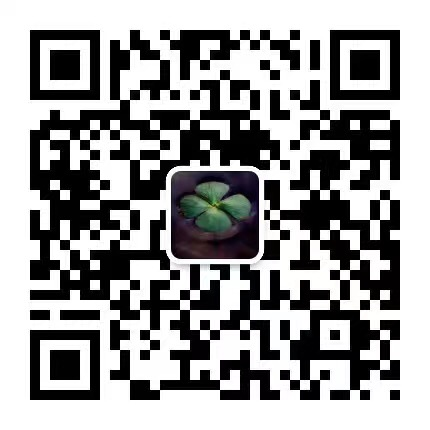
\includegraphics[width=4cm]{example/gzh.jpg}
\bicaption{中文题图}
{English caption}
\label{fig1}
\end{figure}

这里还有插入EPS图像和PDF图像的例子,如图\ref{fig2}和图\ref{fig3}。这里将EPS和PDF图片作为子图插入,每个子图有自己的小标题。子图标题使用subcaption宏包添加。

\begin{figure}[!htp]
\centering
\subcaptionbox{EPS 图像\label{fig2}}[3cm] %标题的长度,超过则会换行,如下一个小图。
{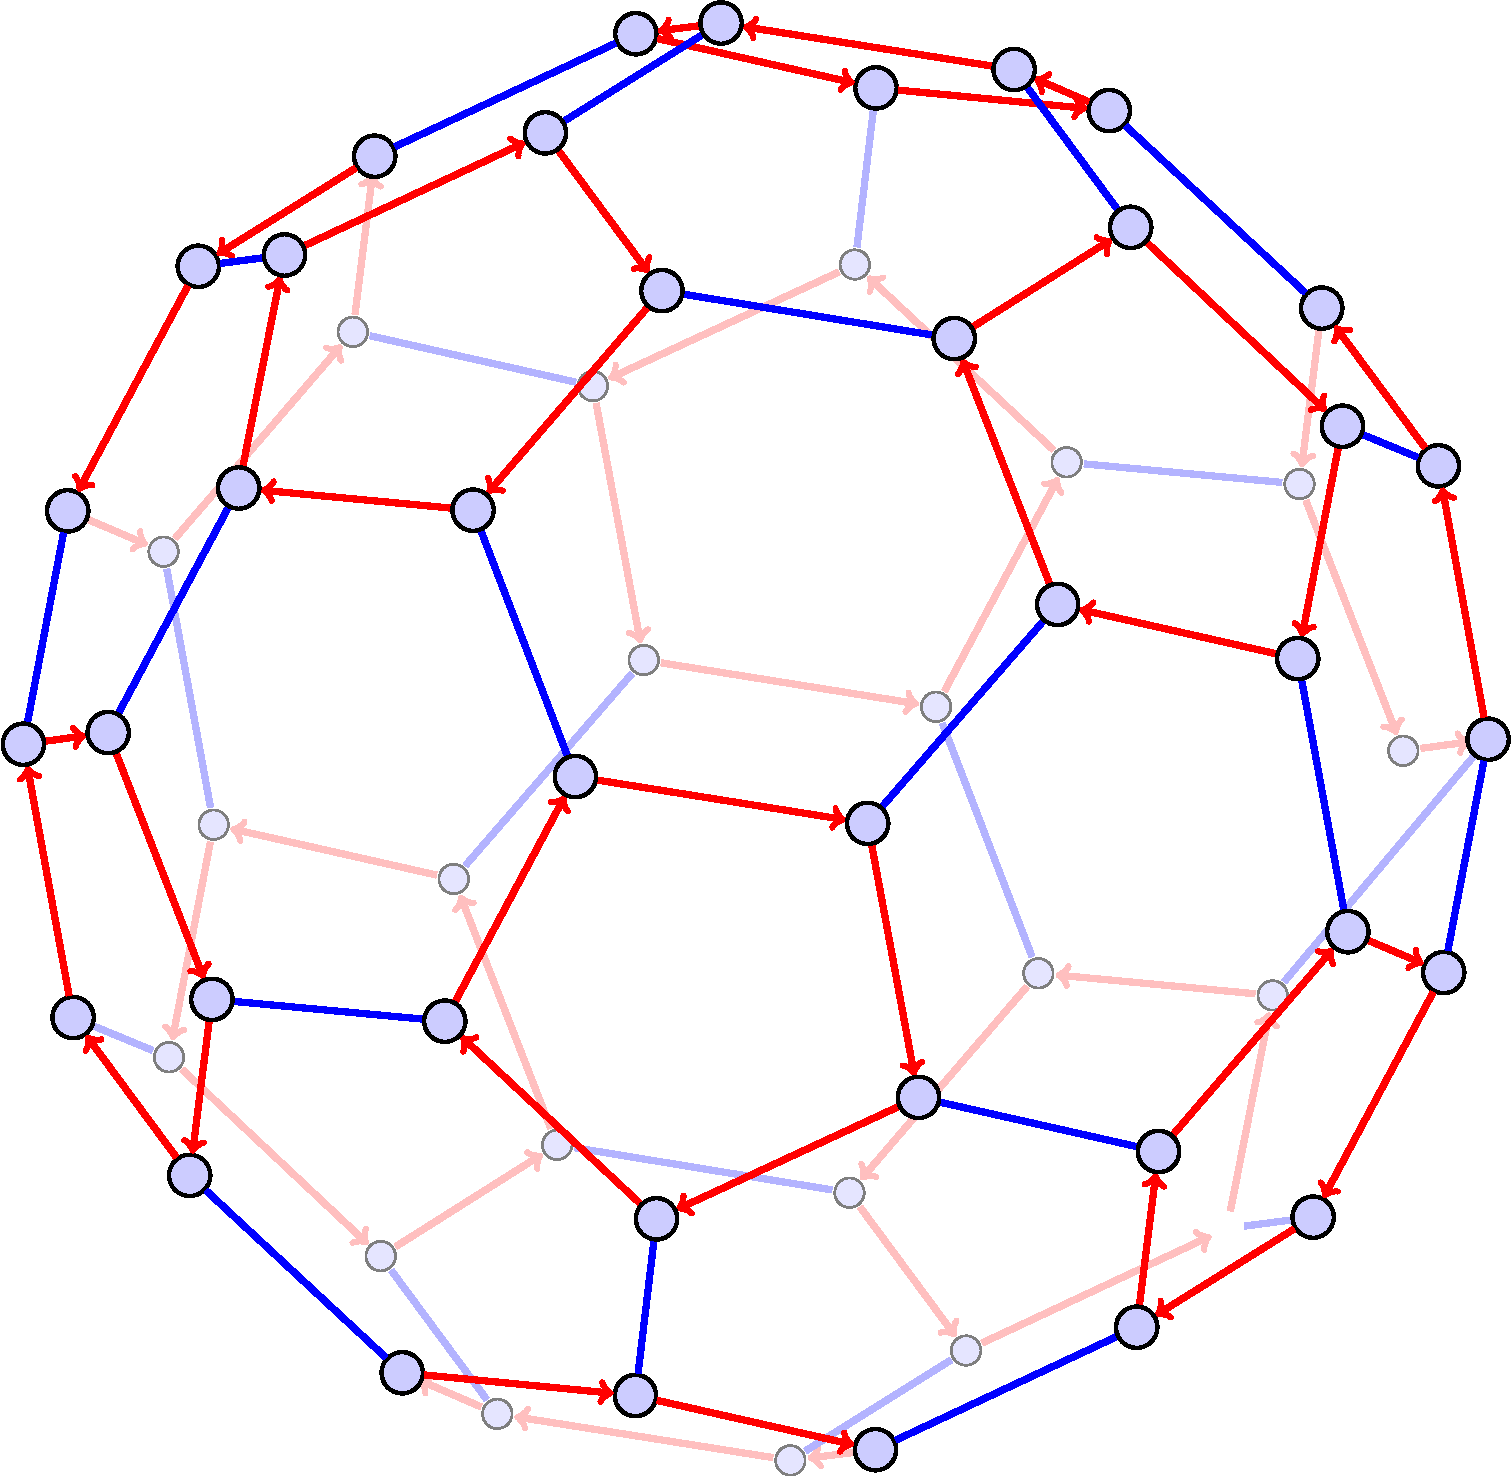
\includegraphics[height=2.5cm]{example/m2.pdf}}
\hspace{4em}
\subcaptionbox{PDF 图像,注意这个图略矮些。如果标题很长的话,它会自动换行\label{fig3}}
{	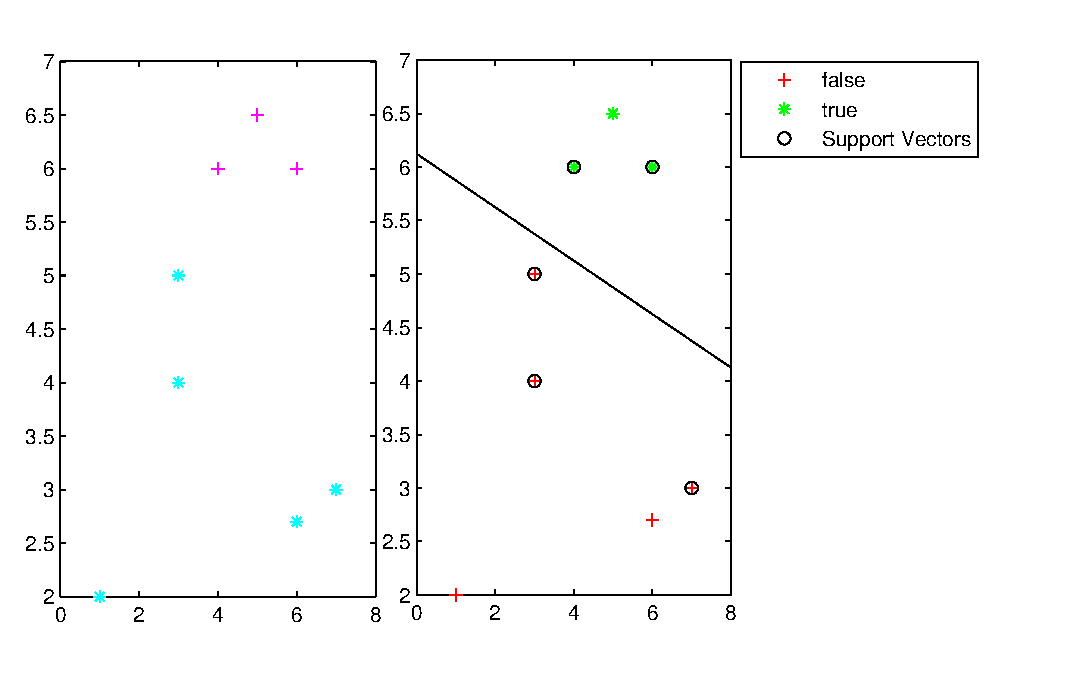
\includegraphics[scale=0.5]{example/figep.eps}}
\bicaption{插入eps和pdf的例子(使用 subcaptionbox 方式)}{An EPS and PDF demo with subcaptionbox}
\label{fig4}
\end{figure}




\section{插入代码}

这里给一个使用listings宏包插入源代码的例子:
\begin{lstlisting}[language={C}, caption={一段C源代码}]
#include <stdio.h>
#include <unistd.h>
#include <sys/types.h>
#include <sys/wait.h>

int main() {
pid_t pid;

switch ((pid = fork())) {
case -1:
printf("fork failed\n");
break;
case 0:
/* child calls exec */
execl("/bin/ls", "ls", "-l", (char*)0);
printf("execl failed\n");
break;
default:
/* parent uses wait to suspend execution until child finishes */
wait((int*)0);
printf("is completed\n");
break;
}

return 0;
}
\end{lstlisting}


\section{参考文献管理}
\label{sec2.5}
\LaTeX 具有将参考文献内容和表现形式分开管理的能力,涉及三个要素:参考文献数据库、参考文献引用格式、在正文中引用参考文献。
这样的流程需要多次编译:
\begin{enumerate}[noitemsep,topsep=0pt,parsep=0pt,partopsep=0pt]
\item 用户将论文中需要引用的参考文献条目,录入纯文本数据库文件(bib文件)。
\item 调用xelatex对论文模板做第一次编译,扫描文中引用的参考文献,生成参考文献入口文件(aux)文件。
\item 调用bibtex,以参考文献格式和入口文件为输入,生成格式化以后的参考文献条目文件(bib)。
\item 再次调用xelatex编译模板,将格式化以后的参考文献条目插入正文。
\end{enumerate}

参考文献数据库(thesis.bib)的条目,可以从Google Scholar搜索引擎\footnote{\url{https://scholar.google.com}}、CiteSeerX搜索引擎\footnote{\url{http://citeseerx.ist.psu.edu}}中查找,文献管理软件Papers\footnote{\url{http://papersapp.com}}、Mendeley\footnote{\url{http://www.mendeley.com}}、JabRef\footnote{\url{http://jabref.sourceforge.net}}也能够输出条目信息。

下面是在Google Scholar上搜索到的一条文献信息,格式是纯文本:

\begin{lstlisting}[caption={从Google Scholar找到的参考文献条目}, label=googlescholar, escapeinside="", numbers=none]
@phdthesis{"白2008信用风险传染模型和信用衍生品的定价",
title={"信用风险传染模型和信用衍生品的定价"},
author={"白云芬"},
year={2008},
school={"上海交通大学"}
} 
\end{lstlisting}

推荐修改后在bib文件中的内容为:

\begin{lstlisting}[caption={修改后的参考文献条目}, label=itemok, escapeinside="", numbers=none]
@phdthesis{bai2008,
title={"信用风险传染模型和信用衍生品的定价"},
author={"白云芬"},
date={2008},
address={"上海"},
school={"上海交通大学"}
} 
\end{lstlisting}

参考文献的引用:
\begin{itemize}
\item 参考文献在正文中被引用,使用命令\verb+\cite{key}+,如\cite{M91}。
\item 参考文献未引用但仍希望列在书末的参考文献中,使用命令\verb+\nocite{key}+,如\verb+\nocite{WI64,G03,D01,JS03}+.
\end{itemize}
\nocite{WI64,G03,D01,JS03}
%# -*- coding: utf-8-unix -*-


\chapter{两体问题}

无外力的两质点系统在相互作用下的运动求解问题称为{\heiti 两体问题}。

两体中心力是自然界最普遍、最典型的力场之一。中心力问题研究肇始于行星运动的理论解释,对原子核式模型的确立起了关键性的作用。

\section{两体问题约化与中心力场}

\subsection{Lagrange函数及其分离变量}

在两系统统不受外力作用时,设两个质点之间的相互作用势表示为$V = V(\mbf{r}_1 - \mbf{r}_2)$,则系统的Lagrange函数为
\begin{equation}
	L = \frac12 m_1 \dot{\mbf{r}}_1^2 + \frac12 m_2 \dot{\mbf{r}}_2^2 - V(\mbf{r}_1 - \mbf{r}_2)
\end{equation}
可见此Lagrange函数无循环坐标,两粒子的运动相互耦合。
\begin{figure}[htb]
\centering
\begin{asy}
	size(200);
	//两体问题
	pair O,m1,m2,C;
	O = (0,0);
	m1 = (1,0.8);
	m2 = (-0.2,0.6);
	C = interp(m2,m1,0.35);
	label("$O$",O,S);
	draw(Label("$\boldsymbol{r}_1$",MidPoint,Relative(E),black),O--m1,blue,Arrow);
	label("$m_1$",m1,SE);
	draw(Label("$\boldsymbol{r}_2$",MidPoint,Relative(W),black),O--m2,blue,Arrow);
	label("$m_2$",m2,W);
	draw(Label("$\boldsymbol{R}$",MidPoint,Relative(W),black),O--C,red,Arrow);
	label("$C$",C,N);
	draw(Label("$\boldsymbol{r}$",MidPoint,Relative(W),black),m2--m1,red,Arrow);
	dot(C);
	//draw(O--m1+(0.2,0),invisible);
\end{asy}
\caption{两体问题}
\label{两体问题}
\end{figure}

考虑取质心坐标
\begin{equation}
	\mbf{R} = \frac{m_1\mbf{r}_1+m_2\mbf{r}_2}{m_1+m_2}
\end{equation}
和两个质点之间的相对位矢
\begin{equation}
	\mbf{r} = \mbf{r}_1 - \mbf{r}_2
\end{equation}
为广义坐标。记$M = m_1+m_2$为系统的{\heiti 总质量},$\mu = \dfrac{m_1m_2}{m_1+m_2}$为两体{\heiti 约化质量},则有
\begin{equation}
	\begin{cases}
		\displaystyle \mbf{r}_1 = \mbf{R} + \frac{m_2}{M}\mbf{r} = \mbf{R} + \frac{\mu}{m_1} \mbf{r} \\[1.5ex]
		\displaystyle \mbf{r}_2 = \mbf{R} - \frac{m_1}{M}\mbf{r} = \mbf{R} - \frac{\mu}{m_2} \mbf{r}
	\end{cases}
	\label{两体问题广义坐标变换}
\end{equation}
由此,系统的Lagrange方程可以表示为
\begin{align}
	L & = \frac12 m_1 \left(\dot{\mbf{R}}+\frac{\mu}{m_1}\dot{\mbf{r}}\right)^2 + \frac12 m_2 \left(\dot{\mbf{R}}-\frac{\mu}{m_2}\dot{\mbf{r}}\right)^2 - V(\mbf{r}) \nonumber \\
	& = \frac12 M\dot{\mbf{R}}^2 + \frac12 \mu \dot{\mbf{r}}^2 - V(\mbf{r})
\end{align}
由此可以将两体问题等效为两个单体问题——解耦:
\begin{enumerate}
	\item 整体运动:质量为$M$的质点的运动。Lagrange函数不显含$\mbf{R}$,故有$\dot{P} = \mbf{0}$,即$M$做惯性运动。
	\item 相对运动:质量为$\mu$的质点的运动。
	\begin{equation*}
		\mu \ddot{\mbf{r}} = -\frac{\pl V}{\pl \mbf{r}}
	\end{equation*}
	即质点$\mu$在势场$V$中的运动。
\end{enumerate}
系统的动能$T=T_C+T'$,其中$\displaystyle T_C = \frac12 M\dot{\mbf{R}}^2$为整体动能,$\displaystyle T' = \frac12 \mu\dot{\mbf{r}}^2$为两体内动能。系统的角动量$\mbf{L} = \mbf{L}_C+\mbf{L}'$,其中$\mbf{L}_C = \mbf{R} \times M\dot{\mbf{R}}$为轨道角动量,
\begin{equation*}
	\mbf{L}' = \mbf{r}'_1 \times m_1 \dot{\mbf{r}}'_1 + \mbf{r}'_2 \times m_2 \dot{\mbf{r}}'_2 = \mu \mbf{r} \times \dot{\mbf{r}}
\end{equation*}
为内秉角动量。

由于两系统统的整体运动即为惯性运动,因此后面的讨论集中于相对运动的求解。

\subsection{两体中心力场}

如果两体相互作用势能只与两个粒子的相对距离$r$有关,而和它们的相对方向无关,即$V(\mbf{r}) = V(r)$,这种势场称为{\heiti 中心势场}。在中心势场中,可有两个质点之间的相互作用力为\footnote{此处由于\begin{equation*} r = \sqrt{x^2+y^2+z^2} \end{equation*}可有\begin{equation*} \frac{\pl r}{\pl \mbf{r}} = \bnb r = \frac{\pl r}{\pl x}{\mbf{e}_1}+\frac{\pl r}{\pl y}{\mbf{e}_2}+\frac{\pl r}{\pl z}{\mbf{e}_3} = \frac{x}{r}\mbf{e}_1 + \frac{y}{r}\mbf{e}_2 + \frac{z}{r}\mbf{e}_3 = \frac{\mbf{r}}{r} \end{equation*}}
\begin{equation}
	\mbf{f}_{12} = -\frac{\pl V}{\pl \mbf{r}} = -V'(r) \frac{\pl r}{\pl \mbf{r}} = -V'(r) \frac{\mbf{r}}{r} = -\mbf{f}_{21}
\end{equation}
由此,内力做功为
\begin{equation}
	\mbf{f}_{12} \cdot \mathrm{d} \mbf{r}_1 + \mbf{f}_{21} \cdot \mathrm{d} \mbf{r}_2 = -V'(r) \mathrm{d} r = -\mathrm{d} V(r)
\end{equation}
故$\mu$的运动能量守恒。再考虑内力矩
\begin{equation}
	\dif{\mbf{L}'}{t} = \mbf{M}' = \mbf{r} \times \left(-V'(r) \frac{\mbf{r}}{r}\right) = \mbf{0}
\end{equation}
故$\mu$的运动内秉角动量守恒,而且有$\mbf{r} \perp \mbf{L}'$,即$\mu$在垂直于内秉角动量的固定平面内运动。因此相对运动可用平面极坐标系来描述,即取$r,\theta$为广义坐标,则此时的Lagrange函数\footnote{在本章中,Lagrange函数和角动量得符号都是$L$,但角动量是矢量,所以并不会造成混淆。}为
\begin{equation}
	L' = \frac12 \mu \left(\dot{r}^2 + r^2 \dot{\theta}^2\right) - V(r)
\end{equation}

\section{等效势、运动解与轨道方程}

\subsection{运动方程}

根据相对运动的Lagrange函数
\begin{equation*}
	L' = \frac12 \mu \left(\dot{r}^2 + r^2 \dot{\theta}^2\right) - V(r)
\end{equation*}
可得运动方程为
\begin{equation}
	\begin{cases}
		\displaystyle \mu \left(\ddot{r}-r\dot{\theta}^2\right) = -V'(r) = f(r) \\
		\displaystyle \mu \left(r\ddot{\theta} + 2\dot{r} \dot{\theta}\right) = 0
	\end{cases}
	\label{两体运动方程}
\end{equation}

\subsection{守恒定律}

$\theta$为循环坐标,故有$p_\theta$守恒,即
\begin{equation}
	p_\theta = \mu r^2 \dot{\theta} = l\,\text{(常数)}
	\label{内秉角动量守恒}
\end{equation}
此即为两体内秉角动量守恒。

Lagrange函数$L'$不显含时间,故
\begin{equation}
	H = \frac12 \mu \left(\dot{r}^2+r^2\dot{\theta}^2\right) + V(r) = E\,\text{(常数)}
	\label{两体内能守恒}
\end{equation}
即两体机械能守恒。

\subsection{运动解}

由式\eqref{内秉角动量守恒}可得
\begin{equation*}
	\dot{\theta} = \frac{l}{\mu r^2}
\end{equation*}
代入式\eqref{两体内能守恒}可得
\begin{equation}
	\frac12 \mu \dot{r}^2 + \frac{l^2}{2\mu r^2} + V(r) = E
	\label{相对径向运动}
\end{equation}
令
\begin{equation}
	U(r) = \frac{l^2}{2\mu r^2} + V(r)
\end{equation}
称为{\heiti 等效势},则式\eqref{相对径向运动}化为
\begin{equation}
	\frac12 \mu \dot{r}^2 + U(r) = E
	\label{两体运动等效为一维运动}
\end{equation}
由此,径向运动等效为质点$\mu$在等效势场$U(r)$中的一维运动。等效势中的惯性离心势来自可遗角坐目标共轭动量效应。

在
\begin{equation}
	\frac{\mathrm{d} r}{\mathrm{d} t} = \pm \sqrt{\frac{2}{\mu}\big[E-U(r)\big]}
	\label{r对t的方程}
\end{equation}
两边积分可得
\begin{equation}
	t-t_0 = \pm \sqrt{\frac{\mu}{2}} \int_{r_0}^r \frac{\mathrm{d} r}{\sqrt{E-U(r)}}
	\label{t与r的关系}
\end{equation}
即有$r = r(t)$。再在
\begin{equation}
	\frac{\mathrm{d} \theta}{\mathrm{d} t} = \frac{l}{\mu r^2}
	\label{theta对t的方程}
\end{equation}
两边积分可得
\begin{equation}
	\theta - \theta_0 = \frac{l}{\mu} \int_{t_0}^t \frac{\mathrm{d} t}{\big[r(t)\big]^2}
	\label{chp4:theta与t的关系}
\end{equation}
即有$\theta = \theta(t)$。由此即得到了全部相对运动的解。

\subsection{轨道方程}

将式\eqref{r对t的方程}与式\eqref{theta对t的方程}相除,可得
\begin{equation}
	\frac{\mathrm{d} r}{\mathrm{d} \theta} = \pm \frac{\mu r^2}{l} \sqrt{\frac{2}{\mu}\big[E-U(r)\big]}
	\label{两体轨道方程(变量为r)}
\end{equation}
做变量代换$u=\dfrac{1}{r}$,可得两体问题轨道微分方程
\begin{equation}
	\frac{\mathrm{d} u}{\mathrm{d} \theta} = \mp \frac{1}{l} \sqrt{2\mu\left[E - U\left(\frac{1}{u}\right)\right]}
	\label{两体轨道方程}
\end{equation}
对于势场$V(r) = \dfrac{\alpha}{r} + \dfrac{\beta}{r^2}$和$V(r) = \alpha r^2$,式\eqref{两体轨道方程}有解析解。如果$r$的变化区间有两个边界$r_{\mathrm{min}}$和$r_{\mathrm{max}}$,则轨道位于两个圆$r = r_{\mathrm{min}}$和$r = r_{\mathrm{max}}$所限制的环形区域内,但有限运动的轨道并不一定是闭合的。在$r$从$r_{\mathrm{max}}$变化到$r_{\mathrm{min}}$再变回$r_{\mathrm{max}}$的这段时间内,矢径转过了一个角度$\Delta \theta$,根据式\eqref{两体轨道方程}有
\begin{equation}
	\Delta \theta = \mp 2\int_{\frac{1}{r_{\mathrm{max}}}}^{\frac{1}{r_{\mathrm{min}}}} \frac{l\mathrm{d} u}{\sqrt{2\mu\left[E-U\left(\dfrac{1}{u}\right)\right]}}
	\label{chapter4:近日点进动角}
\end{equation}
如果$\Delta \theta$与$2\pi$的比值是有理数,轨道是闭合的。一般来说,在任意形式的$V(r)$情况下,轨道闭合的情况是罕见的。在任意形式的$V(r)$情况下,$\Delta \theta$与$2\pi$的比值并不是有理数,因此在一般情况下,有限运动的轨道并不是闭合的。在无限长的时间进程中,轨道无数次经过$r_{\max}$和$r_{\min}$的位置而填满由两个圆所限制的整个圆环,如图\ref{非闭合轨道}所示。只有$V(r) = \dfrac{\alpha}{r}$和$V(r) = \alpha r^2$两种形式的势场中,任意有限运动的轨道都是闭合的。

\begin{figure}[htb]
\centering
\begin{asy}
	size(300);
	//进动的非闭合轨道
	real p,e,omega,rmax,rmin;
	pair O;
	path g;
	O = (0,0);
	p = 1;
	e = 0.7;
	omega = 1-0.06;
	rmax = p/(1-e);
	rmin = p/(1+e);
	pair rotell(real theta){
		real r = p/(1+e*cos(omega*theta));
		return (-r*cos(theta),r*sin(theta));
	}
	g = graph(rotell,16*pi/omega,-1.25*pi,10000);
	draw(g);
	for(real rp=1;rp>0;rp=rp-0.06){
		add(arrow(g,invisible,FillDraw(black),Relative(rp)));
	}
	draw(scale(rmax)*unitcircle,dashed);
	draw(scale(rmin)*unitcircle,dashed);
	draw(rotell(15*pi/omega)--1.06*rotell(15*pi/omega));
	draw(rotell(13*pi/omega)--1.06*rotell(13*pi/omega));
	draw(Label("$\Delta \theta$",MidPoint,Relative(E)),arc(O,length(1.03*rotell(15*pi/omega)),degrees(rotell(15*pi/omega)),degrees(rotell(13*pi/omega))),Arrows);
	draw(Label("$r_{\min}$",MidPoint,Relative(E)),O--rmin*dir(-20),Arrow);
	draw(Label("$r_{\max}$",Relative(0.7),Relative(W)),O--rmax*dir(110),Arrow);
	draw(O--(rmax+0.01)*dir(90),invisible);
\end{asy}
\caption{非闭合轨道}
\label{非闭合轨道}
\end{figure}

也可通过系统的运动方程\eqref{两体运动方程}得到轨道满足的微分方程。考虑
\begin{equation*}
	\dot{r} = \dot{\theta} \frac{\mathrm{d} r}{\mathrm{d} \theta} = \frac{l}{\mu r^2} \frac{\mathrm{d} r}{\mathrm{d} \theta} = -\frac{l}{\mu} \frac{\mathrm{d} u}{\mathrm{d} \theta}
\end{equation*}
所以
\begin{equation*}
	\ddot{r} = \dot{\theta} \frac{\mathrm{d} \dot{r}}{\mathrm{d} \theta} = \frac{l}{\mu r^2} \frac{\mathrm{d}}{\mathrm{d} \theta} \left(-\frac{l}{\mu} \frac{\mathrm{d} u}{\mathrm{d} \theta}\right) = -\frac{l^2u^2}{\mu^2} \frac{\mathrm{d}^2 u}{\mathrm{d} \theta^2}
\end{equation*}
由此可得
\begin{equation*}
	-\frac{l^2u^2}{\mu} \frac{\mathrm{d}^2 u}{\mathrm{d} \theta^2} - \mu r\left(\frac{l}{\mu r^2}\right)^2 = f(r)
\end{equation*}
整理可得二阶常微分方程
\begin{equation}
	\frac{\mathrm{d}^2 u}{\mathrm{d} \theta^2} + u = -\frac{\mu}{l^2 u^2} f\left(\frac{1}{u}\right)
	\label{Binet方程}
\end{equation}
称为{\heiti Binet方程}。

\subsection{圆轨道的存在性与稳定性}

圆轨道存在,即径向运动处于静止状态,即可以表示为
\begin{equation*}
	\frac{\mathrm{d} U}{\mathrm{d} r} \bigg|_{r=r_m} = 0
\end{equation*}
稳定要求在圆轨道上等效势能取极小值,即
\begin{equation*}
	\frac{\mathrm{d}^2 U}{\mathrm{d} r^2} \bigg|_{r=r_m} > 0
\end{equation*}

\begin{example}
利用等效势定性分析质点在势场
\begin{equation*}
	V(r) = -\frac{\alpha}{r^n},\quad \alpha,n > 0
\end{equation*}
中的运动。
\end{example}
\begin{solution}
势场对应的力
\begin{equation*}
	f(r) = -V'(r) = -\frac{\alpha n}{r^{n+1}}<0
\end{equation*}
即势场为吸引势。则等效势为
\begin{equation*}
	U(r) = \frac{l^2}{2\mu r^2} - \frac{\alpha}{r^n}
\end{equation*}
径向运动方程
\begin{equation*}
	\frac12 \mu \dot{r}^2 + U(r) = E
\end{equation*}
需要满足$\dfrac12 \mu \dot{r}^2 \geqslant 0$,即
\begin{equation*}
	U(r) \leqslant E
\end{equation*}
上面的不等式即决定了质点径向运动的范围。计算
\begin{equation*}
	U'(r) = -\frac{l^2}{\mu r^3} + \frac{\alpha n}{r^{n+1}} = 0
\end{equation*}
可得$U(r)$的极值点为
\begin{equation*}
	r_m = \left(\frac{l^2}{n\alpha \mu}\right)^{\frac{1}{2-n}}
\end{equation*}
极值点存在要求$n \neq 2$,因此势场分为$0<n<2$、$n>2$和$n=2$三种情形。
\begin{enumerate}
	\item $0<n<2$。当$E=E_0=U_{\mathrm{min}}$时,质点沿圆轨道运动,由于是极小值轨道是稳定的。
	
	当$E=E_1<0$时,运动被限制在$r_{\mathrm{min}} \leqslant r \leqslant r_{\mathrm{max}}$的范围内,这种状态称为束缚态。按前面的讨论,束缚态的轨道不一定是闭合的。
	
	当$E=E_2=0$时,粒子的运动范围为$r \geqslant r_{\mathrm{min}}$,当$r \to +\infty$时,粒子的速度趋于$0$,轨迹趋于直线。
	
	当$E=E_3>0$时,粒子的运动范围同样为$r \geqslant r_{\mathrm{min}}$,但当$r \to +\infty$时,粒子的动能趋于$E$,轨迹趋于直线。这种状态称为散射态。

	\item $n>2$。当$E=E_0=U_{\mathrm{max}}$时,质点沿圆轨道运动,由于是极大值轨道是不稳定的。
	
	当$0<E=E_1<U_{\mathrm{max}}$时,粒子只能出现在$r = r_{\mathrm{min}}$的圆内或$r = r_{\mathrm{max}}$的圆外,在中间的环形区域内粒子是禁戒的。若初始时刻粒子在$r = r_{\mathrm{min}}$的圆内,则$\dot{r} < 0$时,粒子被吸引至力心;当$\dot{r}>0$时,粒子先飞到$r = r_{\mathrm{min}}$的圆周上,然后折回到力心。而如果初始时刻粒子在$r = r_{\mathrm{max}}$的圆外,则$\dot{r} < 0$时,粒子先飞到$r = r_{\mathrm{max}}$的圆周上,然后飞向无穷远处;当$\dot{r}>0$时,粒子直接飞翔无穷远处最终成为自由粒子。
	
	当$E=E_2=0$时或者$E=E_4<0$时,粒子的运动范围为$r = r_{\mathrm{max}}$的圆内,并最终被力心俘获。
	
	当$E=E_3>U_{\mathrm{max}}$时,粒子可在全空间运动。当$\dot{r}>0$时,粒子飞向无穷远最终变为自由粒子;当$\dot{r}<0$时,粒子飞向中心,最后被力心俘获。

\begin{figure}[htb]
\centering
\begin{minipage}[t]{0.45\textwidth}
\centering
\begin{asy}
	size(190);
	//0<n<2的情形
	real alpha,beta,n;
	picture tmp;
	real fr(real r){
		return beta/(r**2)-alpha/(r**n);
	}
	real f1r(real r){
		return beta/(r**2);
	}
	real f2r(real r){
		return -alpha/(r**n);
	}
	alpha = 0.8*4;
	beta = 1*4;
	n = 1;
	draw(tmp,xscale(0.4)*graph(fr,0.3,18,operator..),linewidth(1bp));
	draw(tmp,xscale(0.4)*graph(f1r,0.3,18,operator..),dashed);
	draw(tmp,xscale(0.4)*graph(f2r,0.3,18,operator..),dashed);
	xequals(tmp,0,black);
	yequals(tmp,0,black);
	real rm,r1,r2;
	rm = (2*beta/alpha/n)**(1/(2-n));
	draw(tmp,xscale(0.4)*((0,fr(rm))--(rm,fr(rm))--(rm,0)),red);
	r1 = (beta/alpha)**(1/(2-n))+0.225;
	r2 = 8;
	draw(tmp,xscale(0.4)*((0,fr(r2))--(r2,fr(r2))--(r2,0)),green);
	draw(tmp,xscale(0.4)*((r1,0)--(r1,fr(r1))),green);
	draw(tmp,xscale(0.4)*((0,fr(1))--(18,fr(1))),blue);
	draw(tmp,xscale(0.4)*((1,fr(1))--(1,0)),blue);
	path clp;
	clp = box((-0.1,-fr(0.7)),(7.2,fr(0.7)));
	clip(tmp,clp);
	add(tmp);
	label("$\dfrac{l^2}{2\mu r^2}$",xscale(0.4)*(2,f1r(2)),NE);
	label("$V$",xscale(0.4)*(2,f2r(2)),SE);
	label("$E_0$",(0,fr(rm)),SW,red);
	label("$E_1$",(0,fr(r2)),W,green);
	label("$E_2$",(0,0),NW);
	label("$E_3$",(0,fr(1)),W,blue);
	label("$r$",(7.2,0),E);
	label("$U$",(0,fr(0.7)),W);
\end{asy}
\caption{$0<n<2$的情形}
\label{0<n<2的情形}
\end{minipage}
\hspace{0.7cm}
\begin{minipage}[t]{0.45\textwidth}
\centering
\begin{asy}
	size(190);
	//n>2的情形
	real alpha,beta,n;
	picture tmp;
	real fr(real r){
		return beta/(r**2)-alpha/(r**n);
	}
	real f1r(real r){
		return beta/(r**2);
	}
	real f2r(real r){
		return -alpha/(r**n);
	}
	alpha = 0.8*4;
	beta = 1*4;
	n = 3;
	draw(tmp,xscale(0.8)*graph(fr,0.3,18,operator..),linewidth(1bp));
	draw(tmp,xscale(0.8)*graph(f1r,0.3,18,operator..),dashed);
	draw(tmp,xscale(0.8)*graph(f2r,0.3,18,operator..),dashed);
	xequals(tmp,0,black);
	yequals(tmp,0,black);
	real rm,r1,r2,r3,E3;
	rm = (2*beta/alpha/n)**(1/(2-n));
	draw(tmp,xscale(0.8)*((0,fr(rm))--(rm,fr(rm))--(rm,0)),red);
	r1 = (beta/alpha)**(1/(2-n))+0.069;
	r2 = 2.5;
	draw(tmp,xscale(0.8)*((0,fr(r2))--(18,fr(r2))),green);
	draw(tmp,xscale(0.8)*((r2,fr(r2))--(r2,0)),green);
	draw(tmp,xscale(0.8)*((r1,0)--(r1,fr(r1))),green);
	r3 = 0.7;
	draw(tmp,xscale(0.8)*((0,fr(r3))--(r3,fr(r3))--(r3,0)),orange);
	E3 = 1.8;
	draw(tmp,xscale(0.8)*((0,E3)--(18,E3)),blue);
	path clp;
	clp = box((-0.1,-fr(0.6)),(7.2,fr(0.6)));
	clip(tmp,clp);
	add(tmp);
	label("$\dfrac{l^2}{2\mu r^2}$",xscale(0.8)*(1.3,f1r(1.3)),NE);
	label("$V$",xscale(0.8)*(1.3,f2r(1.3)),SE);
	label("$E_0$",(0,fr(rm)),W,red);
	label("$E_1$",(0,fr(r2)),W,green);
	label("$E_2$",(0,0),W);
	label("$E_3$",(0,E3),W,blue);
	label("$E_4$",(0,fr(r3)),W,orange);
	label("$r$",(7.2,0),E);
	label("$U$",(0,abs(fr(0.6))),W);
	//draw((0,0)--(7.9,0),invisible);
\end{asy}
\caption{$n>2$的情形}
\label{n>2的情形}
\end{minipage}

\begin{minipage}[t]{0.45\textwidth}
\centering
\begin{asy}
	size(190);
	//n=2的情形1
	real alpha,beta,n;
	picture tmp;
	real fr(real r){
		return beta/(r**2)-alpha/(r**n);
	}
	real f1r(real r){
		return beta/(r**2);
	}
	real f2r(real r){
		return -alpha/(r**n);
	}
	alpha = 1.6*1.7;
	beta = 1*1.7;
	n = 2;
	draw(tmp,graph(fr,0.3,18,operator..),linewidth(1bp));
	draw(tmp,graph(f1r,0.3,18,operator..),dashed);
	draw(tmp,graph(f2r,0.3,18,operator..),dashed);
	xequals(tmp,0,black);
	yequals(tmp,0,black);
	real E3,r1;
	r1 = 1.5;
	draw(tmp,(r1,0)--(r1,fr(r1))--(0,fr(r1)),green);
	E3 = 1.1;
	draw(tmp,(0,E3)--(18,E3),blue);
	path clp;
	clp = box((-0.1,-fr(0.6)),(6,fr(0.6)));
	clip(tmp,clp);
	add(tmp);
	label("$\dfrac{l^2}{2\mu r^2}$",(1,f1r(1)),NE);
	label("$V$",(1.3,f2r(1.3)),SE);
	label("$E_1$",(0,fr(r1)),W,green);
	label("$E_2$",(0,0),W);
	label("$E_3$",(0,E3),W,blue);
	label("$r$",(6,0),E);
	label("$U$",(0,abs(fr(0.6))),W);
	//draw((0,0)--(6.9,0),invisible);
\end{asy}
\caption{$n=2$的情形($\alpha>\dfrac{l^2}{2\mu}$)}
\label{n=2的情形1}
\end{minipage}
\hspace{0.7cm}
\begin{minipage}[t]{0.45\textwidth}
\centering
\begin{asy}
	size(190);
	//n=2的情形2
	real alpha,beta,n;
	picture tmp;
	real fr(real r){
		return beta/(r**2)-alpha/(r**n);
	}
	real f1r(real r){
		return beta/(r**2);
	}
	real f2r(real r){
		return -alpha/(r**n);
	}
	alpha = 1*1.7;
	beta = 1.6*1.7;
	n = 2;
	draw(tmp,graph(fr,0.3,18,operator..),linewidth(1bp));
	draw(tmp,graph(f1r,0.3,18,operator..),dashed);
	draw(tmp,graph(f2r,0.3,18,operator..),dashed);
	xequals(tmp,0,black);
	yequals(tmp,0,black);
	real r1;
	r1 = 1;
	draw(tmp,(r1,0)--(r1,fr(r1))--(0,fr(r1)),green);
	path clp;
	clp = box((-0.1,-fr(0.6)),(6,fr(0.6)));
	clip(tmp,clp);
	add(tmp);
	label("$\dfrac{l^2}{2\mu r^2}$",(1.2,f1r(1.2)),NE);
	label("$V$",(1.3,f2r(1.3)),SE);
	label("$E_1$",(0,fr(r1)),W,green);
	label("$E_2$",(0,0),W);
	label("$r$",(6,0),E);
	label("$U$",(0,abs(fr(0.6))),W);
	//draw((0,0)--(6.9,0),invisible);
\end{asy}
\caption{$n=2$的情形($\alpha<\dfrac{l^2}{2\mu}$)}
\label{n=2的情形2}
\end{minipage}
\end{figure}
	\item $n=2$而且$\alpha>\dfrac{l^2}{2\mu}$。当$E=E_1<0$时,粒子只能出现在$r = r_{\mathrm{max}}$的圆内,并最终被力心俘获。
	
	当$E=E_2=0$时,粒子可在全空间运动,最终粒子将飞向无穷远处且趋于静止。
	
	当$E=E_3>0$时,粒子可在全空间运动,最终将飞向无穷远处最终称为自由粒子。
	\item $n=2$而且$\alpha<\dfrac{l^2}{2\mu}$。在这种情形下,只能$E>0$,此时粒子只能出现在$r = r_{\mathrm{max}}$的圆外,最终飞向无穷远而称为自由粒子。
\end{enumerate}
\end{solution}

\begin{example}
求势场
\begin{equation*}
	V(r) = \alpha r^n
\end{equation*}
存在稳定圆轨道的条件。
\end{example}
\begin{solution}
等效势为
\begin{equation*}
	U(r) = \frac{l^2}{2\mu r^2} + \alpha r^n
\end{equation*}
存在圆轨道要求
\begin{equation*}
	U'(r_m) = -\frac{l^2}{\mu r_m^3} + \alpha n r_m^{n-1} = 0
\end{equation*}
即有
\begin{equation*}
	\alpha n r_m^{n+2} = \frac{l^2}{\mu}
\end{equation*}
由此即要求$\alpha n>0$。此时
\begin{equation*}
	f(r) = -V'(r) = -\alpha n r^{n-1} < 0
\end{equation*}
即存在圆轨道要求势场为吸引力场。下面考虑稳定性,稳定性要求
\begin{equation*}
	U''(r_m) = \frac{1}{r_m^4} \left[(n-1)\alpha n r_m^{n+2} + \frac{3l^2}{\mu}\right] = (n+2) \frac{l^2}{\mu r_m^4} > 0
\end{equation*}
即圆轨道稳定要求$n>-2$。

综上,存在稳定圆轨道的条件为$\alpha>0,n>0$或者$\alpha<0,-2<n<0$。
\end{solution}

\section{距离反比势场与Kepler问题}

\begin{figure}[htb]
\centering
\begin{asy}
	size(300);
	//距离反比势场势能曲线图
	real alpha,beta,xmax,ymax;
	picture tmp;
	real fr(real r){
		return beta/(r**2)+alpha/r;
	}
	real f1r(real r){
		return beta/(r**2);
	}
	real f2r(real r){
		return alpha/r;
	}
	alpha = -2.5*4;
	beta = 2*4;
	ymax = abs(fr(0.53));
	draw(tmp,graph(fr,0.3,18,operator..),linewidth(1bp)+red,Label("引力等效势"));
	draw(tmp,graph(f2r,0.3,18,operator..),dashed+red,Label("引力势"));
	alpha = 2.5*4;
	draw(tmp,graph(fr,0.3,18,operator..),linewidth(1bp)+blue,Label("斥力等效势"));
	draw(tmp,graph(f2r,0.3,18,operator..),dashed+blue,Label("斥力势"));
	draw(tmp,graph(f1r,0.3,18,operator..),dashed,Label("离心势"));
	xequals(tmp,0,black);
	yequals(tmp,0,black);
	path clp;
	xmax = 15;
	clp = box((-0.1,-2/3*ymax),(xmax,ymax));
	clip(tmp,clp);
	add(tmp);
	label("$r$",(xmax,0),E);
	label("$U$",(0,ymax),W);
	fill(box((xmax+0.1,ymax-0.2),(xmax-7.4,ymax-5.8)),black);
	add(legend(),(xmax,ymax),SW,UnFill);
	//draw((0,0)--(xmax+0.9,0),invisible);
\end{asy}
\caption{距离反比势场势能曲线图}
\label{距离反比势场势能曲线图}
\end{figure}

距离反比势可以表示为
\begin{equation*}
	V(r) = \frac{\alpha}{r},\quad f(r) = -V'(r) = \frac{\alpha}{r^2}
\end{equation*}
此势场当$\alpha<0$时表现为引力场,当$\alpha>0$时表现为斥力场。其等效势为
\begin{equation}
	U(r) = \frac{l^2}{2\mu r^2} + \frac{\alpha}{r}
\end{equation}
对于引力的情形,在
\begin{equation}
	r_m = -\frac{l^2}{\mu \alpha}
\end{equation}
时,等效势有极小值
\begin{equation}
	U_{\mathrm{min}} = -\frac{\mu \alpha^2}{2l^2}
\end{equation}
对于斥力的情形,等效势没有极值,仍记
\begin{equation*}
	r_m = -\frac{l^2}{\mu \alpha}
\end{equation*}

当$\alpha<0$时(即引力情形)称为{\bf Kepler问题}。

\subsection{轨道方程}\label{chapter4:subsection-轨道方程}

对于Kepler问题,Binet方程\eqref{Binet方程}为
\begin{equation}
	\frac{\mathrm{d}^2 u}{\mathrm{d} \theta^2} + u = \frac{1}{r_m}
	\label{Kepler问题的轨道微分方程}
\end{equation}
方程\eqref{Kepler问题的轨道微分方程}的通解为
\begin{equation*}
	u = \frac{1}{r_m} + A\cos(\theta-\theta_0)
\end{equation*}
即
\begin{equation*}
	r = \frac{r_m}{1+Ar_m \cos (\theta-\theta_0)}
\end{equation*}
适当选取极轴的方向,可以使得$\theta_0=0$,此时轨道方程为
\begin{equation*}
	r = \frac{r_m}{1+Ar_m \cos \theta}
\end{equation*}
记
\begin{equation}
	p = |r_m| = \frac{l^2}{\mu |\alpha|},\quad e = Ap
	\label{chapter4:Kepler问题的轨道参数}
\end{equation}
其中$p$为{\heiti 轨道参数},$e$为{\heiti 离心率},由此可得Kepler问题的轨道方程为
\begin{equation}
	r = \frac{p}{1+e\cos \theta}
	\label{Kepler问题的轨道方程}
\end{equation}
% 当$\alpha>0$时(斥力),轨道方程为\footnote{在斥力的极坐标方程中,需要允许极径取负值。}
% \begin{equation}
	% r = \frac{p}{e\cos \theta-1}
% \end{equation}
% 首先考虑引力的情形,
根据轨道方程可得质点与力心的最短距离为
\begin{equation*}
	r_{\mathrm{min}} = \frac{p}{1+e}
\end{equation*}
此点一般称为{\heiti 近日点}或{\bf 近心点}。在近日点有$\dot{r}\big|_{r=r_{\mathrm{min}}} = 0$,因此$r_{\mathrm{min}}$满足
\begin{equation*}
	\frac{l^2}{2\mu r_{\mathrm{min}}^2} + \frac{\alpha}{r_{\mathrm{min}}} = E
\end{equation*}
由此可得离心率与系统总能量的关系
\begin{equation}
	e = \sqrt{1+\frac{2El^2}{\mu\alpha^2}} = \sqrt{1-\frac{E}{U_{\mathrm{min}}}}
\end{equation}
% 对于斥力的情形,根据轨道方程可得质点与原点的最短距离为\footnote{斥力情形下,轨道为双曲线的右支,此时矢径取负值}
% \begin{equation*}
	% r_{\mathrm{min}} = -\frac{p}{1+e}
% \end{equation*}
% 此时同样有
% \begin{equation*}
	% \frac{l^2}{2\mu r_{\mathrm{min}}^2} + \frac{\alpha}{r_{\mathrm{min}}} = E
% \end{equation*}
% 由此可得斥力情形下离心率与系统总能量的关系
% \begin{equation*}
	% e = \sqrt{1+\frac{2El^2}{\mu\alpha^2}}
% \end{equation*}
% 综上,无论对于引力还是斥力场,都有
% \begin{equation}
	% p = |r_m| = \frac{l^2}{\mu |\alpha|},\quad e = \sqrt{1+\frac{2El^2}{\mu\alpha^2}}
% \end{equation}

\begin{figure}[htb]
\centering
\begin{asy}
	size(250);
	//各种情形下轨道的形状
	pair O;
	real p,e[],ee,xmax,ymax;
	picture tmp;
	O = (0,0);
	real r(real theta){
		return p/(1+ee*cos(theta));
	}
	real nr(real theta){
		return p/(ee*cos(theta)-1);
	}
	pair xy(real theta){
		return (r(theta)*cos(theta),r(theta)*sin(theta));
	}
	pair nxy(real theta){
		return (nr(theta)*cos(theta),nr(theta)*sin(theta));
	}
	p = 1;
	e[1] = 0.4;
	ee = e[1];
	draw(tmp,graph(xy,0,2*pi),green+linewidth(1bp));
	e[2] = 1;
	ee = e[2];
	draw(tmp,graph(xy,-0.7*pi,0.7*pi),linewidth(1bp));
	e[3] = 2.5;
	ee = e[3];
	draw(tmp,graph(xy,-0.6*pi,0.6*pi),blue+linewidth(1bp));
	//draw(tmp,graph(nxy,-0.34*pi,0.34*pi),purple+linewidth(1bp));
	draw(tmp,scale(p)*unitcircle,red+linewidth(1bp));
	draw(tmp,(-100,0)--(100,0));
	draw(tmp,(0,-100)--(0,100));
	label(tmp,"$p$",(0,p/2),W);
	dot(tmp,O);
	xmax = p/(1-e[1])*1.1;
	ymax = xmax;
	path clp = box((-xmax,-ymax),(xmax,ymax));
	clip(tmp,clp);
	add(tmp);
	ee = e[1];
	label("$U_{\mathrm{min}}<E<0$",xy(-0.7*pi),SW,green);
	label("$E=0$",(-0.7*xmax,ymax),N);
	label("$E>0$",(-0.25*xmax,ymax),N,blue);
	//label("$\alpha<0$",(-0.25*xmax,-ymax),S,blue);
	//label("$E>0$",(0.7*xmax,ymax),N,purple);
	//label("$\alpha>0$",(0.7*xmax,-ymax),S,purple);
	label("$E=U_{\mathrm{min}}$",relpoint(scale(p)*unitcircle,0.06),E,red);
\end{asy}
\caption{各种情形下轨道的形状}
\label{各种情形下轨道的形状}
\end{figure}

%在斥力的情形下,$\alpha>0$,$E>0$,则有$e>1$,轨道为双曲线。

在引力的情形下,$\alpha<0$,按照系统能量的区别可以分为以下4种情况:
\begin{enumerate}
	\item 当$E>0$时,$e>1$,轨道为双曲线;
	\item 当$E=0$时,$e=1$,轨道为拋物线;
	\item 当$U_{\mathrm{min}}<E<0$时,$0<e<1$,轨道为椭圆;
	\item 当$E=U_{\mathrm{min}}$时,$e=0$,轨道为圆。
\end{enumerate}
各种情形下,轨道的形状如图\ref{各种情形下轨道的形状}所示。

当质点沿着轨道运动时,坐标对时间的依赖关系可以用式\eqref{t与r的关系}得到。它可以表示为下面所述的一种方便的参数形式。

首先研究椭圆轨道。对椭圆轨道,质点与力心的最大距离为
\begin{equation*}
	r_{\max} = \frac{p}{1-e}
\end{equation*}
此点一般称为{\bf 远日点}或{\bf 远心点}。因此可有椭圆的半长轴为
\begin{equation*}
	a = \frac12 \left(\frac{p}{1-e}+\frac{p}{1+e}\right) = \frac{\alpha}{2E} > 0
\end{equation*}
由此,根据式\eqref{t与r的关系}可得
\begin{align*}
	t-t_0 & = \sqrt{\frac{\mu}{2}} \int_{r_{\min}}^r \frac{\mathrm{d}r}{\sqrt{E-U(r)}} = \sqrt{\frac{\mu}{2|E|}} \int_{r_{\min}}^r \frac{r\mathrm{d}r}{\sqrt{-r^2-\dfrac{\alpha}{|E|}r-\dfrac{l^2}{2\mu|E|}}} \\
	& = \sqrt{\frac{\mu a}{|\alpha|}} \int_{r_{\min}}^r \frac{r\mathrm{d}r}{\sqrt{a^2e^2-(r-a)^2}}
\end{align*}
利用变换
\begin{equation*}
	r-a = -ae\cos \xi
\end{equation*}
可得
\begin{equation*}
	t-t_0 = \sqrt{\frac{\mu a^3}{|\alpha|}} \int_0^\xi (1-e\cos\xi) \mathrm{d}\xi = \sqrt{\frac{\mu a^3}{|\alpha|}} (\xi-e\sin \xi)
\end{equation*}
如果将近日点的时刻取为$t_0=0$,可得{\bf Kepler方程}
\begin{equation}
	t = \sqrt{\frac{\mu a^3}{|\alpha|}} (\xi-e\sin \xi)
	\label{Kepler方程}
\end{equation}
此时即可有关于到力心距离的参数方程
\begin{equation}
\begin{cases}
	r=a(1-e\cos \xi) \\
	t = \sqrt{\dfrac{\mu a^3}{|\alpha|}} (\xi-e\sin \xi)
\end{cases}
\end{equation}
再结合轨道方程\eqref{Kepler问题的轨道方程},可得轨道的参数方程
\begin{equation}
\begin{cases}
	x = r\cos \theta = a(\cos \xi-e) \\
	y = \sqrt{r^2-x^2} = a\sqrt{1-e^2}\sin \xi \\
	t = \sqrt{\dfrac{\mu a^3}{|\alpha|}} (\xi-e\sin \xi)
\end{cases}
\end{equation}
沿着椭圆轨道运动一整圈即对应着参数$\xi$从$0$到$2\pi$,其中参数$\xi$称为椭圆的{\bf 圆心角},其几何意义如图\ref{圆心角的几何意义}所示。

\begin{figure}[htb]
\centering
\begin{asy}
	size(250);
	//圆心角的几何意义
	real x,a,b,c,theta,r;
	a = 2;
	b = 1.2;
	x = 2.5;
	c = sqrt(a^2-b^2);
	draw((-x,0)--(x,0));
	draw((0,-x)--(0,x));
	draw(xscale(a)*yscale(b)*unitcircle,linewidth(0.8bp));
	draw(scale(a)*unitcircle);
	dot((c,0));
	theta = 60;
	draw((0,0)--a*dir(theta));
	pair P;
	P = intersectionpoint(xscale(a)*yscale(b)*unitcircle,a*dir(theta)--(a*dir(theta).x,0));
	draw((c,0)--P);
	draw(a*dir(theta)--(a*dir(theta).x,0));
	label("$p$",(P+(a*dir(theta).x,0))/2,W);
	r = 0.3;
	draw(Label("$\xi$",MidPoint,Relative(E)),arc((0,0),r,0,theta));
	r = 0.15;
	draw(Label("$\theta$",MidPoint,Relative(E)),arc((c,0),r,0,degrees(P-(c,0))));
	label("$a$",(a,0),SE);
	label("$b$",(0,b),SW);
	label("$a$",(0,a),NW);
	label("$ae$",(c,0),S);
	dot("$P$",P,NE);
\end{asy}
\caption{圆心角的几何意义}
\label{圆心角的几何意义}
\end{figure}

对于双曲线轨道,同样有双曲线的半轴长为
\begin{equation*}
	a = \frac{|\alpha|}{2E}
\end{equation*}
同样,根据式\eqref{t与r的关系}可得
\begin{align*}
	t-t_0 & = \sqrt{\frac{\mu}{2}} \int_{r_{\min}}^r \frac{\mathrm{d}r}{\sqrt{E-U(r)}} = \sqrt{\frac{\mu}{2E}} \int_{r_{\min}}^r \frac{r\mathrm{d}r}{\sqrt{-r^2-\dfrac{\alpha}{E}r-\dfrac{l^2}{2\mu E}}} \\
	& = \sqrt{\frac{\mu a}{|\alpha|}} \int_{r_{\min}}^r \frac{r\mathrm{d}r}{\sqrt{(r+a)^2-a^2e^2}}
\end{align*}
利用变换
\begin{equation*}
	r+a = ae\cosh \xi
\end{equation*}
可得
\begin{equation*}
	t-t_0 = \sqrt{\frac{\mu a^3}{|\alpha|}} \int_0^\xi (e\cosh\xi-1) \mathrm{d}\xi = \sqrt{\frac{\mu a^3}{|\alpha|}} (e\sinh \xi-\xi)
\end{equation*}
如果将近日点的时刻取为$t_0=0$,可得
\begin{equation}
	t = \sqrt{\frac{\mu a^3}{|\alpha|}} (e\sinh \xi-\xi)
\end{equation}
此时即可有关于到力心距离的参数方程
\begin{equation}
\begin{cases}
	r=a(e\cosh \xi-1) \\
	t = \sqrt{\dfrac{\mu a^3}{|\alpha|}} (e\sinh \xi-\xi)
\end{cases}
\end{equation}
再结合轨道方程\eqref{Kepler问题的轨道方程},可得轨道的参数方程
\begin{equation}
\begin{cases}
	x = r\cos \theta = a(e-\cosh \xi) \\
	y = \sqrt{r^2-x^2} = a\sqrt{e^2-1}\sinh \xi \\
	t = \sqrt{\dfrac{\mu a^3}{|\alpha|}} (e\sinh \xi-\xi)
\end{cases}
\end{equation}
其中参数$\xi$的取值范围为$(-\infty,+\infty)$,近日点即对应$\xi=0$。

对于抛物线轨道,根据式\eqref{t与r的关系}可得
\begin{align*}
	t-t_0 & = \sqrt{\frac{\mu}{2}} \int_{r_{\min}}^r \frac{\mathrm{d}r}{\sqrt{E-U(r)}} = \sqrt{\frac{\mu}{2|\alpha|}} \int_{r_{\min}}^r \frac{r\mathrm{d}r}{\sqrt{r-\dfrac{l^2}{2\mu |\alpha|}}} \\
	& = \sqrt{\frac{\mu}{2|\alpha|}} \int_{r_{\min}}^r \frac{r\mathrm{d}r}{\sqrt{r-\dfrac{p}{2}}}
\end{align*}
利用变换
\begin{equation*}
	r = \frac{p}{2}(1+\eta^2)
\end{equation*}
可得
\begin{equation*}
	t-t_0 = \sqrt{\frac{\mu p^3}{|\alpha|}} \int_0^\eta \frac12(1+\eta^2) \mathrm{d}\eta = \sqrt{\frac{\mu p^3}{|\alpha|}} \frac{\eta}{2}\left(1+\frac{\eta^3}{3}\right)
\end{equation*}
如果将近日点的时刻取为$t_0=0$,可得
\begin{equation}
	t = \sqrt{\frac{\mu p^3}{|\alpha|}} \frac{\eta}{2}\left(1+\frac{\eta^3}{3}\right)
\end{equation}
此时即可有关于到力心距离的参数方程
\begin{equation}
\begin{cases}
	r = \dfrac{p}{2}(1+\eta^2) \\
	t = \sqrt{\dfrac{\mu p^3}{|\alpha|}} \dfrac{\eta}{2}\left(1+\dfrac{\eta^3}{3}\right)
\end{cases}
\end{equation}
再结合轨道方程\eqref{Kepler问题的轨道方程},可得轨道的参数方程
\begin{equation}
\begin{cases}
	x = r\cos \theta = \dfrac{p}{2}(1-\eta^2) \\
	y = \sqrt{r^2-x^2} = p\eta \\
	t = \sqrt{\dfrac{\mu p^3}{|\alpha|}} \dfrac{\eta}{2}\left(1+\dfrac{\eta^3}{3}\right)
\end{cases}
\end{equation}
其中参数$\eta$的取值范围为$(-\infty,+\infty)$,近日点即对应$\eta=0$。

\subsection{Laplace-Runge-Lenz矢量}

在Kepler势场$V(r) = \dfrac{\alpha}{r}$中存在其特有的运动积分,称为{\bf Laplace-Runge-Lenz矢量}
\begin{equation}
	\mbf{A} = \mbf{v} \times \mbf{L} + \frac{\alpha \mbf{r}}{r}
\end{equation}
直接求其时间导数可得
\begin{align*}
	\frac{\mathrm{d}\mbf{A}}{\mathrm{d}t} & = \dot{\mbf{v}} \times \mbf{L} + \frac{\alpha \mbf{v}}{r} - \frac{\alpha \mbf{r}(\mbf{v}\cdot \mbf{r})}{r^3} = \dot{\mbf{v}} \times (\mu \mbf{r} \times \mbf{v}) + \frac{\alpha \mbf{v}}{r} - \frac{\alpha \mbf{r}(\mbf{v}\cdot \mbf{r})}{r^3} \\
	& = \mu\mbf{r}(\mbf{v}\cdot\dot{\mbf{v}}) - \mu\mbf{v}(\mbf{r}\cdot \dot{\mbf{v}}) + \frac{\alpha \mbf{v}}{r} - \frac{\alpha \mbf{r}(\mbf{v}\cdot \mbf{r})}{r^3}
\end{align*}
将运动方程$\mu \dot{\mbf{v}} = \dfrac{\alpha\mbf{r}}{r^3}$代入,即可得
\begin{equation*}
	\frac{\mathrm{d}\mbf{A}}{\mathrm{d}t} = \mbf{0}
\end{equation*}
由此便验证了Laplace-Runge-Lenz矢量$\mbf{A}$是运动积分。再考虑
\begin{align*}
	A^2 & = \mbf{A} \cdot \mbf{A} = \left(\mbf{v} \times \mbf{L} + \alpha \mbf{e}_r\right) \cdot \left(\mbf{v} \times \mbf{L} + \alpha \mbf{e}_r\right) = v^2 l^2 + 2\alpha \mbf{e}_r \cdot (\mbf{v} \times \mbf{L}) + \alpha^2 \\
	& = v^2 l^2 + \frac{2\alpha}{\mu r} \mbf{L} \cdot (\mbf{r} \times \mbf{p}) + \alpha^2 = v^2 l^2 + \frac{2\alpha}{\mu r} l^2 + \alpha^2 = \frac{2}{\mu}\left(\frac12\mu v^2 + \frac{\alpha}{r}\right) l^2 + \alpha^2 \\
	& = \frac{2El^2}{\mu} + \alpha^2 = \alpha^2 e^2
\end{align*}
即Laplace-Runge-Lenz矢量的大小与离心率成正比。在椭圆轨道的特殊情形下,Laplace-Runge-Lenz矢量如图\ref{Laplace-Runge-Lenz矢量}所示。

\begin{figure}[htb]
\centering
\begin{asy}
	size(350);
	//Laplace-Runge-Lenz矢量
	real p,e,alpha,A;
	p = 1;
	e = 0.8;
	pair ell(real theta){
		real r;
		r = p/(1+e*cos(theta));
		return (r*cos(theta),r*sin(theta));
	}
	alpha = 1;
	draw(graph(ell,0,2*pi,1000),linewidth(0.8bp));
	A = alpha*e;
	pair P[];
	P[0] = ell(0);
	P[1] = ell(2.2);
	P[2] = ell(pi);
	P[3] = ell(3/2*pi);
	draw(Label("$\boldsymbol{r}$",MidPoint,Relative(W)),(0,0)--P[0],Arrow);
	draw(Label("$\boldsymbol{A}$",MidPoint,S),P[0]--P[0]+A*dir(0),red,Arrow);
	draw(Label("$\dfrac{\alpha\boldsymbol{r}}{r}$",MidPoint,S),shift(A*dir(0))*(P[0]+alpha*dir(0)--P[0]),darkgreen,Arrow);
	draw(Label("$\boldsymbol{v}\times\boldsymbol{l}$",MidPoint,N),shift(0.09*dir(90))*(P[0]--P[0]+alpha*dir(0)+A*dir(0)),blue,Arrow);
	draw(Label("$\boldsymbol{r}$",MidPoint,Relative(W)),(0,0)--P[1],Arrow);
	draw(Label("$\boldsymbol{A}$",MidPoint,Relative(W)),shift(alpha*dir(2.2*180/pi))*(P[1]--P[1]+A*dir(0)),red,Arrow);
	draw(Label("$\dfrac{\alpha\boldsymbol{r}}{r}$",Relative(0.1),Relative(E)),P[1]+alpha*dir(2.2*180/pi)--P[1],darkgreen,Arrow);
	draw(Label("$\boldsymbol{v}\times\boldsymbol{l}$",MidPoint,Relative(E)),P[1]--P[1]+alpha*dir(2.2*180/pi)+A*dir(0),blue,Arrow);
	draw(Label("$\boldsymbol{r}$",MidPoint,Relative(E)),(0,0)--P[2],Arrow);
	draw(Label("$\boldsymbol{A}$",MidPoint,S),P[2]-A*dir(0)--P[2],red,Arrow);
	draw(Label("$\dfrac{\alpha\boldsymbol{r}}{r}$",MidPoint,N),shift(0.09*dir(90))*(P[2]-alpha*dir(0)--P[2]),darkgreen,Arrow);
	draw(Label("$\boldsymbol{v}\times\boldsymbol{l}$",MidPoint,S),P[2]-A*dir(0)--P[2]-alpha*dir(0),blue,Arrow);
	draw(Label("$\boldsymbol{r}$",MidPoint,Relative(E)),(0,0)--P[3],Arrow);
	draw(Label("$\boldsymbol{A}$",MidPoint,S),P[3]+alpha*dir(-90)--P[3]+alpha*dir(-90)+A*dir(0),red,Arrow);
	draw(Label("$\dfrac{\alpha\boldsymbol{r}}{r}$",Relative(0.3),Relative(W)),P[3]+alpha*dir(-90)--P[3],darkgreen,Arrow);
	draw(Label("$\boldsymbol{v}\times\boldsymbol{l}$",MidPoint,Relative(W)),P[3]--P[3]+alpha*dir(-90)+A*dir(0),blue,Arrow);
	dot((0,0));
\end{asy}
\caption{Laplace-Runge-Lenz矢量}
\label{Laplace-Runge-Lenz矢量}
\end{figure}

\subsection{Kepler行星运动定律}\label{chapter4:subsection-Kepler行星运动定律}

\begin{itemize}
	\item {\heiti Kepler第一定律}:行星以太阳为焦点,沿椭圆轨道运动。椭圆轨道的半长轴半短轴分别为
	\begin{align}
		a & = \frac12 \left(\frac{p}{1+e}+\frac{p}{1-e}\right) = \frac{|\alpha|}{2|E|} \\
		b & = \frac{p}{\sqrt{1-e^2}} = \frac{l}{\sqrt{2\mu|E|}}
	\end{align}
	由此可得,能量取决于长轴,与形状无关;长轴相同,短轴长的轨道角动量大。
	\item {\heiti Kepler第二定律}:太阳与行星连线的扫面速度为常量。即
	\begin{equation*}
		\mathrm{d} \mbf{S} = \frac12 \mbf{r} \times \mathrm{d} \mbf{r}
	\end{equation*}
	因此
	\begin{equation}
		\frac{\mathrm{d} \mbf{S}}{\mathrm{d} t} = \frac12 \mbf{r} \times \mbf{v} = \frac{\mbf{L}}{2\mu} = \text{常矢量}
	\end{equation}
	\item {\heiti Kepler第三定律}:行星公转周期的平方正比于椭圆半长轴的立方。根据第二定律中求出的面积速度,可以求出行星公转的周期
	\begin{equation}
		T = \frac{\pi ab}{\dfrac{l}{2\mu}} = \pi |\alpha| \sqrt{\frac{\mu}{2|E|^3}} = \pi \sqrt{\frac{4\mu a^3}{|\alpha|}}
	\end{equation}
	由此即
	\begin{equation}
		\frac{T^2}{a^3} = \frac{4\pi^2 \mu}{|\alpha|}
		\label{chapter4:Kepler第三定律1}
	\end{equation}
	此处$\mu=\dfrac{Mm}{M+m}$,根据万有引力定律,$\alpha=-GMm$,其中$G$为万有引力常数。所以有
	\begin{equation}
		\frac{T^2}{a^3} = \frac{4\pi^2}{G(M+m)} \approx \frac{4\pi^2}{GM} \quad (M\gg m)
	\end{equation}
	Kepler第三定律指出,比值$\dfrac{T^2}{a^3}$是一个仅与中心天体性质相关的常数,这实际上仅在中心天体的质量远大于行星的质量$M\gg m$时能够成立。
\end{itemize}

\section{粒子弹性散射}

粒子散射是获取粒子相互作用信息,进而确定物质围观结构的实验手段之一。

散射前后,两粒子相距无限远,相互作用势可取为零。散射过程中不受外力,或外力可忽略。粒子间的相互作用为两体中心力。

\subsection{弹性散射}

散射过程中,粒子的内部状态不变,因而静能不变。散射前后,粒子的总动量与总动能守恒。

由于散射过程中不受外力作用,因此质心系满足
\begin{equation*}
	\dot{\mbf{V}} = \ddot{\mbf{R}} = \mbf{0}
\end{equation*}
质心系是惯性系。在质心系中,动量守恒和能量守恒可以分别表示为
\begin{subnumcases}{}
	m_1 \mbf{v}'_{1i} + m_2 \mbf{v}'_{2i} = m_1 \mbf{v}'_{1f} + m_2 \mbf{v}'_{2f} = \mbf{0} \label{第四章:弹性散射动量守恒} \\
	\dfrac12 m_1 \mbf{v}'^2_{1i} + \dfrac12 m_2 \mbf{v}'^2_{2i} = \dfrac12 m_1 \mbf{v}'^2_{1f} + \dfrac12 m_2 \mbf{v}'^2_{2f} \label{第四章:弹性散射能量守恒}
\end{subnumcases}
由动量守恒\eqref{第四章:弹性散射动量守恒}可得
\begin{equation*}
	m_1 \mbf{v}'_{1i} = - m_2 \mbf{v}'_{2i},\quad m_1 \mbf{v}'_{1f} = - m_2 \mbf{v}'_{2f}
\end{equation*}
由上式和动量守恒\eqref{第四章:弹性散射能量守恒}可得
\begin{equation*}
	v'_{1f} = v'_{1i},\quad v'_{2f} = v'_{2i}
\end{equation*}
即质心系中,两粒子动量大小相等,方向相反。弹性散射后,粒子的速率不变,运动方向偏转,偏转角度记作$\theta$,称为{\heiti 质心系散射角}。散射角由相互作用决定。由于在实验室坐标系中,速度满足
\begin{equation*}
	\mbf{v}_1 = \mbf{V} + \mbf{v}'_1,\quad \mbf{v}_2 = \mbf{V} + \mbf{v}'_2
\end{equation*}
因此,两个粒子的相对速度在质心系和实验室系中相同,记作
\begin{equation*}
	\mbf{v} = \mbf{v}_1 - \mbf{v}_2 = \mbf{v}'_1 - \mbf{v}'_2
\end{equation*}

\begin{figure}[htb]
\centering
\begin{asy}
	size(300);
	//质心坐标系中的散射
	pair O,O1;
	real theta,v1,v2,v;
	O = (0,0);
	v1 = 2;
	v2 = 1;
	theta = 40;
	draw(Label("$\boldsymbol{v}'_{1i}$",EndPoint,black),O--v1*dir(0),red,Arrow);
	draw(Label("$\boldsymbol{v}'_{1f}$",EndPoint,black),O--v1*dir(theta),red,Arrow);
	draw(Label("$\boldsymbol{v}'_{2i}$",EndPoint,black),O--v2*dir(180),blue,Arrow);
	draw(Label("$\boldsymbol{v}'_{2f}$",EndPoint,black),O--v2*dir(180+theta),blue,Arrow);
	draw(arc(O,v1,0,theta),dashed);
	draw(arc(O,v2,180,180+theta),dashed);
	label("$\theta$",O,5*dir(theta/2));
	picture tmp;
	O1 = (3.3,-0.3);
	v = 2.5;
	draw(tmp,Label("$\boldsymbol{v}'_i$",EndPoint,black),O--v*dir(0),Arrow);
	draw(tmp,Label("$\boldsymbol{v}'_f$",EndPoint,black),O--v*dir(theta),Arrow);
	draw(tmp,arc(O,v,0,theta),dashed);
	label(tmp,"$\theta$",O,5*dir(theta/2));
	add(shift(O1)*tmp);
	//draw((0,0)--(6.7,0),invisible);
\end{asy}
\caption{质心坐标系中的散射}
\label{质心坐标系中的散射}
\end{figure}

下面考虑靶粒子初始时刻静止的情形,即$\mbf{v}_{2i} = \mbf{0}$,此时$\mbf{v}'_{2i} = -\mbf{V}$,因此有
\begin{equation*}
	m_1 \mbf{v}'_{1i} = -m_2 \mbf{v}'_{2i} = m_2 \mbf{V}
\end{equation*}

\begin{figure}[htb]
\centering
\begin{asy}
	size(300);
	//静止靶粒子情形下的速度
	pair O;
	real V,v1,theta;
	O = (0,0);
	V = 1;
	v1 = 2.5;
	theta = 35;
	draw(Label("$\boldsymbol{v}'_{1f}$",Relative(0.7),Relative(E),black),O--v1*dir(theta),red,Arrow);
	draw(Label("$\boldsymbol{v}_{1f}$",Relative(0.7),Relative(W),black),V*dir(180)--v1*dir(theta),red,Arrow);
	draw(V*dir(180)--O,Arrow);
	label("$\boldsymbol{V}$",O,N);
	draw(Label("$\boldsymbol{v}'_{2f}$",Relative(0.7),Relative(W),black),O--V*dir(180+theta),blue,Arrow);
	draw(Label("$\boldsymbol{v}_{2f}$",Relative(0.7),Relative(E),black),V*dir(180)--V*dir(180+theta),blue,Arrow);
	draw(Label("$\boldsymbol{v}'_{1i}$",EndPoint,black),O--v1*dir(0),red,Arrow);
	draw(v1*dir(theta)--((v1*dir(theta)).x,0),dashed);
	draw(Label("$\theta$",MidPoint,Relative(E)),arc(O,0.3,0,theta),Arrow);
	draw(Label("$\mathnormal{\Theta}_1$",MidPoint,Relative(E)),arc(V*dir(180),0.3,0,degrees(v1*dir(theta)-V*dir(180))),Arrow);
	draw(Label("$\mathnormal{\Theta}_2$",MidPoint,Relative(W)),arc(V*dir(180),0.2,360,degrees(V*dir(180+theta)-V*dir(180))),Arrow);
	//draw(O--(3,0),invisible);
\end{asy}
\caption{静止靶粒子情形下的速度}
\label{静止靶粒子情形下的速度}
\end{figure}

速度合成如图\ref{静止靶粒子情形下的速度}所示,其中$\mathnormal{\Theta}_1$称为实验室系入射粒子{\heiti 散射角},$\mathnormal{\Theta}_2$称为实验室系靶粒子{\heiti 反冲角}。它们与质心系散射角的关系如下
\begin{equation}
	\begin{cases}
		\displaystyle \tan \mathnormal{\Theta}_1 = \frac{v'_{1i}\sin \theta}{V+v'_{1i} \cos \theta} = \frac{\sin \theta}{\frac{m_1}{m_2} + \cos \theta} \\[1.5ex]
		\displaystyle \mathnormal{\Theta}_2 = \frac{\pi - \theta}{2}
	\end{cases}
	\label{实验室系散射角和反冲角}
\end{equation}

\subsection{质心系散射角}

质心系散射角与碰撞前后粒子的相对速度偏转角相等。相对速度偏转角由入射粒子相对靶粒子的运动决定。

\begin{figure}[htb]
\centering
\begin{asy}
	size(350);
	//弹性散射的几何参数
	real a,e,theta,theta2,lm;
	pair F;
	picture pic;
	pair hyperbolic(real xi){
		return (a*cosh(xi), a*sqrt(e*e-1)*sinh(xi));
	}
	a = 1;
	e = 2;
	theta = 180-acos(1/e)/pi*180;
	theta2 = 180-2*acos(1/e)/pi*180;
	lm = 10;
	path p,a1,a2,b1,b2,tmp,clp;
	p = rotate(theta)*graph(hyperbolic,-4,4);
	F = rotate(theta)*(-a*e,0);
	a1 = (0,0)--(-lm,0);
	a2 = (0,0)--lm*dir(theta2);
	b1 = F--(relpoint(a1,1).x,F.y);
	tmp = F--F+100*dir(theta2);
	b2 = relpoint(a2,1)--(100,relpoint(a2,1).y);
	b2 = F--intersectionpoint(b2,tmp);
	clp = a1--(relpoint(a1,1).x,relpoint(a2,1).y)--reverse(a2)--cycle;
	draw(pic,p,red+linewidth(0.8bp));
	clip(pic,clp);
	add(pic);
	dot("$O$",F,SW);
	draw(a1,dashed);
	draw(a2,dashed);
	draw(b1,dashed);
	draw(b2,dashed);
	real v,gap;
	pair v1s,v1,v2s,v2;
	v = 1;
	gap = 0.4;
	v1s = (-lm-gap-v,0);
	v1 = v*dir(0);
	v2s = relpoint(a2,1)+gap*dir(theta2);
	v2 = v*dir(theta2);
	draw(Label("$\boldsymbol{v}_i$",MidPoint,Relative(E)),v1s--v1s+v1,Arrow);
	draw(Label("$\boldsymbol{v}_f$",MidPoint,Relative(E)),v2s--v2s+v2,Arrow);
	real b;
	b = length(relpoint(a1,1)-relpoint(b1,1));
	draw(Label("$b$",MidPoint,E),relpoint(a1,0.9)--relpoint(a1,0.9)+b*dir(-90),Arrows);
	pair Q;
	real f;
	Q = intersectionpoint(F--100*dir(theta),p);
	f = 1;
	draw(Label("$r_{\min}$",MidPoint,Relative(E)),Q+f*dir(theta)--Q,Arrow);
	draw(F-f*dir(theta)--F,Arrow);
	draw(F--Q,dashed);
	draw(F--(relpoint(b2,1).x,F.y),dashed);
	real r;
	r = 0.6;
	draw(Label("$\theta$",MidPoint,Relative(E)),arc(F,r,0,theta2));
	label("$\phi$",r*dir(180-45+theta2/4));
	label("$\phi$",r*dir(theta2+45-theta2/4));
\end{asy}
\caption{弹性散射的几何参数}
\label{弹性散射的几何参数}
\end{figure}

入射粒子初始速度与靶粒子之间的距离记作$b$,称为{\heiti 碰撞参数}或{\heiti 瞄准距离}。由于靶粒子初始是静止的,故系统的能量为
\begin{equation*}
	E = \frac12 \mu v^2
\end{equation*}
角动量为
\begin{equation*}
	l = \mu b v
\end{equation*}
因此角动量$l$可以用能量$E$和瞄准距离$b$来表示
\begin{equation*}
	l^2 = 2\mu b^2 E
\end{equation*}
根据式\eqref{两体运动等效为一维运动},可得
\begin{equation*}
	U(r_{\mathrm{min}}) = \frac{l^2}{2\mu r_{\mathrm{min}}^2} + V(r_{\mathrm{min}}) = E
\end{equation*}
即有
\begin{equation*}
	1- \frac{V(r_{\mathrm{min}})}{E} - \frac{b^2}{r_{\mathrm{min}}^2} = 0
\end{equation*}
据此可得$r_{\mathrm{min}}$。再由式\eqref{两体轨道方程(变量为r)}可得
\begin{equation}
	\phi = \int_{r_{\mathrm{min}}}^{+\infty} \frac{b\mathrm{d} r}{r^2 \sqrt{1-\dfrac{V(r)}{E} - \dfrac{b^2}{r^2}}}
\end{equation}
由此即可得质心系散射角
\begin{equation}
	\theta = \pi - 2\phi = \theta(b,E)
	\label{质心系散射角的通用关系式}
\end{equation}
具体关系决定于$V(r)$。

\subsection{散射截面}

散射实验一般是使得具有确定能量的粒子束均匀入射,然后对散射粒子的角分布进行测量以获得粒子之间作用势的信息。

\begin{figure}[htb]
\centering
\begin{asy}
	size(350);
	//散射截面
	pair O;
	real E0,p,e,theta0,theta1,theta2,b,l,delta,r1,r0,alpha,lb,lc,x0,bb;
	picture tmp;
	O = (0,0);
	real fr(real theta){
		return p/(e*cos(theta)-1);
	}
	pair xy(real theta){
		return (fr(theta)*cos(theta),fr(theta)*sin(theta));
	}
	r1 = 1.3;
	draw(tmp,scale(r1)*unitcircle);
	l = 7;
	lb = 6;
	lc = 5;
	delta = 0.03;
	alpha = 1/3;
	E0 = 1.5;
	b = 0.96;
	p = E0*b*b;
	e = sqrt(1+2*E0*E0*b*b);
	theta0 = acos(1/e);
	theta1 = theta0;
	draw(tmp,rotate(180-theta0/pi*180)*graph(xy,-theta0+delta*pi,theta0-delta*pi),red+linewidth(1bp));
	draw(tmp,O--l*dir(180-2*theta0/pi*180),red+dashed);
	draw(tmp,shift(lc*dir(180))*xscale(alpha)*arc(O,0.72*b,-90,90),dashed);
	draw(tmp,shift(lc*dir(180))*xscale(alpha)*arc(O,0.72*b,90,270));
	draw(tmp,Label("$b$",MidPoint,Relative(W)),lb*dir(180)--lb*dir(180)+0.72*b*dir(90),Arrow);
	x0 = (1-alpha**2)*r1*cos(pi-2*theta0);
	bb = sqrt(r1**2-x0**2/(1-alpha**2));
	draw(tmp,shift((x0,0))*xscale(alpha)*arc(O,bb,80,360-80));
	draw(tmp,shift((x0,0))*xscale(alpha)*arc(O,bb,-80,80),dashed);
	b = 1.2;
	p = E0*b*b;
	e = sqrt(1+2*E0*E0*b*b);
	theta0 = acos(1/e);
	theta2 = theta0;
	draw(tmp,rotate(180-theta0/pi*180)*graph(xy,-theta0+delta*pi,theta0-delta*pi),blue+linewidth(1bp));
	draw(tmp,O--l*dir(180-2*theta0/pi*180),blue+dashed);
	draw(tmp,shift(lc*dir(180))*xscale(alpha)*arc(O,0.75*b,-90,90),dashed);
	draw(tmp,shift(lc*dir(180))*xscale(alpha)*arc(O,0.75*b,90,270));
	draw(tmp,Label("$\mathrm{d} b$",BeginPoint,Relative(E)),lb*dir(180)+0.75*b*dir(90)+0.72*b*dir(90)--lb*dir(180)+0.75*b*dir(90),Arrow);
	x0 = (1-alpha**2)*r1*cos(pi-2*theta0);
	bb = sqrt(r1**2-x0**2/(1-alpha**2));
	draw(tmp,shift((x0,0))*xscale(alpha)*arc(O,bb,80,360-80));
	draw(tmp,shift((x0,0))*xscale(alpha)*arc(O,bb,-80,80),dashed);
	dot(tmp,O);
	label(tmp,"$O$",O,S);
	draw(tmp,l*dir(180)--0.5*l*dir(0));
	r0 = 1.9;
	draw(tmp,Label("$\theta$",MidPoint,Relative(E)),arc(O,r0,0,180-2*theta1/pi*180),Arrow);
	r0 = 2.4;
	draw(tmp,Label("$\mathrm{d}\theta$",MidPoint,Relative(E)),arc(O,r0,180-2*theta2/pi*180,180-2*theta1/pi*180),Arrow);
	path clp;
	clp = scale(l)*unitcircle;
	clip(tmp,clp);
	label(tmp,"$\mathrm{d} \omega = 2\pi \sin \theta\mathrm{d} \theta$",r1*dir(-47),SE);
	add(tmp);
\end{asy}
\caption{散射截面}
\label{散射截面}
\end{figure}

设入射粒子流密度为$I$,则入射粒子数按$b$的分布为
\begin{equation*}
	\mathrm{d} N = 2\pi I b \mathrm{d}b
\end{equation*}
则散射粒子按$\theta$的分布可以表示为
\begin{equation*}
	\mathrm{d} N = I \cdot 2\pi b(\theta)|b'(\theta)| \mathrm{d} \theta
\end{equation*}
对$\theta$的分布并不是十分方便,因此需要使用对立体角$\omega$的分布。在球体的情形下,立体角元$\mathrm{d} \omega$与$\mathrm{d} \theta$的关系为
\begin{equation*}
	\mathrm{d} \omega = 2\pi \sin \theta\mathrm{d} \theta
\end{equation*}
由此可有散射粒子按$\omega$的分布
\begin{equation*}
	\mathrm{d} N = I \frac{b(\theta)}{\sin \theta}|b'(\theta)| \mathrm{d} \omega
\end{equation*}
定义{\heiti 微分散射截面}为
\begin{equation}
	\mathrm{d} \sigma = \frac{\mathrm{d}N}{I} = 2\pi b \mathrm{d} b = \frac{b(\theta)}{\sin \theta} |b'(\theta)| \mathrm{d} \omega
	\label{微分散射截面}
\end{equation}
同样有{\heiti 单位立体角散射截面}为
\begin{equation}
	\sigma(\theta) = \frac{\mathrm{d} \sigma}{\mathrm{d} \omega} = \frac{b(\theta)}{\sin \theta}|b'(\theta)|
\end{equation}
根据式\eqref{质心系散射角的通用关系式}可知,上式中的$b = b(\theta,E)$决定于两体中心势的具体形式,与实验条件无关。

前面的讨论都基于质心系,在实验室系中,有
\begin{equation*}
	\mathrm{d} \mathnormal{\Sigma} = \frac{\mathrm{d}N}{I} = \mathnormal{\Sigma}_1(\mathnormal{\Theta}_1) \mathrm{d} \mathnormal{\Omega}_1, \quad \mathrm{d} \mathnormal{\Omega}_1 = 2\pi \sin \mathnormal{\Theta}_1 \mathrm{d} \mathnormal{\Theta}_1
\end{equation*}
所以有
\begin{equation*}
	\mathnormal{\Sigma}_1(\mathnormal{\Theta}_1) = \sigma(\theta) \frac{\mathrm{d} \omega}{\mathrm{d} \mathnormal{\Omega}_1} = \sigma(\theta) \frac{\mathrm{d} \cos \theta}{\mathrm{d} \cos \mathnormal{\Theta}_1}
\end{equation*}
其中$\mathnormal{\Theta}_1$满足
\begin{equation*}
	\tan \mathnormal{\Theta}_1 = \frac{\sin \theta}{\frac{m_1}{m_2} + \cos \theta}
\end{equation*}
在实验中,可实际测量的量为$\displaystyle \mathnormal{\Sigma}_1(\mathnormal{\Theta}_1)$。

{\heiti 总散射截面}可以计算为
\begin{equation}
	\sigma_t = \int_S \mathrm{d} \sigma = \int_0^\pi 2\pi \sigma(\theta) \sin \theta \mathrm{d} \theta = \int_0^{b_{\mathrm{max}}} 2\pi b\mathrm{d} b = \pi b_{\mathrm{max}}^2
\end{equation}
式中$b_{\mathrm{max}}$为散射得以发生的最大瞄准距离,即当$b>b_{\mathrm{max}}$时,入射粒子始终在相互作用力程之外,粒子将直线掠过。

\subsection{Coulomb势弹性散射}

Coulomb势可以表示为
\begin{equation*}
	V = \frac{\alpha}{r},\quad \alpha > 0
\end{equation*}
此时$r_{\mathrm{min}}$满足
\begin{equation*}
	1-  \frac{\alpha}{E r_{\mathrm{min}}} - \frac{b^2}{r_{\mathrm{min}}^2} = 0
\end{equation*}
由此可得
\begin{equation}
	\frac{1}{r_{\mathrm{min}}} = \frac{1}{b^2} \left[\sqrt{\left(\frac{\alpha}{2E}\right)^2+b^2} - \frac{\alpha}{2E}\right]
\end{equation}
即有
\begin{equation*}
	\phi = \int_{r_{\mathrm{min}}}^{+\infty} \frac{\dfrac{b}{r^2} \mathrm{d} r}{\sqrt{1-\dfrac{\alpha}{Er} - \dfrac{b^2}{r^2}}} = \left.\arccos \frac{\dfrac{b^2}{r}+\dfrac{\alpha}{2E}}{\sqrt{\left(\dfrac{\alpha}{2E}\right)^2+ b^2}}\right|_{r_{\mathrm{min}}}^{+\infty} = \arccos \frac{\dfrac{\alpha}{2E}}{\sqrt{\left(\dfrac{\alpha}{2E}\right)^2+b^2}}
\end{equation*}
所以有
\begin{equation*}
	\tan \phi = \frac{2Eb}{\alpha}
\end{equation*}
考虑到$\theta = \pi-2\phi$,可有
\begin{equation}
	b = \frac{\alpha}{2E}\cot \frac{\theta}{2}
\end{equation}
由此可得Coulomb势下的微分散射截面
\begin{equation}
	\sigma(\theta) = \frac{b(\theta)}{\sin \theta} |b'(\theta)| = \frac{\left(\dfrac{\alpha}{4E}\right)^2}{\sin^4 \dfrac{\theta}{2}}
	\label{Rutherford公式}
\end{equation}
式\eqref{Rutherford公式}称为{\heiti Rutherford公式}。总散射截面为
\begin{equation*}
	\sigma_t = \int_0^\pi 2\pi \sigma(\theta) \sin \theta \mathrm{d} \theta \to +\infty
\end{equation*}
此式说明Coulomb力为长程力。

\begin{example}[刚球势散射]
\label{刚球势散射}
求粒子在刚球势
\begin{equation*}
	V(r) = \begin{cases} +\infty, & r < a \\ 0, & r \geqslant a \end{cases}
\end{equation*}
中的散射截面。
\end{example}
\begin{solution}
\begin{figure}[htb]
\centering
\begin{asy}
	size(300);
	//刚球势散射
	pair O;
	real theta,phi,r,l,r0;
	O = (0,0);
	r = 1;
	l = 1.8;
	theta = 55;
	phi = (180+theta)/2;
	draw(shift(O)*scale(r)*unitcircle);
	draw(r*dir(phi)+0.8*l*dir(180)--r*dir(phi),red,Arrow);
	draw(r*dir(phi)--r*dir(phi)+0.8*l*dir(theta),red,Arrow);
	draw(O--2*r*dir(phi),dashed);
	draw(O--2*r*dir(theta),dashed);
	draw(l*dir(180)--l*dir(0),dashed);
	draw(Label("$b$",MidPoint,Relative(E)),r*dir(phi)--((r*dir(phi)).x,0),dashed);
	r0 = 0.2;
	draw(Label("$\theta$",MidPoint,Relative(E)),arc(O,r0,0,theta),Arrow);
	draw(Label("$\phi$",MidPoint,Relative(E)),arc(O,r0,phi,180),Arrow);
\end{asy}
\caption{例\theexample}
\label{第四章例3}
\end{figure}
对此问题,可直接根据几何关系求出瞄准距离$b$与散射角$\theta$之间的关系为
\begin{equation*}
	b = a\sin \phi = a \cos \frac{\theta}{2}
\end{equation*}
由此可得微分散射截面
\begin{equation*}
	\mathrm{d} \sigma = \mathrm{d} (\pi b^2) = \frac{\pi a^2}{2} \sin \theta \mathrm{d} \theta = \frac{a^2}{4} \mathrm{d} \omega
\end{equation*}
所以有
\begin{equation*}
	\sigma(\theta) = \frac{\mathrm{d} \sigma}{\mathrm{d} \omega} = \frac{a^2}{4}
\end{equation*}
总散射截面
\begin{equation*}
	\sigma_t = \frac{a^2}{4} \int \mathrm{d} \omega = \frac{a^2}{4} 4\pi = \pi a^2
\end{equation*}
\end{solution}

\begin{example}[阶跃中心势散射]
求粒子在势场
\begin{equation*}
	V = \begin{cases} V_0,& r<a \\ 0,& r\geqslant a \end{cases}
\end{equation*}
\end{example}
\begin{solution}
首先考虑$V_0>0$的情形。

当$E<V_0$时,粒子无法进入$r=a$的内部,结果等同于例\ref{刚球势散射}的刚球势散射。

当$E>V_0$时,根据能量守恒,可有粒子在$r=a$外部和内部满足如下关系式
\begin{equation*}
	\frac12 \mu v^2 = \frac12 \mu v'^2 + V_0 = E
\end{equation*}
由此可得
\begin{equation*}
	\frac{v'}{v} = \sqrt{\frac{E-V_0}{E}} =: n
\end{equation*}
其中$n$可称为折射率。再根据角动量守恒,可有粒子在$r=a$外部和内部满足如下关系式\footnote{此处考虑到粒子在常数势场中的运动轨迹必然为直线。}
\begin{equation*}
	\mu vb = \mu v'r_{\mathrm{min}}
\end{equation*}
由此可得
\begin{equation*}
	\frac{b}{r_{\mathrm{min}}} = \frac{\sin \alpha}{\sin \beta} = n
\end{equation*}
\begin{figure}[htb]
\centering
\begin{asy}
	size(300);
	//阶跃中心势散射
	pair O;
	real r,alpha,beta,theta,n,l,r0;
	r = 1;
	alpha = 30;
	beta = 55;
	n = 1.8;
	l = 1;
	theta = 2*beta-2*alpha;
	draw(scale(r)*unitcircle);
	draw(O--n*r*dir(180-alpha),dashed);
	draw(O--n*r*dir(2*beta-alpha),dashed);
	draw(r*dir(180-alpha)+l*dir(180)--r*dir(180-alpha),red,Arrow);
	draw(r*dir(180-alpha)--r*dir(2*beta-alpha),red,Arrow);
	draw(r*dir(2*beta-alpha)--r*dir(2*beta-alpha)+l*dir(theta),red,Arrow);
	draw(O--n*r*dir(theta),dashed);
	draw(n*r*dir(180)--n*r*dir(0),dashed);
	draw(Label("$b$",MidPoint,E),r*dir(180-alpha)--((r*dir(180-alpha)).x,0),Arrows);
	draw(Label("$r_{\mathrm{min}}$",Relative(0.6),Relative(E)),O--interp(r*dir(180-alpha),r*dir(2*beta-alpha),0.5),Arrows);
	r0 = 0.2;
	draw(Label("$\alpha$",MidPoint,Relative(W)),arc(r*dir(180-alpha),r0,180,180-alpha),Arrow);
	draw(Label("$\beta$",MidPoint,Relative(W)),arc(r*dir(180-alpha),r0,beta-alpha,-alpha),Arrow);
	draw(Label("$\theta$",MidPoint,Relative(E)),arc(O,r0,0,theta),Arrow);
\end{asy}
\caption{阶跃中心势散射}
\label{阶跃中心势散射}
\end{figure}
所以
\begin{equation*}
	\sin \alpha = \frac{b}{a},\quad \sin \beta = \frac{b}{na}
\end{equation*}
根据几何关系,可有$\theta=2(\beta-\alpha)$,所以
\begin{equation*}
	\cos \frac{\theta}{2} = \cos(\beta-\alpha) = \cos\beta \cos\alpha + \sin \beta \sin \alpha
\end{equation*}
所以有
\begin{equation*}
	\left(\cos \frac{\theta}{2}-\frac{b^2}{na^2}\right)^2 = \left(1-\frac{b^2}{a^2}\right)\left(1-\frac{b^2}{na^2}\right)
\end{equation*}
由此解得
\begin{equation*}
	b^2 = \frac{n^2a^2\sin^2 \dfrac{\theta}{2}}{1+n^2-2n\cos \dfrac{\theta}{2}}
\end{equation*}
根据
\begin{equation*}
	\mathrm{d} \sigma = \mathrm{d} (\pi b^2)% = \sigma(\theta) \mathrm{d} \omega
\end{equation*}
即可得到微分散射截面。
\end{solution}

\chapter{微振动与阻尼运动}

\section{微振动近似与求解}

系统在稳定平衡位形附近的小幅振动即称为{\heiti 微振动}。

\begin{example}[单摆]\label{chapter5:example-单摆}
对于单摆,自由度$s=1$。取摆角$\theta$为广义坐标,系统的动能为
\begin{equation*}
	T = \frac12 ml^2 \dot{\theta}^2
\end{equation*}
势能为
\begin{equation*}
	V = mgl(1-\cos \theta)
\end{equation*}

\begin{figure}[htb]
\centering
\begin{minipage}[t]{0.45\textwidth}
\begin{asy}
	size(190);
	//单摆
	pair O;
	real theta,l,r;
	O = (0,0);
	l = 1;
	theta = 30;
	draw(O--0.6*l*dir(-90),dashed);
	draw(Label("$l$",MidPoint,Relative(W)),O--l*dir(theta-90));
	r = 0.03;
	fill(shift(l*dir(theta-90))*scale(r)*unitcircle,black);
	label("$m$",l*dir(theta-90),2*W);
	r = 0.1;
	draw(Label("$\theta$",MidPoint,Relative(E)),arc(O,r,-90,theta-90),Arrow);
	draw(0.4*l*dir(180)--0.4*l*dir(0));
	int imax;
	pair dash,pace,P;
	imax = 20;
	dash = 0.04*l*dir(60);
	pace = (0.8*l/imax,0);
	P = 0.4*l*dir(180)+0.2*pace;
	for(int i=1;i<=imax;i=i+1){
		draw(P--P+dash);
		P = P+pace;
	}
	draw(O--(0,0.01),invisible);
\end{asy}
\caption{单摆}
\label{第五章单摆示意}
\end{minipage}
\hspace{0.7cm}
\begin{minipage}[t]{0.45\textwidth}
\begin{asy}
	size(190);
	//单摆
	pair O;
	real mgl;
	picture tmp;
	real V1(real theta){
		return 0.5*mgl*theta**2;
	}
	real V2(real theta){
		return mgl*(1-cos(theta));
	}
	O = (0,0);
	mgl = 3;
	draw(tmp,graph(V1,-pi,pi),dashed);
	draw(tmp,graph(V2,-pi,pi),red);
	path clp;
	clp = box((-pi,0),(pi,2*mgl));
	clip(tmp,clp);
	add(tmp);
	draw(Label("$\theta$",EndPoint),(-3.5,0)--(3.5,0));
	draw(Label("$V$",EndPoint),(0,0)--(0,2.2*mgl));
	draw(Label("$-\pi$",BeginPoint),(-pi,0)--(-pi,0.1));
	draw(Label("$\pi$",BeginPoint),(pi,0)--(pi,0.1));
	draw(Label("$mgl$",EndPoint),(-0.1,mgl)--(0.1,mgl));
	draw((-0.1,2*mgl)--(0.1,2*mgl));
	//draw(O--(4.3,0),invisible);
\end{asy}
\caption{单摆的势能曲线}
\label{第五章单摆的势能曲线示意}
\end{minipage}
\end{figure}

作线性近似可以将势能在平衡位形附近展开为
\begin{equation*}
	V = \frac12 mgl\theta^2 + o(\theta^2)
\end{equation*}
由此在线性近似下系统的Lagrange函数
\begin{equation*}
	L = \frac12 ml^2 \dot{\theta}^2 - \frac12 mgl\theta^2 
\end{equation*}
是广义坐标$\theta$和广义速度$\dot{\theta}$的二次型,进而系统的运动方程
\begin{equation*}
	ml^2\ddot{\theta} + mgl\theta = 0
\end{equation*}
是一个线性常微分方程,解为
\begin{equation*}
	\theta = \theta_m \cos \left(\sqrt{\frac{g}{l}} t + \phi_0\right)
\end{equation*}
即,单摆在小角度下可近似为谐振子。
\end{example}

\begin{example}[弹性耦合摆]
对于弹性耦合摆,此时自由度$s=2$。
\begin{figure}[htb]
\centering
\begin{asy}
	size(300);
	//弹性耦合摆
	pair O1,O2;
	real theta1,theta2,d,l,r;
	O1 = (0,0);
	l = 1;
	d = 0.8;
	O2 = (d,0);
	theta1 = 25;
	theta2 = 35;
	draw(O1--O1+0.6*l*dir(-90),dashed);
	draw(O2--O2+0.6*l*dir(-90),dashed);
	draw(Label("$l$",MidPoint,Relative(W)),O1--O1+l*dir(theta1-90));
	draw(Label("$l$",MidPoint,Relative(W)),O2--O2+l*dir(theta2-90));
	r = 0.03;
	fill(shift(O1+l*dir(theta1-90))*scale(r)*unitcircle,black);
	label("$m$",O1+l*dir(theta1-90),2*W);
	fill(shift(O2+l*dir(theta2-90))*scale(r)*unitcircle,black);
	label("$m$",O2+l*dir(theta2-90),2*E);
	r = 0.1;
	draw(Label("$\theta_1$",MidPoint,Relative(E)),arc(O1,r,-90,theta1-90),Arrow);
	draw(Label("$\theta_2$",MidPoint,Relative(E)),arc(O2,r,-90,theta2-90),Arrow);
	draw(Label("$d$",MidPoint,Relative(E)),O1+0.3*l*dir(180)--O2+0.3*l*dir(0),linewidth(1bp));
	draw(shift(O1+l*dir(theta1-90))*rotate(degrees(O2+l*dir(theta2-90)-O1-l*dir(theta1-90)))*scale(abs(O2+l*dir(theta2-90)-O1-l*dir(theta1-90))/10/pi)*graph(sin,0,10*pi));
	label("$k$",interp(O1+l*dir(theta1-90),O2+l*dir(theta2-90),0.5),2*S);
	//draw(O1--O2--O2+l*dir(theta2-90)+(0.2,0),invisible);
\end{asy}
\caption{弹性耦合摆}
\label{第五章弹性耦合摆}
\end{figure}

选两个摆角$\theta_1,\theta_2$为广义坐标,则系统的动能为
\begin{equation*}
	T = \frac12 ml^2 \left(\dot{\theta}_1^2+\dot{\theta}_2^2\right)
\end{equation*}
势能为
\begin{equation*}
	V = mgl(1-\cos \theta_1+ 1-\cos \theta_2) + \frac{k}{2} \left[\sqrt{(d+l\sin \theta_2-l\sin \theta_1)^2+(l\cos \theta_2-l\cos \theta_1)^2} - d\right]
\end{equation*}
作线性近似可以将势能在平衡位形处展开为
\begin{align*}
	V & = \frac12 mgl(\theta_1^2+\theta_2^2) + \frac12 kl^2 (\theta_2-\theta_1)^2 + o(\theta_1^2+\theta_2^2)
\end{align*}
取新的广义坐标$x_1 = l\theta_1,x_2 = l\theta_2$,可有系统在线性近似下的Lagrange函数为
\begin{equation*}
	L = \frac12 m(\dot{x}_1^2+\dot{x}_2^2) - \frac{mg}{2l} (x_1^2+x_2^2) - \frac12 k(x_1^2-2x_1x_2+x_2^2)
\end{equation*}
进而系统的运动方程为
\begin{equation*}
	\begin{cases}
		\displaystyle m\ddot{x}_1 + \left(k +\frac{mg}{l}\right) x_1 - kx_2 = 0 \\[1.5ex]
		\displaystyle m\ddot{x}_2 + \left(k +\frac{mg}{l}\right) x_2 - kx_1 = 0
	\end{cases}
\end{equation*}
定义$\mbf{x} = \begin{pmatrix} x_1 \\ x_2 \end{pmatrix},\ddot{\mbf{x}} = \begin{pmatrix} \ddot{x}_1 \\ \ddot{x}_2 \end{pmatrix}$,以及
\begin{equation*}
	\mbf{M} = \begin{pmatrix} m & 0 \\ 0 & m \end{pmatrix},\quad \mbf{K} = \begin{pmatrix} \dfrac{mg}{l}+k & -k \\[1.5ex] -k & \dfrac{mg}{l} + k \end{pmatrix}
\end{equation*}
其中矩阵$\mbf{M}$称为{\heiti 惯性矩阵},$\mbf{K}$称为{\heiti 弹性矩阵},由此系统的运动方程可以简单的表示为
\begin{equation*}
	\mbf{M} \ddot{\mbf{x}} + \mbf{K} \mbf{x} = \mbf{0}
\end{equation*}
考虑取特解
\begin{equation*}
	\mbf{x} = \mbf{a} \cos (\omega t+\phi)
\end{equation*}
则可有线性方程组
\begin{equation*}
	(\mbf{K} - \omega^2 \mbf{M}) \mbf{a} = \mbf{0}
\end{equation*}
或者
\begin{equation*}
	\begin{pmatrix} \dfrac{mg}{l}+k-m\omega^2 & -k \\[1.5ex] -k & \dfrac{mg}{l}+k-m\omega^2 \end{pmatrix} \begin{pmatrix} a_1 \\ a_2 \end{pmatrix} = \begin{pmatrix} 0 \\ 0 \end{pmatrix}
\end{equation*}
此为{\heiti 广义本征值问题}。存在振动解$\mbf{a} \neq \mbf{0}$的条件为
\begin{equation*}
	\begin{vmatrix} \dfrac{mg}{l} + k - m\omega^2 & -k \\[1.5ex] -k & \dfrac{mg}{l} + k - m\omega^2 \end{vmatrix} = 0
\end{equation*}
由此可以解得广义本征值
\begin{equation*}
	\omega_1 = \sqrt{\dfrac{g}{l}},\quad \omega_2 = \sqrt{\frac{g}{l} + \frac{2k}{m}}
\end{equation*}
以及其对应的广义本征矢
\begin{equation*}
	\mbf{a}_1 = \begin{pmatrix} 1 \\ 1 \end{pmatrix},\quad \mbf{a}_2 = \begin{pmatrix} 1 \\ -1 \end{pmatrix}
\end{equation*}
方程的通解即为以上两个线性无关的特解的线性组合
\begin{equation*}
	\begin{pmatrix} x_1 \\ x_2 \end{pmatrix} = \begin{pmatrix} 1 \\ 1 \end{pmatrix} C_1 \cos \left(\sqrt{\frac{g}{l}}t + \phi_1 \right) + \begin{pmatrix} 1 \\ -1 \end{pmatrix} C_1 \cos \left(\sqrt{\frac{g}{l} + \frac{2k}{m}}t + \phi_2 \right)
\end{equation*}
通解中的四个任意常数$C_1,C_2,\phi_1,\phi_2$可以由$x_1,x_2$以及$\dot{x}_1,\dot{x}_2$的初始值来决定。
\end{example}

现在在上述例子中考虑变量代换
\begin{equation*}
	\begin{pmatrix} x_1 \\ x_2 \end{pmatrix} = \begin{pmatrix} 1 & 1 \\ 1 & -1 \end{pmatrix} \begin{pmatrix} \xi_1 \\ \xi_2 \end{pmatrix}
\end{equation*}
可有
\begin{equation*}
	\begin{pmatrix} \xi_1 \\ \xi_2 \end{pmatrix} = \begin{pmatrix} C_1 \cos (\omega_1 t + \phi_1) \\ C_2 \cos (\omega_2 t + \phi_2) \end{pmatrix}
\end{equation*}
此处得到的两个相互独立的简谐振动称为{\heiti 简正振动},其频率为{\heiti 本征频率},简正振动对应的坐标$\xi_1,\xi_2$称为{\heiti 简正坐标}。在简正坐标下,系统的Lagrange函数$L = \dfrac12 \dot{\mbf{x}}^{\mathrm{T}} \mbf{M} \dot{\mbf{x}} - \dfrac12 \mbf{x}^{\mathrm{T}} \mbf{K} \mbf{x}$可以转化为
\begin{align*}
	L & = \frac12 \dot{\mbf{\xi}}^{\mathrm{T}} \mbf{S}^{\mathrm{T}} \mbf{M} \mbf{S} \dot{\mbf{\xi}} - \frac12 \mbf{\xi}^{\mathrm{T}} \mbf{S}^{\mathrm{T}} \mbf{K} \mbf{S} \mbf{x} = \frac12 \dot{\mbf{\xi}}^{\mathrm{T}} \mbf{M}' \dot{\mbf{\xi}} - \frac12 \mbf{\xi}^{\mathrm{T}} \mbf{K}' \mbf{\xi}
\end{align*}
其中
\begin{align*}
	\mbf{M}' & = \mbf{S}^{\mathrm{T}} \mbf{M} \mbf{S} = \begin{pmatrix} 1 & 1 \\ 1 & -1 \end{pmatrix}^{\mathrm{T}} \begin{pmatrix} m & 0 \\ 0 & m \end{pmatrix} \begin{pmatrix} 1 & 1 \\ 1 & -1 \end{pmatrix} = \begin{pmatrix} 2m & 0 \\ 0 & 2m \end{pmatrix} \\
	\mbf{K}' & = \mbf{S}^{\mathrm{T}} \mbf{K} \mbf{S} = \begin{pmatrix} 1 & 1 \\ 1 & -1 \end{pmatrix}^{\mathrm{T}} \begin{pmatrix} \dfrac{mg}{l}+k & -k \\[1.5ex] -k & \dfrac{mg}{l}+k \end{pmatrix} \begin{pmatrix} 1 & 1 \\ 1 & -1 \end{pmatrix} = \begin{pmatrix} \dfrac{2mg}{l} & 0 \\[1.5ex] 0 & \dfrac{2mg}{l}+4k \end{pmatrix}
\end{align*}
都为对角矩阵。因此,引入简正坐标,可以使$\mbf{M}$和$\mbf{K}$同时对角化,不同自由度的振动解耦,即简正振动模式。

\section{多自由度微振动系统}

\subsection{微振动近似}

考虑保守系统,其广义坐标取为$q_\alpha\,(\alpha=1,2,\cdots,s)$,不失一般性,规定其稳定平衡位形处有$q_{\alpha 0} = 0,V_0 = 0$,由此平衡条件可以表示为
\begin{equation}
	\left(\frac{\pl V}{\pl q_\alpha}\right)_0 = 0 \quad (\alpha = 1,2,\cdots,s)
\end{equation}
在平衡位形附近,可对势能$V$作Taylor展开,即
\begin{align*}
	V & = V_0 + \sum_{\alpha=1}^s \left(\dfrac{\pl V}{\pl q_\alpha}\right)_0 q_\alpha + \frac12 \sum_{\alpha,\beta=1}^s \left(\frac{\pl^2 V}{\pl q_\alpha \pl q_\beta}\right)_0 q_\alpha q_\beta + o(|\mbf{q}|^2) \\
	& = \frac12 \sum_{\alpha,\beta=1}^s \left(\frac{\pl^2 V}{\pl q_\alpha \pl q_\beta}\right)_0 q_\alpha q_\beta
\end{align*}
令$k_{\alpha\beta} = k_{\beta\alpha} = \left(\dfrac{\pl^2 V}{\pl q_\alpha \pl q_\beta}\right)_0$,则有
\begin{equation*}
	\mbf{K} = \begin{pmatrix} k_{11} & \cdots & k_{1s} \\ \vdots & & \vdots \\ k_{s1} & \cdots & k_{ss} \end{pmatrix}
\end{equation*}
因此势能可以近似为
\begin{equation}
	V = \frac12 \sum_{\alpha,\beta=1}^s k_{\alpha\beta}q_\alpha q_\beta = \frac12 \mbf{q}^{\mathrm{T}} \mbf{K} \mbf{q}
\end{equation}
考虑到$\mbf{q}_0$为稳定平衡位形,因此$V$在$\mbf{q}_0$处取极小值,即矩阵$\mbf{K}$是正定的\footnote{如非严格极小值,可以允许$\mbf{K}$为半正定。}。广义坐标变换可以表示为
\begin{equation*}
	\mbf{r}_i = \mbf{r}_i(\mbf{q}) \quad (i=1,2,\cdots,n)
\end{equation*}
由此可将速度展开至一阶,即
\begin{equation*}
	\dot{\mbf{r}}_i = \sum_{\alpha=1}^s \frac{\pl \mbf{r}_i}{\pl q_\alpha} \dot{q}_\alpha = \sum_{\alpha=1}^s \left(\frac{\pl \mbf{r}_i}{\pl q_\alpha}\right)_0 \dot{q}_\alpha + \cdots
\end{equation*}
由此,动能可表示为
\begin{equation}
	T = \frac12 \sum_{i=1}^n m_i \dot{\mbf{r}}_i \cdot \dot{\mbf{r}}_i = \frac12 \sum_{\alpha,\beta=1}^s \left[\sum_{i=1}^n m_i \left(\frac{\pl \mbf{r}_i}{\pl q_\alpha}\right)_0 \cdot \left(\frac{\pl \mbf{r}_i}{\pl q_\beta}\right)_0 \right] \dot{q}_\alpha \dot{q}_\beta + \cdots
\end{equation}
令$\displaystyle m_{\alpha\beta} = m_{\beta\alpha} = \sum_{i=1}^n m_i \left(\frac{\pl \mbf{r}_i}{\pl q_\alpha}\right)_0 \cdot \left(\frac{\pl \mbf{r}_i}{\pl q_\beta}\right)_0$,则可得惯性矩阵
\begin{equation*}
	\mbf{M} = \begin{pmatrix} m_{11} & \cdots & m_{1s} \\ \vdots & & \vdots \\ m_{s1} & \cdots & m_{ss} \end{pmatrix}
\end{equation*}
由此,动能被表示为广义速度的二次型
\begin{equation}
	T = \frac12 \sum_{\alpha,\beta=1}^s m_{\alpha\beta} \dot{q}_\alpha \dot{q}_\beta = \frac12 \dot{\mbf{q}}^{\mathrm{T}} \mbf{M} \dot{\mbf{q}}
\end{equation}
动能必然是非负的,而且只有$\dot{\mbf{q}}=\mbf{0}$时为零,故矩阵$\mbf{M}$正定。因此系统的Lagrange函数为
\begin{equation}
	L = \frac12 \dot{\mbf{q}}^{\mathrm{T}} \mbf{M} \dot{\mbf{q}} - \frac12 \mbf{q}^{\mathrm{T}} \mbf{K} \mbf{q}
\end{equation}
由此可得
\begin{align*}
	\frac{\pl L}{\pl \dot{q}_\alpha} & = \frac12 \sum_{\beta,\gamma=1}^s (m_{\beta\gamma}\delta_{\alpha\beta} \dot{q}_\gamma + m_{\beta\gamma}\dot{q}_\beta \delta_{\alpha\gamma}) = \frac12 \left(\sum_{\gamma=1}^s m_{\alpha\gamma} \dot{q}_\gamma + \sum_{\beta=1}^s m_{\beta\alpha} \dot{q}_\beta\right) \\
	& = \frac12 \sum_{\beta=1}^s (m_{\alpha\beta} + m_{\beta\alpha}) \dot{q}_\beta = \sum_{\beta=1}^s m_{\alpha\beta} \dot{q}_\beta \\
	\frac{\pl L}{\pl q_\alpha} & = -\sum_{\beta=1}^s k_{\alpha\beta} q_\beta
\end{align*}
由此得到系统的运动方程为
\begin{equation}
	\sum_{\beta=1}^s (m_{\alpha\beta} \ddot{q}_\beta + k_{\alpha\beta} q_\beta) = 0 \quad (\alpha=1,2,\cdots,s)
\end{equation}
用矩阵可以表示为
\begin{equation}
	\mbf{M} \ddot{\mbf{q}} + \mbf{K} \mbf{q} = \mbf{0}
	\label{多自由度微振动系统的运动方程}
\end{equation}
即,Lagrange函数在稳定平衡位形处取二阶近似,可得线性振动方程。

\subsection{运动求解}

作试解\footnote{试解也可以取为$\mbf{q}=\mbf{a}\mathe^{\lambda t}$,此处$\mbf{a}$和$\lambda$都可以取复数值,通过Euler恒等式整理后,可以得到与下文完全相同的结果。}
\begin{equation}
	\mbf{q} = \mbf{a} \cos (\omega t+\phi)
\end{equation}
则系统的运动方程\eqref{多自由度微振动系统的运动方程}可化为
\begin{equation}
	(\mbf{K} - \omega^2 \mbf{M})\mbf{a} = \mbf{0}
	\label{多自由度微振动本征方程}
\end{equation}
式\eqref{多自由度微振动本征方程}称为系统的{\heiti 本征方程},系统有振动解要求本征方程\eqref{多自由度微振动本征方程}有非平凡解,即要求
\begin{equation}
	\det (\mbf{K} - \omega^2 \mbf{M}) = 0
	\label{久期方程或频率方程}
\end{equation}
式\eqref{久期方程或频率方程}称为系统的{\heiti 久期方程}或{\heiti 频率方程},它是$\omega^2$的$s$次方程。因为矩阵$\mbf{K}$至少是半正定的,矩阵$\mbf{M}$是正定的,所以方程\eqref{久期方程或频率方程}必然有$s$个非负的解,即有
\begin{equation*}
	\omega^2 = \omega_\mu^2 \quad (\mu = 1,2,\cdots,s)
\end{equation*}
然后即可通过线性方程组
\begin{equation*}
	(\mbf{K} - \omega_\mu^2 \mbf{M}) \mbf{a}_\mu = \mbf{0},\quad \mu = 1,2,\cdots,s
\end{equation*}
解出每个本征频率对应的本征矢量$\mbf{a}_\mu$。系统运动的通解即为上述$s$个特解的线性组合
\begin{equation}
	\mbf{q} = \sum_{\mu=1}^s \mbf{a}_\mu C_\mu \cos (\omega_\mu t + \phi_\mu)
	\label{多自由度微振动通解}
\end{equation}
此处$C_\mu$和$\phi_\mu$是积分常数,可以通过$q_\alpha$和$\dot{q}_\alpha$共$2s$个初始值确定\footnote{此处通解公式中没有考虑本征频率为零的情况,因为当本征频率为零时,其对应的不是振动解。}。

\subsection{简正坐标与简正振动}

将系统运动的通解\eqref{多自由度微振动通解}表示为
\begin{equation*}
	\mbf{q} = \begin{pmatrix} \mbf{a}_1 & \cdots & \mbf{a}_s \end{pmatrix} \begin{pmatrix} C_1 \cos (\omega_1 t + \phi_1) \\ \vdots \\ C_s \cos (\omega_s t + \phi_s) \end{pmatrix}
\end{equation*}
做变量代换
\begin{equation*}
	\mbf{q} = \mbf{A} \mbf{\xi}
\end{equation*}
其中矩阵
\begin{equation*}
	\mbf{A} = \begin{pmatrix} \mbf{a}_1 & \cdots & \mbf{a}_s \end{pmatrix} = \begin{pmatrix} a_{11} & \cdots & a_{1s} \\ \vdots & & \vdots \\ a_{s1} & \cdots & a_{ss} \end{pmatrix}
\end{equation*}
则系统的解可以用新变量表示为
\begin{equation}
	\mbf{\xi} = \begin{pmatrix} C_1 \cos (\omega_1 t + \phi_1) \\ \vdots \\ C_s \cos (\omega_s t + \phi_s) \end{pmatrix}
\end{equation}
或者
\begin{equation}
	\xi_\mu = C_\mu \cos (\omega_\mu t+ \phi_\mu)
\end{equation}
即,新坐标可以将系统的运动表示为相互独立的简谐振动,坐标$\mbf{\xi}$称为系统的{\heiti 简正坐标}。

\begin{theorem}[同时对角化]
设$n$阶方阵$\mbf{A},\mbf{B}$都是对称矩阵,其中$\mbf{A}$是正定矩阵,则唯一存在一个非奇异方阵$\mbf{P}$满足
\begin{equation*}
	\mbf{P}^{\mathrm{T}} \mbf{A} \mbf{P} = \mbf{I},\quad \mbf{P}^{\mathrm{T}} \mbf{B} \mbf{P} = \begin{pmatrix} \lambda_1 & & \\ & \ddots & \\ & & \lambda_n \end{pmatrix}
\end{equation*}
其中$\lambda_i$满足
\begin{equation*}
	\det(\mbf{B} - \lambda_i \mbf{A}) = 0,\quad i=1,2,\cdots,n
\end{equation*}
\end{theorem}

由上述定理,矩阵$\mbf{A} = \begin{pmatrix} \mbf{a}_1 & \cdots & \mbf{a}_s \end{pmatrix}$可以使得矩阵$\mbf{M}$和$\mbf{K}$同时对角化\footnote{此时得到的同时对角化是同时对角化定理的一个弱化形式,此时的同时对角化形式不是唯一的。},即
\begin{align*}
	\mbf{M}' & = \mbf{A}^{\mathrm{T}} \mbf{M} \mbf{A} = \begin{pmatrix} m_1 & & \\ & \ddots & \\ & & m_s \end{pmatrix} \\
	\mbf{K}' & = \mbf{A}^{\mathrm{T}} \mbf{K} \mbf{A} = \begin{pmatrix} k_1 & & \\ & \ddots & \\ & & k_s \end{pmatrix}
\end{align*}
其中$m_\alpha,k_\alpha$满足
\begin{equation*}
	\det\left(\mbf{K}-\frac{k_\alpha}{m_\alpha} \mbf{M}\right) = 0,\quad \alpha = 1,2,\cdots,s
\end{equation*}
即有
\begin{align*}
	T & = \frac12 \dot{\mbf{q}}^{\mathrm{T}} \mbf{M} \dot{\mbf{q}} = \frac12 \dot{\mbf{\xi}}^{\mathrm{T}} \mbf{A}^{\mathrm{T}} \mbf{M} \mbf{A} \dot{\mbf{\xi}} = \frac12 \dot{\mbf{\xi}}^{\mathrm{T}} \mbf{M}' \dot{\mbf{\xi}} = \frac12 \sum_{\alpha=1}^s m_\alpha \dot{\xi}_\alpha^2 \\
	V & = \frac12 \mbf{q}^{\mathrm{T}} \mbf{K} \mbf{q} = \frac12 \mbf{\xi}^{\mathrm{T}} \mbf{A}^{\mathrm{T}} \mbf{K} \mbf{A} \mbf{\xi} = \frac12 \mbf{\xi}^{\mathrm{T}} \mbf{K}' \mbf{\xi} = \frac12 \sum_{\alpha=1}^s k_\alpha \xi_\alpha^2
\end{align*}
即,简正坐标使$\mbf{M}$和$\mbf{K}$同时对角化。简正坐标对应的运动方程为
\begin{equation*}
	m_\mu \ddot{\xi}_\mu + k_\mu \xi_\mu = 0,\quad \mu=1,2,\cdots,s
\end{equation*}
以简正坐标表示的各自由度的振动相互独立。

\begin{example}[双摆]
双摆系统的自由度$s=2$,取两个摆角$\theta_1,\theta_2$为广义坐标,则两个摆球的坐标分别为
\begin{equation*}
\begin{array}{ll}
	x_1 = l\sin\theta_1,& y_1 = l\cos\theta_1 \\
	x_2 = l\sin\theta_1+l\sin\theta_2,& y_2 = l\cos\theta_1+l\cos\theta_2
\end{array}
\end{equation*}
系统的势能为
\begin{equation*}
	V = mg(2l-y_2)+mg(l-y_1) = mgl(3-2\cos\theta_1 - \cos \theta_2)
\end{equation*}
由此可得稳定平衡位形为$\theta_1=\theta_2=0$。

\begin{figure}[htb]
\centering
\begin{asy}
	size(250);
	//双摆
	pair O;
	real theta1,theta2,l,r;
	O = (0,0);
	l = 0.7;
	theta1 = 30;
	theta2 = 15;
	draw(O--0.6*l*dir(-90),dashed);
	draw(Label("$l$",MidPoint,Relative(W)),O--l*dir(theta1-90));
	draw(l*dir(theta1-90)--l*dir(theta1-90)+0.6*l*dir(-90),dashed);
	draw(Label("$l$",MidPoint,Relative(W)),l*dir(theta1-90)--l*dir(theta1-90)+l*dir(theta2-90));
	r = 0.03;
	fill(shift(l*dir(theta1-90))*scale(r)*unitcircle,black);
	fill(shift(l*dir(theta1-90)+l*dir(theta2-90))*scale(r)*unitcircle,black);
	label("$m$",l*dir(theta1-90),2*W);
	label("$m$",l*dir(theta1-90)+l*dir(theta2-90),2*W);
	r = 0.1;
	draw(Label("$\theta_1$",MidPoint,Relative(E)),arc(O,r,-90,theta1-90),Arrow);
	r = 0.2;
	draw(Label("$\theta_2$",MidPoint,Relative(E)),arc(l*dir(theta1-90),r,-90,theta2-90),Arrow);
	draw(0.4*l*dir(180)--0.4*l*dir(0));
	int imax;
	pair dash,pace,P;
	imax = 15;
	dash = 0.06*l*dir(60);
	pace = (0.8*l/imax,0);
	P = 0.4*l*dir(180)+0.2*pace;
	for(int i=1;i<=imax;i=i+1){
		draw(P--P+dash);
		P = P+pace;
	}
	//draw(O--(0.7,0.02),invisible);
\end{asy}
\caption{双摆}
\label{第五章双摆示意}
\end{figure}

两个摆球的速度分量分别为
\begin{equation*}
\begin{array}{ll}
	\dot{x}_1 = l \dot{\theta}_1\cos\theta_1,& \dot{y}_1 = -l \dot{\theta}_1\sin\theta_1 \\
	\dot{x}_2 = l \dot{\theta}_1\cos\theta_1+l \dot{\theta}_2\cos\theta_2,& \dot{y}_2 = -l \dot{\theta}_1\sin\theta_1-l \dot{\theta}_2\sin\theta_2
\end{array}
\end{equation*}
系统的动能为
\begin{equation*}
	T = \frac12 m(\dot{x}_1^2+\dot{y}_1^2) + \frac12 m(\dot{x}_2^2+\dot{y}_2^2) = \frac12 ml^2 \dot{\theta}_1^2 + \frac12 m\left[l^2 \dot{\theta}_1^2 + l^2 \dot{\theta}_2^2 + 2l^2 \dot{\theta}_1 \dot{\theta}_2 \cos (\theta_1 - \theta_2)\right]
\end{equation*}
将势能和动能在稳定平衡位形处展开至二阶,即
\begin{align*}
	V & = mgl\left[3-2\left(1-\frac12 \theta_1^2+o(\theta_1^2)\right)-\left(1-\frac12 \theta_2^2+o(\theta_2^2)\right)\right] = \frac12 mgl(2\theta_1^2 + \theta_2^2) + o(\theta_1^2+\theta_2^2) \\
	T & = \frac12 ml^2 \dot{\theta}_1^2 + \frac12 m\left(l^2 \dot{\theta}_1^2 + l^2 \dot{\theta}_2^2 + 2l^2 \dot{\theta}_1 \dot{\theta}_2\right) = \frac12 ml^2 \left(2\dot{\theta}_1^2+\dot{\theta}_2^2+ 2\dot{\theta}_1\dot{\theta}_2\right)
\end{align*}
由此即有弹性矩阵和惯性矩阵
\begin{equation*}
	\mbf{K} = \begin{pmatrix} 2mgl & 0 \\ 0 & mgl \end{pmatrix},\quad \mbf{M} = \begin{pmatrix} 2ml^2 & ml^2 \\ ml^2 & ml^2 \end{pmatrix}
\end{equation*}
则有久期方程
\begin{equation*}
	\begin{vmatrix}
		2mgl-2ml^2 \omega^2 & -ml^2\omega^2 \\
		-ml^2\omega^2 & mgl-ml^2\omega^2
	\end{vmatrix} = 0
\end{equation*}
解得频率
\begin{equation*}
	\omega_1^2 = (2-\sqrt{2})\frac{g}{l},\quad \omega_2^2 = (2+\sqrt{2})\frac{g}{l}
\end{equation*}
其对应的本征矢量为
\begin{equation*}
	\mbf{a}_1 = \begin{pmatrix} 1 \\ \sqrt{2} \end{pmatrix},\quad \mbf{a}_2 = \begin{pmatrix} 1 \\ -\sqrt{2} \end{pmatrix}
\end{equation*}
因此,系统的运动解为
\begin{equation*}
	\begin{pmatrix} \theta_1 \\ \theta_2 \end{pmatrix} = \begin{pmatrix} 1 \\ \sqrt{2} \end{pmatrix} C_1 \cos (\omega_1 t+\phi_1) + \begin{pmatrix} 1 \\ -\sqrt{2} \end{pmatrix} C_2 \cos (\omega_2 t+\phi_2)
\end{equation*}
系统的简正坐标$\xi_1,\xi_2$满足
\begin{equation*}
	\begin{pmatrix} \theta_1 \\ \theta_2 \end{pmatrix} = \begin{pmatrix} 1 & 1 \\ \sqrt{2} & -\sqrt{2} \end{pmatrix} \begin{pmatrix} \xi_1 \\ \xi_2 \end{pmatrix}
\end{equation*}
\end{example}

\section{阻尼运动}

\subsection{阻尼的一般性质}

物体在运动过程中收到的阻力$\mbf{f}$,通常可以分成以下四类:
\begin{enumerate}
	\item {\heiti 摩擦阻力}。固体和固体接触面间的阻力,即通常所说的摩擦力。
	\item {\heiti 粘滞阻力}。由流体的粘滞性产生的阻力。
	\item {\heiti 尾流阻力}。当物体穿过静止不动的介质,或者说,当流体流过静止不动的障碍物时,物体前后压力差产生的阻力。
	\item {\heiti 波阻力}。对于运动速度超过声速的物体,会形成自物体发射到周围介质中的波(激波),它要消耗物体的能量,由此产生的阻力即为波阻力。
\end{enumerate}

产生以上各种阻力的根源是十分复杂的,而且各不相同。阻力总是消耗运动物体的能量,使物体的能量从运动物体向周围介质散逸出去最终转化为热,因此阻力也常被称为{\heiti 耗散力}。不过不论是哪一种阻力,其方向恒与物体的运动方向相反,其大小与物体的形状和尺寸、周围介质的物性以及物体的运动速度有关,因此阻力总是可以表达为
\begin{equation}
	\mbf{f} = -cf(v) \frac{\dot{\mbf{r}}}{v}
\end{equation}
其中函数$f(v)$反映阻力随速度的变化关系,系数$c$则和物体的形状、大小、表面状况及介质的物性有关。

\subsection{恒力作用下的阻尼直线运动}

最简单的一种阻尼运动是无其它外力或仅受恒力作用的阻尼直线运动,其运动方程可以表示为
\begin{equation*}
	m\frac{\mathrm{d} v}{\mathrm{d} t} = F_0 - cf(v)
\end{equation*}
或者
\begin{equation}
	\frac{\mathrm{d} v}{\mathrm{d} t} = \alpha-2\beta f(v)
	\label{阻尼直线运动的微分方程}
\end{equation}
式中$\alpha=\dfrac{F_0}{m}$是由恒力$F_0$产生的加速度,$2\beta = \dfrac{c}{m}$称为阻尼因子。当$c$不变时,$\beta$也是一个常数,若$c$和速度有关,则$\beta$也是速度的函数,不论何种情形,式\eqref{阻尼直线运动的微分方程}的右端只是速度$v$的函数,对其进行分离变量,即有
\begin{equation}
	t = \int_{v_0}^v \frac{\mathrm{d} v}{\alpha-2\beta f(v)}
\end{equation}
再根据$v = \dfrac{\mathrm{d} x}{\mathrm{d} t}$,可有
\begin{equation}
	x = \int_{v_0}^v \frac{v\mathrm{d} v}{\alpha-2\beta f(v)}
\end{equation}
求出上面的两个积分并从中消去$v$即可得到物体的运动情况$x = x(t)$。

\subsection{一维阻尼振动}

取系统的平衡位置为广义坐标原点,并假定阻力是速度的一次函数\footnote{在微振动情况下,这个近似是可以接受的。},则物体的运动方程为
\begin{equation*}
	m\ddot{x} = -kx - c\dot{x}
\end{equation*}
引入$\omega_0^2 = \dfrac{k}{m}$,此方程可以表示为
\begin{equation}
	\ddot{x} + 2\beta \dot{x} + \omega_0^2 x = 0
	\label{一维阻尼振动微分方程}
\end{equation}
此处$\omega_0$即为没有阻尼时物体自由振动的角频率。方程\eqref{一维阻尼振动微分方程}的通解为
\begin{equation}
	x = C_1 \mathrm{e}^{\lambda_1 t} + C_2 \mathrm{e}^{\lambda_2 t}
	\label{一维阻尼振动的通解}
\end{equation}
式中$\lambda_1$和$\lambda_2$是特征方程
\begin{equation*}
	\lambda^2 + 2\beta \lambda + \omega_0^2 = 0
\end{equation*}
的两个根,即
\begin{equation}
	\lambda_{1,2} = -\beta \pm \sqrt{\beta^2-\omega_0^2}
\end{equation}
下面分三种情况讨论解\eqref{一维阻尼振动的通解}的性质:
\begin{enumerate}
	\item $\beta < \omega_0$。此时通解可以表示为
	\begin{equation}
		x = a\mathrm{e}^{-\beta t} \cos (\omega t-\phi)
	\end{equation}
	式中
	\begin{equation*}
		\omega = \sqrt{\omega_0^2 -\beta^2} ,\quad \phi = \arctan\left(\frac{\dot{x}_0}{x_0 \omega} + \frac{\beta}{\omega}\right),\quad a = x_0\left[1+\left(\frac{\dot{x}_0}{x_0\omega} + \frac{\beta}{\omega}\right)^2\right]
	\end{equation*}
	均为实常数,$x_0$和$\dot{x}_0$为物体的初位置和初速度。此时振动的图像如图\ref{一维阻尼振动情形1}所示。
	
\begin{figure}[htb]
\centering
\begin{minipage}[t]{0.45\textwidth}
\begin{asy}
	size(190);
	//一维阻尼振动情形1
	pair O;
	real tscale,tmax,xmax,omega0,beta,x0,v0,omega,phi,a;
	tmax = 10;
	xmax = 15;
	omega0 = 2;
	beta = 0.2;
	x0 = 4;
	v0 = 10;
	omega = sqrt(omega0**2-beta**2);
	phi = atan(v0/(x0*omega)+beta/omega);
	a = x0+x0*(v0/(x0*omega)+beta/omega)**2;
	real vibrate(real t){
		return a*exp(-beta*t)*cos(omega*t-phi);
	}
	real decay(real t){
		return a*exp(-beta*t);
	}
	tscale = 3;
	draw(Label("$t$",EndPoint),xscale(tscale)*(O--1.1*tmax*dir(0)),Arrow);
	draw(Label("$x$",EndPoint),1.1*xmax*dir(-90)--1.1*xmax*dir(90),Arrow);
	label("$O$",O,W);
	draw(xscale(tscale)*graph(vibrate,0,tmax));
	draw(Label("$\phantom{-}a\mathrm{e}^{-\beta t}$",MidPoint,Relative(W)),xscale(tscale)*graph(decay,0,tmax),dashed);
	draw(Label("$-a\mathrm{e}^{-\beta t}$",MidPoint,Relative(E)),yscale(-1)*xscale(tscale)*graph(decay,0,tmax),dashed);
\end{asy}
\caption{$\beta < \omega_0$}
\label{一维阻尼振动情形1}
\end{minipage}
\hspace{0.5cm}
\begin{minipage}[t]{0.45\textwidth}
\begin{asy}
	size(190);
	//一维阻尼振动情形2
	pair O;
	real x0,tmax,xmax,tscale,beta1,beta2,c1,c2;
	tmax = 10;
	xmax = 13;
	beta1 = 0.8;
	beta2 = 0.2;
	c1 = 1;
	c2 = 10;
	real decay(real t){
		return c1*exp(-beta1*t)+c2*exp(-beta2*t);
	}
	tscale = 2;
	draw(Label("$t$",EndPoint),xscale(tscale)*(O--1.1*tmax*dir(0)),Arrow);
	draw(Label("$x$",EndPoint),O--1.1*xmax*dir(90),Arrow);
	label("$O$",O,W);
	draw(xscale(tscale)*graph(decay,0,tmax));
\end{asy}
\caption{$\beta > \omega_0$}
\label{一维阻尼振动情形2}
\end{minipage}
\end{figure}

	\item $\beta > \omega_0$。这是$\lambda$的两个值都是实数,而且都是负数,式\eqref{一维阻尼振动的通解}可改写为
	\begin{equation}
		x = c_1 \mathrm{e}^{-(\beta-\sqrt{\beta^2-\omega_0^2})t} + c_2 \mathrm{e}^{-(\beta+\sqrt{\beta^2-\omega_0^2})t}
	\end{equation}
	这时$x$是$t$的单调减少函数,当$t \to \infty$时,$x$趋向平衡位置而没有振动,如图\ref{一维阻尼振动情形2}所示。这种运动类型称为{\heiti 非周期性衰减}。
	
	\item $\beta = \omega_0$。此时特征方程只有一个根$\lambda=-\beta$,此时方程\eqref{一维阻尼振动微分方程}的通解为
	\begin{equation}
		x = (c_1+c_2 t) \mathrm{e}^{-\beta t}
	\end{equation}
	这是非周期性衰减的特殊情况,虽然不一定是单调减少的运动,但同样没有振动的性质。
\end{enumerate}

现在讨论有阻尼时的强迫振动。在方程\eqref{一维阻尼振动微分方程}中添加强迫力$F\cos \omega_p t$可得强迫振动的运动方程
\begin{equation}
	\ddot{x} + 2\beta \dot{x} + \omega_0^2 x = \frac{F}{m} \cos \omega_p t
	\label{有阻尼的强迫振动运动方程}
\end{equation}
采用复数求解比较简便,即求解复变量微分方程
\begin{equation}
	\ddot{x} + 2\beta \dot{x} + \omega_0^2 x = \frac{F}{m} \mathrm{e}^{\mathrm{i} \omega_p t}
	\label{复数形式的有阻尼的强迫振动运动方程}
\end{equation}
这个方程的通解就是对应的齐次方程的通解$x_1$和任意一个特解$x_2$的和。此处$x_1$已经在自由阻尼振动中讨论过了,现在只需求一个特解$x_2$即可。由此,可令
\begin{equation}
	x_2 = B\mathrm{e}^{\mathrm{i}\omega_p t} = b\mathrm{e}^{\mathrm{i}(\omega_p t - \delta)}
	\label{有阻尼的强迫振动的一个特解}
\end{equation}
此处$B$是复常数,$b$和$-\delta$分别是$B$的模和幅角,它们都是实数。将式\eqref{有阻尼的强迫振动的一个特解}代入方程\eqref{复数形式的有阻尼的强迫振动运动方程}中,可得
\begin{equation*}
	B = \frac{F}{m(\omega_0^2-\omega_p^2 +2\mathrm{i}\beta \omega_p)}
\end{equation*}
因此有
\begin{equation}
\begin{cases}
	b = \dfrac{F}{m\sqrt{(\omega_0^2-\omega_p)^2+4\beta^2 \omega_p^2}} \\[1.5ex]
	\tan \delta = \dfrac{2\beta \omega_p}{\omega_0^2 - \omega_p^2}
\end{cases}
\label{强迫振动的特解参数}
\end{equation}
现在只讨论有振动的情形,即$\omega_0>\beta$的情形,此时方程\eqref{有阻尼的强迫振动运动方程}的通解为
\begin{equation}
	x = a\mathrm{e}^{-\beta t} \cos (\omega t-\phi) + b\cos(\omega_p t - \delta)
\end{equation}
其中第一项随时间以指数规律衰减,所以经过足够长时间后,留下的只是第二项
\begin{equation*}
	x = b\cos (\omega_p t-\delta)
\end{equation*}
这是一个简谐运动,其频率即为强迫力的频率$\omega_p$,振幅$b$由式\eqref{强迫振动的特解参数}决定。令
\begin{equation}
	\kappa = \frac{1}{\sqrt{\left(1-\dfrac{\omega_p^2}{\omega_0^2}\right)^2+\gamma^2 \dfrac{\omega_p^2}{\omega_0^2}}}
	\label{强迫振动的振幅放大因子}
\end{equation}
称为{\heiti 振幅的放大因子},其中$\gamma=\dfrac{2\beta}{\omega_0}$,则振幅$b$可以表示为
\begin{equation*}
	b = \kappa\frac{F}{k}
\end{equation*}
$\kappa$随阻尼因子$\gamma$和频率比值$\dfrac{\omega_p}{\omega_0}$的变化如图\ref{阻尼放大因子与频率比的关系}所示。

\begin{figure}[htb]
\centering
\begin{asy}
	size(300);
	//阻尼放大因子与频率比的关系
	picture tmp;
	pair O;
	real gamma,omega,xs,l;
	path clp;
	real kappa(real omega){
		return 1/(sqrt((1-omega**2)**2+(gamma*omega)**2));
	}
	pair mcurve(real gamma){
		return (sqrt((2-gamma**2)/2),2/(gamma*sqrt(4-gamma**2)));
	}
	xs = 2.5;
	draw(Label("$\dfrac{\omega_p}{\omega_0}$",EndPoint),xscale(xs)*(O--(2.75,0)),Arrow);
	draw(Label("$\kappa$",EndPoint),O--(0,5.5),Arrow);
	draw(tmp,graph(mcurve,0.2,0.6),dashed);
	gamma = 0.5;
	draw(tmp,graph(kappa,0,3),red+linewidth(1bp));
	gamma = 0.3;
	draw(tmp,graph(kappa,0,3),orange+linewidth(1bp));
	gamma = 0.2;
	draw(tmp,graph(kappa,0,3),green+linewidth(1bp));
	gamma = 0;
	draw(tmp,graph(kappa,0,3),blue+linewidth(1bp));
	clp = box((0,0),(2.5,5.2));
	clip(tmp,clp);
	//画刻度
	l = 0.05;
	for(int i=1;i<=10;i=i+1){
		draw(tmp,(0.25*i,l)--(0.25*i,0));
	}
	for(int i=1;i<=10;i=i+1){
		draw((0,0.5*i)--(l,0.5*i));
	}
	add(xscale(xs)*tmp);
	erase(tmp);
	label("$0.5$",(0,0.5*1),W);
	label("$1.0$",(0,0.5*2),W);
	label("$1.5$",(0,0.5*3),W);
	label("$2.0$",(0,0.5*4),W);
	label("$2.5$",(0,0.5*5),W);
	label("$3.0$",(0,0.5*6),W);
	label("$3.5$",(0,0.5*7),W);
	label("$4.0$",(0,0.5*8),W);
	label("$4.5$",(0,0.5*9),W);
	label("$5.0$",(0,0.5*10),W);
	label("$0$",xs*(0,0),S);
	label("$0.5$",xs*(0.5*1,0),S);
	label("$1.0$",xs*(0.5*2,0),S);
	label("$1.5$",xs*(0.5*3,0),S);
	label("$2.0$",xs*(0.5*4,0),S);
	label("$2.5$",xs*(0.5*5,0),S);
	real height,width,right,top;
	pair P;
	path legendbox;
	right = 2.5;
	top = 4.8;
	width = 0.55;
	height = 1.5;
	legendbox = xscale(xs)*box((right,top),(right-width,top-height));
	fill(shift(0.07,-0.07)*legendbox,black);
	unfill(legendbox);
	draw(legendbox);
	P = (right-width/2,top-1*height/8);
	label("$\gamma=0$",xscale(xs)*P,blue);
	P = (right-width/2,top-3*height/8);
	label("$\gamma=0.2$",xscale(xs)*P,green);
	P = (right-width/2,top-5*height/8);
	label("$\gamma=0.3$",xscale(xs)*P,orange);
	P = (right-width/2,top-7*height/8);
	label("$\gamma=0.5$",xscale(xs)*P,red);
\end{asy}
\caption{$\kappa$随阻尼因子$\gamma$和频率比值$\dfrac{\omega_p}{\omega_0}$的关系}
\label{阻尼放大因子与频率比的关系}
\end{figure}

强迫振动有相位差,不同频率下相位差$\delta$随频率比值$\dfrac{\omega_p}{\omega_0}$的关系如图\ref{强迫振动的相位差与频率比之间的关系}所示。

\begin{figure}[htb]
\centering
\begin{asy}
	size(300);
	//强迫振动的相位差与频率比之间的关系
	picture tmp;
	pair O;
	real gamma,xs,l;
	real delta(real omega){
		real de;
		if(omega==1) return pi/2;
		de = atan(gamma*omega/(1-omega**2));
		if(de<0) de=de+pi;
		return de;
	}
	xs = 2;
	draw(Label("$\dfrac{\omega_p}{\omega_0}$",EndPoint),xscale(xs)*(O--(2.75,0)),Arrow);
	draw(Label("$\delta$",EndPoint),O--(0,1.1*pi),Arrow);
	gamma = 1;
	draw(tmp,graph(delta,0,2.5),red+linewidth(1bp));
	gamma = 0.5;
	draw(tmp,graph(delta,0,2.5),orange+linewidth(1bp));
	gamma = 0.25;
	draw(tmp,graph(delta,0,2.5),green+linewidth(1bp));
	draw(tmp,O--(1,0)--(1,pi)--(2.5,pi),blue+linewidth(1bp));
	draw(tmp,(0,pi/2)--(1,pi/2),dashed);
	draw(tmp,(0,pi)--(1,pi),dashed);
	l = 0.05;
	for(int i=1;i<=5;i=i+1){
		draw(tmp,(0.5*i,l)--(0.5*i,0));
	}
	add(xscale(xs)*tmp);
	label("$\dfrac{\pi}{2}$",(0,pi/2),W);
	label("$\pi$",(0,pi),W);
	label("$0$",xs*(0,0),S);
	label("$0.5$",xs*(0.5*1,0),S);
	label("$1.0$",xs*(0.5*2,0),S);
	label("$1.5$",xs*(0.5*3,0),S);
	label("$2.0$",xs*(0.5*4,0),S);
	label("$2.5$",xs*(0.5*5,0),S);
	real height,width,right,top;
	pair P;
	path legendbox;
	right = 2.6;
	top = pi/2+0.5;
	width = 0.55;
	height = 1.2;
	legendbox = xscale(xs)*box((right,top),(right-width,top-height));
	fill(shift(0.06,-0.06)*legendbox,black);
	unfill(legendbox);
	draw(legendbox);
	P = (right-width/2,top-1*height/8);
	label("$\gamma=0$",xscale(xs)*P,blue);
	P = (right-width/2,top-3*height/8);
	label("$\gamma=0.25$",xscale(xs)*P,green);
	P = (right-width/2,top-5*height/8);
	label("$\gamma=0.5$",xscale(xs)*P,orange);
	P = (right-width/2,top-7*height/8);
	label("$\gamma=1$",xscale(xs)*P,red);
\end{asy}
\caption{相位差$\delta$随频率比值$\dfrac{\omega_p}{\omega_0}$的关系}
\label{强迫振动的相位差与频率比之间的关系}
\end{figure}

\subsection{耗散函数}

在质点系中,每个质点都收到与速度方向相反的阻尼力
\begin{equation*}
	\mbf{f}_i = -f_i(v_i) \frac{\dot{\mbf{r}}_i}{v_i},\quad i=1,2,\cdots,n
\end{equation*}
其中$f_i(v_i)>0$,则其对应的广义力为
\begin{equation*}
	f_\alpha = -\sum_{i=1}^n f_i(v_i) \frac{\dot{\mbf{r}}_i}{v_i} \cdot \frac{\pl \mbf{r}_i}{\pl q_\alpha} = -\sum_{i=1}^n f_i(v_i) \frac{\dot{\mbf{r}}_i}{v_i} \cdot \frac{\pl \dot{\mbf{r}}_i}{\pl \dot{q}_\alpha} = -\sum_{i=1}^n f_i(v_i) \frac{\pl v_i}{\pl \dot{q}_\alpha}
\end{equation*}
式中利用了经典Lagrange关系\eqref{经典Lagrange关系}。引入{\heiti 耗散函数}
\begin{equation}
	D(\dot{\mbf{r}}_1,\cdots,\dot{\mbf{r}}_n) = \sum_{i=1}^n \int_0^{v_i} f_i(v'_i) \mathrm{d} v'_i
\end{equation}
则广义阻尼力可以表示为
\begin{equation*}
	f_\alpha = -\frac{\pl D}{\pl \dot{q}_\alpha}
\end{equation*}
如果系统内其余主动力皆为有势力,则可有系统方程
\begin{equation*}
	\frac{\mathrm{d}}{\mathrm{d} t} \frac{\pl L}{\pl \dot{q}_\alpha} - \frac{\pl L}{\pl q_\alpha} = f_\alpha,\quad \alpha = 1,2,\cdots,s
\end{equation*}
用耗散函数可以表示为
\begin{equation}
	\frac{\mathrm{d}}{\mathrm{d} t} \frac{\pl L}{\pl \dot{q}_\alpha} - \frac{\pl L}{\pl q_\alpha} + \frac{\pl D}{\pl \dot{q}_\alpha} = 0,\quad \alpha=1,2,\cdots,s
	\label{阻尼系统的Lagrange方程}
\end{equation}

对于线性阻尼力$\mbf{f}_i = -c_i \dot{\mbf{r}}_i,\,\,i=1,2,\cdots,n$,其中$c_i > 0$,此时耗散函数可以表示为
\begin{equation*}
	D = \sum_{i=1}^n \frac12 c_i \dot{\mbf{r}}_i^2 %=: \sum_{m=0}^2 D_m(\mbf{q},\dot{\mbf{q}},t)
\end{equation*}
这种形式的耗散函数称为{\heiti Rayleigh耗散函数}。根据坐标转换关系
\begin{equation*}
	\mbf{r}_i = \mbf{r}_i(\mbf{q})
\end{equation*}
可有
\begin{align*}
	\dot{\mbf{r}}_i & = \sum_{\alpha=1}^s \frac{\pl \mbf{r}_i}{\pl q_\alpha} \dot{q}_\alpha \\
	\dot{\mbf{r}}_i^2 & = \sum_{\alpha,\beta=1}^s \frac{\pl \mbf{r}_i}{\pl q_\alpha} \cdot \frac{\pl \mbf{r}_i}{\pl q_\beta} \dot{q}_\alpha \dot{q}_\beta
\end{align*}
此时,可有
\begin{align}
	D & = \frac12 \sum_{i=1}^n \sum_{\alpha,\beta=1}^s c_i \frac{\pl \mbf{r}_i}{\pl q_\alpha} \cdot \frac{\pl \mbf{r}_i}{\pl q_\beta} \dot{q}_\alpha \dot{q}_\beta = \frac12 \sum_{\alpha,\beta=1}^s c_{\alpha\beta} \dot{q}_\alpha \dot{q}_\beta
	\label{用广义速度表示的Rayleigh耗散函数}
\end{align}
式中
\begin{equation*}
	c_{\alpha\beta} = \sum_{i=1}^n c_i \frac{\pl \mbf{r}_i}{\pl q_\alpha} \cdot \frac{\pl \mbf{r}_i}{\pl q_\beta}
\end{equation*}
此处$c_{\alpha\beta}$只与广义坐标$\mbf{q}$有关,而与广义速度$\dot{\mbf{q}}$无关,因此Rayleigh耗散函数$D$是广义速度$\dot{\mbf{q}}$的二次齐次函数。特别地,在微振动问题中,$T$和$V$都只保留至二阶小量,因此$D$也只要保留到二阶小量即可,在这种情况下,$c_{\alpha\beta}$可以看成常数。

耗散函数$D$具有能量变化率的量纲,它决定了力学系统能量的耗散率$-\dfrac{\mathrm{d}E}{\mathrm{d}t}$。对于Rayleigh耗散函数,当$c_{\alpha\beta}$为常数时,可有
\begin{align*}
	\frac{\mathrm{d} E}{\mathrm{d} t} & = \frac{\mathrm{d}}{\mathrm{d} t} \left(\sum_{\alpha=1}^s \dot{q}_\alpha \frac{\pl L}{\pl \dot{q}_\alpha} - L\right) = \sum_{\alpha=1}^s \dot{q}_\alpha \left(\frac{\mathrm{d}}{\mathrm{d} t} \frac{\pl L}{\pl \dot{q}_\alpha} - \frac{\pl L}{\pl q_\alpha}\right)
\end{align*}
考虑到式\eqref{阻尼系统的Lagrange方程},可有
\begin{equation*}
	\frac{\mathrm{d} E}{\mathrm{d} t} = -\sum_{\alpha=1}^s \dot{q}_\alpha \frac{\pl D}{\pl \dot{q}_\alpha}
\end{equation*}
由式\eqref{用广义速度表示的Rayleigh耗散函数}可知,Rayleigh耗散函数$D$是广义速度$\dot{\mbf{q}}$的二次齐次函数,根据齐次函数的Euler定理(定理\ref{齐次函数的Euler定理},第\pageref{齐次函数的Euler定理}页)可知
\begin{equation*}
	\sum_{\alpha=1}^s \dot{q}_\alpha \frac{\pl D}{\pl \dot{q}_\alpha} = 2D
\end{equation*}
由此即有
\begin{equation}
	-\frac{\mathrm{d} E}{\mathrm{d} t} = 2D
\end{equation}
即单位时间内系统内耗散的能量等于耗散函数的两倍。

\chapter{刚体}

\section{刚体运动学}

\subsection{刚体的自由度与运动}\label{节:刚体的运动}

{\bf 绝对刚体}是指任意两质点之间的距离在运动过程中保持不变的质点系,简称为{\bf 刚体}。刚体是一个理想模型,在研究问题的过程中,形变可忽略的系统都可以视为刚体。

根据刚体的定义,其中的质点满足约束
\begin{equation*}
	|\mbf{r}_i-\mbf{r}_j| = C_{ij}\,\text{(常数)} \quad (i,j=1,2,\cdots,n\,, \text{且}i\neq j)
\end{equation*}
因此,其中的任意不共线的三个质点的位置确定,其余各质点的位置也相应地确定。此三个质点之间有三个完整约束,即$n=3,k=3$,因此自由度$s=3n-k=6$。每增加一个质点,增加三个独立约束,因此自由度不变。由此可得,仅有内部刚性约束而无外部附加约束的刚体(称为{\bf 自由刚体})的自由度$s=6$。

\begin{figure}[htb]
\centering
\begin{asy}
	size(250);
	//刚体的运动
	pair O,OO,r,i,j,k;
	picture tmp;
	O = (0,0);
	i = 0.5*dir(-135);
	j = dir(0);
	k = dir(90);
	draw(Label("$X_0$",EndPoint),O--i,Arrow);
	draw(Label("$Y_0$",EndPoint),O--j,Arrow);
	draw(Label("$Z_0$",EndPoint),O--k,Arrow);
	label("$O_0$",O,SSE);
	OO = (0.7,0.5);
	draw(tmp,Label("$X$",EndPoint,SE),O--i,Arrow);
	draw(tmp,Label("$Y$",EndPoint),O--j,Arrow);
	draw(tmp,Label("$Z$",EndPoint),O--k,Arrow);
	label(tmp,"$O$",O,SSE);
	add(shift(OO)*scale(0.9)*tmp);
	erase(tmp);
	real f(real x){
		return x**2-0.3;
	}
	draw(tmp,graph(f,-1.5,1.5),linewidth(1bp));
	draw(tmp,shift((0,f(1.5)))*yscale(1/3)*scale(1.5)*unitcircle,linewidth(1bp));
	add(shift(OO)*rotate(-25)*scale(0.4)*tmp);
	erase(tmp);
	draw(tmp,Label("$x$",EndPoint,S),rotate(-25)*(O--i),Arrow);
	draw(tmp,Label("$y$",EndPoint),rotate(-25)*(O--j),Arrow);
	draw(tmp,Label("$z$",EndPoint,W),rotate(-25)*(O--k),Arrow);
	add(shift(OO)*scale(0.9)*tmp);
	r = (-0.1,0.6);
	//dot(OO+r);
	draw(Label("$\boldsymbol{r}_O$",Relative(0.3),Relative(E),black),O--OO,red,Arrow);
	draw(Label("$\boldsymbol{r}'$",Relative(0.3),Relative(W),black),OO--OO+r,red,Arrow);
	draw(Label("$\boldsymbol{r}$",Relative(0.5),Relative(W),black),O--OO+r,red,Arrow);
\end{asy}
\caption{刚体的运动}
\label{刚体的运动}
\end{figure}

为了描述刚体的运动,需要引入三个坐标系:
\begin{itemize}
	\item {\heiti 空间系}:即实验室坐标系,为惯性系。
	\item {\heiti 本体系}:以刚体上任选的一点(称为{\heiti 基点})$O$为原点,并固定在刚体上的坐标系。%刚体上各点相对本体系静止。
	\item {\heiti 平动系}:以基点$O$为原点,相对空间系平动的坐标系。
\end{itemize}
则刚体在这三个坐标系中的运动为(见图\ref{刚体的运动}):
\begin{itemize}
	\item {\heiti 本体系}:刚体静止。
	\item {\heiti 平动系}:刚体做定点运动(基点固定)。
	\item {\heiti 空间系}:在基点运动的同时,刚体绕基点做定点运动。
\end{itemize}
即在这样的三个坐标系作用下,刚体的一般运动被分解为基点的运动和刚体绕基点的定点运动。而基点的运动就是质点的运动,前面几章已经做过详细说明,本章主要处理刚体的定点运动。

%如果基点在空间系内不动,则平动系与空间系重合,刚体无平动,只有定点运动。即刚体平动自由度$s_t = 3$,定点运动自由度$s_r=3$。

\subsection{定点运动的矩阵表示}

\begin{figure}[htb]
\centering
\begin{asy}
	size(250);
	//坐标系的定点旋转
	pair O,i,j,k;
	O = (0,0);
	i = 0.5*dir(-135);
	j = dir(0);
	k = dir(90);
	pair xyz(triple coff){
		real x,y,z,r,theta,phi;
		r = coff.x;
		theta = coff.y;
		phi = coff.z;
		x = r*sin(theta)*cos(phi);
		y = r*sin(theta)*sin(phi);
		z = r*cos(theta);
		return x*i+y*j+z*k;
	}
	pair t2t(triple xyz){
		return xyz.x*i+xyz.y*j+xyz.z*k;
	}
	draw(Label("$X_1$",EndPoint,S),O--i,Arrow);
	draw(Label("$X_2$",EndPoint),O--j,Arrow);
	draw(Label("$X_3$",EndPoint),O--k,Arrow);
	label("$O$",O,SSE);
	//dot(xyz((1,pi/4,pi/3)),red);
	draw(Label("$\boldsymbol{R}$",MidPoint,Relative(E),black),O--xyz((1,pi/4,pi/3)),red,Arrow);
	draw(Label("$x_3$",EndPoint,black),O--xyz((1,pi/6,pi/3)),blue,Arrow);
	draw(Label("$x_2$",EndPoint,black),O--xyz((1,pi/6+pi/2,pi/3)),blue,Arrow);
	draw(Label("$x_1$",EndPoint,black),O--xyz((1,pi/2,pi/3-pi/2)),blue,Arrow);
	//draw(O--(1.15,0),invisible);
\end{asy}
\caption{坐标系的定点旋转}
\label{坐标系的定点旋转}
\end{figure}

现在仅考虑刚体的定点运动,此时基点在空间系中是静止的,不妨将平动系取为与空间系重合。设有刚体上的某点位矢用$\mbf{R}$来表示,则其在平动系$OX_1X_2X_3$和本体系$Ox_1x_2x_3$中可以分别表示为
\begin{equation}
	\mbf{R} = \sum_{i=1}^3 X_i \mbf{E}_i = \sum_{i=1}^3 x_j \mbf{e}_j
	\label{chapter6:定点运动的矩阵表示1}
\end{equation}
其中$\mbf{E}_i$和$\mbf{e}_i$分别为平动系$OX_1X_2X_3$和本体系$Ox_1x_2x_3$中的一组单位正交基,$X_i$和$x_i$分别称为矢量$\mbf{R}$在平动系$OX_1X_2X_3$和本体系$Ox_1x_2x_3$中的坐标。根据基矢量的单位正交性,可得
\begin{equation}
	X_i = \mbf{E}_i\cdot \mbf{R},\quad x_j = \mbf{e}_i \cdot \mbf{R}
	\label{chapter6:定点运动的矩阵表示2}
\end{equation}
对于基矢量,式\eqref{chapter6:定点运动的矩阵表示1}也同样成立,即有
\begin{equation}
	\mbf{E}_i = \sum_{j=1}^3 (\mbf{E}_i\cdot \mbf{e}_j) \mbf{e}_j = \sum_{j=1}^3 u_{ij} \mbf{e}_j
	\label{chapter6:定点运动的矩阵表示3}
\end{equation}
其中$u_{ij} = \mbf{E}_i\cdot \mbf{e}_j$。因此,根据式\eqref{chapter6:定点运动的矩阵表示2}和式\eqref{chapter6:定点运动的矩阵表示3}可得
\begin{equation}
	X_i = \mbf{E}_i \cdot \mbf{R} = \sum_{j=1}^3 u_{ij} (\mbf{e}_j \cdot \mbf{R}) = \sum_{j=1}^3 u_{ij} x_j
	\label{坐标转换关系}
\end{equation}
式\eqref{坐标转换关系}用矩阵可以表示为
\begin{equation}
	\mbf{X} = \mbf{U}\mbf{x}
\end{equation}
其中
\begin{equation*}
	\mbf{X} = \begin{pmatrix} X_1 \\ X_2 \\ X_3 \end{pmatrix},\quad \mbf{x} = \begin{pmatrix} x_1 \\ x_2 \\ x_3 \end{pmatrix},\quad \mbf{U} = \begin{pmatrix} u_{11} & u_{12} & u_{13} \\ u_{21} & u_{22} & u_{23} \\ u_{31} & u_{32} & u_{33} \end{pmatrix}
\end{equation*}
刚体中任意两质点之间的距离保持不变,所以这一点与基点$O$之间的距离在两个坐标系中应该相等,即有
\begin{equation*}
	\mbf{R}^{\mathrm{T}} \mbf{R} = \mbf{X}^{\mathrm{T}} \mbf{X} = \mbf{x}^{\mathrm{T}} \mbf{x}
\end{equation*}
所以有
\begin{equation*}
	\mbf{X}^{\mathrm{T}} \mbf{X} = \mbf{x}^{\mathrm{T}} \mbf{U}^{\mathrm{T}} \mbf{U} \mbf{x} = \mbf{x}^{\mathrm{T}} \mbf{x}
\end{equation*}
即
\begin{equation}
	\mbf{U}^{\mathrm{T}} \mbf{U} = \mbf{I}
\end{equation}
因此,系数矩阵$\mbf{U}$是正交矩阵,其独立矩阵元有3个。

设刚体在定点运动过程中,初始时刻时本体系与平动系重合,将刚体上某参考点的坐标记作$\mbf{x}$,而在$t_1,t_2$时刻,刚体上该参考点在平动系的坐标分别为$\mbf{X}_1,\mbf{X}_2$,根据前文的讨论有
\begin{equation*}
	\mbf{X}_1 = \mbf{U}_1 \mbf{x},\quad \mbf{X}_2 = \mbf{U}_2 \mbf{x}
\end{equation*}
此处$\mbf{U}_1,\mbf{U}_2$都是正交矩阵,所以有
\begin{equation*}
	\mbf{X}_2 = \mbf{U}_2 \mbf{U}_1^{-1} \mbf{X}_1 = (\mbf{U}_2 \mbf{U}_1^{\mathrm{T}}) \mbf{X}_1 = \mbf{U} \mbf{X}_1
\end{equation*}
其中矩阵$\mbf{U}=\mbf{U}_2 \mbf{U}_1^{\mathrm{T}}$满足
\begin{equation*}
	\mbf{U}^{\mathrm{T}} \mbf{U} = \mbf{U}_1 \mbf{U}_2^{\mathrm{T}} \mbf{U}_2 \mbf{U}_1^{\mathrm{T}} = \mbf{I}
\end{equation*}
因此,矩阵$\mbf{U}$也是正交矩阵。由此可得,刚体的定点运动可用正交矩阵表示。

\begin{example}[有限定点运动的非对易性]

刚体的定点运动可用矩阵表示为
\begin{equation*}
	\mbf{X}' = \mbf{U}\mbf{X}
\end{equation*}
如果再进行一次定点运动,那么
\begin{equation*}
	\mbf{X}'' = \mbf{U}' \mbf{X}' = \mbf{U}' \mbf{U} \mbf{X}
\end{equation*}
由于矩阵的乘积一般是不可交换的,因此有限定点运动一般不具有对易性。从而有限定点转动不能用矢量表示。
\end{example}

\subsection{无限小定点运动的矢量表示}

有限定点运动可以由连续的无限小定点运动合成。考虑
\begin{equation*}
	\mbf{X}' = \mbf{U}\mbf{X}
\end{equation*}
满足
\begin{equation*}
	\mathrm{d} \mbf{X}' = \mbf{X}' - \mbf{X} = (\mbf{U}-\mbf{I}) \mbf{X}
\end{equation*}
是一阶无穷小量,即有
\begin{equation*}
	\mbf{U} = \mbf{I}+\mbf{u}
\end{equation*}
此处$\mbf{u}$为一阶无穷小量。$\mbf{U}$应为正交矩阵,即有
\begin{equation*}
	\mbf{I} = (\mbf{I}+\mbf{u}^{\mathrm{T}})(\mbf{I}+\mbf{u}) = \mbf{I} + \mbf{u}^{\mathrm{T}} + \mbf{u} + \mbf{u}^{\mathrm{T}} \mbf{u}
\end{equation*}
略去上式中的高阶无穷小量,可以得到
\begin{equation}
	\mbf{u}^{\mathrm{T}} = -\mbf{u}
\end{equation}
即无穷小定点运动的变换矩阵为反对称矩阵,将其记作
\begin{equation*}
	\mbf{u} = \begin{pmatrix} 0 & -\eps_3 & \eps_2 \\ \eps_3 & 0 & -\eps_1 \\ -\eps_2 & \eps_1 & 0 \end{pmatrix}
\end{equation*}
所以有
\begin{equation*}
	\mathrm{d} \mbf{X} = \mbf{u} \mbf{X} = \begin{pmatrix} \eps_2 X_3 - \eps_3 X_2 \\ \eps_3 X_1 - \eps_1 X_3 \\ \eps_1 X_2 - \eps_2 X_1 \end{pmatrix} = \mbf{\eps} \times \mbf{R}
\end{equation*}
此处$\mbf{\eps} = \begin{pmatrix} \eps_1 \\ \eps_2 \\ \eps_3 \end{pmatrix}$称为{\heiti 无限小角位移矢量}。

将无限小角位移矢量表示为$\mbf{\eps} = \eps \mbf{n}$,其中$\mbf{n}$是单位矢量,取位矢$\mbf{R} = R\mbf{n}$,则在此无限小定点运动下的位移为
\begin{equation*}
	\mathrm{d} \mbf{R} = \eps \mbf{n} \times R\mbf{n} = \mbf{0}
\end{equation*}
上式说明,此定点运动下,所有位于过定点方向为$\mbf{n}$的直线上的点都是固定的,即$\mbf{n}$为转轴。因此无限小定点运动是绕瞬时轴的无限小转动,定点运动即为{\heiti 定点转动}。

%\subsection{刚体运动的矢量-矩阵描述}
\subsection{刚体上各点的速度与加速度}
\label{节:刚体上各点的速度与加速度}
\label{节:刚体运动的矢量-矩阵描述}

\ref{节:刚体的运动}节已指出,刚体的运动可分解为平动系相对于空间坐标系的平动与本体系相对于平动系的定点转动,即刚体中任意一点的位矢为
\begin{equation}
	\mbf{r} = \mbf{r}_O + \mbf{r}'
	\label{刚体中任意一点的位矢的矢量表示}
\end{equation}
设矢量$\mbf{r}'$在平动系中的坐标为$\mbf{X}$,在本体系中的坐标为$\mbf{x}$\footnote{需要注意到,平动系中的坐标$\mbf{X}$是与时间有关的,而本体系中的坐标$\mbf{x}$则与时间无关。},则它们之间通过旋转矩阵可以表示为
\begin{equation*}
	\mbf{X} = \mbf{U} \mbf{x}
\end{equation*}
此处矩阵$\mbf{U} = \mbf{U}(t)$是正交矩阵,即矩阵$\mbf{U}$满足
\begin{equation}
	\mbf{U}^{\mathrm{T}} \mbf{U} = \mbf{I}
	\label{正交矩阵的条件}
\end{equation}
记平动系的基为$\mbf{E}_1,\mbf{E}_2,\mbf{E}_3$,本体系的基为$\mbf{e}_1,\mbf{e}_2,\mbf{e}_3$\footnote{需要注意到,平动系中的基$\mbf{E}_1,\mbf{E}_2,\mbf{E}_3$是与时间无关的,因为其大小和方向都不随时间改变。而本体系中的基$\mbf{e}_1,\mbf{e}_2,\mbf{e}_3$则与时间有关,因为本体系与刚体固连在一起,在刚体做定点转动的过程中,它们的方向将随时间改变。},则有
\begin{align*}
	\mbf{r}' & = \begin{pmatrix} \mbf{E}_1 & \mbf{E}_2 & \mbf{E}_3 \end{pmatrix} \begin{pmatrix} X_1 \\ X_2 \\ X_3 \end{pmatrix} = \mbf{E} \mbf{X} = \begin{pmatrix} \mbf{e}_1 & \mbf{e}_2 & \mbf{e}_3 \end{pmatrix} \begin{pmatrix} x_1 \\ x_2 \\ x_3 \end{pmatrix} = \mbf{e} \mbf{x}
\end{align*}
由此可以得到
\begin{equation}
	\mbf{e} = \mbf{E} \mbf{U}
	\label{chapter6:刚体上各点的速度与加速度1}
\end{equation}
综上,式\eqref{刚体中任意一点的位矢的矢量表示}可以用矩阵表示为\footnote{在用矩阵表示矢量表达式时,如不同时乘以该坐标系基构成的矩阵,则容易造成谬误。}
\begin{align}
	\mbf{r} & = \mbf{r}_O + \mbf{E} \mbf{X} = \mbf{r}_O + \mbf{E} \mbf{U} \mbf{x}
	\label{刚体中任意一点的位矢}
\end{align}

\begin{figure}[htb]
\centering
\begin{asy}
	size(250);
	//刚体的运动
	pair O,OO,r,i,j,k;
	picture tmp;
	O = (0,0);
	i = 0.5*dir(-135);
	j = dir(0);
	k = dir(90);
	draw(Label("$X_0$",EndPoint),O--i,Arrow);
	draw(Label("$Y_0$",EndPoint),O--j,Arrow);
	draw(Label("$Z_0$",EndPoint),O--k,Arrow);
	label("$O_0$",O,SSE);
	OO = (0.7,0.5);
	draw(tmp,Label("$X$",EndPoint,SE),O--i,Arrow);
	draw(tmp,Label("$Y$",EndPoint),O--j,Arrow);
	draw(tmp,Label("$Z$",EndPoint),O--k,Arrow);
	label(tmp,"$O$",O,SSE);
	add(shift(OO)*scale(0.9)*tmp);
	erase(tmp);
	real f(real x){
		return x**2-0.3;
	}
	draw(tmp,graph(f,-1.5,1.5),linewidth(1bp));
	draw(tmp,shift((0,f(1.5)))*yscale(1/3)*scale(1.5)*unitcircle,linewidth(1bp));
	add(shift(OO)*rotate(-25)*scale(0.4)*tmp);
	erase(tmp);
	draw(tmp,Label("$x$",EndPoint,S),rotate(-25)*(O--i),Arrow);
	draw(tmp,Label("$y$",EndPoint),rotate(-25)*(O--j),Arrow);
	draw(tmp,Label("$z$",EndPoint,W),rotate(-25)*(O--k),Arrow);
	add(shift(OO)*scale(0.9)*tmp);
	r = (-0.1,0.6);
	//dot(OO+r);
	draw(Label("$\boldsymbol{r}_O$",Relative(0.3),Relative(E),black),O--OO,red,Arrow);
	draw(Label("$\boldsymbol{r}'$",Relative(0.3),Relative(W),black),OO--OO+r,red,Arrow);
	draw(Label("$\boldsymbol{r}$",Relative(0.5),Relative(W),black),O--OO+r,red,Arrow);
	//draw(O--(1.8,1.55),invisible);
\end{asy}
\caption{刚体的运动}
\label{刚体的运动2}
\end{figure}

\label{定点转动矩阵与基点的选取无关}考虑刚体上的另外一点$O'$,则有
\begin{equation*}
	\mbf{r}_{O'} = \mbf{r}_O + \mbf{E}\mbf{U}\mbf{x}_{O'}
\end{equation*}
于是可有
\begin{equation}
	\mbf{r} = \mbf{r}_O + \mbf{E}\mbf{U}\mbf{x} = \mbf{r}_{O'} - \mbf{E}\mbf{U} \mbf{x}_{O'} + \mbf{E}\mbf{U} \mbf{x} = \mbf{r}_{O'} + \mbf{E} \mbf{U} (\mbf{x}-\mbf{x}_{O'})
	\label{定点转动矩阵与基点的选取无关1}
\end{equation}
将$O'$取为基点,各坐标系坐标轴的方向不变,则同样有刚体中任意一点的位矢可以表示为
\begin{equation}
	\mbf{r} = \mbf{r}_{O'} + \mbf{E} \mbf{U}' \mbf{x}'
	\label{定点转动矩阵与基点的选取无关2}
\end{equation}
对比式\eqref{定点转动矩阵与基点的选取无关1}和\eqref{定点转动矩阵与基点的选取无关2},并考虑到$\mbf{x}'=\mbf{x}-\mbf{x}_{O'}$,可有
\begin{equation*}
	\mbf{U} =\mbf{U}'
\end{equation*}
即,{\heiti 刚体定点转动矩阵与基点的选取无关}。

将式\eqref{刚体中任意一点的位矢}两端对时间求导,再根据式\eqref{chapter6:刚体上各点的速度与加速度1}可得
\begin{equation}
	\mbf{v} = \mbf{v}_O + \mbf{E} \dot{\mbf{U}} \mbf{x} = \mbf{v}_O + \mbf{e} \mbf{U}^{\mathrm{T}} \dot{\mbf{U}} \mbf{x}
\end{equation}
将式\eqref{正交矩阵的条件}两端对时间求导,得
\begin{equation*}
	\dot{\mbf{U}}^{\mathrm{T}} \mbf{U} + \mbf{U}^{\mathrm{T}} \dot{\mbf{U}} = \left(\mbf{U}^{\mathrm{T}} \dot{\mbf{U}}\right)^{\mathrm{T}} + \mbf{U}^{\mathrm{T}} \dot{\mbf{U}} = \mbf{0}
\end{equation*}
即矩阵$\mbf{U}^{\mathrm{T}} \dot{\mbf{U}}$是反对称矩阵,因此可以将其表示为
\begin{equation*}
	\mbf{U}^{\mathrm{T}} \dot{\mbf{U}} = \begin{pmatrix} 0 & -\omega_3 & \omega_2 \\ \omega_3 & 0 & -\omega_1 \\ -\omega_2 & \omega_1 & 0 \end{pmatrix}
\end{equation*}
由此,记矢量$\mbf{\omega} = \omega_1 \mbf{e}_1 + \omega_2 \mbf{e}_2 + \omega_3 \mbf{e}_3$称为刚体的{\heiti 角速度}\footnote{注意矢量叉积在计算时,两个向量的分量必须取为在同一坐标系下的分量。},则有
\begin{equation*}
	\mbf{e} \mbf{U}^{\mathrm{T}} \dot{\mbf{U}} \mbf{x} = \begin{pmatrix} \mbf{e}_1 & \mbf{e}_2 & \mbf{e}_3 \end{pmatrix} \begin{pmatrix} \omega_2 x_3 - \omega_3 x_2 \\ \omega_3 x_1 - \omega_1 x_3 \\ \omega_1 x_2 - \omega_2 x_1 \end{pmatrix} = \mbf{\omega} \times \mbf{r}'
\end{equation*}
所以刚体上任意一点的速度可以表示为
\begin{equation}
	\mbf{v} = \mbf{v}_O + \mbf{\omega} \times \mbf{r}' = \mbf{v}_O + \mbf{\omega} \times (\mbf{r}-\mbf{r}_O)
	\label{刚体上任意一点的速度}
\end{equation}
如果另取基点$O'$,则当以$O$为基点时,$O'$的速度为
\begin{equation}
	\mbf{v}_{O'} = \mbf{v}_O + \mbf{\omega} \times (\mbf{r}_{O'} - \mbf{r}_O)
	\label{chapter6:刚体上各点的速度与加速度2}
\end{equation}
将式\eqref{chapter6:刚体上各点的速度与加速度2}代入式\eqref{刚体上任意一点的速度}中可得
\begin{align}
	\mbf{v} = \mbf{v}_O + \mbf{\omega} \times (\mbf{r}-\mbf{r}_O) = \mbf{v}_{O'} + \mbf{\omega} \times (\mbf{r}-\mbf{r}_{O'})
	\label{chapter6:刚体上各点的速度与加速度3}
\end{align}
如果以$O'$为基点表示刚体上各点的速度则有
\begin{equation}
	\mbf{v} = \mbf{v}_{O'} + \mbf{\omega}' \times (\mbf{r}-\mbf{r}_{O'})
	\label{chapter6:刚体上各点的速度与加速度4}
\end{equation}
其中$\mbf{\omega}'$为以$O'$为基点的角速度。对比式\eqref{chapter6:刚体上各点的速度与加速度3}和式\eqref{chapter6:刚体上各点的速度与加速度4}可知
\begin{equation}
	\mbf{\omega}=\mbf{\omega'}
\end{equation}
这说明{\heiti 刚体的角速度与基点的选取无关}。

下面考虑刚体上各点的加速度。将式\eqref{刚体上任意一点的速度}两端对时间求导,并注意到$\dot{\mbf{v}}_O = \mbf{a}_O, \dot{\mbf{r}} = \mbf{v}, \dot{\mbf{r}}_O = \mbf{v}_O$,可得
\begin{equation*}
	\mbf{a} = \mbf{a}_O + \dot{\mbf{\omega}} \times (\mbf{r}-\mbf{r}_O) + \mbf{\omega} \times (\mbf{v}-\mbf{v}_O)
\end{equation*}
定义{\heiti 角加速度}为
\begin{equation}
	\mbf{\alpha} = \frac{\mathrm{d} \mbf{\omega}}{\mathrm{d} t} = \dot{\mbf{\omega}}
\end{equation}
由此即有刚体上任意一点的加速度
\begin{equation}
	\mbf{a} = \mbf{a}_O + \mbf{\alpha} \times (\mbf{r}-\mbf{r}_O) + \mbf{\omega} \times \left[\mbf{\omega} \times (\mbf{r}-\mbf{r}_O)\right]
	\label{刚体上任意一点的加速度}
\end{equation}

\subsection{定轴转动}

设刚体上有两个不动点$O$和$O_1$,则过$O$和$O_1$的直线即为转轴。方便起见,将平动系的$OZ$轴和本体系的$Oz$都取为沿着转轴的方向。

\begin{figure}[htb]
\centering
\begin{minipage}[t]{0.45\textwidth}
\centering
\begin{asy}
	size(200);
	//刚体的定轴转动
	pair O,i,j,k,ii,jj,P;
	real a,r,alpha;
	O = (0,0);
	a = 1;
	alpha = 3;
	i = (-a/sqrt(1+alpha**2),-a/sqrt(1+alpha**2));
	j = (a,0);
	k = (0,a);
	draw(Label("$X$",EndPoint),O--2*i,Arrow);
	draw(Label("$Y$",EndPoint),O--2*j,Arrow);
	draw(Label("$Z$",EndPoint),O--2*k,Arrow);
	label("$O$",O,W);
	path cir;
	cir = yscale(1/alpha)*scale(a)*unitcircle;
	draw(cir,dashed);
	ii = relpoint(cir,-0.16);
	jj = relpoint(cir,0.13);
	draw(Label("$x$",EndPoint),O--2*ii,Arrow);
	draw(Label("$y$",EndPoint),O--2*jj,Arrow);
	dot(1.0*k);
	label("$O_1$",1.0*k,W);
	draw(Label("$z$",EndPoint,W),O--1.7*k,Arrow);
	r = 0.3;
	real d2tan(pair de){
		return atan(alpha*de.y/de.x)/pi*180;
	}
	P = a*cos(pi/3)*i+a*sin(pi/3)*j+1.2*k;
	draw(Label("$\boldsymbol{r}$",MidPoint,Relative(W)),O--P,red,Arrow);
	draw(P--(P.x,-a/alpha*sqrt(1-P.x*P.x/a/a))--O,red+dashed);
	draw(P--(P-(P.x,-a/alpha*sqrt(1-P.x*P.x/a/a))),red+dashed);
	label("$P$",P,N);
	draw(Label("$\phi$",MidPoint,Relative(E)),yscale(1/alpha)*arc(O,r,d2tan(i)-180,d2tan(ii)),Arrow);
	draw(Label("$\phi$",MidPoint,E),yscale(1/alpha)*arc(O,r,d2tan(j),d2tan(jj)),Arrow);
\end{asy}
\caption{刚体的定轴转动}
\label{刚体的定轴转动}
\end{minipage}
\hspace{0.5cm}
\begin{minipage}[t]{0.45\textwidth}
\centering
\begin{asy}
	size(200);
	//向心加速度和切向加速度
	pair O,OO,i,j,k,P,tau,n;
	real r,phi;
	O = (0,0);
	i = (-sqrt(2)/4,-sqrt(14)/12);
	j = (sqrt(14)/4,-sqrt(2)/12);
	k = (0,2*sqrt(2)/3);
	pair cir(real theta){
		real xx,yy;
		xx = r*cos(theta);
		yy = r*sin(theta);
		return xx*i+yy*j;
	}
	r = 1;
	draw(graph(cir,0,2*pi));
	draw(Label("$z$",EndPoint),O--1.5*k,Arrow);
	draw(Label("$d$",MidPoint,Relative(W)),O--(-1*j),dashed);
	OO = -1.5*k;
	label("$O$",OO,W);
	draw(Label("$\boldsymbol{\omega}$",EndPoint,W),OO--k,linewidth(0.6bp),Arrow);
	draw(Label("$\boldsymbol{\alpha}$",EndPoint,W),OO--(-0.7*k),linewidth(0.6bp),Arrow);
	phi = 65*pi/180;
	P = r*cos(phi)*i+r*sin(phi)*j;
	tau = -sin(phi)*i+cos(phi)*j;
	n = -0.5*P;
	label("$P$",P,SE);
	draw(O--P,dashed);
	draw(Label("$\boldsymbol{r}$",MidPoint,Relative(E)),OO--P,linewidth(0.6bp),Arrow);
	draw(Label("$\boldsymbol{a}_\tau$",EndPoint,Relative(E)),P--P+0.7*tau,linewidth(0.6bp),Arrow);
	draw(Label("$\boldsymbol{v}$",EndPoint),P--P+tau,linewidth(0.6bp),Arrow);
	draw(Label("$\boldsymbol{a}_n$",EndPoint,Relative(W)),P--P+n,linewidth(0.6bp),Arrow);
	draw(Label("$\boldsymbol{a}$",EndPoint,Relative(W)),P--P+n+0.7*tau,linewidth(0.6bp),Arrow);
	draw(P+0.7*tau--P+0.7*tau+n--P+n,dashed);
\end{asy}
\caption{向心加速度和切向加速度}
\label{向心加速度和切向加速度}
\end{minipage}
\end{figure}

刚体在平动系中的位形由$OX$轴和$Ox$轴之间的夹角$\phi$确定,刚体上不在转动轴上的点沿着以转轴为圆心的圆周运动,设此时刚体上任意一点的矢径在本体系中的坐标为$\mbf{x}$,在平动系的坐标为$\mbf{X}$,则有
\begin{equation*}
	\mbf{X} = \mbf{U} \mbf{x}
\end{equation*}
此处转动矩阵为
\begin{equation}
	\mbf{U} = \begin{pmatrix} \cos \phi & -\sin \phi & 0 \\ \sin \phi & \cos \phi & 0 \\ 0 & 0 & 1 \end{pmatrix}
	\label{定轴转动的转动矩阵}
\end{equation}
直接计算可以验证
\begin{equation*}
	\mbf{U}^{\mathrm{T}} \dot{\mbf{U}} = \begin{pmatrix} 0 & -\dot{\phi} & 0 \\ \dot{\phi} & 0 & 0 \\ 0 & 0 & 0 \end{pmatrix}
\end{equation*}
因此角速度和角加速度为
\begin{equation*}
	\mbf{\omega} = \begin{pmatrix} 0 \\ 0 \\ \dot{\phi} \end{pmatrix} = \dot{\phi} \mbf{e}_3,\quad \mbf{\alpha} = \dot{\mbf{\omega}} = \begin{pmatrix} 0 \\ 0 \\ \ddot{\phi} \end{pmatrix} = \ddot{\phi} \mbf{e}_3
\end{equation*}
即角速度和角加速度都沿着转轴方向。由此根据式\eqref{刚体上任意一点的速度}可得刚体上任意一点的速度
\begin{equation}
	\mbf{v} = \mbf{\omega} \times \mbf{r}
\end{equation}
根据式\eqref{刚体上任意一点的加速度}可得刚体上任意一点的加速度
\begin{equation}
	\mbf{a} = \mbf{\alpha} \times \mbf{r} + \mbf{\omega} \times (\mbf{\omega} \times \mbf{r})
\end{equation}
此处的加速度$\mbf{a}$可以分解为向心加速度$\mbf{a}_n = \mbf{\omega} \times (\mbf{\omega} \times \mbf{r})$和切向加速度$\mbf{a}_\tau = \mbf{\alpha} \times \mbf{r}$。

\begin{figure}[htb]
\centering
\begin{asy}
	size(300);
	//定轴转动公式
	real r,theta,a,h;
	r = 1;
	a = 0.5;
	theta = 20;
	h = 3;
	path p;
	p = rotate(-theta)*shift((0,h))*scale(r)*yscale(a)*unitcircle;
	draw(p,linewidth(0.8bp));
	draw(Label("$N$",EndPoint,Relative(W)),(0,0)--h*dir(90-theta),Arrow);
	draw(h*dir(90-theta)--(h+1)*dir(90-theta));
	draw(Label("$\boldsymbol{n}$",EndPoint,Relative(W)),(0,0)--dir(90-theta),Arrow);
	label("$(\boldsymbol{n}\cdot\boldsymbol{r})\boldsymbol{n}$",0.6*h*dir(90-theta),dir(180-theta));
	pair NP,P,Q;
	NP = h*dir(90-theta);
	P = relpoint(p,0);
	Q = relpoint(p,0.9);
	draw(Label("$Q$",EndPoint),NP--P,Arrow);
	draw(NP--Q,Arrow);
	label("$P$",Q,0.5*dir(-60));
	label("$O$",(0,0),W);
	draw(Label("$\boldsymbol{r}'$",Relative(0.7),Relative(E)),(0,0)--P,Arrow);
	draw(Label("$\boldsymbol{r}$",Relative(0.7),Relative(W)),(0,0)--Q,Arrow);
	real R = 0.3;
	draw(Label("$\phi$",MidPoint,0.5*Relative(E)),arc(NP,R,degrees(Q-NP),degrees(P-NP)),Arrow);
	draw(Label("$V$",BeginPoint),NP+0.75*(Q-NP)--P,Arrow);
	picture pic;
	r = 1.3;
	path q;
	q = scale(r)*unitcircle;
	pair P,Q;
	draw(pic,q,linewidth(0.8bp));
	P = relpoint(q,0);
	Q = relpoint(q,0.14);
	draw(pic,Label("$P$",EndPoint),(0,0)--P,Arrow);
	draw(pic,Label("$Q$",EndPoint),(0,0)--Q,Arrow);
	draw(pic,Label("$\boldsymbol{r}\times\boldsymbol{n}$",MidPoint,Relative(E)),(0,0)--r*dir(-90),Arrow);
	draw(pic,Label("$\phi$",MidPoint,Relative(E)),arc((0,0),R,0,degrees(Q)),Arrow);
	draw(pic,Label("$V$",BeginPoint),(Q.x,0)--Q,Arrow);
	label(pic,"$N$",(0,0),NW);
	add(shift((2.6+r,r+0.5))*pic);
\end{asy}
\caption{定轴转动的Rodrigues公式}
\label{定轴转动公式}
\end{figure}

设沿转轴方向的单位矢量为$\mbf{n}$,转动角为$\phi$(转动方向与转轴指向$\mbf{n}$之间满足右手螺旋法则),则根据图\ref{定轴转动公式}中的几何关系可有
\begin{align*}
	\mbf{r}' & = \overrightarrow{OQ} = \overrightarrow{ON} + \overrightarrow{NV} + \overrightarrow{VQ} \\
	& = (\mbf{n}\cdot \mbf{r})\mbf{n} + \big[\mbf{r}-(\mbf{n}\cdot\mbf{r})\mbf{n}\big] \cos \phi - (\mbf{r}\times \mbf{n})\sin \phi
\end{align*}
由此可得定轴转动的{\heiti Rodrigues公式}
\begin{equation}
	\mbf{r}' = \mbf{r}\cos \phi + (\mbf{n}\cdot \mbf{r})\mbf{n}(1-\cos \phi) - (\mbf{r}\times \mbf{n})\sin \phi
	\label{Rodrigues公式}
\end{equation}

\subsection{刚体定点转动的Euler角·万向节死锁}\label{chapter6:subsection-刚体定点转动的Euler角·万向节死锁}

由于自由刚体的总自由度$s=6$,而质点的自由运动自由度$s_t=3$,所以刚体定点转动的自由度$s_r = 3$,可用$3$个广义坐标确定本体系相对平动系的取向。

\begin{figure}[htb]
\centering
\begin{asy}
	size(350);
	//刚体定点转动的Euler角
	real covert(pair x,real a){
		if (x.x==0) return 90;
		else return atan(a*x.y/x.x)*180/pi;
	}
	picture elpic1,tmp;
	pair O1,O,x[],y[],z[];
	real a,alpha1,alpha2,beta,gamma;
	a = 2;
	O1 = (0,0);
	O = (0,0);
	x[1] = (-a/sqrt(5),-a/sqrt(5));
	y[1] = (a,0);
	z[1] = (0,a);
	//第一层
	draw(elpic1,Label("$X$",EndPoint),O--x[1],blue,Arrow);
	draw(elpic1,Label("$Y$",EndPoint),O--y[1],blue,Arrow);
	draw(elpic1,Label("$Z$",EndPoint),O--z[1],blue,Arrow);
	label(elpic1,"$O$",O,W);
	path cir[],clp;
	cir[1] = yscale(1/2)*scale(a)*unitcircle;
	draw(elpic1,cir[1],blue);
	alpha1 = 70;
	alpha2 = 10;
	real k;
	k = tan(-alpha1*pi/180);
	x[2] = (a/sqrt(1+4*k*k),a*k/sqrt(1+4*k*k));
	k = tan(alpha2*pi/180);
	y[2] = (a/sqrt(1+4*k*k),a*k/sqrt(1+4*k*k));
	z[2] = z[1];
	draw(elpic1,Label("$N$",EndPoint),-x[2]--x[2],Arrow);
	draw(elpic1,Label("$L$",EndPoint),O--y[2],Arrow);
	//第二层
	picture elpic2;
	beta = 35;
	x[3] = x[2];
	y[3] = rotate(beta)*y[1];
	z[3] = rotate(0.9*beta)*z[1];
	draw(elpic2,Label("$M$",EndPoint),O--y[3],Arrow);
	draw(elpic2,Label("$z$",EndPoint),O--z[3],red,Arrow);
	real k1,k2,ra,b;
	k1 = -tan(alpha1*pi/180);
	k2 = -tan((alpha1+beta)*pi/180);
	ra = sqrt((1+4*k1^2)*(1+k2^2)/(1+k1^2)-1);
	b = k2*a/ra;
	cir[2] = rotate(beta)*yscale(b)*xscale(a)*unitcircle;
	clp = 1.1*x[3]--1.1*x[3]+1.1*y[3]--(-1.1*x[3]+1.1*y[3])--(-1.1*x[3])--cycle;
	draw(tmp,cir[2],red);
	clip(tmp,clp);
	add(elpic2,tmp);
	erase(tmp);
	draw(tmp,cir[2],red+dashed);
	unfill(tmp,clp);
	add(elpic2,tmp);
	erase(tmp);
	//第一层被第二层遮住的部分
	unfill(elpic1,cir[2]);
	draw(tmp,Label("$X$",EndPoint),O--x[1],blue+dashed,Arrow);
	draw(tmp,Label("$Y$",EndPoint),O--y[1],blue+dashed,Arrow);
	draw(tmp,Label("$Z$",EndPoint),O--z[1],blue,Arrow);
	draw(tmp,Label("$N$",EndPoint),-x[2]--x[2],Arrow);
	draw(tmp,Label("$L$",EndPoint),O--y[2],dashed,Arrow);
	label(tmp,"$O$",O,W);
	draw(tmp,cir[1],blue+dashed);
	clip(tmp,cir[2]);
	clip(tmp,clp);
	add(elpic1,tmp);
	erase(tmp);
	draw(tmp,Label("$X$",EndPoint),O--x[1],blue,Arrow);
	draw(tmp,Label("$Y$",EndPoint),O--y[1],blue,Arrow);
	draw(tmp,Label("$Z$",EndPoint),O--z[1],blue,Arrow);
	draw(tmp,Label("$N$",EndPoint),-x[2]--x[2],Arrow);
	draw(tmp,Label("$L$",EndPoint),O--y[2],dashed,Arrow);
	draw(tmp,Label("$Z$",EndPoint),O--z[2],dashed,Arrow);
	label(tmp,"$O$",O,W);
	draw(tmp,cir[1],blue);
	clip(tmp,cir[2]);
	unfill(tmp,clp);
	add(elpic1,tmp);
	erase(tmp);
	//画自转
	x[4] = relpoint(cir[2],0.78);
	y[4] = relpoint(cir[2],0.05);
	z[4] = z[3];
	draw(elpic2,Label("$x$",EndPoint),O--x[4],red,Arrow);
	draw(elpic2,Label("$y$",EndPoint),O--y[4],red,Arrow);
	add(shift(O1)*elpic1);
	add(shift(O1)*elpic2);
	picture elpic4;
	//画第一层上的角度
	real theta1,theta2,r;
	r = 0.4;
	theta1 = covert(x[1],2)+180;
	theta2 = covert(x[2],2)+360;
	draw(elpic4,Label("$\phi$",MidPoint,Relative(E)),yscale(1/2)*arc(O,r,theta1,theta2),Arrow);
	theta1 = covert(y[1],2);
	theta2 = covert(y[2],2);
	r = 0.7;
	draw(elpic4,Label("$\phi$",MidPoint,E),yscale(1/2)*arc(O,r,theta1,theta2),Arrow);
	//画第二层上的角度
	r = 1.3;
	theta1 = covert(y[2],0.9);
	theta2 = covert(y[3],0.9);
	draw(elpic4,Label("$\theta$",MidPoint,Relative(E)),xscale(0.9)*arc(O,r,theta1,theta2),Arrow);
	theta1 = covert(z[2],0.9);
	theta2 = covert(z[3],0.9);
	draw(elpic4,Label("$\theta$",MidPoint,Relative(E)),xscale(0.9)*arc(O,r,theta1,180+theta2),Arrow);
	//画自转角
	r = 0.3;
	//theta1 = covert(x[2],a/b);
	//theta2 = covert(x[4],a/b);
	draw(elpic4,Label("$\psi$",MidPoint,Relative(E)),arc(O,r,degrees(x[3]),degrees(x[4])),Arrow);
	r = 0.4;
	draw(elpic4,Label("$\psi$",MidPoint,Relative(E)),arc(O,r,degrees(y[3]),degrees(y[4])),Arrow);
	add(shift(O1)*elpic4);
\end{asy}
\caption{刚体定点转动的Euler角}
\label{刚体定点转动的Euler角}
\end{figure}

如图\ref{刚体定点转动的Euler角}所示,其中$XOY$平面与$xOy$平面的交线$ON$称为{\heiti 节线}。三个Euler角分别为{\heiti 进动(precession)角}$\,\,\phi$,{\heiti 章动(nutation)角}$\,\,\theta$和{\heiti 自转(spin)角}$\,\,\psi$。

三个Euler角是相互独立的,可以任意取值。如果给定三个角的值,则唯一地确定了刚体定点转动位形,通常假设$0 \leqslant \phi < 2\pi, \,0 \leqslant \theta \leqslant \pi,\, 0 \leqslant \psi < 2\pi$。刚体的连续转动表现为Euler角随时间连续变化。

从平动系$OXYZ$到本体系$Oxyz$的转换可以通过下面的三个按顺序的转动实现:
\begin{enumerate}
	\item 绕$OZ$轴旋转$\phi$角,称为{\heiti 进动};
	\item 绕$ON$旋转$\theta$角,称为{\heiti 章动};
	\item 绕$Oz$轴旋转$\psi$角,称为{\heiti 自转}。
\end{enumerate}
如果从转轴的顶端看,所有的转动都是逆时针方向。即定点转动可以由上面的进动、章动和自转运动来合成。由于刚体的有限定轴转动是不可交换的,因此上面的三种转动的顺序也是不可交换的。

根据定轴转动的转动矩阵,可以得到进动、章动和自转的旋转变换矩阵分别为
\begin{equation*}
	\mbf{U}_1 = \begin{pmatrix} \cos \phi & -\sin \phi & 0 \\ \sin \phi & \cos \phi & 0 \\ 0 & 0 & 1 \end{pmatrix},\quad \mbf{U}_2 = \begin{pmatrix} 1 & 0 & 0 \\ 0 & \cos \theta & -\sin \theta \\ 0 & \sin \theta & \cos \theta \end{pmatrix},\quad \mbf{U}_3 = \begin{pmatrix} \cos \psi & -\sin \psi & 0 \\ \sin \psi & \cos \psi & 0 \\ 0 & 0 & 1 \end{pmatrix}
\end{equation*}
因此,定点转动的旋转变换矩阵为
\begin{align}
	\mbf{U} & = \mbf{U}_1 \mbf{U}_2 \mbf{U}_3 \nonumber \\
	& = \begin{pmatrix}
		\cos \phi \cos \psi - \sin \phi \cos \theta \sin \psi & -\cos \phi \sin \psi - \sin \phi \cos \theta \cos \psi & \sin \phi \sin \theta \\
		\sin \phi \cos \psi + \cos \phi \cos \theta \sin \psi & -\sin \phi \sin \psi + \cos \phi \cos \theta \cos \psi & -\cos \phi \sin \theta \\
		\sin \theta \sin \psi & \sin \theta \cos \psi & \cos \theta
	\end{pmatrix}
	\label{chapter6:定点转动的变换矩阵}
\end{align}
直接求$\mbf{U}^{\mathrm{T}} \dot{\mbf{U}}$的运算十分复杂,但考虑到$\mbf{U}_1,\mbf{U}_2,\mbf{U}_3$都是正交矩阵,因此有
\begin{equation*}
	\mbf{U}_1^{\mathrm{T}} \dot{\mbf{U}}_1 = \begin{pmatrix} 0 & -\dot{\phi} & 0 \\ \dot{\phi} & 0 & 0 \\ 0 & 0 & 0 \end{pmatrix},\quad \mbf{U}_2^{\mathrm{T}} \dot{\mbf{U}}_2 = \begin{pmatrix} 0 & 0 & 0 \\ 0 & 0 & -\dot{\theta} \\ 0 & \dot{\theta} & 0 \end{pmatrix},\quad \mbf{U}_3^{\mathrm{T}} \dot{\mbf{U}}_3 = \begin{pmatrix} 0 & -\dot{\psi} & 0 \\ \dot{\psi} & 0 & 0 \\ 0 & 0 & 0 \end{pmatrix}
\end{equation*}
故有
\begin{align*}
	\mbf{U}^{\mathrm{T}} \dot{\mbf{U}} & = \mbf{U}_3^{\mathrm{T}} \mbf{U}_2^{\mathrm{T}} \mbf{U}_1^{\mathrm{T}} (\dot{\mbf{U}}_1 \mbf{U}_2 \mbf{U}_3 + \mbf{U}_1 \dot{\mbf{U}}_2 \mbf{U}_3 + \mbf{U}_1 \mbf{U}_2 \dot{\mbf{U}}_3) \\
	& = \mbf{U}_3^{\mathrm{T}} \mbf{U}_2^{\mathrm{T}} \mbf{U}_1^{\mathrm{T}} \dot{\mbf{U}}_1 \mbf{U}_2 \mbf{U}_3 + \mbf{U}_3^{\mathrm{T}} \mbf{U}_2^{\mathrm{T}} \dot{\mbf{U}}_2 \mbf{U}_3 + \mbf{U}_1^{\mathrm{T}} \dot{\mbf{U}}_1 \\
	& = \begin{pmatrix}
		0 & -\dot{\phi} \cos \theta - \dot{\psi} & \dot{\phi} \sin \theta \cos \psi - \dot{\theta} \sin \psi \\
		\dot{\phi} \cos \theta + \dot{\psi} & 0 & -\dot{\phi} \sin \theta \sin \psi - \dot{\theta} \cos \psi \\
		- \dot{\phi} \sin \theta \cos \psi + \dot{\theta} \sin \psi & \dot{\phi} \sin \theta \sin \psi + \dot{\theta} \cos \psi & 0
	\end{pmatrix}
\end{align*}
因此有
\begin{equation}
	\begin{cases}
		\omega_1 = \dot{\phi} \sin \theta \sin \psi + \dot{\theta} \cos \psi \\
		\omega_2 = \dot{\phi} \sin \theta \cos \psi - \dot{\theta} \sin \psi \\
		\omega_3 = \dot{\phi} \cos \theta + \dot{\psi}
	\end{cases}
	\label{Euler运动学方程}
\end{equation}
式\eqref{Euler运动学方程}称为{\heiti Euler运动学方程},它给出了刚体的角速度在本体系内的分量与广义坐标(即Euler角)、广义速度(即Euler角的导数)之间的关系。

\begin{example}
半径为$a$的圆盘垂直于地面作纯滚动,圆盘中心$C$以速率$v_C = \omega_1 R$沿着半径为$R$的圆周运动,求圆盘边缘上任意一点$P$的速度。
\end{example}
\begin{solution}
\begin{figure}[htb]
\centering
\begin{asy}
	size(350);
	//第六章例2图
	picture tmp;
	pair O,i,j,k;
	real R,a,phi;
	O = (0,0);
	i = (-sqrt(2)/4,-sqrt(14)/12);
	j = (sqrt(14)/4,-sqrt(2)/12);
	k = (0,2*sqrt(2)/3);
	R = 2.5;
	a = 1;
	phi = 5/6*pi;
	pair cir(real theta){
		return R*cos(theta)*i+R*sin(theta)*j;
	}
	pair pln(real theta){
		real x,y,z;
		x = R*cos(phi)+a*cos(theta)*sin(phi);
		y = R*sin(phi)-a*cos(theta)*cos(phi);
		z = a+a*sin(theta);
		return x*i+y*j+z*k;
	}
	real inner(pair v1,pair v2){
		return v1.x*v2.x+v1.y*v2.y;
	}
	path plate;
	draw(Label("$Z$",EndPoint),O--3*a*k,Arrow);
	draw(graph(cir,0,2*pi),dashed);
	plate = graph(pln,0,2*pi)--cycle;
	draw(plate,linewidth(0.8bp));
	pair OO,C,RC,P,yy,dpsi,dphi,omega;
	real x1,x2;
	OO = a*k;
	C = R*cos(phi)*i+R*sin(phi)*j+a*k;
	RC = R*cos(phi)*i+R*sin(phi)*j;
	P = pln(2/3*pi);
	yy = pln(2/3*pi-pi/2);
	dot(O);
	label("$O$",OO,SE);
	dot(C);
	label("$C$",C,S);
	draw(OO--C);
	//draw(Label("$y$",EndPoint),C--yy,Arrow);
	draw(Label("$z$",EndPoint),C--interp(OO,C,-0.8),Arrow);
	dot(P);
	label("$P$",P,NW);
	draw(Label("$a$",MidPoint,Relative(W)),C--P,dashed);
	draw(Label("$x$",EndPoint),OO--OO+(P-C),Arrow);
	draw(OO+(P-C)--P,dashed);
	draw(Label("$\boldsymbol{r}_P$",MidPoint,Relative(E),black),OO--P,blue,Arrow);
	dphi = k;
	dpsi = dir(OO-C);
	omega = dir(RC-OO);
	x1 = -(inner(dpsi,dpsi)*inner(omega,dphi)-inner(dphi,dpsi)*inner(omega,dpsi))/(inner(dphi,dphi)*inner(dpsi,dpsi)-inner(dphi,dpsi)**2);
	x2 = -(inner(dphi,dphi)*inner(omega,dpsi)-inner(dphi,dpsi)*inner(omega,dphi))/(inner(dphi,dphi)*inner(dpsi,dpsi)-inner(dphi,dpsi)**2);
	dphi = x1*dphi;
	dpsi = x2*dpsi;
	draw(RC--OO,dashed);
	draw(Label("$\dot{\boldsymbol{\psi}}$",EndPoint,Relative(W),black),OO--OO+dpsi,red,Arrow);
	draw(Label("$\dot{\boldsymbol{\phi}}$",EndPoint,Relative(E),black),OO--OO+dphi,red,Arrow);
	draw(Label("$\boldsymbol{\omega}$",EndPoint,black),OO--OO+dphi+dpsi,red,Arrow);
	draw(OO+dpsi--OO+dpsi+dphi--OO+dphi,dashed);
	draw(Label("$R$",MidPoint,Relative(E)),O--RC,dashed);
	label("$Q$",RC,dir(70));
	label("$O'$",O,W);
	draw(C--pln(0),dashed);
	a = 0.3;
	draw(Label("$\psi$",MidPoint,Relative(E)),shift((1-a)*k)*graph(pln,0,2/3*pi),Arrow);
	draw(Label("$X$",EndPoint),O--3*i,Arrow);
	draw(Label("$Y$",EndPoint),O--3*j,Arrow);
	R = 0.4;
	draw(Label("$\phi$",MidPoint,Relative(E)),graph(cir,0,phi),Arrow);
\end{asy}
\caption{例\theexample}
\label{第六章例2图}
\end{figure}

{\heiti 方法一}:如图\ref{第六章例2图}所示,圆盘在转动过程中,盘上各点和$O$点的相对距离保持不变,因此圆盘的运动可以看成是绕$O$点的定点转动。而纯滚动条件要求$Q$点的瞬时速度为零,因此$OQ$为瞬时转轴,即角速度沿此方向。由此可得圆盘绕$O$的角速度(进动)$\omega_1$与圆盘自转的角速度$\omega_2$之间需要满足
\begin{equation*}
	\frac{\omega_1}{\omega_2} = \frac{a}{R}
\end{equation*}
由此可有
\begin{equation*}
	\omega_2 = \frac{R}{a} \omega_1
\end{equation*}
由此即有
\begin{equation*}
	\mbf{\omega} = \omega_1 (\sin \psi \mbf{e}_x + \cos \psi \mbf{e}_y) - \omega_2 \mbf{e}_z = \omega_1 (\sin \psi \mbf{e}_x + \cos \psi \mbf{e}_y) + \frac{R}{a} \omega_1 \mbf{e}_z
\end{equation*}
再考虑到$\mbf{r}_P = a\mbf{e}_x+R\mbf{e}_z$,此处的$\mbf{e}_x,\mbf{e}_y,\mbf{e}_z$为本体系中的基\footnote{此处$y$轴的方向需通过右手规则来确定以保证本体系为右手系。}。综上,即有
\begin{equation*}
	\mbf{v}_P = \mbf{\omega} \times \mbf{r}_P = \omega_1 R \cos \psi \mbf{e}_x - \omega_1 R(1+\sin \psi) \mbf{e}_y + \omega_1 a \cos \psi \mbf{e}_z
\end{equation*}

\noindent {\heiti 方法二}:也可以用确定Euler角的方法通过Euler运动学方程直接得到角速度。进动角$\phi$即为$O'Q$与平动系(此时与空间系重合)$X$轴之间的夹角,章动角$\theta = \dfrac{\pi}{2}$恒定不变,自转角$\psi$即为圆盘上水平线到本体系$Ox$轴的角。据此,根据Euler运动学方程\eqref{Euler运动学方程}可得圆盘的角速度$\mbf{\omega}$在本体系中的坐标为
\begin{equation*}
	\begin{cases}
		\omega_1 = \dot{\phi} \sin \psi \\
		\omega_2 = \dot{\phi} \cos \psi \\
		\omega_3 = \dot{\psi}
	\end{cases}
\end{equation*}
即有
\begin{equation*}
	\mbf{\omega} = \dot{\phi} \sin \psi \mbf{e}_x + \dot{\phi} \cos \psi \mbf{e}_y + \dot{\psi} \mbf{e}_z
\end{equation*}
现在需要得到$\dot{\phi},\dot{\psi}$与$\omega_1$的关系,考虑$\mbf{r}_C = -R\mbf{e}_z$,则有
\begin{equation*}
	\mbf{v}_C = \mbf{\omega} \times \mbf{r}_C = -R\dot{\phi} \cos \psi \mbf{e}_x + R\dot{\phi} \sin \psi \mbf{e}_y
\end{equation*}
易知$\mbf{v}_C$的方向沿$Q$点处的切线方向,并可得$\dot{\phi}$,其大小为
\begin{equation*}
	R\dot{\phi} = \omega_1 R
\end{equation*}
即有$\dot{\phi} = \omega_1$。再考虑$\mbf{r}_Q = -a\sin \psi \mbf{e}_x - a\cos \psi \mbf{e}_y - R\mbf{e}_z$,则有
\begin{equation*}
	\mbf{v}_Q = \mbf{\omega} \times \mbf{r}_Q = (a\dot{\psi}-R\dot{\phi}) \cos \psi \mbf{e}_x - (a\dot{\psi}-R\dot{\phi}) \sin \psi \mbf{e}_y
\end{equation*}
纯滚动条件要求$\mbf{v}_Q = \mbf{0}$,即可得
\begin{equation*}
	\dot{\psi} = \frac{R}{a} \dot{\phi} = \frac{R}{a} \omega_1
\end{equation*}
由此可得圆盘边缘上任意一点的速度
\begin{equation*}
	\mbf{v}_P = \mbf{\omega} \times \mbf{r}_P = \omega_1 R \cos \psi \mbf{e}_x - \omega_1 R(1+\sin \psi) \mbf{e}_y + \omega_1 a \cos \psi \mbf{e}_z
\end{equation*}
\end{solution}

这里需要注意的一点是,由图\ref{刚体定点转动的Euler角}可以看出,当$\theta=0\text{或}\pi$时,节线$ON$的位置将无法确定,进而也无法单独确定Euler角$\phi$和$\psi$,而只能得到它们的和或差。在式\eqref{chapter6:定点转动的变换矩阵}中令$\theta=0\text{或}\pi$时,将得到
\begin{equation*}
	\mbf{U} = \begin{pmatrix}
		\cos(\phi\pm \psi) & -\sin(\phi\pm \psi) & 0 \\
		\sin(\phi\pm \psi) & \cos(\phi\pm \psi) & 0 \\
		0 & 0 & 1
	\end{pmatrix}
\end{equation*}
这也说明此时无法分别确定$\phi$和$\psi$。如果我们将Euler运动学方程\eqref{Euler运动学方程}写为矩阵形式
\begin{equation*}
	\begin{pmatrix}
		\omega_1 \\ \omega_2 \\ \omega_3
	\end{pmatrix} = \begin{pmatrix}
		\sin\theta\cos\psi & -\sin\psi & 0 \\
		\sin\theta\sin\psi & \cos\psi & 0 \\
		\cos\theta & 0 & 1
	\end{pmatrix} \begin{pmatrix} \dot{\theta} \\ \dot{\phi} \\ \dot{\psi} \end{pmatrix}
\end{equation*}
其右端系数矩阵的行列式为$\sin\theta$,当$\theta=0$或$\pi$时,这个行列式为零,这也意味着,当$\theta=0$或$\pi$时,无法通过刚体当时的角速度确定三个广义速度$\dot{\theta},\dot{\phi}$和$\dot{\psi}$。

这个现象称为{\bf 万向节死锁}(Gimbal Lock),当刚体的$Oz$轴接近$OZ$轴时,广义坐标$\theta,\phi,\psi$所描述的刚体的运动缺少了一个自由度。因此此时需要选择其它的角度来确定刚体的取向,或者改变角度$\theta$的定义,例如将其改变为从$OX$轴或$OY$轴到$Oz$轴的角度。但这样做之后,在刚体运动到相应的$\theta$角起始轴附近时,仍然会出现万向节死锁现象。万向节死锁现象说明,刚体的在某些区域的连续运动不能用Euler角的连续变化来表示。

\subsection{四元数与三维空间旋转*}

\subsubsection{四元数的定义和运算性质}

{\bf 四元数}是一种超复数,其一般形式可以表示为
\begin{equation}
	q = w+x\mathi+y\mathj+z\mathk
\end{equation}
其中
\begin{equation*}
	\mathi^2=\mathj^2=\mathk^2=\mathi\mathj\mathk=-1
\end{equation*}
并且满足
\begin{align*}
	& \mathi\mathj=\mathk, \mathj\mathk=\mathi,\mathk\mathi=\mathj \\
	& \mathj\mathi=-\mathk, \mathk\mathj=-\mathi,\mathi\mathk=-\mathj 
\end{align*}
这规则类似于空间中的矢量基,因此四元数通常也可以利用一个标量$w$和一个矢量$\mbf{v}=x\mbf{i}+y\mbf{j}+z\mbf{k}$表示为
\begin{equation}
	q = (w,\mbf{v})
\end{equation}
在四元数中,$w$称为四元数的{\bf 实部},记作$\Re q$,$x\mathi+y\mathj+z\mathk$称为四元数的{\bf 虚部},记作$\Im q$。如果四元数的虚部为零,四元数就变成实数。如果四元数的实部等于零,这样的四元数称为{\bf 纯四元数}。

设有两个四元数
\begin{equation*}
	q_1 = w_1+x_1\mathi+y_1\mathj+z_1\mathk = (w_1,\mbf{v}_1),\quad q_2 = w_2+x_2\mathi+y_2\mathj+z_2\mathk = (w_2,\mbf{v}_2)
\end{equation*}
它们的加法和减法定义为
\begin{equation}
	q_1\pm q_2=(w_1\pm w_2)+(x_1\pm x_2)\mathi+(y_1\pm y_2)\mathj+(z_1\pm z_2)\mathk = (w_1+w_2,\mbf{v}_1+\mbf{v}_2)
\end{equation}
它们的乘法则可根据类似于复数的运算方式得到
\begin{align}
	q_1q_2 & = (w_1+x_1\mathi+y_1\mathj+z_1\mathk)(w_2+x_2\mathi+y_2\mathj+z_2\mathk) \nonumber \\
	& = (w_1w_2-x_1x_2-y_1y_2-z_1z_2) + (w_1x_2+w_2x_1+y_1z_2-y_2z_1)\mathi \nonumber \\
	& \quad {} + (w_1y_2 + w_2y_1 + z_1x_2 - z_2x_1)\mathj + (w_1z_2 + w_2z_1 + x_1y_2 - x_2y_1)\mathk \\
	& = (w_1w_2-\mbf{v}_1\cdot\mbf{v}_2,w_1\mbf{v}_2+w_2\mbf{v}_1+\mbf{v}_1\times\mbf{v}_2)
	\label{chapter6:四元数乘法的运算规则}
\end{align}
特别需要指出的一点是,与复数的乘积不同,四元数的乘积是不可交换的。

四元数$q=(w,\mbf{v})$的共轭四元数定义为
\begin{equation}
	q^* = (w,-\mbf{v})
\end{equation}
一个四元数与其共轭的乘积是一个非负的实数,即
\begin{equation}
	qq^* = (w^2+\mbf{v}^2,\mbf{0})
\end{equation}
四元数的模则定义为
\begin{equation}
	|q| = \sqrt{qq^*} = \sqrt{w^2+\mbf{v}^2}
\end{equation}
由此可定义四元数的倒数为
\begin{equation}
	q^{-1} = \frac{q^*}{|q|^2}
\end{equation}
显然满足$qq^{-1}=q^{-1}q=1$。

\subsubsection{用四元数表示三维空间旋转}

如果用一个纯四元数表示三维空间中的一个点,例如$p=\mathi$,那么类似于复数的情形,用一个单位四元数与其相乘,例如
\begin{equation*}
	p\mathj = \mathk
\end{equation*}
确实达到了旋转的目的。但是只在一个纯四元数上乘以一个单位四元数在一般情况下并不能达到旋转的目的,因为这种乘积一般没有办法保证所得的结果也是一个纯四元数(见式\eqref{chapter6:四元数乘法的运算规则}的实部)。受线性变换的启发,可以考虑在纯四元数$p=(0,\mbf{r})$上左乘一个单位四元数,右乘一个单位四元数,即考虑两个单位四元数
\begin{equation}
	q = (w_1,\mbf{v}_1),\quad r = (w_2,\mbf{v}_2)
\end{equation}
对四元数$p$作变换:
\begin{equation}
	p' = qpr
	\label{chapter6:四元数表示旋转变换-初步}
\end{equation}
根据变换的要求,需要使得新的四元数$p'$仍然为纯四元数,以便表示$p$变换之后在三维空间中的位置。为此,计算$p'$的实部为
\begin{equation}
	\Re p = (\mbf{v}_1\times \mbf{v}_2-w_1\mbf{v}_2-w_2\mbf{v}_1)\cdot \mbf{r}
\end{equation}
上式的结果需要对任意$\mbf{v}$都为零,即要求
\begin{equation}
	\mbf{v}_1\times \mbf{v}_2-w_1\mbf{v}_2-w_2\mbf{v}_1 = \mbf{0}
\end{equation}
一种最简单的取法为
\begin{equation}
	w_1=w_2,\quad \mbf{v}_1=-\mbf{v}_2
\end{equation}
即将$r$取为$q$的共轭四元数。考虑到$q$和$r$都是单位四元数,可以将变换式\eqref{chapter6:四元数表示旋转变换-初步}表示为
\begin{equation}
	p' = qpq^* = qpq^{-1}
	\label{chapter6:用四元数表示的三维旋转变换}
\end{equation}
记$\mbf{n}$为任意单位向量,则单位四元数可以表示为
\begin{equation}
	q = \left(\cos\frac{\theta}{2},\sin\frac{\theta}{2}\mbf{n}\right)
	\label{chapter6:四元数表示三维空间旋转时的单位四元数选取}
\end{equation}
将$q$的表达式代入变换式\eqref{chapter6:用四元数表示的三维旋转变换}中计算,对于结果一定有$\Re p = 0$,虚部为
\begin{align}
	\Im p' & = \cos\frac{\theta}{2}\left(\cos\frac{\theta}{2}\mbf{r}-\sin\frac{\theta}{2}\mbf{r}\times \mbf{n}\right) + \sin\frac{\theta}{2} (\mbf{n}\cdot \mbf{r}) \sin\frac{\theta}{2}\mbf{n} + \sin\frac{\theta}{2}\mbf{n} \times \left(\cos\frac{\theta}{2}-\sin\frac{\theta}{2}\mbf{r}\times \mbf{n}\right) \nonumber \\
	& = \mbf{r}\cos\theta + (\mbf{n}\cdot \mbf{r})\mbf{n}(1-\cos\theta) - \mbf{r}\times \mbf{n}\sin\theta
\end{align}
对照定轴转动的Rodrigues公式\eqref{Rodrigues公式},可知由单位四元数\eqref{chapter6:四元数表示三维空间旋转时的单位四元数选取}定义的四元数变换\eqref{chapter6:用四元数表示的三维旋转变换}即表示对位矢为$\mbf{r}$的点绕转轴$\mbf{n}$,按右手螺旋方向旋转$\theta$所得的点。

用四元数表示三维空间中的旋转可以有效避免万向节死锁的问题,又比矩阵法节约储存和运算量,因此这种方法被广泛应用于计算机图形学上。

\section{惯量矩阵}

\subsection{刚体定点转动的角动量、动能与转动惯量}

在平动系中,刚体绕$O$点定点转动。设刚体任意一点的位矢为$\mbf{r}$,则其在平动系中的速度为$\dot{\mbf{r}} = \mbf{\omega} \times \mbf{r}$,由此角动量可计算为\footnote{此式可通过先将刚体分割为$n$块,作为质点系处理,其角动量为\begin{equation*} \mbf{L} = \sum_{i=1}^n \mbf{r}_i \times \Delta m_i \dot{\mbf{r}}_i = \sum_{i=1}^n \mbf{r}_i \times \rho_i \dot{\mbf{r}}_i \Delta V_i \end{equation*}然后令$n$趋于无穷,根据重积分的定义即得。}
\begin{align*}
	\mbf{L} = \int_V \mbf{r} \times \rho \dot{\mbf{r}} \mathrm{d} V = \int_V \rho \mbf{r} \times (\mbf{\omega} \times \mbf{r}) \mathrm{d} V = \int_V \rho \big[r^2 \mbf{\omega} - (\mbf{r} \cdot \mbf{\omega}) \mbf{r} \big] \mathrm{d} V
\end{align*}
此处积分遍及刚体所在的空间,$\rho$为刚体的密度。将上式向任意直角座标系投影,即
\begin{align*}
	L_1 & = \mbf{L} \cdot \mbf{e}_1 = \int_V \rho \big[r^2 \mbf{\omega} \cdot \mbf{e}_1 - (\mbf{r} \cdot \mbf{\omega}) (\mbf{r} \cdot \mbf{e}_1) \big] \mathrm{d} V \\
	& = \int_V \rho \big[(x^2+y^2+z^2) \omega_1 - (x \omega_1 + y\omega_2 + z\omega_3) x \big] \mathrm{d} V \\
	& = \int_V \rho \big[(y^2+z^2)\omega_1 - xy \omega_2 - xz \omega_3\big] \mathrm{d} V \\
	L_2 & = \int_V \rho \big[-xy \omega_1 + (x^2+z^2)\omega_2 - yz \omega_3\big] \mathrm{d} V \\
	L_3 & = \int_V \rho \big[-xz \omega_1 - yz \omega_2 + (x^2+y^2)\omega_3\big] \mathrm{d} V
\end{align*}
由此,角动量矢量的分量可以表示为
\begin{equation}
	\begin{pmatrix} L_1 \\ L_2 \\ L_3 \end{pmatrix} = \begin{pmatrix} I_{11} & I_{12} & I_{13} \\ I_{21} & I_{22} & I_{23} \\ I_{31} & I_{32} & I_{33} \end{pmatrix} \begin{pmatrix} \omega_1 \\ \omega_2 \\ \omega_3 \end{pmatrix}
\end{equation}
其中
\begin{equation}
	I_{ij} = \int_V \rho \left(\delta_{ij}\sum_{k=1}^3 x_k^2-x_ix_j\right) \mathrm{d}V,\quad x_1 \equiv x,\,x_2 \equiv y,\,x_3 \equiv z
	\label{chapter6:惯量元素的定义式}
\end{equation}
称为刚体对$O$的{\heiti 惯量元素},矩阵
\begin{equation}
	\mbf{I} = \begin{pmatrix} I_{11} & I_{12} & I_{13} \\ I_{21} & I_{22} & I_{23} \\ I_{31} & I_{32} & I_{33} \end{pmatrix}
\end{equation}
称为刚体对$O$的{\heiti 惯量矩阵}。由此,角动量可以表示为
\begin{equation}
	\mbf{L} = \mbf{I} \mbf{\omega}
	\label{惯量矩阵与角动量}
\end{equation}

刚体的动能可以表示为\footnote{对于刚体,角动量矢量是与空间位置无关的,否则刚体将发生变形。}
\begin{equation*}
	T = \frac12 \int_V \rho \dot{\mbf{r}} \cdot \dot{\mbf{r}} \mathrm{d} V = \frac12 \int_V \rho \dot{\mbf{r}} \cdot (\mbf{\omega} \times \mbf{r}) \mathrm{d} V = \frac12 \int_V \mbf{\omega} \cdot (\mbf{r} \times \rho \dot{\mbf{r}}) \mathrm{d} V = \frac12 \mbf{\omega} \cdot \mbf{L}
\end{equation*}
考虑到式\eqref{惯量矩阵与角动量}可有
\begin{equation}
	T = \frac12 \mbf{\omega}^{\mathrm{T}} \mbf{I} \mbf{\omega}
\end{equation}
动能的正定性表明惯量矩阵$\mbf{I}$是正定矩阵。再考虑到惯量矩阵的定义,可知惯量矩阵$\mbf{I}$是对称正定矩阵。

在本体系中,刚体静止,因此在本体系中惯量元素为常量。

\subsection{平行轴定理}

设对$O$点,惯量元素为
\begin{equation*}
	I_{ij} = \int_V \rho \left(\delta_{ij}\sum_{k=1}^3 x_k^2-x_ix_j\right) \mathrm{d} V
\end{equation*}
对质心$C$,惯量元素为
\begin{equation*}
	I'_{ij} = \int_V \rho \left(\delta_{ij}\sum_{k=1}^3 x'_k{}^2-x'_ix'_j\right) \mathrm{d} V
\end{equation*}
设刚体质心的坐标为$X_i$,则有
\begin{equation*}
	x_i = X_i + x'_i
\end{equation*}
再考虑到质心坐标满足\footnote{此式可通过先将刚体分割为$n$块,作为质点系处理,然后令$n$趋于无穷,根据重积分的定义即得。}
\begin{equation*}
	\int_V \rho x_i \mathrm{d} V = MX_i
\end{equation*}
由此可得{\heiti 平行轴定理}
\begin{equation}
	\mbf{I} = \mbf{I}_C + \mbf{I}'
\end{equation}
其中$\mbf{I}$为刚体对$O$点的惯量矩阵,$\mbf{I}'$为刚体对质心的惯量矩阵,而
\begin{equation}
	I_{Cij} = M\left(\delta_{ij}\sum_{k=1}^3 X_k^2-X_iX_j\right)
\end{equation}
即为总质量集中于质心的质点对$O$的惯量元素。

平行轴定理给出了对质心$C$点的惯量矩阵与对任意点$O$的惯量矩阵之间的关系。

\subsection{会聚轴定理}

角速度表示可以为$\mbf{\omega} = \omega\mbf{n}$,此处$\mbf{n}$为瞬时转轴方向单位矢量。由此可得角动量轴向投影分量为
\begin{equation*}
	L_n = \mbf{n} \cdot \mbf{L} = \int_V \rho \mbf{r} \times (\mbf{\omega} \times \mbf{r}) \cdot \mbf{n} \mathrm{d} V = \int_V \rho (\mbf{n} \times \mbf{r}) \cdot (\mbf{n} \times \mbf{r}) \omega \mathrm{d} V
\end{equation*}
即有
\begin{equation}
	L_n = I_n \omega
\end{equation}
此处
\begin{equation}
	I_n = \int_V \rho |\mbf{n} \times \mbf{r}|^2 \mathrm{d} V
\end{equation}
为对$\mbf{n}$轴的转动惯量,$|\mbf{n} \times \mbf{r}|$即为矢径$\mbf{r}$末端点到转轴的距离。

设在某坐标系下,$\mbf{n}$和$\mbf{L}$的分量可以表示为
\begin{equation*}
	\mbf{n} = \begin{pmatrix} n_1 \\ n_2 \\ n_3 \end{pmatrix},\quad \mbf{L} = \begin{pmatrix} L_1 \\ L_2 \\ L_3 \end{pmatrix}
\end{equation*}
因此有
\begin{equation*}
	L_n = \mbf{n}^{\mathrm{T}} \mbf{L} = \mbf{n}^{\mathrm{T}} \mbf{I} \mbf{\omega} = \mbf{n}^{\mathrm{T}} \mbf{I} \mbf{n} \omega
\end{equation*}
即有
\begin{equation}
	I_n = \mbf{n}^{\mathrm{T}} \mbf{I} \mbf{n}
	\label{会聚轴定理}
\end{equation}
式\eqref{会聚轴定理}表示的关系即称为{\heiti 会聚轴定理}。此时,刚体的动能也可以简单的表示为
\begin{equation}
	T = \frac12 \mbf{\omega}^{\mathrm{T}} \mbf{I} \mbf{\omega} = \frac12 I_n \omega^2
\end{equation}

对轴的转动惯量一般与取向有关,是各向异性的。

\subsection{惯量主轴与主轴系}\label{chapter6:subsection-惯量主轴与主轴系}

刚体的动能是标量,因此是坐标变换的不变量。在不同的坐标系中,角动量的坐标向量之间将满足
\begin{equation*}
	\mbf{\omega} = \mbf{U} \mbf{\omega}'
\end{equation*}
因此,动能的形式将变为
\begin{equation*}
	T = \frac12 \mbf{\omega}^{\mathrm{T}} \mbf{I} \mbf{\omega} = \frac12 \mbf{\omega}'^{\mathrm{T}} \mbf{U}^{\mathrm{T}} \mbf{I} \mbf{U} \mbf{\omega}' = T' = \frac12 \mbf{\omega}'^{\mathrm{T}} \mbf{I}' \mbf{\omega}'
\end{equation*}
因此,在不同的坐标系中,惯量矩阵将满足
\begin{equation*}
	\mbf{I}' = \mbf{U}^{\mathrm{T}} \mbf{I} \mbf{U}
\end{equation*}
即,在不同的坐标系中,惯量矩阵是不同的。而能够使得惯量矩阵$\mbf{I}$为对角矩阵的坐标系称为{\heiti 主轴系},其坐标轴称为{\heiti 惯量主轴},对相应主轴的转动惯量称为{\heiti 主惯量}。

今后,我们约定本体系一律取为主轴系。在主轴系中,惯量矩阵为
\begin{equation*}
	\mbf{I} = \begin{pmatrix} I_1 & & \\ & I_2 & \\ & & I_3 \end{pmatrix}
\end{equation*}
此时,角动量和动能分别为
\begin{align}
	& \mbf{L} = \sum_{i=1}^3 I_i \omega_i \mbf{e}_i = I_1\omega_1\mbf{e}_1+I_2\omega_2\mbf{e}_2+I_3\omega_3\mbf{e}_3 \label{chapter6:主轴系中的角动量表达式} \\
	& T = \frac12 \sum_{i=1}^3 I_i \omega_i^2 = \frac12 I_1\omega_1^2+\frac12 I_2\omega_2^2+\frac12 I_3\omega_3^2 \label{chapter6:主轴系中的动能表达式}
\end{align}
惯量矩阵的正定性保证主惯量都是正值,即$I_i>0(i=1,2,3)$\footnote{这是对于通常的三维物体,在足够的近似下,可以认为二维物体(如忽略厚度的平板)的其中一个主惯量为零,一维物体(如忽略粗细的细绳)的其中两个主惯量为零。}。

在第\ref{chapter6:subsection-刚体定点转动的Euler角·万向节死锁}节提到了万向节死锁,这里要说明的是,万向节死锁即为在第\ref{chapter2:subsection-系统动能的数学结构}节中提到的选取的广义坐标使得系统的动能在广义坐标的某些区域内,其动能不满足非退化性的一个例子。如果将Euler运动学方程\eqref{Euler运动学方程}代入刚体动能\eqref{chapter6:主轴系中的动能表达式}中并令$\theta=0\text{或}\pi$,可得
\begin{equation}
	T = \frac12 (I_1\cos^2\psi+I_2\sin^2\psi)\dot{\theta}^2 + \frac12 I_3(\dot{\phi}\pm \dot{\psi})^2
\end{equation}
其中正号对应$\theta=0$,负号对应$\theta=\pi$。这个二次型的行列式
\begin{equation*}
	\begin{vmatrix}
		I_1\cos^2\psi+I_2\sin^2\psi & 0 & 0 \\
		0 & 1 & \pm 1 \\
		0 & \pm 1 & 1 
	\end{vmatrix} = 0
\end{equation*}
这违反了第\ref{chapter2:subsection-系统动能的数学结构}节中的不等式\eqref{chapter2:定常系统动能T2的正定性推论},因此在$\theta$接近$0$或$\pi$时,通常定义的Euler角已不适合用于描述刚体的运动,这个事实已经在第\ref{chapter6:subsection-刚体定点转动的Euler角·万向节死锁}节中指出了。

\subsection{主轴系的求法}

考虑角速度沿主轴方向,即$\mbf{\omega} = \omega \mbf{e}_j$时,则
\begin{equation*}
	\mbf{L} = \mbf{I} \mbf{\omega} = \mbf{I} \omega \mbf{e}_j = I_j \omega \mbf{e}_j
\end{equation*}
由此可得
\begin{equation*}
	\mbf{I} \mbf{e}_j = I_j \mbf{e}_j
\end{equation*}
即惯量主轴为惯量矩阵的本征矢量,相应的本征值为主惯量\footnote{实际上,根据矩阵正交相似对角化的条件,可以直接得出此结论。}。

\begin{example}
求边长为$a$质量为$M$的匀质立方体对顶点的惯量矩阵,并求出其惯量主轴和主惯量。

\begin{figure}[htb]
\centering
\begin{asy}
	size(200);
	//第六章例3图
	pair O,i,j,k;
	picture tmp;
	O = (0,0);
	i = (-sqrt(2)/4,-sqrt(14)/12);
	j = (sqrt(14)/4,-sqrt(2)/12);
	k = (0,2*sqrt(2)/3);
	draw(Label("$x$",EndPoint),O--1.5*i,Arrow);
	draw(Label("$y$",EndPoint),O--1.5*j,Arrow);
	draw(Label("$z$",EndPoint),O--1.5*k,Arrow);
	label("$O$",O,W);
	path clp;
	clp = i--i+j--j--j+k--k--i+k--cycle;
	unfill(clp);
	draw(tmp,Label("$x$",EndPoint),O--1.5*i,dashed,Arrow);
	draw(tmp,Label("$y$",EndPoint),O--1.5*j,dashed,Arrow);
	draw(tmp,Label("$z$",EndPoint),O--1.5*k,dashed,Arrow);
	label(tmp,"$O$",O,W);
	clip(tmp,clp);
	add(tmp);
	erase(tmp);
	draw(clp);
	draw(i+k--i+j+k--j+k);
	draw(i+j--i+j+k);
	//draw(O--(1.6,0),invisible);
\end{asy}
\caption{例\theexample}
\label{第六章例3图}
\end{figure}
\end{example}
\begin{solution}
根据惯量矩阵中惯量元素的定义
\begin{equation*}
	I_{ij} = \int_V \rho \left(\delta_{ij} \sum_{k=1}^3 x_k^2 - x_ix_j\right) \mathrm{d} V
\end{equation*}
可有
\begin{align*}
	I_{11} & = \frac{M}{a^3} \int_V (y^2+z^2) \mathrm{d}x\mathrm{d}y\mathrm{d}z = \frac{M}{a^3} \int_0^a \mathrm{d} x \int_0^a \mathrm{d} y \int_0^a (y^2+z^2) \mathrm{d} z = \frac23 Ma^2 \\
	I_{22} & = \frac{M}{a^3} \int_V (x^2+z^2) \mathrm{d}x\mathrm{d}y\mathrm{d}z = \frac{M}{a^3} \int_0^a \mathrm{d} x \int_0^a \mathrm{d} y \int_0^a (x^2+z^2) \mathrm{d} z = \frac23 Ma^2 \\
	I_{33} & = \frac{M}{a^3} \int_V (x^2+y^2) \mathrm{d}x\mathrm{d}y\mathrm{d}z = \frac{M}{a^3} \int_0^a \mathrm{d} x \int_0^a \mathrm{d} y \int_0^a (x^2+y^2) \mathrm{d} z = \frac23 Ma^2 \\
	I_{12} & = I_{21} = \frac{M}{a^3} \int_V (-xy) \mathrm{d}x\mathrm{d}y\mathrm{d}z = -\frac{M}{a^3} \int_0^a x \mathrm{d} x \int_0^a y \mathrm{d} y \int_0^a \mathrm{d} z = -\frac14 Ma^2 \\
	I_{23} & = I_{32} = \frac{M}{a^3} \int_V (-yz) \mathrm{d}x\mathrm{d}y\mathrm{d}z = -\frac{M}{a^3} \int_0^a \mathrm{d} x \int_0^a y \mathrm{d} y \int_0^a z \mathrm{d} z = -\frac14 Ma^2 \\
	I_{13} & = I_{31} = \frac{M}{a^3} \int_V (-xz) \mathrm{d}x\mathrm{d}y\mathrm{d}z = -\frac{M}{a^3} \int_0^a x \mathrm{d} x \int_0^a \mathrm{d} y \int_0^a z \mathrm{d} z = -\frac14 Ma^2
\end{align*}
因此,惯量矩阵为
\begin{equation*}
	\mbf{I} = \frac{Ma^2}{12} \begin{pmatrix} 8 & -3 & -3 \\ -3 & 8 & -3 \\ -3 & -3 & 8 \end{pmatrix}
\end{equation*}
设矩阵$\mbf{I}$的特征值为$\dfrac{Ma^2}{12} \lambda$,则有
\begin{equation*}
	\begin{vmatrix} 8-\lambda & -3 & -3 \\ -3 & 8-\lambda & -3 \\ -3 & -3 & 8-\lambda \end{vmatrix} = 0
\end{equation*}
解得$\lambda_1=\lambda_2=11,\lambda_3=2$,因此有主惯量
\begin{equation*}
	I_1 = I_2 = \frac{11}{12} Ma^2,\quad I_3 =\frac16 Ma^2
\end{equation*}
相应的本征矢量可取为\footnote{其中$\mbf{e}_1$和$\mbf{e}_2$的取法不唯一。}
\begin{equation*}
	\mbf{e}_1 = \frac{1}{\sqrt{6}} \begin{pmatrix} 1 \\ 1 \\ -2 \end{pmatrix},\quad \mbf{e}_2 = \frac{1}{\sqrt{2}} \begin{pmatrix} -1 \\ 1 \\ 0 \end{pmatrix},\quad \mbf{e}_3 = \frac{1}{\sqrt{3}} \begin{pmatrix} 1 \\ 1 \\ 1 \end{pmatrix}
\end{equation*}

\begin{figure}[htb]
\centering
\begin{asy}
	size(300);
	//第六章例3惯量主轴
	pair O,i,j,k;
	picture tmp;
	O = (0,0);
	i = (-sqrt(2)/4,-sqrt(14)/12);
	j = (sqrt(14)/4,-sqrt(2)/12);
	k = (0,2*sqrt(2)/3);
	draw(Label("$x$",EndPoint),O--1.5*i,Arrow);
	draw(Label("$y$",EndPoint),O--1.5*j,Arrow);
	draw(Label("$z$",EndPoint),O--1.5*k,Arrow);
	label("$O$",O,W);
	path clp;
	clp = i--i+j--j--j+k--k--i+k--cycle;
	unfill(clp);
	draw(tmp,Label("$x$",EndPoint),O--1.5*i,dashed,Arrow);
	draw(tmp,Label("$y$",EndPoint),O--1.5*j,dashed,Arrow);
	draw(tmp,Label("$z$",EndPoint),O--1.5*k,dashed,Arrow);
	label(tmp,"$O$",O,W);
	clip(tmp,clp);
	add(tmp);
	erase(tmp);
	draw(clp);
	draw(i+k--i+j+k--j+k);
	draw(i+j--i+j+k);
	draw(-i--(-i+k),dashed);
	draw(-i--(j-i),dashed);
	draw(i--(i-2*k)--(i+j-2*k)--(j-2*k)--j,dashed);
	draw(O--(-2*k)--(j-2*k),dashed);
	draw((-2*k)--(i-2*k),dashed);
	draw(i+j--(i+j-2*k),dashed);
	draw(j--(j-i)--(j-i+k)--j+k,dashed);
	draw(k--(k-i)--(k-i+j),dashed);
	draw(O--(i+j-2*k),dashed);
	draw(O--(j-i),dashed);
	draw(O--i+j+k,dashed);
	draw(Label("$x'$",EndPoint,Relative(E),black),O--(i+j-2*k)/sqrt(3),red,Arrow);
	draw(Label("$y'$",EndPoint,black),O--(-i+j),red,Arrow);
	draw(Label("$z'$",EndPoint,N,black),O--(i+j+k),red,Arrow);
	//draw(O--(1.7,0),invisible);
\end{asy}
\caption{例\theexample:立方体对顶点的惯量主轴}
\label{第六章例3惯量主轴}
\end{figure}

质心的坐标为
\begin{equation*}
	\mbf{X} = \frac{a}{2} \begin{pmatrix} 1 \\ 1 \\ 1 \end{pmatrix}
\end{equation*}
故对质量集中于质心对顶点的惯量元素为
\begin{equation*}
	I_{Cij} = M\left(\delta_{ij} \sum_{k=1}^3 X_k^2 -X_iX_j\right)
\end{equation*}
由此可得质量集中与质心对顶点的惯量矩阵为
\begin{equation*}
	\mbf{I}_C = \frac{Ma^2}{4} \begin{pmatrix} 2 & -1 & -1 \\ -1 & 2 & -1 \\ -1 & -1 & 2 \end{pmatrix}
\end{equation*}
故有对质心$C$的惯量矩阵为
\begin{equation*}
	\mbf{I}' = \mbf{I} - \mbf{I}_C = \frac{Ma^2}{6} \begin{pmatrix} 1 & 0 & 0 \\ 0 & 1 & 0 \\ 0 & 0 & 1 \end{pmatrix}
\end{equation*}
故对质心$C$可选任意三个相互正交的方向为惯量主轴,主惯量为
\begin{equation*}
	I_1 = I_2 = I_3 = \frac16 Ma^2
\end{equation*}
即,匀质立方体对质心的转动惯性是球对称的。
\end{solution}

\subsection{惯量椭球}

在刚体的转轴上取点$P$,使得其坐标满足
\begin{equation*}
	\mbf{x} = \frac{1}{\sqrt{I_n}} \mbf{n}
\end{equation*}
所以有
\begin{equation*}
	\mbf{x}^{\mathrm{T}} \mbf{I} \mbf{x} = \frac{1}{I_n} \mbf{n}^{\mathrm{T}} \mbf{I} \mbf{n} = 1
\end{equation*}
由于惯量矩阵$\mbf{I}$对称正定,因此点$P$的集合为中心在原点的椭球面,此椭球面称为{\heiti 惯量椭球}。它是刚体转动惯量的几何表示。

在主轴系中,惯量椭球为标准形式
\begin{equation*}
	I_1 x'^2 + I_2 y'^2 + I_3 z'^2 = 1
\end{equation*}
主轴是惯量椭球的对称轴。

当$I_1=I_2=I_3$时,惯量椭球退化为球,其主轴可以任选,物体呈转动各项同性。当$I_1=I_2\neq I_3$时,惯量椭球退化为旋转椭球面,两主轴可以在垂直于第三个主轴的平面内任选。

\begin{figure}[htb]
\centering
\begin{asy}
	size(250);
	//惯量椭球和主轴系
	pair O,i,j,k;
	picture tmp,clp1,clp2;
	O = (0,0);
	i = (-sqrt(2)/4,-sqrt(14)/12);
	j = (sqrt(14)/4,-sqrt(2)/12);
	k = (0,2*sqrt(2)/3);
	label("$O$",O,W);
	real a,b,alpha,beta;
	a = 3;
	b = 5;
	pair ell1(real t){
		real x,y,z;
		x = a*cos(t)*cos(alpha);
		y = b*sin(t);
		z = a*cos(t)*sin(alpha);
		return x*i+y*j+z*k;
	}
	pair ell2(real t){
		real x,y,z;
		x = a*cos(t);
		y = 0;
		z = a*sin(t);
		return x*i+y*j+z*k;
	}
	alpha = 0;
	beta = 20;
	draw(tmp,Label(rotate(-beta)*"$x'$",EndPoint,black),O--4.5*i,red,Arrow);
	draw(tmp,Label(rotate(-beta)*"$y'$",EndPoint,black),O--6*j,red,Arrow);
	draw(tmp,Label(rotate(-beta)*"$z'$",EndPoint,black),O--4.5*k,red,Arrow);
	path cir1,cir2;
	cir1 = graph(ell1,0,2*pi)--cycle;
	cir2 = graph(ell2,0,2*pi)--cycle;
	unfill(tmp,cir1);
	unfill(tmp,cir2);
	draw(clp1,Label(rotate(-beta)*"$x'$",EndPoint,black),O--4.5*i,red+dashed,Arrow);
	draw(clp1,Label(rotate(-beta)*"$y'$",EndPoint,black),O--6*j,red+dashed,Arrow);
	draw(clp1,Label(rotate(-beta)*"$z'$",EndPoint,black),O--4.5*k,red+dashed,Arrow);
	add(clp2,clp1);
	clip(clp1,cir1);
	clip(clp2,cir2);
	add(tmp,clp1);
	add(tmp,clp2);
	draw(tmp,cir1,dashed);
	draw(tmp,cir2,dashed);
	draw(tmp,xscale(0.97*b)*yscale(a)*unitcircle);
	add(rotate(beta)*tmp);
	erase(tmp);
	draw(Label("$x$",EndPoint,black),O--6*i,blue,Arrow);
	draw(Label("$y$",EndPoint,black),O--6*j,blue,Arrow);
	draw(Label("$z$",EndPoint,black),O--4.5*k,blue,Arrow);
\end{asy}
\caption{惯量椭球和主轴系(红色坐标系为主轴系)}
\label{惯量椭球和主轴系}
\end{figure}

惯量椭球的几何意义为:
\begin{enumerate}
	\item 给出对过定点的任意轴的转动惯量;
	\item 给出主轴系;
	\item 已知瞬时转动轴(即角速度$\mbf{\omega}$的方向),确定角动量方向。
\end{enumerate}

\begin{figure}[htb]
\centering
\begin{asy}
	size(250);
	//角速度的方向与角动量的方向
	pair O,a,b,L,omega;
	real rx,ry,theta,lL,lomega;
	path rect,cir;
	picture tmp1,tmp2;
	O = (0,0);
	a = (2,0);
	b = (0.7,0.8);
	L = (0,-0.9);
	omega = L+0.7*dir(190);
	lL = 2.2;
	lomega = lL/cos((degrees(omega)-degrees(L))*pi/180);
	rx = 1.5;
	ry = 1;
	theta = 50;
	rect = L+a+b--L+a-b--L-a-b--L-a+b--cycle;
	cir = rotate(theta)*xscale(rx)*yscale(ry)*unitcircle;
	dot(O);
	label("$O$",O,N);
	draw(cir);
	draw(tmp1,rect);
	unfill(tmp1,cir);
	add(tmp1);
	erase(tmp1);
	draw(tmp1,O--lL*L,blue+dashed,Arrow);
	draw(tmp1,O--lomega*omega,red+dashed,Arrow);
	add(tmp2,tmp1);
	clip(tmp1,rect);
	add(tmp1);
	clip(tmp2,cir);
	unfill(tmp2,rect);
	add(tmp2);
	erase(tmp1);
	erase(tmp2);
	draw(tmp1,Label("$\boldsymbol{L}$",EndPoint,black),O--lL*dir(L),blue,Arrow);
	draw(tmp1,Label("$\boldsymbol{\omega}$",EndPoint,black),O--lomega*dir(omega),red,Arrow);
	unfill(tmp1,rect);
	unfill(tmp1,cir);
	add(tmp1);
	erase(tmp1);
	dot(omega);
	dot(L);
	label("$N$",omega,N);
	label("$L$",L,NE);
	draw(L--omega,dashed);
\end{asy}
\caption{角速度的方向与角动量的方向}
\label{角速度的方向与角动量的方向}
\end{figure}

下面考虑已知角速度$\mbf{\omega}$的方向,来求解角动量$\mbf{L}$的方向。首先刚体的动能可以表示为
\begin{equation*}
	T = \frac12 I_n \omega^2
\end{equation*}
此处$I_n$为刚体绕瞬时转轴的转动惯量。则转轴与惯量椭球的交点$N$(称为{\heiti 极点})为
\begin{equation*}
	\mbf{x}_N = \frac{1}{\sqrt{I_n}} \frac{\mbf{\omega}}{\omega} = \frac{\mbf{\omega}}{\sqrt{2T}}
\end{equation*}
则极点处,惯量椭球的切平面法向矢量可以表示为
\begin{equation*}
	\mbf{n} = \bnb (\mbf{x}^{\mathrm{T}} \mbf{I} \mbf{x}-1)\big|_N = 2\mbf{I} \mbf{x}_N = \frac{2\mbf{I}\mbf{\omega}}{\sqrt{2T}} = \frac{2\mbf{L}}{\sqrt{2T}}
\end{equation*}
由此即可得角动量的方向沿惯量椭球过极点切平面的法向。

惯量椭球固定于刚体,其转动代表刚体的定点转动。

\subsection{主惯量的性质}

当坐标系取为主轴系时,根据惯量矩阵的定义式\eqref{chapter6:惯量元素的定义式}同样也有
\begin{equation*}
	I_1=\int_V \rho(y^2+z^2)\mathd V,\quad I_2=\int_V \rho(z^2+x^2)\mathd V,\quad I_3=\int_V \rho(x^2+y^2)\mathd V
\end{equation*}
由此可得
\begin{align*}
	I_1+I_2=\int_V \rho(x^2+y^2+2z^2)\mathd V = I_3+2\int_V \rho z^2\mathd V \geqslant I_3
\end{align*}
其中等号成立的条件为刚体仅位于$Oxy$平面内。即主惯量满足三角不等式
\begin{equation}
	I_1+I_2\geqslant I_3,\quad I_3+I_1\geqslant I_2,\quad I_2+I_3\geqslant I_1
	\label{chapter6:主惯量的三角不等式}
\end{equation}
对于一般的三维刚体,等号是无法取得的。

利用参数$\theta_1=\dfrac{I_1}{I_3},\theta_2=\dfrac{I_2}{I_3}$对主惯量进行无量纲化,此时不等式\eqref{chapter6:主惯量的三角不等式}可以改写为
\begin{equation*}
	\theta_1+\theta_2\geqslant 1,\quad \theta_1+1\geqslant \theta_2,\quad 1+\theta_2\geqslant \theta_1
\end{equation*}
参数允许的取值如图\ref{chapter6:figure-主惯量的允许取值区域}中的阴影区域所示,它是位于平行直线$\theta_1+1=\theta_2$和$1+\theta_2=\theta_1$之间以及直线$\theta_1+\theta_2=1$右上方的无穷大带状区域。参数允许取值区域的边界$\theta_1+\theta_2=1,\theta_1+1=\theta_2$和$\theta_2+1=\theta_1$分别对应位于$Oxy, Oxz$和$Oyz$平面内的二维刚体(或质点系)。而点$(0,1)$、点$(1,0)$和无穷远点则对应位于$Ox$轴、$Oy$轴和$Oz$轴上的一维刚体(或质点系)。

\begin{figure}[htb]
\centering
\begin{asy}
	size(250);
	//主惯量的允许取值区域
	picture pic;
	real x,y;
	x = 3;
	y = 3;
	draw(Label("$\theta_1$",EndPoint),(0,0)--(x,0),Arrow);
	draw(Label("$\theta_2$",EndPoint),(0,0)--(0,y),Arrow);
	label("$O$",(0,0),SW);
	label("$1$",(1,0),S);
	label("$1$",(0,1),W);
	path p = (1,0)--(0,1);
	draw(pic,Label(rotate(-45)*"$\theta_1+\theta_2=1$",MidPoint,Relative(W)),p,linewidth(0.8bp));
	pair t = dir(45);
	real maxl = sqrt(2)*x;
	draw(pic,(1,0)--(1,0)+maxl*t,linewidth(0.8bp));
	draw(pic,(0,1)--(0,1)+maxl*t,linewidth(0.8bp));
	real delta = 1/12;
	for(real r=delta;r<1;r=r+delta){
		pair P=relpoint(p,r);
		draw(pic,P--P+maxl*t);
	}
	clip(pic,box((-0.1,-0.1),(maxl,y-0.2)));
	add(pic);
	real l=1.5;
	label(rotate(45)*"$1+\theta_2=\theta_1$",(1,0)+l*t,SE);
	label(rotate(45)*"$\theta_1+1=\theta_2$",(0,1)+l*t,NW);
\end{asy}
\caption{主惯量的允许取值区域}
\label{chapter6:figure-主惯量的允许取值区域}
\end{figure}

\section{Euler动力学方程}

\subsection{刚体运动方程}

当刚体在空间系中作定点转动时(此时平动系与空间系重合),取定点为基点$O$,根据角动量定理可有
\begin{equation*}
	\frac{\mathrm{d} \mbf{L}}{\mathrm{d} t} = \mbf{M}^{(e)}
\end{equation*}
此处$\mbf{M}^{(e)}$为刚体对$O$点的合外力矩,定义为\footnote{此式同样可以通过将刚体分割为$n$个质点,然后令$n$趋于无穷大根据重积分的定义获得。}
\begin{equation*}
	\mbf{M}^{(e)} = \int_V \mbf{r} \times \mbf{f}^{(e)} \mathrm{d} V
\end{equation*}
式中$\mbf{f}^{(e)}$为刚体所受的外力分布(单位体积刚体所受外力)。刚体的动能为
\begin{equation*}
	T = \frac12 \mbf{\omega} \cdot \mbf{L}
\end{equation*}
由于刚体的性质,刚体在运动过程中其内部任意两个质点间都没有相对位移,因此内约束反力不做功。根据动能定理可有
\begin{equation*}
	\frac{\mathrm{d} T}{\mathrm{d} t} = \int_V \mbf{f}^{(e)} \cdot \dot{\mbf{r}} \mathrm{d} V = \int_V \mbf{f}^{(e)} \cdot (\mbf{\omega} \times \mbf{r}) \mathrm{d} V = \int_V \mbf{\omega} \cdot (\mbf{r} \times \mbf{f}^{(e)}) \mathrm{d} V = \mbf{\omega} \cdot \mbf{M}^{(e)}
\end{equation*}

对于刚体在空间系的一般运动,有如下定理。

\begin{theorem}[Chasles定理\footnote{中文可作“沙勒定理”或“夏莱定理”。}]
\label{Chasles定理}
刚体最一般的位移可以分解为随任选基点的平动位移和绕该基点的定点转动。
\end{theorem}

由此,可取质心为基点,刚体的运动则分解为随质心的平动与绕质心的定点转动,而且前面已说明刚体定点转动的角速度与基点的选取无关。对于刚体质心的平动运动,根据动量定理可有
\begin{equation}
	M \dot{\mbf{V}} = \mbf{F}^{(e)}
\end{equation}
式中$\mbf{F}^{(e)}$为刚体所受合外力,即
\begin{equation*}
	\mbf{F}^{(e)} = \int_V \mbf{f}^{(e)} \mathrm{d} V
\end{equation*}
即刚体质心的运动规律与质点是相同的。
% 再考虑到刚体在运动过程中其内部任意两个质点间都没有相对位移,根据动能定理可有
% \begin{equation}
	% \frac{\mathrm{d}}{\mathrm{d} t}\left(\frac12 MV^2\right) = \mbf{F}^{(e)} \cdot \mbf{V}
% \end{equation}
对于刚体绕质心的定点转动,根据质心系的角动量定理可有
\begin{equation}
	\frac{\mathrm{d} \mbf{L}'}{\mathrm{d} t} = \mbf{M}'^{(e)}
\end{equation}
式中$\mbf{M}'^{(e)}$为对质心的合外力矩,即
\begin{equation*}
	\mbf{M}'^{(e)} = \int_V \mbf{r}' \times \mbf{f}^{(e)} \mathrm{d} V
\end{equation*}
% 根据质心系的动能定理可有
% \begin{equation}
	% \frac{\mathrm{d} T'}{\mathrm{d} t} = \frac{\mathrm{d}}{\mathrm{d} t} \left(\frac12 \mbf{\omega} \cdot \mbf{L}'\right) = \mbf{\omega} \cdot \mbf{M}'^{(e)}
% \end{equation}

在空间系中,刚体对原点的角动量为
\begin{equation}
	\mbf{L} = \mbf{R} \times M \mbf{V} + \mbf{L}'
\end{equation}
在空间系中,刚体的动能为
\begin{equation}
	T = \frac12 MV^2 + T' = \frac12 \mbf{V} \cdot \mbf{P} + \frac12 \mbf{\omega} \cdot \mbf{L}'
\end{equation}

\subsection{Euler动力学方程}

根据上节的讨论,如果取质心参考系,刚体的运动可以分解为刚体质心相对空间系的运动和刚体绕质心的定点转动。虽然Chasles定理\ref{Chasles定理}说明刚体的一般运动可以分解为任意基点的平动和绕该基点的定点转动,但在取质心以外的点为基点时,刚体的平动系将不再是惯性系\footnote{实际上,质心系也不一定是惯性系,但质心系的角动量定理与惯性系具有相同的形式。},因此在本体系中需要计及惯性力(参见第\ref{chapter7:非惯性系章}章)。

但很多情况下,刚体是绕其上某一相对空间系静止的点作定点转动的。在刚体定点转动的情形下,需要考虑刚体对任意基点的定点运动方程。此时有角动量定理
\begin{equation}
	\frac{\mathrm{d} \mbf{L}}{\mathrm{d} t} = \mbf{M}
	\label{Euler动力学方程——角动量定理}
\end{equation}
的分量形式。式中$\mbf{L}$为刚体在平动系(可以不是质心系)中的角动量,$\mbf{M}$为刚体对基点的外力矩。在本体系中,刚体的惯量矩阵是常数矩阵,因此下面考虑求得方程\eqref{Euler动力学方程——角动量定理}在本体系中的分量形式。本体系的基矩阵$\mbf{e}$与平动系的基矩阵$\mbf{E}$之间满足
\begin{equation*}
	\mbf{e} = \mbf{E} \mbf{U}
\end{equation*}
在本体系中可有
\begin{equation*}
	\mbf{L} = \sum_{i=1}^3 L_i \mbf{e}_i = \begin{pmatrix} \mbf{e}_1 & \mbf{e}_2 & \mbf{e}_3 \end{pmatrix} \begin{pmatrix} L_1 \\ L_2 \\ L_3 \end{pmatrix} = \mbf{e} \bar{\mbf{L}}
\end{equation*}
式中$\bar{\mbf{L}} = \begin{pmatrix} L_1 \\ L_2 \\ L_3 \end{pmatrix}$。由此可有
\begin{align}
	\frac{\mathrm{d} \mbf{L}}{\mathrm{d} t} & = \mbf{e} \dot{\bar{\mbf{L}}} + \dot{\mbf{e}} \bar{\mbf{L}} = \mbf{e} \dot{\bar{\mbf{L}}} + \mbf{E} \dot{\mbf{U}} \bar{\mbf{L}} = \mbf{e} \dot{\bar{\mbf{L}}} + \mbf{e} \mbf{U}^{\mathrm{T}} \dot{\mbf{U}} \bar{\mbf{L}} \nonumber \\
	& = \frac{\tilde{\mathrm{d}} \mbf{L}}{\mathrm{d} t} + \mbf{\omega} \times \mbf{L}
\end{align}
式中$\displaystyle \frac{\tilde{\mathrm{d}} \mbf{L}}{\mathrm{d} t} = \sum_{i=1}^3 \dot{L}_i \mbf{e}_i$称为{\heiti 相对变化率},$\mbf{\omega} \times \mbf{L}$称为{\heiti 转动牵连变化率}。再利用角动量定理,可得
\begin{equation}
	\frac{\tilde{\mathrm{d}} \mbf{L}}{\mathrm{d} t} + \mbf{\omega} \times \mbf{L} = \mbf{M}
	\label{Euler动力学方程——角动量定理的矢量形式}
\end{equation}
式\eqref{Euler动力学方程——角动量定理的矢量形式}称为{\bf Euler动力学方程}(矢量形式)。考虑到$\mbf{L} = \mbf{I} \mbf{\omega}$,可以将式\eqref{Euler动力学方程——角动量定理的矢量形式}写作分量形式如下:
\begin{equation}
\begin{cases}
	I_{11}\dot{\omega}_1+I_{12}\dot{\omega}_2+I_{13}\dot{\omega}_3-(I_{22}-I_{33})\omega_2\omega_3+I_{23}(\omega_2^2-\omega_3^2)-\omega_1(I_{12}\omega_3-I_{13}\omega_2)=M_1 \\
	I_{21}\dot{\omega}_1+I_{22}\dot{\omega}_2+I_{23}\dot{\omega}_3-(I_{33}-I_{11})\omega_3\omega_1+I_{31}(\omega_3^2-\omega_1^2)-\omega_2(I_{23}\omega_1-I_{12}\omega_3)=M_2 \\
	I_{31}\dot{\omega}_1+I_{32}\dot{\omega}_2+I_{33}\dot{\omega}_3-(I_{11}-I_{22})\omega_1\omega_2+I_{13}(\omega_1^2-\omega_2^2)-\omega_3(I_{13}\omega_2-I_{23}\omega_1)=M_3
\end{cases}
\label{Euler动力学方程——角动量定理的分量形式}
\end{equation}

事实上,对于任何矢量$\mbf{A}$,都有类似式\eqref{Euler动力学方程——角动量定理的矢量形式}的式子成立,即
\begin{equation}
	\frac{\mathrm{d} \mbf{A}}{\mathrm{d} t} = \frac{\tilde{\mathrm{d}} \mbf{A}}{\mathrm{d} t} + \mbf{\omega} \times \mbf{A}
	\label{chapter6:相对变化率和绝对变化率之间的关系}
\end{equation}
其中$\ds \dfrac{\mathd \mbf{A}}{\mathd t} = \dfrac{\mathd}{\mathd t}\sum_{i=1}^3A_i\mbf{e}_i$称为{\bf 绝对变化率},$\ds \frac{\tilde{\mathrm{d}} \mbf{A}}{\mathrm{d} t} = \sum_{i=1}^3 \dot{A}_i \mbf{e}_i$称为{\bf 相对变化率},$\mbf{\omega} \times \mbf{A}$称为{\bf 转动牵连变化率}。

如果本体系取为主轴系,则有
\begin{equation*}
	L_i = I_i \omega_i,\quad i = 1,2,3
\end{equation*}
此时可使式\eqref{Euler动力学方程——角动量定理的矢量形式}的分量形式大为简化,即
\begin{equation}
\begin{cases}
	I_1 \dot{\omega}_1 - (I_2-I_3)\omega_2 \omega_3 = M_1\\
	I_2 \dot{\omega}_2 - (I_3-I_1)\omega_3 \omega_1 = M_2\\
	I_3 \dot{\omega}_3 - (I_1-I_2)\omega_1 \omega_2 = M_3
\end{cases}
\label{Euler动力学方程}
\end{equation}
式\eqref{Euler动力学方程}即为主轴系中的{\heiti Euler动力学方程},它是对角速度的一阶非线性常微分方程组。将Euler运动学方程\eqref{Euler运动学方程}代入,可得对Euler角的二阶非线性常微分方程组。

\section{刚体的定轴转动}

\subsection{运动方程与约束反力}\label{chapter6:subsection-运动方程与约束反力}

考虑有两个点$O$和$O_1$固定不动的刚体,如图\ref{chapter6:刚体的定轴转动与约束反力}所示。设点$O$和$O_1$受到的约束反力分别为$\mbf{R}$和$\mbf{R}_1$,刚体受到的主动力的合力为$\mbf{F}$,主动力对$O$点的力矩为$\mbf{M}_O$。

\begin{figure}[htb]
\centering
\begin{asy}
	size(200);
	//刚体的定轴转动
	pair O,i,j,k;
	real x,y,z,x0,y0,z0;
	O = (0,0);
	x = 4.3;
	y = 2.5;
	z = 4.5;
	x0 = 3;
	y0 = 1.8;
	z0 = 3.7;
	i = (-sqrt(2)/4,-sqrt(14)/12);
	j = (sqrt(14)/4,-sqrt(2)/12);
	k = (0,2*sqrt(2)/3);
	draw(Label("$X$",EndPoint),x0*i--x*i,Arrow);
	draw(Label("$Y$",EndPoint),y0*j--y*j,Arrow);
	draw(Label("$Z$",EndPoint),z0*k--z*k,Arrow);
	draw(O--x0*i,dashed);
	draw(O--y0*j,dashed);
	draw(O--z0*k,dashed);
	pair A[];
	A[0] = (-1.8,1);
	A[1] = (-2,0);
	A[2] = (-1,-2);
	A[3] = (0,-2.2);
	A[4] = (1.5,-1.8);
	A[5] = (2,0);
	A[6] = (1.8,1);
	A[7] = (1,2.3);
	A[8] = (0,2.5);
	A[9] = (-1,2);
	guide p;
	for(pair P:A){
		p = p..P;
	}
	p = shift((0,1))*(p..cycle);
	draw(p,linewidth(0.8bp));
	pair O1;
	O1 = 3*k;
	pair F,F1;
	F = 1.5*dir(130);
	F1 = 1.8*dir(35);
	draw(Label("$\boldsymbol{F}$",EndPoint),O--O+F,Arrow);
	draw(Label("$\boldsymbol{F}_1$",EndPoint),O1--O1+F1,Arrow);
	pair ii,jj;
	real psi = -pi/6;
	real xx,yy,xx0,yy0;
	xx = x;
	yy = y;
	xx0 = 3.2;
	ii = cos(psi)*i-sin(psi)*j;
	jj = sin(psi)*i+cos(psi)*j;
	draw(Label("$x$",EndPoint),xx0*ii--xx*ii,Arrow);
	draw(O--xx0*ii,dashed);
	pair P = intersectionpoint(p,O--yy*jj);
	draw(Label("$y$",EndPoint),P--yy*jj,Arrow);
	draw(O--P,dashed);
	pair rc = (0.8,1.5);
	draw(Label("$\boldsymbol{r}_C$",MidPoint,Relative(E)),O--O+rc,Arrow);
	label("$C$",O+rc,E);
	label("$h$",(O+O1)/2,E);
	dot("$O$",O,W,UnFill);
	dot("$O_1$",O1,W,UnFill);
	real r = 0.8;
	pair f(real theta){
		return r*cos(theta)*i+r*sin(theta)*j;
	}
	draw(Label("$\psi$",MidPoint,Relative(E)),graph(f,0,-psi),Arrow);
\end{asy}
\caption{刚体的定轴转动与约束反力}
\label{chapter6:刚体的定轴转动与约束反力}
\end{figure}

以点$O$为平动系$OXYZ$的原点,$OZ$轴沿着$OO_1$方向,本体系$Oxyz$的$Oz$轴也沿着$OO_1$方向。定轴转动的刚体有一个自由度,取坐标轴$OX$和$Ox$的夹角$\psi$(自转角)为广义坐标。

以$O$点为基点,利用矢量形式的Euler动力学方程\eqref{Euler动力学方程——角动量定理的矢量形式}可得
\begin{equation}
	\frac{\tilde{\mathrm{d}} \mbf{L}_O}{\mathrm{d} t} + \mbf{\omega} \times \mbf{L}_O = \mbf{M}_O+\vec{OO_1}\times \mbf{F}_1
	\label{chapter6:定轴转动刚体的角动量方程}
\end{equation}
再根据质心系的动量定理,并将其投影至本体系中\footnote{实际上此处可以看作是在非惯性系(即本体系)中应用Newton第二定律,更多具体的内容参见第\ref{chapter7:非惯性系章}章。},过程类似于前面得到式\eqref{Euler动力学方程——角动量定理的矢量形式}的过程,可得
\begin{equation}
	m\frac{\tilde{\mathrm{d}} \mbf{v}_C}{\mathrm{d} t} + m\mbf{\omega} \times \mbf{v}_C = \mbf{F}+\mbf{R}+\mbf{R}_1
	\label{chapter6:定轴转动刚体的动量方程}
\end{equation}
其中$m$是刚体的质量,$\mbf{\omega}$是刚体的角速度,$\mbf{v}_C$是刚体质心的速度。设在本体系中这些矢量的分量分别如下
\begin{align*}
	\mbf{F}=\begin{pmatrix} F_x \\ F_y \\ F_z \end{pmatrix},\quad \mbf{M}_O=\begin{pmatrix} M_x \\ M_y \\ M_z \end{pmatrix},\quad \mbf{R}=\begin{pmatrix} R_x \\ R_y \\ R_z \end{pmatrix},\quad \mbf{R}_1=\begin{pmatrix} R_{1x} \\ R_{1y} \\ R_{1z} \end{pmatrix},\quad \mbf{L}_O=\begin{pmatrix} L_x \\ L_y \\ L_z \end{pmatrix}
\end{align*}
由于角速度$\mbf{\omega}=\begin{pmatrix} 0 \\ 0 \\ \dot{\psi} \end{pmatrix}$,所以$\mbf{L}_O=\begin{pmatrix} I_{13}\dot{\psi} \\ I_{23}\dot{\psi} \\ I_{33}\dot{\psi} \end{pmatrix}$。由于$\mbf{v}_C=\mbf{\omega}\times\vec{OC}$,用$h$表示刚体上$O$和$O_1$的距离,方程\eqref{chapter6:定轴转动刚体的角动量方程}和\eqref{chapter6:定轴转动刚体的动量方程}的分量形式为
\begin{subnumcases}{\label{chapter6:定轴转动刚体动力学方程的分量形式}}
	-my_C\ddot{\psi}-mx_C\dot{\psi}^2=F_x+R_x+R_{1x} \label{chapter6:定轴转动刚体动力学方程的分量形式-1} \\
	mx_C\ddot{\psi}-my_C\dot{\psi}^2= F_y+R_y+R_{1y} \label{chapter6:定轴转动刚体动力学方程的分量形式-2} \\
	0=F_z+R_z+R_{1z} \label{chapter6:定轴转动刚体动力学方程的分量形式-3} \\
	I_{13}\ddot{\psi}-I_{23}\dot{\psi}^2=M_x-hR_{1y} \label{chapter6:定轴转动刚体动力学方程的分量形式-4} \\
	I_{23}\ddot{\psi}+I_{13}\dot{\psi}^2=M_y+hR_{1x} \label{chapter6:定轴转动刚体动力学方程的分量形式-5} \\
	I_{33}\ddot{\psi}=M_z \label{chapter6:定轴转动刚体动力学方程的分量形式-6}
\end{subnumcases}
方程\eqref{chapter6:定轴转动刚体动力学方程的分量形式-6}中不包含约束反力,是刚体定轴转动的运动微分方程,其余五个方程中包含了所有待求的约束反力。由方程\eqref{chapter6:定轴转动刚体动力学方程的分量形式-3}不能单独求出轴向约束反力分量$R_z$和$R_{1z}$,而仅能求出它们的和,这个和并不依赖于刚体的转动。而侧向约束反力分量$R_x,R_y,R_{1x},R_{1y}$可以有方程\eqref{chapter6:定轴转动刚体动力学方程的分量形式-1}、\eqref{chapter6:定轴转动刚体动力学方程的分量形式-2}、\eqref{chapter6:定轴转动刚体动力学方程的分量形式-4}和\eqref{chapter6:定轴转动刚体动力学方程的分量形式-5}求出,它们依赖于刚体的转动。

\begin{example}[偏斜的飞轮]
设有半径为$R$,质量为$m$的圆盘状飞轮安装在两个间距为$l$的轴承正中,但飞轮的法线方向与轴承之间有一夹角$\alpha$,求飞轮以$\omega$的角速度匀速绕轴旋转时,轴承上受到的额外负荷。
\end{example}
\begin{solution}
\begin{figure}[htb]
\centering
\begin{asy}
	size(250);
	//第六章例4图
	picture tmp;
	pair O,l,co,dash,P;
	real alpha,d,R,f,ff,F,omega,r;
	O = (0,0);
	l = (2,0);
	co = (1.8,0);
	d = 0.1;
	R = 1;
	f = 0.2;
	ff = 0.1;
	alpha = -20;
	F = 1.1;
	dash = 0.07*dir(60);
	omega = 1;
	draw(-l--l);
	draw(tmp,co+(-f,ff)--co+(f,ff));
	draw(tmp,co+(-f,-ff)--co+(f,-ff));
	for(int i=1;i<=5;i=i+1){
		P = co+(-f,ff)+(i-1)*2*f/4.5;
		draw(tmp,P--P+dash);
		P = co+(f,-ff)-(i-1)*2*f/5;
		draw(tmp,P--P-dash);
	}
	add(tmp);
	add(shift(-2*co)*tmp);
	erase(tmp);
	draw(Label("$\boldsymbol{F}_e$",EndPoint,black),co--co+F*dir(-90),red,Arrow);
	draw(Label("$\boldsymbol{F}_e$",EndPoint,black),-co--(-co+F*dir(90)),red,Arrow);
	label("$O$",O,NW);
	fill(rotate(alpha)*box((-d/2,-R),(d/2,R)),0.6white);
	draw(Label("$x$",EndPoint),O--1.3*dir(90+alpha),Arrow);
	draw(Label("$z$",EndPoint),O--1.3*dir(alpha),Arrow);
	draw(Label("$\boldsymbol{\omega}$",EndPoint,Relative(W)),O--omega*dir(0),red,Arrow);
	draw(omega*cos(alpha*pi/180)*dir(alpha)--omega*dir(0)--omega*sin(-alpha*pi/180)*dir(90+alpha),dashed);
	label("$R$",0.5*R*dir(alpha-90),dir(alpha+180));
	r = 0.4;
	draw(Label("$\alpha$",MidPoint,Relative(W)),arc(O,r,0,alpha),Arrow);
\end{asy}
\caption{例\theexample}
\label{第六章例4图}
\end{figure}

圆盘的主惯量为
\begin{equation*}
	I_1 = I_2 = \frac14 mR^2,\quad I_3 = \frac12 mR^2
\end{equation*}
在本体系中,角速度为
\begin{equation*}
	\omega_1 = \omega \sin \alpha,\quad \omega_2 = 0,\quad \omega_3 = \omega \cos \alpha
\end{equation*}
由于是匀速转动,可有
\begin{equation*}
	\dot{\omega}_1 = \dot{\omega}_2 = \dot{\omega}_3 = 0
\end{equation*}
Euler动力学方程为
\begin{equation*}
	\begin{cases}
		I_1 \dot{\omega}_1 - (I_2-I_3)\omega_2 \omega_3 = M_1 \\
		I_2 \dot{\omega}_2 - (I_3-I_1)\omega_3 \omega_1 = M_2 \\
		I_3 \dot{\omega}_3 - (I_1-I_2)\omega_1 \omega_2 = M_3
	\end{cases}
\end{equation*}
由此可得
\begin{equation*}
	\begin{cases}
		M_1 = 0 \\
		M_2 = -\dfrac18 mR^2 \omega^2 \sin 2\alpha \\ 
		M_3 = 0
	\end{cases}
\end{equation*}
因此轴承上受到的力(动约束反力)为
\begin{equation*}
	F_e = \frac{|M_2|}{l} = \frac{mR^2 \omega^2 \sin 2\alpha}{8l}
\end{equation*}
而轴承受到的静约束反力(重力负荷)为
\begin{equation*}
	F_g = \frac12 mg
\end{equation*}
当角速度$\omega$很大时,轴承受到的动约束反力可以远大于静约束反力。
\end{solution}

\subsection{动约束反力等于静约束反力的条件}

如果在方程\eqref{chapter6:定轴转动刚体动力学方程的分量形式-1}、\eqref{chapter6:定轴转动刚体动力学方程的分量形式-2}、\eqref{chapter6:定轴转动刚体动力学方程的分量形式-4}和\eqref{chapter6:定轴转动刚体动力学方程的分量形式-5}中令$\dot{\psi}=0,\ddot{\psi}=0$则可得到静约束反力的方程。如果刚体转动则$\dot{\psi}$和$\ddot{\psi}$中至少有一个非零,在一般情况下这些方程的左端将非零,即动约束反力与静约束反力不相等。

当动约束反力等于静约束反力时,需要满足
\begin{equation}
\begin{cases}
	y_C\ddot{\psi}+x_C\dot{\psi}^2=0 \\
	x_C\ddot{\psi}-y_C\dot{\psi}^2=0
\end{cases}
\label{chapter6:动反力等于静反力的条件1}
\end{equation}
和
\begin{equation}
\begin{cases}
	I_{13}\ddot{\psi}-I_{23}\dot{\psi}^2=0 \\
	I_{23}\ddot{\psi}+I_{13}\dot{\psi}^2=0
\end{cases}
\label{chapter6:动反力等于静反力的条件2}
\end{equation}
方程组\eqref{chapter6:动反力等于静反力的条件1}和\eqref{chapter6:动反力等于静反力的条件2}可以看作关于$\ddot{\psi}$和$\dot{\psi}^2$的齐次线性方程组,其有任意解的条件应为
\begin{equation*}
\begin{cases}
	x_C^2+y_C^2=0 \\
	I_{13}^2+I_{23}^2=0 \\
\end{cases}
\end{equation*}
即
\begin{equation}
	x_C=y_C=0,\quad I_{13}=I_{23}=0
	\label{chapter6:动反力等于静反力的条件}
\end{equation}
式\eqref{chapter6:动反力等于静反力的条件}表明,当转动轴过质心且与其中一个惯性主轴重合时,动约束反力才等于静约束反力。

\section{刚体定点运动的Euler情形}\label{chapter6:section-刚体定点运动的Euler情形}

\subsection{运动方程与守恒量}

当做定点运动的刚体不受外力矩作用时,称为刚体定点运动的{\heiti Euler情形},即$\mbf{M} = \mbf{0}$,由Euler动力学方程\eqref{Euler动力学方程}可得刚体的运动方程为
\begin{equation}
	\begin{cases}
		I_1 \dot{\omega}_1 - (I_2-I_3)\omega_2 \omega_3 = 0 \\
		I_2 \dot{\omega}_2 - (I_3-I_1)\omega_3 \omega_1 = 0 \\
		I_3 \dot{\omega}_3 - (I_1-I_2)\omega_1 \omega_2 = 0
	\end{cases}
	\label{chapter6:刚体定点运动的Euler情形下的运动方程}
\end{equation}
将\eqref{chapter6:刚体定点运动的Euler情形下的运动方程}各式分别乘以$I_1\omega_1$、$I_2\omega_2$、$I_3\omega_3$相加,得
\begin{equation*}
	I_1^2 \omega_1 \dot{\omega}_1 + I_2^2 \omega_2 \dot{\omega}_2 + I_3^2 \omega_3 \dot{\omega}_3 = 0
\end{equation*}
即有角动量守恒\footnote{也可同角动量定理得到。}
\begin{equation}
	\sum_{i=1}^3 I_i^2 \omega_i^2 = L^2 \quad\text{(常数)}
	\label{chapter6:刚体定点运动的Euler情形下的角动量守恒}
\end{equation}
将\eqref{chapter6:刚体定点运动的Euler情形下的运动方程}各式分别乘以$\omega_1$、$\omega_2$、$\omega_3$相加,得
\begin{equation*}
	I_1 \omega_1 \dot{\omega}_1 + I_2 \omega_2 \dot{\omega}_2 + I_3 \omega_3 \dot{\omega}_3 = 0
\end{equation*}
即有能量守恒\footnote{也可通过动能定理得到。}
\begin{equation}
	\frac12 \sum_{i=1}^3 I_i \omega_i^2 = T \quad\text{(常数)}
	\label{chapter6:刚体定点运动的Euler情形下的能量守恒}
\end{equation}

\subsection{Euler情形下的永久转动}\label{chapter6:subsection-Euler情形下的永久转动}

如果刚体的角速度保持不变,这种刚体的定点运动称为{\bf 永久转动},这时$\omega_1,\omega_2,\omega_3$都是常数。由方程\eqref{chapter6:刚体定点运动的Euler情形下的运动方程}可得
\begin{equation}
	(I_2-I_3)\omega_2\omega_3=0,\quad (I_3-I_1)\omega_3\omega_1=0,\quad (I_1-I_2)\omega_1\omega_2=0
	\label{chapter6:Euler情形下永久转动的条件}
\end{equation}
由此可以看出,只要$\omega_1,\omega_2,\omega_3$中有两个为零,第三个为任意值,则方程\eqref{chapter6:Euler情形下永久转动的条件}对于主惯量为任意值的刚体都满足。即刚体的永久转动只能绕着刚体对定点的惯性主轴,并且其角速度大小可以是任意的。

特别地,如果$I_1=I_2=I_3$,则方程\eqref{chapter6:Euler情形下永久转动的条件}对任意的$\omega_1,\omega_2,\omega_3$都成立,即刚体的转动轴可以是任意方向。事实上,当$I_1=I_2=I_3$时,刚体的惯性椭球成为球体,所以过定点的任意轴都是惯性主轴。

如果两个主惯量相等,例如$I_1=I_2$,则方程对$\omega_1=\omega_2=0$和任意的$\omega_3$都成立(绕惯性主轴$Oz$转动),同样对$\omega_3=0$和任意的$\omega_1,\omega_2$都成立(转动轴为通过定点且位于惯性主轴赤道面内的任意转动轴\footnote{此情形下,惯性椭球为旋转椭球,任何与$Oz$垂直的轴都是惯性主轴。})。

如果$I_1,I_2,I_3$各不相同,则方程\eqref{chapter6:Euler情形下永久转动的条件}的解只能是$\omega_1,\omega_2,\omega_3$中有两个为零,第三个为任意值,即转动绕惯性主轴。

\subsection{Euler情形下动力学对称刚体的运动}\label{chapter6:subsection-Euler情形下动力学对称刚体的运动}

如果刚体对定点的某两个主惯量相等,不妨设有$I_1=I_2$,则称刚体{\bf 动力学对称},轴$Oz$称为{\bf 动力学对称轴}。此时Euler动力学方程化为
\begin{equation}
	\begin{cases}
		I_1 \dot{\omega}_1 - (I_1-I_3)\omega_2 \omega_3 = 0 \\
		I_1 \dot{\omega}_2 - (I_3-I_1)\omega_3 \omega_1 = 0 \\
		I_3 \dot{\omega}_3 = 0
	\end{cases}
	\label{chapter6:动力学对称刚体的Euler情形运动方程}
\end{equation}
由方程\eqref{chapter6:动力学对称刚体的Euler情形运动方程}中的第三式可得
\begin{equation}
	\omega_3 = \varOmega \quad \text{(常数)}
	\label{对称Euler陀螺的解-1}
\end{equation}
记$n = \dfrac{I_3-I_1}{I_1} \varOmega$,则方程\eqref{chapter6:动力学对称刚体的Euler情形运动方程}的第一二式化为
\begin{equation*}
	\begin{cases}
		\dot{\omega}_1 + n\omega_2 = 0 \\
		\dot{\omega}_2 - n\omega_1 = 0
	\end{cases}
\end{equation*}
从中消去$\omega_2$可得
\begin{equation*}
	\ddot{\omega}_1 + n^2\omega_1 = 0
\end{equation*}
由此解得
\begin{equation}
\begin{cases}
	\omega_1 = \omega_0 \cos(nt+\eps) \\
	\omega_2 = \omega_0 \sin(nt+\eps)
\end{cases}
\label{对称Euler陀螺的解-2}
\end{equation}
综上可得刚体的角速度为
\begin{equation}
	\mbf{\omega} = \omega_1 \mbf{e}_1 + \omega_2 \mbf{e}_2 + \omega_3 \mbf{e}_3 = \omega_0 \cos(nt+\eps) \mbf{e}_1 + \omega_0 \sin(nt+\eps) \mbf{e}_2 + \varOmega \mbf{e}_3
	\label{对称Euler陀螺的解-3}
\end{equation}
角速度的大小为
\begin{equation*}
	\omega = \sqrt{\omega_1^2 +\omega_2^2 +\omega_3^2} = \sqrt{\omega_0^2 + \varOmega^2}\quad \text{(常数)}
\end{equation*}
该角速度与主轴系$z$轴夹角是固定的$\alpha = \arctan \dfrac{\omega_0}{\varOmega}$。

Euler情形下,动力学对称刚体的角速度位于主轴系的一个半顶角为$\alpha$,$z$轴为对称轴的锥面(称为{\heiti 本体极锥})上,绕$z$轴以匀角速度$n$旋转。

\begin{figure}[htb]
\centering
\begin{minipage}[t]{0.45\textwidth}
\centering
\begin{asy}
	size(200);
	//对称Euler陀螺的角速度矢量
	picture tmp;
	pair O,i,j,k;
	real r,h,rr,pos;
	O = (0,0);
	i = (-sqrt(2)/4,-sqrt(14)/12);
	j = (sqrt(14)/4,-sqrt(2)/12);
	k = (0,2*sqrt(2)/3);
	pos = 1.6;
	draw(Label("$x$",EndPoint),O--2*i,Arrow);
	draw(Label("$y$",EndPoint),O--2*j,Arrow);
	draw(Label("$z$",EndPoint),O--2*k,Arrow);
	label("$O$",O,W);
	r = 1;
	h = 1.5;
	rr = 0.4;
	pair cir(real theta){
		return r*cos(theta)*i+r*sin(theta)*j+h*k;
	}
	pair bot(real theta){
		return rr*cos(theta)*i+rr*sin(theta)*j;
	}
	draw(graph(cir,0,2*pi),dashed);
	draw(O--cir(pos),dashed);
	draw(xscale(-1)*(O--cir(pos)),dashed);
	draw(Label("$\alpha$",MidPoint,Relative(W)),arc(O,rr,90,degrees(cir(pos))),Arrow);
	draw(Label("$\boldsymbol{\omega}$",EndPoint,black),O--cir(pi/3),red,Arrow);
	draw(Label("$\boldsymbol{\omega}_0$",EndPoint,black),O--cir(pi/3)-h*k,red,Arrow);
	draw(Label("$\boldsymbol{\varOmega}$",EndPoint,Relative(W),black),O--h*k,red,Arrow);
	draw(h*k--cir(pi/3)--cir(pi/3)-h*k,dashed);
	draw(Label("$nt+\varepsilon$",MidPoint,Relative(E)),graph(bot,0,pi/3),Arrow);
\end{asy}
\caption{Euler情形下动力学对称刚体的角速度矢量}
\label{对称Euler陀螺的角速度矢量}
\end{minipage}
\hspace{0.5cm}
\begin{minipage}[t]{0.45\textwidth}
\centering
\begin{asy}
	size(200);
	//对称Euler陀螺的角动量矢量
	picture tmp;
	pair O,i,j,k;
	real r,h,rr,pos;
	O = (0,0);
	i = (-sqrt(2)/4,-sqrt(14)/12);
	j = (sqrt(14)/4,-sqrt(2)/12);
	k = (0,2*sqrt(2)/3);
	pos = 1.8;
	draw(Label("$x$",EndPoint),O--2*i,Arrow);
	draw(Label("$y$",EndPoint),O--2*j,Arrow);
	draw(Label("$z$",EndPoint),O--2*k,Arrow);
	label("$O$",O,W);
	r = 0.8;
	h = 1.6;
	rr = 0.4;
	pair cir(real theta){
		return r*cos(theta)*i+r*sin(theta)*j+h*k;
	}
	pair bot(real theta){
		return rr*cos(theta)*i+rr*sin(theta)*j;
	}
	draw(graph(cir,0,2*pi),dashed);
	draw(O--cir(pos),dashed);
	draw(xscale(-1)*(O--cir(pos)),dashed);
	draw(Label("$\theta$",MidPoint,Relative(W)),arc(O,rr,90,degrees(cir(pos))),Arrow);
	draw(Label("$Z$",EndPoint,black),O--1.4*cir(pi/3),Arrow);
	draw(Label("$\boldsymbol{L}$",EndPoint,NW,black),O--cir(pi/3),blue,Arrow);
	draw(Label("$I_1\boldsymbol{\omega}_0$",EndPoint,black),O--cir(pi/3)-h*k,blue,Arrow);
	draw(Label("$I_3\boldsymbol{\varOmega}$",EndPoint,Relative(W),black),O--h*k,blue,Arrow);
	draw(h*k--cir(pi/3)--cir(pi/3)-h*k,dashed);
	draw(Label("$nt+\varepsilon$",MidPoint,Relative(E)),graph(bot,0,pi/3),Arrow);
\end{asy}
\caption{Euler情形下动力学对称刚体的角动量矢量}
\label{对称Euler陀螺的角动量矢量}
\end{minipage}
\end{figure}

下面考虑角动量矢量$\mbf{L}$。根据角动量守恒,$\mbf{L}$为常矢量,方向不变,可取平动系基矢量为$\mbf{E}_Z = \dfrac{\mbf{L}}{L}$。具体可有
\begin{equation*}
	\mbf{L} = I_1(\omega_1 \mbf{e}_1+\omega_2 \mbf{e}_2) + I_3 \omega_3 \mbf{e}_3 = I_1 \omega_0 \big[\cos(nt+\eps)\mbf{e}_1 + \sin(nt+\eps)\mbf{e}_2\big] + I_3 \varOmega \mbf{e}_3
\end{equation*}
由此可以看出矢量$\mbf{e}_3$、$\mbf{\omega}$和$\mbf{L}$共面,角动量的大小
\begin{equation*}
	L = \sqrt{I_1^2 \omega_1^2+ I_2^2 \omega_2^2+ I_3^2 \omega_3^2} = \sqrt{I_1^2 \omega_0^2 + I_3^2 \varOmega^2}\quad \text{(常数)}
\end{equation*}
章动角$\theta$满足
\begin{equation*}
	\tan \theta = \frac{I_1 \omega_0}{I_3 \varOmega} = \frac{I_1}{I_3} \tan \alpha \quad \text{(常数)}
\end{equation*}
即有$\dot{\theta} = 0$,无章动。

再由Euler运动学方程
\begin{equation*}
	\begin{cases}
		\omega_1 = \dot{\phi} \sin \theta \sin \psi \\
		\omega_2 = \dot{\phi} \sin \theta \cos \psi \\
		\omega_3 = \dot{\phi} \cos \theta + \dot{\psi}
	\end{cases}
\end{equation*}
由此可得自转角$\psi$满足
\begin{equation*}
	\tan \psi = \frac{\omega_1}{\omega_2} = \cot (nt+\eps)
\end{equation*}
即有自转角$\psi = -nt+ \dfrac{\pi}{2} - \eps$。由此可得自转角速度以及进动角速度
\begin{equation*}
	\begin{cases}
		\displaystyle \dot{\psi} = -n = \frac{I_1-I_3}{I_1} \varOmega \quad \text{(常数)} \\[1.5ex]
		\displaystyle \dot{\phi} = \frac{\omega_3 - \dot{\psi}}{\cos \theta} = \frac{L}{I_1}>0 \quad \text{(常数)}
	\end{cases}
\end{equation*}
即有第三主轴绕角动量矢量以匀角速度逆时针进动。章动角恒定,进动和自转角速度恒定的定点运动称为{\heiti 规则进动}。考虑到$\mbf{e}_z$、$\mbf{\omega}$和$\mbf{L}$共面,故角速度矢量绕角动量矢量以匀角速度逆时针旋转,由于
\begin{equation*}
	\mbf{\omega} \cdot \frac{\mbf{L}}{L} = \frac{2T}{L}\quad \text{(常数)}
\end{equation*}
故角速度矢量位于空间系锥面(称为{\heiti 空间极锥})上。角$\alpha$和$\theta$满足
\begin{equation}
	\frac{\tan \theta}{\tan \alpha} = \frac{I_1}{I_3}
	\label{chapter6:Euler情形下动力学对称刚体的章动角}
\end{equation}
它们决定了空间极锥与本体极锥之间的相对位置。Euler情形下动力学对称刚体可能的三种空间极锥与本体极锥之间的相对位置关系如图\ref{空间极锥与本体极锥情形1}、\ref{空间极锥与本体极锥情形2}和\ref{空间极锥与本体极锥情形3}所示。

\begin{figure}[htbp]
\centering
\begin{minipage}[t]{0.45\textwidth}
\centering
\begin{asy}
	size(200);
	//空间极锥与本体极锥情形1
	picture tmp;
	pair O,i,j,k;
	real r,r1,r2,h,h1,h2,theta,alpha,pos,L;
	O = (0,0);
	i = (-sqrt(2)/4,-sqrt(14)/12);
	j = (sqrt(14)/4,-sqrt(2)/12);
	k = (0,2*sqrt(2)/3);
	pos = 1.88;
	r1 = 0.5;
	r2 = 0.8;
	h1 = 1.6;
	h2 = sqrt(r1*r1+h1*h1-r2*r2);
	L = 2;
	pair cir(real theta){
	return r*cos(theta)*i+r*sin(theta)*j+h*k;
	}
	r = r1;
	h = h1;
	draw(graph(cir,0,2*pi),blue+dashed);
	draw(O--cir(pos),blue+dashed);
	draw(xscale(-1)*(O--cir(pos)),blue+dashed);
	theta = 90-degrees(cir(pos));
	r = r2;
	h = h2;
	pos = 1.80;
	draw(tmp,graph(cir,0,2*pi),red+dashed);
	draw(tmp,O--cir(pos),red+dashed);
	draw(tmp,xscale(-1)*(O--cir(pos)),red+dashed);
	alpha = 90-degrees(cir(pos));
	add(rotate(alpha+theta)*tmp);
	draw(Label("$\boldsymbol{L}$",EndPoint,black),O--L*dir(90),blue,Arrow);
	draw(Label("$\boldsymbol{e}_3$",EndPoint),O--L*dir(90+alpha+theta),Arrow);
	//画角速度
	real omega,phi,psi,ralpha,rtheta,r0;
	ralpha = alpha*pi/180;
	rtheta = theta*pi/180;
	omega = 1.2;
	phi = sin(ralpha)/sin(ralpha+rtheta)*omega;
	psi = sin(rtheta)/sin(ralpha+rtheta)*omega;
	draw(Label("$\boldsymbol{\omega}$",EndPoint,Relative(W),black),O--omega*dir(90+theta),red,Arrow);
	draw(Label("$\dot{\phi}$",EndPoint,Relative(E),black),O--phi*dir(90),red,Arrow);
	draw(Label("$\dot{\psi}$",EndPoint,Relative(W),black),O--psi*dir(90+alpha+theta),red,Arrow);
	draw(psi*dir(90+alpha+theta)--omega*dir(90+theta)--phi*dir(90),dashed);
	r0 = 0.2;
	draw(Label("$\alpha$",MidPoint,Relative(E)),arc(O,r0,90+theta,90+alpha+theta),Arrow);
	r0 = 0.35;
	draw(Label("$\theta$",MidPoint,Relative(E)),arc(O,r0,90,90+alpha+theta),Arrow);
\end{asy}
\caption{$I_1=I_2>I_3$,$\theta>\alpha$}
\label{空间极锥与本体极锥情形1}
\end{minipage}
\hspace{0.5cm}
\begin{minipage}[t]{0.45\textwidth}
\centering
\begin{asy}
	size(200);
	//空间极锥与本体极锥情形2
	picture tmp;
	pair O,i,j,k;
	real r,r1,r2,h,h1,h2,theta,alpha,pos,L;
	O = (0,0);
	i = (-sqrt(2)/4,-sqrt(14)/12);
	j = (sqrt(14)/4,-sqrt(2)/12);
	k = (0,2*sqrt(2)/3);
	pos = 1.88;
	r1 = 0.5;
	r2 = 0.8;
	h1 = 1.6;
	h2 = sqrt(r1*r1+h1*h1-r2*r2);
	L = 2;
	pair cir(real theta){
		return r*cos(theta)*i+r*sin(theta)*j+h*k;
	}
	theta = 0;
	r = r2;
	h = h2;
	pos = 1.80;
	draw(tmp,graph(cir,0,2*pi),red+dashed);
	draw(tmp,O--cir(pos),red+dashed);
	draw(tmp,xscale(-1)*(O--cir(pos)),red+dashed);
	alpha = 90-degrees(cir(pos));
	add(rotate(alpha+theta)*tmp);
	draw(Label("$\boldsymbol{L}$",EndPoint,black),O--L*dir(90),blue,Arrow);
	draw(Label("$\boldsymbol{e}_3$",EndPoint),O--L*dir(90+alpha+theta),Arrow);
	//画角速度
	real omega,r0;
	omega = 1;
	draw(Label("$\boldsymbol{\omega}$",EndPoint,Relative(E),black),O--omega*dir(90+theta),red,Arrow);
	label("$\dot{\phi}$",0.8*omega*dir(90),E);
	r0 = 0.3;
	draw(Label("$\theta$",MidPoint,Relative(E)),arc(O,r0,90,90+alpha),Arrow);
	r0 = 0.3;
	draw(Label("$\alpha$",MidPoint,Relative(E)),arc(O,r0,90+alpha,90+2*alpha),Arrow);
\end{asy}
\caption{$I_1=I_2=I_3$,$\theta=\alpha$}
\label{空间极锥与本体极锥情形2}
\end{minipage}
\\
\vspace{0.2cm}
\begin{minipage}{0.45\textwidth}
\centering
\begin{asy}
	size(250);
	//空间极锥与本体极锥情形3
	picture tmp;
	pair O,i,j,k;
	real r,r1,r2,h,h1,h2,theta,alpha,pos,L;
	O = (0,0);
	i = (-sqrt(2)/4,-sqrt(14)/12);
	j = (sqrt(14)/4,-sqrt(2)/12);
	k = (0,2*sqrt(2)/3);
	pos = 1.88;
	r1 = 0.5;
	r2 = 0.8;
	h1 = 1.6;
	h2 = sqrt(r1*r1+h1*h1-r2*r2);
	L = 2;
	pair cir(real theta){
	return r*cos(theta)*i+r*sin(theta)*j+h*k;
	}
	r = r1;
	h = h1;
	draw(graph(cir,0,2*pi),blue+dashed);
	draw(O--cir(pos),blue+dashed);
	draw(xscale(-1)*(O--cir(pos)),blue+dashed);
	theta = 90-degrees(cir(pos));
	r = r2;
	h = h2;
	pos = 1.80;
	draw(tmp,graph(cir,0,2*pi),red+dashed);
	draw(tmp,O--cir(pos),red+dashed);
	draw(tmp,xscale(-1)*(O--cir(pos)),red+dashed);
	alpha = 90-degrees(cir(pos));
	add(rotate(alpha-theta)*tmp);
	draw(Label("$\boldsymbol{L}$",EndPoint,black),O--L*dir(90),blue,Arrow);
	draw(Label("$\boldsymbol{e}_3$",EndPoint),O--L*dir(90+alpha-theta),Arrow);
	//画角速度
	real omega,phi,psi,ralpha,rtheta,r0;
	theta = -theta;
	ralpha = alpha*pi/180;
	rtheta = theta*pi/180;
	omega = 0.3;
	phi = sin(ralpha)/sin(ralpha+rtheta)*omega;
	psi = sin(rtheta)/sin(ralpha+rtheta)*omega;
	draw(Label("$\boldsymbol{\omega}$",EndPoint,Relative(E),black),O--omega*dir(90+theta),red,Arrow);
	draw(Label("$\dot{\phi}$",EndPoint,Relative(E),black),O--phi*dir(90),red,Arrow);
	draw(Label("$\dot{\psi}$",EndPoint,Relative(W),black),O--psi*dir(90+alpha+theta),red,Arrow);
	draw(psi*dir(90+alpha+theta)--omega*dir(90+theta)--phi*dir(90),dashed);
	r0 = 0.2;
	draw(Label("$\alpha$",MidPoint,Relative(E)),arc(O,r0,90+alpha+theta,90+2*alpha+theta),Arrow);
	r0 = 0.35;
	draw(Label("$\theta$",MidPoint,Relative(E)),arc(O,r0,90,90+alpha+theta),Arrow);
\end{asy}
\caption{$I_1=I_2<I_3$,$\theta<\alpha$}
\label{空间极锥与本体极锥情形3}
\end{minipage}
\end{figure}

由于本体极锥相对本体系静止,故本体极锥的运动即代表了刚体的运动,角速度线上的各点在平动系中瞬时静止,即为瞬时转轴方向。Euler情形下动力学对称刚体运动的几何图像即为本体极锥贴着空间极锥作纯滚动。

\begin{example}
试证明,在Euler情形下,当主惯量满足$I_1=I_2<I_3$时,刚体空间极锥的轴和母线的夹角不超过$\arctan\dfrac{\sqrt{2}}{4}$。
\end{example}
\begin{solution}
当$I_1=I_2<I_3$时,空间极锥与本体极锥之间的关系见图{空间极锥与本体极锥情形3}。由式\eqref{chapter6:Euler情形下动力学对称刚体的章动角}可得
\begin{equation*}
	\tan\alpha=\frac{I_3}{I_1}\tan\theta
\end{equation*}
记$\gamma=\dfrac{I_3}{I_1}$,根据主惯量的三角不等式\eqref{chapter6:主惯量的三角不等式}可得此时有$2I_1\geqslant I_3$,即$1<\gamma\leqslant 2$。

记空间极锥的轴和母线的夹角为$\beta$,则有
\begin{align*}
	\tan\beta & = \tan(\alpha-\theta) = \frac{\tan\alpha-\tan\theta}{1+\tan\alpha\tan\theta} = \frac{(\gamma-1)\tan\theta}{1+\gamma\tan^2\theta} = \frac{\gamma-1}{2\sqrt{\gamma}}\frac{2\sqrt{\gamma}\tan\theta}{1-(\sqrt{\gamma}\tan\theta)^2} \\
	& \leqslant \frac{\gamma-1}{2\sqrt{\gamma}} = \frac12 \left(\sqrt{\gamma}-\frac{1}{\sqrt{\gamma}}\right) \leqslant \frac12 \left(\sqrt{2}-\frac{1}{\sqrt{2}}\right) = \frac{\sqrt{2}}{4}
\end{align*}
由此即有$\beta\leqslant \arctan\dfrac{\sqrt{2}}{4}$。
\end{solution}

\subsection{Euler情形下一般刚体的运动*}

\subsubsection{Euler情形下一般刚体的守恒量}

现在利用Euler动力学方程研究三个主惯量各不相等的非对称刚体的自由转动。为方便起见,假定
\begin{equation*}
	I_3>I_2>I_1
\end{equation*}
由角动量守恒和能量守恒可得
\begin{subnumcases}{\label{非对称Euler陀螺的守恒律方程}}
	I_1^2 \omega_1^2+I_2^2 \omega_2^2+I_3^2 \omega_3^2 = L^2 \\
	I_1 \omega_1^2+I_2 \omega_2^2+I_3 \omega_3^2 = 2T
\end{subnumcases}
其中$L$和$T$为常数。这两个等式可以用$\mbf{L}$的三个分量表示为
\begin{subnumcases}{}
	L_1^2+L_2^2+L_3^2 = L^2 \label{非对称Euler陀螺-角动量守恒} \\
	\frac{L_1^2}{I_1}+\frac{L_2^2}{I_2}+\frac{L_3^2}{I_3} = 2T \label{非对称Euler陀螺-能量守恒} 
\end{subnumcases}
在以$L_1,L_2,L_3$为轴的坐标系中,方程\eqref{非对称Euler陀螺-能量守恒}是半轴分别
\begin{equation*}
	\sqrt{2I_1T},\sqrt{2I_2T},\sqrt{2I_3T}
\end{equation*}
的椭球面,而方程\eqref{非对称Euler陀螺-角动量守恒}则为半径为$L$的球面方程。当矢量$\mbf{L}$相对刚体的主轴移动时,其端点将沿着这两个曲面的交线运动。交线存在的条件由不等式
\begin{equation}
	2I_1T\leqslant L^2\leqslant 2I_3T
\end{equation}
给出,即表示球\eqref{非对称Euler陀螺-角动量守恒}的半径介于椭球\eqref{非对称Euler陀螺-能量守恒}的最长半轴和最短半轴之间。图\ref{不同情况下角动量矢量末端的轨迹}画出了椭球与不同半径的球面的一系列这样的交线。

\begin{figure}[htb]
\centering
\begin{asy}
	size(300);
	//不同情况下角动量矢量末端的轨迹
	pair O,i,j,k;
	real a,b,c,L;
	O = (0,0);
	i = (-sqrt(2)/4,-sqrt(14)/12);
	j = (sqrt(14)/4,-sqrt(2)/12);
	k = (0,2*sqrt(2)/3);
	a = 3;
	b = 2;
	c = 1;
	pair ell1(real t){
		return a*cos(t)*i+b*sin(t)*j;
	}
	pair ell2(real t){
		return b*cos(t)*j+c*sin(t)*k;
	}
	pair ell3(real t){
		return c*cos(t)*k+a*sin(t)*i;
	}
	real la,lb,theta;
	la = 2.175;
	lb = 1.315;
	theta = 10.5;
	draw(rotate(theta)*xscale(la)*yscale(lb)*unitcircle,linewidth(0.8bp));
	real tmp1,tmp2;
	tmp1 = -1.15;
	draw(graph(ell1,tmp1,tmp1+pi),linewidth(0.5bp));
	draw(graph(ell1,tmp1+pi,tmp1+2*pi),dashed);
	tmp1 = -0.5;
	draw(graph(ell2,tmp1,tmp1+pi),linewidth(0.5bp));
	draw(graph(ell2,tmp1+pi,tmp1+2*pi),dashed);
	tmp1 = -0.9;
	draw(graph(ell3,tmp1,tmp1+pi),linewidth(0.5bp));
	draw(graph(ell3,tmp1+pi,tmp1+2*pi),dashed);
	pair ell_cur1(real t){
		real x,y,z;
		x = a*cos(t)/sqrt((a^2-c^2)/(L^2-c^2));
		y = b*sin(t)/sqrt((b^2-c^2)/(L^2-c^2));
		z = sqrt(L^2-x^2-y^2);
		return x*i+y*j+z*k;
	}
	pair ell_cur2(real t){
		real x,y,z;
		x = a*cos(t)/sqrt((a^2-c^2)/(L^2-c^2));
		y = b*sin(t)/sqrt((b^2-c^2)/(L^2-c^2));
		z = -sqrt(L^2-x^2-y^2);
		return x*i+y*j+z*k;
	}
	L = 1.2;
	draw(graph(ell_cur1,0,2*pi),linewidth(0.8bp)+red);
	draw(graph(ell_cur2,0,2*pi),dashed+red);
	L = 1.5;
	draw(graph(ell_cur1,0,2*pi),linewidth(0.8bp)+0.7red+0.3blue);
	draw(graph(ell_cur2,0,2*pi),dashed+0.7red+0.3blue);
	L = 1.8;
	draw(graph(ell_cur1,0,2*pi),linewidth(0.8bp)+0.3red+0.7blue);
	draw(graph(ell_cur2,0,2*pi),dashed+0.3red+0.7blue);
	L = 2;
	tmp1 = -1.15;
	tmp2 = 2*pi-2.8;
	draw(graph(ell_cur1,tmp1,tmp2),linewidth(0.8bp)+blue);
	draw(graph(ell_cur1,tmp2,2*pi+tmp1),dashed+blue);
	draw(graph(ell_cur2,pi+tmp1,pi+tmp2),dashed+blue);
	draw(graph(ell_cur2,pi+tmp2,3*pi+tmp1),linewidth(0.8bp)+blue);
	pair ell_cur3(real t){
		real x,y,z;
		y = b*cos(t)/sqrt((a^2-b^2)/(a^2-L^2));
		z = c*sin(t)/sqrt((a^2-c^2)/(a^2-L^2));
		x = sqrt(L^2-y^2-z^2);
		return x*i+y*j+z*k;
	}
	pair ell_cur4(real t){
		real x,y,z;
		y = b*cos(t)/sqrt((a^2-b^2)/(a^2-L^2));
		z = c*sin(t)/sqrt((a^2-c^2)/(a^2-L^2));
		x = -sqrt(L^2-y^2-z^2);
		return x*i+y*j+z*k;
	}
	L = 2.2;
	draw(graph(ell_cur3,0,2*pi),linewidth(0.8bp)+0.8blue+0.2green);
	draw(graph(ell_cur4,0,2*pi),dashed+0.8blue+0.2green);
	L = 2.5;
	draw(graph(ell_cur3,0,2*pi),linewidth(0.8bp)+0.5blue+0.5green);
	draw(graph(ell_cur4,0,2*pi),dashed+0.5blue+0.5green);
	L = 2.8;
	draw(graph(ell_cur3,0,2*pi),linewidth(0.8bp)+green);
	draw(graph(ell_cur4,0,2*pi),dashed+green);
	// draw(O--a*i,dashed);
	// draw(O--b*j,dashed);
	// draw(O--c*k,dashed);
	draw(Label("$x_3$",EndPoint),a*i--(a+2)*i,Arrow);
	draw(Label("$x_2$",EndPoint),b*j--(b+0.6)*j,Arrow);
	draw(Label("$x_1$",EndPoint),c*k--(c+1)*k,Arrow);
\end{asy}
\caption{不同情况下角动量矢量末端的轨迹}
\label{不同情况下角动量矢量末端的轨迹}
\end{figure}

现在考虑在给定能量$T$时,角动量大小$L$的变化引起矢量$\mbf{L}$的端点的轨迹性质的变化。当$L^2$略大于$2I_1T$时,球和椭球相交于椭球极点附近围绕$x_1$轴的两条很小的封闭曲线(图\ref{不同情况下角动量矢量末端的轨迹}中红色线)。当$L^2\to 2I_1T$时,两条曲线分别收缩到极点。随着$L^2$的增大,曲线也随之扩大,当$L^2=2I_2T$时,曲线变成两条平面曲线(椭圆,图\ref{不同情况下角动量矢量末端的轨迹}中蓝色线),并相交于椭球在$x_2$轴上的极点。$L^2$再继续增大,将再次出现两条分离的封闭曲线,分别围绕$x_3$轴的两个极点(图\ref{不同情况下角动量矢量末端的轨迹}中绿色线)。而当$L^2\to 2I_3T$时,这两条曲线再次收缩到两个极点。

首先,轨迹的封闭性意味着矢量$\mbf{L}$在本体系中的运动是周期性的。其次,在椭球不同极点附近的轨迹性质具有本质的区别。在$x_1$轴和$x_3$轴附近,轨迹完全位于相应的极点周围,而在$x_2$轴极点附近的轨迹将远离这个极点。这种差别即相应于刚体绕三个惯量主轴转动时有不同的稳定性。绕$x_1$轴和$x_3$轴(对应于该刚体三个主惯量中的最小值和最大值)的转动是稳定的,即如果使刚体稍微偏离这些状态时,刚体将继续在初始状态附近运动。而绕$x_2$轴的转动是不稳定的,即任意小的偏离都将导致刚体远离其初始位置运动。关于稳定性的更多讨论请见第\ref{chapter6:subsubsection-Euler情形下刚体永久转动的稳定性}节。

为了得到$\mbf{\omega}$分量对时间的依赖关系,利用方程\eqref{非对称Euler陀螺的守恒律方程}将$\omega_1$和$\omega_3$用$\omega_2$表示,可得
\begin{subnumcases}{}
	\omega_1^2 = \frac{(2I_3T-L^2)-I_2(I_3-I_2)\omega_2^2}{I_1(I_3-I_1)} \\
	\omega_3^2 = \frac{(L^2-2I_1T)-I_2(I_2-I_1)\omega_2^2}{I_3(I_3-I_1)}
\end{subnumcases}
将上述两个关系代入Euler动力学方程\eqref{Euler动力学方程}的第二式中,即有
\begin{align}
	\frac{\mathrm{d}\omega_2}{\mathrm{d}t} & = \frac{\sqrt{\big[(2I_3T-L^2)-I_2(I_3-I_2)\omega_2^2\big] \big[(L^2-2I_1T)-I_2(I_2-I_1)\omega_2^2\big]}}{I_2\sqrt{I_1I_3}}
	\label{非对称Euler陀螺的运动方程}
\end{align}
方程\eqref{非对称Euler陀螺的运动方程}可以分离变量,将其积分即可得到关系$t(\omega_2)$。为了将其化为标准形式,根据$L^2$的取值分为如下几种情况:
\begin{enumerate}
\item 当$2I_2T<L^2\leqslant 2I_3T$时,作变量代换
\begin{equation}
	\tau = \sqrt{\frac{(I_3-I_2)(L^2-2I_1T)}{I_1I_2I_3}}t,\quad s = \sqrt{\frac{I_2(I_3-I_2)}{2I_3T-L^2}}\omega_2
\end{equation}
并引入参数
\begin{equation}
	k^2 = \frac{(I_2-I_1)(2I_3T-L^2)}{(I_3-I_2)(L^2-2I_1T)}<1
\end{equation}
可将方程\eqref{非对称Euler陀螺的运动方程}化为
\begin{equation*}
	\frac{\mathrm{d}s}{\mathrm{d}\tau} = \sqrt{(1-s^2)(1-k^2s^2)}
\end{equation*}
将其分离变量并积分,可得
\begin{equation}
	\tau = \int_0^s \frac{\mathrm{d}\xi}{\sqrt{(1-\xi^2)(1-k^2\xi^2)}} = K(k,s)
	\label{非对称Euler陀螺的运动方程的解1}
\end{equation}
此处选择$\omega_2=0$的时刻为时间起点。式\eqref{非对称Euler陀螺的运动方程的解1}中右端的函数为{\bf 第一类不完全椭圆积分}\footnote{关于椭圆积分和Jacobi椭圆函数的相关知识,请见附录\ref{椭圆积分与Jacobi椭圆函数}。}。求其反函数可得Jacobi椭圆函数
\begin{equation*}
	s = \sn \tau
\end{equation*}
即
\begin{equation}
	\omega_2 = \sqrt{\frac{2I_3T-L^2}{I_2(I_3-I_2)}}\sn \tau = \sqrt{\frac{2I_3T-L^2}{I_2(I_3-I_2)}}\sn \left(\sqrt{\frac{(I_3-I_2)(L^2-2I_1T)}{I_1I_2I_3}}t\right)
\end{equation}
由此可得如下公式
\begin{equation}
\begin{cases}
	\displaystyle \omega_1 = \sqrt{\frac{2I_3T-L^2}{I_1(I_3-I_1)}}\cn \tau = \sqrt{\frac{2I_3T-L^2}{I_1(I_3-I_1)}}\cn \left(\sqrt{\frac{(I_3-I_2)(L^2-2I_1T)}{I_1I_2I_3}}t\right) \\
	\displaystyle \omega_2 = \sqrt{\frac{2I_3T-L^2}{I_2(I_3-I_2)}}\sn \tau = \sqrt{\frac{2I_3T-L^2}{I_2(I_3-I_2)}}\sn \left(\sqrt{\frac{(I_3-I_2)(L^2-2I_1T)}{I_1I_2I_3}}t\right) \\
	\displaystyle \omega_3 = \sqrt{\frac{L^2-2I_1T}{I_3(I_3-I_1)}}\dn \tau = \sqrt{\frac{L^2-2I_1T}{I_3(I_3-I_1)}}\dn \left(\sqrt{\frac{(I_3-I_2)(L^2-2I_1T)}{I_1I_2I_3}}t\right)
\end{cases}
\label{非对称Euler陀螺的运动方程的解2}
\end{equation}
函数$\sn \tau$是周期的,对变量$\tau$的周期为$4K(k)$,其中$K(k)$为第一类完全椭圆积分
\begin{equation*}
	K(k) = \int_0^1 \frac{\mathrm{d}s}{\sqrt{(1-s^2)(1-k^2s^2)}} = \int_0^{\frac{\pi}{2}} \frac{\mathrm{d}\phi}{\sqrt{1-k^2\sin^2\phi}}
\end{equation*}
因而,解\eqref{非对称Euler陀螺的运动方程的解2}对时间$t$的周期为
\begin{equation}
	T_0 = 4K(k)\sqrt{\frac{I_1I_2I_3}{(I_3-I_2)(L^2-2I_1T)}}
	\label{chapter6:非对称Euler陀螺的运动方程解的周期}
\end{equation}
即经过时间$T_0$后,矢量$\mbf{\omega}$在本体系中回到原位置,然而在空间系中,刚体自身的取向还需进一步讨论。

特别地,当$L^2=2I_3T$时,有
\begin{equation*}
	\omega_1 = \omega_2 = 0,\quad \omega_3 = \sqrt{\frac{2T}{I_3}}\,\,\text{(常数)}
\end{equation*}
即矢量$\mbf{\omega}$的方向总是沿着对称轴$x_3$,即刚体绕$x_3$轴匀速转动,此种情况即为第\ref{chapter6:subsection-Euler情形下的永久转动}节讨论过的永久转动。

\item 当$2I_1T\leqslant L^2<2I_2T$时,作变量代换
\begin{equation}
	\tau = \sqrt{\frac{(I_2-I_1)(2I_3T-L^2)}{I_1I_2I_3}}t,\quad s = \sqrt{\frac{I_2(I_2-I_1)}{L^2-2I_1T}}\omega_2
\end{equation}
并引入参数
\begin{equation}
	k^2 = \frac{(I_3-I_2)(L^2-2I_1T)}{(I_2-I_1)(2I_3T-L^2)}<1
\end{equation}
可将方程\eqref{非对称Euler陀螺的运动方程}化为
\begin{equation*}
	\frac{\mathrm{d}s}{\mathrm{d}\tau} = \sqrt{(1-s^2)(1-k^2s^2)}
\end{equation*}
这个方程的解为
\begin{equation*}
	s = \sn \tau
\end{equation*}
此时的解为
\begin{equation}
\begin{cases}
	\displaystyle \omega_1 = \sqrt{\frac{2I_3T-L^2}{I_1(I_3-I_1)}}\dn \tau = \sqrt{\frac{2I_3T-L^2}{I_1(I_3-I_1)}}\dn \left(\sqrt{\frac{(I_2-I_1)(2I_3T-L^2)}{I_1I_2I_3}}t\right) \\
	\displaystyle \omega_2 = \sqrt{\frac{L^2-2I_1T}{I_2(I_2-I_1)}}\sn \tau = \sqrt{\frac{L^2-2I_1T}{I_2(I_2-I_1)}}\sn \left(\sqrt{\frac{(I_2-I_1)(2I_3T-L^2)}{I_1I_2I_3}}t\right) \\
	\displaystyle \omega_3 = \sqrt{\frac{L^2-2I_1T}{I_3(I_3-I_1)}}\cn \tau = \sqrt{\frac{L^2-2I_1T}{I_3(I_3-I_1)}}\cn \left(\sqrt{\frac{(I_2-I_1)(2I_3T-L^2)}{I_1I_2I_3}}t\right)
\end{cases}
\label{非对称Euler陀螺的运动方程的解3}
\end{equation}

当$I_1=I_2$时,考虑当$I_1\to I_2$时,参数$k^2\to 0$,椭圆函数退化为三角函数,级
\begin{equation*}
	\sn \tau \to \sin \tau,\quad \cn\tau \to \cos \tau,\quad \dn \tau \to 1
\end{equation*}
于是,解\eqref{非对称Euler陀螺的运动方程的解3}就退化到对称情形的解,即式\eqref{对称Euler陀螺的解-1}和式\eqref{对称Euler陀螺的解-2}的结果。

类似于上一种情况,当$L^2=2I_1T$时,有
\begin{equation*}
	\omega_1 = \sqrt{\frac{2T}{I_1}}\,\,\text{(常数)},\quad \omega_2 = \omega_3 = 0
\end{equation*}
即矢量$\mbf{\omega}$的方向总是沿着对称轴$x_1$,即刚体绕$x_1$轴匀速转动,此种情况即为第\ref{chapter6:subsection-Euler情形下的永久转动}节讨论过的永久转动。

\item 当$L^2=2I_2T$时,式\eqref{非对称Euler陀螺的运动方程}变为
\begin{equation}
	\frac{\mathrm{d}\omega_2}{\mathrm{d}t} = \sqrt{\left(\frac{I_2}{I_1}-1\right)\left(1-\frac{I_2}{I_3}\right)}\left(\frac{2T}{I_2}-\omega_2^2\right)
	\label{Euler陀螺的稳定性-5}
\end{equation}
记$\varOmega = \sqrt{\dfrac{2T}{I_2}}$,作变量代换
\begin{equation}
	\tau = \varOmega\sqrt{\left(\frac{I_2}{I_1}-1\right)\left(1-\frac{I_2}{I_3}\right)} t,\quad s = \frac{\omega_2}{\varOmega}
	\label{Euler陀螺的稳定性-6}
\end{equation}
可将方程\eqref{Euler陀螺的稳定性-5}化为
\begin{equation*}
	\frac{\mathrm{d}s}{\mathrm{d}\tau} = 1-s^2
\end{equation*}
这个方程的解为
\begin{equation}
	s = \tanh \tau
\end{equation}
由此可得
\begin{equation}
\begin{cases}
	\displaystyle \omega_1 = \sqrt{\frac{I_2(I_3-I_2)}{I_1(I_3-I_1)}}\varOmega \frac{1}{\cosh \tau} \\
	\displaystyle \omega_2 = \varOmega \tanh \tau \\
	\displaystyle \omega_3 = \sqrt{\frac{I_2(I_2-I_1)}{I_3(I_3-I_1)}}\varOmega \frac{1}{\cosh \tau}
	\label{Euler陀螺的稳定性-7}
\end{cases}
\end{equation}
其中$\displaystyle \varOmega = \sqrt{\frac{2T}{I_2}},\tau = \varOmega\sqrt{\left(\frac{I_2}{I_1}-1\right)\left(1-\frac{I_2}{I_3}\right)} t$。如果我们令$\mbf{L}$的方向为$Z$轴,$\theta$为$Z$轴与$x_2$轴之间的夹角,则式\eqref{非对称Euler陀螺的Euler角-2}和式\eqref{非对称Euler陀螺的Euler角-3}中只要对下标做置换$123\to 312$即有
\begin{equation}
\begin{cases}
	\displaystyle \cos\theta = \frac{I_2\omega_2}{L} \\[1.5ex]
	\displaystyle \tan\psi = \frac{I_3\omega_3}{I_1\omega_1} \\[1.5ex]
	\displaystyle \dot{\phi} = L\frac{I_1\omega_1^2+I_3\omega_3^2}{I_1^2\omega_1^2+I_3^2\omega_3^2}
\end{cases}
\label{非对称Euler陀螺自由转动特殊情形-1}
\end{equation}
将式\eqref{Euler陀螺的稳定性-7}带入即有
\begin{equation}
\begin{cases}
	\displaystyle \cos\theta = \tanh \tau \\
	\displaystyle \tan\psi = \sqrt{\frac{I_3(I_2-I_1)}{I_1(I_3-I_2)}} \\
	\displaystyle \phi = \varOmega t+\phi_0
\end{cases}
\end{equation}
由上面各式可以看出,当$t\to \infty$时,矢量$\mbf{\omega}$渐近地趋于$x_2$轴,同时$x_2$轴也渐近地趋于固定轴$Z$。但是对于初始角速度沿$x_2$轴的转动\footnote{相当于将前面所述之运动从无穷大的时间开始进行反演。}也属于第\ref{chapter6:subsection-Euler情形下的永久转动}节所述的永久转动,但是这个永久转动是不稳定的。
\end{enumerate}

\subsubsection{Euler情形下刚体在空间中方向的确定}\label{chapter6:subsubsection-Euler情形下刚体在空间中方向的确定}

下面考虑Euler情形下,刚体在空间系中的绝对运动,即相对于固定坐标系$OXYZ$的运动。令$Z$轴沿着矢量$\mbf{L}$的方向,由于方向$Z$相对$x_1,x_2,x_3$轴的极角和方位角分别为$\theta$和$\dfrac{\pi}{2}-\psi$\label{chapter6:footnote-Euler角和球坐标系之间的关系}\footnote{可见图\ref{刚体定点转动的Euler角}。此处“极角”和“方位角”即为球坐标系
\begin{equation*}
\begin{cases}
	x = r\sin\theta\cos\phi\\
	y = r\sin\theta\sin\phi\\
	z = r\cos\theta
\end{cases}
\end{equation*}
中的$\theta$和$\phi$。},则矢量$\mbf{L}$沿$x_1,x_2,x_3$的分量分别为
\begin{subnumcases}{\label{非对称Euler陀螺的Euler角-1}}
	I_1\omega_1 = L\sin\theta\sin\psi \\
	I_2\omega_2 = L\sin\theta\cos\psi \\
	I_3\omega_3 = L\cos\theta
\end{subnumcases}
由此可得
\begin{equation}
	\cos \theta = \frac{I_3\omega_3}{L},\quad \tan\psi = \frac{I_1\omega_1}{I_2\omega_2}
	\label{非对称Euler陀螺的Euler角-2}
\end{equation}
将式\eqref{非对称Euler陀螺的运动方程的解2}的结果代入,即有
\begin{equation}
\begin{cases}
	\displaystyle \cos \theta = \sqrt{\frac{I_3(L^2-2I_1T)}{L^2(I_3-I_1)}}\dn \tau \\
	\displaystyle \tan \psi = \sqrt{\frac{I_1(I_3-I_2)}{I_2(I_3-I_1)}}\frac{\cn \tau}{\sn \tau}
\end{cases}
\end{equation}
由此获得角$\theta$和$\psi$随时间的关系,它们都是周期为$T_0$的函数,其中$T_0$由式\eqref{chapter6:非对称Euler陀螺的运动方程解的周期}确定。为了获得角$\phi$随时间的关系,根据Euler运动学方程\eqref{Euler运动学方程}可有
\begin{equation*}
\begin{cases}
	\omega_1 = \dot{\phi}\sin \theta\sin \psi+\dot{\theta}\cos \psi \\
	\omega_2 = \dot{\phi}\sin \theta\cos \psi-\dot{\theta}\sin \psi
\end{cases}
\end{equation*}
从中解得
\begin{equation*}
	\dot{\phi} = \frac{\omega_1\sin\psi+\omega_2\cos\psi}{\sin \theta}
\end{equation*}
将式\eqref{非对称Euler陀螺的Euler角-1}代入,即有
\begin{equation}
	\frac{\mathrm{d}\phi}{\mathrm{d}t} = L\frac{I_1\omega_1^2+I_2\omega_2^2}{L^2-I_3^2\omega_3^2} = L\frac{I_1\omega_1^2+I_2\omega_2^2}{I_1^2\omega_1^2+I_2^2\omega_2^2}
	\label{非对称Euler陀螺的Euler角-3}
\end{equation}
由此便可确定$\phi$与时间的关系$\phi(t)$。注意到由于$\dfrac{\mathrm{d}\phi}{\mathrm{d}t} > 0$,因此不论在何种情况下,$\phi$角始终是单调递增的,即刚体的进动永远都向着同一个方向。

由于$\omega_1,\omega_2,\omega_3$都是周期为$T_0$的函数,因此$\dfrac{\mathrm{d}\phi}{\mathrm{d}t}$也是$T_0$的周期函数,即有
\begin{equation*}
	\dfrac{\mathrm{d}\phi}{\mathrm{d}t}(t+T_0)=\dfrac{\mathrm{d}\phi}{\mathrm{d}t}(t)
\end{equation*}
积分之后可得
\begin{equation}
	\phi(t+T_0)=\phi(t)+\Delta\phi
\end{equation}
其中$\Delta\phi$是积分常数。如果$\dfrac{\Delta\phi}{2\pi}$不是有理数,则刚体永远都并不会回到初始方向。而如果
\begin{equation*}
	\dfrac{\Delta\phi}{2\pi} = \frac mn
\end{equation*}
其中$m,n$是整数($n\neq 0$),则刚体的运动是周期性的,其周期等于$nT_0$。

%这个解可以用$\varTheta$-函数表示,而且是非周期的,因此,陀螺在经过$T_0$时间后,其角速度矢量$\mbf{\omega}$相对本体系回到原位,但陀螺本身在空间系中却不能回到它的初始位置。

\subsubsection{Euler情形下刚体永久转动的稳定性}\label{chapter6:subsubsection-Euler情形下刚体永久转动的稳定性}

当刚体的角动量$\mbf{L}$与$x_1$轴有微小偏离时\footnote{此时即$\sqrt{2I_3T-L^2}$为一阶小量。},那么$L_2,L_3$是一阶小量。根据Euler动力学方程\eqref{chapter6:刚体定点运动的Euler情形下的运动方程}可得
\begin{subnumcases}{}
	I_1\dot{\omega}_1-(I_2-I_3)\omega_2\omega_3 = 0 \label{Euler陀螺的稳定性-1.1} \\
	I_2\dot{\omega}_2-(I_3-I_1)\omega_1\omega_3 = 0 \label{Euler陀螺的稳定性-1.2} \\
	I_3\dot{\omega}_3-(I_1-I_2)\omega_1\omega_2 = 0 \label{Euler陀螺的稳定性-1.3}
\end{subnumcases}
由于$L_2,L_3$是一阶小量,故$\omega_2,\omega_3$也是一阶小量,故由方程\eqref{Euler陀螺的稳定性-1.1}可得
\begin{equation*}
	I_1\dot{\omega}_1 = 0
\end{equation*}
即有
\begin{equation*}
	\omega_1 = \varOmega \quad \text{(常数)}
\end{equation*}
而式\eqref{Euler陀螺的稳定性-1.2}和\eqref{Euler陀螺的稳定性-1.3}则可写作
\begin{equation*}
\begin{cases}
	\dot{\omega}_2 = \dfrac{I_3-I_1}{I_2}\varOmega\omega_3 \\
	\dot{\omega}_3 = \dfrac{I_1-I_2}{I_3}\varOmega\omega_2
\end{cases}
\end{equation*}
由此可以解得
\begin{equation*}
\begin{cases}
	\displaystyle \omega_2 = \frac{La}{I_2} \sqrt{1-\frac{I_1}{I_2}} \sin (\omega_0t+\phi_0) \\
	\displaystyle \omega_3 = \frac{La}{I_2} \sqrt{1-\frac{I_1}{I_3}} \cos (\omega_0t+\phi_0)
\end{cases}
\end{equation*}
其中$a$是一个小常数(一阶小量),$\omega_0 = \sqrt{\left(1-\dfrac{I_1}{I_2}\right)\left(1-\dfrac{I_1}{I_3}\right)}\varOmega$。由于
\begin{equation*}
	\mbf{L} = I_1\omega_1\mbf{e}_1+I_2\omega_2\mbf{e}_2+I_3\omega_3\mbf{e}_3
\end{equation*}
则有
\begin{equation}
\begin{cases}
	\displaystyle L_1 = I_1\varOmega \approx L \\
	\displaystyle L_2 = La\sqrt{1-\frac{I_1}{I_2}} \sin (\omega_0t+\phi_0) \\
	\displaystyle L_3 = La\sqrt{1-\frac{I_1}{I_3}} \cos (\omega_0t+\phi_0)
\end{cases}
\label{Euler陀螺的稳定性-2}
\end{equation}
式\eqref{Euler陀螺的稳定性-2}表明,矢量$\mbf{L}$的端点,以圆频率$\omega_0$绕着$x_1$轴上的极点画出小椭圆(即图\ref{不同情况下角动量矢量末端的轨迹}中的红色线)。

对于刚体的角动量$\mbf{L}$与$x_3$轴有微小偏离的情形,根据类似的过程可以得到
\begin{equation}
\begin{cases}
	\displaystyle \omega_1 = \frac{La}{I_1}\sqrt{\frac{I_3}{I_2}-1} \sin (\omega_0t+\phi_0) \\
	\displaystyle \omega_2 = \frac{La}{I_2}\sqrt{\frac{I_3}{I_1}-1} \sin (\omega_0t+\phi_0) \\
	\displaystyle \omega_3 = \varOmega
\end{cases}
\label{Euler陀螺的稳定性-3}
\end{equation}
其中$a$是一个小常数(一阶小量),$\omega_0 = \sqrt{\left(\dfrac{I_3}{I_1}-1\right)\left(\dfrac{I_3}{I_2}-1\right)}\varOmega$,对角动量则有
\begin{equation}
\begin{cases}
	\displaystyle L_1 = La\sqrt{\frac{I_3}{I_2}-1} \sin (\omega_0t+\phi_0) \\
	\displaystyle L_2 = La\sqrt{\frac{I_3}{I_1}-1} \sin (\omega_0t+\phi_0) \\
	\displaystyle L_3 = I_3\varOmega \approx L
\end{cases}
\label{Euler陀螺的稳定性-4}
\end{equation}
式\eqref{Euler陀螺的稳定性-4}表明,矢量$\mbf{L}$的端点,以圆频率$\omega_0$绕着$x_3$轴上的极点画出小椭圆(即图\ref{不同情况下角动量矢量末端的轨迹}中的绿色线)。

以上的讨论表明,Euler情形下,刚体绕其主惯量最大或最小的轴的永久转动是稳定的。

而对于刚体的角动量$\mbf{L}$与$x_2$轴有微小偏离的情形,精确到一阶小量可得
\begin{subnumcases}{}
	\dot{\omega}_1 = \frac{I_2-I_3}{I_1}\varOmega\omega_3 \\
	\dot{\omega}_3 = \frac{I_1-I_2}{I_3}\varOmega\omega_1
\end{subnumcases}
从中消去其中$\omega_1$或$\omega_3$可得
\begin{subnumcases}{}
	\ddot{\omega}_1 - \frac{(I_2-I_1)(I_3-I_2)}{I_1I_3}\varOmega^2\omega_1 = 0 \\
	\ddot{\omega}_3 - \frac{(I_2-I_1)(I_3-I_2)}{I_1I_3}\varOmega^2\omega_3 = 0
\end{subnumcases}
由于$I_1<I_2<I_3$,故有
\begin{equation*}
	- \frac{(I_2-I_1)(I_3-I_2)}{I_1I_3}\varOmega^2 < 0
\end{equation*}
因此,Euler情形下,刚体绕其主惯量取中间值的轴的永久转动是不稳定的。

\subsection[Poinsot几何图像]{Poinsot\footnote{Loius Poinsot,潘索,法国数学家、力学家。}几何图像}

\begin{figure}[htb]
\centering
\begin{asy}
	size(250);
	//角速度的方向与角动量的方向
	pair O,a,b,L,omega;
	real rx,ry,theta,lL,lomega;
	path rect,cir;
	picture tmp1,tmp2;
	O = (0,0);
	a = (2,0);
	b = (0.7,0.8);
	L = (0,-0.9);
	omega = L+0.7*dir(190);
	lL = 2.2;
	lomega = lL/cos((degrees(omega)-degrees(L))*pi/180);
	rx = 1.5;
	ry = 1;
	theta = 50;
	rect = L+a+b--L+a-b--L-a-b--L-a+b--cycle;
	cir = rotate(theta)*xscale(rx)*yscale(ry)*unitcircle;
	dot(O);
	label("$O$",O,N);
	draw(cir);
	draw(tmp1,rect);
	unfill(tmp1,cir);
	add(tmp1);
	erase(tmp1);
	draw(tmp1,O--lL*L,blue+dashed,Arrow);
	draw(tmp1,O--lomega*omega,red+dashed,Arrow);
	add(tmp2,tmp1);
	clip(tmp1,rect);
	add(tmp1);
	clip(tmp2,cir);
	unfill(tmp2,rect);
	add(tmp2);
	erase(tmp1);
	erase(tmp2);
	draw(tmp1,O--lL*dir(L),blue,Arrow);
	draw(tmp1,Label("$\boldsymbol{\omega}$",EndPoint,S,black),O--lomega*dir(omega),red,Arrow);
	label(tmp1,"$\boldsymbol{L}$(常矢量)",lL*dir(L)+(0.6,0),S);
	unfill(tmp1,rect);
	unfill(tmp1,cir);
	add(tmp1);
	erase(tmp1);
	dot(omega);
	dot(L);
	label("$N$",omega,N);
	label("$L$",L,NE);
	draw(L--omega,dashed);
\end{asy}
\caption{Poinsot几何图像}
\label{Poinsot几何图像示意}
\end{figure}

根据惯量椭球的几何意义,角动量$\mbf{L}$沿角速度$\mbf{\omega}$与惯量椭球交点处切平面的法线方向。对于Euler情形,刚体的角动量守恒,即$\mbf{L}$为常矢量,因此在Euler情形中,切平面在各个时刻是相互平行的。再考虑到惯量椭球中心到切平面的距离为
\begin{equation*}
	x_N = \mbf{x}_N \cdot \frac{\mbf{L}}{L} = \frac{\mbf{\omega}}{\sqrt{2T}} \cdot \frac{\mbf{L}}{L} = \frac{\sqrt{2T}}{L}\quad \text{(常数)}
\end{equation*}
因此,在Euler情形下,惯量椭球极点处的切平面固定,称为{\heiti Poinsot平面}。

于是得到Euler情形下刚体运动的Poinsot几何解释:惯量椭球随着刚体的运动在Poinsot平面上纯滚动,极点为瞬时接触点,其瞬时速度为零\footnote{由于极点在角速度矢量$\mbf{\omega}$方向上,故极点速度为零。}。

在刚体运动时,极点在惯性椭球上画出的曲线称为{\heiti 本体极迹},相应地极点在Poinsot平面上画出的曲线称为{\heiti 空间极迹}。显然,本体极迹是刚体定点运动中本体极锥的准线,而空间极迹是刚体定点运动的空间极锥的准线。

\section{重刚体的定点运动}

\subsection{重刚体定点运动方程及其守恒量}\label{chapter6:subsection-重刚体定点运动方程及其守恒量}

下面研究刚体在重力场中绕固定点$O$的运动。空间系(此时与平动系重合)的$OZ$轴竖直向上,本体系记作$Oxyz$,其坐标轴沿着刚体对$O$点的三个惯性主轴。刚体质心$C$的坐标在本体系中记作$x_C,y_C,z_C$,而刚体相对空间系的方向则借助Euler角$\phi,\theta,\psi$来确定(如图\ref{chapter6:figure-重刚体的定点运动}所示)。

\begin{figure}[htb]
\centering
\begin{asy}
	size(300);
	//重刚体的定点运动
	real covert(pair x,real a){
		if (x.x==0) return 90;
		else return atan(a*x.y/x.x)*180/pi;
	}
	picture elpic1,tmp;
	pair O1,O,x[],y[],z[];
	real a,alpha1,alpha2,beta,gamma;
	a = 2;
	O1 = (0,0);
	O = (0,0);
	x[1] = (-a/sqrt(5),-a/sqrt(5));
	y[1] = (a,0);
	z[1] = (0,a);
	//第一层
	draw(elpic1,Label("$X$",EndPoint),O--x[1],blue,Arrow);
	draw(elpic1,Label("$Y$",EndPoint),O--y[1],blue,Arrow);
	draw(elpic1,Label("$Z$",EndPoint),O--1.2*z[1],blue,Arrow);
	label(elpic1,"$O$",O,W);
	path cir[],clp;
	cir[1] = yscale(1/2)*scale(a)*unitcircle;
	draw(elpic1,cir[1],blue);
	alpha1 = 70;
	alpha2 = 10;
	real k;
	k = tan(-alpha1*pi/180);
	x[2] = (a/sqrt(1+4*k*k),a*k/sqrt(1+4*k*k));
	k = tan(alpha2*pi/180);
	y[2] = (a/sqrt(1+4*k*k),a*k/sqrt(1+4*k*k));
	z[2] = z[1];
	draw(elpic1,x[2]--O,dashed);
	draw(elpic1,Label("$N$",EndPoint),O--x[2],Arrow);
	draw(elpic1,Label("$L$",EndPoint),O--y[2],Arrow);
	//第二层
	picture elpic2;
	beta = 35;
	x[3] = x[2];
	y[3] = rotate(beta)*y[1];
	z[3] = rotate(0.9*beta)*z[1];
	draw(elpic2,Label("$M$",EndPoint),O--y[3],Arrow);
	draw(elpic2,Label("$z$",EndPoint),O--1.2*z[3],red,Arrow);
	real k1,k2,ra,b;
	k1 = -tan(alpha1*pi/180);
	k2 = -tan((alpha1+beta)*pi/180);
	ra = sqrt((1+4*k1^2)*(1+k2^2)/(1+k1^2)-1);
	b = k2*a/ra;
	cir[2] = rotate(beta)*yscale(b)*xscale(a)*unitcircle;
	clp = 1.1*x[3]--1.1*x[3]+1.1*y[3]--(-1.1*x[3]+1.1*y[3])--(-1.1*x[3])--cycle;
	draw(tmp,cir[2],red);
	clip(tmp,clp);
	add(elpic2,tmp);
	erase(tmp);
	draw(tmp,cir[2],red+dashed);
	unfill(tmp,clp);
	add(elpic2,tmp);
	erase(tmp);
	//第一层被第二层遮住的部分
	unfill(elpic1,cir[2]);
	draw(tmp,Label("$X$",EndPoint),O--x[1],blue+dashed,Arrow);
	draw(tmp,Label("$Y$",EndPoint),O--y[1],blue+dashed,Arrow);
	draw(tmp,Label("$Z$",EndPoint),O--z[1],blue,Arrow);
	draw(tmp,-x[2]--O,dashed);
	draw(tmp,Label("$N$",EndPoint),O--x[2],Arrow);
	draw(tmp,Label("$L$",EndPoint),O--y[2],dashed,Arrow);
	label(tmp,"$O$",O,W);
	draw(tmp,cir[1],blue+dashed);
	clip(tmp,cir[2]);
	clip(tmp,clp);
	add(elpic1,tmp);
	erase(tmp);
	draw(tmp,Label("$X$",EndPoint),O--x[1],blue,Arrow);
	draw(tmp,Label("$Y$",EndPoint),O--y[1],blue,Arrow);
	draw(tmp,Label("$Z$",EndPoint),O--z[1],blue,Arrow);
	draw(tmp,-x[2]--O,dashed);
	draw(tmp,Label("$N$",EndPoint),O--x[2],Arrow);
	draw(tmp,Label("$L$",EndPoint),O--y[2],dashed,Arrow);
	draw(tmp,Label("$Z$",EndPoint),O--z[2],dashed,Arrow);
	label(tmp,"$O$",O,W);
	draw(tmp,cir[1],blue);
	clip(tmp,cir[2]);
	unfill(tmp,clp);
	add(elpic1,tmp);
	erase(tmp);
	//画自转
	x[4] = relpoint(cir[2],0.78);
	y[4] = relpoint(cir[2],0.05);
	z[4] = z[3];
	draw(elpic2,Label("$x$",EndPoint),O--x[4],red,Arrow);
	draw(elpic2,Label("$y$",EndPoint),O--y[4],red,Arrow);
	add(shift(O1)*elpic1);
	add(shift(O1)*elpic2);
	picture elpic4;
	//画第一层上的角度
	real theta1,theta2,r;
	r = 0.4;
	theta1 = covert(x[1],2)+180;
	theta2 = covert(x[2],2)+360;
	draw(elpic4,Label("$\phi$",MidPoint,Relative(E)),yscale(1/2)*arc(O,r,theta1,theta2),Arrow);
	theta1 = covert(y[1],2);
	theta2 = covert(y[2],2);
	r = 0.7;
	draw(elpic4,Label("$\phi$",MidPoint,E),yscale(1/2)*arc(O,r,theta1,theta2),Arrow);
	//画第二层上的角度
	r = 1.3;
	theta1 = covert(y[2],0.9);
	theta2 = covert(y[3],0.9);
	draw(elpic4,Label("$\theta$",MidPoint,Relative(E)),xscale(0.9)*arc(O,r,theta1,theta2),Arrow);
	theta1 = covert(z[2],0.9);
	theta2 = covert(z[3],0.9);
	draw(elpic4,Label("$\theta$",MidPoint,Relative(E)),xscale(0.9)*arc(O,r,theta1,180+theta2),Arrow);
	//画自转角
	r = 0.3;
	//theta1 = covert(x[2],a/b);
	//theta2 = covert(x[4],a/b);
	draw(elpic4,Label("$\psi$",MidPoint,Relative(E)),arc(O,r,degrees(x[3]),degrees(x[4])),Arrow);
	r = 0.4;
	draw(elpic4,Label("$\psi$",MidPoint,Relative(E)),arc(O,r,degrees(y[3]),degrees(y[4])),Arrow);
	add(shift(O1)*elpic4);
	real f(real x){
		return x**2;
	}
	draw(tmp,graph(f,-1.5,1.5),linewidth(1bp));
	draw(tmp,shift((0,f(1.5)))*yscale(1/3)*scale(1.5)*unitcircle,linewidth(1bp));
	add(rotate(35)*xscale(0.8)*scale(.85)*shift((0,-0.12))*tmp);
	pair C = 1.15*dir(90+53);
	dot("$C$",C,N);
	real G = 1;
	draw(Label("$M\boldsymbol{g}$",EndPoint),C--C+G*dir(-90),Arrow);
	pair P = yscale(1/2)*(2*dir(-40));
	real n = 0.35;
	draw(Label("$\boldsymbol{n}$",EndPoint),P--P+n*dir(90),Arrow);
\end{asy}
\caption{重刚体的定点运动}
\label{chapter6:figure-重刚体的定点运动}
\end{figure}

由于一般情形下,重刚体定点运动的Lagrange函数形式比较复杂,因此本节将直接利用主轴系中的Euler动力学方程\eqref{Euler动力学方程}来得到重刚体的定点运动方程,并通过一些物理定律来得到运动过程中的守恒量。

设竖直轴$OZ$的单位矢量$\mbf{n}$在本体系$Oxyz$中的分量分别为$\gamma_1,\gamma_2,\gamma_3$,则矢量$\mbf{n}$在本体系$Oxyz$中的极角和方位角分别为$\theta$和$\dfrac\pi2-\psi$\footnote{见第\pageref{chapter6:footnote-Euler角和球坐标系之间的关系}页脚注。},即有
\begin{equation}
	\gamma_1=\sin\theta\sin\psi,\quad \gamma_2=\sin\theta\cos\psi,\quad \gamma_3=\cos\theta
	\label{chapter6:重刚体定点运动中Z方向固定矢量分量与Euler角的关系}
\end{equation}
矢量$\mbf{n}$在空间系中是常矢量,即有$\dfrac{\mathd \mbf{n}}{\mathd t}=\mbf{0}$,根据式\eqref{chapter6:相对变化率和绝对变化率之间的关系}的关系将其投影至本体系,可有
\begin{equation}
	\frac{\tilde{\mathd} \mbf{n}}{\mathd t}+\mbf{\omega}\times \mbf{n}=\mbf{0}
	\label{chapter6:重刚体定点运动的Possion方程}
\end{equation}
其中$\mbf{\omega}$是刚体的角速度,方程\eqref{chapter6:重刚体定点运动的Possion方程}称为{\bf Possion方程}。如果用$\omega_1,\omega_2,\omega_3$来表示角速度矢量在本体系中的分量,则Possion方程\eqref{chapter6:重刚体定点运动的Possion方程}可以写作如下三个分量方程:
\begin{equation}
\begin{cases}
	\dfrac{\mathd \gamma_1}{\mathd t}=\gamma_2\omega_3-\gamma_3\omega_2 \\[1.5ex]
	\dfrac{\mathd \gamma_2}{\mathd t}=\gamma_3\omega_1-\gamma_1\omega_3 \\[1.5ex]
	\dfrac{\mathd \gamma_3}{\mathd t}=\gamma_1\omega_2-\gamma_2\omega_1
\end{cases}
\label{chapter6:重刚体定点运动的Possion方程的分量形式}
\end{equation}

作用在刚体上的外力为重力和$O$点的约束反力,其中约束反力对$O$点没有力矩,所以刚体的合外力矩就等于重力矩,即
\begin{equation}
	\mbf{M} = \vec{OC}\times (-Mg\mbf{n}) = Mg\mbf{n}\times \vec{OC}
	\label{chapter6:重刚体定点运动的外力矩}
\end{equation}
此处非黑体的$M$表示刚体的质量,该外力矩的分量形式为
\begin{equation}
	M_1 = Mg(\gamma_2z_C-\gamma_3y_C),\quad M_2 = Mg(\gamma_3x_C-\gamma_1z_C),\quad M_3 = Mg(\gamma_1y_C-\gamma_2x_C)
	\label{chapter6:重刚体定点运动的外力矩-分量形式}
\end{equation}
于是,此种情况下,Euler动力学方程\eqref{Euler动力学方程}具有如下形式
\begin{equation}
\begin{cases}
	I_1 \dfrac{\mathd \omega_1}{\mathd t} - (I_2-I_3)\omega_2 \omega_3 = Mg(\gamma_2z_C-\gamma_3y_C) \\[1.5ex]
	I_2 \dfrac{\mathd \omega_2}{\mathd t} - (I_3-I_1)\omega_3 \omega_1 = Mg(\gamma_3x_C-\gamma_1z_C) \\[1.5ex]
	I_3 \dfrac{\mathd \omega_3}{\mathd t} - (I_1-I_2)\omega_1 \omega_2 = Mg(\gamma_1y_C-\gamma_2x_C)
\end{cases}
\label{chapter6:重刚体定点运动的微分方程}
\end{equation}
方程组\eqref{chapter6:重刚体定点运动的Possion方程的分量形式}和\eqref{chapter6:重刚体定点运动的微分方程}构成了封闭方程组,包含了描述重刚体定点运动的全部6个微分方程。

如果从方程组\eqref{chapter6:重刚体定点运动的Possion方程的分量形式}和\eqref{chapter6:重刚体定点运动的微分方程}中求出了$\omega_1,\omega_2,\omega_3,\gamma_1,\gamma_2,\gamma_3$作为时间的函数,则根据关系\eqref{chapter6:重刚体定点运动中Z方向固定矢量分量与Euler角的关系}可以确定Euler角$\theta(t)$和$\psi(t)$,而确定$\phi(t)$还需要利用Euler运动学方程\eqref{Euler运动学方程}中的一个。

下面将给出方程组\eqref{chapter6:重刚体定点运动的Possion方程的分量形式}和\eqref{chapter6:重刚体定点运动的微分方程}的三个守恒量(运动积分)。第一个是向量$\mbf{n}$的长度等于$1$,即
\begin{equation}
	\gamma_1^2+\gamma_2^2+\gamma_3^2=1
	\label{chapter6:重刚体定点运动的运动积分-1}
\end{equation}

还有一个守恒量可以通过角动量定理得到,由于外力矩对$OZ$轴的分量为零,即$\mbf{M}\cdot\mbf{n}=0$,所以有
\begin{equation*}
	\mbf{L}\cdot \mbf{n}=L_Z\quad \text{(常数)}
\end{equation*}
在本体系中上式可用分量表示为
\begin{equation}
	I_1\omega_1\gamma_1+I_2\omega_2\gamma_2+I_3\omega_3\gamma_3=L_Z\quad \text{(常数)}
	\label{chapter6:重刚体定点运动的运动积分-2}
\end{equation}

再考虑到$O$点的约束反力不做功,而重力有势且不显含时间,因此运动过程中机械能守恒,即
\begin{equation}
	\frac12 (I_1\omega_1^2+I_2\omega_2^2+I_3\omega_3^2)+Mg(x_C\gamma_1+y_C\gamma_2+z_C\gamma_3) = E\quad \text{(常数)}
	\label{chapter6:重刚体定点运动的运动积分-3}
\end{equation}

如果想要在任何初始条件下将方程组\eqref{chapter6:重刚体定点运动的Possion方程的分量形式}和\eqref{chapter6:重刚体定点运动的微分方程}积分,除了上面的三个运动积分\eqref{chapter6:重刚体定点运动的运动积分-1}、\eqref{chapter6:重刚体定点运动的运动积分-2}和\eqref{chapter6:重刚体定点运动的运动积分-3}之外,还需要一个与它们相互独立的守恒量。

事实上,在任何初始条件下,对于$\omega_1,\omega_2,\omega_3,\gamma_1,\gamma_2,\gamma_3$的第四个守恒量只有在下面三种情况下存在,分别就是Euler情形、Lagrange情形和Kovalevskaya\footnote{索菲娅·柯瓦列夫斯卡娅,俄国数学家。}情形。

\begin{enumerate}
\item Euler情形:在Euler情形下,刚体可以是任意的,但其重心与固定点$O$重合,即$x_C=y_C=z_C=0$,这种情形已经在第\ref{chapter6:section-刚体定点运动的Euler情形}节做了详细讨论。

\item Lagrange情形:在Lagrange情形下,刚体对固定点$O$是动力学对称的,而重心位于对称轴上,例如$I_1=I_2, x_C=y_C=0$。由\eqref{chapter6:重刚体定点运动的微分方程}的最后一个方程可知,刚体角动量在本体系$Oz$轴上的投影即为第四个守恒量
\begin{equation}
	I_3\omega_3=L_z\quad \text{(常数)}
\end{equation}
这种情形将在第\ref{chapter6:section-刚体定点运动的Lagrange情形}节中进行详细讨论。

\item Kovalevskaya情形:在Kovalevskaya情形下,刚体对固定点$O$是动力学对称的,且其主惯量满足关系式$I_1=I_2=2I_3$,而重心位于其惯性椭球的赤道面上,即$z_C=0$。对于动力学对称刚体,通过$O$点且与对称轴垂直的任何方向都是其惯性主轴,因此简便起见,不妨设重心在$Ox$轴上,即$y_C=0$。在这种情况下Euler动力学方程\eqref{chapter6:重刚体定点运动的微分方程}可以写为
\begin{equation}
\begin{cases}
	2\dfrac{\mathd \omega_1}{\mathd t} - \omega_2 \omega_3 = 0 \\[1.5ex]
	2\dfrac{\mathd \omega_2}{\mathd t} + \omega_3 \omega_1 = \alpha\gamma_3 \\[1.5ex]
	\dfrac{\mathd \omega_3}{\mathd t} = -\alpha\gamma_2
\end{cases}\left(\alpha=\frac{Mgx_C}{I_3}\right)
\label{chapter6:重刚体定点运动的微分方程-Kovalevskaya情形}
\end{equation}
通过方程组\eqref{chapter6:重刚体定点运动的Possion方程的分量形式}和\eqref{chapter6:重刚体定点运动的微分方程-Kovalevskaya情形}不难直接验证,Kovalevaskaya情形下的第四个守恒量为
\begin{equation}
	(\omega_1^2-\omega_2^2-\alpha\gamma_1)^2+(2\omega_1\omega_2-\alpha\gamma_2)^2=h\quad \text{(常数)}
	\label{chapter6:Kovalevskaya情形的第四个守恒量}
\end{equation}
\end{enumerate}

\subsection{陀螺}\label{chapter6:subsection-陀螺}

%\subsubsection{陀螺基本公式}

动力学对称的定点运动刚体一般称为{\bf 陀螺}\footnote{有时也将第\ref{chapter6:subsection-重刚体定点运动方程及其守恒量}节所述重刚体定点运动的三种情形分别称为Euler陀螺、Lagrange陀螺和Kovalevskaya陀螺。}。在第\ref{chapter6:subsection-Euler情形下动力学对称刚体的运动}节中已经详细讨论过,如果对固定点$O$的合外力矩为零,则陀螺绕不变的角动量矢量$\mbf{L}$作规则进动。

但是为了使陀螺作规则进动,并不一定要对固定点的合外力矩为零。设陀螺的主惯量满足$I_1=I_2$,则此时Euler动力学方程\eqref{Euler动力学方程}可以写为
\begin{equation}
\begin{cases}
	I_1\dfrac{\mathd \omega_1}{\mathd t}+(I_3-I_1)\omega_2\omega_3=M_1 \\[1.5ex]
	I_1\dfrac{\mathd \omega_2}{\mathd t}-(I_3-I_1)\omega_3\omega_1=M_2 \\[1.5ex]
	I_3\dfrac{\mathd \omega_3}{\mathd t}=M_z
\end{cases}
\label{chapter6:一般情况下陀螺的Euler运动学方程}
\end{equation}

设陀螺绕空间系$OZ$轴规则进动,则章动角保持常数$\theta=\theta_0$,进动角速度$\dot{\phi}=\omega_p$和自转角速度$\dot{\psi}=\omega_s$都是常数,根据Euler运动学方程\eqref{Euler运动学方程}可得
\begin{equation}
\begin{cases}
	\omega_1=\omega_p\sin\theta_0\sin\psi \\
	\omega_2=\omega_p\sin\theta_0\cos\psi \\
	\omega_3=\omega_p\cos\theta_0+\omega_s
\end{cases}
\label{chapter6:规则进动时,陀螺的角速度在本体系中的分量}
\end{equation}
由式\eqref{chapter6:规则进动时,陀螺的角速度在本体系中的分量}的最后一式可知,$\omega_3$为常数,因此根据\eqref{chapter6:一般情况下陀螺的Euler运动学方程}的第三个方程可得
\begin{equation}
	M_3=0
	\label{chapter6:规则进动时,陀螺所受合外力矩的z分量}
\end{equation}
将式\eqref{chapter6:规则进动时,陀螺的角速度在本体系中的分量}代入到\eqref{chapter6:一般情况下陀螺的Euler运动学方程}的前两式中,并注意到$\dot{\psi}=\omega_s$,可得
\begin{equation}
\begin{cases}
	M_1=\omega_p\omega_s\sin\theta_0\cos\psi\left[I_3+(I_3-I_1)\dfrac{\omega_p}{\omega_s}\cos\theta_0\right] \\[1.5ex]
	M_2=-\omega_p\omega_s\sin\theta_0\sin\psi\left[I_3+(I_3-I_1)\dfrac{\omega_p}{\omega_s}\cos\theta_0\right]
\end{cases}
\label{chapter6:规则进动时,陀螺所受合外力矩的x和y分量}
\end{equation}

由于在坐标系$Oxyz$中有
\begin{equation}
	\mbf{\omega}_s = \omega_s\mbf{e}_3,\quad \mbf{\omega}_p = \omega_p(\sin\theta_0\sin\psi\mbf{e}_1+\sin\theta_0\cos\psi\mbf{e}_2+\cos\theta_0\mbf{e}_3)
\end{equation}
因此可以将分量形式\eqref{chapter6:规则进动时,陀螺所受合外力矩的x和y分量}和\eqref{chapter6:规则进动时,陀螺所受合外力矩的z分量}表示为一个矢量等式
\begin{equation}
	\mbf{M} = \mbf{\omega}_p\times\mbf{\omega}_s\left[I_3+(I_3-I_1)\dfrac{\omega_p}{\omega_s}\cos\theta_0\right]
	\label{chapter6:陀螺基本公式}
\end{equation}
由此可知,力矩$\mbf{M}$的大小为常数,方向沿着节线$ON$(见图\ref{chapter6:figure-重刚体的定点运动})。式\eqref{chapter6:陀螺基本公式}称为{\bf 陀螺基本公式},在已知主惯量$I_1,I_3$、章动角$\theta_0$、进动角速度$\mbf{\omega}_p$和自转角速度$\mbf{\omega}_s$的情况下,陀螺基本公式\eqref{chapter6:陀螺基本公式}可以给出该规则进动所需的合外力矩$\mbf{M}$。

这里的规则进动与第\ref{chapter6:subsection-Euler情形下动力学对称刚体的运动}节所述的Euler情形动力学对称刚体的规则进动不同,这里的角动量$\mbf{L}$不是常矢量,它满足
\begin{equation*}
	\frac{\mathd \mbf{L}}{\mathd t} = \mbf{M}
\end{equation*}

%\subsubsection{陀螺基本理论}

工程技术中使用的陀螺其自转角速度一般远大于其进动角速度,即$\omega_s\gg\omega_p$,因此可忽略陀螺基本公式\eqref{chapter6:陀螺基本公式}方括号中的二次项,即有
\begin{equation}
	\mbf{M} = I_3\mbf{\omega}_p\times \mbf{\omega}_s
	\label{chapter6:陀螺近似公式}
\end{equation}
式\eqref{chapter6:陀螺近似公式}是陀螺近似理论的基础,称为{\bf 陀螺近似公式}\footnote{如果章动角$\theta_0=\dfrac\pi2$,则公式\eqref{chapter6:陀螺近似公式}不再是近似的,而是精确的。}。对于高速自转的陀螺,其任意时刻的瞬时角速度和角动量都沿着动力学对称轴,而且满足\footnote{注意,这是近似的。}
\begin{equation*}
	\mbf{L}=I_3\mbf{\omega}_s
\end{equation*}

\section{刚体定点运动的Lagrange情形}\label{chapter6:section-刚体定点运动的Lagrange情形}

根据第\ref{chapter6:subsection-重刚体定点运动方程及其守恒量}节的相关论述,在Lagrange情形下,刚体应满足如下条件:
\begin{enumerate}
\item 对定点的两个主惯量相等,如$I_1=I_2$;
\item 质心在动力学对称轴上,且与定点不重合,即$l = OC \neq 0$;
\item 刚体仅受重力矩作用。
\end{enumerate}
这种定点转动刚体称为{\heiti 对称重陀螺},又称为{\heiti Lagrange陀螺}。

\begin{figure}[htb]
\centering
\begin{asy}
	size(200);
	//Lagrange陀螺的运动
	pair O,r,i,j,k,C;
	picture tmp;
	O = (0,0);
	i = 0.5*dir(-135);
	j = dir(0);
	k = dir(90);
	draw(tmp,Label("$X$",EndPoint,SE,black),O--i,blue,Arrow);
	draw(tmp,Label("$Y$",EndPoint,black),O--j,blue,Arrow);
	draw(tmp,Label("$Z$",EndPoint,black),O--1.6*k,blue,Arrow);
	label(tmp,"$O$",O,W);
	add(tmp);
	erase(tmp);
	real f(real x){
		return x**2;
	}
	draw(tmp,graph(f,-1.5,1.5),linewidth(1bp));
	draw(tmp,shift((0,f(1.5)))*yscale(1/3)*scale(1.5)*unitcircle,linewidth(1bp));
	add(rotate(25)*xscale(0.8)*scale(0.5)*shift((0,-0.15))*tmp);
	erase(tmp);
	draw(tmp,Label("$x$",EndPoint,S,black),rotate(25)*(O--i),red,Arrow);
	draw(tmp,Label("$y$",EndPoint,black),rotate(25)*(O--j),red,Arrow);
	draw(tmp,Label("$z$",EndPoint,W,black),rotate(25)*(O--1.6*k),red,Arrow);
	add(tmp);
	real r;
	r = 0.3;
	C = rotate(25)*(0.75*k);
	draw(Label("$\theta$",MidPoint,Relative(E)),arc(O,r,90,90+25),Arrow);
	dot(C);
	label("$C$",C,E);
	draw(Label("$Mg$",EndPoint,W),C--C+0.8*dir(-90),Arrow);
\end{asy}
\caption{Lagrange陀螺的运动}
\label{Lagrange陀螺的运动}
\end{figure}

\subsection{Lagrange函数与运动积分}

Lagrange情形下刚体的运动方程和运动积分已经在第\ref{chapter6:subsection-重刚体定点运动方程及其守恒量}节中列出,但在Lagrange情形下,刚体的Lagrange函数形式相对简单,因此此处用刚体的Euler作为广义坐标,使用Lagrange方程再重新推导一次Lagrange陀螺的运动积分。

在Lagrange情形下,刚体的动能和势能分别为
\begin{equation*}
	T = \frac12 \sum_{i=1}^3 I_i \omega_i^2,\quad V = Mgl\cos \theta
\end{equation*}
其中角速度$\omega_1,\omega_2,\omega_3$与广义坐标和广义速度的关系由Euler运动学方程\eqref{Euler运动学方程}给出
\begin{equation*}
\begin{cases}
	\omega_1 = \dot{\phi} \sin \theta \sin \psi + \dot{\theta} \cos \psi \\
	\omega_2 = \dot{\phi} \sin \theta \cos \psi - \dot{\theta} \sin \psi \\
	\omega_3 = \dot{\phi} \cos \theta + \dot{\psi}
\end{cases}
\end{equation*}
因此Lagrange陀螺的Lagrange函数\footnote{Lagrange函数和角动量大小的符号都是$L$,但在Lagrange情形下,刚体的角动量大小并不是运动积分,因此下文将避免使用角动量大小$L$,而仅使用角动量的分量(带有脚标的$L$),以免产生混淆。}为
\begin{equation}
	L = T-V = \frac12 I_1 (\dot{\theta}^2 + \dot{\phi}^2 \sin^2 \theta) + \frac12 I_3 (\dot{\psi} + \dot{\phi} \cos \theta)^2 - Mgl\cos \theta
	\label{Lagrange陀螺的Lagrange函数}
\end{equation}
由$\dfrac{\pl L}{\pl \phi} = 0$可得
\begin{equation}
	p_\phi = \frac{\pl L}{\pl \dot{\phi}} = (I_1 \sin^2 \theta + I_3 \cos^2 \theta) \dot{\phi} + I_3 \dot{\psi} \cos \theta = L_Z \quad \text{(常数)}
	\label{Lagrange陀螺守恒量——Z轴角动量}
\end{equation}
由$\dfrac{\pl L}{\pl \psi} = 0$可得
\begin{equation}
	p_\psi = \frac{\pl L}{\pl \dot{\psi}} = I_3(\dot{\psi}+\dot{\phi}\cos \theta) = L_3 \quad \text{(常数)}
	\label{Lagrange陀螺守恒量——3轴角动量}
\end{equation}
由$\dfrac{\pl L}{\pl t} = 0$可得
\begin{equation}
	H = \frac12 I_1 (\dot{\theta}^2 + \dot{\phi}^2 \sin^2 \theta) + \frac12 I_3 (\dot{\psi} + \dot{\phi} \cos \theta)^2 + Mgl\cos \theta = E \quad \text{(常数)}
	\label{Lagrange陀螺守恒量——能量}
\end{equation}

\subsection{Lagrange情形下的运动求解}

记$\varOmega=\dfrac{L_3}{I_3}, a = \dfrac{2Mgl}{I_1}, b = \dfrac{I_3}{I_1}, \alpha = \dfrac{2E}{I_1}-b\varOmega^2, \beta = \dfrac{L_Z}{I_1}$,则Lagrange情形下的三个运动积分\eqref{Lagrange陀螺守恒量——Z轴角动量}、\eqref{Lagrange陀螺守恒量——3轴角动量}和\eqref{Lagrange陀螺守恒量——能量}可以用这些参数写为
\begin{subnumcases}{}
	\sin^2\theta \dot{\phi} = \beta-b\varOmega\cos\theta \label{chapter6-Lagrange情形运动积分-1} \\
	\dot{\psi}+\dot{\phi}\cos\theta = \varOmega \label{chapter6-Lagrange情形运动积分-2} \\
	\dot{\theta}^2+\dot{\phi}^2\sin^2\theta = \alpha - a\cos\theta \label{chapter6-Lagrange情形运动积分-3}
\end{subnumcases}
作变量代换$u=\cos\theta$,则式\eqref{chapter6-Lagrange情形运动积分-1}和\eqref{chapter6-Lagrange情形运动积分-2}可以写作
\begin{subnumcases}{}
	\dot{\phi} = \frac{\beta-b\varOmega u}{1-u^2} \label{chapter6:进动角的方程} \\
	\dot{\psi} = \varOmega - u\frac{\beta-b\varOmega u}{1-u^2} \label{chapter6:自转角的方程}
\end{subnumcases}
而式\eqref{chapter6-Lagrange情形运动积分-3}则化为
\begin{equation}
	\dot{u}^2 = (\alpha-au)(1-u^2)-(\beta-b\varOmega u)^2 = G(u)
	\label{chapter6:章动角的控制方程}
\end{equation}
式中函数$G(u)$为
\begin{equation}
	G(u) = (\alpha-au)(1-u^2)-(\beta-b\varOmega u)^2
	\label{chapter6:函数G(u)的表达式}
\end{equation}
求解出\eqref{chapter6:章动角的控制方程}的解之后可得函数$u=u(t)$,进而可得$\theta=\theta(t)$,再将$u=u(t)$的结果代入式\eqref{chapter6:进动角的方程}和\eqref{chapter6:自转角的方程},那么三个Euler角关于时间的关系都得到了,刚体定点运动的Lagrange情形就解决了。

首先注意到方程\eqref{chapter6:章动角的控制方程}左端应该是非负的,以及$u=\cos\theta$,所以方程\eqref{chapter6:章动角的控制方程}具有物理意义的解应该要求函数$G(u)$在$[-1,1]$区间上有非负的区域。注意到$a>0$,很容易发现
\begin{align*}
	G(\pm 1) = -(\beta \mp b\varOmega)^2 < 0,\quad G(-\infty) < 0,\quad G(+\infty) > 0
\end{align*}
因此,函数$G(u)$有三个根,它的图像如图\ref{chapter6:figure-G(u)的图像}所示。如果将它们从小到大分别记作$u_1,u_2,u_3$,则它们分布在如下区域内:
\begin{equation}
	-1 < u_1<u_2<1<u_3
\end{equation}
因此,$u$只能在$u_1\leqslant u\leqslant u_2$的区域内变动,对应的章动角$\theta$也只能在$\theta_2\leqslant \theta\leqslant \theta_1$的区域内变动,其中$u_1=\cos\theta_1, u_2=\cos\theta_2$。这个运动对应的是陀螺的对称轴与空间系的$OZ$轴之间的夹角在$\theta_2$到$\theta_1$之间往复摆动。

\begin{figure}[htb]
\centering
\begin{asy}
	size(250);
	//Lagrange情形下G(u)的图像
	real alpha,beta,a,b,Omega;
	real G(real u){
		return (alpha-a*u)*(1-u^2)-(beta-b*Omega*u)^2;
	}
	alpha = 2;
	a = 2;
	b = 1/2;
	beta = 1.2;
	Omega = 1;
	real xmin,xmax,xm,ym;
	xm = 2;
	ym = 2;
	xmin = -1.9;
	xmax = 1.9;
	draw(Label("$u$",EndPoint),(-xm,0)--(xm,0),Arrow);
	draw(Label("$G(u)$",EndPoint,W),(0,-ym)--(0,ym),Arrow);
	path p = graph(G,xmin,xmax);
	picture tmp;
	draw(tmp,p,linewidth(0.8bp));
	clip(tmp,box((xmin,-ym),(xmax,ym)));
	add(tmp);
	real l = 0.05;
	draw(Label("$-1$",BeginPoint),(-1,0)--(-1,l));
	draw(Label("$1$",BeginPoint),(1,0)--(1,l));
	pair P[];
	P = intersectionpoints(p,(-xm,0)--(xm,0));
	label("$u_1$",P[0],dir(-50));
	label("$u_2$",P[1],SSW);
	label("$u_3$",P[2],SE);
\end{asy}
\caption{函数$G(u)$的图像}
\label{chapter6:figure-G(u)的图像}
\end{figure}

注意到当$u=\dfrac{\beta}{b\varOmega}$时,进动角速度$\dot{\phi}=0$,因此Lagrange陀螺的进动运动有三种情形:
\begin{enumerate}
\item 如果$u_1<\dfrac{\beta}{b\varOmega}<u_2$,则进动角速度$\dot{\phi}$有时为正有时为负,进动的方向不断改变。这种情况下陀螺的对称轴线在单位球面上画出的轨迹形状如图\ref{chapter6:figure-Lagrange陀螺进动1}所示。

\item 如果$\dfrac{\beta}{b\varOmega}<u_1$或者$\dfrac{\beta}{b\varOmega}>u_2$,则进动角速度$\dot{\phi}$恒正或恒负,进动的方向不变。这种情况下陀螺的对称轴线在单位球面上画出的轨迹形状如图\ref{chapter6:figure-Lagrange陀螺进动2}所示。

\item 如果$\dfrac{\beta}{b\varOmega}=u_1$或者$\dfrac{\beta}{b\varOmega}=u_2$,则进动角速度$\dot{\phi}$除了在某些时刻为零之外恒正或恒负,进动的方向仍然不变,但是陀螺轴线运动到$\dot{\phi}=0$时会有一个反向折回的现象。这种情况下陀螺的对称轴线在单位球面上画出的轨迹形状如图\ref{chapter6:figure-Lagrange陀螺进动3}所示。
\end{enumerate}

\begin{figure}[htb]
\centering
\begin{minipage}[t]{0.3\textwidth}
\centering
\begin{asy}
	size(150);
	//Lagrange陀螺进动3
	pair i,j,k;
	real r,theta0,thetam,w,theta,d;
	r = 1;
	theta0 = pi/4;
	thetam = pi/10;
	w = 10;
	d = 2.5;
	i = (-sqrt(2)/4,-sqrt(14)/12);
	j = (sqrt(14)/4,-sqrt(2)/12);
	k = (0,2*sqrt(2)/3);
	pair spconvert(real r,real theta,real phi){
		return r*sin(theta)*cos(phi)*i+r*sin(theta)*sin(phi)*j+r*cos(theta)*k;
	}
	pair thetaphi(real t){
		real x,y;
		x = t-d*sin(t);
		y = cos(t);
		return spconvert(r,theta0-thetam*y,x/r/sin(theta0)/w-0.1);
	}
	pair phicir(real phi){
		return spconvert(r,theta,phi);
	}
	draw(Label("$Z$",EndPoint),r*k--1.4*r*k,Arrow);
	theta = theta0-thetam;
	draw(graph(phicir,-1.8,2.57),dashed);
	label("$\theta_2$",phicir(2.57),NE);
	theta = theta0+thetam;
	draw(graph(phicir,-1.4,2.1),dashed);
	label("$\theta_1$",phicir(2.1),NE);
	draw(graph(thetaphi,-9.3,15.5,200),linewidth(0.8bp)+red);
	draw(scale(r)*unitcircle,linewidth(0.8bp));
\end{asy}
\caption{$u_1<\dfrac{\beta}{b\varOmega}<u_2$}
\label{chapter6:figure-Lagrange陀螺进动1}
\end{minipage}
\hspace{0.2cm}
\begin{minipage}[t]{0.3\textwidth}
\centering
\begin{asy}
	size(150);
	//Lagrange陀螺进动1
	pair i,j,k;
	real r,theta0,thetam,w,theta;
	r = 1;
	theta0 = pi/4;
	thetam = pi/10;
	w = 9;
	i = (-sqrt(2)/4,-sqrt(14)/12);
	j = (sqrt(14)/4,-sqrt(2)/12);
	k = (0,2*sqrt(2)/3);
	pair spconvert(real r,real theta,real phi){
		return r*sin(theta)*cos(phi)*i+r*sin(theta)*sin(phi)*j+r*cos(theta)*k;
	}
	pair thetaphi(real phi){
		return spconvert(r,theta0-thetam*sin(w*r*sin(theta0)*phi),phi);
	}
	pair phicir(real phi){
		return spconvert(r,theta,phi);
	}
	draw(Label("$Z$",EndPoint),r*k--1.4*r*k,Arrow);
	theta = theta0-thetam;
	draw(graph(phicir,-1.8,2.57),dashed);
	label("$\theta_2$",phicir(2.57),NE);
	theta = theta0+thetam;
	draw(graph(phicir,-1.4,2.1),dashed);
	label("$\theta_1$",phicir(2.1),NE);
	draw(graph(thetaphi,-1.4,2.4,200),linewidth(0.8bp)+red);
	draw(scale(r)*unitcircle,linewidth(0.8bp));
\end{asy}
\caption{$u_1<u_2<\dfrac{\beta}{b\varOmega}$}
\label{chapter6:figure-Lagrange陀螺进动2}
\end{minipage}
\hspace{0.2cm}
\begin{minipage}[t]{0.3\textwidth}
\centering
\begin{asy}
	size(150);
	//Lagrange陀螺进动2
	pair i,j,k;
	real r,theta0,thetam,w,theta;
	r = 1;
	theta0 = pi/4;
	thetam = pi/10;
	w = 7.5;
	i = (-sqrt(2)/4,-sqrt(14)/12);
	j = (sqrt(14)/4,-sqrt(2)/12);
	k = (0,2*sqrt(2)/3);
	pair spconvert(real r,real theta,real phi){
		return r*sin(theta)*cos(phi)*i+r*sin(theta)*sin(phi)*j+r*cos(theta)*k;
	}
	pair thetaphi(real t){
		real x,y;
		x = t-sin(t);
		y = cos(t);
		return spconvert(r,theta0-thetam*y,x/r/sin(theta0)/w-0.2);
	}
	pair phicir(real phi){
		return spconvert(r,theta,phi);
	}
	draw(Label("$Z$",EndPoint),r*k--1.4*r*k,Arrow);
	theta = theta0-thetam;
	draw(graph(phicir,-1.8,2.57),dashed);
	label("$\theta_2$",phicir(2.57),NE);
	theta = theta0+thetam;
	draw(graph(phicir,-1.4,2.1),dashed);
	label("$\theta_1$",phicir(2.1),NE);
	draw(graph(thetaphi,-8,14,200),linewidth(0.8bp)+red);
	draw(scale(r)*unitcircle,linewidth(0.8bp));
\end{asy}
\caption{$u_1<u_2=\dfrac{\beta}{b\varOmega}$}
\label{chapter6:figure-Lagrange陀螺进动3}
\end{minipage}
\end{figure}

常数$\dfrac{\beta}{b\varOmega}$的值完全由初始条件决定,它与$u_1, u_2$之间的关系,则由函数值$G\left(\dfrac{\beta}{b\varOmega}\right)$的正负决定。如果$G\left(\dfrac{\beta}{b\varOmega}\right)>0$,则$\dfrac{\beta}{b\varOmega}$在$u_1,u_2$之间,进动对应的是第一种情况;相反,如果$G\left(\dfrac{\beta}{b\varOmega}\right)<0$,则$\dfrac{\beta}{b\varOmega}<u_1$或者$\dfrac{\beta}{b\varOmega}>u_2$,进动对应的是第二种情况。如果$G\left(\dfrac{\beta}{b\varOmega}\right)=0$,则进动对应的是第三种情况。

根据式\eqref{chapter6:函数G(u)的表达式}可得
\begin{equation}
	G\left(\dfrac{\beta}{b\varOmega}\right)= \left(\alpha-\frac{a\beta}{b\varOmega}\right)\left(1-\dfrac{\beta^2}{b^2\varOmega^2}\right)
\end{equation}
对其正负的讨论需要根据$\left|\dfrac{\beta}{b\varOmega}\right|=\left|\dfrac{L_Z}{L_3}\right|$与$1$的关系分为如下几类:
\begin{enumerate}
\item $\left|\dfrac{\beta}{b\varOmega}\right|=\left|\dfrac{L_Z}{L_3}\right|<1$。在这种情况下,前文所述的三种情形都有可能发生。
\begin{enumerate}
\item 当$\alpha>\dfrac{a\beta}{b\varOmega}$,即$E>\dfrac{L_3^2}{2I_3}+Mgl\dfrac{L_Z}{L_3}$时,此时有$u_1<\dfrac{\beta}{b\varOmega}<u_2$,进动运动为第一种情况,如图\ref{chapter6:figure-Lagrange陀螺进动1}所示。

\item 当$\alpha>\dfrac{a\beta}{b\varOmega}$,即$E<\dfrac{L_3^2}{2I_3}+Mgl\dfrac{L_Z}{L_3}$时,进动运动为第二种情况,如图\ref{chapter6:figure-Lagrange陀螺进动2}所示。

\item 当$\alpha=\dfrac{a\beta}{b\varOmega}$,即$E=\dfrac{L_3^2}{2I_3}+Mgl\dfrac{L_Z}{L_3}$时,进动运动为第三种情况,如图\ref{chapter6:figure-Lagrange陀螺进动3}所示。特别地,在这种情况下,一定有$\dfrac{\beta}{b\varOmega}=u_2>u_1$,因而进动角速度为零的点必然在章动区域的上边缘。为了说明这一点,将参数$\alpha=\dfrac{a\beta}{b\varOmega}$代入$G(u)$的表达式中可得
\begin{equation}
	G(u) = \left(\frac{\beta}{b\varOmega}-u\right)\left[a(1-u^2)-b^2\varOmega^2\left(\frac{\beta}{b\varOmega}-u\right)\right]
\end{equation}
$G(u)$的一个根是$\dfrac{\beta}{b\varOmega}$,另外两个根由方程
\begin{equation}
	b^2\varOmega^2\left(\frac{\beta}{b\varOmega}-u\right) = a(1-u^2)
	\label{chapter6:G(u)另一根的方程}
\end{equation}
来决定,其中一个根是$u_3>1$,而另一个根为$u_1,u_2$其中之一,不论是哪一个,都满足$u^2<1$,据此根据方程\eqref{chapter6:G(u)另一根的方程}的左端为正可得这个根小于$\dfrac{a\beta}{b\varOmega}$,由此即说明$\dfrac{a\beta}{b\varOmega}=u_2>u_1$。
\end{enumerate}

\item $\left|\dfrac{\beta}{b\varOmega}\right|=\left|\dfrac{L_Z}{L_3}\right|\geqslant 1$。在这种情况下,只有第二种运动是可能的,如图\ref{chapter6:figure-Lagrange陀螺进动2}。
\end{enumerate}

下面对方程\eqref{chapter6:章动角的控制方程}进行解析求解以分析其运动的周期性。利用函数$G(u)$的三个根,可以将方程\eqref{chapter6:章动角的控制方程}表示为
\begin{equation}
	\dot{u}^2 = a(u-u_1)(u-u_2)(u-u_3)
	\label{chapter6:针对章动角的微分方程}
\end{equation}
作变量代换
\begin{equation}
	u = u_1 + (u_2-u_1)\sin^2v
\end{equation}
可以将方程\eqref{chapter6:针对章动角的微分方程}变换为
\begin{equation}
	\dot{v} = \frac{a(u_3-u_1)}{4}\left(1-k^2\sin^2v\right)
	\label{chapter6:针对章动角的微分方程-变换后}
\end{equation}
其中
\begin{equation}
	k^2=\dfrac{u_2-u_1}{u_3-u_1} \quad (0\leqslant k^2\leqslant 1)
\end{equation}
取$u=u_1$的时刻为初始时刻,则积分方程\eqref{chapter6:针对章动角的微分方程-变换后}可得
\begin{equation}
	\frac{\sqrt{a(u_3-u_1)}}{2}t = \int_0^v \frac{\mathd w}{\sqrt{1-k^2\sin^2w}} = F(k,\sin v)
\end{equation}
由此可得
\begin{equation}
	\sin v = \sn \left(\frac{\sqrt{a(u_3-u_1)}}{2}t\right)
\end{equation}
所以
\begin{equation}
	u = u_1+(u_2-u_1)\sn^2 \left(\frac{\sqrt{a(u_3-u_1)}}{2}t\right)
\end{equation}
进而可得
\begin{equation}
	\theta = \arccos \left[u_1+(u_2-u_1)\sn^2 \left(\frac{\sqrt{a(u_3-u_1)}}{2}t\right)\right]
\end{equation}
由函数$\sn \tau$的周期为$4K(k)$可得函数$\sn^2\tau$的周期为$2K(k)$,因此函数$u$的周期为$\dfrac{4K(k)}{\sqrt{a(u_3-u_1)}}$,即章动角变化的周期为
\begin{equation}
	T = \dfrac{4K(k)}{\sqrt{a(u_3-u_1)}}
\end{equation}
再根据式\eqref{chapter6:进动角的方程}和\eqref{chapter6:自转角的方程}可得函数$\dot{\phi}$和$\dot{\psi}$的周期也为$T = \dfrac{4K(k)}{\sqrt{a(u_3-u_1)}}$,根据
\begin{equation}
	\dif{\phi}{t}(t+T) = \dif{\phi}{t}(t),\quad \dif{\psi}{t}(t+T) = \dif{\psi}{t}(t)
\end{equation}
两端积分可得
\begin{equation}
	\phi(t+T)=\phi(t)+\Delta \phi,\quad \psi(t+T)=\psi(t)+\Delta\psi
\end{equation}
其中$\Delta \phi$和$\Delta \psi$分别为进动角和自转角一周期内的改变量,这可以根据\eqref{chapter6:进动角的方程}和\eqref{chapter6:自转角的方程}直接积分得到。

Lagrange情形下运动的周期性,将取决于$\theta_2-\theta_1, \Delta\phi, \Delta\psi$这三个量之间的比值是否能够化为有理数之比。或者将条件放宽,不考虑自转运动,那么周期性的条件为$\dfrac{\theta_2-\theta_1}{\Delta\phi}$是否为有理数。如果比值$\dfrac{\theta_2-\theta_1}{\Delta\phi}$是有理数,那么图\ref{chapter6:figure-Lagrange陀螺进动1}-\ref{chapter6:figure-Lagrange陀螺进动3}上的轨迹将是闭合的;如果比值$\dfrac{\theta_2-\theta_1}{\Delta\phi}$不是有理数,那么图\ref{chapter6:figure-Lagrange陀螺进动1}-\ref{chapter6:figure-Lagrange陀螺进动3}上的轨迹在足够长的时间内将充满$\theta_1$和$\theta_2$之间的球面区域。

\subsection{Lagrange情形下刚体规则进动的条件}

作为一种特殊情况,来看一下在Lagrange情形下刚体作规则进动的条件。直接用方程\eqref{chapter6:针对章动角的微分方程}来考虑的话,需要$u_1=u_2$,这样方程\eqref{chapter6:针对章动角的微分方程}的解只有$\dot{u}=0$,则$\theta$为常数,即对应规则进动。但是函数$G(u)$满足$u_1=u_2$的条件比较复杂,因此此处利用等效势来讨论刚体在Lagrange情形下刚体规则进动的条件。

将方程\eqref{Lagrange陀螺守恒量——Z轴角动量}和\eqref{Lagrange陀螺守恒量——3轴角动量}联立可得与方程\eqref{chapter6:进动角的方程}和\eqref{chapter6:自转角的方程}相同的结果:
\begin{subnumcases}{}
	\dot{\phi} = \frac{L_Z-L_3\cos\theta}{I_1\sin^2\theta} \label{chapter6:进动角的方程-重写} \\
	\dot{\psi} = \frac{L_3}{I_3}-\frac{(L_Z-L_3\cos\theta)\cos\theta}{I_1\sin^2\theta} \label{chapter6:自转角的方程-重写}
\end{subnumcases}
将式\eqref{chapter6:进动角的方程-重写}和\eqref{chapter6:自转角的方程-重写}代入能量积分\eqref{Lagrange陀螺守恒量——能量}可得
\begin{equation}
	\frac12 I_1\dot{\theta}^2 + \frac{(L_Z-L_3\cos\theta)^2}{2I_1\sin^2\theta}+\frac{L_3^2}{2I_3}+Mgl\cos\theta = E
	\label{chapter6:Lagrange情形下的章动等效运动方程}
\end{equation}
此方程可以视为关于$\theta$的一维运动方程,令
\begin{equation}
	U(\theta) = \frac{(L_Z-L_3\cos\theta)^2}{2I_1\sin^2\theta}+\frac{L_3^2}{2I_3}+Mgl\cos\theta
\end{equation}
为重力矩与惯性力矩的{\bf 等效势},由此方程\eqref{chapter6:Lagrange情形下的章动等效运动方程}可以表示为
\begin{equation}
	\frac12 I_1\dot{\theta}^2 + U(\theta) = E
\end{equation}
等效势的图像如图\ref{Lagrange陀螺等效势能曲线}所示。

\begin{figure}[htb]
\centering
\begin{asy}
	size(250);
	//Lagrange陀螺等效势能曲线
	picture tmp;
	pair O;
	real mgl,LZ,L3,I1,I3,x,thetam,theta1,theta2,theta0,bot,top;
	path clp;
	real U(real theta){
		return mgl*cos(theta)+(LZ-L3*cos(theta))*(LZ-L3*cos(theta))/(2*I1*sin(theta)*sin(theta)) + L3*L3/(2*I3);
	}
	real dU(real theta){
		return -mgl*sin(theta)+(L3*(sin(theta))**2*(LZ-L3*cos(theta))-sin(theta)*cos(theta)*(LZ-L3*cos(theta))**2)/(I1*(sin(theta))**3);
	}
	real Utheta1(real theta){
		return mgl*cos(theta)+(LZ-L3*cos(theta))*(LZ-L3*cos(theta))/(2*I1*sin(theta)*sin(theta)) + L3*L3/(2*I3)-U(theta1);
	}
	real bis(real f(real),real x1,real x2,real eps){
		int imax;
		real a,b,fab,fa,fb;
		a = x1;
		b = x2;
		imax = 1000;
		for(int i=1;i<=imax;i=i+1){
			fa = f(a);
			fb = f(b);
			fab = f((a+b)/2);
			if(fab == 0) return (a+b)/2;
			if(fab*fa<0){
				b = (a+b)/2;
			}
			else {
				a = (a+b)/2;
			}
			if(abs(b-a)<eps){
				return (a+b)/2;
			}
		}
		return (a+b)/2;
	}
	mgl = 10;
	LZ = -.6;
	L3 = 2;
	I1 = 2;
	I3 = 1;
	x = 20;
	bot = -10;
	top = 60;
	draw(tmp,xscale(x)*graph(U,0.01,pi-0.01),linewidth(1bp));
	clp = box((0,bot),(x*pi,80));
	clip(tmp,clp);
	draw(tmp,clp);
	clp = box((-1,bot),(x*pi,top));
	clip(tmp,clp);
	add(tmp);
	thetam = bis(dU,2,3,1e-10)-0.04;
	draw((0,U(thetam))--(x*pi,U(thetam)),red);
	draw((x*thetam,bot)--(x*thetam,U(thetam)),dashed);
	theta1 = 1.7;
	theta2 = bis(Utheta1,2,3,1e-10);
	theta0 = acos(LZ/L3);
	draw((0,U(theta1))--(x*pi,U(theta1)),blue);
	draw((x*theta1,bot)--(x*theta1,U(theta1)),dashed);
	draw((x*theta2,bot)--(x*theta2,U(theta2)),dashed);
	label("$0$",(x*0,bot),S);
	label("$\theta_2$",(x*theta1,bot),S);
	label("$\theta_m$",(x*thetam,bot),S);
	label("$\theta_1$",(x*theta2,bot),S);
	label("$\pi$",(x*pi,bot),S);
	label("$\theta$",(x*pi,bot),E);
	label("$E$",(0,U(theta1)),W);
	label("$U$",(0,top),N);
\end{asy}
\caption{Lagrange情形下的等效势}
\label{Lagrange陀螺等效势能曲线}
\end{figure}

在图\ref{Lagrange陀螺等效势能曲线}中,$U(\theta)=E$所对应的$\theta$就是前文所提到的章动角转折点$\theta_1$和$\theta_2$,在这两点有$\dot{\theta}=0$。规则进动的条件$u_1=u_2$等价于$\theta_1=\theta_2$,因此只需要有$E=U(\theta_m)$即可,其中$\theta_m$为函数$U(\theta)$的极值点。因此,$\theta_m$需要满足方程
\begin{equation}
	U'(\theta) = \frac{(L_3-L_Z\cos\theta)(L_Z-L_3\cos\theta)}{I_1\sin^3\theta} - Mgl\sin \theta = 0
	\label{chapter6:Lagrange情形下规则进动的条件1}
\end{equation}
将式\eqref{chapter6:进动角的方程-重写}表示的$L_Z$代入整理,可得
\begin{equation}
	I_1\dot{\phi}^2\cos\theta_m-L_3\dot{\phi} + Mgl = 0
	\label{chapter6:Lagrange情形下规则进动的条件2}
\end{equation}
由于$\dot{\phi}$应该为实数,方程\eqref{chapter6:Lagrange情形下规则进动的条件2}有解的条件为
\begin{equation}
	L_3^2 \geqslant 4MglI_1\cos\theta_m
	\label{chapter6:Lagrange情形下规则进动的条件3}
\end{equation}
式中$\theta_m$由方程\eqref{chapter6:Lagrange情形下规则进动的条件1}决定。因此,Lagrange情形下,规则进动的条件为$E=U(\theta_m)$和式\eqref{chapter6:Lagrange情形下规则进动的条件3}。

\begin{example}
一陀螺由半径为$2r$的薄圆盘及通过圆盘中心$C$,并和盘面垂直的场为$r$的杆轴所组成,杆的质量可忽略不计。将杆的另一端$O$放在水平面上,使其作无滑动的转动。如起始时杆$OC$与铅直线的夹角为$\alpha$,起始时的总角速度为$\omega$,方向沿着$\alpha$角的平分线,证明经过
\begin{equation*}
	t = \int_0^\alpha \frac{\mathrm{d} \theta}{\omega\sqrt{1 - \cos^2 \dfrac{\alpha}{2} \sec^2 \dfrac{\theta}{2} + \dfrac{g}{r\omega^2}(\cos \alpha-\cos \theta)}}
\end{equation*}
后杆将直立起来,式中$\theta$为任意瞬时杆轴与铅直线的夹角。

\begin{figure}[htb]
\centering
\begin{asy}
	size(250);
	//第六章例6图
	pair O,dash,P;
	real alpha,r,d;
	O = (0,0);
	r = 1;
	d = 0.05;
	alpha = 30;
	fill(rotate(alpha)*box((r-d,-2*r),(r+d,2*r)),0.6white);
	draw(Label("$z$",EndPoint),O--2.5*r*dir(alpha),Arrow);
	draw(Label("$Z$",EndPoint),O--2.5*r*dir(90),Arrow);
	draw(Label("$\boldsymbol{\omega}_0$",EndPoint,black),O--2.5*r*dir(alpha+(90-alpha)/2),red,Arrow);
	draw((-r/2,0)--(r/2,0));
	dash = 2*d*dir(-120);
	for(int i=1;i<=6;i=i+1){
		P = (r/2-r/6*(i-1),0);
		draw(P--P+dash);
	}
	label("$O$",O,NW);
	label("$C$",r*dir(alpha),2*E);
	label("$r$",1/2*r*dir(alpha),dir(alpha-90));
	label("$2r$",r*dir(alpha)+r*dir(alpha-90),dir(alpha-180));
	draw(Label("$\dfrac{\alpha}{2}$",Relative(0.3),Relative(E)),arc(O,0.4*r,alpha,alpha+(90-alpha)/2),Arrow);
	draw(Label("$\dfrac{\alpha}{2}$",Relative(0.5),Relative(E)),arc(O,0.4*r,alpha+(90-alpha)/2,90),Arrow);
	//draw(O--(2.5,0),invisible);
\end{asy}
\caption{例\theexample}
\label{第六章例6图}
\end{figure}
\end{example}

\begin{solution}
圆盘对$C$的惯量矩阵为
\begin{equation*}
	\mbf{I}' = \begin{pmatrix} mr^2 & 0 & 0 \\ 0 & mr^2 & 0 \\ 0 & 0 & 2mr^2 \end{pmatrix}
\end{equation*}
质心对$O$点的坐标为$\mbf{X}_C = \begin{pmatrix} 0 \\ 0 \\ r \end{pmatrix}$,因此有质心对$O$的转动惯量为
\begin{equation*}
	\mbf{I}_C = \begin{pmatrix} mr^2 & 0 & 0 \\ 0 & mr^2 & 0 \\ 0 & 0 & 0 \end{pmatrix}
\end{equation*}
根据平行轴定理可得圆盘对$O$的转动惯量为
\begin{equation*}
	\mbf{I} = \mbf{I}_C + \mbf{I}' = \begin{pmatrix} 2mr^2 & 0 & 0 \\ 0 & 2mr^2 & 0 \\ 0 & 0 & 2mr^2 \end{pmatrix}
\end{equation*}
故圆盘为Lagrange陀螺。其转动惯量和动能分别为
\begin{equation*}
	\mbf{L} = \mbf{I} \mbf{\omega} = 2mr^2 \mbf{\omega},\quad T = \frac12 \mbf{\omega}\cdot \mbf{L} = mr^2 \omega^2
\end{equation*}
由此可得三个积分常数为
\begin{equation*}
	\begin{cases}
		L_Z = L_{Z0} = 2mr^2 \omega_{Z0} = 2mr^2 \omega \cos \dfrac{\alpha}{2} \\
		L_3 = L_{30} = 2mr^2 \omega_{30} = 2mr^2 \omega \cos \dfrac{\alpha}{2} \\
		E = E_0 = mr^2 \omega^2 + mgr\cos \alpha
	\end{cases}
\end{equation*}
此时,章动等效势为
\begin{equation*}
	U(\theta) = mr^2 \omega^2 \cos^2 \frac{\alpha}{2} \sec^2 \frac{\theta}{2} + mgr\cos \theta = mgr\left(\frac{r\omega^2}{g}\cos^2 \frac{\alpha}{2} \sec^2 \frac{\theta}{2} + \cos \theta\right)
\end{equation*}
章动方程为
\begin{equation*}
	\frac12 I_1 \dot{\theta}^2 + U(\theta) = E
\end{equation*}
初始时刻有
\begin{equation*}
	\frac12 I_1 \dot{\theta}_0^2 = E - U(\alpha) = 0
\end{equation*}
即初始章动角速度为零,章动处于极限角位置。下面按$\dfrac{r\omega^2}{g}$可能的取值分类讨论,每种情况对应的等效势能曲线如图\ref{第六章例6势能曲线}所示。

\begin{figure}[htb]
\centering
\begin{asy}
	size(400);
	//直立转动Lagrange陀螺的等效势能曲线
	picture tmp;
	pair O,P;
	real alpha,beta,top,bot,x,left,right,height;
	path clp;
	real U(real theta){
		return 10*(beta*(cos(alpha/2))**2*(sec(theta/2))**2+cos(theta));
	}
	O = (0,0);
	alpha = 1.3;
	beta = 0;
	top = 70;
	bot = U(pi);
	x = 20;
	draw(tmp,O--(pi,0));
	draw(tmp,(alpha,bot)--(alpha,top),dashed);
	beta = 0;
	draw(tmp,graph(U,0,pi),black+linewidth(1bp));
	draw(tmp,Label("$E_1$",BeginPoint),(0,U(alpha))--(pi,U(alpha)),black);
	beta = (cos(alpha/2))**2;
	draw(tmp,graph(U,0,3),red+linewidth(1bp));
	draw(tmp,Label("$E_2$",BeginPoint),(0,U(alpha))--(pi,U(alpha)),red);
	beta = 2*(cos(alpha/2))**2;
	draw(tmp,graph(U,0,3),orange+linewidth(1bp));
	draw(tmp,Label("$E_3$",BeginPoint),(0,U(alpha))--(pi,U(alpha)),orange);
	beta = (2*(cos(alpha/2))**2+2)/2;
	draw(tmp,graph(U,0,3),green+linewidth(1bp));
	draw(tmp,Label("$E_4$",BeginPoint),(0,U(alpha))--(pi,U(alpha)),green);
	beta = 2;
	draw(tmp,graph(U,0,3),blue+linewidth(1bp));
	draw(tmp,Label("$E_5$",BeginPoint),(0,U(alpha))--(pi,U(alpha)),blue);
	beta = (2+2*(sec(alpha/2))**2)/2;
	draw(tmp,graph(U,0,3),darkblue+linewidth(1bp));
	draw(tmp,Label("$E_6$",BeginPoint),(0,U(alpha))--(pi,U(alpha)),darkblue);
	beta = 2*(sec(alpha/2))**2;
	draw(tmp,graph(U,0,3),purple+linewidth(1bp));
	draw(tmp,Label("$E_7$",BeginPoint),(0,U(alpha))--(pi,U(alpha)),purple);
	beta = 3*(sec(alpha/2))**2;
	draw(tmp,graph(U,0,3),brown+linewidth(1bp));
	draw(tmp,Label("$E_8$",BeginPoint),(0,U(alpha))--(pi,U(alpha)),brown);
	clp = box((-10,bot),(pi,top));
	clip(tmp,clp);
	clp = box((0,bot),(pi,top));
	draw(tmp,clp);
	top = 60;
	clp = box((-1,bot),(pi,top));
	clip(tmp,clp);
	add(xscale(x)*tmp);
	label("$0$",(0,bot),S);
	label("$\pi$",(x*pi,bot),S);
	label("$\alpha$",(x*alpha,bot),S);
	label("$\theta$",(x*pi,bot),E);
	label("$U$",(0,top),N);
	label("$0$",O,W);
	left = x*pi+4;
	right = x*pi+30;
	height = 66;
	top = top-2;
	fill(shift((1,-1))*box((left,top),(right,top-height)),black);
	unfill(box((left,top),(right,top-height)));
	draw(box((left,top),(right,top-height)));
	P = ((left+right)/2,top-height+height/16);
	label("$\dfrac{r\omega^2}{g} = 0$",P,black);
	P = ((left+right)/2,top-height+3*height/16);
	label("$0 < \dfrac{r\omega^2}{g} < 2\cos^2 \dfrac{\alpha}{2}$",P,red);
	P = ((left+right)/2,top-height+5*height/16);
	label("$\dfrac{r\omega^2}{g} = 2\cos^2 \dfrac{\alpha}{2}$",P,orange);
	P = ((left+right)/2,top-height+7*height/16);
	label("$2\cos^2 \dfrac{\alpha}{2} < \dfrac{r\omega^2}{g} < 2$",P,green);
	P = ((left+right)/2,top-height+9*height/16);
	label("$\dfrac{r\omega^2}{g} = 2$",P,blue);
	P = ((left+right)/2,top-height+11*height/16);
	label("$2 < \dfrac{r\omega^2}{g} < 2\sec^2 \dfrac{\alpha}{2}$",P,darkblue);
	P = ((left+right)/2,top-height+13*height/16);
	label("$\dfrac{r\omega^2}{g} = 2\sec^2 \dfrac{\alpha}{2}$",P,purple);
	P = ((left+right)/2,top-height+15*height/16);
	label("$\dfrac{r\omega^2}{g} > 2\sec^2 \dfrac{\alpha}{2}$",P,brown);
	//draw(O--(right*1.05,0),invisible);
\end{asy}
\caption{例\theexample 势能曲线}
\label{第六章例6势能曲线}
\end{figure}

\begin{enumerate}
	\item $\dfrac{r\omega^2}{g} = 0$。此时$U(\theta) = mgr\cos \theta$,刚体为复摆,平衡位置在$\theta = \pi$,不可能直立。
	\item $0 < \dfrac{r\omega^2}{g} < 2\cos^2 \dfrac{\alpha}{2}$。此时$U'(\alpha)<0$,刚体进行初始向下的往复章动,不可能直立。
	\item $\dfrac{r\omega^2}{g} = 2\cos^2 \dfrac{\alpha}{2}$。此时$U'(\alpha) = 0$,刚体进行规则进动,不可能直立。
	\item $2\cos^2 \dfrac{\alpha}{2} < \dfrac{r\omega^2}{g} < 2$。此时$U'(\alpha) > 0,\,U(0) > E$,刚体进行初始向上的往复章动,不可能直立。
	\item $\dfrac{r\omega^2}{g} = 2$。此时$U(0) = E$,恰能直立,刚体将以无限小章动角速度趋于直立位置,所需时间为无穷大。
	\item $2 < \dfrac{r\omega^2}{g} < 2\sec^2 \dfrac{\alpha}{2}$。此时$U(0)<E,\,U''(0)<0$,章动角速度先增后减,渐趋匀速,故刚体可在有限时间之内直立起来。
	\item $\dfrac{r\omega^2}{g} = 2\sec^2 \dfrac{\alpha}{2}$。此时$U''(0) = 0,\,U^{(4)}(0) > 0$,章动角速度递增,较快趋于匀速,故刚体可在有限时间之内直立起来。
	\item $\dfrac{r\omega^2}{g} > 2\sec^2 \dfrac{\alpha}{2}$。此时$U''(0) > 0$,章动角速度递增,较慢趋于匀速,故刚体可在有限时间之内直立起来。
\end{enumerate}
综上,刚体能够直立的条件为$\ds\frac{r\omega^2}{g} \geqslant 2$。由章动方程$\dfrac12 I_1 \dot{\theta}^2 + U(\theta) = E$可得
\begin{equation*}
	\frac{\mathrm{d} \theta}{\mathrm{d} t} = -\sqrt{\frac{2(E-U(\theta))}{I_1}}
\end{equation*}
此处,由于直立过程中,章动角随时间减小,故开方取负。因此,从初始章动角位置至直立所需时间为
\begin{equation*}
	t = -\sqrt{\frac{I_1}{2}} \int_\alpha^0 \frac{\mathrm{d} \theta}{\sqrt{E-U(\theta)}} = \int_0^\alpha \frac{\mathrm{d} \theta}{\omega\sqrt{1 - \cos^2 \dfrac{\alpha}{2} \sec^2 \dfrac{\theta}{2} + \dfrac{g}{r\omega^2}(\cos \alpha-\cos \theta)}}
\end{equation*}
\end{solution}

\section{重刚体沿水平面的运动}

\subsection{摩擦}

设刚性曲面$S$沿着固定曲面$S_1$运动(如图\ref{chapter6:figure-曲面之间的接触}所示),这里假设曲面$S$和$S_1$都是凸的,相切于$O$点。假设在每个时刻经过$O$点只能有唯一的$S$和$S_1$的公共切平面\footnote{如果曲面$S$和$S_1$都是光滑曲面,并且又具有唯一接触点,则过该点必然只存在一个公共切平面。},而一般来说,在$S$运动时,点$O$既沿着$S$运动又沿着$S_1$运动。故显然点$O$的速度$\mbf{v}_O$应该位于过$O$点的公共切平面内。如果$\mbf{v}_O=\mbf{0}$则称运动是无滑动的,如果$\mbf{v}_O\neq \mbf{0}$则称运动是有滑动的,而$\mbf{v}_O$称为{\bf 滑动速度}。

\begin{figure}[htb]
\centering
\begin{asy}
	size(300);
	path curve(pair P1,pair P2,pair modify){
		return P1..(P1+P2)/2+modify..P2;
	}
	pair O,A,B,C;
	O = (0,0);
	A = (2.5,-1);
	B = (5.5,1);
	C = (3,2);
	draw(curve(O,A,(0,0.15)));
	draw(curve(A,B,(0,0.25)));
	draw(curve(B,C,(0,0.15)));
	draw(curve(C,O,(0,0.25)));
	pair D,F,G,H,L;
	D = (2,1.2);
	F = (3.5,1.15);
	G = (4.75,3);
	H = (2.7,3.8);
	L = (0.5,2);
	path clp,p1;
	clp = curve(F,G,(0,-0.3))--curve(G,H,(0,-0.05))--curve(H,L,(0,-0.55))--curve(L,F,(0,-0.7))--cycle;
	p1 = curve(L,D,(0,-0.2))--curve(D,F,(0,-0.15));
	clp = shift(0,-0.4)*clp;
	p1 = shift(0,-0.4)*p1;
	//curve(D,F,(0,-0.1))--
	unfill(clp);
	draw(clp,linewidth(0.8bp));
	draw(p1,linewidth(0.8bp));
	label("$S_1$",B-(0.35,0));
	label("$S$",G+(0,-0.4)+0.25*dir(-160));
	O = (2.7,1.2);
	A = O+1.5*dir(95);
	C = O+1*dir(170);
	B = A+C-O;
	label("$O$",O,S);
	draw(Label("$\boldsymbol{\omega}_{\bot}$",EndPoint,E),O--A,Arrow);
	draw(Label("$\boldsymbol{\omega}$",EndPoint),O--B,Arrow);
	draw(Label("$\boldsymbol{\omega}_{\parallel}$",EndPoint),O--C,Arrow);
	draw(A--B--C,dashed);
\end{asy}
\caption{曲面之间的接触}
\label{chapter6:figure-曲面之间的接触}
\end{figure}

取$O$点为基点,那么在每个时刻曲面$S$的运动都可以看作是速度为$\mbf{v}_O$的平动和角速度为$\mbf{\omega}$的定点转动。将角速度$\mbf{\omega}$分解为垂直于公共切平面的$\mbf{\omega}_{\bot}$和位于公共切平面内的$\mbf{\omega}_{\parallel}$,其中$\mbf{\omega}_{\bot}$称为曲面$S$的转动角速度,$\mbf{\omega}_{\parallel}$称为曲面$S$的滚动角速度。

如果$\mbf{v}_O=\mbf{0}$,则称曲面$S$在曲面$S_1$上滚动。如果$\mbf{v}_O=\mbf{0}$的同时有$\mbf{\omega}_{\bot}=\mbf{0}$但$\mbf{\omega}_{\parallel}\neq \mbf{0}$,则称曲面$S$在曲面$S_1$上纯滚动,而如果$\mbf{v}_O=\mbf{0}$的同时有$\mbf{\omega}_{\bot}\neq\mbf{0}, \mbf{\omega}_{\parallel}=\mbf{0}$则称曲面$S$在曲面$S_1$上转动。如果$\mbf{v}_O\neq\mbf{0}$而$\mbf{\omega}_{\bot}=\mbf{\omega}_{\parallel}=\mbf{0}$,则称曲面$S$在曲面$S_1$上滑动。一般来说,当$\mbf{v}_O\neq\mbf{0}, \mbf{\omega}_{\bot} \neq \mbf{0}, \mbf{\omega}_{\parallel} \neq \mbf{0}$时,曲面$S$在曲面$S_1$上既滑动又转动和滚动。

曲面$S_1$对曲面$S$的作用力也可以分解为垂直于公共切平面的$\mbf{N}$和位于公共切平面内的$\mbf{F}$。垂直于公共切平面的约束力$\mbf{N}$称为{\bf 法向约束反力},对于实际运动来说$N\geqslant 0$。位于公共切平面内的力$\mbf{F}$称为{\bf 摩擦力},一般情况下可以用{\bf Coulomb摩擦定律}来描述,摩擦力的大小不超过其最大可能值$kN$,其中$k$是摩擦系数。如果$\mbf{v}_O=\mbf{0}$,则$F<kN$,这时$\mbf{F}$称为{\bf 静摩擦力};如果$\mbf{v}_O\neq\mbf{0}$,则$F=kN$,这时$\mbf{F}$称为{\bf 滑动摩擦力}\footnote{需要注意的是,摩擦是十分复杂的现象,Coulomb摩擦定律只是近似的实验定律。}。对于实际的接触面,摩擦力总是存在的,如果$k$充分小,那么可以忽略摩擦力,认为曲面是绝对光滑的。

实际上,刚体的相互接触不是一个点,而是一个很小的面,那么曲面$S_1$对曲面$S$的作用力不能简化为一个力(即法向约束反力和摩擦力的合力),而只能简化为一个力和一个力矩。这个力与前文所述的相同,可以分解为法向约束反力和摩擦力。而力矩也可以分解为垂直于公共切平面的{\bf 转动摩擦力矩}和位于公共切平面内的{\bf 滚动摩擦力矩}。通常情况下,这两个摩擦力矩与摩擦力相比对曲面$S$的运动影响是很小的,因此在通常的问题中经常忽略转动摩擦力矩和滚动摩擦力矩而只考虑滑动摩擦力。

\subsection{存在摩擦时均匀球在平面上的运动}

设质量为$m$,半径为$a$的均质球在固定的粗糙水平面上运动。空间系$OXYZ$以固定水平面上任意一点为原点,$OZ$轴取竖直方向;平动系$Cxyz$以球的质心为原点,各坐标轴与空间系坐标轴平行。

\begin{figure}[htb]
\centering
\begin{asy}
	size(250);
	picture pic;
	pair O,i,j,k,C;
	real x,y,z,a;
	O = (0,0);
	i = dir(-135);
	j = dir(0);
	k = dir(90);
	x = 1;
	y = 2.5;
	z = 1.75;
	draw(Label("$X$",EndPoint),O--x*i,Arrow);
	draw(Label("$Y$",EndPoint),O--y*j,Arrow);
	draw(pic,Label("$Y$",EndPoint),O--y*j,dashed,Arrow);
	draw(Label("$Z$",EndPoint),O--z*k,Arrow);
	label("$O$",O,W);
	a = 0.7;
	C = (1,0.35);
	x = 1.55;
	y = y-C.x;
	z = z-C.y;
	path p = shift(C)*scale(a)*unitcircle;
	draw(Label("$x$",EndPoint),C--C+x*i,Arrow);
	draw(Label("$y$",EndPoint),C--C+y*j,Arrow);
	draw(Label("$z$",EndPoint),C--C+z*k,Arrow);
	draw(pic,Label("$z$",EndPoint),C--C+x*i,dashed,Arrow);
	draw(pic,Label("$y$",EndPoint),C--C+y*j,dashed,Arrow);
	draw(pic,Label("$z$",EndPoint),C--C+z*k,dashed,Arrow);
	unfill(p);
	clip(pic,p);
	add(pic);
	draw(p,linewidth(0.8bp));
	dot("$C$",C,W);
	pair mg,D,FN,F;
	mg = 0.3*dir(-90);
	D = intersectionpoint(p,C--C+100*dir(-90));
	FN = 0.3*dir(90);
	F = 0.8*dir(-20);
	draw(Label("$m\boldsymbol{g}$",EndPoint,E),C--C+mg,Arrow);
	draw(Label("$\boldsymbol{N}$",EndPoint,dir(-20)),D--D+FN,Arrow);
	draw(Label("$\boldsymbol{F}$",EndPoint,E),D--D+F,Arrow);
	label("$D$",D,SSW);
\end{asy}
\caption{固定粗糙水平面上运动球体的受力}
\label{chapter6:figure-固定粗糙水平面上运动球体的受力}
\end{figure}

球所受平面的约束反力$\mbf{R}$可以分解为两个力:$\mbf{R}=\mbf{N}+\mbf{F}$,其中$\mbf{N}$是平面的法向约束反力,而$\mbf{F}$是摩擦力。将球的质心速度记作$\mbf{v}_C$,角速度记作$\mbf{\omega}$,则球与平面接触点$D$的速度为
\begin{equation}
	\mbf{v}_D = \mbf{v}_C+\mbf{\omega}\times \vec{CD}
	\label{chapter6:球在平面上的运动-接触点的速度}
\end{equation}
当$\mbf{v}_D\neq \mbf{0}$时,摩擦力为滑动摩擦力,可以表示为
\begin{equation}
	\mbf{F} = -kN\mbf{u}
	\label{chapter6:球在平面上的运动-滑动摩擦力}
\end{equation}
其中$k$为摩擦系数,$\mbf{u}$为单位向量,方向沿着速度$\mbf{v}_D$的方向,即$\mbf{u}=\dfrac{\mbf{v}_D}{v_D}$。

根据质心运动定理可得
\begin{equation}
	m\dif{\mbf{v}_C}{t} = m\mbf{g}+\mbf{R}
	\label{chapter6:球在平面上的运动-质心运动方程}
\end{equation}
而球对质心的角动量为
\begin{equation}
	\mbf{L}_C = \frac25 ma^2\mbf{\omega}
\end{equation}
根据角动量定理可得
\begin{equation}
	\frac25ma^2\dif{\mbf{\omega}}{t} = \vec{CD}\times \mbf{R}
	\label{chapter6:球在平面上的运动-角动量定理}
\end{equation}

设$X_C, Y_C, Z_C$是球质心在空间系中的坐标,$F_X, F_Y$是摩擦力在空间系内的分量,则质心运动方程\eqref{chapter6:球在平面上的运动-质心运动方程}的分量形式为
\begin{subnumcases}{}
	\frac{\mathd^2X_C}{\mathd t^2} = \frac1m F_X \label{chapter6:球在平面上的运动-质心运动方程-1}\\
	\frac{\mathd^2Y_C}{\mathd t^2} = \frac1m F_Y \label{chapter6:球在平面上的运动-质心运动方程-2}\\
	\frac{\mathd^2Z_C}{\mathd t^2} = -g+\frac1m N \label{chapter6:球在平面上的运动-质心运动方程-3}
\end{subnumcases}
由于$Z_C=a$保持不变,所以根据方程\eqref{chapter6:球在平面上的运动-质心运动方程-3}可得$N=mg$。即平面的法向约束反力为常量,且不依赖于球在平面上是否滑动($\mbf{v}_D$是否为$\mbf{0}$)。

设$\omega_x, \omega_y, \omega_z$是角速度$\mbf{\omega}$在平动系中的分量,则角动量定理方程\eqref{chapter6:球在平面上的运动-角动量定理}的分量形式为
\begin{subnumcases}{}
	\dif{\omega_x}{t} = \frac{5}{2ma}F_Y \label{chapter6:球在平面上的运动-角动量定理-1}\\
	\dif{\omega_y}{t} = -\frac{5}{2ma}F_X \label{chapter6:球在平面上的运动-角动量定理-2}\\
	\dif{\omega_z}{t} = 0 \label{chapter6:球在平面上的运动-角动量定理-3}
\end{subnumcases}
方程\eqref{chapter6:球在平面上的运动-角动量定理-3}表明在球的运动过程中,球的角速度在竖直方向的分量为常数,且不依赖于球在平面上是否滑动($\mbf{v}_D$是否为$\mbf{0}$)。

首先考虑初始时刻有滑动,即$\mbf{v}_D\neq \mbf{0}$的情况。由于$N=mg$,由式\eqref{chapter6:球在平面上的运动-滑动摩擦力}可知滑动摩擦力的大小为常数,即$F=kmg$。下面我们将证明滑动摩擦力的方向也保持不变。将方程\eqref{chapter6:球在平面上的运动-接触点的速度}两端对时间求导,并利用方程\eqref{chapter6:球在平面上的运动-质心运动方程}和\eqref{chapter6:球在平面上的运动-角动量定理},并注意到$\mbf{R}=\mbf{N}+\mbf{F}=-m\mbf{g}+\mbf{F}$,可得
\begin{equation}
	\dif{\mbf{v}_D}{t} = \frac{7}{2m}\mbf{F}
	\label{chapter6:球在平面上的运动-关于v_D的方程-向量形式}
\end{equation}
由于$\mbf{v}_D=v_D\mbf{u}$,所以有
\begin{equation}
	\dif{v_D}{t}\mbf{u} + v_D\dif{\mbf{u}}{t} = -\frac72kg\mbf{u}
	\label{chapter6:球在平面上的运动-关于u的方程}
\end{equation}
在方程\eqref{chapter6:球在平面上的运动-关于u的方程}两端点乘$\mbf{u}$,并注意到$\mbf{u}$是单位向量,$\mbf{u}\cdot\dif{\mbf{u}}{t} = \dfrac12\dif{\mbf{u}^2}{t}=0$,所以可有
\begin{equation}
	\dif{v_D}{t} = -\frac72kg
	\label{chapter6:球在平面上的运动-关于v_D的方程}
\end{equation}
再将方程\eqref{chapter6:球在平面上的运动-关于v_D的方程}代入方程\eqref{chapter6:球在平面上的运动-关于u的方程}中可得
\begin{equation}
	\dif{\mbf{u}}{t} = \mbf{0}
\end{equation}
由此即说明向量$\mbf{u}$是常向量,进而得到滑动摩擦力是常向量
\begin{equation}
	\mbf{F} = -kmg\mbf{u}
\end{equation}
根据方程\eqref{chapter6:球在平面上的运动-关于v_D的方程}可以得到$D$点速度随时间的变化规律
\begin{equation}
	v_D = v_D(0)-\frac72kg
\end{equation}
如果用$\alpha$表示$D$点速度与空间系$OX$轴的夹角,则将质心运动方程\eqref{chapter6:球在平面上的运动-质心运动方程-1}和\eqref{chapter6:球在平面上的运动-质心运动方程-2}积分可得质心速度
\begin{equation}
\begin{cases}
	\ds \dot{X}_C(t) = -(kg\cos\alpha) t + \dot{X}_C(0) \\
	\ds \dot{Y}_C(t) = -(kg\sin\alpha) t + \dot{Y}_C(0)
\end{cases}
\end{equation}
和质心坐标
\begin{equation}
\begin{cases}
	\ds X_C(t) = -\frac12 (kg\cos\alpha) t^2 + \dot{X}_C(0)t + X_C(0) \\
	\ds Y_C(t) = -\frac12 (kg\sin\alpha) t^2 + \dot{Y}_C(0)t + Y_C(0)
\end{cases}
\label{chapter6:球在平面上的运动-质心运动}
\end{equation}
将角动量方程\eqref{chapter6:球在平面上的运动-角动量定理-1}和\eqref{chapter6:球在平面上的运动-角动量定理-2}积分可得
\begin{equation}
\begin{cases}
	\ds \omega_x(t) = \omega_x(0) - \frac{5kg\sin\alpha}{2a}t \\
	\ds \omega_y(t) = \omega_y(0) + \frac{5kg\cos\alpha}{2a}t
\end{cases}
\end{equation}

由质心运动规律\eqref{chapter6:球在平面上的运动-质心运动}可知,如果初始时刻质心速度和接触点速度\footnote{接触点速度是由质心速度和角速度共同决定的,见式\eqref{chapter6:球在平面上的运动-接触点的速度}。}不平行,则在滑动阶段球的质心沿着抛物线运动。这样的滑动运动一直持续到接触点速度降为$0$为止,即在时刻
\begin{equation}
	t = t_* = \frac{2v_D(0)}{7kg}
\end{equation}
时,$v_D=0$,球停止滑动开始滚动(同时也在转动)。因为$v_D=0$,根据式\eqref{chapter6:球在平面上的运动-关于v_D的方程-向量形式}可知,在滚动阶段摩擦力为零。据此,根据方程\eqref{chapter6:球在平面上的运动-质心运动方程-1}和\eqref{chapter6:球在平面上的运动-质心运动方程-2}可知滚动时质心沿直线运动。再根据方程\eqref{chapter6:球在平面上的运动-角动量定理-1}和\eqref{chapter6:球在平面上的运动-角动量定理-2},球在滚动时角速度$\mbf{\omega}$的大小和方向都不变,接触点$D$在平面上沿直线运动,而在球面上沿着垂直于角速度$\mbf{\omega}$的固定圆运动。

特别需要指出的一点是,质心运动的方向为方程\eqref{chapter6:球在平面上的运动-质心运动}所确定的抛物线的切线方向,如果该切线与球心的初始速度可以成钝角,则球可以向后返回。


\chapter{非惯性系}\label{chapter7:非惯性系章}

由Newton第一定律定义的坐标系称为{\heiti 惯性系},在惯性系中Newton第二定律成立。

对实际问题,有时在非惯性系中描述运动比较方便。为使非惯性系的运动方程与Newton方程形式一致,必须引入虚拟的{\heiti 惯性力}。

\section{非惯性系的Newton第二定律}

\subsection{不同参考系的速度、加速度变换}

设$S$和$S'$是两个不同的参考系,设$S$是惯性系,而$S'$系相对与$S$系作一般运动。此处类似于刚体的一般运动,$S$系相当于刚体运动中的空间系,而$S'$系即为固连于刚体的本系统。根据Chasles定理\ref{Chasles定理},$S'$系相对于$S$系的运动既可以分解为$S'$系原点$O'$相对于$S$系的平动,与$S'$系相对于原点同样在$O'$但坐标轴都与$S$系平行的参考系(相当于刚体运动中的平动系)的定点转动,如图\ref{惯性参考系与非惯性参考系}所示。

\begin{figure}[htb]
\centering
\begin{asy}
	size(300);
	//惯性参考系与非惯性参考系
	pair O,OO,r,i,j,k;
	picture tmp;
	O = (0,0);
	i = 0.5*dir(-135);
	j = dir(0);
	k = dir(90);
	draw(Label("$x$",EndPoint),O--i,Arrow);
	draw(Label("$y$",EndPoint),O--j,Arrow);
	draw(Label("$z$",EndPoint),O--k,Arrow);
	label("$O$",O,SSE);
	label("$S$",0.5*i+0.7*k);
	OO = (0.7,0.5);
	label(tmp,"$O'$",O,2*dir(45-25));
	draw(tmp,Label("$x'$",EndPoint,S),rotate(-25)*(O--i),Arrow);
	draw(tmp,Label("$y'$",EndPoint),rotate(-25)*(O--j),Arrow);
	draw(tmp,Label("$z'$",EndPoint,W),rotate(-25)*(O--k),Arrow);
	label(tmp,"$S'$",rotate(-25)*(0.2*j+0.7*k));
	add(shift(OO)*scale(0.9)*tmp);
	r = (-0.1,0.6);
	dot(OO+r);
	label("$P$",OO+r,N);
	draw(Label("$\boldsymbol{r}_0$",Relative(0.5),Relative(E),black),O--OO,red,Arrow);
	draw(Label("$\boldsymbol{r}'$",Relative(0.5),Relative(W),black),OO--OO+r,red,Arrow);
	draw(Label("$\boldsymbol{r}$",Relative(0.5),Relative(W),black),O--OO+r,red,Arrow);
	//draw(O--(1.7,0),invisible);
\end{asy}
\caption{惯性参考系与非惯性参考系}
\label{惯性参考系与非惯性参考系}
\end{figure}

设$S'$系相对$S$系的平动为$\mbf{r}_0(t)$,转动角速度为$\mbf{\omega}_0(t)$,首先考虑任意矢量$\mbf{A}$在$S'$系下的分量表示有
\begin{equation*}
	\mbf{A} = \sum_{i=1}^3 A'_i \mbf{e}'_i = \mbf{e}' \tilde{\mbf{A}}
\end{equation*}
式中,$\mbf{e}' = \begin{pmatrix} \mbf{e}'_1 & \mbf{e}'_2 & \mbf{e}'_3 \end{pmatrix}$为$S'$系的基矢量矩阵,$\mbf{e}'_1,\mbf{e}'_2,\mbf{e}'_3$为$S'$系的基矢量,$\tilde{\mbf{A}} = \begin{pmatrix} A'_1 \\ A'_2 \\ A'_3 \end{pmatrix}$为$\mbf{A}$在$S'$系中的坐标。根据与第\ref{节:刚体运动的矢量-矩阵描述}节类似的方法,可有
\begin{equation*}
	\mbf{A} = \mbf{e}' \tilde{\mbf{A}} = \mbf{e} \mbf{U} \tilde{\mbf{A}}
\end{equation*}
式中,$\mbf{e} = \begin{pmatrix} \mbf{e}_1 & \mbf{e}_2 & \mbf{e}_3 \end{pmatrix}$为$S$系的基矢量矩阵,$\mbf{e}_1,\mbf{e}_2,\mbf{e}_3$为$S$系的基矢量,$\mbf{U}$为$S$系与$S'$系基矢量之间的旋转变换矩阵,即
\begin{equation*}
	\mbf{e}' = \mbf{e} \mbf{U}
\end{equation*}
因此可有
\begin{equation*}
	\frac{\mathrm{d} \mbf{A}}{\mathrm{d} t} = \mbf{e}' \frac{\mathrm{d} \tilde{\mbf{A}}}{\mathrm{d} t} + \mbf{e} \dot{\mbf{U}} \tilde{\mbf{A}} = \mbf{e}' \frac{\mathrm{d} \tilde{\mbf{A}}}{\mathrm{d} t} + \mbf{e}' \mbf{U}^{\mathrm{T}} \dot{\mbf{U}} \tilde{\mbf{A}}
\end{equation*}
记$\displaystyle \frac{\mathrm{d} \tilde{\mbf{A}}}{\mathrm{d} t} = \sum_{i=1}^3 \dot{A}'_i \mbf{e}'_i = \frac{\tilde{\mathrm{d}} \mbf{A}}{\mathrm{d} t}$,再根据第\ref{节:刚体上各点的速度与加速度}节中的相关结论,有$\mbf{e}' \mbf{U}^{\mathrm{T}} \dot{\mbf{U}} \tilde{\mbf{A}} = \mbf{\omega}_0 \times \mbf{A}$。因此可有
\begin{equation}
	\frac{\mathrm{d} \mbf{A}}{\mathrm{d} t} = \frac{\tilde{\mathrm{d}} \mbf{A}}{\mathrm{d} t} + \mbf{\omega}_0 \times \mbf{A}
	\label{相对变化率与绝对变化率的关系}
\end{equation}
式中$\displaystyle \frac{\tilde{\mathrm{d}} \mbf{A}}{\mathrm{d} t} = \sum_{i=1}^3 \dot{A}'_i \mbf{e}'_i$称为{\heiti 相对变化率},$\mbf{\omega}_0 \times \mbf{A}$称为{\heiti 转动牵连变化率},与式\eqref{Euler动力学方程——角动量定理的矢量形式}的结果相同。

对于$S$系和$S'$系,首先有
\begin{equation*}
	\mbf{r} = \mbf{r}_0 + \mbf{r}'
\end{equation*}
对上式求时间$t$的导数,并对矢量$\mbf{r}'$应用式\eqref{相对变化率与绝对变化率的关系}可有
\begin{equation}
	\mbf{v} = \mbf{v}_0 + \mbf{\omega}_0 \times \mbf{r}' + \mbf{v}'
	\label{非惯性系中的速度}
\end{equation}
式中$\mbf{v}' = \dfrac{\tilde{\mathrm{d}} \mbf{r}'}{\mathrm{d} t}$称为{\heiti 相对速度},$\mbf{v}_0 = \dfrac{\mathrm{d} \mbf{r}_0}{\mathrm{d} t}$称为{\heiti 平动牵连速度},$\mbf{\omega}_0 \times \mbf{r}'$称为{\heiti 转动牵连速度}。

再对式\eqref{非惯性系中的速度}求时间$t$的导数,可有
\begin{align*}
	\mbf{a} = \mbf{a}_0 + \frac{\tilde{\mathrm{d}}}{\mathrm{d} t} (\mbf{\omega}_0 \times \mbf{r}') + \mbf{\omega_0} \times (\mbf{\omega}_0 \times \mbf{r}') + \mbf{a}' + \mbf{\omega}_0 \times \mbf{v}'
\end{align*}
考虑到
\begin{equation*}
	\frac{\mathrm{d} \mbf{\omega}_0}{\mathrm{d} t} = \frac{\tilde{\mathrm{d}} \mbf{\omega}_0}{\mathrm{d} t} + \mbf{\omega}_0 \times \mbf{\omega}_0 = \frac{\tilde{\mathrm{d}} \mbf{\omega}_0}{\mathrm{d} t}
\end{equation*}
由此可有
\begin{equation}
	\mbf{a} = \mbf{a}_0 + \dot{\mbf{\omega}}_0 \times \mbf{r}' + \mbf{\omega}_0 \times (\mbf{\omega}_0 \times \mbf{r}') + 2\mbf{\omega}_0 \times \mbf{v}' + \mbf{a}'
\end{equation}
式中$\mbf{a}' = \dfrac{\tilde{\mathrm{d}} \mbf{v}'}{\mathrm{d} t}$称为{\heiti 相对加速度},$\mbf{a}_0 = \dfrac{\mathrm{d} \mbf{v}_0}{\mathrm{d} t}$称为{\heiti 平动牵连加速度},$\dot{\mbf{\omega}}_0 \times \mbf{r}'$称为{\heiti 转动牵连加速度},$\mbf{\omega}_0 \times (\mbf{\omega}_0 \times \mbf{r}')$称为{\heiti 向心加速度},$2\mbf{\omega}_0 \times \mbf{v}'$称为{\heiti Coriolis加速度}。

\subsection{非惯性系的运动方程与惯性力}\label{chapter7:subsection-非惯性系的运动方程与惯性力}

$S$系为惯性系,在其中Newton第二定律成立,即有
\begin{equation*}
	\mbf{F} = m \mbf{a}
\end{equation*}
将此方程在非惯性系$S'$系中投影,可有
\begin{equation*}
	\mbf{F} = m \big(\mbf{a}' + \mbf{a}_0 + \dot{\mbf{\omega}}_0 \times \mbf{r}' + \mbf{\omega}_0 \times (\mbf{\omega}_0 \times \mbf{r}') + 2\mbf{\omega}_0 \times \mbf{v}'\big)
\end{equation*}
为了使得非惯性系中Newton第二定律与惯性系中具有相同的形式,将上式写作
\begin{equation}
	\mbf{F}' = m \mbf{a}'
\end{equation}
式中
\begin{equation}
	\mbf{F}' = \mbf{F} - m\mbf{a}_0 - m\dot{\mbf{\omega}}_0 \times \mbf{r}' - m\mbf{\omega}_0 \times (\mbf{\omega}_0 \times \mbf{r}') - 2m\mbf{\omega}_0 \times \mbf{v}'
	\label{非惯性系中的力}
\end{equation}
此处式\eqref{非惯性系中的力}中除$\mbf{F}$项外的其它项即称为{\heiti 惯性力},其中$-m\mbf{a}_0$称为{\heiti 平动牵连惯性力},$-m\dot{\mbf{\omega}}_0 \times \mbf{r}'$称为{\heiti 转动牵连惯性力},$-m\mbf{\omega}_0 \times (\mbf{\omega}_0 \times \mbf{r}')$称为{\heiti 惯性离心力},$-2m\mbf{\omega}_0 \times \mbf{v}'$称为{\heiti Coriolis惯性力}。

\section{非惯性系的Lagrange动力学}

\subsection{非惯性系质点运动的Lagrange函数}

在非惯性系中,将广义坐标取为非惯性系中的坐标$x',y',z'$,则有
\begin{equation*}
	\mbf{r}(x',y',z',t) = \mbf{r}_0(t) + \sum_{i=1}^3 x'_i \mbf{e}'_i(t)
\end{equation*}
因此可得
\begin{equation*}
	\dot{\mbf{r}} = \sum_{i=1}^3 \frac{\pl \mbf{r}}{\pl x'_i} \dot{x}'_i + \frac{\pl \mbf{r}}{\pl t} = \mbf{v}' + \mbf{v}_0(t) + \mbf{\omega}_0(t) \times \mbf{r}' = \mbf{v}_0(t) + \frac{\mathrm{d} \mbf{r}'}{\mathrm{d} t}
\end{equation*}
即有Lagrange函数为
\begin{align*}
	L & = T-U = \frac12 m\left[\left(\frac{\mathrm{d} \mbf{r}'}{\mathrm{d} t}\right)^2 + 2\mbf{v}_0 \cdot \frac{\mathrm{d} \mbf{r}'}{\mathrm{d} t} + \mbf{v}_0^2\right] - U(\mbf{r}',\mbf{v}',t) \\
	& = \frac12 m\left(\frac{\mathrm{d} \mbf{r}'}{\mathrm{d} t}\right)^2 + \frac12 m \mbf{v}_0^2 + \frac{\mathrm{d}}{\mathrm{d} t} (m\mbf{v}_0 \cdot \mbf{r}') -m \mbf{a}_0 \cdot \mbf{r}' - U(\mbf{r}',\mbf{v}',t)
\end{align*}
项$\dfrac12 m \mbf{v}_0^2$不含有广义坐标和广义速度,因此对Lagrange方程无贡献,可以略去。项$\dfrac{\mathrm{d}}{\mathrm{d} t} (m\mbf{v}_0 \cdot \mbf{r}')$是广义坐目标函数对时间的全导数,同样对Lagrange方程无贡献,也可以略去。由此,Lagrange函数简化为
\begin{equation*}
	L' = \frac12 m\left(\frac{\mathrm{d} \mbf{r}'}{\mathrm{d} t}\right)^2 -m \mbf{a}_0 \cdot \mbf{r}' - U(\mbf{r}',\mbf{v}',t)
\end{equation*}
由于$\dfrac{\mathrm{d} \mbf{r}'}{\mathrm{d} t} = \mbf{v}' + \mbf{\omega}_0(t) \times \mbf{r}'$,可有
\begin{align}
	L' & = \frac12 m \big( \mbf{v}'^2 + 2\mbf{v}' \cdot (\mbf{\omega}_0 \times \mbf{r}') + (\mbf{\omega}_0 \times \mbf{r}')^2 \big) - m\mbf{a}_0 \cdot \mbf{r}' - U(\mbf{r}',\mbf{v}',t) \nonumber \\
	& = \frac12 m\mbf{v}'^2 - \left(U + m\mbf{a}_0 \cdot \mbf{r}' - \frac12 m(\mbf{\omega}_0 \times \mbf{r}')^2 - m(\mbf{\omega}_0 \times \mbf{r}') \cdot \mbf{v}'\right)
	\label{非惯性系的Lagrange函数}
\end{align}
定义{\heiti 非惯性系动能}
\begin{equation}
	T' = \frac12 m \mbf{v}'^2
\end{equation}
和{\heiti 非惯性系等效势能}
\begin{equation}
	U' = U + m\mbf{a}_0 \cdot \mbf{r}' - \frac12 m(\mbf{\omega}_0 \times \mbf{r}')^2 - m(\mbf{\omega}_0 \times \mbf{r}') \cdot \mbf{v}'
\end{equation}
则在非惯性系中,Lagrange函数与惯性系具有相同的形式
\begin{equation*}
	L' = T' - U'
\end{equation*}
非惯性系等效势能中,不仅包括真实主动力的势,还包括虚拟惯性力的势。其中
\begin{equation*}
	U_1 = m\mbf{a}_0(t) \cdot \mbf{r}',\quad U_2 = -\frac12 m\big[\mbf{\omega}_0(t) \times \mbf{r}'\big]^2
\end{equation*}
是速度无关势,其对应的力分别为
\begin{align*}
	\mbf{F}'_1 & = -\frac{\pl U_1}{\pl \mbf{r}'} = -m\mbf{a}_0 \\
	\mbf{F}'_2 & = -\frac{\pl U_2}{\pl \mbf{r}'} = -m\mbf{\omega}_0 \times (\mbf{\omega}_0 \times \mbf{r}')
\end{align*}
即$U_1$为{\heiti 平动牵连惯性势},$U_2$为{\heiti 惯性离心势}。而
\begin{equation*}
	U_3 = -m(\mbf{\omega}_0 \times \mbf{r}') \cdot \mbf{v}' = -m(\mbf{v}' \times \mbf{\omega}_0) \cdot \mbf{r}'
\end{equation*}
是速度相关势,其对应的力为
\begin{equation*}
	\mbf{F}'_3 = \frac{\tilde{\mathrm{d}}}{\mathrm{d} t} \frac{\pl U_3}{\pl \mbf{v}'} - \frac{\pl U_3}{\pl \mbf{r}'} = -m\dot{\mbf{\omega}}_0 \times \mbf{r}' - 2m\mbf{\omega}_0 \times \mbf{v}'
\end{equation*}
即$U_3$为{\heiti 转动牵连-Coriolis惯性势}。

\subsection{非惯性系质点运动的Lagrange方程}

在非惯性系中,Lagrange函数与惯性系中的Lagrange函数具有相同的形式
\begin{equation*}
	L' = T'-U'
\end{equation*}
其中
\begin{equation*}
	T' = \frac12 m\mbf{v}'^2,\quad U' = U+m\mbf{a}_0 \cdot \mbf{r}' - \frac12 m (\mbf{\omega}_0 \times \mbf{r}')^2 - m(\mbf{\omega}_0 \times \mbf{r}') \cdot \mbf{v}'
\end{equation*}
因此,在非惯性系中,Lagrange方程也与惯性系中的Lagrange方程具有相同的形式,即
\begin{equation}
	\frac{\tilde{\mathrm{d}}}{\mathrm{d} t} \frac{\pl L'}{\pl \dot{x}'_i} - \frac{\pl L'}{\pl x'_i} = 0,\quad i=1,2,3
\end{equation}
或者简单地记作
\begin{equation}
	\frac{\tilde{\mathrm{d}}}{\mathrm{d} t} \frac{\pl L'}{\pl \mbf{v}'} - \frac{\pl L'}{\pl \mbf{r}'} = \mbf{0}
\end{equation}

\begin{example}
质量为$m$的小环$M$,套在半径为$R$的光滑圆圈上,并可沿着圆圈滑动。如圆圈在水平面内以角速度$\mbf{\omega}$绕圆圈上某点$O$转动,求小环沿圆周的运动微分方程。
\end{example}
\begin{solution}
\begin{figure}[htb]
\centering
\begin{asy}
	size(300);
	//第七章例1图
	pair O,O1,M;
	real theta,phi,r,x,y,rr;
	O = (0,0);
	theta = 50;
	phi = 35;
	r = 1;
	x = 2.1;
	y = 2.1;
	O1 = r*dir(theta);
	M = O1+r*dir(theta+phi);
	draw(Label("$x$",EndPoint),O--x*dir(0),Arrow);
	draw(Label("$y$",EndPoint),O--y*dir(90),Arrow);
	label("$O$",O,SW);
	draw(shift(O1)*scale(r)*unitcircle);
	draw(Label("$x'$",EndPoint),O--1.6*O1,Arrow);
	draw(Label("$y'$",EndPoint),O1--O1+0.6*r*dir(90+theta),Arrow);
	label("$O'$",O1,SE);
	dot(M);
	label("$M$",M,N);
	draw(O--M--O1);
	draw(Label("$\boldsymbol{e}_r$",EndPoint,Relative(E)),O1--O1+0.5*r*dir(theta+phi),Arrow);
	draw(Label("$\boldsymbol{e}_\theta$",EndPoint,Relative(W)),O1--O1+0.5*r*dir(90+theta+phi),Arrow);
	rr = 0.2;
	draw(Label("$\omega t$",MidPoint,Relative(E)),arc(O,rr,0,theta),Arrow);
	draw(Label("$\theta$",MidPoint,Relative(E)),arc(O1,rr,theta,theta+phi),Arrow);
	//draw(O--1.1*x*dir(0),invisible);
\end{asy}
\caption{例\theexample}
\label{第七章例1图}
\end{figure}

取两个坐标系$Oxy$和$O'x'y'$(如图\ref{第七章例1图}所示),则旋转坐标系$O'x'y'$相对于固定坐标系$Oxy$的角速度为$\mbf{\omega}$。取$\theta$作为小环$M$的广义坐标,因此在非惯性系$O'x'y'$中,系统的Lagrange方程为
\begin{equation*}
	\frac{\tilde{\mathrm{d}}}{\mathrm{d} t} \frac{\pl L'}{\pl \dot{\theta}} - \frac{\pl L'}{\pl \theta} = 0
\end{equation*}
系统的Lagrange函数即为式\eqref{非惯性系的Lagrange函数}
\begin{equation*}
	L' = \frac12 m\mbf{v}'^2 - \left(U + m\mbf{a}_0 \cdot \mbf{r}' - \frac12 m(\mbf{\omega}_0 \times \mbf{r}')^2 - m(\mbf{\omega}_0 \times \mbf{r}') \cdot \mbf{v}'\right)
\end{equation*}
其中,
\begin{align*}
	& \mbf{\omega}_0 = \mbf{\omega} = \omega \mbf{e}_3,\quad \mbf{r}' = R\mbf{e}_r \\
	& \mbf{v}' = \frac{\tilde{\mathrm{d}} \mbf{r}'}{\mathrm{d} t} = R\dot{\theta} \mbf{e}_\theta,\quad \mbf{r}_0 = R\mbf{e}_1 \\ 
	& \mbf{v}_0 = \frac{\mathrm{d} \mbf{r}_0}{\mathrm{d} t} = \frac{\mathrm{d} (R\mbf{e}_1)}{\mathrm{d} t} = \frac{\tilde{\mathrm{d}} (R\mbf{e}_1)}{\mathrm{d} t} + \mbf{\omega}_0 \times R\mbf{e}_1 = R\omega \mbf{e}_2 \\
	& \mbf{a}_0 = \frac{\mathrm{d} \mbf{v}_0}{\mathrm{d} t} = \frac{\tilde{\mathrm{d}} \mbf{v}_0}{\mathrm{d} t} + \mbf{\omega}_0 \times \mbf{v}_0 = -R\omega^2 \mbf{e}_1
\end{align*}
由此可有
\begin{align*}
	L' & = \frac12 m\mbf{v}'^2 - \left(U + m\mbf{a}_0 \cdot \mbf{r}' - \frac12 m(\mbf{\omega}_0 \times \mbf{r}')^2 - m(\mbf{\omega}_0 \times \mbf{r}') \cdot \mbf{v}'\right) \\
	& = \frac12 mR^2 \left(\dot{\theta}^2 + 2\omega \dot{\theta} + \omega^2 + 2\omega^2 \cos \theta\right)
\end{align*}
然后由非惯性系的Lagrange方程,即有小环$M$的运动微分方程为
\begin{equation*}
	\ddot{\theta} + \omega^2 \sin \theta = 0
\end{equation*}

如果不利用非惯性系,此题目也同样可解。小环$M$的坐标为
\begin{equation*}
	\begin{cases}
		x_M = R\cos \omega t + R\cos (\omega t+\theta) \\
		y_M = R\sin \omega t + R\sin (\omega t+\theta)
	\end{cases}
\end{equation*}
因此其速度为
\begin{equation*}
	\begin{cases}
		\dot{x}_M = -R\omega \sin \omega t - R(\omega + \dot{\theta}) \sin (\omega t+\theta) \\
		\dot{y}_M = R \omega \cos \omega t + R(\omega + \dot{\theta}) \cos (\omega t+\theta)
	\end{cases}
\end{equation*}
因此系统的Lagrange函数为
\begin{align*}
	L & = \frac12 (\dot{x}_M^2 + \dot{y}_M^2) = \frac12 mR^2 \left[\dot{\theta}^2 + 2\omega \dot{\theta} + 2\omega^2 + 2\omega(\omega+ \dot{\theta}) \cos \theta\right]
\end{align*}
根据惯性系中理想完整系的Lagrange方程\eqref{chapter2:理想完整系的Lagrange方程}可得相同的运动微分方程
\begin{equation*}
	\ddot{\theta} + \omega^2 \sin \theta = 0
\end{equation*}
\end{solution}

\begin{example}
直管$AB$长为$l$,以匀角速度$\omega_0$绕固定点$O$在水平面内转动。固定点$O$与直管两端的连线互相垂直。管的内壁是光滑的。管内有一质点,开始时它在$A$处,相对管的速度为$v'$,方向指向$B$端。试求解质点的运动,并求它对管的压力和离管所需的时间。

\begin{figure}[htb]
\centering
\begin{asy}
	size(300);
	//第七章例2图
	picture tmp;
	real R1,R2,d,alpha,r;
	pair O,A,B;
	R1 = 1;
	R2 = 0.6;
	O = (0,0);
	A = (-R1,0);
	B = (0,R2);
	d = 0.02;
	alpha = degrees(B-A);
	draw(interp(A,O,-.1)--O--interp(O,B,1.1),dashed);
	draw(A+d*dir(-90+alpha)--B+d*dir(-90+alpha),linewidth(0.8bp));
	draw(A-d*dir(-90+alpha)--B-d*dir(-90+alpha),linewidth(0.8bp));
	label("$R_2$",A/2,S);
	label("$R_1$",B/2,E);
	r = 0.15;
	draw(Label("$\alpha$",MidPoint,Relative(E)),arc(A,r,0,alpha));
	label("$B$",A,S);
	label("$A$",B,E);
	real x,y;
	x = 0.7;
	y = 0.8;
	draw(Label("$x$",EndPoint),O--x*dir(alpha),Arrow);
	draw(Label("$y$",EndPoint),O--y*dir(alpha+90),Arrow);
	label("$O$",O,S);
	pair M;
	M = interp(A,B,0.56);
	fill(circle(M,d));
	draw(Label("$\boldsymbol{r}$",MidPoint,Relative(W)),O--M-d*dir(M),Arrow);
	r = 0.1;
	draw(Label("$\boldsymbol{\omega}_0$",Relative(0.75),Relative(E)),arc(O,r,0,70),Arrow);
	label("$h$",R1*Cos(alpha)/2*dir(alpha+90),dir(alpha));
\end{asy}
\caption{例\theexample}
\label{第七章例2图}
\end{figure}
\end{example}
\begin{solution}
取一绕$O$点以相同角速度$\omega_0$转动的参考系,如图\ref{第七章例2图}所示,此参考系为非惯性系。在此坐标系下,$t$时刻质点的位矢为
\begin{align*}
	\mbf{r}' = x\mbf{i}+h\mbf{j}
\end{align*}
则质点在非惯性系中的速度和加速度为
\begin{equation*}
	\mbf{v}' = \dot{x}\mbf{i},\quad \mbf{a}' = \ddot{x}\mbf{i}
\end{equation*}
在非惯性系中,质点受到支持力$\mbf{N} = N_y\mbf{j}+N_z\mbf{k}$,重力$m\mbf{g}=-mg\mbf{k}$以及惯性力
\begin{align*}
	\mbf{F}'_1 & = -m\mbf{a}_0 = \mbf{0} \\
	\mbf{F}'_2 & = -m\frac{\mathd\mbf{\omega}}{\mathd t} \times \mbf{r}' = \mbf{0} \\
	\mbf{F}'_3 & = -m\mbf{\omega} \times (\mbf{\omega} \times \mbf{r}') = m\omega_0^2\mbf{r}' = m\omega_0^2(\dot{x}\mbf{i}+h\mbf{j}) \\
	\mbf{F}'_c & = -2m\mbf{\omega} \times \mbf{v}' = -2m\omega_0\dot{x}\mbf{j}
\end{align*}
根据非惯性系中的Newton第二定律$m\mbf{a}'=\mbf{N}+m\mbf{g}+\mbf{F}'_1+\mbf{F}'_2+\mbf{F}'_3+\mbf{F}'_c$可得
\begin{equation*}
\begin{cases}
	m\ddot{x} = m\omega_0x \\
	0 = N_y+m\omega_0^2h-2m\omega_0\dot{x} \\
	0 = N_z-mg
\end{cases}
\end{equation*}
由第一式可解得
\begin{equation*}
	x = A\mathe^{\omega_0t}+B\mathe^{-\omega_0t}
\end{equation*}
由初始条件,$t=0$时,$x=R_1\sin\alpha=\dfrac{R_1^2}{l}, \dot{x}=-v'$,可得
\begin{equation*}
	A = \frac12 \left(\frac{R_1^2}{l} - \frac{v'}{\omega_0}\right),\quad B = \frac12 \left(\frac{R_1^2}{l} + \frac{v'}{\omega_0}\right)
\end{equation*}
由此可得
\begin{equation*}
	x = \frac12 \left(\frac{R_1^2}{l} - \frac{v'}{\omega_0}\right)\mathe^{\omega_0t}+\frac12 \left(\frac{R_1^2}{l} + \frac{v'}{\omega_0}\right)
\end{equation*}
以及
\begin{equation*}
	N_y = m\omega_0^2\left[\left(\frac{R_1^2}{l} - \frac{v'}{\omega_0}\right)\mathe^{\omega_0t}-\left(\frac{R_1^2}{l} + \frac{v'}{\omega_0}\right)\mathe^{-\omega_0t}-h\right],\quad N_z=mg
\end{equation*}

当质点由$B$端离开直管时,可有
\begin{equation*}
	\frac12 \left(\frac{R_1^2}{l} - \frac{v'}{\omega_0}\right)\mathe^{\omega_0t}+\frac12 \left(\frac{R_1^2}{l} + \frac{v'}{\omega_0}\right) = -\frac{R_2^2}{l}
\end{equation*}
可以解得
\begin{equation*}
	\mathe^{\omega_0t} = \frac{-\omega_0R_2^2\pm \sqrt{\omega_0^2R_2^4-\omega_0^2R_1^4+l^2v'^2}}{\omega_0R_1^2-lv'}
\end{equation*}
上式右端为正需要满足$\ds\frac{R_1^2}{l} - \frac{v'}{\omega_0} > 0$即$v'>\dfrac{\omega_0R_1^2}{l}$,因此离管所需的时间为
\begin{equation*}
	t = \frac{1}{\omega_0} \ln \frac{\omega_0R_2^2+\sqrt{\omega_0^2R_2^4-\omega_0^2R_1^4+l^2v'^2}}{lv'-\omega_0R_1^2}
\end{equation*}

当质点由$A$端离开直管时,可有
\begin{equation*}
	\frac12 \left(\frac{R_1^2}{l} - \frac{v'}{\omega_0}\right)\mathe^{\omega_0t}+\frac12 \left(\frac{R_1^2}{l} + \frac{v'}{\omega_0}\right) = \frac{R_1^2}{l}
\end{equation*}
可以解得
\begin{equation*}
	\mathe^{-\omega_0t} = \frac{\omega_0R_1^2\pm lv'}{\omega_0R_1^2-lv'}
\end{equation*}
上式右端为正需要满足$\omega_0R_1^2-lv'>0$即$v'<\dfrac{\omega_0R_1^2}{l}$,因此离管所需的时间为
\begin{equation*}
	t = \frac{1}{\omega_0}\ln \frac{\omega_0R_1^2+lv'}{\omega_0R_1^2-lv'}
\end{equation*}
\end{solution}

\section{地球自转的动力学效应}

地球不是一个严格的惯性系,地球自转的角速度为
\begin{equation*}
	\omega_0 = \frac{2\pi}{24 \times 3600}\si{\per\second} \approx \SI{7.29e-5}{\per\second}
\end{equation*}
地球的平均半径为$R = \SI{6.37e6}{\meter}$,因此由于地球自转所引起的向心加速度
\begin{equation*}
	a_t \leqslant \omega^2 R = \SI[per-mode=symbol]{0.0338}{\meter\per\second\squared} = \num{3e-3} g
\end{equation*}
式中$g$为重力加速度。因此在$g$起作用的问题中,如果计算精度达到$\num{e-3}$量级时,必须考虑重力加速度的这一修正。由于地球自转所引起的Coriolis加速度为
\begin{equation*}
	a_C \leqslant 2\omega_0 v
\end{equation*}
由此引起的线偏离和角偏离分别为
\begin{equation*}
	\Delta s \leqslant \frac12 a_C t^2 = \omega_0 vt,\quad \Delta \theta = \frac{\Delta s}{vt} \leqslant \omega_0 t
\end{equation*}
对于短时间的运动,由于$\omega \approx \SI{10e-5}{\per\second}$,这一效应可以忽略,但是对于长时间的运动,这一效应就不能忽略了。

地球公转的角速度是地球自转角速度的$\dfrac{1}{365}$,地球与太阳之间的距离是地球半径的$\num{2.5e4}$倍,因此地球公转的向心力与地球自转的向心力之比为
\begin{equation*}
	\left(\frac{1}{365}\right)^2 \times \num{2.5e4} \approx 0.2
\end{equation*}
Coriolis力大小之比为$\dfrac{1}{365} \approx 0.03$。因此,地球公转引起的非惯性效应比地球自转引起的非惯性效应要小一至两个数量级,一般可忽略。

\subsection{重力加速度$g$随纬度$\lambda$的变化}

在纬度为$\lambda$处,地面上质量为$m$的物体,在地面参考系中受到地球的引力$\mbf{F}$和惯性离心力$\mbf{F}_t$,实际观察到的重力$m\mbf{g}$是$\mbf{F}$和$\mbf{F}_t$的合力
\begin{equation*}
	m\mbf{g} = \mbf{F}+\mbf{F}_t
\end{equation*}
如果认为地球是均匀的刚性球体,则$\mbf{F}$的值各地相同,但$\mbf{F}_t$的值随纬度$\lambda$而改变,即
\begin{equation}
	F_t = mR\omega_0^2 \cos \lambda
	\label{地球上惯性离心力的大小}
\end{equation}
式中$R$为地球半径。因此,$m\mbf{g}$的大小和方向都随纬度$\lambda$而变化,大小的变化反映在重力加速度$g$随$\lambda$的变化,方向的变化反映在$m\mbf{g}$的方向(即铅直方向)和引力$\mbf{F}$方向(即地球半径的方向)之间的夹角$\alpha$随$\lambda$的变化。

\begin{figure}[htb]
\centering
\begin{minipage}[t]{0.45\textwidth}
\centering
\begin{asy}
	size(200);
	//重力引力离心力1
	pair O;
	real r,rr,lambda,F,Ft;
	O = (0,0);
	r = 1;
	lambda = 50;
	F = 0.7;
	Ft = 0.2;
	rr = 0.15;
	draw(shift(O)*scale(r)*unitcircle);
	draw(O--r*dir(lambda));
	draw(Label("$\boldsymbol{F}$",EndPoint,Relative(E)),r*dir(lambda)--(r-F)*dir(lambda),Arrow);
	draw(Label("$\boldsymbol{F}_t$",EndPoint),r*dir(lambda)--r*dir(lambda)+Ft*dir(0),Arrow);
	draw(Label("$m\boldsymbol{g}$",EndPoint,Relative(W)),r*dir(lambda)--(r-F)*dir(lambda)+Ft*dir(0),Arrow);
	draw((r-F)*dir(lambda)--(r-F)*dir(lambda)+Ft*dir(0)--r*dir(lambda)+Ft*dir(0),dashed);
	draw(Label("$\omega_0$",EndPoint),(0,-r)--(0,1.15*r));
	draw(O--(r,0));
	draw(Label("$\lambda$",MidPoint,Relative(E)),arc(O,rr,0,lambda),Arrow);
	draw(Label("$\alpha$",Relative(0.6),Relative(E)),arc(r*dir(lambda),1.8*rr,lambda+180,degrees(-F*dir(lambda)+Ft*dir(0))),Arrow);
	draw(shift((0,1.15*r))*yscale(1/2)*arc(O,rr,180+30,360-30),Arrow);
\end{asy}
\caption{惯性离心力对重力的影响}
\label{重力引力离心力1}
\end{minipage}
\hspace{0.5cm}
\begin{minipage}[t]{0.45\textwidth}
\centering
\begin{asy}
	size(200);
	//重力引力离心力2
	pair O;
	real rr,lambda,F,Ft;
	O = (0,0);
	lambda = 50;
	F = 0.7;
	Ft = 0.2;
	draw(Label("$\boldsymbol{F}$",Relative(0.6),Relative(E)),F*dir(lambda)--O,Arrow);
	draw(Label("$\boldsymbol{F}_t$",MidPoint,Relative(E)),O--Ft*dir(0),Arrow);
	draw(Label("$m\boldsymbol{g}$",MidPoint,Relative(W)),F*dir(lambda)--Ft*dir(0),Arrow);
	draw(O--(0,F*dir(lambda).y)--F*dir(lambda),dashed);
	draw(Ft*dir(0)--Ft*dir(0)+(0,F*dir(lambda).y),dashed);
	draw(Ft*dir(0)--Ft*dir(0)+Ft*Sin(lambda)*dir(90+lambda),dashed);
	rr = 0.05;
	draw(Label("$\lambda$",MidPoint,Relative(E)),arc(O,rr,0,lambda),Arrow);
	rr = 0.1;
	draw(Label("$\alpha$",MidPoint,Relative(E)),arc(F*dir(lambda),rr,180+lambda,degrees(Ft*dir(0)-F*dir(lambda))),Arrow);
	draw(O--F*dir(lambda)+(0,0.005),invisible);
\end{asy}
\caption{$m\mbf{g}$、$\mbf{F}$和$\mbf{F}_t$之间的关系}
\label{重力引力离心力2}
\end{minipage}
\end{figure}

根据图\ref{重力引力离心力2}可有
\begin{subnumcases}{}
	F_t \sin \lambda = mg\sin \alpha \label{重力与纬度关系1} \\
	F \sin \lambda = mg\sin (\lambda+ \alpha) \label{重力与纬度关系2} \\
	F = mg\cos \alpha + F_t \cos \alpha \label{重力与纬度关系3} 
\end{subnumcases}
将式\eqref{地球上惯性离心力的大小}代入式\eqref{重力与纬度关系1}中可得
\begin{equation}
	\sin \alpha = \frac{R\omega_0^2 \sin 2\lambda}{2g}
	\label{偏角与纬度和重力加速度的关系1}
\end{equation}
由此可以看出,当认为$g$的值不变时,$\alpha$的值在$\ang{45}$处最大,如果将$\lambda= \ang{45}$处实测的$g = \SI[per-mode=symbol]{9.8062}{\meter\per\second\squared}$的值和$\omega_0$及$R$代入,可得
\begin{equation*}
	\alpha_{\max} \approx \frac{\omega_0^2 R}{2g} = \ang{;6;}
\end{equation*}
所以偏角$\alpha$是很小的,当$\omega_0$作为一阶小量时,$\alpha$是二阶小量。在赤道处,$\alpha=\lambda=0$,由式\eqref{偏角与纬度和重力加速度的关系1}和式\eqref{重力与纬度关系3}可得
\begin{equation*}
	F = m(g_0 + R\omega_0^2)
\end{equation*}
式中$g_0$是赤道地区的重力加速度,再将上式代入式\eqref{重力与纬度关系2}中,可得
\begin{equation}
	g = \frac{(g_0+R\omega_0^2)\sin 2\lambda}{\sin \lambda \cos \alpha+\cos \lambda\sin \alpha}
	\label{偏角与纬度和重力加速度的关系2}
\end{equation}
联立式\eqref{偏角与纬度和重力加速度的关系1}和\eqref{偏角与纬度和重力加速度的关系2}可得$g$作为$\alpha$和$\lambda$很复杂的函数关系,下面作些近似以简化之。首先根据式\eqref{偏角与纬度和重力加速度的关系1}可有近似
\begin{equation}
	\sin \alpha \approx \alpha \approx \frac{R\omega_0^2}{2g_0} \sin 2\lambda
	\label{偏角与纬度和重力加速度的关系3}
\end{equation}
然后将式\eqref{偏角与纬度和重力加速度的关系3}代入式\eqref{偏角与纬度和重力加速度的关系2}中,并取$\cos \alpha \approx 1$,略去其中的二阶以上的小量,得
\begin{align}
	g & \approx \frac{(g_0+R\omega_0^2) \sin \lambda}{\sin \lambda + \cos \lambda \dfrac{R\omega_0^2}{2g_0}\sin 2\lambda} = \frac{g_0+R\omega_0^2}{1+\dfrac{R\omega_0^2 \cos^2 \lambda}{g_0}} \nonumber\\
	& \approx g_0\left(1+\frac{R \omega_0^2}{g_0} \sin^2 \lambda\right) \label{偏角与纬度和重力加速度的关系4}
\end{align}
式\eqref{偏角与纬度和重力加速度的关系4}和式\eqref{偏角与纬度和重力加速度的关系3}就是$g$和$\alpha$随$\lambda$改变的近似公式。如果再将地球半径随纬度的变化关系考虑进去,可以得到更精确的计算公式。

\subsection{落体偏东}\label{节:落体偏东}

考虑惯性力的情况下,地球表面质点的运动方程为
\begin{equation*}
	m\mbf{a}' = \mbf{F} - m\mbf{\omega}_0 \times (\mbf{\omega_0} \times \mbf{v}') - 2m\mbf{\omega_0} \times \mbf{v}'
\end{equation*}
由于地球自转角速度$\omega_0$是一个小量,略去上式中$\omega_0^2$项(惯性离心力),可得质点相对于地球的运动方程为
\begin{equation}
	m\mbf{a}' = \mbf{F} - 2m\mbf{\omega_0} \times \mbf{v}'
	\label{地球表面质点的运动微分方程}
\end{equation}

\begin{figure}[htb]
\centering
\begin{asy}
	size(250);
	//地球表面的坐标系
	pair O,i,j,k;
	real x,y,z,r;
	path clp;
	picture tmp;
	O = (0,0);
	x = 2.5;
	y = 1.5;
	z = 1.5;
	r = 1;
	i = (-sqrt(2)/4,-sqrt(14)/12);
	j = (sqrt(14)/4,-sqrt(2)/12);
	k = (0,2*sqrt(2)/3);
	draw(Label("$x$",EndPoint),O--x*i,Arrow);
	draw(Label("$y$",EndPoint),O--y*j,Arrow);
	draw(Label("$z$",EndPoint),O--z*k,Arrow);
	clp = r*i--r*j--r*k--cycle;
	unfill(clp);
	draw(tmp,Label("$x_0$",EndPoint),O--x*i,dashed,Arrow);
	draw(tmp,Label("$y_0$",EndPoint),O--y*j,dashed,Arrow);
	draw(tmp,Label("$z_0$",EndPoint),O--z*k,dashed,Arrow);
	label(tmp,"$O$",O,NW);
	clip(tmp,clp);
	add(tmp);
	erase(tmp);
	real phi,theta;
	pair vcir(real t){
		return r*sin(t)*cos(phi)*i+r*sin(t)*sin(phi)*j+r*cos(t)*k;
	}
	pair hcir(real t){
		return r*sin(theta)*cos(t)*i+r*sin(theta)*sin(t)*j+r*cos(theta)*k;
	}
	pair sphcoor(real R,real theta,real phi){
		return R*sin(theta)*cos(phi)*i+R*sin(theta)*sin(phi)*j+R*cos(theta)*k;
	}
	phi = 0;
	draw(graph(vcir,-0.4,pi-0.4));
	draw(graph(vcir,pi-0.4,2*pi-0.4),dashed);
	phi = pi/2;
	draw(graph(vcir,-0.9,pi-1));
	draw(graph(vcir,pi-1,2*pi-0.9),dashed);
	theta = pi/2;
	draw(graph(hcir,-1,pi-1.2));
	draw(graph(hcir,pi-1.2,2*pi-1),dashed);
	theta = pi/4;
	draw(graph(hcir,-1.3,pi-1.1),orange);
	draw(graph(hcir,pi-1.1,2*pi-1.3),dashed+orange);
	phi = pi/3;
	draw(graph(vcir,-0.5,pi-0.6),orange);
	draw(graph(vcir,pi-0.6,2*pi-0.5),dashed+orange);
	draw(scale(r)*unitcircle,linewidth(1bp));
	pair P,Q,er,et,ep;
	P = sphcoor(r,theta,phi);
	Q = sphcoor(r,pi/2,phi);
	er = 0.6*sphcoor(r,theta,phi);
	et = 0.6*sphcoor(r,theta+pi/2,phi);
	ep = 0.6*sphcoor(r,pi/2,phi+pi/2);
	draw(Label("$A$",EndPoint,ESE),O--P,dashed);
	draw(O--Q,dashed+orange);
	draw(Label("$z$",EndPoint,black),P--P+er,red,Arrow);
	draw(Label("$x$",EndPoint,Relative(W),black),P--P+et,red,Arrow);
	draw(Label("$y$",EndPoint,black),P--P+ep,red,Arrow);
	dot(P);
	r = 0.3;
	draw(Label("$\lambda$",MidPoint,Relative(E)),graph(vcir,pi/2,theta),Arrow);
\end{asy}
\caption{地球表面的坐标系}
\label{地球表面的坐标系}
\end{figure}

取固定在地球上的参考系$Axyz$,$x$轴向南,$y$轴向东,$z$轴垂直地面向上,如图\ref{地球表面的坐标系}所示。由于此处忽略了惯性离心力的作用,因此重力方向和$z$轴平行,而
\begin{equation*}
	\mbf{\omega}_0 = \omega_0 \mbf{e}_3 = \omega_0(-\cos \lambda \mbf{i} + \sin \lambda \mbf{k})
\end{equation*}
式中$\lambda$为$A$点的纬度。由此运动方程\eqref{地球表面质点的运动微分方程}在$Axyz$系中的分量方程可以表示为
\begin{equation}
\begin{cases}
	m\ddot{x} = F_x+2m\omega_0 \dot{y} \sin \lambda \\
	m\ddot{y} = F_y-2m\omega_0 (\dot{x} \sin \lambda + \dot{z} \cos \lambda) \\
	m\ddot{z} = F_z+2m\omega_0 \dot{y} \cos \lambda
\end{cases}
\label{地球表面质点的运动微分方程的分量形式}
\end{equation}

如果质点从有限高度$h$以初速度$v' = 0$自由下落,不考虑阻力等其它力的作用,重力$mg$看成常数,则对式\eqref{地球表面质点的运动微分方程的分量形式}积分可得
\begin{equation}
	\begin{cases}
		\dot{x} = 2\omega_0 y\sin \lambda \\
		\dot{y} = -2\omega_0 \big[x\sin \lambda+(z-h) \cos \lambda\big] \\
		\dot{z} = -gt + 2\omega_0 y \cos \lambda
	\end{cases}
	\label{地球表面的自由落体运动方程}
\end{equation}
将式\eqref{地球表面的自由落体运动方程}代入式\eqref{地球表面质点的运动微分方程的分量形式}的右端,并继续略去$\omega_0$的二阶项,得
\begin{equation*}
\begin{cases}
	\ddot{x} = 0 \\
	\ddot{y} = 2gt\omega_0\cos \lambda \\
	\ddot{z} = -g
\end{cases}
\end{equation*}
再对时间积分两次可得
\begin{equation}
\begin{cases}
	x = 0 \\[1.5ex]
	y = \dfrac13 gt^3 \omega_0 \cos \lambda \\[1.5ex]
	z = h - \dfrac12 gt^2
\end{cases}
\label{地球表面的自由落体的解}
\end{equation}
消去$t$可得落体的轨道方程为
\begin{equation*}
	y^2 = -\frac89 \frac{\omega_0^2 \cos^2 \lambda}{g} (z-h)^3
\end{equation*}
这是位于东西铅直平面内的半三次拋物线。当落体落到地面时,落体偏东的数值为
\begin{equation}
	y = \frac{2\sqrt{2}}{3} \omega_0 h \sqrt{\frac{h}{g}} \cos \lambda
\end{equation}

\subsection{地转偏向力}

%由于地球不是一个严格的惯性系,因此在地球表面附近运动的物体相当于受到了额外的Coriolis力。一般又将Coriolis力称为{\bf 地转偏向力}。

下面以地球表面炮弹平射轨道受地转偏向力影响为例来定量计算地转偏向力对长时间运动的影响。取固定在地球上的参考系$Axyz$,$x$轴向南,$y$轴向东,$z$轴垂直地面向上,如图\ref{地球表面的坐标系}所示。同样忽略惯性离心力,则质点相对于地球的运动方程将由式\eqref{地球表面质点的运动微分方程}来表示,其分量形式即为式\eqref{地球表面质点的运动微分方程的分量形式},其中$F_x=F_y=0, F_z=-mg$,则有
\begin{equation}
\begin{cases}
	\ddot{x} = 2\omega_0\dot{y}\sin\lambda \\
	\ddot{y} = -2\omega_0(\dot{x}\sin\lambda+\dot{z}\cos\lambda) \\
	\ddot{z} = -g+2\omega_0\dot{y}\cos\lambda
\end{cases}
\label{chapter7:地转偏向力方程分量形式}
\end{equation}
对式\eqref{chapter7:地转偏向力方程分量形式}积分,并利用初始条件,即$t=0$时,$x=y=z=0, \dot{x}=v_0\sin\theta, \dot{y}=v_0\cos\theta, \dot{z}=0$,其中$\theta$为初始速度与正东方向的夹角,则有
\begin{equation}
\begin{cases}
	\dot{x} = v_0\sin\theta + 2\omega_0y\sin\lambda \\
	\dot{y} = v_0\cos\theta - 2\omega_0(x\sin\lambda+z\cos\lambda) \\
	\dot{z} = -gt+2\omega_0y\cos\lambda
\end{cases}
\label{chapter7:地转偏向力中间结果1}
\end{equation}
将式\eqref{chapter7:地转偏向力中间结果1}代入式\eqref{chapter7:地转偏向力方程分量形式}中,并略去$\omega_0$的二阶项,可得
\begin{equation}
\begin{cases}
	\ddot{x} = 2\omega_0 v_0 \sin\lambda\cos\theta \\
	\ddot{y} = -2\omega_0v_0 \sin\lambda\sin\theta + 2g\omega_0 t\cos\lambda \\
	\ddot{z} = -g+2\omega_0v_0 \cos\lambda\cos\theta
\end{cases}
\label{chapter7:地转偏向力中间结果2}
\end{equation}
将式\eqref{chapter7:地转偏向力中间结果2}积分两次,可得
\begin{equation}
\begin{cases}
	x = v_0t\sin\theta + \omega_0v_0t^2\sin\lambda\cos\theta \\
	y = v_0t\cos\theta - \omega_0v_0t^2\sin\theta\sin\lambda + \dfrac13gt^3 \omega_0\cos\lambda \\
	z = -\dfrac12 gt^2 + \omega_0v_0t^2\cos\theta\cos\lambda
\end{cases}
\label{chapter7:地转偏向力结果1}
\end{equation}
式\eqref{chapter7:地转偏向力结果1}中,第二式的第三项即为第\ref{节:落体偏东}节中落体偏东的结果。因此可见,Coriolis力引起的偏离为
\begin{equation}
\begin{cases}
	\Delta x = \omega_0v_0t^2 \cos\theta\sin\lambda \\
	\Delta y = -\omega_0v_0t^2 \sin\theta\sin\lambda \\
	\Delta z = \omega_0v_0t^2 \cos\theta\cos\lambda
\end{cases}
\end{equation}
由此可以看出,在北半球$\lambda>0$,则$\Delta x>0,\Delta y<0$,炮弹向右偏离;而在南半球$\lambda<0$,则$\Delta x<0,\Delta y>0$,炮弹向左偏离。设炮弹通过的路程为$l$,则其水平偏移量为
\begin{equation}
	\Delta s = \sqrt{\Delta x^2 + \Delta y^2} = \omega_0v_0t^2\sin\lambda = \omega_0v_0\left(\frac{l}{v_0}\right)^2\sin\lambda = \frac{\omega_0l^2}{v_0}\sin\lambda
\end{equation}

实际上,本节的公式也可以适用于求解落体偏东,只需令$v_0=0$即可。

本节是利用逐次逼近的方法求解微分方程组\eqref{chapter7:地转偏向力中间结果2}的,而实际上,方程\eqref{chapter7:地转偏向力中间结果2}是可以严格求解的。

将方程\eqref{chapter7:地转偏向力中间结果2}中第一式乘以$\sin\lambda$加上第三式乘以$\cos\lambda$,可得
\begin{equation*}
\begin{cases}
	\ddot{x}\sin\lambda+\ddot{z}\cos\lambda = -g\cos\lambda + 2\omega_0 \dot{y} \\
	\ddot{y} = -2\omega_0(\dot{x}\sin\lambda+\dot{z}\cos\lambda)
\end{cases}
\end{equation*}
令$\xi = \dot{x}\sin\lambda+\dot{z}\cos\lambda, \eta = \dot{y}$,则有
\begin{equation}
\begin{cases}
	\dot{\xi} = -g\cos\lambda + 2\omega_0\eta \\
	\dot{\eta} = -2\omega_0\xi
\end{cases}
\label{chapter7:地转偏向力-严格求解1}
\end{equation}
在方程\eqref{chapter7:地转偏向力-严格求解1}中消去$\eta$可得方程
\begin{equation*}
	\ddot{\xi} + 4\omega_0^2 \xi = 0
\end{equation*}
由此可解得
\begin{equation}
\begin{cases}
	\xi = A\cos2\omega_0t+B\sin2\omega_0t \\
	\eta = \dfrac{g}{2\omega_0}\cos\lambda - A\sin 2\omega_0t+B\cos2\omega_0t
\end{cases}
\label{chapter7:地转偏向力-严格求解2}
\end{equation}
利用初始条件,即
\begin{equation*}
\begin{cases}
	\xi|_{t=0} = \dot{x}|_{t=0}\sin\lambda+\dot{z}|_{t=0}\cos\lambda = v_0\sin\theta\sin\lambda \\
	\eta|_{t=0} = \dot{y}|_{t=0} = v_0\cos\theta
\end{cases}
\end{equation*}
由此可得
\begin{equation}
\begin{cases}
	\ds \xi = v_0\sin\theta\sin\lambda \cos2\omega_0t+\left(v_0\cos\theta-\frac{g}{2\omega_0}\cos\lambda\right)\sin2\omega_0t \\
	\ds \eta = \dot{y} = -v_0\sin\theta\sin\lambda\sin2\omega_0t+v_0\cos\theta\cos2\omega_0t+\frac{g}{2\omega_0}\cos\lambda\left(1-\cos2\omega_0t\right)
\end{cases}
\label{chapter7:地转偏向力-严格求解3}
\end{equation}
将\eqref{chapter7:地转偏向力-严格求解3}的第二式代入方程\eqref{chapter7:地转偏向力中间结果2}的右端并积分,可得
\begin{equation}
\begin{cases}
	\ds \dot{x} = v_0\sin\theta+v_0\sin\theta\sin^2\lambda(\cos2\omega_0t-1) + v_0\cos\theta\sin\lambda\sin 2\omega_0t \\
	\ds \phantom{\dot{x} = }{} + g\sin\lambda\cos\lambda\left(t-\frac{1}{2\omega_0}\sin2\omega_0t\right) \\
	\ds \dot{z} = -gt + v_0\sin\theta\sin\lambda\cos\lambda(\cos2\omega_0t-1) + v_0\cos\theta\cos\lambda\sin2\omega_0t \\
	\ds \phantom{\dot{z} = }{} + g\cos^2\lambda\left(t-\frac{1}{2\omega_0}\sin2\omega_0t\right)
\end{cases}
\label{chapter7:地转偏向力-严格求解4}
\end{equation}
将式\eqref{chapter7:地转偏向力-严格求解4}和\eqref{chapter7:地转偏向力-严格求解3}的第二式再积分一次,即可得
\begin{equation}
\begin{cases}
	\ds x = v_0t\sin\theta+v_0\sin\theta\sin^2\lambda\left(\frac{1}{2\omega_0}\sin2\omega_0t-t\right) - \frac{v_0}{2\omega_0}\cos\theta\sin\lambda(\cos 2\omega_0t-1) \\
	\ds \phantom{\dot{x} = }{} + g\sin\lambda\cos\lambda\left(\frac12t^2-\frac{1}{4\omega_0^2}\cos2\omega_0t+\frac{1}{4\omega_0^2}\right) \\
	\ds y = \frac{v_0}{2\omega_0}\sin\theta\sin\lambda(\cos2\omega_0t-1) +\frac{g}{2\omega_0}\cos\lambda\left(t-\frac{1}{2\omega_0}\sin2\omega_0t\right) \\
	\ds \phantom{\dot{x} = }{} +\frac{v_0}{2\omega_0}\cos\theta\sin2\omega_0t \\
	\ds z = -\frac12gt^2 + g\cos^2\lambda\left(\frac12t^2-\frac{1}{4\omega_0^2}\cos2\omega_0t+\frac{1}{4\omega_0^2}\right) \\
	\ds \phantom{\dot{x} = }{}+v_0\sin\theta\sin\lambda\cos\lambda\left(\frac{1}{2\omega_0}\sin2\omega_0t-t\right) - \frac{v_0}{2\omega_0}\cos\theta\cos\lambda(\cos2\omega_0t-1)
\end{cases}
\label{chapter7:地转偏向力-严格求解-解}
\end{equation}
式\eqref{chapter7:地转偏向力-严格求解-解}即为方程\eqref{chapter7:地转偏向力中间结果2}的严格解,如果将其按$\omega_0$的幂级数展开,并保留至$\omega_0$的一阶项,将得到与式\eqref{chapter7:地转偏向力结果1}相同的结果。

\subsection{Foucault(傅科)摆}

假如在北极悬挂一单摆使之作微振动,在惯性系中的观察者看来摆的振动面始终在铅直平面内,但地球在以$\mbf{\omega}_0$的角速度自转,因此在非惯性系的地球上的观察者看来,摆的振动面应以$-\mbf{\omega}_0$的角速度转动。这是Foucault在1860年首先指出的,藉此可以直接证实地球是具有自转的。除了赤道之外的各地都可以观察到这种效应,下面对此问题作一近似分析。

\begin{figure}[htb]
\centering
\begin{asy}
	size(250);
	//Foucault摆示意图
	pair O,i,j,k;
	real x,y,z,zz,r,l;
	O = (0,0);
	i = 0.5*dir(-135);
	j = 1*dir(0);
	k = 1*dir(90);
	draw(Label("$x$",EndPoint),O--i,Arrow);
	draw(Label("$y$",EndPoint),O--j,Arrow);
	draw(Label("$z$",EndPoint,Relative(W)),O--k,Arrow);
	label("$A$",O,W);
	zz = 1.2;
	x = 0.5;
	y = 0.7;
	z = 0.4;
	r = 0.03;
	draw(k--zz*k);
	draw(Label("$l$",Relative(0.4),Relative(E)),zz*k--x*i+y*j+z*k);
	fill(shift(x*i+y*j+z*k)*scale(r)*unitcircle,black);
	label("$m$",x*i+y*j+z*k,2*E);
	draw(Label("$\boldsymbol{F}$",EndPoint,Relative(E)),x*i+y*j+z*k--interp(x*i+y*j+z*k,zz*k,0.3),Arrow);
	draw(x*i+y*j+z*k--x*i+y*j,dashed);
	draw(x*i--x*i+y*j--y*j,dashed);
	l = 0.4;
	draw(shift(zz*k)*(l*dir(180)--l*dir(0)));
	int imax;
	pair P,dash,pace;
	imax = 20;
	dash = 0.05*dir(60);
	pace = 2*l/imax*dir(0);
	P = zz*k+l*dir(180)+0.2*pace;
	for(int i=1;i<=imax;i=i+1){
		draw(P--P+dash);
		P = P+pace;
	}
\end{asy}
\caption{Foucault摆}
\label{Foucault摆示意图}
\end{figure}

设摆长为$l$,摆球的质量为$m$,摆杆的张力为$\mbf{F}$,取与节\ref{节:落体偏东}相同的坐标系$Axyz$,其中$A$点为摆球的平衡位置。于是,张力$\mbf{F}$的三个分量为
\begin{equation*}
\begin{cases}
	F_x = -\dfrac{x}{l} F \\[1.5ex]
	F_y = -\dfrac{y}{l} F \\[1.5ex]
	F_z = -\dfrac{l-z}{l} F
\end{cases}
\end{equation*}
代入式\eqref{地球表面质点的运动微分方程}可得摆球的运动方程为
\begin{equation}
\begin{cases}
	m\ddot{x} = -\dfrac{x}{l} F+2m\omega_0 \dot{y}\sin \lambda \\[1.5ex]
	m\ddot{y} = -\dfrac{y}{l} F-2m\omega_0(\dot{x}\sin \lambda+ \dot{z}\cos \lambda) \\[1.5ex]
	m\ddot{z} = \dfrac{l-z}{l}F-mg+2m\omega_0\dot{y}\cos \lambda
\end{cases}
\label{Foucault摆摆球的运动方程}
\end{equation}
以及一个约束方程
\begin{equation}
	x^2+y^2+(l-z)^2 = l^2
	\label{Foucault摆摆球的约束方程}
\end{equation}
通过解方程组\eqref{Foucault摆摆球的运动方程}和\eqref{Foucault摆摆球的约束方程},即可得出摆的运动规律。但这组方程很难严格求解,但考虑到微振动条件下,$x$、$y$和$\dot{x}$、$\dot{y}$都是小量,因而由式\eqref{Foucault摆摆球的约束方程}得
\begin{equation*}
	l-z = \sqrt{l^2-(x^2+y^2)} = l\left(1-\frac{x^2+y^2}{2l} + o(x^2+y^2)\right)
\end{equation*}
因此,$z$是二阶小量,$\dot{z}$和$\ddot{z}$也是二阶小量。在忽略二阶小量的情况下,由方程\eqref{Foucault摆摆球的运动方程}的第三式可得$F=mg$,代入另外两式中可得
\begin{equation*}
\begin{cases}
	\ddot{x} - 2\omega_0 \dot{y}\sin \lambda + \omega^2 x = 0 \\
	\ddot{y} + 2\omega_0 \dot{x}\sin \lambda + \omega^2 y = 0
\end{cases}
\end{equation*}
式中$\omega^2 =\dfrac{g}{l}$。将第二式乘以$\mathrm{i}$再与第一式相加,可得一个复变数方程
\begin{equation}
	\ddot{\xi} + \mathrm{i} 2\omega_0 \dot{\xi} \sin \lambda + \omega^2 \xi = 0
	\label{Foucault摆复变数微分方程}
\end{equation}
其中$\xi = x + \mathrm{i}y$,方程\eqref{Foucault摆复变数微分方程}的通解为
\begin{equation*}
	\xi = A\mathrm{e}^{n_1 t} + B\mathrm{e}^{n_2 t}
\end{equation*}
其中$A$和$B$为两个复常数,由初始条件决定。$n_1$和$n_2$为特征方程
\begin{equation*}
	n^2 + \mathrm{i} \big(2\omega_0 \sin \lambda \big) n + \omega^2 = 0
\end{equation*}
的两个根:
\begin{equation*}
\begin{cases}
	n_1 = -\mathrm{i} \omega_0 \sin \lambda + \mathrm{i} \sqrt{\omega_0^2 \sin^2 \lambda + \omega^2} \approx -\mathrm{i} \omega_0 \sin \lambda + \mathrm{i} \omega \\
	n_2 = -\mathrm{i} \omega_0 \sin \lambda - \mathrm{i} \sqrt{\omega_0^2 \sin^2 \lambda + \omega^2} \approx -\mathrm{i} \omega_0 \sin \lambda - \mathrm{i} \omega
\end{cases}
\end{equation*}
因此可将通解表示为
\begin{equation}
	\xi = \mathrm{e}^{-\mathrm{i}(\omega_0\sin \lambda) t} \big(A \mathrm{e}^{\mathrm{i} \omega t} + B \mathrm{e}^{-\mathrm{i} \omega t}\big)
	\label{Foucault摆通解}
\end{equation}
当地球没有自转,即$\omega_0 = 0$时,方程\eqref{Foucault摆摆球的运动方程}的解为
\begin{equation*}
	\xi = A \mathrm{e}^{\mathrm{i} \omega t} + B \mathrm{e}^{-\mathrm{i} \omega t} = (A+B) \cos \omega t + \mathrm{i}(A-B) \sin \omega t = x'+\mathrm{i} y'
\end{equation*}
所以
\begin{equation}
\begin{cases}
	x' = (A+B)\cos \omega t \\
	y' = (A-B)\sin \omega t
\end{cases}
\end{equation}

由此可知,当地球自转效应忽略时,摆球走一椭圆轨道,$x'$和$y'$分别为椭圆的两个主轴。当考虑地球自转时,即$\omega_0 \neq 0$时,由式\eqref{Foucault摆通解}可得
\begin{align*}
	\xi & = x+\mathrm{i} y = \big[\cos(\omega_0 t\sin \lambda)- \mathrm{i} \sin (\omega_0 t\sin \lambda)\big](x'+\mathrm{i} y') \\
	& = \big[x'\cos(\omega_0 t\sin \lambda) + y'\sin(\omega t\sin \lambda)\big] + \mathrm{i} \big[-x'\sin(\omega_0 t\sin \lambda) + y'\cos(\omega_0 t\sin \lambda)\big]
\end{align*}
所以
\begin{equation}
\begin{cases}
	x = x'\cos(\omega_0 t\sin \lambda) + y'\sin(\omega t\sin \lambda) \\
	y = -x'\sin(\omega_0 t\sin \lambda) + y'\cos(\omega_0 t\sin \lambda)
\end{cases}
\end{equation}
这表明,摆球在作周期为
\begin{equation*}
	T = \frac{2\pi}{\omega} = 2\pi \sqrt{\frac{l}{g}}
\end{equation*}
的椭圆轨道运动,同时此椭圆的轴$x'$和$y'$又以角速度$-\omega_0 \sin\lambda$绕$Oz$转动,亦即摆的振动面以角速度$-\omega_0 \sin \lambda$旋转,它们的几何关系如图\ref{Foucault摆振动面的旋转}所示。

\begin{figure}[htb]
\centering
\begin{asy}
	size(200);
	//Foucault摆振动面的旋转
	pair O,x,y;
	real a,b,theta,r;
	O = (0,0);
	x = (5,0);
	y = (0,4);
	a = 4;
	b = 3;
	r = 0.8;
	theta = -30;
	label("$O$",O,W);
	draw(Label("$x'$",EndPoint),rotate(theta)*(O--x),Arrow);
	draw(Label("$y'$",EndPoint),rotate(theta)*(O--y),Arrow);
	draw(rotate(theta)*xscale(a)*yscale(b)*unitcircle);
	draw(Label("$x$",EndPoint),O--x,Arrow);
	draw(Label("$y$",EndPoint),O--y,Arrow);
	draw(Label("$\omega_0 t\sin \lambda$",MidPoint,Relative(W)),arc(O,r,0,theta),Arrow);
\end{asy}
\caption{Foucault摆振动面的旋转}
\label{Foucault摆振动面的旋转}
\end{figure}




\chapter{积分变分原理}

\section{泛函与变分法}

\subsection{泛函}

依赖于函数关系的变量,即函数之函数,称为{\heiti 泛函}。如果泛函只依赖于一个函数关系,称之为一元泛函,记作$J = J[y(x)]$。在物理学中常见的一元泛函一般具有如下形式
\begin{equation}
	J[y(x)] = \int_a^b F(x,y,y') \mathrm{d} x
	\label{chapter9:一元泛函的一个常见形式}
\end{equation}
如果泛函依赖于多个函数关系,则称之为多元泛函,记作$J=J[y_1(x),y_2(x),\cdots,y_n(x)]$,在物理学中常见的多元泛函一般具有如下形式
\begin{equation}
	J[y_1(x),y_2(x),\cdots,y_n(x)] = \int_a^b F(x,y_1,y_2,\cdots,y_n,y_1',y_2',\cdots,y_n')\mathd x
	\label{chapter9:多元泛函的一个常见形式}
\end{equation}
如果形式上记$\mbf{y}(x)=\begin{pmatrix} y_1(x) \\ y_2(x) \\ \vdots \\ y_n(x)\end{pmatrix}$,则多元泛函可以简记作
\begin{equation}
	J[\mbf{y}(x)] = \int_a^b F(x,\mbf{y},\mbf{y}')\mathd x
\end{equation}

\subsection{泛函极值问题与变分法}\label{chapter9:subsection-泛函极值问题与变分法}

变分问题始于最速降线问题(1696,J. Bernoulli):给定重力场中两端点,求从一点到另一点用时最短的光滑轨道。即求自变函数$y(x)$,使泛函$\displaystyle J[y(x)] = \int_a^b F(x,y,y') \mathrm{d} x$在边界条件$y(a) = y_A,y(b) = y_B$下取得极值,即对与函数$y(x)$临近、但满足边界条件的任意函数$f(x)$,都有
\begin{equation}
	J[f(x)]-J[y(x)]\geqslant(\leqslant) 0
	\label{chapter9:泛函极值的定义}
\end{equation}
此处,与函数$y(x)$临近、但满足边界条件的任意函数$f(x)$可以表示为
\begin{equation}
	f(x,\alpha) = y(x)+\alpha\eta(x)
	\label{chapter9:自变函数邻域内的任意函数}
\end{equation}
其中$\alpha$为实数,是函数$f$的参数,表征$f(x)$与$y(x)$的接近程度;$\eta(x)$是任意可微函数,满足
\begin{equation}
	\eta(a)=\eta(b)=0
	\label{chapter9:任意函数的固定边界条件}
\end{equation}
因此,泛函在$y(x)$邻域的值可以表示为关于$\alpha$的一个一元函数,即
\begin{equation}
	J(\alpha)=J[f(x,\alpha)] = \int_a^b F(x,f,f')\mathd x
	\label{chapter9:将泛函转化为关于自变函数参数的一元函数}
\end{equation}
当$\alpha=0$时,$J[f(x,0)]$即为$J[y(x)]$,因此泛函取极值的条件\eqref{chapter9:泛函极值的定义}即可表示为
\begin{equation}
	J(\alpha)-J(0)\geqslant(\leqslant) 0
\end{equation}
它的必要条件为
\begin{equation}
	\dfrac{\mathd J}{\mathd \alpha}(0) = 0
	\label{chapter9:泛函极值的必要条件-原始形式}
\end{equation}
为此,只需计算式\eqref{chapter9:泛函极值的必要条件-原始形式}左端的导数值:
\begin{align}
	\dfrac{\mathd J}{\mathd \alpha}(\alpha) & = \difOp{\alpha}\int_a^b F(x,f,f')\mathd x = \int_a^b\left(\frac{\pl F}{\pl f}\frac{\pl f}{\pl \alpha} + \frac{\pl F}{\pl f'}\frac{\pl f'}{\pl \alpha}\right)\mathd x
	\label{chapter9:泛函对参数的导数-初步}
\end{align}
根据式\eqref{chapter9:自变函数邻域内的任意函数}可得
\begin{equation}
	f'(x,\alpha) = y'(x)+\alpha\eta'(x)
	\label{chapter9:自变函数邻域内的任意函数的导数}
\end{equation}
其中的撇号都表示对$x$的导数。根据式\eqref{chapter9:自变函数邻域内的任意函数}和\eqref{chapter9:自变函数邻域内的任意函数的导数}可得
\begin{equation}
	\frac{\pl f}{\pl \alpha} = \eta(x),\quad \frac{\pl f'}{\pl \alpha} = \eta'(x)
	\label{chapter9:自变函数邻域内的任意函数的导数-导出式}
\end{equation}
将式\eqref{chapter9:自变函数邻域内的任意函数的导数-导出式}代入式\eqref{chapter9:泛函对参数的导数-初步}中,可得
\begin{align}
	\dfrac{\mathd J}{\mathd \alpha}(\alpha) & = \int_a^b \left[\frac{\pl F}{\pl f}\eta(x)+\frac{\pl F}{\pl f'}\eta'(x)\right]\mathd x \nonumber\\
	& = \int_a^b \left[\frac{\pl F}{\pl f}\eta(x)+\difOp{x}\left(\frac{\pl F}{\pl f'}\eta(x)\right)-\left(\difOp{x}\frac{\pl F}{\pl f'}\right)\eta(x)\right]\mathd x \nonumber \\
	& = \frac{\pl F}{\pl f'}\eta(x)\bigg|_a^b - \int_a^b \left(\difOp{x}\frac{\pl F}{\pl f'}-\frac{\pl F}{\pl f}\right)\eta(x)\mathd x
	\label{chapter9:泛函对参数的导数-初步2}
\end{align}
注意到$\eta(a)=\eta(b)=0$,并且在式\eqref{chapter9:泛函对参数的导数-初步2}中令$\alpha=0$,则泛函取极值的必要条件\eqref{chapter9:泛函极值的必要条件-原始形式}可以写作
\begin{equation}
	\dfrac{\mathd J}{\mathd \alpha}(0)= -\int_a^b \left(\difOp{x}\frac{\pl F}{\pl y'}-\frac{\pl F}{\pl y}\right)\eta(x)\mathd x=0
	\label{chapter9:泛函对参数的导数-结果}
\end{equation}

在上面的过程中,将与自变函数临近、但满足边界条件的任意函数$f(x,\alpha)$对参数$\alpha$的微分称为{\bf 自变函数的变分},记作$\delta y$,即
\begin{equation*}
	\delta y(x) = \frac{\pl f}{\pl \alpha}(x,\alpha)\mathd \alpha = \eta(x)\mathd \alpha
\end{equation*}
由于$\eta(x)$是任意可微函数,因此$\delta y(x)$也是可微的任意函数,此时边界条件\eqref{chapter9:任意函数的固定边界条件}可以表示为
\begin{equation}
	\delta y(a)=\delta y(b)=0
	\label{chapter9:自变函数变分的固定边界条件}
\end{equation}
类比于微分运算,将已知函数$y(x)$求其变分的运算称为{\bf 变分运算},$\delta$称为变分运算符。式\eqref{chapter9:自变函数邻域内的任意函数的导数}说明:变分运算与求导运算可以交换次序,即
\begin{equation}
	\delta \frac{\mathrm{d}y}{\mathrm{d}x}(x) = \frac{\mathrm{d}}{\mathrm{d} x} \delta y(x)
	\label{chapter9:变分运算与求导运算可以交换次序}
\end{equation}
同时,将函数$J(\alpha)$对$\alpha$的微分称为泛函$J[y(x)]$的{\bf 变分},记作$\delta J$。根据式\eqref{chapter9:泛函对参数的导数-初步2}的结果,可得泛函$J[y(x)]$的变分为
\begin{equation}
	\delta J = \frac{\pl F}{\pl y'}\delta y\bigg|_a^b - \int_a^b \left(\difOp{x}\frac{\pl F}{\pl y'}-\frac{\pl F}{\pl y}\right)\delta y\mathd x
\end{equation}

根据上文中对变分算符的定义,算符$\delta$实际上就是对参数$\alpha$的微分运算,反应在变分算符本身上,它的运算规则与微分运算相同,但不作用在自变量$x$上。因此,今后在使用变分法的时候,不再将泛函$J[y(x)]$利用式\eqref{chapter9:将泛函转化为关于自变函数参数的一元函数}转化为一元函数进行处理,而是直接利用变分运算的运算规则来进行运算。

由此根据式\eqref{chapter9:泛函对参数的导数-结果}和泛函变分的定义,可得{\bf 泛函取极值的必要条件}为:
\begin{equation}
	\delta J = 0
	\label{chapter9:泛函取极值的必要条件}
\end{equation}
对于本节讨论的特殊形式泛函\eqref{chapter9:一元泛函的一个常见形式},则可表示为
\begin{equation}
	\delta J = -\int_a^b \left(\difOp{x}\frac{\pl F}{\pl y'}-\frac{\pl F}{\pl y}\right)\delta y\mathd x=0
	\label{chapter9:泛函取极值的必要条件2}
\end{equation}

式\eqref{chapter9:泛函取极值的必要条件}仅为泛函取极值的必要条件,所得的自变函数$y(x)$能否使得泛函$J[y(x)]$取得极值,还需确定相应的二阶变分,类似于上面(一阶)变分的定义,二阶变分定义为
\begin{equation}
	\delta^2J = \frac{\mathd^2 J}{\mathd \alpha^2}(\alpha)\mathd \alpha^2
\end{equation}
如果$\delta^2J<0$,则相应的极值为极大值;如果$\delta^2J>0$,则相应的极值为极小值;如果$\delta^2J=0$,则相应的自变函数是否能使得泛函取极值还需更高阶变分来确定。

\subsection{Euler-Lagrange方程}

这里在给定固定边界条件\eqref{chapter9:自变函数变分的固定边界条件}的情形下,应用变分运算的运算规则重新计算一次泛函\eqref{chapter9:一元泛函的一个常见形式}的变分
\begin{align*}
	\delta J & = \delta \int_a^b F(x,y,y')\mathd x = \int_a^b \delta F(x,y,y')\mathd x = \int_a^b \left(\frac{\pl F}{\pl y}\delta y + \frac{\pl F}{\pl y'}\delta y'\right) \mathd x \\
	& = \int_a^b \left[\frac{\pl F}{\pl y}\delta y + \difOp{x}\left(\frac{\pl F}{\pl y'}\delta y\right) - \difOp{x}\left(\frac{\pl F}{\pl y'}\right)\delta y\right]\mathd x \\
	& = \frac{\pl F}{\pl y'}\delta y\bigg|_a^b - \int_a^b\left(\difOp{x}\frac{\pl F}{\pl y'} - \frac{\pl F}{\pl y}\right)\delta y\mathd x = - \int_a^b\left(\difOp{x}\frac{\pl F}{\pl y'} - \frac{\pl F}{\pl y}\right)\delta y\mathd x
\end{align*}
为了由必要条件\eqref{chapter9:泛函取极值的必要条件2}得到泛函取极值时,自变函数$y(x)$需要满足的方程,需要引入如下定理。

\begin{theorem}[变分学基本定理]\label{chapter9:变分学基本定理}
如果连续函数$f(x)$在开区间$(a,b)$上对于任意具有紧支集的光滑函数$\eta(x)$都满足
\begin{equation}
	\int_a^b f(x)\eta(x)\mathd x = 0
\end{equation}
则在$(a,b)$上有$f(x)\equiv 0$。
\end{theorem}
\begin{proof}
利用反证法。设对于$x_0\in (a,b)$有$f(x_0)\neq 0$,由于$f(x)$是连续的,存在一个$x_0$的邻域,在其中$f(x)$的值都非零。根据函数$\eta(x)$的任意性,可取$\eta(x)$在相同的区间内值非零,则定积分$\ds \int_a^b f(x)\eta(x)\mathd x$的值也必然非零,据此可知必然有$f(x)\equiv 0$。
\end{proof}

根据定理\ref{chapter9:变分学基本定理},由于$\delta y$是任意函数,可有
\begin{equation}
	\frac{\mathrm{d}}{\mathrm{d} x} \frac{\pl F}{\pl y'} - \frac{\pl F}{\pl y} = 0
	\label{Euler-Lagrange方程}
\end{equation}
式\eqref{Euler-Lagrange方程}称为{\heiti Euler-Lagrange方程}\footnote{可以看到,Euler-Lagrange方程与理想完整有势系的Lagrange方程\eqref{chapter2:理想完整系的Lagrange方程}具有完全相同的形式。因此可以想见,理想完整有势系的Lagrange方程也是某种变分原理(即{\heiti Hamilton原理})的结果。},它是泛函\eqref{chapter9:一元泛函的一个常见形式}取极值的一个必要条件。

由于
\begin{align*}
	\frac{\mathrm{d}}{\mathrm{d} x} \left(\frac{\pl F}{\pl y'} y' - F\right) & = \frac{\mathrm{d}}{\mathrm{d} x} \left(\frac{\pl F}{\pl y'}y'\right) - \left(\frac{\pl F}{\pl y'} y'' + \frac{\pl F}{\pl y} y' + \frac{\pl F}{\pl x}\right) \\
	& = \left(\frac{\mathrm{d}}{\mathrm{d} x} \frac{\pl F}{\pl y'} - \frac{\pl F}{\pl y}\right) y' - \frac{\pl F}{\pl x} = -\frac{\pl F}{\pl x}
\end{align*}
因此可得,如果函数$F$不显含$x$,则Euler-Lagrange方程有首次积分
\begin{equation}
	\frac{\pl F}{\pl y'}y' - F = C\quad \text{(常数)}
	\label{chapter9:Euler-Lagrange方程的首次积分}
\end{equation}

\begin{example}[最速降线问题]
给定重力场中两端点,求从一点到另一点用时最短的光滑轨道。
\end{example}
\begin{solution}
\begin{figure}[htb]
\centering
\begin{asy}
	size(300);
	//最速降线
	pair O,P;
	real x,y,rp;
	path p;
	O = (0,0);
	x = 7.4;
	y = 2.5;
	draw(Label("$x$",EndPoint),0.1*x*dir(180)--x*dir(0),Arrow);
	draw(Label("$y$",EndPoint),0.2*y*dir(90)--y*dir(-90),Arrow);
	label("$O$",O,SW);
	pair cycloid(real t){
		return (t-sin(t),cos(t)-1);
	}
	rp = 0.7*2*pi;
	p = graph(cycloid,0,rp);
	draw(p,red+linewidth(1bp));
	label("$A$",O,NW);
	P = cycloid(rp);
	label("$B$",P,SE);
	p = graph(cycloid,rp,2*pi);
	draw(p);
	dot(O);
	dot(P);
\end{asy}
\caption{最速降线}
\label{最速降线:摆线}
\end{figure}

所求的时间可以表示为
\begin{equation*}
	T = \frac{1}{\sqrt{2g}} \int_a^b \sqrt{\frac{1+y'^2}{y}} \mathrm{d} x
\end{equation*}
即此时
\begin{equation*}
	F(x,y,y') = \sqrt{\frac{1+y'^2}{y}}
\end{equation*}
由于$F$不显含$x$,利用Euler-Lagrange方程的首次积分\eqref{chapter9:Euler-Lagrange方程的首次积分}可得
\begin{equation*}
	\frac{\pl F}{\pl y'} y' - F = -\frac{1}{\sqrt{y(1+y'^2)}} = -\frac{1}{\sqrt{2C_1}}\quad \text{(常数)}
\end{equation*}
所以有
\begin{equation*}
	\frac{\mathrm{d} y}{\mathrm{d} x} = \sqrt{\frac{2C_1 - y}{y}}
\end{equation*}
做换元$y = C_1(1-\cos \theta)$,可得
\begin{equation*}
	\begin{cases}
		x = C_1(\theta - \sin \theta) + C_2 \\
		y = C_1(1-\cos \theta)
	\end{cases}
\end{equation*}
这是一条倒置的旋轮线(摆线),如图\ref{最速降线:摆线}所示,其中的常数$C_1,C_2$由边界条件(即$B$点的坐标)决定。
\end{solution}

\begin{example}[球面短程线(测地线)]
求球面上连接任意两点之间的最短曲线。
\end{example}
\begin{solution}
\begin{figure}[htb]
\centering
\begin{asy}
	size(200);
	//球面短程线示意图
	real hd,hdd;
	pair O,i,j,k,en;
	real r,theta0,phi0;
	O = (0,0);
	r = 2;
	label("$O$",O,NW);
	draw(shift(O)*scale(r)*unitcircle);
	i = (-sqrt(2)/4,-sqrt(14)/12);
	j = (sqrt(14)/4,-sqrt(2)/12);
	k = (0,2*sqrt(2)/3);
	theta0 = pi/6;
	phi0 = 1.5;
	en = sin(theta0)*cos(phi0)*i+sin(theta0)*sin(phi0)*j+cos(theta0)*k;
	dot(r*en,red);
	draw(O--r*en,red+dashed);
	draw(Label("$\boldsymbol{e}_n$",EndPoint,W,black),r*en--r*en+en,red,Arrow);
	
	pair cir(real phi){
		real theta,u,x,y,z;
		if(phi==phi0){
			theta = pi/2;
		}
		else{
			u = -1./cos(phi-phi0)/tan(theta0);
			if(u<0){
				theta = pi-atan(-u);
			}
			else{
				theta = atan(u);
			}
		}
		x = r*sin(theta)*cos(phi);
		y = r*sin(theta)*sin(phi);
		z = r*cos(theta);
		return x*i+y*j+z*k;
	}
	draw(graph(cir,pi/2,3*pi/2),blue+dashed);
	draw(graph(cir,3*pi/2,2*pi+pi/2),blue);
	real theta,theta2;
	theta = -0.1*pi;
	theta2 = 0.3*pi;
	draw(graph(cir,theta,theta2),blue+linewidth(1.5bp));
	draw(Label("$\boldsymbol{r}_A$",MidPoint,Relative(E)),O--cir(theta),dashed,Arrow);
	label("$A$",cir(theta),SW);
	dot(cir(theta));
	draw(Label("$\boldsymbol{r}_B$",MidPoint,Relative(W)),O--cir(theta2),dashed,Arrow);
	label("$B$",cir(theta2),S);
	dot(cir(theta2));
	theta = 0.13*pi;
	draw(Label("$\boldsymbol{r}$",MidPoint,Relative(E)),O--cir(theta),dashed,Arrow);
	dot(cir(theta));
\end{asy}
\caption{球面短程线示意图}
\label{球面短程线示意图}
\end{figure}

在球面上取球面坐标,则球面上的曲线可以表示为
\begin{equation*}
	\begin{cases}
		r = R \\
		\theta = \theta(\phi)
	\end{cases}
\end{equation*}
根据球坐标系的距离元素表达式可得球面上曲线的弧长元素为
\begin{equation*}
	\mathrm{d} s = R\sqrt{(\mathrm{d} \theta)^2 + \sin^2 \theta (\mathrm{d} \phi)^2} = R \sqrt{\theta'^2 + \sin^2 \theta} \mathrm{d} \phi
\end{equation*}
所以,球面上曲线的弧长为
\begin{equation*}
	s = R \int_{\phi_A}^{\phi_B} \sqrt{\theta'^2 + \sin^2 \theta} \mathrm{d} \phi
\end{equation*}
即此时
\begin{equation*}
	F(\phi,\theta,\theta') = \sqrt{\theta'^2 + \sin^2 \theta}
\end{equation*}
由于$F$不显含$\phi$,利用Euler-Lagrange方程的首次积分\eqref{chapter9:Euler-Lagrange方程的首次积分}可得
\begin{equation*}
	\frac{\pl F}{\pl \theta'} \theta' - F = -\frac{\sin^2 \theta}{\sqrt{\theta'^2 + \sin^2 \theta}} = -\cos \theta_0\quad \text{(常数)}
\end{equation*}
由此可得
\begin{equation*}
	\frac{\mathrm{d} \theta}{\mathrm{d} \phi} = \sin^2 \theta \sqrt{\tan^2 \theta_0 - \cot^2 \theta}
\end{equation*}
解得
\begin{equation}
	\phi - \arccos(-\cot \theta_0 \cot\theta) = \phi_0\quad \text{(常数)}
	\label{chp3:球面大圆的参数方程}
\end{equation}
整理可得
\begin{equation*}
	\cos \phi \cos \phi_0 + \sin \phi \sin \phi_0 + \cot \theta \cot \theta_0 = 0
\end{equation*}
在上式两端乘$R\sin \theta \sin \theta_0$,并考虑到球坐标系的坐标转换关系,可得
\begin{equation*}
	x \sin \theta_0 \cos \phi_0 + y\sin \theta_0 \sin \phi_0 + z\cos \theta_0 = 0
\end{equation*}
此处,记$\mbf{e}_n = \sin \theta_0 \cos \phi_0 \mbf{e}_1 + \sin \theta_0 \sin \phi_0 \mbf{e}_2 + \cos \theta_0 \mbf{e}_3$,则上式可记作
\begin{equation*}
	\mbf{r} \cdot \mbf{e}_n = 0
\end{equation*}
边界条件为
\begin{equation*}
	\mbf{r}_A \cdot \mbf{e}_n = \mbf{r}_B \cdot \mbf{e}_n = 0
\end{equation*}
由此,短程线即为$OAB$平面与球面的交线之间较短的弧,即大圆弧。此处$\mbf{e}_n$即为$OAB$平面的法向量。
\end{solution}

\subsection{多元泛函极值问题}

考虑多元泛函\eqref{chapter9:多元泛函的一个常见形式}
\begin{equation*}
	J[y_1(x),y_2(x),\cdots,y_n(x)] = \int_a^b F(x,y_1,y_2,\cdots,y_n,y'_1,y'_2,\cdots,y'_n) \mathd x
\end{equation*}
在固定边界条件
\begin{equation*}
	\delta y_i(a) = \delta y_i(b) = 0 \quad (i = 1,2,\cdots,n)
\end{equation*}
下,泛函的变分为
\begin{align}
	\delta J & = \int_a^b \delta F(x,y_1,y_2,\cdots,y_n,y'_1,y'_2,\cdots,y'_n) \mathrm{d} x \nonumber \\
	& = \int_a^b \left(\sum_{i=1}^n \frac{\pl F}{\pl y_i} \delta y_i + \sum_{i=1}^n \frac{\pl F}{\pl y'_i} \delta y'_i\right) \mathrm{d} x \nonumber \\
	& = \int_a^b \left[\frac{\mathrm{d}}{\mathrm{d} x} \left(\sum_{i=1}^n \frac{\pl F}{\pl y'_i} \delta y_i\right) - \sum_{i=1}^n \left(\frac{\mathrm{d}}{\mathrm{d} x} \frac{\pl F}{\pl y'_i} - \frac{\pl F}{\pl y_i}\right) \delta y_i\right] \mathrm{d} x \nonumber \\
	& = \sum_{i=1}^n \frac{\pl F}{\pl y'_i} \delta y_i \bigg|_a^b - \int_a^b \sum_{i=1}^n \left(\frac{\mathrm{d}}{\mathrm{d} x} \frac{\pl F}{\pl y'_i} - \frac{\pl F}{\pl y_i}\right) \delta y_i \mathrm{d} x \nonumber \\
	& = -\int_a^b \sum_{i=1}^n \left(\frac{\mathrm{d}}{\mathrm{d} x} \frac{\pl F}{\pl y'_i} - \frac{\pl F}{\pl y_i}\right) \delta y_i \mathrm{d} x = 0
	\label{chapter9:多元泛函极值问题的必要条件}
\end{align}

对于多元泛函,也同样有如下定理。
\begin{theorem}[变分学基本定理(多元泛函)]\label{chapter9:多元泛函的变分学基本定理}
如果$n$个的连续函数$f_i(x)\,(i=1,2,\cdots,n)$在开区间$(a,b)$上对于$n$相互独立、任意具有紧支集的光滑函数$\eta_i(x)$,都满足
\begin{equation}
	\int_a^b \sum_{i=1}^n f_i(x)\eta_i(x) \mathd x = 0
\end{equation}
则在$(a,b)$上有$f_i(x)\equiv 0\,(i=1,2,\cdots,n)$。
\end{theorem}

根据定理\ref{chapter9:多元泛函的变分学基本定理},由于$\delta y_i\,(i=1,2,\cdots,n)$是$n$的相互独立的任意函数,所以有
\begin{equation}
	\frac{\mathrm{d}}{\mathrm{d} x} \frac{\pl F}{\pl y'_i} - \frac{\pl F}{\pl y_i} = 0 \quad (i = 1,2,\cdots,n)
	\label{多元泛函的Euler-Lagrange方程}
\end{equation}
当$F$不显含$x$时,式\eqref{多元泛函的Euler-Lagrange方程}同样有首次积分
\begin{equation}
	\sum_{i=1}^n \frac{\pl F}{\pl y'_i} y'_i - F = C\quad \text{(常数)}
\end{equation}

\subsection{约束条件下的变分问题}

设多元泛函\eqref{chapter9:多元泛函的一个常见形式}表示为
\begin{equation*}
	J[y_1(x),y_2(x),\cdots,y_n(x)] = \int_a^b F(x,y_1,y_2,\cdots,y_n,y'_1,y'_2,\cdots,y'_n) \mathrm{d} x
\end{equation*}
现在想要求得泛函\eqref{chapter9:多元泛函的一个常见形式}在$m$个约束条件($m<n$)
\begin{equation}
	\int_a^b G_j(x,y_1,y_2,\cdots,y_n,y_1',y_2',\cdots,y_n')\mathd x = 0\quad (j=1,2,\cdots,m)
	\label{chapter9:约束条件下的多元变分-约束方程}
\end{equation}
下的极值。

在这种情况下,可以先无视约束条件\eqref{chapter9:约束条件下的多元变分-约束方程},根据极值的必要条件可得式\eqref{chapter9:多元泛函极值问题的必要条件}的结果,即
\begin{equation}
	\int_a^b \sum_{i=1}^n \left(\frac{\mathrm{d}}{\mathrm{d} x} \frac{\pl F}{\pl y'_i} - \frac{\pl F}{\pl y_i}\right) \delta y_i \mathrm{d} x = 0
	\label{chapter9:约束条件下的多元变分-必要条件}
\end{equation}
但式\eqref{chapter9:约束条件下的多元变分-必要条件}中的$\delta y_i\,(i=1,2,\cdots,n)$之间并不相互独立,它们之间由$m$个约束条件\eqref{chapter9:约束条件下的多元变分-约束方程}相联系,因此不能直接应用定理\ref{chapter9:多元泛函的变分学基本定理}得到Euler-Lagrange方程。

此时可以利用Lagrange乘子法,首先将约束条件\eqref{chapter9:约束条件下的多元变分-约束方程}求变分,可得
\begin{equation}
	\int_a^b \sum_{i=1}^n \left(\frac{\mathrm{d}}{\mathrm{d} x} \frac{\pl G_j}{\pl y'_i} - \frac{\pl G_j}{\pl y_i}\right) \delta y_i \mathrm{d} x = 0\quad (j=1,2,\cdots,m)
	\label{chapter9:约束条件下的多元变分-约束条件的变分式}
\end{equation}
引入$m$个不定乘子$\lambda_i$,将其分别与式\eqref{chapter9:约束条件下的多元变分-约束条件的变分式}相乘,并加到式\eqref{chapter9:约束条件下的多元变分-必要条件}上,可得
\begin{equation}
	\int_a^b \sum_{i=1}^n \left[\frac{\mathrm{d}}{\mathrm{d} x} \frac{\pl F}{\pl y'_i} - \frac{\pl F}{\pl y_i} + \sum_{j=1}^m\lambda_j\left(\frac{\mathrm{d}}{\mathrm{d} x} \frac{\pl G_j}{\pl y'_i} - \frac{\pl G_j}{\pl y_i}\right)\right] \delta y_i \mathrm{d} x = 0
\end{equation}
由此可得取得约束极值需要满足的方程为
\begin{equation}
	\frac{\mathrm{d}}{\mathrm{d} x} \frac{\pl}{\pl y'_i}\left(F+\sum_{j=1}^m\lambda_jG_j\right) - \frac{\pl}{\pl y_i}\left(F+\sum_{j=1}^m\lambda_jG_j\right) = 0 \quad (i=1,2,\cdots,n)
	\label{chapter9:约束条件下的Euler-Lagrange方程}
\end{equation}
式\eqref{chapter9:约束条件下的Euler-Lagrange方程}的$n$个方程和约束条件\eqref{chapter9:约束条件下的多元变分-约束方程}合起来正好可以决定$n$个函数和$m$个乘子。

\begin{example}
设平面上的封闭曲线长度为$l$,试求其所围面积最大的曲线方程。
\end{example}
\begin{solution}
设曲线的参数方程为
\begin{equation*}
\begin{cases}
	x = x(t) \\
	y = y(t)
\end{cases}
\end{equation*}
其中$t$为曲线的参数,它的取值范围为$0\leqslant t\leqslant 2\pi$。由于曲线是封闭的,因此有$x(0)=x(2\pi),y(0)=y(2\pi)$。

约束可以表示为
\begin{equation*}
	l = \oint_C \mathd s = \int_0^{2\pi}\sqrt{x'^2+y'^2}\mathd t
\end{equation*}
曲线$C$所围成的面积则表示为
\begin{equation*}
	S = \frac12 \oint_C(x\mathd y-y\mathd x) = \frac12\int_0^{2\pi}(xy'-yx')\mathd t
\end{equation*}
引入不定乘子$\lambda$则函数
\begin{equation*}
	L = \frac12(xy'-yx')+\lambda\sqrt{x'^2+y'^2}
\end{equation*}
满足Euler-Lagrange方程\eqref{chapter9:约束条件下的Euler-Lagrange方程},即
\begin{equation*}
\begin{cases}
	\ds x'+\lambda\ddt\left(\frac{y'}{\sqrt{x'^2+y'^2}}\right) = 0 \\[1.5ex]
	\ds y'-\lambda\ddt\left(\frac{x'}{\sqrt{x'^2+y'^2}}\right) = 0
\end{cases}
\end{equation*}
将上面两式分别积分,可得
\begin{equation*}
\begin{cases}
	\ds x+\frac{\lambda y'}{\sqrt{x'^2+y'^2}} = C_1 \\[1.5ex]
	\ds y-\frac{\lambda x'}{\sqrt{x'^2+y'^2}} = C_2
\end{cases}
\end{equation*}
其中$C_1,C_2$为积分常数,从中消去$\lambda$可得
\begin{equation*}
	(x-C_1)\mathd x+(y-C_2)\mathd y=0
\end{equation*}
再积分可得
\begin{equation*}
	(x-C_1)^2+(y-C_2)^2=C_3
\end{equation*}
其中$C_3$是积分常数。这说明,在封闭曲线长度固定的条件下,所围面积最大的曲线是圆。根据约束,积分常数$C_3$可由约束确定。
\end{solution}

\section{Hamilton原理}

\subsection{理想完整系统的正路和旁路}

在第\ref{chapter2:section-微分变分原理}节中介绍了微分变分原理,它们给出了在给定时刻从力学系统的所有约束允许的可能运动中区分出真实运动的准则。与微分变分原理不同,积分变分原理不是给出某个时刻真实运动的判据,而是给出某个有限时间段$t_0\leqslant t\leqslant t_1$内真实运动的判据,描述了系统在整个时间段内的运动。

设力学系统受理想双面完整约束,$A_i$和$B_i$分别是系统内的质点$m_i(i=1,2,\cdots,n)$在$t=t_0$和$t=t_1$时刻的可能位置,系统在$t=t_0$的位置称为{\bf 初位置},在$t=t_1$的位置称为{\bf 末位置}。假设在$t=t_0$时刻可以选择系统内各质点的速度,使它们分别在$t=t_1$时刻占据自己的末位置。系统质点从初位置$A_i$移动到末位置$B_i$所画出的轨迹形成了系统的真实路径,称为{\bf 正路}。

在正路上,系统的质点$m_i$画出一条连接$A_i$和$B_i$的曲线$\gamma_i$。设$\gamma_i'(i=1,2,\cdots,n)$是无限接近于曲线$\gamma_i$的连接$A_i$和$B_i$的曲线,质点$m_i$沿着它运动而不会破坏约束,这些曲线称为系统的{\bf 旁路}。这里假定系统所有质点沿着旁路运动的初始时刻为$t=t_0$,终止时刻为$t=t_1$,即系统沿着旁路运动的起始和终止时刻与沿着正路是相同的。

对于完整系统,在{\bf 位形时空}中考察正路和旁路更加方便,该空间中的坐标是广义坐标$\mbf{q}$和时间$t$。设位形时空中的点$Q_0$相应于系统的初位形,而点$Q_1$则相应于系统的末位形,系统从初位形到末位形的运动相应于连接$Q_0$和$Q_1$的曲线。由于在位形时空中,约束已经自动满足,因此任意无限接近正路的连接$Q_0$和$Q_1$的曲线都可以作为旁路。

已知初位形和初速度求解末位形的问题很容易,但是已知初位形和末位形求出连接它们之间的正路并不简单,前者是力学系统$2n$阶微分方程的初值问题,而后者是$2n$阶微分方程的边值问题。如果假设$Q_0$点的坐标为$\mbf{q}_0$,而$Q_1$点的坐标为$\mbf{q}_1$,则运动微分方程的解应该满足边值条件:
\begin{equation*}
	\mbf{q}(t_0) = \mbf{q}_0,\quad \mbf{q}(t_1) = \mbf{q}_1
\end{equation*}
边值问题可以有唯一解,也可以没有解,还可以有几个甚至无数组解。

如果$Q_0$和$Q_1$两点足够接近,则边值问题的解可能是唯一的或者有限多个。对于有限多个解的情况,我们总是可以选择其中某一个解的一个足够小的不包含其它正路的邻域来研究其中的旁路。而当$Q_0$和$Q_1$足够远时,边值问题有在相同时间$t_1-t_0$内无限接近正路的解\footnote{即,对于任意一条这样的正路,不存在一个邻域内不包含其它正路。},这种情况下位形时空内的点$Q_0$和$Q_1$称为{\bf 共轭动力学焦点}。

\begin{example}\label{chapter9:example-谐振子的共轭动力学焦点}
对于单自由度谐振子,其运动微分方程为$\ddot{q}+q=0$。在通过广义时空中的点$(0,0)$和$(0,\pi)$之间即有相互无限接近的正路,可以表示为
\begin{equation*}
	q = C\sin t
\end{equation*}
其中$C$是任意常数,因此,对于单自由度谐振子,点$(0,0)$和$(0,\pi)$是共轭动力学焦点。
\end{example}

前面提到,旁路是与正路无限接近而且同时满足约束的曲线,而且旁路所用时间与正路相同,因此可以用虚位移来构造旁路。设系统的质点$m_i(i=1,2,\cdots,n)$沿着连接初位置$A_i$和末位置$B_i$的正路运动,如果$t$时刻质点的位置为点$P_i$,那么在该时刻给该质点一个从该位置出发的虚位移$\delta\mbf{r}_i$,使得其位置变为点$Q_i'$。如果当$t_0<t<t_1$时,对该质点在正路上的所有位置$P_i$重复这样的过程,经过所有的$Q_i'$,并连接初位置$A_i$和末位置$B_i$作一条曲线,由于虚位移是保证约束成立的无限小位移,因此该曲线就是旁路。

\begin{figure}[htb]
\centering
\begin{asy}
	size(200);
	//正路和旁路
	pair A[]={
		(0,0),
		(0.7,1),
		(1.8,1.5)
	};
	guide p;
	for(pair P:A){
		p = p..P;
	}
	draw(Label("$\gamma_i$",Relative(0.4),Relative(E)),p,linewidth(0.8bp));
	label("$A_i,t_0$",A[0],S);
	label("$B_i,t_1$",A[2],E);
	pair B[]={
		(0,0),
		(0.35,1.15),
		(1.4,1.2),
		(1.8,1.5)
	};
	guide q;
	for(pair P:B){
		q = q..P;
	}
	draw(Label("$\gamma_i'$",Relative(0.3),Relative(W)),q,dashed);
	draw(Label("$\delta\boldsymbol{r}_i$",MidPoint,Relative(W)),A[1]--B[1],Arrow);
	dot("$P_i,t$",A[1],SE);
	label("$P_i',t$",B[1],NW);
\end{asy}
\caption{正路和旁路}
\label{chapter9:正路和旁路}
\end{figure}

记质点$m_i$在正路上点$P_i$的位矢为$\mbf{r}_i$,所以其在旁路上相应点的位矢为$\mbf{r}_i+\delta\mbf{r}_i$,其中虚位移满足$\delta\mbf{r}_i(t_0)=\delta\mbf{r}_i(t_1)=\mbf{0}$。类似地,如果在位形时空中正路由下面的方程给出:
\begin{equation}
	\mbf{q} = \mbf{q}(t),\quad \mbf{q}(t_0) = \mbf{q}_0,\quad \mbf{q}(t_1) = \mbf{q}_1
\end{equation}
则旁路可以利用虚位移表示为
\begin{equation}
	\mbf{q} = \mbf{q}(t)+\delta\mbf{q}(t)
\end{equation}
其中
\begin{equation*}
	\delta\mbf{q}(t_0)=\delta\mbf{q}(t_1)=\mbf{0}
\end{equation*}

\subsection{Hamilton原理}

在考虑力学变分原理的时候,所考虑自变函数的自变量为时间$t$,因此此时的变分运算即称为{\bf 等时变分},这与第\ref{chapter2:subsection-实位移与虚位移}节引入虚位移时提到的等时变分是相同的,因此虚位移也满足与式\eqref{chapter9:变分运算与求导运算可以交换次序}相同的关系,即
\begin{equation}
	\delta \dif{\mbf{r}_i}{t} = \ddt \delta\mbf{r}_i
\end{equation}

设作用在系统内质点$m_i$上的主动力的合力记为$\mbf{F}_i$,则对动力学普遍方程\eqref{chapter2:d'Alambert-Lagrange原理}
\begin{equation}
	\sum_{i=1}^n \left(\mbf{F}_i-m_i\ddot{\mbf{r}}_i\right)\cdot \delta \mbf{r}_i = 0
	\label{chapter9:d'Alambert-Lagrange原理-重写}
\end{equation}
积分可得
\begin{align*}
	\int_{t_0}^{t_1} \left[\sum_{i=1}^n \left(\mbf{F}_i - m_i \frac{\mathrm{d} \dot{\mbf{r}}_i}{\mathrm{d} t}\right) \cdot \delta \mbf{r}_i\right]\mathd t & = \int_{t_0}^{t_1} \left[\sum_{i=1}^n \left(\mbf{F}_i \cdot \delta \mbf{r}_i + m_i \dot{\mbf{r}}_i \cdot \delta \dot{\mbf{r}}_i\right) - \frac{\mathrm{d}}{\mathrm{d} t} \sum_{i=1}^n m_i \dot{\mbf{r}}_i \cdot \delta \mbf{r}_i\right]\mathd t \\
	& = \int_{t_0}^{t_1} \left(\delta T + \sum_{i=1}^n \mbf{F}_i \cdot \delta \mbf{r}_i\right)\mathd t - \sum_{i=1}^n \frac{\pl T}{\pl \dot{\mbf{r}}_i} \cdot \delta \mbf{r}_i\bigg|_{t_0}^{t_1} = 0
\end{align*}
其中$T$为系统的动能
\begin{equation}
	T = \sum_{i=1}^n \frac12 m_i\dot{\mbf{r}}_i^2
\end{equation}
由此即有
\begin{equation}
	\int_{t_0}^{t_1} \left(\delta T + \sum_{i=1}^n \mbf{F}_i \cdot \delta \mbf{r}_i\right) \mathrm{d} t = \sum_{i=1}^n \frac{\pl T}{\pl \dot{\mbf{r}}_i} \cdot \delta \mbf{r}_i \bigg|_{t_0}^{t_1}
	\label{chapter9:动力学普遍方程的积分形式}
\end{equation}
方程\eqref{chapter9:动力学普遍方程的积分形式}称为{\bf 动力学普遍方程的积分形式}。

对于完整系统的旁路,需要满足其初位置和末位置与正路相同,即
\begin{equation*}
	\delta \mbf{r}_i(t_0) = \delta \mbf{r}_i(t_1) = 0 \quad (i = 1,2,\cdots,n)
\end{equation*}
此时可以将动力学普遍方程的积分形式\eqref{chapter9:动力学普遍方程的积分形式}写成
\begin{equation}
	\int_{t_0}^{t_1} \left(\delta T + \sum_{i=1}^n \mbf{F}_i \cdot \delta \mbf{r}_i\right) \mathrm{d} t = 0
	\label{chapter9:一般完整系统的Hamilton原理}
\end{equation}
式\eqref{chapter9:一般完整系统的Hamilton原理}称为完整系统的{\bf Hamilton原理},它可以叙述为:如果$\delta \mbf{r}_i(t)$是相应于正路的等时变分且$\delta\mbf{r}_i(t_0)=\delta\mbf{r}_i(t_1)=\mbf{0}$,则积分\eqref{chapter9:一般完整系统的Hamilton原理}等于零。

在完整系统中,有
\begin{equation}
	\sum_{i=1}^n \mbf{F}_i \cdot \delta \mbf{r}_i = \sum_{\alpha=1}^s Q_\alpha \delta q_\alpha
\end{equation}
所以完整系统的Hamilton原理\eqref{chapter9:一般完整系统的Hamilton原理}可以用广义坐标表示为
\begin{equation}
	\int_{t_0}^{t_1} \left(\delta T + \sum_{\alpha=1}^s Q_\alpha \delta q_\alpha\right) \mathrm{d} t = 0
	\label{chapter9:广义坐标形式的完整系Hamilton原理}
\end{equation}
由此便说明了完整系统在正路上积分\eqref{chapter9:广义坐标形式的完整系Hamilton原理}等于零。下面还需说明,如果在某个运动学可能的路径上,积分\eqref{chapter9:广义坐标形式的完整系Hamilton原理}等于零,则该路径是正路。为此只需证明可以由式\eqref{chapter9:广义坐标形式的完整系Hamilton原理}导出系统的Lagrange方程即可。

由于
\begin{equation}
	\delta T = \sum_{\alpha=1}^s \left(\frac{\pl T}{\pl q_\alpha}\delta q_\alpha + \frac{\pl T}{\pl \dot{q}_\alpha}\delta\dot{q}_\alpha \right)
\end{equation}
由此可将式\eqref{chapter9:广义坐标形式的完整系Hamilton原理}改写为
\begin{equation}
	\int_{t_0}^{t_1} \sum_{\alpha=1}^s \left[\frac{\pl T}{\pl \dot{q}_\alpha}\delta\dot{q}_\alpha+ \left(\frac{\pl T}{\pl q_\alpha} + Q_\alpha\right) \delta q_\alpha\right] \mathd t = 0
	\label{chapter9:由完整系统的Hamilton方程推导Lagrange方程-中间过程1}
\end{equation}
对式\eqref{chapter9:由完整系统的Hamilton方程推导Lagrange方程-中间过程1}中的第一项分部积分,并注意到$\delta q_\alpha(t_0)=\delta_\alpha(t_1)=0(\alpha=1,2,\cdots,s)$,可得
\begin{equation*}
	\int_{t_0}^{t_1} \frac{\pl T}{\pl \dot{q}_\alpha}\delta \dot{q}_\alpha\mathd t = \int_{t_0}^{t_1} \left[\ddt \left(\frac{\pl T}{\pl \dot{q}_\alpha}\delta q_\alpha\right) - \ddt \frac{\pl T}{\pl \dot{q}_\alpha} \delta q_\alpha \right] \mathd t = -\int_{t_0}^{t_1} \ddt \frac{\pl T}{\pl \dot{q}_\alpha} \delta q_\alpha \mathd t
\end{equation*}
故式\eqref{chapter9:由完整系统的Hamilton方程推导Lagrange方程-中间过程1}可以写成下面的形式
\begin{equation}
	\int_{t_0}^{t_1} \sum_{\alpha=1}^s \left(\ddt\frac{\pl T}{\pl \dot{q}_\alpha} - \frac{\pl T}{\pl q_\alpha} - Q_\alpha \right) \delta q_\alpha \mathd t = 0
\end{equation}
由于$\delta q_\alpha(\alpha=1,2,\cdots,s)$是相互独立的任意函数,根据变分学基本定理\ref{chapter9:多元泛函的变分学基本定理}可得
\begin{equation*}
	\ddt\frac{\pl T}{\pl \dot{q}_\alpha} - \frac{\pl T}{\pl q_\alpha} = Q_\alpha\quad (\alpha=1,2,\cdots,s)
\end{equation*}
至此便由Hamilton原理获得了Lagrange方程,由此说明,完整系统的动力学可以以Hamilton原理为基础。

\subsection{有势系统的Hamilton原理}

对具有广义势$U = U(\mbf{r},\dot{\mbf{r}},t)$的系统,则有
\begin{equation}
	\mbf{F}_i = \frac{\mathrm{d}}{\mathrm{d} t} \frac{\pl U}{\pl \dot{\mbf{r}}_i} - \frac{\pl U}{\pl \mbf{r}_i} \quad (i=1,2,\cdots,n)
\end{equation}
所以
\begin{align}
	\sum_{i=1}^n \mbf{F}_i \cdot \delta \mbf{r}_i & = \frac{\mathrm{d}}{\mathrm{d} t} \left(\sum_{i=1}^n \frac{\pl U}{\pl \dot{\mbf{r}}_i} \cdot \delta \mbf{r}_i\right) - \sum_{i=1}^n \left(\frac{\pl U}{\pl \dot{\mbf{r}}_i} \cdot \delta \dot{\mbf{r}}_i + \frac{\pl U}{\pl \mbf{r}_i} \cdot \delta \mbf{r}_i \right) \nonumber \\
	& = \frac{\mathrm{d}}{\mathrm{d} t} \left(\sum_{i=1}^n \frac{\pl U}{\pl \dot{\mbf{r}}_i} \cdot \delta \mbf{r}_i\right) - \delta U
	\label{chapter9:有势系动力学普遍方程的积分形式-中间结果}
\end{align}
将式\eqref{chapter9:有势系动力学普遍方程的积分形式-中间结果}代入方程\eqref{chapter9:动力学普遍方程的积分形式}中,并注意到Lagrange函数$L=T-U$,由此可有
\begin{equation}
	\int_{t_0}^{t_1} \delta L \mathrm{d} t = \sum_{i=1}^n \frac{\pl L}{\pl \dot{\mbf{r}}_i} \cdot \delta \mbf{r}_i \bigg|_{t_0}^{t_1}
	\label{chapter9:有势系动力学普遍方程的积分形式}
\end{equation}
方程\eqref{chapter9:有势系动力学普遍方程的积分形式}称为{\heiti 有势系动力学普遍方程的积分形式}。

由于完整系统的旁路需要满足$\delta\mbf{r}(t_0)=\delta\mbf{r}(t_1)=\mbf{0}$,因此方程\eqref{chapter9:有势系动力学普遍方程的积分形式}可以写成
\begin{equation}
	\int_{t_0}^{t_1} \delta L \mathrm{d} t = 0
	\label{chapter9:完整有势系统的Hamilton原理-初步}
\end{equation}

由此,定义积分
\begin{equation}
	S = \int_{t_0}^{t_1} L \mathrm{d} t
	\label{chapter9:Hamilton作用量}
\end{equation}
称为{\bf Hamilton作用量}。因为$L$是$\mbf{q},\dot{\mbf{q}},t$的函数,所以计算$S$的值需要给出在时间段$t_0\leqslant t\leqslant t_1$内的函数关系$\mbf{q}(t)$,即作用量是依赖系统运动方式的泛函。

因此,根据Hamilton作用量的定义式\eqref{chapter9:Hamilton作用量}可以将式\eqref{chapter9:完整有势系统的Hamilton原理-初步}表示为
\begin{equation}
	\delta S = \delta\int_{t_0}^{t_1} L \mathrm{d} t = 0
	\label{chapter9:Hamilton原理}
\end{equation}
式\eqref{chapter9:Hamilton原理}给出了完整有势系统的{\heiti Hamilton原理}:在所有相比较的路径中,完整系统的正路使得Hamilton作用量取驻值(即其一阶变分在正路上等于零)。

根据Hamilton原理也可以推导出完整有势系统的Lagrange方程,方法与上一节几乎完全相同,在此不再重复。

\subsection{Hamilton作用量的极值性质}

首先来考察初位置充分小的邻域,其中不包含共轭动力学焦点,可以认为在给定时间范围$t_0$至$t_1$内,系统从初位置运动到位于所选定邻域内的末位置只能有一条正路。下面将证明,在这种情形下,与旁路相比,Hamilton作用量沿着正路取极小值。

这种方法称为{\bf Joukowski几何法}\footnote{Joukowski,茹科夫斯基,俄国力学家。}。首先,设系统\footnote{此处考虑的为具有普通势的完整系统。}中质点$m_i(i=1,2,\cdots,n)$的初位置为$A_i$,末位置为$B_i$,而$\gamma_i$和$\gamma_i'$是该质点沿着正路和任意一条旁路运动的曲线(如图\ref{chapter9:figure-Hamilton作用量的极值性质}所示),比较沿着正路和旁路的Hamilton作用量之间的大小关系。

\begin{figure}[htb]
\centering
\begin{asy}
	size(300);
	//
	pair NP[] = {
		(0,0),
		(-0.5,1),
		(0,2)
	};
	pair OK[] = {
		(0,0),
		(0.5,0.9),
		(0,2)
	};
	guide np,ok;
	for(pair P:NP){
		np = np..P;
	}
	for(pair P:OK){
		ok = ok..P;
	}
	draw(Label("$\gamma_i$",Relative(0.75),Relative(W)),np,linewidth(0.8bp));
	draw(Label("$\gamma_i'$",Relative(0.25),Relative(E)),ok,dashed);
	label("$A_i$",NP[0],S);
	label("$B_i$",OK[2],N);
	pair Ci,Ei,midC,midE;
	Ci = relpoint(ok,0.65);
	Ei = relpoint(ok,0.8);
	label("$C_i$",Ci,E);
	label("$E_i$",Ei,NE);
	path ok1,ok2;
	midC = (NP[0]+Ci)/2+(-0.1,0.);
	midE = (NP[0]+Ei)/2+(-0.1,0.);
	ok1 = NP[0]..midC..Ci;
	ok2 = NP[0]..midE..Ei;
	draw(ok1,linewidth(0.8bp));
	draw(Label("$\delta\sigma_i$",Relative(0.9),Relative(W)),ok2,linewidth(0.8bp));
	pair Fi = relpoint(ok2,0.75);
	label("$F_i$",Fi,W);
	path ok3;
	pair midF;
	midF = (Fi+Ci)/2+(0,0.03);
	ok3 = Fi..midF..Ci;
	draw(Label("$\delta s_i$",Relative(0.2),Relative(E)),ok3);
	real r = 0.1;
	path clp = circle(Fi,r);
	pair P,Q;
	P = intersectionpoint(ok2,clp);
	Q = intersectionpoint(ok3,clp);
	draw(Label("$\alpha_i$",MidPoint,Relative(E)),arc(Fi,r,degrees(Q-Fi),degrees(P-Fi)));
	label("$\mathrm{d}l_i$",(Ei+Ci)/2,NE);
\end{asy}
\caption{Hamilton作用量的极值性质}
\label{chapter9:figure-Hamilton作用量的极值性质}
\end{figure}

取旁路上相应于时刻$t$的$C_i$点,其中$t_0<t<t_1$,并画出质点$m_i$由$A_i$到$C_i$的某个真实运动轨迹$A_iC_i$,在$t-t_0$的时间内,质点$m_i$沿着该轨迹由初位置运动到旁路上的$C_i$点。再取相应于$t+\mathd t$时刻的$E_i$点,并画出质点$m_i$由$A_i$到$E_i$的某个真实运动轨迹$A_iE_i$,在$t+\mathd t-t_0$时间内沿着该轨迹由初位置运动到旁路上的$E_i$点。按照这样的方式,在旁路$\gamma_i'$上的所有点上都画出这样的辅助真实运动轨迹。

设$F_i$是质点$m_i$沿着辅助真实运动轨迹$A_iE_i$在$t$时刻的位置,于是两个辅助真实运动轨迹上的弧$A_iC_i$和$A_iF_i$,以及在旁路$\gamma_i'$上的弧$A_iC_i$都是质点$m_i$在相同的时间$t-t_0$内走过的,所以辅助真实运动轨迹上的弧$F_iE_i$和旁路上的弧$C_iE_i$都是质点$m_i$用相同的时间$\mathd t$内走过的。

下面考虑质点$m_i$分别沿真实运动轨迹$A_iF_i$和$A_iC_i$的作用量,则有
\begin{equation}
	S[A_iF_i] = \int_{t_0}^t (T-V)\mathd t,\quad S[A_iC_i] = \int_{t_0}^t (T-V)\mathd t
\end{equation}
这里的两个积分分别沿着真实路径$A_iF_i$和$A_iC_i$,其中的$T$和$V$分别在相应的路径上取值,将它们分别表示为
\begin{align}
	& T_{A_iF_i} = \sum_{i=1}^n \frac12 m_i\dot{\mbf{r}}_i^2, \quad V_{A_iF_i} = \sum_{i=1}^n V(\mbf{r}_i,t) \\
	& T_{A_iC_i} = \sum_{i=1}^n \frac12 m_i(\dot{\mbf{r}}_i+\delta\mbf{r}_i)^2, \quad V_{A_iC_i} = \sum_{i=1}^n V(\mbf{r}_i+\delta\mbf{r}_i,t)
\end{align}
由此,精确到$|\delta\mbf{r}_i|$和$|\delta\dot{\mbf{r}}_i|$的一阶量,两条路径上的Hamilton作用量之差可以表示为
\begin{equation*}
	S[A_iC_i]-S[A_iF_i] = \int_{t_0}^t \sum_{i=1}^n \left(m_i\dot{\mbf{r}}_i\cdot \delta \dot{\mbf{r}}_i - \frac{\pl V}{\pl \mbf{r}_i}\cdot \delta\mbf{r}_i\right) \mathd t
\end{equation*}
对上式第一项进行分部积分,并考虑到$\mbf{F}_i = -\frac{\pl V}{\pl \mbf{r}_i}$以及$\delta \mbf{r}_i(t_0) = \mbf{0}$,可得
\begin{equation*}
	S[A_iC_i]-S[A_iF_i] = \sum_{i=1}^n m_i\dot{\mbf{r}}(t)\cdot \delta\mbf{r}(t) + \int_{t_0}^t \sum_{i=1}^n \left(\mbf{F}_i-m_i\ddot{\mbf{r}}_i\right)\cdot \delta \mbf{r}_i \mathd t
\end{equation*}
将动力学普遍方程\eqref{chapter2:d'Alambert-Lagrange原理}代入,可得
\begin{equation}
	S[A_iC_i]-S[A_iF_i] = \sum_{i=1}^n m_i\dot{\mbf{r}}(t)\cdot \delta\mbf{r}(t) = \sum_{i=1}^n m_iv_i\cos\alpha_i\delta s_i
	\label{chapter9:两条终点不同正路作用量之差}
\end{equation}
其中$v_i$是质点$m_i$在$t$时刻的速率,$\alpha_i$是$\dot{\mbf{r}}_i$和$\delta\mbf{r}_i$之间的夹角,$\delta s_i$是弧长$F_iC_i$。

用$\mathd \sigma_i$和$\mathd l_i$表示辅助真实运动轨迹上弧$F_iE_i$和旁路上弧$C_iE_i$的长度\footnote{由于$F_iE_i$和$C_iE_i$不是等时的,所以此处用微分来表示这段无穷小的长度。},在图\ref{chapter9:figure-Hamilton作用量的极值性质}中的无穷小三角形$C_iF_iE_i$中应用余弦定理,可得
\begin{equation}
	\mathd l_i^2 = \mathd \sigma_i^2 + \delta s_i^2 - 2\mathd \sigma_i\delta s_i\cos\alpha_i
	\label{chapter9:Hamilton作用量的极值性质-无穷小三角形的余弦定理}
\end{equation}
将式\eqref{chapter9:Hamilton作用量的极值性质-无穷小三角形的余弦定理}两端乘以$m_i$并对$i$求和,由于现在所讨论的区域内不包含初位置的共轭动力学焦点,因此所有的$\delta s_i$中必然至少有一个非零,由此可得不等式
\begin{equation}
	\sum_{i=1}^n m_i\mathd l^2 > \sum_{i=1}^n \mathd \sigma_i^2 - 2\sum_{i=1}^n m_i\mathd\sigma_i\cos\alpha_i\delta s_i
	\label{chapter9:Hamilton作用量的极值性质-重要不等式1}
\end{equation}
如果用$T'$表示系统沿着旁路弧$C_iE_i$运动时的动能,用$T$表示系统沿着辅助真实运动轨迹上弧$F_iE_i$运动时的动能,则有
\begin{equation}
	\sum_{i=1}^n m_i\mathd l_i^2 = 2T'\mathd t^2 ,\quad \sum_{i=1}^n m_i\mathd \sigma_i^2 = 2T\mathd t^2 
	\label{chapter9:Hamilton作用量的极值性质-重要不等式2}
\end{equation}
再考虑到$\dif{\sigma_i}{t} = v_i$,故将式\eqref{chapter9:Hamilton作用量的极值性质-重要不等式2}代入不等式\eqref{chapter9:Hamilton作用量的极值性质-重要不等式1}中可得
\begin{equation}
	T'\mathd t > T\mathd t - \sum_{i=1}^n m_iv_i\cos\alpha_i\delta s_i
	\label{chapter9:Hamilton作用量的极值性质-重要不等式3}
\end{equation}
将式\eqref{chapter9:Hamilton作用量的极值性质-重要不等式3}两端减去$V\mathd t$,并利用式\eqref{chapter9:两条终点不同正路作用量之差}可得
\begin{equation}
	(T'-V)\mathd t > (T-V)\mathd t + S[A_iF_i]-S[A_iC_i]
	\label{chapter9:Hamilton作用量的极值性质-重要不等式4}
\end{equation}
由于
\begin{equation*}
	(T-V)\mathd t = \int_t^{t+\mathd t} (T-V)\mathd t = S[F_iE_i]
\end{equation*}
以及
\begin{equation*}
	S[F_iE_i]+S[A_iF_i]-S[A_iC_i] = S[A_iE_i]-S[A_iC_i]
\end{equation*}
故不等式\eqref{chapter9:Hamilton作用量的极值性质-重要不等式3}右端等于当运动时间增加$\mathd t$时,从一个真实运动轨迹到另一个真实运动轨迹的Hamilton作用量的微分$\mathd S$,所以
\begin{equation}
	(T'-V)\mathd t > \mathd S
	\label{chapter9:Hamilton作用量的极值性质-重要不等式-结果}
\end{equation}
将这个不等式从$t=t_0$到$t=t_1$积分,并用$S_{\text{正路}}$和$S_{\text{旁路}}$分别表示沿着正路和旁路的Hamilton作用量,可得
\begin{equation}
	S_{\text{旁路}} > S_{\text{正路}}
	\label{chapter9:Hamilton作用量的极值性质-结果}
\end{equation}
这就证明了,如果系统的初位置和末位置足够接近\footnote{其中不包含任何共轭动力学焦点即可。},则对于相同的运动时间,与旁路相比,沿着正路的Hamilton作用量最小。基于这个原因,Hamilton原理在有些文献上也被称为{\bf 最小作用量原理}。

设$P_0$是位形时空中对应系统初位置的点,而$P_1$是位形时空中对应系统末位置的点,前面的讨论已经说明,如果$P_0$和$P_1$足够接近,则Hamilton作用量$S$在正路上取极小值。下面来考虑$P_0$和$P_1$到底需要有多近,才能使得Hamilton作用量$S$在正路上取极小值。

\begin{figure}[htb]
\centering
\begin{asy}
	size(250);
	//
	pair NP[] = {
		(0,0),
		(2,1),
		(3,1.2)
	};
	guide np;
	for(pair P:NP){
		np = np..P;
	}
	draw(Label("$B$",Relative(0.4),Relative(E)),np,linewidth(0.8bp));
	pair P0,P1,F;
	P0 = relpoint(np,0);
	P1 = relpoint(np,0.8);
	F = relpoint(np,1);
	label("$P_0$",P0,S);
	label("$P_1$",P1,S);
	label("$F$",F,E);
	pair H;
	H = relpoint(np,0.5)+(-0.1,0.4);
	path npH = P0..H..P1;
	draw(npH);
	H = relpoint(npH,0.5);
	label("$H$",H,S);
	pair C,D,EP,G,K;
	C = relpoint(npH,0.35);
	D = relpoint(npH,0.65);
	EP = H + (-0.15,0.15);
	path npE = C..EP..D;
	draw(npE);
	label("$C$",C,SE);
	label("$D$",D,S);
	label("$E$",EP,NW);
	G = relpoint(npH,0.85);
	K = (G+F)/2+(0,0.1);
	path npK = G..K..F;
	draw(npK);
	label("$G$",G,N);
	label("$K$",relpoint(npK,0.5),N);
\end{asy}
\caption{共轭动力学焦点与Hamilton作用量的极值}
\label{chapter9:figure-Hamilton作用量的极值性质2}
\end{figure}

在正路$P_0P_1$上Hamilton作用量的一阶变分总是等于零,即$\delta S=0$,如果$P_0$和$P_1$足够接近,在正路上二阶变分$\delta^2 S$总是正的\footnote{不考虑$S$的极值性需要更高阶变分确定的极端情况。}。如图\ref{chapter9:figure-Hamilton作用量的极值性质2}所示,现在令$P_1$远离$P_0$,设$t_1^*$是沿着旁路$P_0HP_1$计算的$\delta^2S$第一次为零的时刻$t_1$,此时沿着路径$P_0HP_1$和$P_0BP_1$的Hamilton作用量相等:
\begin{equation}
	S[P_0HP_1] = S[P_0BP_1]
	\label{chapter9:作用量的极值性与共轭动力学焦点1}
\end{equation}
下面将说明,$P_0HP_1$实际上是正路,即$P_0$和$P_1$是共轭动力学焦点。假设不是这样,即假设$P_0HP_1$不是正路,那么在它上面取两点$C$和$D$,并以正路$CED$连接。根据前文所证明的,对于足够接近的两点$C$和$D$将有
\begin{equation}
	S[CED]<S[CHD]
	\label{chapter9:作用量的极值性与共轭动力学焦点2}
\end{equation}
由式\eqref{chapter9:作用量的极值性与共轭动力学焦点1}和式\eqref{chapter9:作用量的极值性与共轭动力学焦点2}可得
\begin{equation}
	S[P_0CEDP_1] < S[P_0CHDP_1] = S[P_0BP_1]
\end{equation}
这与假设矛盾,因为假设$P_1$是正路$P_0BP_1$上的点,在所选择的过$P_0$和$P_1$的旁路上,该点使二阶变分$\delta^2 S$第一次等于零,而这里二阶变分已经小于零了。

上述讨论表明,{\it 如果终点$P_1$在$P_0$的共轭动力学焦点之前,则Hamilton作用量在正路$P_0P_1$上取极小值。}

设$P_1$是$P_0$的共轭动力学焦点,而正路的终点$F$在$P_1$点之后(如图\ref{chapter9:figure-Hamilton作用量的极值性质2}),这里沿着正路$P_0BP_1F$的作用量已经不是极小值了。在前面建立的正路$P_0HP_1$上取足够接近$F$的点$G$,使得连接这个点的正路$FKG$上的作用量最小,那么有
\begin{equation}
	S[GKF] = S[GP_1]+S[P_1F]
\end{equation}
再考虑到式\eqref{chapter9:作用量的极值性与共轭动力学焦点1}可得
\begin{align*}
	S[P_0HGKF] & = S[P_0HG]+S[GKF] < S[P_0HG]+S[GP_1]+S[P_1F] \\
	& = S[P_0HP_1] + S[P_1F] = S[P_0BP_1]+S[P_1F] = S[P_0BP_1F]
\end{align*}
即,所构造的旁路上的作用量小于正路$P_0BP_1F$的作用量,所以作用量在这种情况下在正路上不取最小值。但在正路$P_0BP_1F$的一小部分上作用量取最小值,所以在该正路上Hamilton作用量也不能取极大值。因此,如果初位置的共轭动力学焦点在正路的终点之前,则沿着正路的Hamilton作用量既非极小也非极大。

\begin{example}
在例\ref{chapter9:example-谐振子的共轭动力学焦点}中,$(0,0)$点的共轭动力学焦点是$(0,\pi)$,如果系统的末位置在$\left(-1,\dfrac32\pi\right)$,则可得其正路应为
\begin{equation*}
	q(t) = \sin t
\end{equation*}
其旁路可取为
\begin{equation*}
	q'(t) = q(t)+\alpha \eta(t)
\end{equation*}
其中$\eta(t)$为满足$\eta(0)=\eta\left(\dfrac32\pi\right)=0$的任意函数。系统的Hamilton作用量为
\begin{equation*}
	S = \frac12 \int_{t_0}^{t_1} \left(\dot{q}^2-q^2\right)\mathd t
\end{equation*}
所以系统沿旁路的Hamilton作用量可以表示为
\begin{align*}
	S' & = \frac12 \int_0^{\frac32\pi}\left[(\dot{q}+\alpha\dot{eta})^2 - (q+\eta)^2 \right] \mathd t \\
	& = \frac12 \int_0^{\frac32\pi}\left(\dot{q}^2 - q^2 \right)\mathd t + \alpha \int_0^{\frac32\pi}\left(\dot{q}\dot{\eta}-q\eta\right) \mathd t + \dfrac{\alpha^2}{2} \int_0^{\frac32\pi}\left(\dot{\eta}^2-\eta^2\right)\mathd t \\
	& = S + \alpha \int_0^{\frac32\pi}\left(\dot{q}\dot{\eta}-q\eta\right) \mathd t + \dfrac{\alpha^2}{2} \int_0^{\frac32\pi}\left(\dot{\eta}^2-\eta^2\right)\mathd t
\end{align*}
如果取$\eta(t) = \sin \dfrac23t$,则有
\begin{align*}
	\int_0^{\frac32\pi}\left(\dot{q}\dot{\eta}-q\eta\right) \mathd t & = \int_0^{\frac32\pi}\left(\frac23\cos t\cos \frac23t - \sin t\sin \frac23t\right) \mathd t = 0 \\
	\int_0^{\frac32\pi}\left(\dot{\eta}^2-\eta^2\right)\mathd t & = \int_0^{\frac32\pi}\left(\frac49\cos^2 \frac23t - \sin^2 \frac23t\right) \mathd t = -\frac{5}{12}\pi
\end{align*}
所以沿着这条旁路有$S'<S$,正路的作用量不取极小值。
\end{example}

\subsection{Lagrange方程的规范不定性与完整系统的规范不变性}

完整有势系下的Hamilton作用量可以表示为
\begin{equation}
	S[\mbf{q}(t)] = \int_{t_0}^{t_1} L(\mbf{q},\dot{\mbf{q}},t) \mathrm{d} t
\end{equation}
根据Hamilton原理以及Euler-Lagrange方程,可得到有势完整系统的Lagrange方程:
\begin{equation}
	\frac{\mathrm{d}}{\mathrm{d} t} \frac{\pl L}{\pl \dot{q}_\alpha} - \frac{\pl L}{\pl q_\alpha} = 0 \quad (\alpha = 1,2,\cdots,s)
\end{equation}

Lagrange函数$L$具有规范不定性,即在{\heiti 定域规范变换}
\begin{equation}
	\tilde{L} = L + \frac{\mathrm{d} f}{\mathrm{d} t}(\mbf{q},t)
\end{equation}
下,有
\begin{equation*}
	\delta \tilde{S} = \delta S + \delta f(\mbf{q},t)\big|_{t_0}^{t_1} = \delta S + \sum_{\alpha=1}^s \frac{\pl f}{\pl q_\alpha} \delta q_\alpha \bigg|_{t_0}^{t_1} = \delta S
\end{equation*}
即在定域规范变换下,Hamilton作用量的变分不变,进而系统的Lagrange方程也不变。因此规范变换下,系统的运动规律不变,此即为系统的{\heiti 规范不变性}。

Lagrange函数$L$的不定性来自广义势的规范不定性,即$\tilde{U}(\mbf{q},\dot{\mbf{q}},t) = U(\mbf{q},\dot{\mbf{q}},t) - \dfrac{\mathrm{d} f}{\mathrm{d} t}(\mbf{q},t)$与$U(\mbf{q},\dot{\mbf{q}},t)$表示的是同一个势场。如果两个势函数$U(\mbf{q},\dot{\mbf{q}},t)$和$\tilde{U}(\mbf{q},\dot{\mbf{q}},t)$对应的广义力相同,即说明势函数的变换不影响运动方程,即它们表示的是同一个势场。由于$f = f(\mbf{q},t)$,所以
\begin{equation*}
	\dfrac{\mathrm{d} f}{\mathrm{d} t}(\mbf{q},t) = \sum_{\alpha=1}^n \frac{\pl f}{\pl q_\alpha} \dot{q}_\alpha + \frac{\pl f}{\pl t} = \dot{f}(\mbf{q},\dot{\mbf{q}},t)
\end{equation*}
据此考虑广义力
\begin{align}
	\tilde{Q}_\alpha & = \frac{\mathrm{d}}{\mathrm{d} t} \frac{\pl \tilde{U}}{\pl \dot{q}_\alpha} - \frac{\pl \tilde{U}}{\pl q_\alpha} = \frac{\mathrm{d}}{\mathrm{d} t} \frac{\pl U}{\pl \dot{q}_\alpha} - \frac{\pl U}{\pl q_\alpha} - \frac{\mathrm{d}}{\mathrm{d} t} \frac{\pl \dot{f}}{\pl \dot{q}_\alpha} + \frac{\pl \dot{f}}{\pl q_\alpha} \nonumber \\
	& = \frac{\mathrm{d}}{\mathrm{d} t} \frac{\pl U}{\pl \dot{q}_\alpha} - \frac{\pl U}{\pl q_\alpha} = Q_\alpha \label{chapter3:势的规范不变性}
\end{align}
式中利用了推广经典Lagrange关系\eqref{chapter2:推广经典Lagrange关系},即
\begin{equation*}
	\frac{\pl \dot{f}}{\pl \dot{q}_\alpha} = \frac{\pl f}{\pl q_\alpha}, \quad \frac{\mathd}{\mathd t}\left(\frac{\pl f}{\pl q_\alpha}\right) = \frac{\pl \dot{f}}{\pl q_\alpha}\quad (\alpha=1,2,\cdots,s)
\end{equation*}
式\eqref{chapter3:势的规范不变性}的结果说明势在规范变换下系统的力场不变,故势$\tilde{U}(\mbf{q},\dot{\mbf{q}},t) = U(\mbf{q},\dot{\mbf{q}},t) - \dfrac{\mathrm{d} f}{\mathrm{d} t}(\mbf{q},t)$与$U(\mbf{q},\dot{\mbf{q}},t)$表示的是同一个势场。

在规范变换下,广义动量为
\begin{equation*}
	\tilde{p}_\alpha = \frac{\pl \tilde{L}}{\pl \dot{q}_\alpha} = \frac{\pl L}{\pl \dot{q}_\alpha} + \frac{\pl \dot{f}}{\pl \dot{q}_\alpha} = p_\alpha + \frac{\pl f}{\pl q_\alpha}
\end{equation*}
广义能量为
\begin{align*}
	\tilde{H} & = \sum_{\alpha=1}^s \frac{\pl \tilde{L}}{\pl \dot{q}_\alpha} \dot{q}_\alpha - \tilde{L} = \sum_{\alpha=1}^s \frac{\pl L}{\pl \dot{q}_\alpha} \dot{q}_\alpha - L + \sum_{\alpha=1}^s \frac{\pl \dot{f}}{\pl \dot{q}_\alpha} \dot{q}_\alpha - \frac{\mathrm{d} f}{\mathrm{d} t} \\
	& = \sum_{\alpha=1}^s \frac{\pl L}{\pl \dot{q}_\alpha} \dot{q}_\alpha - L + \sum_{\alpha=1}^s \frac{\pl f}{\pl q_\alpha} \dot{q}_\alpha - \left(\sum_{\alpha=1}^s \frac{\pl f}{\pl q_\alpha} + \frac{\pl f}{\pl t}\right) = H - \frac{\pl f}{\pl t}
\end{align*}
即,与坐标共轭的广义动量,与时间共轭的广义能量均具有不定性,取决于Lagrange函数的规范选择。

\subsection{相空间与Hamilton方程}

在位形空间,根据Hamilton函数的定义,有
\begin{equation}
	L = \sum_{\alpha=1}^s \frac{\pl L}{\pl \dot{q}_\alpha} \dot{q}_\alpha - H = \sum_{\alpha=1}^s p_\alpha \dot{q}_\alpha - H(\mbf{q},\mbf{p},t)
\end{equation}
于是Hamilton作用量的变分为
\begin{align}
	\delta S & = \int_{t_0}^{t_1} \left[\sum_{\alpha=1}^s (\dot{q}_\alpha \delta p_\alpha + p_\alpha \delta \dot{q}_\alpha) - \sum_{\alpha=1}^s \left(\frac{\pl H}{\pl p_\alpha} \delta p_\alpha + \frac{\pl H}{\pl q_\alpha} \delta q_\alpha\right)\right] \mathrm{d} t \nonumber \\
	& = \int_{t_0}^{t_1} \left[\frac{\mathrm{d}}{\mathrm{d} t} \sum_{\alpha=1}^s p_\alpha \delta q_\alpha + \sum_{\alpha=1}^s \left(\dot{q}_\alpha - \frac{\pl H}{\pl p_\alpha}\right) \delta p_\alpha - \sum_{\alpha=1}^s \left(\dot{p}_\alpha + \frac{\pl H}{\pl q_\alpha} \right) \delta q_\alpha \right] \mathrm{d} t \nonumber \\
	& = \sum_{\alpha=1}^s p_\alpha \delta q_\alpha\bigg|_{t_0}^{t_1} + \int_{t_0}^{t_1} \left[\sum_{\alpha=1}^s \left(\dot{q}_\alpha - \frac{\pl H}{\pl p_\alpha}\right) \delta p_\alpha - \sum_{\alpha=1}^s \left(\dot{p}_\alpha + \frac{\pl H}{\pl q_\alpha}\right) \delta q_\alpha\right] \mathrm{d} t
	\label{chapter9:位形空间内Hamilton函数的变分}
\end{align}
由于$S = S[\mbf{q}(t)]$,独立变分只有$\delta q_\alpha$,动量由坐标定义,其变分不独立。考虑
\begin{equation}
	H = H(\mbf{q},\mbf{p},t) = \sum_{\beta=1}^s p_\beta \dot{q}_\beta(\mbf{q},\mbf{p},t) - L(\mbf{q},\dot{\mbf{q}}(\mbf{q},\mbf{p},t),t)
\end{equation}
所以有
\begin{equation}
	\frac{\pl H}{\pl p_\alpha} = \dot{q}_\alpha + \sum_{\beta=1}^s p_\beta \frac{\pl \dot{q}_\beta}{\pl p_\alpha} - \sum_{\beta=1}^s \frac{\pl L}{\pl \dot{q}_\beta} \frac{\pl \dot{q}_\beta}{\pl p_\alpha} = \dot{q}_\alpha + \sum_{\beta=1}^s \left(p_\beta - \frac{\pl L}{\pl \dot{q}_\beta} \right) \frac{\pl \dot{q}_\beta}{\pl p_\alpha}
\end{equation}
考虑到动量的定义$p_\beta = \dfrac{\pl L}{\pl \dot{q}_\beta}$,即有
\begin{equation}
	\dot{q}_\alpha = \frac{\pl H}{\pl p_\alpha}
\end{equation}
由此,根据式\eqref{chapter9:位形空间内Hamilton函数的变分}和Hamilton原理可得
\begin{equation}
	\delta S = -\int_{t_0}^{t_1} \sum_{\alpha=1}^s \left(\dot{p}_\alpha + \frac{\pl H}{\pl q_\alpha} \right) \delta q_\alpha \mathrm{d} t = 0
\end{equation}
由此可得
\begin{equation}
	\dot{p}_\alpha = - \frac{\pl H}{\pl q_\alpha}
\end{equation}
即,在位形空间中考察Hamilton方程一半是动量定义,另一半是运动方程。

上节已经指出,与坐标共轭的动量具有规范不定性,据此,可以将动量视为与坐标地位平等、完全独立的正则变量。由此在相空间中即可将Hamilton作用量写作
\begin{equation}
	S[\mbf{q}(t),\mbf{p}(t)] = \int_{t_0}^{t_1} \left[\sum_{\alpha=1}^s p_\alpha \dot{q}_\alpha - H(\mbf{q},\mbf{p},t)\right] \mathrm{d} t
\end{equation}
此时根据Hamilton原理可得
\begin{align}
	\delta S & = \int_{t_0}^{t_1} \left(\sum_{\alpha=1}^s \dot{q}_\alpha \delta p_\alpha + \sum_{\alpha=1}^s p_\alpha \delta \dot{q}_\alpha - \sum_{\alpha=1}^s \frac{\pl H}{\pl q_\alpha} \delta q_\alpha - \sum_{\alpha=1}^s \frac{\pl H}{\pl p_\alpha} \delta p_\alpha \right) \mathrm{d} t \nonumber \\
	& = \int_{t_0}^{t_1} \left[\frac{\mathrm{d}}{\mathrm{d} t} \left(\sum_{\alpha=1}^s p_\alpha \delta q_\alpha\right) - \sum_{\alpha=1}^s \dot{p}_\alpha \delta q_\alpha + \sum_{\alpha=1}^s \dot{q}_\alpha \delta p_\alpha - \sum_{\alpha=1}^s \frac{\pl H}{\pl q_\alpha} \delta q_\alpha - \sum_{\alpha=1}^s \frac{\pl H}{\pl p_\alpha} \delta p_\alpha \right] \mathrm{d} t \nonumber \\
	& = \sum_{\alpha=1}^s p_\alpha \delta q_\alpha \bigg|_{t_0}^{t_1} + \int_{t_0}^{t_1} \left[\sum_{\alpha=1}^s \left(\dot{q}_\alpha - \frac{\pl H}{\pl p_\alpha}\right) \delta p_\alpha - \sum_{\alpha=1}^s \left(\dot{p}_\alpha + \frac{\pl H}{\pl q_\alpha}\right) \delta q_\alpha \right] \mathrm{d} t \nonumber \\
	& = \int_{t_0}^{t_1} \left[\sum_{\alpha=1}^s \left(\dot{q}_\alpha - \frac{\pl H}{\pl p_\alpha}\right) \delta p_\alpha - \sum_{\alpha=1}^s \left(\dot{p}_\alpha + \frac{\pl H}{\pl q_\alpha}\right) \delta q_\alpha \right] \mathrm{d} t = 0
\end{align}
据此即可直接得到Hamilton正则方程
\begin{equation}
	\begin{cases}
		\dot{q}_\alpha = \dfrac{\pl H}{\pl p_\alpha} \\[1.5ex]
		\dot{p}_\alpha = -\dfrac{\pl H}{\pl q_\alpha}
	\end{cases}
\end{equation}
将Hamilton原理视为相空间力学变分原理,则Hamilton方程全体均为运动方程。坐标和动量在满足相空间Hamilton原理的前提下可以独立变换,扩大了变换的自由度。

\subsection{位形时空与推广的Lagrange方程}

作参数变换$t = t(\tau)$,则有推广的Lagrange函数为
\begin{equation*}
	\mathnormal{\Lambda} (\mbf{q},t,\mbf{q}',t') = L \left(\mbf{q}, \frac{\mbf{q}'}{t'},t\right) t'
\end{equation*}
此时Hamilton作用量变换为
\begin{equation}
	S[\mbf{q}(\tau)] = \int_{\tau_0}^{\tau_1} L\left(\mbf{q},\frac{\mbf{q}'}{t'},t\right) t' \mathrm{d} \tau = \int_{\tau_0}^{\tau_1} \mathnormal{\Lambda} (\mbf{q},t,\mbf{q}',t') \mathrm{d} \tau
\end{equation}
由于此时$\tau$仅作为新的参数,所以边界条件仍然为
\begin{equation*}
	\delta \mbf{q}(\tau_0) = \delta \mbf{q}(\tau_1) = 0,\quad \delta t(\tau) = 0
\end{equation*}
根据Hamilton原理可得
\begin{align}
	\delta S & = \int_{\tau_0}^{\tau_1} \sum_{\alpha=1}^s \left(\frac{\pl \mathnormal{\Lambda}}{\pl q_\alpha} \delta q_\alpha + \frac{\pl \mathnormal{\Lambda}}{\pl q'_\alpha} \delta q'_\alpha\right) \mathrm{d} \tau \nonumber \\
	& = \int_{\tau_0}^{\tau_1} \left[\frac{\mathrm{d}}{\mathrm{d} \tau} \sum_{\alpha=1}^s \frac{\pl \mathnormal{\Lambda}}{\pl q'_\alpha} \delta q_\alpha + \sum_{\alpha=1}^s \left(\frac{\pl \mathnormal{\Lambda}}{\pl q_\alpha} - \frac{\mathrm{d}}{\mathrm{d} \tau} \frac{\pl \mathnormal{\Lambda}}{\pl q'_\alpha}\right) \delta q_\alpha \right] \mathrm{d} \tau \nonumber \\
	& = \sum_{\alpha=1}^s \frac{\pl \mathnormal{\Lambda}}{\pl q'_\alpha} \delta q_\alpha\bigg|_{\tau_0}^{\tau_1} + \int_{\tau_0}^{\tau_1} \sum_{\alpha=1}^s \left(\frac{\pl \mathnormal{\Lambda}}{\pl q_\alpha} - \frac{\mathrm{d}}{\mathrm{d} \tau} \frac{\pl \mathnormal{\Lambda}}{\pl q'_\alpha}\right) \delta q_\alpha \mathrm{d} \tau \nonumber \\
	& = \int_{\tau_0}^{\tau_1} \sum_{\alpha=1}^s \left(\frac{\pl \mathnormal{\Lambda}}{\pl q_\alpha} - \frac{\mathrm{d}}{\mathrm{d} \tau} \frac{\pl \mathnormal{\Lambda}}{\pl q'_\alpha}\right) \delta q_\alpha \mathrm{d} \tau = 0
\end{align}
由此可得以$\tau$为参数的Lagrange方程
\begin{equation}
	\frac{\mathrm{d}}{\mathrm{d} \tau} \frac{\pl \mathnormal{\Lambda}}{\pl q'_\alpha} - \frac{\pl \mathnormal{\Lambda}}{\pl q_\alpha} = 0 \quad (\alpha = 1,2,\cdots,s)
\end{equation}
以上讨论限于位形空间,仅将原参数$t$通过确定的对应关系变换成新参数$\tau$。

在位形时空中,$\tau$为参数,$t$视为变量,记作$q_{s+1}$。即此时$\delta \tau = 0$,但$\delta t(\tau) \neq 0$,Hamilton作用量为
\begin{equation}
	S[\mbf{q}(\tau),t(\tau)] = \int_{\tau_0}^{\tau_1} \mathnormal{\Lambda}(\mbf{q},t,\mbf{q}',t') \mathrm{d} \tau
\end{equation}
此时$t$与广义坐标$\mbf{q}$同样为自变函数,它们边界条件为
\begin{equation*}
	\delta \mbf{q}(\tau_0) = \delta \mbf{q}(\tau_1) = 0,\quad \delta t(\tau_0) = \delta t(\tau_1) = 0
\end{equation*}
根据Hamilton原理可有
\begin{align}
	\delta S & = \sum_{\alpha=1}^{s+1} \frac{\pl \mathnormal{\Lambda}}{\pl q'_\alpha} \delta q_\alpha\bigg|_{\tau_0}^{\tau_1} + \int_{\tau_0}^{\tau_1} \sum_{\alpha=1}^{s+1} \left(\frac{\pl \mathnormal{\Lambda}}{\pl q_\alpha} - \frac{\mathrm{d}}{\mathrm{d} \tau} \frac{\pl \mathnormal{\Lambda}}{\pl q'_\alpha}\right) \delta q_\alpha \mathrm{d} \tau \nonumber \\
	& = \int_{\tau_0}^{\tau_1} \sum_{\alpha=1}^{s+1} \left(\frac{\pl \mathnormal{\Lambda}}{\pl q_\alpha} - \frac{\mathrm{d}}{\mathrm{d} \tau} \frac{\pl \mathnormal{\Lambda}}{\pl q'_\alpha}\right) \delta q_\alpha \mathrm{d} \tau = 0
\end{align}
由此可以得到位形时空($s+1$维空间)中的Lagrange方程
\begin{equation}
	\frac{\mathrm{d}}{\mathrm{d} \tau} \frac{\pl \mathnormal{\Lambda}}{\pl q'_\alpha} - \frac{\pl \mathnormal{\Lambda}}{\pl q_\alpha} = 0 \quad (\alpha = 1,2,\cdots,s+1)
\end{equation}

\section{Lagrange原理}

\subsection{一般形式的力学变分原理}

首先考虑在位形时空中,Hamilton原理可以表示为
\begin{equation*}
	\delta S = \sum_{\alpha=1}^{s+1} \frac{\pl \mathnormal{\Lambda}}{\pl q'_\alpha} \delta q_\alpha\bigg|_{\tau_0}^{\tau_1} + \int_{\tau_0}^{\tau_1} \sum_{\alpha=1}^{s+1} \left(\frac{\pl \mathnormal{\Lambda}}{\pl q_\alpha} - \frac{\mathrm{d}}{\mathrm{d} \tau} \frac{\pl \mathnormal{\Lambda}}{\pl q'_\alpha}\right) \delta q_\alpha \mathrm{d} \tau
\end{equation*}
任何形式的力学变分原理应都能正确的描述系统的运动,因此其必须与系统的Lagrange方程等价。所以,此处不附加任何边界条件,直接将Lagrange方程代入,可得力学变分原理的一种形式如下
\begin{equation}
	\delta S = \int_{\tau_0}^{\tau_1} \delta \varLambda \mathrm{d} \tau = \sum_{\alpha=1}^{s+1} \frac{\pl \mathnormal{\Lambda}}{\pl q'_\alpha} \delta q_\alpha\bigg|_{\tau_0}^{\tau_1} = \sum_{\alpha=1}^{s+1} p_\alpha \delta q_\alpha\bigg|_{\tau_0}^{\tau_1}
\end{equation}
或者
\begin{equation}
	\int_{\tau_0}^{\tau_1} \left(\delta \varLambda - \frac{\mathrm{d}}{\mathrm{d} \tau} \sum_{\alpha=1}^{s+1} p_\alpha \delta q_\alpha \right) \mathrm{d} \tau = 0
\end{equation}
如果系统的正路和旁路初位置和末位置相同且到达末位置的时间也相同,即
\begin{equation*}
	\delta q_\alpha(\tau_0) = \delta q_\alpha(\tau_1) = 0 \quad (\alpha = 1,2,\cdots,s+1)
\end{equation*}
将重新得到位形时空($s+1$维)的Hamilton原理
\begin{equation}
	\int_{\tau_0}^{\tau_1} \delta \varLambda \mathrm{d} \tau = 0
	\label{位形时空的Hamilton原理}
\end{equation}
如果系统的正路和旁路初位置和末位置相同,但它们到达末位置的时间不同,即
\begin{equation*}
	\delta q_\alpha(\tau_0) = \delta q_\alpha(\tau_1) = 0 \quad (\alpha = 1,2,\cdots,s),\quad \delta t(\tau) \neq 0
\end{equation*}
由此可得位形空间($s$维)的Hamilton原理
\begin{equation}
	\int_{\tau_0}^{\tau_1} \left[\delta \varLambda + \frac{\mathrm{d}}{\mathrm{d} \tau}(H\delta t)\right] \mathrm{d} \tau = 0
	\label{位形空间的Hamilton原理}
\end{equation}

\subsection{等能变分与Maupertuis-Lagrange原理}

现在,考虑广义保守系统,此时有
\begin{equation*}
	H' = -p'_t = -\frac{\pl \varLambda}{\pl t} = 0
\end{equation*}
系统具有广义能量积分\footnote{大部分的力学系统都能满足此条件。}
\begin{equation}
	H(\mbf{q},\mbf{p}) = h\quad \text{(常数)}
\end{equation}
此时可考虑比较初位置和末位置相同而且具有相同广义能量的正路和旁路,此时对应的变分则称为{\heiti 等能变分}。等能变分$\delta$是对参数$\tau$的函数的变分,而且满足
\begin{equation*}
	\delta H = 0,\quad \delta t \neq 0,\quad \delta \tau = 0
\end{equation*}
等能条件限制了位形轨道每一点的速度,使得实际运动与虚拟运动不能同时出发与到达。此时有
\begin{equation}
	\frac{\mathrm{d}}{\mathrm{d} \tau}(H\delta t) = H' \delta t + H\delta t' = \delta (Ht) - t'\delta H = \delta (Ht')
	\label{chapter9:等能变分的导出关系1}
\end{equation}
将式\eqref{chapter9:等能变分的导出关系1}代入式\eqref{位形空间的Hamilton原理}中,可得
\begin{equation}
	\int_{\tau_0}^{\tau_1} \delta (\varLambda + Ht') \mathrm{d} \tau = \delta \int_{\tau_0}^{\tau_1} (\varLambda + Ht') \mathrm{d} \tau = 0
\end{equation}
定义
\begin{equation}
	W[\mbf{q}(\tau),t(\tau)] = \int_{\tau_0}^{\tau_1} (L+H)t' \mathrm{d} \tau = \int_{\tau_0}^{\tau_1} \sum_{\alpha=1}^s p_\alpha q'_\alpha \mathrm{d} \tau 
\end{equation}
称为{\heiti Lagrange作用量}\footnote{有些文献上将Lagrange作用量称为{\heiti 简约作用量}。},相应的式\eqref{位形时空的Hamilton原理}化为
\begin{equation}
	\delta W[\mbf{q}(\tau),t(\tau)] = \delta \int_{\tau_0}^{\tau_1} \sum_{\alpha=1}^s p_\alpha q'_\alpha \mathrm{d} \tau = 0
\end{equation}
称为{\heiti 位形时空的Lagrange原理}。在Lagrange作用量的表达式中作变量代换$t=t(\tau)$消去参数$\tau$,可有
\begin{equation}
	W[\mbf{q}(t)] = \int_{t_0}^{t_1} (L+H) \mathrm{d} t = \int_{t_0}^{t_1} \sum_{\alpha=1}^s p_\alpha \dot{q}_\alpha \mathrm{d} t = \int_{\mbf{q}_0}^{\mbf{q}_1} \sum_{\alpha=1}^sp_\alpha\mathd q_\alpha
	\label{chapter10:Lagrange作用量}
\end{equation}
此时可有{\heiti 位形空间的Lagrange原理}
\begin{equation}
	\Delta W[\mbf{q}(t)] = \Delta \int_{t_0}^{t_1} (L+H) \mathrm{d} t = \Delta \int_{t_0}^{t_1} \sum_{\alpha=1}^s p_\alpha \dot{q}_\alpha \mathrm{d} t = 0
	\label{位形空间的Lagrange原理}
\end{equation}
此处,$\Delta$为位形空间中的等能变分。由于位形空间与位形时空的参数不同,所以这里的等能变分与普通变分的运算规则不同,故引入记号$\Delta$以示区别。在位形空间中,取任意函数$f(t)$,则等能变分满足如下运算规则
\begin{subnumcases}{}
	\Delta f = \delta f(t) + \dot{f} \Delta t \\
	\frac{\mathrm{d}}{\mathrm{d} t} \Delta f = \delta \dot{f}(t) + \ddot{f} \Delta t + \dot{f} \frac{\mathrm{d}\Delta t}{\mathrm{d} t} = \Delta \dot{f} + \dot{f} \frac{\mathrm{d}\Delta t}{\mathrm{d} t} \\
	\Delta \int_{t_0}^{t_1} f \mathrm{d} t = \delta \int_{\tau_0}^{\tau_1} f t' \mathrm{d} \tau = \int_{t_0}^{t_1} \left(\Delta f + f\frac{\mathrm{d} \Delta t}{\mathrm{d} t}\right) \mathrm{d} t
\end{subnumcases}
Lagrange原理\eqref{位形空间的Lagrange原理}可改写为
\begin{equation}
	\Delta W = \Delta \int_{\mbf{q}_0}^{\mbf{q}_1} \sum_{\alpha=1}^s p_\alpha \mathrm{d} q_\alpha = 0
	\label{Lagrange原理的Maupertuis形式}
\end{equation}
式\eqref{Lagrange原理的Maupertuis形式}称为{\bf Maupertuis-Lagrange原理}或{\heiti Lagrange原理的Maupertuis形式}\footnote{Maupertuis,莫培督,法国数学家、物理学家。}。

\begin{example}[由位形空间的Lagrange原理导出Lagrange方程]
由位形空间的Lagrange原理,即
\begin{equation*}
	\Delta W = \Delta \int_{t_0}^{t_1} (L+H) \mathrm{d} t = \int_{t_0}^{t_1} \left[\Delta(L+H) + (L+H) \frac{\mathrm{d} \Delta t}{\mathrm{d} t}\right] \mathrm{d} t = 0
\end{equation*}
现在来考察上面积分中的各项,首先根据等能变分的定义,有$\Delta H = 0$。考虑到系统的能量守恒,即有
\begin{equation*}
	\dot{H} = -\frac{\pl L}{\pl t} = 0
\end{equation*}
由此可有
\begin{align*}
	\Delta L + (L+H) \frac{\mathrm{d} \Delta t}{\mathrm{d} t} & = \sum_{\alpha=1}^s \frac{\pl L}{\pl q_\alpha} \Delta q_\alpha + \sum_{\alpha=1}^s \frac{\pl L}{\pl \dot{q}_\alpha} \Delta \dot{q}_\alpha + \frac{\pl L}{\pl t} \Delta t + \sum_{\alpha=1}^s p_\alpha q_\alpha \frac{\mathrm{d} \Delta t}{\mathrm{d} t}\\
	& = \sum_{\alpha=1}^s \frac{\pl L}{\pl q_\alpha} \Delta q_\alpha + \sum_{\alpha=1}^s \frac{\pl L}{\pl \dot{q}_\alpha} \left(\frac{\mathrm{d} \Delta q_\alpha}{\mathrm{d} t} - \dot{q}_\alpha \frac{\mathrm{d} \Delta t}{\mathrm{d} t}\right) + \sum_{\alpha=1}^s p_\alpha q_\alpha \frac{\mathrm{d} \Delta t}{\mathrm{d} t}\\
	& = \frac{\mathrm{d}}{\mathrm{d} t} \sum_{\alpha=1}^s \frac{\pl L}{\pl \dot{q}_\alpha} \Delta q_\alpha + \sum_{\alpha=1}^s \left(\frac{\pl L}{\pl q_\alpha} - \frac{\mathrm{d}}{\mathrm{d} t} \frac{\pl L}{\pl \dot{q}_\alpha}\right) \Delta q_\alpha
\end{align*}
综上,可得
\begin{align*}
	\Delta W & = \int_{t_0}^{t_1} \left[\frac{\mathrm{d}}{\mathrm{d} t} \sum_{\alpha=1}^s \frac{\pl L}{\pl \dot{q}_\alpha} \Delta q_\alpha + \sum_{\alpha=1}^s \left(\frac{\pl L}{\pl q_\alpha} - \frac{\mathrm{d}}{\mathrm{d} t} \frac{\pl L}{\pl \dot{q}_\alpha}\right) \Delta q_\alpha\right] \mathrm{d} t \\
	& = \sum_{\alpha=1}^s \frac{\pl L}{\pl \dot{q}_\alpha} \Delta q_\alpha\bigg|_{t_0}^{t_1} + \int_{t_0}^{t_1} \sum_{\alpha=1}^s \left(\frac{\pl L}{\pl q_\alpha} - \frac{\mathrm{d}}{\mathrm{d} t} \frac{\pl L}{\pl \dot{q}_\alpha}\right) \Delta q_\alpha \mathrm{d} t
\end{align*}
对始末位形可有
\begin{equation*}
	\Delta \mbf{q}(t_1) = \Delta \mbf{q}(t_2) = 0
\end{equation*}
因此,有
\begin{equation*}
	\Delta W = \int_{t_0}^{t_1} \sum_{\alpha=1}^s \left(\frac{\pl L}{\pl q_\alpha} - \frac{\mathrm{d}}{\mathrm{d} t} \frac{\pl L}{\pl \dot{q}_\alpha}\right) \Delta q_\alpha \mathrm{d} t = 0
\end{equation*}
根据$\Delta q_\alpha$的独立性,即可得到Lagrange方程
\begin{equation*}
	\frac{\mathrm{d}}{\mathrm{d} t} \frac{\pl L}{\pl \dot{q}_\alpha} - \frac{\pl L}{\pl q_\alpha} = 0 \quad (\alpha = 1,2,\cdots,s)
\end{equation*}
\end{example}

\subsection{Jacobi-Lagrange原理}

如果系统是定常的,根据第\ref{第二章:广义能量的数学结构}节的讨论,此时有
\begin{align*}
	L & = T-U = T_2 - U_1 - U_0 \\
	H & = L_2 - L_0 = T_2 + U_1 + U_0
\end{align*}
其中
\begin{equation*}
	T = T_2 = \frac12 \sum_{\alpha,\beta=1}^s M_{\alpha\beta}(\mbf{q},t) \dot{q}_\alpha \dot{q}_\beta,\quad M_{\alpha\beta}(\mbf{q},t) = \sum_{i=1}^n m_i \frac{\pl \mbf{r}_i}{\pl q_\alpha} \cdot \frac{\pl \mbf{r}_i}{\pl q_\beta}
\end{equation*}
此时Lagrange原理为
\begin{equation}
	\Delta W = \Delta \int_{t_0}^{t_1} (L+H) \mathrm{d} t = \int_{t_0}^{t_1} 2T\mathd t = \Delta \int_{t_0}^{t_1} \sum_{\alpha,\beta=1}^s M_{\alpha\beta}(\mbf{q},t) \dot{q}_\alpha \dot{q}_\beta \mathrm{d} t = 0
	\label{chapter9:Jacobi-Lagrange原理的初步形式}
\end{equation}
定义位形空间线元
\begin{equation}
	\mathrm{d} s^2 = \frac{1}{M} \sum_{i=1}^n m_i \mathrm{d} \mbf{r}_i \cdot \mathrm{d} \mbf{r}_i = \frac{1}{M} \sum_{\alpha,\beta=1}^s M_{\alpha\beta} \mathrm{d} q_\alpha \mathrm{d} q_\beta
	\label{chapter9:位形空间度规}
\end{equation}
其中$\displaystyle M = \sum_{i=1}^n m_i$,此时动能可以表示为
\begin{equation}
	T = \frac12 M \left(\frac{\mathrm{d} s}{\mathrm{d} t}\right)^2 
\end{equation}
此处,$\dfrac{\mathrm{d} s}{\mathrm{d} t}$即为系统位形代表点在位形空间中沿位形轨道运动的速度,方向即为轨道的切线方向。再考虑到系统的具有广义能量积分
\begin{equation}
	H(\mbf{q},\dot{\mbf{q}}) = E\quad \text{(常数)}
\end{equation}
由此可有
\begin{equation*}
	2T\mathrm{d} t = \sqrt{2MT}\mathrm{d} s = \sqrt{2M\big[E-V(\mbf{r})\big]} \mathrm{d}s
\end{equation*}
此时,Lagrange原理形式为
\begin{equation}
	\Delta W = \Delta \int_{\mbf{r}_0}^{\mbf{r}_1} \sqrt{2M\big[E-V(\mbf{r})\big]} \mathrm{d}s = 0
	\label{Lagrange原理的Jacobi形式}
\end{equation}
式\eqref{Lagrange原理的Jacobi形式}称为{\bf Jacobi-Lagrange原理}或{\heiti Lagrange原理的Jacobi形式}。此原理不涉及时间,它从所有满足广义能量守恒的旁路中选出Lagrange作用量取极值的正路。

在几何上,可以将以式\eqref{chapter9:Jacobi-Lagrange原理的初步形式}理解为,在具有式\eqref{chapter9:位形空间度规}形式度规的位形空间中,其测地线即为系统在位形空间中的正路。
\chapter{正则变换与Hamilton-Jacobi方程}

\section{正则变换}

%对称性越高,方程的求解越简便。对称性可以通过变换发现。

\subsection{点变换}

正则方程的对称性越高,方程的求解也就越方便。有很多时候,同一个问题,广义坐标选取的方式不同,系统的对称性也不同,求解的难易程度也不同。这一点可以用循环坐标来举例说明。例如在研究两体相对运动时,如果取直角坐标作为广义坐标,则Lagrange函数或Hamilton函数中没有循环坐标,但如果变换到平面极坐标,则极角$\theta$是循环变量。

广义坐标之间的变换叫做{\bf 点变换}。设在一组广义坐标$\mbf{q}$下,Lagrange函数形式为
\begin{equation*}
	L = L_q(\mbf{q},\dot{\mbf{q}},t)
\end{equation*}
系统方程为
\begin{equation}
	\frac{\mathrm{d}}{\mathrm{d} t} \frac{\pl L}{\pl \dot{q}_\alpha} - \frac{\pl L}{\pl q_\alpha} = 0 \quad (\alpha = 1,2,\cdots,s)
\end{equation}
做广义坐标变换
\begin{equation}
	\mbf{q} = \mbf{q}(\mbf{Q},t)
	\label{chapter10:点变换}
\end{equation}
则有
\begin{equation}
	L = L_Q(\mbf{Q},\dot{\mbf{Q}},t) = L_q(\mbf{q}(\mbf{Q},t),\dot{\mbf{q}}(\mbf{Q},\dot{\mbf{Q}},t),t)
\end{equation}
根据链式法则,可以得到
\begin{align}
	\frac{\pl L}{\pl \dot{Q}_\alpha} & = \sum_{\beta=1}^s \frac{\pl L}{\pl \dot{q}_\beta} \frac{\pl \dot{q}_\beta}{\pl \dot{Q}_\alpha} \\
	\frac{\pl L}{\pl Q_\alpha} & = \sum_{\beta=1}^s \frac{\pl L}{\pl q_\beta} \frac{\pl q_\beta}{\pl Q_\alpha} + \sum_{\alpha=1}^s \frac{\pl L}{\pl \dot{q}_\beta} \frac{\pl \dot{q}_\beta}{\pl Q_\alpha} 
\end{align}
由此可得
\begin{align*}
	\frac{\mathrm{d}}{\mathrm{d} t} \frac{\pl L}{\pl \dot{Q}_\alpha} - \frac{\pl L}{\pl Q_\alpha} & = \frac{\mathrm{d}}{\mathrm{d} t} \left(\sum_{\beta=1}^s \frac{\pl L}{\pl \dot{q}_\beta} \frac{\pl \dot{q}_\beta}{\pl \dot{Q}_\alpha}\right) - \sum_{\beta=1}^s \frac{\pl L}{\pl q_\beta} \frac{\pl q_\beta}{\pl Q_\alpha} - \sum_{\alpha=1}^s \frac{\pl L}{\pl \dot{q}_\beta} \frac{\pl \dot{q}_\beta}{\pl Q_\alpha} \\
	& = \sum_{\alpha=1}^s \left[\frac{\mathrm{d}}{\mathrm{d} t} \left(\frac{\pl L}{\pl \dot{q}_\beta}\right) \frac{\pl \dot{q}_\beta}{\pl \dot{Q}_\alpha} - \frac{\pl L}{\pl q_\beta} \frac{\pl q_\beta}{\pl Q_\alpha}\right] + \sum_{\beta=1}^s \frac{\pl L}{\pl \dot{q}_\beta} \left(\frac{\mathrm{d}}{\mathrm{d} t} \frac{\pl q_\beta}{\pl Q_\alpha} - \frac{\pl \dot{q}_\beta}{\pl Q_\alpha}\right) \\
	& = \sum_{\alpha=1}^s \left(\frac{\mathrm{d}}{\mathrm{d} t} \frac{\pl L}{\pl \dot{q}_\beta} - \frac{\pl L}{\pl q_\beta}\right) \frac{\pl q_\beta}{\pl Q_\alpha} = 0
\end{align*}
此处利用了推广经典Lagrange关系\eqref{chapter2:推广经典Lagrange关系}:
\begin{equation*}
	\frac{\pl \dot{q}_\beta}{\pl \dot{Q}_\alpha} = \frac{\pl q_\beta}{\pl Q_\alpha},\quad \frac{\pl \dot{q}_\beta}{\pl Q_\alpha} = \frac{\mathrm{d}}{\mathrm{d} t} \frac{\pl q_\beta}{\pl Q_\alpha}
\end{equation*}
可见,在点变换下Lagrange方程不变。

\subsection{正则变换}

在Hamilton力学中,广义坐标和广义动量处于平等地位,变换的自由度更大。因此不必拘泥于点变换,可以考虑更为广义的变换:
\begin{equation}
	\begin{cases}
		Q_\alpha = Q_\alpha(\mbf{q},\mbf{p},t), \\
		P_\alpha = P_\alpha(\mbf{q},\mbf{p},t),
	\end{cases}\quad \alpha = 1,2,\cdots,s
	\label{正则坐标变换}
\end{equation}
在变换\eqref{正则坐标变换}下,Hamilton函数将变换为
\begin{equation}
	K = K(\mbf{Q},\mbf{P},t) = H(\mbf{q}(\mbf{Q},\mbf{P},t),\mbf{p}(\mbf{Q},\mbf{P},t),t)
\end{equation}
一般情况下,在变换之后正则方程将不能保持原来的形式。如果在变换\eqref{正则坐标变换}下,新的Hamilton函数$K(\mbf{Q},\mbf{P},t)$仍然满足正则方程
\begin{equation}
	\begin{cases}
		\displaystyle \dot{Q}_\alpha = \frac{\pl K}{\pl P_\alpha}, \\[1.5ex]
		\displaystyle \dot{P}_\alpha = -\frac{\pl K}{\pl Q_\alpha},
	\end{cases}\qquad (\alpha =1,2,\cdots,s)
\end{equation}
这种变换就称为{\heiti 正则变换}。

\subsection{正则变换的条件}

由于正则方程与Hamilton原理是等价的,因此只要变换\eqref{正则坐标变换}可以满足Hamilton原理的要求,就可以保证新的正则方程形式保持不变。

在变换前后,正则变量都需要满足边界条件
\begin{align}
	\begin{cases}
		\delta\mbf{q}(t_1) = \delta \mbf{q}(t_2) = 0, \\
		\delta\mbf{p}(t_1) = \delta \mbf{p}(t_2) = 0,
	\end{cases}\quad 
	\begin{cases}
		\delta\mbf{Q}(t_1) = \delta \mbf{Q}(t_2) = 0, \\
		\delta\mbf{P}(t_1) = \delta \mbf{P}(t_2) = 0,
	\end{cases}
\end{align}
根据相空间Hamilton原理,有
\begin{align}
	& \delta \int_{t_1}^{t_2} \left[\sum_{\alpha=1}^s p_\alpha \dot{q}_\alpha - H(\mbf{q},\mbf{p},t)\right] \mathrm{d} t = 0 \label{正则变换前的Hamilton原理} %\\
	%& \delta \int_{t_1}^{t_2} \left[\sum_{\alpha=1}^s P_\alpha \dot{Q}_\alpha - H(\mbf{Q},\mbf{P},t)\right] \mathrm{d} t = 0 \label{正则变换后的Hamilton原理}
\end{align}
由于$L$具有规范不定性,即$L$和$L+\dfrac{\mathrm{d} f}{\mathrm{d} t}(\mbf{q},t)$是等价的,而且考虑到式\eqref{正则变换前的Hamilton原理}中的被积函数加上一项全微分之后,定积分$\displaystyle \int_{t_1}^{t_2} \mathrm{d} f$只和端点的值有关,而端点的变分恒为零,因此$f$不仅可以是$\mbf{q}$和$t$的函数,还可以将$\mbf{p}$作为参数包含在内。即正则变换前的Hamilton原理应该表达为
\begin{equation}
	\delta \int_{t_1}^{t_2} \left[\sum_{\alpha=1}^s p_\alpha \dot{q}_\alpha - H(\mbf{q},\mbf{p},t) + \frac{\mathrm{d} f_1}{\mathrm{d} t}(\mbf{q},\mbf{p},t)\right] \mathrm{d} t = 0 \label{正则变换前的Hamilton原理一般形式}
\end{equation}
同理正则变换之后的Hamilton原理应该表达为
\begin{equation}
	\delta \int_{t_1}^{t_2} \left[\sum_{\alpha=1}^s P_\alpha \dot{Q}_\alpha - K(\mbf{Q},\mbf{P},t) + \frac{\mathrm{d} f_2}{\mathrm{d} t}(\mbf{Q},\mbf{P},t)\right] \mathrm{d} t = 0 \label{正则变换前的Hamilton原理一般形式}
\end{equation}
因此,可有
\begin{equation}
	\delta \int_{t_1}^{t_2} \left[\lambda \left(\sum_{\alpha=1}^s p_\alpha \dot{q}_\alpha - H\right) - \left(\sum_{\alpha=1}^s P_\alpha \dot{Q}_\alpha - K\right) + \lambda \frac{\mathrm{d} f_1}{\mathrm{d} t} - \frac{\mathrm{d} f_2}{\mathrm{d} t}\right] \mathrm{d} t = 0
\end{equation}
记
\begin{equation}
	F_1 = f_2(\mbf{Q},\mbf{P},t) - \lambda f_1(\mbf{q},\mbf{p},t)
\end{equation}
则有
\begin{equation*}
	\delta \int_{t_1}^{t_2} \left[\lambda \left(\sum_{\alpha=1}^s p_\alpha \dot{q}_\alpha - H(\mbf{q},\mbf{p},t)\right) - \left(\sum_{\alpha=1}^s P_\alpha \dot{Q}_\alpha - K(\mbf{Q},\mbf{P},t)\right) - \frac{\mathrm{d} F_1}{\mathrm{d} t}(\mbf{Q},\mbf{P},t)\right] \mathrm{d} t = 0
\end{equation*}
要使上式成立,只要取
\begin{equation}
	\lambda \left(\sum_{\alpha=1}^s p_\alpha \dot{q}_\alpha - H(\mbf{q},\mbf{p},t)\right) = \sum_{\alpha=1}^s P_\alpha \dot{Q}_\alpha - K(\mbf{Q},\mbf{P},t) + \dot{F_1}(\mbf{Q},\mbf{P},t) = 0
	\label{chapter10:正则变换需满足的一般条件1}
\end{equation}
式\eqref{chapter10:正则变换需满足的一般条件1}中$\lambda$称为{\heiti 标度因子},表示不同的单位度量引起的数值放大,不影响物理实质,因此可取$\lambda=1$,则有
\begin{equation}
	\mathrm{d} F_1 = \sum_{\alpha=1}^s p_\alpha \mathrm{d} q_\alpha - \sum_{\alpha=1}^s P_\alpha \mathrm{d} Q_\alpha + (K-H) \mathrm{d} t
	\label{正则变换需满足的一般条件}
\end{equation}
满足式\eqref{正则变换需满足的一般条件}的变换即为{\heiti 正则变换}。如果$\lambda \neq 1$,则为{\heiti 拓展正则变换}。

\subsection{母函数}

%\subsubsection{第一类母函数}

考虑式\eqref{正则变换需满足的一般条件}的右端,同时出现新旧两组正则变量$\mbf{q},\mbf{p}$和$\mbf{Q},\mbf{P}$,但这$4s$个变量之间由于存在$2s$个变换方程\eqref{正则坐标变换},因此独立的变量只有$2s$个。在式\eqref{正则变换需满足的一般条件}中,独立的变量是正则坐标$\mbf{q}$和$\mbf{Q}$,因此函数$F_1$也应取$\mbf{q}$和$\mbf{Q}$加上时间$t$作为自己的变量,即
\begin{equation}
	\mathrm{d} F_1(\mbf{q},\mbf{Q},t) = \sum_{\alpha=1}^s p_\alpha \mathrm{d} q_\alpha - \sum_{\alpha=1}^s P_\alpha \mathrm{d} Q_\alpha + (K-H) \mathrm{d} t
	\label{第一类母函数下的正则变换}
\end{equation}
函数$F_1 = F_1(\mbf{q},\mbf{Q},t)$称为{\heiti 第一类母函数}。考虑
\begin{equation}
	\mathrm{d} F_1 = \sum_{\alpha=1}^s \frac{\pl F_1}{\pl q_\alpha} \mathrm{d} q_\alpha + \sum_{\alpha=1}^s \frac{\pl F_1}{\pl Q_\alpha} \mathrm{d} Q_\alpha + \frac{\pl F_1}{\pl t} \mathrm{d} t
\end{equation}
与式\eqref{正则变换需满足的一般条件}对比,可得变换的具体形式
\begin{equation}
	\begin{cases}
		\displaystyle p_\alpha = \frac{\pl F_1}{\pl q_\alpha} = \bar{p}_\alpha(\mbf{q},\mbf{Q},t) \\[1.5ex]
		\displaystyle P_\alpha = -\frac{\pl F_1}{\pl Q_\alpha} = \bar{P}_\alpha(\mbf{q},\mbf{Q},t) \\[1.5ex]
		\displaystyle K = H+\frac{\pl F_1}{\pl t}
	\end{cases}
	\label{chapter10:第一类母函数确定的正则变换形式}
\end{equation}
式\eqref{chapter10:第一类母函数确定的正则变换形式}所表示的变换公式与式\eqref{正则坐标变换}的形式仍然有所差别,但是只要通过代数运算就可以将式\eqref{chapter10:第一类母函数确定的正则变换形式}化为式\eqref{正则坐标变换}的形式。具体来讲,可以先从\eqref{chapter10:第一类母函数确定的正则变换形式}的第一式中解出$\mbf{Q}$作为$\mbf{q},\mbf{p},t$的函数,再将其代入式\eqref{chapter10:第一类母函数确定的正则变换形式}的第二式,就获得了式\eqref{正则坐标变换}的形式。最后再将获得的变换代入式\eqref{chapter10:第一类母函数确定的正则变换形式}的第三式中,就得到了变换之后的Hamilton函数$K$。

%\subsubsection{第二类母函数}

第一类母函数$F_1$是用$\mbf{q},\mbf{Q},t$表示的,利用Legendre变换,可以改变母函数的自变量,得到其它类型的母函数(共四类)。

首先考虑用$\mbf{P}$代替$\mbf{Q}$,即
\begin{equation*}
	\sum_{\alpha=1}^s P_\alpha \mathrm{d} Q_\alpha = \mathrm{d} \left(\sum_{\alpha=1}^s P_\alpha Q_\alpha\right) - \sum_{\alpha=1}^s Q_\alpha \mathrm{d} P_\alpha
\end{equation*}
因此可以将式\eqref{正则变换需满足的一般条件}改写为
\begin{equation*}
	\mathrm{d} \left(F_1 + \sum_{\alpha=1}^s P_\alpha Q_\alpha\right) = \sum_{\alpha=1}^s p_\alpha \mathrm{d} q_\alpha + \sum_{\alpha=1}^s Q_\alpha \mathrm{d} P_\alpha + (K-H) \mathrm{d} t
\end{equation*}
定义{\bf 第二类母函数}
\begin{equation}
	F_2 = F_2(\mbf{q},\mbf{P},t) = F_1 + \sum_{\alpha=1}^s P_\alpha Q_\alpha
	\label{第二类母函数}
\end{equation}
于是得到
\begin{equation}
	\mathrm{d} F_2(\mbf{q},\mbf{P},t) = \sum_{\alpha=1}^s p_\alpha \mathrm{d} q_\alpha + \sum_{\alpha=1}^s Q_\alpha \mathrm{d} P_\alpha + (K-H) \mathrm{d} t
	\label{第二类母函数下的正则变换}
\end{equation}
由此可得变换的具体形式
\begin{equation}
	\begin{cases}
		\displaystyle p_\alpha = \frac{\pl F_2}{\pl q_\alpha} \\[1.5ex]
		\displaystyle Q_\alpha = \frac{\pl F_2}{\pl P_\alpha} \\[1.5ex]
		\displaystyle K = H + \frac{\pl F_2}{\pl t}
	\end{cases}
	\label{chapter10:第二类母函数下的正则变换-变换式}
\end{equation}

%\subsubsection{第三类母函数}

借助另一个Legendre变换,可用$\mbf{p}$代替$F_1$中的$\mbf{q}$,即考虑
\begin{equation*}
	\sum_{\alpha=1}^s p_\alpha \mathrm{d} q_\alpha = \mathrm{d} \left(\sum_{\alpha=1}^s p_\alpha q_\alpha\right) - \sum_{\alpha=1}^s q_\alpha \mathrm{d} p_\alpha
\end{equation*}
因此可以将式\eqref{正则变换需满足的一般条件}改写为
\begin{equation*}
	\mathrm{d} \left(F_1 - \sum_{\alpha=1}^s p_\alpha q_\alpha\right) = -\sum_{\alpha=1}^s q_\alpha \mathrm{d} p_\alpha - \sum_{\alpha=1}^s P_\alpha \mathrm{d} Q_\alpha + (K-H) \mathrm{d} t
\end{equation*}
定义{\bf 第三类母函数}
\begin{equation}
	F_3 = F_3(\mbf{p},\mbf{Q},t) = F_1 - \sum_{\alpha=1}^s p_\alpha q_\alpha
	\label{第三类母函数}
\end{equation}
于是得到
\begin{equation}
	\mathrm{d} F_3(\mbf{p},\mbf{Q},t) = -\sum_{\alpha=1}^s q_\alpha \mathrm{d} p_\alpha - \sum_{\alpha=1}^s P_\alpha \mathrm{d} Q_\alpha + (K-H) \mathrm{d} t
	\label{第三类母函数下的正则变换}
\end{equation}
由此可得变换的具体形式
\begin{equation}
	\begin{cases}
		\displaystyle q_\alpha = -\frac{\pl F_3}{\pl p_\alpha} \\[1.5ex]
		\displaystyle P_\alpha = -\frac{\pl F_3}{\pl Q_\alpha} \\[1.5ex]
		\displaystyle K = H + \frac{\pl F_3}{\pl t}
	\end{cases}
\end{equation}

%\subsubsection{第四类母函数}

同理,借助一个不同的Legendre变换,可以用$\mbf{p}$替代$F_2$中的$\mbf{q}$,即考虑
\begin{equation*}
	\sum_{\alpha=1}^s p_\alpha \mathrm{d} q_\alpha = \mathrm{d} \left(\sum_{\alpha=1}^s p_\alpha q_\alpha\right) - \sum_{\alpha=1}^s q_\alpha \mathrm{d} p_\alpha
\end{equation*}
因此可以将式\eqref{正则变换需满足的一般条件}改写为
\begin{equation*}
	\mathrm{d} \left(F_2 - \sum_{\alpha=1}^s p_\alpha q_\alpha\right) = -\sum_{\alpha=1}^s q_\alpha \mathrm{d} p_\alpha + \sum_{\alpha=1}^s Q_\alpha \mathrm{d} P_\alpha + (K-H) \mathrm{d} t
\end{equation*}
定义{\bf 第四类母函数}
\begin{equation}
	F_4 = F_4(\mbf{p},\mbf{P},t) = F_2 - \sum_{\alpha=1}^s p_\alpha q_\alpha
	\label{第四类母函数}
\end{equation}
于是得到
\begin{equation}
	\mathrm{d} F_4(\mbf{p},\mbf{P},t) = -\sum_{\alpha=1}^s q_\alpha \mathrm{d} p_\alpha + \sum_{\alpha=1}^s Q_\alpha \mathrm{d} P_\alpha + (K-H) \mathrm{d} t
	\label{第四类母函数下的正则变换}
\end{equation}
由此可得变换的具体形式
\begin{equation}
	\begin{cases}
		\displaystyle q_\alpha = -\frac{\pl F_4}{\pl p_\alpha} \\[1.5ex]
		\displaystyle Q_\alpha = \frac{\pl F_4}{\pl P_\alpha} \\[1.5ex]
		\displaystyle K = H + \frac{\pl F_4}{\pl t}
	\end{cases}
\end{equation}

特别地,如果母函数$F_i$不显含时间$t$,即$\dfrac{\pl F_i}{\pl t} = 0$,则变换前后的Hamilton函数相等,即有
\begin{equation*}
	K=H
\end{equation*}

\begin{example}[恒等变换]
恒等变换可以用第二类母函数表示为
\begin{equation*}
	F_2(\mbf{q},\mbf{P},t) = \sum_{\beta=1}^s q_\beta P_\beta
\end{equation*}
则有
\begin{equation*}
	\begin{cases}
		p_\alpha = \dfrac{\pl F_2}{\pl q_\alpha} = P_\alpha \\[1.5ex]
		Q_\alpha = \dfrac{\pl F_2}{\pl P_\alpha} = q_\alpha \\[1.5ex]
		K = H + \dfrac{\pl F_2}{\pl t} = H
	\end{cases}
\end{equation*}
用第三类母函数可以表示为
\begin{equation*}
	F_3(\mbf{q},\mbf{P},t) = -\sum_{\beta=1}^s p_\beta Q_\beta
\end{equation*}
则有
\begin{equation*}
	\begin{cases}
		q_\alpha = -\dfrac{\pl F_3}{\pl p_\alpha} = Q_\alpha \\[1.5ex]
		P_\alpha = -\dfrac{\pl F_3}{\pl Q_\alpha} = p_\alpha \\[1.5ex]
		K = H + \dfrac{\pl F_3}{\pl t} = H
	\end{cases}
\end{equation*}
\end{example}

\begin{example}[平移变换]
平移变换可以用第二类母函数表示为
\begin{equation*}
	F_2(\mbf{q},\mbf{P},t) = \sum_{\beta=1}^s \left(q_\beta P_\beta + a_\beta P_\beta - b_\beta q_\beta\right)
\end{equation*}
则有
\begin{equation*}
	\begin{cases}
		p_\alpha = \dfrac{\pl F_2}{\pl q_\alpha} = P_\alpha-b_\alpha \\[1.5ex]
		Q_\alpha = \dfrac{\pl F_2}{\pl P_\alpha} = q_\alpha+a_\alpha \\[1.5ex]
		K = H + \dfrac{\pl F_2}{\pl t} = H
	\end{cases}
\end{equation*}
\end{example}

\begin{example}[对偶变换]
对偶变换可以用第一类母函数表示为
\begin{equation*}
	F_1(\mbf{q},\mbf{Q},t) = \sum_{\beta=1}^s q_\beta Q_\beta
\end{equation*}
则有
\begin{equation*}
	\begin{cases}
		p_\alpha = \dfrac{\pl F_1}{\pl q_\alpha} = Q_\alpha \\[1.5ex]
		P_\alpha = -\dfrac{\pl F_1}{\pl Q_\alpha} = -q_\alpha \\[1.5ex]
		K = H + \dfrac{\pl F_1}{\pl t} = H
	\end{cases}
\end{equation*}
即此变换可以将广义坐标变换为广义动量,将广义动量变换为广义坐标,相当于在相空间做了一个旋转。
\end{example}

\begin{example}[点变换]
点变换可以用第二类母函数表示为
\begin{equation*}
	F_2(\mbf{q},\mbf{P},t) = \sum_{\beta=1}^s Q_\beta(\mbf{q},t) P_\beta
\end{equation*}
则有
\begin{equation*}
	\begin{cases}
		\displaystyle p_\alpha = \frac{\pl F_2}{\pl q_\alpha} = \sum_{\beta=1}^s P_\beta \frac{\pl Q_\beta}{\pl q_\alpha} \\[1.5ex]
		\displaystyle Q_\alpha = \frac{\pl F_2}{\pl P_\alpha} = Q_\alpha(\mbf{q},t) \\[1.5ex]
		\displaystyle K = H + \frac{\pl F_2}{\pl t} = H + \sum_{\beta=1}^s P_\beta \frac{\pl Q_\beta}{\pl t}
	\end{cases}
\end{equation*}
\end{example}

\begin{example}[一维谐振子的正则变换求解]
一维谐振子的Hamilton函数为
\begin{equation*}
	H = \frac{p^2}{2m} + \frac12 m\omega^2 q^2
\end{equation*}
构造正则变换,使得
\begin{equation*}
	\frac{\pl K}{\pl Q} = 0,\quad \frac{\mathrm{d} P}{\mathrm{d} t} = 0
\end{equation*}
进而使得新正则方程的求解简化。构造母函数$F_1 = F_1(q,Q,t)$,则有
\begin{equation*}
	\begin{cases}
		\displaystyle p = \frac{\pl F_1}{\pl q} \\[1.5ex]
		\displaystyle P = -\frac{\pl F_1}{\pl Q} \\[1.5ex]
		\displaystyle K = H + \frac{\pl F_1}{\pl t}
	\end{cases}
\end{equation*}
考虑到$\dfrac{\mathrm{d} P}{\mathrm{d} t} = 0$,则$P$为运动积分。由于$H$不显含时间,则$H$也为运动积分(为常数),即能量守恒,于是可以令
\begin{equation}
	p = f(P) \cos Q,\quad q = \frac{f(P)}{m\omega} \sin Q
	\label{p,q}
\end{equation}
并假设母函数$F_1$不显含时间,则
\begin{equation*}
	K = H = \frac{p^2}{2m} + \frac12 m\omega^2 q^2 = \frac{[f(P)]^2}{2m}
\end{equation*}
根据变换关系式可得
\begin{equation*}
	p = \frac{\pl F_1}{\pl q}(q,Q)
\end{equation*}
根据式\eqref{p,q}可得
\begin{equation*}
	p = m\omega q \cot Q
\end{equation*}
则可得到
\begin{equation*}
	F_1 = \frac12 m\omega q^2 \cot Q 
\end{equation*}
根据变换关系式可得
\begin{equation*}
	P = -\frac{\pl F_1}{\pl Q} = \frac{m\omega q^2}{2\sin^2 Q}
\end{equation*}
所以有
\begin{align*}
	& q = \sqrt{\frac{2P}{m\omega}} \sin Q \\
	& f(P) = \sqrt{2m\omega P}
\end{align*}
此时
\begin{equation*}
	K = H = \omega P
\end{equation*}
将系统总能量记作$E$,可有
\begin{equation*}
	P = \frac{E}{\omega}
\end{equation*}
再由
\begin{equation*}
	\dot{Q} = \frac{\pl K}{\pl P} = \omega
\end{equation*}
可得
\begin{equation*}
	Q = \omega t + \phi
\end{equation*}
因此,系统的解为
\begin{equation*}
	\begin{cases}
		q = \sqrt{\dfrac{2E}{m\omega^2}} \sin (\omega t + \phi) \\[1.5ex]
		p = \sqrt{2mE} \cos(\omega t+\phi)
	\end{cases}
\end{equation*}
\end{example}

\subsection{无穷小正则变换}\label{chapter10:subsection-无穷小正则变换}

考虑第二类母函数
\begin{equation}
	F_2(\mbf{q},\mbf{P},t) = \sum_{\alpha=1}^s q_\alpha P_\alpha + \eps G(\mbf{q},\mbf{P},t),\quad \eps \to 0
\end{equation}
则有
\begin{equation*}
	\begin{cases}
		\displaystyle p_\alpha = \frac{\pl F_2}{\pl q_\alpha} = P_\alpha + \eps \frac{\pl G}{\pl q_\alpha} \\[1.5ex]
		\displaystyle Q_\alpha = \frac{\pl F_2}{\pl P_\alpha} = q_\alpha + \eps \frac{\pl G}{\pl P_\alpha} \\[1.5ex]
		\displaystyle K = H+\frac{\pl F_2}{\pl t} = H + \eps \frac{\pl G}{\pl t}
	\end{cases}
\end{equation*}
其中
\begin{equation}
	\eps \frac{\pl G}{\pl P_\alpha} = \eps \frac{\pl G}{\pl p_\alpha} \frac{\pl p_\alpha}{\pl P_\alpha} = \eps \frac{\pl G}{\pl p_\alpha} + o(\eps)
\end{equation}
略去高阶小量,可得{\heiti 无穷小正则变换}
\begin{subnumcases}{\label{chapter10:无穷小正则变换}}
	Q_\alpha - q_\alpha = \eps \frac{\pl G}{\pl p_\alpha} \\[1.5ex]
	P_\alpha - p_\alpha = -\eps \frac{\pl G}{\pl q_\alpha} \\[1.5ex]
	K - H = \eps \frac{\pl G}{\pl t}
\end{subnumcases}
相应地,在精确至一阶小量时,可以将函数$G(\mbf{q},\mbf{P},t)$记作$G(\mbf{q},\mbf{p},t)$,函数$G(\mbf{q},\mbf{p},t)$相应称为{\heiti 无穷小正则变换生成函数}。

%无穷小正则变换为对称变换,变换后正则方程结构相同,因而运动规律也是相同的。亦即,对系统操作前后,运动是完全相同的。

% 考虑变换
% \begin{equation*}
	% (\mbf{Q},\mbf{P},t) = (\mbf{q}+\delta \mbf{q},\mbf{p}+\delta \mbf{p},t)
% \end{equation*}
% 略去高阶小量,将有
% \begin{equation*}
	% \begin{cases}
		% \delta q_\alpha = Q_\alpha-q_\alpha = \eps \dfrac{\pl G}{\pl p_\alpha} \\[1.5ex]
		% \delta p_\alpha = P_\alpha-p_\alpha = -\eps \dfrac{\pl G}{\pl q_\alpha} \\[1.5ex]
		% K(\mbf{Q},\mbf{P},t) - H(\mbf{q},\mbf{p},t) = \eps \dfrac{\pl G}{\pl t}
	% \end{cases}
% \end{equation*}
% 由第三式即有
% \begin{equation*}
	% K(\mbf{Q},\mbf{P},t) - H(\mbf{q},\mbf{p},t) - \eps \frac{\pl G}{\pl t} = \delta H - \eps \frac{\pl G}{\pl t} = 0
% \end{equation*}
% 而
% \begin{align*}
	% \delta H & = \sum_{\alpha=1}^s \left(\frac{\pl H}{\pl q_\alpha} \delta q_\alpha + \frac{\pl H}{\pl p_\alpha} \delta p_\alpha\right) = \sum_{\alpha=1}^s \left(\frac{\pl H}{\pl q_\alpha} \eps \frac{\pl G}{\pl p_\alpha} - \frac{\pl H}{\pl p_\alpha} \eps \frac{\pl G}{\pl q_\alpha}\alpha\right) \\
	% & = \eps [H,G]
% \end{align*}
% 所以有
% \begin{equation*}
	% K(\mbf{Q},\mbf{P},t) - H(\mbf{q},\mbf{p},t) - \eps \frac{\pl G}{\pl t} = -\eps \left([G,H] + \frac{\pl G}{\pl t}\right) = -\eps \frac{\mathrm{d} G}{\mathrm{d} t} = 0
% \end{equation*}
% 因此,系统对称则无穷小正则变换生成元守恒;以运动积分为生成元的无穷小正则变换为系统对称变换。

如果将变换前后的正则变量看作是相空间中在不同时刻的新旧坐标,那么无穷小正则变换就是相空间中的无穷小移动,将其位移记作
\begin{equation}
	\mathd \mbf{q} = \mbf{Q}-\mbf{q},\quad \mathd \mbf{p} = \mbf{P}-\mbf{p}
\end{equation}
那么变换公式\eqref{chapter10:无穷小正则变换}可以写成
\begin{equation}
\begin{cases}
	\mathd q_\alpha = \eps\dfrac{\pl G}{\pl p_\alpha} \\[1.5ex]
	\mathd p_\alpha = -\eps\dfrac{\pl G}{\pl q_\alpha}
\end{cases}\,\, (\alpha=1,2,\cdots,s)
\label{chapter10:系统运动观点下的无穷小正则变换}
\end{equation}

\begin{example}%[广义动量守恒]
取无穷小正则变换生成函数为
\begin{equation}
	G(\mbf{q},\mbf{P},t) = p_\beta
	\label{chapter10:无穷小正则变换举例1}
\end{equation}
则此时的无穷小正则变换根据变换式\eqref{chapter10:系统运动观点下的无穷小正则变换}可以写为
\begin{equation}
\begin{cases}
	\mathd q_\alpha = 0\,(\alpha\neq\beta),\quad \mathd q_\beta = \eps \\
	\mathd p_\alpha = 0\quad (\alpha=1,2,\cdots,s)
\end{cases}
\end{equation}
即以函数\eqref{chapter10:无穷小正则变换举例1}为生成函数的无穷小正则变换使得力学系统在坐标$q_\beta$的方向上作微小移动,它的广义坐标$q_\beta$增加$\eps$,其它广义坐标不变。

% 如果Hamilton函数在这个变换下不变,即
% \begin{equation}
	% \mathd H = K-H = \frac{\pl H}{\pl p_\beta} \mathd p_\beta = \eps\frac{\pl H}{\pl p_\beta} = 0
% \end{equation}
% 即$\dfrac{\pl H}{\pl p_\beta}=0$,根据广义动量定理可知$p_\beta=\text{常数}$为运动积分。
\end{example}

%\subsection{运动方程的无穷小正则变换表示}

如果将无穷小正则变换生成函数取为$G = H(\mbf{q},\mbf{p},t)$,并将无穷小参数取为$\eps = \mathrm{d} t$,则根据变换式\eqref{chapter10:系统运动观点下的无穷小正则变换}可得
\begin{equation}
\begin{cases}
	\ds \mathd q_\alpha(t) = \frac{\pl H}{\pl p_\alpha} \mathrm{d} t \\[1.5ex]
	\ds \mathd p_\alpha(t) = -\frac{\pl H}{\pl q_\alpha} \mathrm{d} t \\[1.5ex]
	\ds \mathd H = H(\mbf{q}+\mathd \mbf{q},\mbf{p}+\mathd \mbf{p},t) - H(\mbf{q},\mbf{p},t) = \frac{\pl H}{\pl t} \mathrm{d} t
\end{cases}
\end{equation}
这就是系统的正则方程,即
\begin{equation*}
\begin{cases}
	\ds \dot{q}_\alpha = \frac{\pl H}{\pl p_\alpha} \\[1.5ex]
	\ds \dot{p}_\alpha = -\frac{\pl H}{\pl q_\alpha}
\end{cases}\,\, (\alpha=1,2,\cdots,s)
\end{equation*}
所以,以系统Hamilton函数为生成函数、以$\mathd t$为参数的无穷小正则变换,正好描述系统在$\mathd t$时间内的演化。由此可得。系统在有限时间内的演化,则可以由一系列相继的无穷小正则变换描述,其总效果也是一个正则变换\label{chapter10:footnote-正则变换的传递性}\footnote{得出这个结论首先需要证明,如果变换$\mbf{q},\mbf{p} \mapsto \mbf{Q}',\mbf{P}'$和$\mbf{Q}',\mbf{P}' \mapsto \mbf{Q},\mbf{P}$都是正则的,那么变换$\mbf{q},\mbf{p} \mapsto \mbf{Q},\mbf{P}$也是正则的。利用正则变换的矩阵表示很容易证明这一点,这将在第\ref{chapter10:subsection-正则变换条件的辛表示}节说明。}。换句话说,系统的正则变量在时刻$t$的值,可以由其初始值通过正则变换得出,这个正则变换是时间$t$的函数。反过来说,系统正则变量在时刻$t$的值,必然可以通过某一正则变换变换为其初始值。那么如果能够找到这样一个正则变换,在这个变换下所有的正则变量都变为常数即其初始值,那么系统的动力学问题也就解决了。这是Hamilton-Jacobi方程的研究内容。

既然无穷小正则变换可以表示系统在相空间的移动,那么对任意一个力学量$u$,如果其不显含时间,则有
\begin{equation}
	\mathd u = \sum_{\alpha=1}^s \left(\frac{\pl u}{\pl q_\alpha} \mathd q_\alpha + \frac{\pl u}{\pl p_\alpha}\mathd p_\alpha\right)
	\label{chapter10:无穷小正则变换与运动积分1}
\end{equation}
将变换式\eqref{chapter10:系统运动观点下的无穷小正则变换}代入,可得
\begin{equation}
	\mathd u = \eps\sum_{\alpha=1}^s \left(\frac{\pl u}{\pl q_\alpha} \frac{\pl G}{\pl p_\alpha} - \frac{\pl u}{\pl p_\alpha} \frac{\pl G}{\pl q_\alpha}\right) = \eps [u,G]
	\label{chapter10:无穷小正则变换与运动积分2}
\end{equation}

将式\eqref{chapter10:无穷小正则变换与运动积分2}中的$u$取为Hamilton函数$H$,则有
\begin{equation}
	\mathd H = \eps [H,G]
\end{equation}
如果$G$是系统的某个运动积分,且不显含时间,则根据式\eqref{chapter3:不显含时间的力学量对时间导数的Poisson括号表示}有$[H,G]=0$,此时可得
\begin{equation*}
	\mathd H = 0
\end{equation*}
即在以$G$为生成函数的无穷小正则变换下,Hamilton函数$H$保持不变。反过来说,如果以$G$为生成函数的无穷小正则变换能够使得$H$保持不变,则$G$是系统的一个运动积分。这也再次得到了在第\ref{chapter2:section-时空对称性与守恒量}节所描述的结论,检查Hamilton函数在哪些变换下保持不变,就能确定系统的运动积分。

\subsection{正则变换条件的辛表示}\label{chapter10:subsection-正则变换条件的辛表示}

设变换前后的正则变量分别为
\begin{equation*}
	\mbf{\xi} = \begin{pmatrix} \mbf{q} \\ \mbf{p} \end{pmatrix} = \begin{pmatrix} q_1 \\ \vdots \\ q_s \\ p_1 \\ \vdots \\ p_s \end{pmatrix},\quad \mrm{\Xi} = \begin{pmatrix} \mbf{Q} \\ \mbf{P} \end{pmatrix} = \begin{pmatrix} Q_1 \\ \vdots \\ Q_s \\ P_1 \\ \vdots \\ P_s \end{pmatrix}
\end{equation*}
设正则变换可以表示为
\begin{equation}
	\mrm{\Xi} = \mrm{\Xi}(\mbf{\xi},t),\quad \mbf{\xi} = \mbf{\xi}(\mrm{\Xi},t)
\end{equation}
则有
\begin{equation*}
	\delta \mrm{\Xi} = \mbf{M} \delta \mbf{\xi},\quad \delta \mbf{\xi} = \mbf{W} \delta \mrm{\Xi}
\end{equation*}
其中Jacobi矩阵以及逆变换的Jacobi矩阵可以表示为
\begin{equation}
	\mbf{M} = \frac{\pl \mrm{\Xi}}{\pl \mbf{\xi}} = \begin{pmatrix} \dfrac{\pl \mbf{Q}}{\pl \mbf{q}} & \dfrac{\pl \mbf{Q}}{\pl \mbf{p}} \\[1.5ex] \dfrac{\pl \mbf{P}}{\pl \mbf{q}} & \dfrac{\pl \mbf{P}}{\pl \mbf{p}} \end{pmatrix},\quad \mbf{W} = \frac{\pl \mbf{\xi}}{\pl \mrm{\Xi}} = \begin{pmatrix} \dfrac{\pl \mbf{q}}{\pl \mbf{Q}} & \dfrac{\pl \mbf{q}}{\pl \mbf{P}} \\[1.5ex] \dfrac{\pl \mbf{p}}{\pl \mbf{Q}} & \dfrac{\pl \mbf{p}}{\pl \mbf{P}} \end{pmatrix} = \mbf{M}^{-1}
\end{equation}
用第一类母函数$F_1=F_1(\mbf{q},\mbf{Q},t)$可以将正则变换的条件表示为
\begin{equation*}
	\mathrm{d} F_1 = \sum_{\gamma=1}^s p_\gamma \mathrm{d} q_\gamma - \sum_{\zeta=1}^s P_\zeta \mathrm{d} Q_\zeta + (K-H)\mathrm{d} t
\end{equation*}
考虑到$\mbf{Q} = \mbf{Q}(\mbf{q},\mbf{p},t)$,可有
\begin{equation*}
	\mathrm{d} Q_\zeta = \sum_{\gamma=1}^s \left(\frac{\pl Q_\zeta}{\pl q_\gamma} \mathrm{d} q_\gamma + \frac{\pl Q_\zeta}{\pl p_\gamma} \mathrm{d} p_\gamma\right) + \frac{\pl Q_\zeta}{\pl t} \mathrm{d} t
\end{equation*}
所以
\begin{align*}
	\mathrm{d} \bar{F}_1(\mbf{q},\mbf{p},t) & = \sum_{\gamma=1}^s \left[\left(p_\gamma - \sum_{\zeta=1}^s P_\zeta \frac{\pl Q_\zeta}{\pl q_\gamma}\right) \mathrm{d} q_\gamma - \left(\sum_{\zeta=1}^s P_\zeta \frac{\pl Q_\zeta}{\pl p_\gamma}\right) \mathrm{d} p_\gamma\right] \\
	& \quad {}+ \left(K-H - \sum_{\zeta=1}^s P_\zeta \frac{\pl Q_\zeta}{\pl t}\right) \mathrm{d} t
\end{align*}
此处,函数$\bar{F}_1(\mbf{q},\mbf{p},t) = F_1(\mbf{q},\mbf{Q}(\mbf{q},\mbf{p},t),t)$,则有
\begin{equation*}
\begin{array}{ll}
	\displaystyle \frac{\pl \bar{F}_1}{\pl q_\alpha} = p_\alpha - \sum_{\zeta=1}^s P_\zeta \frac{\pl Q_\zeta}{\pl q_\alpha}, & \displaystyle \frac{\pl \bar{F}_1}{\pl q_\beta} = p_\beta - \sum_{\zeta=1}^s P_\zeta \frac{\pl Q_\zeta}{\pl q_\beta} \\[1.5ex]
	\displaystyle \frac{\pl \bar{F}_1}{\pl p_\alpha} = -\sum_{\zeta=1}^s P_\zeta \frac{\pl Q_\zeta}{\pl p_\alpha}, & \displaystyle \frac{\pl \bar{F}_1}{\pl p_\beta} = -\sum_{\zeta=1}^s P_\zeta \frac{\pl Q_\zeta}{\pl p_\beta}
\end{array}
\end{equation*}
根据$\dfrac{\pl^2 \bar{F}_1}{\pl q_\alpha \pl q_\beta} = \dfrac{\pl^2 \bar{F}_1}{\pl q_\beta \pl q_\alpha}$可得
\begin{equation*}
	-\sum_{\zeta=1}^s \frac{\pl P_\zeta}{\pl q_\beta} \frac{\pl Q_\zeta}{\pl q_\alpha} - \sum_{\zeta=1}^s P_\zeta \frac{\pl^2 Q_\zeta}{\pl q_\alpha \pl q_\beta} = -\sum_{\zeta=1}^s \frac{\pl P_\zeta}{\pl q_\alpha} \frac{\pl Q_\zeta}{\pl q_\beta} - \sum_{\zeta=1}^s P_\zeta \frac{\pl^2 Q_\zeta}{\pl q_\beta \pl q_\alpha}
\end{equation*}
所以有
\begin{equation*}
	\sum_{\zeta=1}^s \frac{\pl P_\zeta}{\pl q_\beta} \frac{\pl Q_\zeta}{\pl q_\alpha} = \sum_{\zeta=1}^s \frac{\pl P_\zeta}{\pl q_\alpha} \frac{\pl Q_\zeta}{\pl q_\beta}
\end{equation*}
用矩阵表示即
\begin{equation}
	\left(\frac{\pl \mbf{Q}}{\pl \mbf{q}}\right)^{\mathrm{T}} \frac{\pl \mbf{P}}{\pl \mbf{q}} - \left(\frac{\pl \mbf{P}}{\pl \mbf{q}}\right)^{\mathrm{T}} \frac{\pl \mbf{Q}}{\pl \mbf{q}} = \mbf{0}
	\label{正则变换的矩阵表示1}
\end{equation}
再根据$\dfrac{\pl^2 \bar{F}_1}{\pl q_\alpha \pl p_\beta} = \dfrac{\pl^2 \bar{F}_1}{\pl p_\beta \pl q_\alpha}$可得
\begin{equation*}
	-\sum_{\zeta=1}^s \frac{\pl P_\zeta}{\pl q_\alpha} \frac{\pl Q_\zeta}{\pl p_\beta} - \sum_{\zeta=1}^s P_\zeta \frac{\pl^2 Q_\zeta}{\pl q_\alpha \pl p_\beta} = \delta_{\alpha\beta}-\sum_{\zeta=1}^s \frac{\pl P_\zeta}{\pl p_\beta} \frac{\pl Q_\zeta}{\pl q_\alpha} - \sum_{\zeta=1}^s P_\zeta \frac{\pl^2 Q_\zeta}{\pl p_\beta \pl q_\alpha}
\end{equation*}
所以有
\begin{equation*}
	\sum_{\zeta=1}^s \frac{\pl P_\zeta}{\pl q_\alpha} \frac{\pl Q_\zeta}{\pl p_\beta} = \sum_{\zeta=1}^s \frac{\pl P_\zeta}{\pl p_\beta} \frac{\pl Q_\zeta}{\pl q_\alpha} - \delta_{\alpha\beta}
\end{equation*}
用矩阵表示即
\begin{equation}
	\left(\frac{\pl \mbf{Q}}{\pl \mbf{q}}\right)^{\mathrm{T}} \frac{\pl \mbf{P}}{\pl \mbf{p}} - \left(\frac{\pl \mbf{P}}{\pl \mbf{q}}\right)^{\mathrm{T}} \frac{\pl \mbf{Q}}{\pl \mbf{p}} = \mbf{I}
	\label{正则变换的矩阵表示2}
\end{equation}
最后根据$\dfrac{\pl^2 \bar{F}_1}{\pl p_\alpha \pl p_\beta} = \dfrac{\pl^2 \bar{F}_1}{\pl p_\beta \pl p_\alpha}$可得
\begin{equation*}
	-\sum_{\zeta=1}^s \frac{\pl P_\zeta}{\pl p_\alpha} \frac{\pl Q_\zeta}{\pl p_\beta} - \sum_{\zeta=1}^s P_\zeta \frac{\pl^2 Q_\zeta}{\pl p_\alpha \pl p_\beta} = -\sum_{\zeta=1}^s \frac{\pl P_\zeta}{\pl p_\beta} \frac{\pl Q_\zeta}{\pl p_\alpha} - \sum_{\zeta=1}^s P_\zeta \frac{\pl^2 Q_\zeta}{\pl p_\beta \pl p_\alpha}
\end{equation*}
所以有
\begin{equation*}
	\sum_{\zeta=1}^s \frac{\pl P_\zeta}{\pl p_\alpha} \frac{\pl Q_\zeta}{\pl p_\beta} = \sum_{\zeta=1}^s \frac{\pl P_\zeta}{\pl p_\beta} \frac{\pl Q_\zeta}{\pl p_\alpha}
\end{equation*}
用矩阵表示即
\begin{equation}
	\left(\frac{\pl \mbf{Q}}{\pl \mbf{p}}\right)^{\mathrm{T}} \frac{\pl \mbf{P}}{\pl \mbf{p}} - \left(\frac{\pl \mbf{P}}{\pl \mbf{p}}\right)^{\mathrm{T}} \frac{\pl \mbf{Q}}{\pl \mbf{p}} = \mbf{0}
	\label{正则变换的矩阵表示3}
\end{equation}
综合式\eqref{正则变换的矩阵表示1}、式\eqref{正则变换的矩阵表示2}和式\eqref{正则变换的矩阵表示3}可得
\begin{equation*}
	\begin{pmatrix} \left(\dfrac{\pl \mbf{Q}}{\pl \mbf{q}}\right)^{\mathrm{T}} & \left(\dfrac{\pl \mbf{P}}{\pl \mbf{q}}\right)^{\mathrm{T}} \\[1.5ex] \left(\dfrac{\pl \mbf{Q}}{\pl \mbf{p}}\right)^{\mathrm{T}} & \left(\dfrac{\pl \mbf{P}}{\pl \mbf{p}}\right)^{\mathrm{T}} \end{pmatrix} \begin{pmatrix} \mbf{0} & \mbf{I}_s \\ -\mbf{I}_s & \mbf{0} \end{pmatrix} \begin{pmatrix} \dfrac{\pl \mbf{Q}}{\pl \mbf{q}} & \dfrac{\pl \mbf{Q}}{\pl \mbf{p}} \\[1.5ex] \dfrac{\pl \mbf{P}}{\pl \mbf{q}} & \dfrac{\pl \mbf{P}}{\pl \mbf{p}} \end{pmatrix} = \begin{pmatrix} \mbf{0} & \mbf{I}_s \\ -\mbf{I}_s & \mbf{0} \end{pmatrix}
\end{equation*}
或者
\begin{equation}
	\mbf{M}^{\mathrm{T}} \mbf{J} \mbf{M} = \mbf{J}
	\label{正则变换的辛条件}
\end{equation}
式\eqref{正则变换的辛条件}称为{\heiti 正则变换的辛条件},反映了正则方程的对称性。所有正则变换的Jacobi矩阵组成的集合在矩阵乘法下构成{\heiti 辛群}。

如果有两个正则变换
\begin{equation*}
	\mbf{\xi} = \begin{pmatrix} \mbf{q} \\ \mbf{q} \end{pmatrix} \mapsto \mbf{\varXi}' = \begin{pmatrix} \mbf{Q}' \\ \mbf{P}' \end{pmatrix},\quad \mbf{\varXi}' = \begin{pmatrix} \mbf{Q}' \\ \mbf{P}' \end{pmatrix} \mapsto \mbf{\varXi} = \begin{pmatrix} \mbf{Q} \\ \mbf{P} \end{pmatrix}
\end{equation*}
它们的变换矩阵分别表示为$\mbf{M}_1$和$\mbf{M}_2$,则有
\begin{equation}
	\mbf{M}_1^\trans \mbf{J} \mbf{M}_1 = \mbf{J},\quad \mbf{M}_2^\trans \mbf{J} \mbf{M}_2 = \mbf{J}
\end{equation}
则变换
\begin{equation*}
	\mbf{\xi} = \begin{pmatrix} \mbf{q} \\ \mbf{q} \end{pmatrix} \mapsto \mbf{\varXi} = \begin{pmatrix} \mbf{Q} \\ \mbf{P} \end{pmatrix}
\end{equation*}
的变换矩阵为$\mbf{M}=\mbf{M}_2\mbf{M}_1$,由于
\begin{equation}
	\mbf{M}^\trans\mbf{J}\mbf{M} = \mbf{M}_1^\trans\mbf{M}_2^\trans\mbf{J} \mbf{M}_2\mbf{M}_1 = \mbf{M}_1^\trans(\mbf{M}_2^\trans\mbf{J} \mbf{M}_2)\mbf{M}_1 = \mbf{M}_1^\trans \mbf{J} \mbf{M}_1 = \mbf{J}
\end{equation}
所以变换$\mbf{\xi}\mapsto \mbf{\varXi}$也是正则变换,这就证明了第\pageref{chapter10:footnote-正则变换的传递性}页脚注中的结论,有限正则变换可以看作是一系列无限小正则变换的累积,即
\begin{equation}
	\mbf{M} = \prod_{i=1}^\infty \mbf{M}_i(\eps_i,G_i),\quad \eps_i \to 0
\end{equation}

由式\eqref{正则变换的辛条件}可有
\begin{equation*}
	\det(\mbf{M}^{\mathrm{T}} \mbf{J} \mbf{M}) = \det \mbf{J} = 1
\end{equation*}
所以可有
\begin{equation}
	\left|\det \mbf{M}\right| = 1
\end{equation}
即,正则变换Jacobi行列式的绝对值为$1$。


\subsection{正则变换的不变量}

\subsubsection{相体积元不变}

在正则变换前,相体积元为
\begin{equation*}
	\prod_{i=1}^{2s} \mathrm{d} \xi_i = \prod_{\alpha=1}^s \mathrm{d} q_\alpha \mathrm{d} p_\alpha
\end{equation*}
因此,正则变换之后的相体积元为
\begin{equation*}
	\prod_{j=1}^{2s} \mathrm{d} \mathnormal{\Xi}_j = \prod_{\beta=1}^s \mathrm{d} Q_\beta \mathrm{d} P_\beta = \left|\det\frac{\pl \mrm{\Xi}}{\pl \mbf{\xi}}\right| \prod_{i=1}^{2s} \mathrm{d} \xi_i = \left|\det \mbf{M}\right| \prod_{i=1}^{2s} \mathrm{d} \xi_i = \prod_{i=1}^{2s} \mathrm{d} \xi_i
\end{equation*}
因此,相体积为不依赖于正则变量选取的绝对量。这是经典统计物理的理论基础。

\subsubsection{Poisson括号不变}

设有
\begin{align*}
	& f = f_\xi(\mbf{\xi},t) = f_{\mathnormal{\Xi}}(\mrm{\Xi},t) \\
	& g = g_\xi(\mbf{\xi},t) = g_{\mathnormal{\Xi}}(\mrm{\Xi},t)
\end{align*}
变换之前的Poisson括号为
\begin{equation*}
	[f,g]_\xi = \sum_{\alpha=1}^s \frac{\pl (f,g)}{\pl (q_\alpha,p_\alpha)} = \left(\frac{\pl f}{\pl \mbf{\xi}}\right)^{\mathrm{T}} \mbf{J} \frac{\pl g}{\pl \mbf{\xi}}
\end{equation*}
正则变换之后的Poisson括号为
\begin{align*}
	[f,g]_{\mathnormal{\Xi}} & = \left(\frac{\pl f}{\pl \mrm{\Xi}}\right)^{\mathrm{T}} \mbf{J} \frac{\pl g}{\pl \mrm{\Xi}} = \left(\frac{\pl \mbf{\xi}}{\pl \mrm{\Xi}} \frac{\pl f}{\pl \mbf{\xi}} \right)^{\mathrm{T}} \mbf{J} \frac{\pl \mbf{\xi}}{\pl \mrm{\Xi}}  \frac{\pl g}{\pl \mbf{\xi}} \\
	& = \left(\frac{\pl f}{\pl \mbf{\xi}}\right)^{\mathrm{T}} \mbf{M}^{-\mathrm{T}} \mbf{J} \mbf{M}^{-1} \frac{\pl g}{\pl \mbf{\xi}}
\end{align*}
由式\eqref{正则变换的辛条件}可有
\begin{equation*}
	\mbf{M}^{-\mathrm{T}} \mbf{J} \mbf{M}^{-1} = \mbf{J}
\end{equation*}
所以有
\begin{align*}
	[f,g]_{\mathnormal{\Xi}} & = \left(\frac{\pl f}{\pl \mbf{\xi}}\right)^{\mathrm{T}} \mbf{J} \frac{\pl g}{\pl \mbf{\xi}} = [f,g]_\xi
\end{align*}
因此,Poisson括号为不依赖于正则变量选取的绝对量。力学Poisson括号形式为不依赖于相坐标系的绝对表示。因此相应地,基本Poisson括号在正则变换下不变,此可作为正则变换的判据。

角动量分量不符合基本泊松括号,因此不可能同时选为正则变量。

\begin{example}
若新旧正则变量的变换关系为
\begin{equation*}
	Q = q^\alpha \cos \beta p,\quad P = q^\alpha \sin \beta p
\end{equation*}
当$\alpha,\beta$为何值时,这个变换是正则变换?并找出其母函数。
\end{example}
\begin{solution}
考虑基本泊松括号
\begin{equation*}
	[Q,P]_\xi = \begin{vmatrix} \dfrac{\pl Q}{\pl q} & \dfrac{\pl Q}{\pl p} \\[1.5ex] \dfrac{\pl P}{\pl q} & \dfrac{\pl P}{\pl p} \end{vmatrix} = \alpha \beta q^{2\alpha-1} = 1 = [Q,P]_{\mathnormal{\Xi}}
\end{equation*}
由此可得$\alpha=\dfrac12,\beta = 2$。所以
\begin{equation*}
	\begin{cases}
		\displaystyle Q = \sqrt{q} \cos 2p \\
		\displaystyle P = \sqrt{q} \sin 2p
	\end{cases}
\end{equation*}
因此有
\begin{equation*}
	\begin{cases}
		\displaystyle q = \frac{Q^2}{\cos^2 2p} \\
		\displaystyle P = Q\tan 2p
	\end{cases}
\end{equation*}
考虑第三类母函数$F_3 = F_3(p,Q)$,则有
\begin{equation*}
	\mathrm{d} F_3 = -q\mathrm{d} p - P\mathrm{d} Q = -\frac{Q^2}{\cos^2 2p} \mathrm{d} p - Q\tan 2p \mathrm{d}Q = \mathrm{d} \left(-\frac12 Q^2 \tan 2p\right)
\end{equation*}
即有第三类母函数
\begin{equation*}
	F_3(p,Q) = -\frac12 Q^2 \tan 2p
\end{equation*}
\end{solution}

\section{Hamilton-Jacobi方程}\label{chapter10:section-Hamilton-Jacobi方程}

第\ref{chapter10:subsection-无穷小正则变换}节已经提到,可以找到这样的正则变换,它将所有正则变量都变成常数,在这种情况下的正则方程就变为
\begin{equation}
	\begin{cases}
		\dot{Q}_\alpha = 0, \\
		\dot{P}_\alpha = 0,
	\end{cases}\,\, (\alpha = 1,2,\cdots,s)
\end{equation}
最简单的情况就是变换后的Hamilton函数$K(\mbf{Q},\mbf{P},t)$恒等于零,于是所有正则变量都是循环变量,即有
\begin{equation}
	\begin{cases}
		Q_\alpha = C_\alpha = \text{常数}, \\
		P_\alpha = D_\alpha = \text{常数},
	\end{cases}\,\, (\alpha=1,2,\cdots,s)
\end{equation}
然后再利用变换关系
\begin{equation}
	\begin{cases}
		Q_\alpha = Q_\alpha(\mbf{q},\mbf{p},t), \\
		P_\alpha = P_\alpha(\mbf{q},\mbf{p},t),
	\end{cases}\,\, (\alpha = 1,2,\cdots,s)
\end{equation}
即可得到原来正则方程的解
\begin{equation}
	\begin{cases}
		q_\alpha = q_\alpha(\mbf{C},\mbf{D},t) \\
		p_\alpha = p_\alpha(\mbf{C},\mbf{D},t)
	\end{cases}
\end{equation}
对于四类正则变换母函数,新旧Hamilton函数间的关系都是
\begin{equation}
	K(\mbf{Q},\mbf{P},t) = H(\mbf{q},\mbf{p},t) + \frac{\pl S}{\pl t}
\end{equation}
此处将母函数记作$S$,欲使$K = 0$,则要求母函数$S$满足关系式
\begin{equation}
	H(\mbf{q},\mbf{p},t) + \frac{\pl S}{\pl t} = 0
\end{equation}
由此,求解这个正则变换的问题便归结为求$S$。

\subsection{Hamilton-Jacobi方程}

考虑第二类母函数$F_2 = S(\mbf{q},\mbf{P},t)$,则由变换关系式\eqref{chapter10:第二类母函数下的正则变换-变换式}可有
\begin{equation}
	p_\alpha = \frac{\pl S}{\pl q_\alpha}
	\label{chapter10:Hamilton-Jacobi方程-动量与Hamilton主函数之间的关系}
\end{equation}
并根据变换需满足的条件,令
\begin{equation}
	P_\alpha = D_\alpha\quad \text{(常数)}
\end{equation}
即有
\begin{equation}
	H\left(\mbf{q},\frac{\pl S}{\pl \mbf{q}},t\right) + \frac{\pl S}{\pl t} = 0
	\label{Hamilton-Jacobi方程}
\end{equation}
式\eqref{Hamilton-Jacobi方程}称为{\heiti Hamilton-Jacobi方程}。它是函数$S(\mbf{q},\mbf{D},t)$的一阶偏微分方程,有$s+1$个自变量($\mbf{q}$和$t$),所以应有$s+1$个独立的积分常数,其中一个为相加常数,不影响变换,可略去;其余的$s$个即为$D_\alpha$。含有$s$个任意常数(不包括相加常数)的函数$S(\mbf{q},\mbf{D},t)$称为Hamilton-Jacobi方程的{\bf 完全积分}。
%利用Hamilton-Jacobi方程\eqref{Hamilton-Jacobi方程}得到函数$S=S(\mbf{q},\mbf{D},t)$之后,便可利用关系
% \begin{equation*}
	% \frac{\pl S}{\pl D_\alpha}(\mbf{q},\mbf{D},t) = C_\alpha,\quad \alpha=1,2,\cdots,s
% \end{equation*}
% 来直接得到系统的轨道方程$\mbf{q}=\mbf{q}(t)$,其中$C_\alpha$为任意常数。

\subsection{Hamilton主函数}

在Hamilton-Jacobi方程\eqref{Hamilton-Jacobi方程}中,函数$S(\mbf{q},\mbf{D},t)$称为{\heiti Hamilton主函数}。下面来讨论Hamilton主函数的物理意义。考虑
\begin{equation}
	\frac{\mathrm{d} S}{\mathrm{d} t} = \sum_{\alpha=1}^s \frac{\pl S}{\pl q_\alpha} \dot{q}_\alpha + \frac{\pl S}{\pl t} = \sum_{\alpha=1}^s p_\alpha \dot{q}_\alpha - H = L
\end{equation}
由此可得
\begin{equation}
	S = \int L \mathrm{d} t
	\label{Hamilton作用函数}
\end{equation}
函数$S(\mbf{q},\mbf{D},t)$即为积分限不定的Hamilton作用量,因此也称为{\heiti Hamilton作用函数}。

当Hamilton函数不显含时间$t$,即系统广义能量守恒时\footnote{纯力学问题都属于这一类问题。},这种情况下方程\eqref{Hamilton-Jacobi方程}可以表示为
\begin{equation}
	H\left(\mbf{q},\frac{\pl S}{\pl \mbf{q}}\right) + \frac{\pl S}{\pl t} = E + \frac{\pl S}{\pl t} = 0
\end{equation}
此情况下Hamilton作用函数可分离变量
\begin{equation*}
	S = S(\mbf{q},\mbf{D},t) = W(\mbf{q},\mbf{D}) + T(t)
\end{equation*}
由此即有
\begin{equation}
	S(\mbf{q},\mbf{D},t) = W(\mbf{q},\mbf{D}) - Et
\end{equation}
Hamilton-Jacobi方程变为
\begin{equation}
	H\left(\mbf{q},\frac{\pl W}{\pl \mbf{q}}\right) = E
	\label{不含时Hamilton-Jacobi方程}
\end{equation}
式\eqref{不含时Hamilton-Jacobi方程}称为{\heiti 不含时Hamilton-Jacobi方程}。其中函数
\begin{equation*}
	W = W(\mbf{q},\mbf{D}) = W(\mbf{q},E,D_2,\cdots,D_s)
\end{equation*}
称为{\heiti Hamilton特征函数}。

考虑到$H=E$,可有
\begin{equation*}
	S = \int L \mathrm{d} t = \int \left(\sum_{\alpha=1}^s p_\alpha \dot{q}_\alpha - H\right) \mathrm{d} t = \int \sum_{\alpha=1}^s p_\alpha \mathrm{d} q_\alpha - Et + D_0
\end{equation*}
上式中$D_0$是相加常数,可略去,由此可得Hamilton特征函数的具体形式
\begin{equation}
	W(\mbf{q},\mbf{D}) = \int \sum_{\alpha=1}^s p_\alpha \mathrm{d} q_\alpha
\end{equation}
函数$W(\mbf{q},\mbf{D})$即为积分限不定的Lagrange作用量(见式\eqref{chapter10:Lagrange作用量})。

下面来考虑Hamilton-Jacobi方程的完全积分$S=S(\mbf{q},\mbf{D},t)$与系统运动轨迹$\mbf{q} = \mbf{q}(t),\mbf{p} = \mbf{p}(t)$之间的关系。首先有
\begin{equation}
\begin{cases}
	p_\alpha = \dfrac{\pl S}{\pl q_\alpha}(\mbf{q},\mbf{D},t) \\[1.5ex]
	C_\alpha = \dfrac{\pl S}{\pl D_\alpha}(\mbf{q},\mbf{D},t)
\end{cases}\,\, (\alpha=1,2,\cdots,s)
\label{chp3:Hamilton-Jacobi方程的完全积分与运动轨道-1}
\end{equation}
由方程\eqref{chp3:Hamilton-Jacobi方程的完全积分与运动轨道-1}第二式的$s$个方程中(这是代数方程组)可以解出$s$个广义坐标与时间的关系
\begin{equation*}
	\mbf{q} = \mbf{q}(t)
\end{equation*}
再由方程\eqref{chp3:Hamilton-Jacobi方程的完全积分与运动轨道-1}第一式即可得
\begin{equation*}
	\mbf{p} = \mbf{p}(t)
\end{equation*}
由此便得到完整的相空间轨迹。当系统广义能量守恒时,记$E=D_1$,则有
\begin{subnumcases}{}
	p_\alpha = \frac{\pl S}{\pl q_\alpha}(\mbf{q},\mbf{D},t) = \frac{\pl W}{\pl q_\alpha}(\mbf{q},\mbf{D}) & $(\alpha=1,2,\cdots,s)$ \\
	C_1 = \frac{\pl S}{\pl D_1}(\mbf{q},\mbf{D},t) = \frac{\pl W}{\pl E}(\mbf{q},\mbf{D}) - t \\
	C_\alpha = \frac{\pl S}{\pl D_\alpha} = \frac{\pl W}{\pl D_\alpha}(\mbf{q},\mbf{D})& $(\alpha=2,3,\cdots,s)$
\end{subnumcases}
由此可有
\begin{equation}
	C_\alpha = C_\alpha(q_1,q_2,\cdots,q_s,E,D_2,\cdots,D_s) \quad (\alpha=2,3,\cdots,s)
	\label{chp3:Hamilton-Jacobi方程的完全积分与运动轨道-3}
\end{equation}
由式\eqref{chp3:Hamilton-Jacobi方程的完全积分与运动轨道-3}的$s-1$个方程,可以以$q_1$为参数,解出$q_2,\cdots,q_s$的表达式为
\begin{equation}
	q_\alpha = f_\alpha(q_1,C_2,\cdots,C_s,E,D_2,\cdots,D_s) \quad (\alpha = 2,3,\cdots,s)
\end{equation}
此即为位形空间的轨道曲线。

\begin{example}[一维谐振子的Hamilton-Jacobi方程求解]
一维谐振子的Hamilton函数为
\begin{equation*}
	H(q,p) = \frac{p^2}{2m} + \frac12 m\omega^2 q^2
\end{equation*}
用Hamilton-Jacobi方程求解此系统的运动。
\end{example}
\begin{solution}
系统的Hamilton函数不显含时间,故根据不含时Hamilton-Jacobi方程\eqref{不含时Hamilton-Jacobi方程}可有
\begin{equation*}
	H\left(q,\frac{\pl W}{\pl q}\right) = \frac12 \left(\frac{\pl W}{\pl q}\right)^2 + \frac12 m\omega^2 q^2 = E
\end{equation*}
即
\begin{equation*}
	\frac{\pl W}{\pl q} = m\omega \sqrt{\frac{2E}{m\omega^2} - q^2} = p
\end{equation*}
因此
\begin{equation*}
	W = m\omega \int \sqrt{\frac{2E}{m\omega^2} - q^2} \mathrm{d} q
\end{equation*}
由此即有
\begin{equation*}
	C = \frac{\pl W}{\pl E} - t = \frac{1}{\omega} \int \frac{\mathrm{d} q}{\sqrt{\dfrac{2E}{m\omega^2}-q^2}} - t = \frac{1}{\omega} \arcsin\left(\sqrt{\frac{m\omega^2}{2E}}q\right) - t
\end{equation*}
由此可得系统的解
\begin{equation*}
\begin{cases}
	\displaystyle q = \sqrt{\frac{2E}{m\omega^2}} \sin \big[\omega(t+C)\big] \\[1.5ex]
	\displaystyle p = m\omega \sqrt{\frac{2E}{m\omega^2} - q^2} = \sqrt{2mE} \cos \big[\omega(t+C)\big]
\end{cases}
\end{equation*}
$C,E$是积分常数,故有
\begin{equation*}
	C = \frac{1}{\omega} \arcsin\left(\sqrt{\frac{m\omega^2}{2E}}q_0\right) - t_0,\quad E = \frac{p_0^2}{2m} + \frac12 m\omega^2 q_0^2
\end{equation*}
\end{solution}

Hamilton-Jacobi理论将常微分方程组求解转化为偏微分方程的全积分问题,在具体应用方面并无方便之处,但是提供了一种全新的力学运动图像。

\subsection{Hamilton-Jacobi方程的分离变量}

在某些特殊情况下,Hamilton-Jacobi方程的完全积分可以通过分离变量的方法求得。假设某一个坐标,将其记作$q_1$,与其相应的导数$\dfrac{\pl S}{\pl q_1}$,在Hamilton-Jacobi方程中仅以某种组合$\phi\left(q_1,\dfrac{\pl S}{\pl q_1}\right)$的方式出现,而这个组合中不包含任何其他坐标,即Hamilton-Jacobi方程\eqref{Hamilton-Jacobi方程}具有如下形式:
\begin{equation}
	\varPhi\left(\mbf{q}',t,\frac{\pl S}{\pl \mbf{q}'},\frac{\pl S}{\pl t},\phi\left(q_1,\dfrac{\pl S}{\pl q_1}\right)\right) = 0
	\label{chp3:Hamilton-Jacobi方程的分离变量-1}
\end{equation}
其中$\mbf{q}'$表示除了$q_1$以外的所有坐标。

假设解具有如下形式
\begin{equation}
	S(\mbf{q},t) = S_0(\mbf{q}',t)+S_1(q_1)
	\label{chp3:Hamilton-Jacobi方程的分离变量-2}
\end{equation}
将\eqref{chp3:Hamilton-Jacobi方程的分离变量-2}代入式\eqref{chp3:Hamilton-Jacobi方程的分离变量-1}中,即有
\begin{equation}
	\varPhi\left(\mbf{q}',t,\frac{\pl S_0}{\pl \mbf{q}'},\frac{\pl S_0}{\pl t},\phi\left(q_1,\dfrac{\mathrm{d} S_1}{\mathrm{d} q_1}\right)\right) = 0
	\label{chp3:Hamilton-Jacobi方程的分离变量-3}
\end{equation}
假设函数$\varPhi$满足$\dfrac{\pl \varPhi}{\pl \phi} \neq 0$\footnote{对于通常的系统方程来说,这个假设是十分合理的。},则可以在方程\eqref{chp3:Hamilton-Jacobi方程的分离变量-3}中解出$\phi$,并将其表示为:
\begin{equation}
	\varPsi\left(\mbf{q}',t,\frac{\pl S_0}{\pl \mbf{q}'},\frac{\pl S_0}{\pl t}\right) = \phi\left(q_1,\dfrac{\mathrm{d} S_1}{\mathrm{d} q_1}\right)
	\label{chapter10:Hamilton-Jacobi方程的分离变量-补充式1}
\end{equation}
在方程\eqref{chapter10:Hamilton-Jacobi方程的分离变量-补充式1}中,其左端是$\mbf{q}'$和$t$的函数,右端则只是$q_1$的函数,因此两端都只能是常数,于是将方程\eqref{chp3:Hamilton-Jacobi方程的分离变量-1}分为两个方程
\begin{align}
	& \phi\left(q_1,\dfrac{\mathrm{d} S_1}{\mathrm{d} q_1}\right) = D_1 \label{chp3:Hamilton-Jacobi方程的分离变量-4.1} \\
	& \varPhi\left(\mbf{q}',t,\frac{\pl S_0}{\pl \mbf{q}'},\frac{\pl S_0}{\pl t},D_1\right) = 0 \label{chp3:Hamilton-Jacobi方程的分离变量-4.2}
\end{align}
方程\eqref{chp3:Hamilton-Jacobi方程的分离变量-4.1}是一个常微分方程,而方程\eqref{chp3:Hamilton-Jacobi方程的分离变量-4.2}虽然仍为偏微分方程,但其独立变量数目较之原来减少了一个。如果类似的操作还可以进行,那么可以继续对方程\eqref{chp3:Hamilton-Jacobi方程的分离变量-4.2}重复上面的操作,继续分离变量,逐渐减少偏微分方程\eqref{chp3:Hamilton-Jacobi方程的分离变量-4.2}中的独立变量数目。

对于循环坐标的情形,由于循环坐标$q_1$不显含于Hamilton函数中,此时$\phi\left(q_1,\dfrac{\pl S}{\pl q_1}\right)$项即为$\dfrac{\pl S}{\pl q_1}$,因此可有
\begin{equation*}
	S_1(q_1) = D_1q_1
\end{equation*}
而此处常数$D_1$即为与$q_1$共轭的广义动量$p_1=\dfrac{\pl S}{\pl q_1}=D_1$。对于保守系统而言,$-Et$这一项即对应着“循环坐标”时间$t$的分离。

为了能够在Hamilton-Jacobi方程中分离变量,适当选择坐标系非常关键。

\begin{example}[球坐标系中Hamilton-Jacobi方程的分离变量]
在球坐标系中,Hamilton函数为
\begin{equation}
	H(r,\theta,\phi,p_r,p_\theta,p_\phi,t) = \frac{1}{2m}\left(p_r^2+\frac{p_\theta^2}{r^2}+\frac{p_\phi^2}{r^2\sin^2\theta}\right)+V(r,\theta,\phi,t)
	\label{球坐标系中Hamilton-Jacobi方程的分离变量-1.1}
\end{equation}
如果势函数$V(r,\theta,\phi,t)$具有如下形式
\begin{equation}
	V(r,\theta,\phi,t) = a(r)+\frac{b(\theta)}{r^2}+\frac{c(\phi)}{r^2\sin^2\theta}
	\label{球坐标系中Hamilton-Jacobi方程的分离变量-1.2}
\end{equation}
其中$a(r),b(\theta),c(\phi)$是任意函数,则分离变量是可能的。此时关于函数$W(r,\theta,\phi)$的不含时Hamilton-Jacobi方程为
\begin{align}
	\frac{1}{2m}\left(\frac{\pl W}{\pl r}\right)^2+a(r)& {}+\frac{1}{2mr^2}\left[\left(\frac{\pl W}{\pl \theta}\right)^2+2mb(\theta)\right] \nonumber \\
	& {}+ \frac{1}{2mr^2\sin^2\theta}\left[\left(\frac{\pl W}{\pl \phi}\right)^2+2mc(\phi)\right] = E
	\label{球坐标系中Hamilton-Jacobi方程的分离变量-2}
\end{align}

假设解具有形式
\begin{equation}
	S(r,\theta,\phi,t) = -Et+W(r,\theta,\phi) = -Et+S_1(r)+S_2(\theta)+S_3(\phi)
	\label{球坐标系中Hamilton-Jacobi方程的分离变量-3}
\end{equation}
则有
\begin{subnumcases}{}
	\left(\frac{\mathrm{d}S_3}{\mathrm{d}\phi}\right)^2+2mc(\phi) = \alpha \label{球坐标系中Hamilton-Jacobi方程的分离变量-4.1} \\
	\left(\frac{\mathrm{d}S_2}{\mathrm{d}\theta}\right)^2+2mb(\theta)+\frac{\alpha}{\sin^2\theta} = \beta \label{球坐标系中Hamilton-Jacobi方程的分离变量-4.2} \\
	\frac{1}{2m}\left(\frac{\mathrm{d}S_1}{\mathrm{d}r}\right)^2+a(r)+\frac{\beta}{2mr^2} = E \label{球坐标系中Hamilton-Jacobi方程的分离变量-4.3}
\end{subnumcases}
依次积分可得
\begin{subnumcases}{}
	S_3(\phi) = \pm\int \sqrt{\alpha-2mc(\phi)} \mathrm{d}\phi \label{球坐标系中Hamilton-Jacobi方程的分离变量-5.1}\\
	S_2(\theta) = \pm\int \sqrt{\beta-2mb(\theta)-\frac{\alpha}{\sin^2\theta}} \mathrm{d}\theta \label{球坐标系中Hamilton-Jacobi方程的分离变量-5.2} \\
	S_1(r) = \pm\int \sqrt{2m\big[E-a(r)\big]-\frac{\beta}{r^2}} \mathrm{d}r \label{球坐标系中Hamilton-Jacobi方程的分离变量-5.3}
\end{subnumcases}
便得到Hamilton-Jacobi方程的完全积分
\begin{align}
	S(r,\theta,\phi,t) & = -Et \pm \int \sqrt{\alpha-2mc(\phi)} \mathrm{d}\phi \pm \int \sqrt{\beta-2mb(\theta)-\frac{\alpha}{\sin^2\theta}} \mathrm{d}\theta \nonumber \\
	& \quad {} \pm \int \sqrt{2m\big[E-a(r)\big]-\frac{\beta}{r^2}} \mathrm{d}r
	\label{球坐标系中Hamilton-Jacobi方程的分离变量-6}
\end{align}
其中$\alpha,\beta,E$是任意积分常数,将式\eqref{球坐标系中Hamilton-Jacobi方程的分离变量-6}对这三个任意常数求导并使之等于新常数,即可得到运动方程的通解。

在一般的问题中,式\eqref{球坐标系中Hamilton-Jacobi方程的分离变量-1.2}所表示的势场其第三项未必有物理意义,因此在$c(\phi)=0$的情形下,可有Hamilton-Jacobi方程的完全积分为
\begin{align}
	S(r,\theta,\phi,t) & = -Et + p_\phi\phi \pm \int \sqrt{\beta-2mb(\theta)-\frac{p_\phi^2}{\sin^2\theta}} \mathrm{d}\theta \pm \int \sqrt{2m\big[E-a(r)\big]-\frac{\beta}{r^2}} \mathrm{d}r
	\label{球坐标系中Hamilton-Jacobi方程的分离变量-6}
\end{align}
\end{example}

\begin{example}[抛物线坐标系中Hamilton-Jacobi方程的分离变量]
抛物线坐标$(u,v,\phi)$与直角坐标$(x,y,z)$之间的关系由如下变换公式给出
\begin{equation}
\begin{cases}
	x = uv\cos\phi \\
	y = uv\sin\phi \\
	z = \dfrac12(u^2-v^2)
\end{cases}
(0\leqslant u,v<+\infty,0\leqslant \phi < 2\pi)
\end{equation}
$u$和$v$为常数的曲面是两族以$z$轴为对称轴的旋转抛物面,如图\ref{chp3:抛物线坐标系}所示。

\begin{figure}[htb]
\centering
\begin{asy}
	size(300);
	//抛物线坐标系的坐标面
	pair O,i,j,k;
	O = (0,0);
	i = (-sqrt(2)/4,-sqrt(14)/12);
	j = (sqrt(14)/4,-sqrt(2)/12);
	k = (0,2*sqrt(2)/3);
	draw(-3*k--2.6*k,dashed);
	draw(Label("$z$",EndPoint),2.6*k--4*k,Arrow);
	real u0,v0,h0,phi0,h,r;
	pair f1(real h){
		real theta,tmp,phi;
		theta = atan(-j.x/i.x);
		tmp = v0/sqrt(v0^2+2*h)*(i.x*j.y-i.y*j.x)/k.y/sqrt(i.x^2+j.x^2);
		phi = asin(tmp)-theta;
		return sqrt(v0^2+2*h)*v0*cos(phi)*i+sqrt(v0^2+2*h)*v0*sin(phi)*j+h*k;
	}
	pair f2(real h){
		real theta,tmp,phi;
		theta = atan(-j.x/i.x);
		tmp = -u0/sqrt(u0^2-2*h)*(i.x*j.y-i.y*j.x)/(k.y*sqrt(i.x^2+j.x^2));
		phi = asin(tmp)-theta;
		return sqrt(u0^2-2*h)*u0*cos(phi)*i+sqrt(u0^2-2*h)*u0*sin(phi)*j+h*k;
	}
	pair para_up(real phi){
		real x,y,z,u;
		u = sqrt(v0^2+2*h);
		x = u*v0*cos(phi);
		y = u*v0*sin(phi);
		z = h;
		return x*i+y*j+z*k;
	}
	pair para_down(real phi){
		real x,y,z,v;
		v = sqrt(u0^2-2*h);
		x = u0*v*cos(phi);
		y = u0*v*sin(phi);
		z = h;
		return x*i+y*j+z*k;
	}
	pair intersection_cur_up(real h){
		real x,y,z,u;
		u = sqrt(v0^2+2*h);
		x = u*v0*cos(phi0);
		y = u*v0*sin(phi0);
		z = h;
		return x*i+y*j+z*k;
	}
	pair intersection_cur_down(real h){
		real x,y,z,v;
		v = sqrt(u0^2-2*h);
		x = u0*v*cos(phi0);
		y = u0*v*sin(phi0);
		z = h;
		return x*i+y*j+z*k;
	}
	path q1,q2,p1,p2;
	picture tmp;
	v0 = 0.6;
	u0 = 0.8;
	h0 = 0.5*(u0^2-v0^2);
	q1 = graph(f1,3,h0);
	p1 = graph(f1,h0,-0.5*v0^2+0.1);
	draw(q1,linewidth(0.8bp)+red);
	draw(p1..xscale(-1)*reverse(p1),dashed+red);
	q2 = graph(f2,-3,h0);
	p2 = graph(f2,h0,0.5*u0^2-0.1);
	draw(q2,linewidth(0.8bp)+blue);
	draw(p2..xscale(-1)*reverse(p2),dashed+blue);
	real tm;
	tm = -1.2;
	h = h0;
	draw(graph(para_up,tm,pi+tm),green+linewidth(0.8bp));
	draw(graph(para_up,pi+tm,2*pi+tm),dashed+green);
	h = 3;
	draw(graph(para_up,0,2*pi),red);
	h = -3;
	draw(graph(para_down,pi+tm,2*pi+tm),dashed+blue);
	phi0 = pi/3;
	r = 3;
	draw(tmp,graph(para_down,tm,pi+tm),blue);
	draw(tmp,xscale(-1)*q1,linewidth(0.8bp)+red);
	draw(tmp,xscale(-1)*q2,linewidth(0.8bp)+blue);
	draw(tmp,Label("$y$",EndPoint),O--3*j,Arrow);
	path clp;
	clp = 3*k--r*cos(phi0)*i+r*sin(phi0)*j+3*k--r*cos(phi0)*i+r*sin(phi0)*j-3*k--(-3*k)--cycle;
	unfill(tmp,clp);
	add(tmp);
	erase(tmp);
	draw(tmp,graph(para_down,tm,pi+tm),blue+dashed);
	draw(tmp,xscale(-1)*q1,dashed+red);
	draw(tmp,xscale(-1)*q2,dashed+blue);
	draw(tmp,Label("$y$",EndPoint),O--3*j,dashed);
	clip(tmp,clp);
	add(tmp);
	draw(3*k--r*cos(phi0)*i+r*sin(phi0)*j+3*k--r*cos(phi0)*i+r*sin(phi0)*j-3*k--intersection_cur_down(-3),green);
	draw(intersection_cur_down(-3)--(-3*k),green+dashed);
	draw(graph(intersection_cur_up,3,h0),red+linewidth(0.8bp));
	draw(graph(intersection_cur_up,h0,-0.5*v0^2),red+dashed);
	draw(graph(intersection_cur_down,-3,h0),blue+linewidth(0.8bp));
	draw(graph(intersection_cur_down,h0,0.5*u0^2),blue+dashed);
	dot(intersection_cur_up(h0));
	draw(Label("$x$",EndPoint),u0^2*i--6*i,Arrow);
	draw(O--u0^2*i,dashed);
	pair P,eu,ev,ephi;
	eu = v0*cos(phi0)/sqrt(u0^2+v0^2)*i+v0*sin(phi0)/sqrt(u0^2+v0^2)*j+u0/sqrt(u0^2+v0^2)*k;
	ev = u0*cos(phi0)/sqrt(u0^2+v0^2)*i+u0*sin(phi0)/sqrt(u0^2+v0^2)*j-v0/sqrt(u0^2+v0^2)*k;
	ephi = -sin(phi0)*i+cos(phi0)*j;
	P = intersection_cur_up(h0);
	draw(Label("$\boldsymbol{e}_u$",EndPoint),P--P+eu,Arrow);
	draw(Label("$\boldsymbol{e}_v$",EndPoint),P--P+ev,Arrow);
	draw(Label("$\boldsymbol{e}_\phi$",EndPoint),P--P+ephi,Arrow);
	label("$O$",O,WNW);
\end{asy}
\caption{抛物线坐标系的坐标面}
\label{chp3:抛物线坐标系}
\end{figure}

在这个坐标系下,系统的Lagrange函数为
\begin{equation}
	L = \frac12 m(u^2+v^2)\dot{u}^2+\frac12 m(u^2+v^2)\dot{v}^2+\frac12 mu^2v^2\dot{\phi}^2 - V(u,v,\phi)
\end{equation}
此时,广义动量为
\begin{equation*}
	p_u = \frac{\pl L}{\pl \dot{u}} = m(u^2+v^2)\dot{u},\quad p_v = \frac{\pl L}{\pl \dot{v}} = m(u^2+v^2)\dot{v},\quad p_\phi = \frac{\pl L}{\pl \dot{\phi}} = mu^2v^2\dot{\phi}
\end{equation*}
由此可得系统的Hamilton函数为
\begin{equation}
	H = \frac{p_u^2+p_v^2}{2m(u^2+v^2)} + \frac{p_\phi^2}{2mu^2v^2} + V(u,v,\phi)
\end{equation}

在这种坐标下,物理上有意义的可分离变量情况对应于以下形式的势能:
\begin{equation}
	V(u,v,\phi) = \frac{a(u)+b(v)}{u^2+v^2}
\end{equation}
所以我们得到关于$W(\mbf{q},\mbf{D})$的方程
\begin{equation}
	\frac{1}{2m(u^2+v^2)}\left[\left(\frac{\pl W}{\pl u}\right)^2+\left(\frac{\pl W}{\pl v}\right)^2\right]+ \frac{1}{2mu^2v^2}\left(\frac{\pl W}{\pl \phi}\right)^2 + \frac{a(u)+b(v)}{u^2+v^2} = E
	\label{chp3:抛物线坐标下的分离变量-1}
\end{equation}
在式\eqref{chp3:抛物线坐标下的分离变量-1}两端乘以$2m(u^2+v^2)$并整理,可得
\begin{align*}
	\left(\frac{\pl W}{\pl u}\right)^2 + a(u) - 2mEu^2 + \left(\frac{\pl W}{\pl v}\right)^2 +b(u) - 2mEv^2 + \left(\frac{1}{u^2}+\frac{1}{v^2}\right)\left(\frac{\pl W}{\pl \phi}\right)^2 = 0
\end{align*}
此处注意到坐标$\phi$是循环坐标,因此可令
\begin{equation}
	S(u,v,\phi,t) = -Et + p_\phi\phi + S_1(u)+S_2(v)
\end{equation}
由此得到两个方程
\begin{subnumcases}{}
	\left(\frac{\mathrm{d}S_2}{\mathrm{d} v}\right)^2 - 2mEv^2+b(v)+\frac{p_\phi^2}{v^2} = \beta \\
	\left(\frac{\mathrm{d}S_1}{\mathrm{d} u}\right)^2 - 2mEu^2+a(u)+\frac{p_\phi^2}{u^2} = -\beta
\end{subnumcases}
由此即有
\begin{align*}
	S & = -Et + p_\phi\phi \pm \int \sqrt{2mEv^2-\frac{p_\phi^2}{v^2}-b(v)+\beta} \mathrm{d}v \pm \int \sqrt{2mEu^2-\frac{p_\phi^2}{u^2}-a(u)-\beta} \mathrm{d}u
\end{align*}
其中$E,p_\phi,\beta$为任意积分常数。
\end{example}

\begin{example}[椭圆坐标系中Hamilton-Jacobi方程的分离变量]
椭圆坐标$(\xi,\eta,\phi)$与直角坐标$(x,y,z)$之间的关系由如下变换公式给出
\begin{equation}
\begin{cases}
	x = \sigma\sqrt{(\xi^2-1)(1-\eta^2)} \cos \phi \\
	y = \sigma\sqrt{(\xi^2-1)(1-\eta^2)} \sin \phi \\
	z = \sigma \xi\eta
\end{cases}(1\leqslant \xi<+\infty,-1\leqslant \eta\leqslant 1,0\leqslant \phi < 2\pi)
\end{equation}
其中$\sigma$为常数。设$z$轴上两个点$A_1$和$A_2$的坐标为$z=\sigma$和$z=-\sigma$,则$\xi$为常数的坐标面为以$A_1$和$A_2$为焦点的一族旋转椭球面
\begin{equation*}
	\frac{x^2+y^2}{\sigma^2(\xi^2-1)}+ \frac{z^2}{\sigma^2\xi^2} = 1
\end{equation*}
而$\eta$为常数的坐标面为以$A_1$和$A_2$为焦点的一族旋转双叶双曲面
\begin{equation*}
	-\frac{x^2+y^2}{\sigma^2(1-\eta^2)}+ \frac{z^2}{\sigma^2\eta^2} = 1
\end{equation*}
此坐标系即为图\ref{chp3:二维椭圆坐标系}所示的二维椭圆坐标系绕其$z$轴旋转而成。

\begin{figure}[htb]
\centering
\begin{asy}
	size(250);
	//二维椭圆坐标系
	picture tmp;
	real xi,eta,sigma,xmax,ymax;
	sigma = 1;
	xmax = 2.5;
	ymax = 2.5;
	pair coor_ell(real theta){
		return (sigma*sqrt(xi^2-1)*cos(theta),sigma*xi*sin(theta));
	}
	pair coor_hyp(real theta){
		return (sigma*sqrt(1-eta^2)*sinh(theta),sigma*eta*cosh(theta));
	}
	for(xi=1;xi<=2.2;xi=xi+0.15){
		draw(tmp,graph(coor_ell,0,2*pi),red);
	}
	for(eta=0;eta<1;eta=eta+0.15){
		if (eta==0) continue;
		draw(tmp,graph(coor_hyp,-10,10),blue);
	}
	for(eta=0;eta>-1;eta=eta-0.15){
		if (eta==0) continue;
		draw(tmp,graph(coor_hyp,-10,10),blue);
	}
	clip(tmp,box((-xmax,-ymax),(xmax,ymax)));
	add(tmp);
	draw(Label("$x$",EndPoint),(-xmax,0)--(xmax,0),Arrow);
	draw(Label("$z$",EndPoint),(0,-ymax)--(0,ymax),Arrow);
	dot("$A_1$",(0,sigma),E);
	dot("$A_2$",(0,-sigma),E);
\end{asy}
\caption{二维椭圆坐标系}
\label{chp3:二维椭圆坐标系}
\end{figure}

记$r_1$和$r_2$是点$(\xi,\eta,\phi)$到$A_1$和$A_2$的距离,则有
\begin{subnumcases}{}
	r_1 = \sqrt{x^2+y^2+(z-\sigma)^2} = \sigma(\xi-\eta) \\
	r_2 = \sqrt{x^2+y^2+(z+\sigma)^2} = \sigma(\xi+\eta)
\end{subnumcases}

在这个坐标系下,系统的Lagrange函数为
\begin{equation}
	L = \frac12 m\sigma^2 (\xi^2-\eta^2)\left(\frac{\dot{\xi}^2}{\xi^2-1} + \frac{\dot{\eta}^2}{1-\eta^2}\right) + \frac12 m\sigma^2(\xi^2-1)(1-\eta^2)\dot{\phi}^2 - V(\xi,\eta,\phi)
	\label{chp3:椭圆坐标下的分离变量-1}
\end{equation}
此时,广义动量为
\begin{equation*}
	p_\xi = \frac{\pl L}{\pl \dot{\xi}} = m\sigma^2 \frac{\xi^2-\eta^2}{\xi^2-1} \dot{\xi},\quad p_\eta = \frac{\pl L}{\pl \dot{\eta}} = m\sigma^2 \frac{\xi^2-\eta^2}{1-\eta^2} \dot{\eta},\quad p_\phi = \frac{\pl L}{\pl \dot{\phi}} = m\sigma^2(\xi^2-1)(1-\eta^2)\dot{\phi}
\end{equation*}
由此可得系统的Hamilton函数为
\begin{equation}
	H = \frac{1}{2m\sigma^2(\xi^2-\eta^2)}\left[(\xi^2-1)p_\xi^2+(1-\eta^2)p_\eta^2+\left(\frac{1}{\xi^2-1}+\frac{1}{1-\eta^2}\right)p_\phi^2\right] + V(\xi,\eta,\phi)
	\label{chp3:椭圆坐标下的分离变量-2}
\end{equation}

在这种坐标下,物理上有意义的可分离变量情况对应于势能为
\begin{equation}
	V(\xi,\eta,\phi) = \frac{a(\xi)+b(\eta)}{\xi^2-\eta^2} = \frac{\sigma^2}{r_1r_2}\left[a\left(\frac{r_1+r_2}{2\sigma}\right)+b\left(\frac{r_1-r_2}{2\sigma}\right)\right]
	\label{chp3:椭圆坐标下的分离变量-3}
\end{equation}
所以我们得到关于$W(\mbf{q},\mbf{D})$的方程
\begin{align}
	\frac{1}{2m\sigma^2(\xi^2-\eta^2)} & \left[(\xi^2-1)\left(\frac{\pl W}{\pl \xi}\right)^2+(1-\eta^2)\left(\frac{\pl W}{\pl \eta}\right)^2+\left(\frac{1}{\xi^2-1}+\frac{1}{1-\eta^2}\right)\left(\frac{\pl W}{\pl \phi}\right)^2\right] \nonumber \\
	& \quad \quad \quad {} + \frac{a(\xi)+b(\eta)}{\xi^2-\eta^2} = E
	\label{chp3:椭圆坐标下的分离变量-4}
\end{align}
在式\eqref{chp3:椭圆坐标下的分离变量-4}两端乘以$2m\sigma^2(\xi^2-\eta^2)$并整理,可得
\begin{align*}
	(\xi^2-1)\left(\frac{\pl W}{\pl \xi}\right)^2+2m\sigma^2a(\xi)-2m\sigma^2E\xi^2 & +(1-\eta^2)\left(\frac{\pl W}{\pl \eta}\right)^2+2m\sigma^2b(\eta)+2m\sigma^2E\eta^2 \\
	& {}+\left(\frac{1}{\xi^2-1}+\frac{1}{1-\eta^2}\right)\left(\frac{\pl W}{\pl \phi}\right)^2 = 0
\end{align*}
注意到坐标$\phi$是循环坐标,因此可令
\begin{equation}
	S(\xi,\eta,\phi,t) = -Et+p_\phi\phi + S_1(\xi)+S_2(\eta)
\end{equation}
由此得到两个方程
\begin{subnumcases}{}
	(1-\eta^2)\left(\frac{\mathrm{d}S_2}{\mathrm{d}\eta}\right)^2+2m\sigma^2b(\eta)-2m\sigma^2E(1-\eta^2)+\frac{p_\phi^2}{1-\eta^2} = \beta \\
	(\xi^2-1)\left(\frac{\mathrm{d}S_1}{\mathrm{d}\xi}\right)^2+2m\sigma^2a(\xi)-2m\sigma^2E(\xi^2-1)+\frac{p_\phi^2}{\xi^2-1} = -\beta
\end{subnumcases}
由此即有
\begin{align}
	S & = -Et+p_\phi\phi \pm \int \sqrt{2m\sigma^2E+\frac{\beta-2m\sigma^2b(\eta)}{1-\eta^2}- \frac{p_\phi^2}{(1-\eta^2)^2}} \mathrm{d}\eta \nonumber \\
	& \quad {} \pm \int \sqrt{2m\sigma^2E-\frac{\beta+2m\sigma^2a(\xi)}{\xi^2-1}- \frac{p_\phi^2}{(\xi^2-1)^2}} \mathrm{d}\xi
\end{align}
其中$E,p_\phi,\beta$为任意积分常数。
\end{example}

\subsection{利用Hamilton-Jacobi方程求解Kepler问题}\label{chapter10:subsection-利用Hamilton-Jacobi方程求解Kepler问题}

本节利用Hamilton-Jacobi方程求解Kepler问题,即求解质量为$\mu$的质点在Kepler势$V = -\dfrac{\alpha}{r}(\alpha>0)$中的运动。

在天体力学中,习惯上以太阳为原点\footnote{严格来讲应该以日地系统的质心为原点。},以地球的赤道平面为$xOy$平面,以北极方向为$z$轴建立球坐标系来研究地球或其它行星的运动,这样选取的球坐标系称为{\bf 天球坐标系},角度$\theta$称为{\bf 赤经},角度$\dfrac\pi2-\phi$称为{\bf 赤纬}。本节的讨论虽然研究的不限于地球的轨道,但仍然沿用这些名词。在球坐标系中,此系统的Hamilton函数为
\begin{equation}
	H = \frac{p_r^2}{2\mu}+\frac{p_\theta^2}{2\mu r^2}+\frac{p_\phi^2}{2\mu r^2\sin^2\theta} - \frac{\alpha}{r}
	\label{Hamilton-Jacobi方程解Kepler问题1}
\end{equation}
系统的Hamilton函数不显含时间,故根据不含时Hamilton-Jacobi方程\eqref{不含时Hamilton-Jacobi方程}可有
\begin{equation}
	\frac{1}{2\mu}\left[\left(\frac{\pl W}{\pl r}\right)^2 + \frac{1}{r^2}\left(\frac{\pl W}{\pl \theta}\right)^2 + \frac{1}{r^2\sin^2\theta}\left(\frac{\pl W}{\pl \phi}\right)^2\right] - \frac{\alpha}{r} = E
	\label{Hamilton-Jacobi方程解Kepler问题2}
\end{equation}
注意到$\phi$是循环坐标,因此可令
\begin{equation}
	S(r,\theta,\phi,t) = -Et + p_\phi\phi + S_1(r) + S_2(\theta)
	\label{Hamilton-Jacobi方程解Kepler问题3}
\end{equation}
由此得到两个方程
\begin{subnumcases}{}
	\left(\frac{\mathrm{d}S_2}{\mathrm{d}\theta}\right)^2 + \frac{p_\phi^2}{\sin^2\theta} = \beta^2 \label{Hamilton-Jacobi方程解Kepler问题4.1} \\
	\frac{1}{2\mu}\left[\left(\frac{\mathrm{d}S_1}{\mathrm{d}r}\right)^2+\frac{\beta^2}{r^2}\right] - \frac{\alpha}{r} = E \label{Hamilton-Jacobi方程解Kepler问题4.2}
\end{subnumcases}
由此即有
\begin{align}
	S = -Et+p_\phi\phi \pm \int \sqrt{2\mu E+\frac{2\mu\alpha}{r}-\frac{\beta^2}{r^2}}\mathrm{d}r \pm \int \sqrt{\beta^2-\frac{p_\phi^2}{\sin^2\theta}}\mathrm{d}\theta
	\label{Hamilton-Jacobi方程解Kepler问题5}
\end{align}
其中$E,p_\phi,\beta$为任意积分常数。为了使结果更具有几何意义,现在用坐标$r$和$\theta$的初始值$r_0$和$\theta_0$来取代积分常数$E$和$p_\phi$,令
\begin{equation}
\begin{cases}
	p_\phi^2 = \beta^2 \sin^2\theta_0 \\
	E = \dfrac{\beta^2}{2\mu r_0^2}-\dfrac{\alpha}{r_0}
\end{cases}\label{Hamilton-Jacobi方程解Kepler问题6}
\end{equation}
此时可有
\begin{align}
	S & = -\left(\frac{\beta^2}{2\mu r_0^2}-\frac{\alpha}{r_0}\right)t \pm \beta\sin \theta_0 \phi \pm \sqrt{2\mu}\int \sqrt{\frac{\beta^2}{2\mu}\left(\frac{1}{r_0^2}-\frac{1}{r^2}\right)-\alpha\left(\frac{1}{r_0}-\frac{1}{r}\right)}\mathrm{d}r \nonumber \\
	& \quad {} \pm \beta \int \sqrt{1-\frac{\sin^2\theta_0}{\sin^2\theta}}\mathrm{d}\theta
	\label{Hamilton-Jacobi方程解Kepler问题7}
\end{align}
于是,质点在空间中的轨迹由如下方程决定
\begin{subnumcases}{}
	\frac{\pl S}{\pl r_0} = -p_{r_0} \label{Hamilton-Jacobi方程解Kepler问题8.1} \\
	\frac{\pl S}{\pl \theta_0} = -p_{\theta_0} \label{Hamilton-Jacobi方程解Kepler问题8.2} \\
	\frac{\pl S}{\pl \beta} = -\gamma \label{Hamilton-Jacobi方程解Kepler问题8.3}
\end{subnumcases}
首先假设在\eqref{Hamilton-Jacobi方程解Kepler问题7}中都取正号,则式\eqref{Hamilton-Jacobi方程解Kepler问题8.1}化为
\begin{equation*}
	-\left(-\frac{\beta^2}{\mu r_0^3}+\frac{\alpha}{r_0^2}\right)t + \sqrt{\frac{\mu}{2}} \int \frac{-\dfrac{\beta^2}{\mu r_0^3}+\dfrac{\alpha}{r_0^2}}{\sqrt{\dfrac{\beta^2}{2\mu}\left(\dfrac{1}{r_0^2}-\dfrac{1}{r^2}\right) - \alpha\left(\dfrac{1}{r_0}-\dfrac1r\right)}} \mathrm{d}r = -p_{r_0}
\end{equation*}
整理可得\footnote{积分下限的不同取值只会式\eqref{Hamilton-Jacobi方程解Kepler问题9}右端多一个与该固定取值相关的常数,此常数总可以通过选择时间起点来去除。此处将积分下限取为$r_0$,下文会说明,$r=r_0$是$\dot{r}$变号的位置。}
\begin{equation}
	\sqrt{\frac{\mu}{2}} \int_{r_0}^r \frac{\mathrm{d}r}{\sqrt{\left(\dfrac{1}{r_0}-\dfrac1r\right)\left[\dfrac{\beta^2}{2\mu}\left(\dfrac{1}{r_0}+\dfrac1r\right)-\alpha\right]}} = t-t_0
	\label{Hamilton-Jacobi方程解Kepler问题9}
\end{equation}
其中$t_0 = \dfrac{p_{r_0}}{-\dfrac{\beta^2}{\mu r_0^3}+\dfrac{\alpha}{r_0^2}}$。将式\eqref{Hamilton-Jacobi方程解Kepler问题9}改写为
\begin{equation*}
	\sqrt{\frac{\mu r_0}{2}} \int_{r_0}^r \frac{r\mathrm{d}r}{\sqrt{(r-r_0)\left[\left(\dfrac{\beta^2}{2\mu r_0}-\alpha\right)r+\dfrac{\beta^2}{2\mu}\right]}} = t-t_0
\end{equation*}
根据$\dfrac{\beta^2}{2\mu r_0}-\alpha$的符号,可以分为以下三种情形:
\begin{enumerate}
\item $\dfrac{\beta^2}{2\mu r_0}<\alpha$,此时$E = \dfrac{\beta^2}{2\mu r_0^2}-\dfrac{\alpha}{r_0}<0$,令
\begin{equation}
	r_1 = \dfrac{\dfrac{\beta^2}{2\mu}}{\alpha-\dfrac{\beta^2}{2\mu r_0}} > 0
	\label{Hamilton-Jacobi方程解Kepler问题10}
\end{equation}
则式\eqref{Hamilton-Jacobi方程解Kepler问题9}可以改写为
\begin{equation}
	\frac{\mu r_0}{\sqrt{2\mu r_0\alpha-\beta^2}} \int_{r_0}^r \frac{r\mathrm{d}r}{\sqrt{(r-r_0)(r_1-r)}} = t-t_0
	\label{Hamilton-Jacobi方程解Kepler问题11}
\end{equation}
对式\eqref{Hamilton-Jacobi方程解Kepler问题11}两端同时求对$t$的导数,可得
\begin{equation}
	\dot{r} = \frac{\sqrt{2\mu r_0\alpha-\beta^2}}{\mu r_0r} \sqrt{(r-r_0)(r_1-r)}
	\label{Hamilton-Jacobi方程解Kepler问题12}
\end{equation}
根据式\eqref{Hamilton-Jacobi方程解Kepler问题12}可得
\begin{equation}
	\dot{r}\big|_{r=r_0} = 0,\quad \dot{r}\big|_{r=r_1} = 0
\end{equation}
即$r=r_0$和$r=r_1$是轨道的两个拱点。由式\eqref{Hamilton-Jacobi方程解Kepler问题12}中的根式非负也同样可得此运动的径向范围为$r_0\leqslant r \leqslant r_1$,是有界运动。

做变量代换$r = \dfrac{r_0+r_1}{2}-\dfrac{r_1-r_0}{2}\cos \xi$,则有关于矢径长度的参数方程
\begin{equation}
\begin{cases}
	r = \dfrac{r_0+r_1}{2}-\dfrac{r_1-r_0}{2}\cos \xi \\
	t = \dfrac{\mu r_0(r_0+r_1)}{2\sqrt{2\mu r_0\alpha-\beta^2}} \left(\xi - \dfrac{r_1-r_0}{r_1+r_0}\sin \xi\right) + t_0
\end{cases}
\label{Hamilton-Jacobi方程解Kepler问题13}
\end{equation}

\item $\dfrac{\beta^2}{2\mu r_0}=\alpha$,此时$E = \dfrac{\beta^2}{2\mu r_0^2}-\dfrac{\alpha}{r_0}=0$,则式\eqref{Hamilton-Jacobi方程解Kepler问题9}可以改写为
\begin{equation}
	\frac{\mu\sqrt{r_0}}{\beta} \int_{r_0}^r \frac{r\mathrm{d}r}{\sqrt{r-r_0}} = t-t_0
	\label{Hamilton-Jacobi方程解Kepler问题14}
\end{equation}
对式\eqref{Hamilton-Jacobi方程解Kepler问题14}两端同时求对$t$的导数,可得
\begin{equation}
	\dot{r} = \frac{\beta}{\mu r}\sqrt{\frac{r-r_0}{r_0}}
	\label{Hamilton-Jacobi方程解Kepler问题15}
\end{equation}
即仅当$r=r_0$时,才有$\dot{r} = 0$。由式\eqref{Hamilton-Jacobi方程解Kepler问题15}中的根式非负可得此运动的径向范围为$r\geqslant r_0$,是无界运动。

求出式\eqref{Hamilton-Jacobi方程解Kepler问题14}中的积分,可得矢径长度与时间的关系
\begin{equation}
	t = \frac{2\mu}{3\beta}\sqrt{r_0(r-r_0)}(r+2r_0) + t_0
	\label{Hamilton-Jacobi方程解Kepler问题16}
\end{equation}
由此可见,当$t\to +\infty$时,$r\to +\infty$。

\item $\dfrac{\beta^2}{2\mu r_0}>\alpha$,此时$E = \dfrac{\beta^2}{2\mu r_0^2}-\dfrac{\alpha}{r_0}>0$,令
\begin{equation}
	r_1 = \dfrac{\dfrac{\beta^2}{2\mu}}{\dfrac{\beta^2}{2\mu r_0}-\alpha} > 0
	\label{Hamilton-Jacobi方程解Kepler问题17}
\end{equation}
则式\eqref{Hamilton-Jacobi方程解Kepler问题9}可以改写为
\begin{equation}
	\frac{\mu r_0}{\sqrt{\beta^2-2\mu r_0\alpha}} \int_{r_0}^r \frac{r\mathrm{d}r}{\sqrt{(r-r_0)(r+r_1)}} = t-t_0
	\label{Hamilton-Jacobi方程解Kepler问题18}
\end{equation}
对式\eqref{Hamilton-Jacobi方程解Kepler问题18}两端同时求对$t$的导数,可得
\begin{equation}
	\dot{r} = \frac{\sqrt{\beta^2-2\mu r_0\alpha}}{\mu r_0r} \sqrt{(r-r_0)(r+r_1)}
	\label{Hamilton-Jacobi方程解Kepler问题19}
\end{equation}
在$r>0$的范围内,仅当$r=r_0$时,才有$\dot{r}=0$。由式\eqref{Hamilton-Jacobi方程解Kepler问题19}中的根式非负可得此运动的径向范围为$r\geqslant r_0$,是无界运动。

做变量代换$r=-\dfrac{r_1-r_0}{2}+\dfrac{r_0+r_1}{2}\cosh\xi$,则有关于矢径长度的参数方程
\begin{equation}
\begin{cases}
	\displaystyle r = -\dfrac{r_1-r_0}{2}+\dfrac{r_0+r_1}{2}\cosh\xi \\
	\displaystyle t = \frac{\mu r_0(r_1-r_0)}{2\sqrt{\beta^2-2\mu r_0\alpha}} \left(\frac{r_1+r_0}{r_1-r_0}\sinh \xi-\xi\right) + t_0
\end{cases}
\label{Hamilton-Jacobi方程解Kepler问题20}
\end{equation}
\end{enumerate}

前述三种情形分别对应了三种完全不同的轨道形状,而当$t=t_0$时,$r=r_0$为行星运动过程中距力心最近的点,该点即称为{\bf 近心点}\footnote{对于行星绕太阳的运动,该点即称为{\bf 近日点}。}。

现在来考虑方程\eqref{Hamilton-Jacobi方程解Kepler问题8.2}。假设在方程\eqref{Hamilton-Jacobi方程解Kepler问题8.2}中都取正号,则式\eqref{Hamilton-Jacobi方程解Kepler问题8.2}化为
\begin{equation*}
	\beta\cos\theta_0\phi - \beta \int \frac{\sin\theta_0\cos\theta_0\csc^2\theta}{\sqrt{1-\sin^2\theta_0\csc^2\theta}}\mathrm{d}\theta = -p_{\theta_0}
\end{equation*}
整理可得\footnote{基于与前面相同的原因,此处将积分下限取为$\theta_0$。}
\begin{equation}
	-\int_{\theta_0}^\theta \frac{\sin\theta_0\csc^2\theta}{\sqrt{1-\sin^2\theta_0\csc^2\theta}} \mathrm{d}\theta = -\phi - \frac{p_{\theta_0}}{\beta\cos\theta_0}
	\label{Hamilton-Jacobi方程解Kepler问题21}
\end{equation}
将式\eqref{Hamilton-Jacobi方程解Kepler问题21}左端积分,即有
\begin{equation}
	\arccos \frac{\cot\theta}{\cot\theta_0} = \phi + \frac{p_{\theta_0}}{\beta\cos \theta_0}
	\label{Hamilton-Jacobi方程解Kepler问题22}
\end{equation}
整理可得
\begin{equation}
	\frac{\cot\theta}{\cot\theta_0} = \sin(\phi-\varOmega)
	\label{Hamilton-Jacobi方程解Kepler问题23}
\end{equation}
其中$\varOmega = -\dfrac{\pi}{2}-\dfrac{p_{\theta_0}}{\beta\cos \theta_0}$。

\begin{figure}[htb]
\centering
\begin{asy}
	size(300);
	//行星的轨道示意图
	pair O,i,j,k;
	O = (0,0);
	i = (-sqrt(2)/4,-sqrt(14)/12);
	j = (sqrt(14)/4,-sqrt(2)/12);
	k = (0,2*sqrt(2)/3);
	real r;
	r = 1;
	draw(scale(r)*unitcircle,linewidth(0.8bp));
	real theta0,phi0,phi;
	theta0 = 0.3*pi;
	phi0 = pi/6;
	pair xyplane(real t){
		return r*cos(t)*i+r*sin(t)*j;
	}
	pair yzplane(real t){
		return r*cos(t)*j+r*sin(t)*k;
	}
	pair zxplane(real t){
		return r*cos(t)*k+r*sin(t)*i;
	}
	pair planetplane(real phi){
		real m,st,ct;
		m = sin(phi-phi0)/tan(theta0);
		st = 1/sqrt(m^2+1);
		ct = m/sqrt(m^2+1);
		return st*cos(phi)*i+st*sin(phi)*j+ct*k;
	}
	pair pqplane(real t){
		return r*cos(t)*cos(phi0)*i+r*cos(t)*sin(phi0)*j+r*sin(t)*k;
	}
	real gettheta_forplanet(real phi,real phi0){
		real m;
		m = sin(phi-phi0)/tan(theta0);
		return asin(1/sqrt(m^2+1));
	}
	real tmp;
	tmp = -1.1;
	draw(graph(xyplane,tmp,pi+tmp));
	draw(graph(xyplane,pi+tmp,2*pi+tmp),dashed);
	tmp = -0.8;
	draw(graph(yzplane,tmp,pi+tmp));
	draw(graph(yzplane,pi+tmp,2*pi+tmp),dashed);
	tmp = -0.2;
	draw(graph(zxplane,tmp,pi+tmp));
	draw(graph(zxplane,pi+tmp,2*pi+tmp),dashed);
	tmp = -1;
	draw(graph(planetplane,tmp,pi+tmp),red+linewidth(0.8bp));
	draw(graph(planetplane,pi+tmp,2*pi+tmp),dashed+red);
	pair n,m,q,p,b;
	n = intersectionpoint(graph(planetplane,tmp,pi+tmp),graph(xyplane,tmp,pi+tmp));
	m = intersectionpoint(graph(planetplane,pi+tmp,2*pi+tmp),graph(xyplane,pi+tmp,2*pi+tmp));
	draw(Label("$\boldsymbol{n}$",MidPoint,Relative(E)),O--n,Arrow);
	draw(-n--O,dashed);
	label("$N$",n,S);
	label("$M$",m,N);
	phi = 1;
	p = planetplane(phi);
	q = r*cos(phi)*i+r*sin(phi)*j;
	draw(Label("$\boldsymbol{q}$",MidPoint,Relative(W)),O--p,Arrow);
	label("$P$",p,E);
	draw(O--q,dashed);
	label("$Q$",q,SE);
	draw(Label("$\varOmega$",MidPoint,Relative(E)),graph(xyplane,0,phi0),blue+linewidth(0.8bp));
	draw(Label("$\phi-\varOmega$",MidPoint,Relative(E)),graph(xyplane,phi0,phi),0.5green+0.5darkgreen+linewidth(0.8bp));
	draw(Label("$\varTheta$",Relative(0.65),Relative(E)),graph(planetplane,phi0,phi),purple+linewidth(0.8bp));
	b = sin(phi0)*cos(theta0)*i-cos(phi0)*cos(theta0)*j+sin(theta0)*k;
	draw(Label("$\boldsymbol{b}$",EndPoint,dir(-90-30)),O--b,Arrow);
	tmp = -0.6;
	phi0 = phi0-pi/2;
	draw(graph(pqplane,tmp,pi+tmp),yellow);
	draw(graph(pqplane,pi+tmp,2*pi+tmp),dashed+yellow);
	draw(Label("$i$",Relative(0.5),Relative(W)),graph(pqplane,pi/2,theta0),0.4yellow+0.6red+linewidth(0.8bp));
	tmp = -1.2;
	phi0 = phi;
	draw(graph(pqplane,tmp,pi+tmp),orange);
	draw(graph(pqplane,pi+tmp,2*pi+tmp),dashed+orange);
	draw(Label("$\theta$",MidPoint,Relative(E)),graph(pqplane,pi/2-gettheta_forplanet(phi,pi/6),pi/2),orange+blue+linewidth(0.8bp));
	draw(O--r*i,dashed);
	draw(O--r*j,dashed);
	draw(O--r*k,dashed);
	draw(Label("$x$",EndPoint),r*i--2.5*r*i,Arrow);
	draw(Label("$y$",EndPoint),r*j--1.5*r*j,Arrow);
	draw(Label("$z$",EndPoint),r*k--1.5*r*k,Arrow);
	label("$O$",O,2*W);
	draw(scale(r)*unitcircle,linewidth(0.8bp));
\end{asy}
\caption{行星的轨道在天球上的投影}
\label{行星的轨道示意图}
\end{figure}

将式\eqref{Hamilton-Jacobi方程解Kepler问题23}与式\eqref{chp3:球面大圆的参数方程}对比,即与式
\begin{equation}
	\frac{\cot\theta}{\cot\left(\theta_0'-\dfrac{\pi}{2}\right)} = \sin\left(\phi-\phi_0'+\frac{\pi}{2}\right)
	\label{Hamilton-Jacobi方程解Kepler问题24}
\end{equation}
对比,可知式\eqref{Hamilton-Jacobi方程解Kepler问题23}所表示的球面曲线为大圆,即行星的轨迹是平面的。如图\ref{行星的轨道示意图}所示,作一个单位球面(称为{\bf 天球}),利用其上的点表示行星在空间中的角度坐标$(\theta,\phi)$。考虑到当$\phi=\varOmega$时,$\theta=\dfrac{\pi}{2}$,即$\varOmega$表示轨道平面与$xOy$坐标平面的交叉线与$Ox$轴所成的角度,称为{\bf 升交点赤经}。记大圆上任意一点$P$,其球面坐标为$(\theta,\phi)$,则单位向量$\overrightarrow{OP}=:\mbf{q}$可以表示为
\begin{equation}
	\mbf{q} = \sin\theta\cos\phi\mbf{e}_1+\sin\theta\sin\phi\mbf{e}_2+\cos\theta\mbf{e}_3
	\label{Hamilton-Jacobi方程解Kepler问题24-q}
\end{equation}
而轨道平面与$xOy$坐标平面交叉线$\overrightarrow{ON}$的方向向量$\mbf{n}$可以表示为
\begin{equation}
	\mbf{n} = \cos\varOmega\mbf{e}_1+\sin\varOmega\mbf{e}_2
	\label{Hamilton-Jacobi方程解Kepler问题24-n}
\end{equation}
因此,轨道平面的单位法向量可以表示为
\begin{equation}
	\mbf{b} = \frac{\mbf{n}\times \mbf{q}}{|\mbf{n}\times \mbf{q}|}
	\label{Hamilton-Jacobi方程解Kepler问题25}
\end{equation}
其中
\begin{align}
	\mbf{n}\times \mbf{q} & = \begin{vmatrix} \mbf{e}_1 & \mbf{e}_2 & \mbf{e}_3 \\ \cos\varOmega & \sin\varOmega & 0 \\ \sin\theta\cos\phi & \sin\theta\sin\phi & \cos\theta \end{vmatrix} \nonumber \\
	& = \cos\theta\sin\varOmega\mbf{e}_1 - \cos\theta\cos\varOmega\mbf{e}_2+\sin\theta(\sin\phi\cos\varOmega-\cos\phi\sin\varOmega)\mbf{e}_3 \nonumber \\
	& = \cos\theta\sin\varOmega\mbf{e}_1 - \cos\theta\cos\varOmega\mbf{e}_2+\sin\theta\sin(\phi-\varOmega)\mbf{e}_3
	\label{Hamilton-Jacobi方程解Kepler问题26}
\end{align}
将式\eqref{Hamilton-Jacobi方程解Kepler问题23}带入式\eqref{Hamilton-Jacobi方程解Kepler问题26}中,可得
\begin{equation}
	\mbf{n}\times \mbf{q} = \frac{\cos\theta}{\cos\theta_0}\left(\cos\theta_0\sin\varOmega\mbf{e}_1-\cos\theta_0\cos\varOmega\mbf{e}_2+\sin\theta_0\mbf{e}_3\right)
	\label{Hamilton-Jacobi方程解Kepler问题27}
\end{equation}
因此有
\begin{equation}
	\mbf{b} = \cos\theta_0\sin\varOmega\mbf{e}_1-\cos\theta_0\cos\varOmega\mbf{e}_2+\sin\theta_0\mbf{e}_3
	\label{Hamilton-Jacobi方程解Kepler问题28}
\end{equation}
即向量$\mbf{b}$为常向量,亦即说明行星的运转轨道是平面曲线,而该平面与$xOy$坐标平面之间的夹角为$\dfrac{\pi}{2}-\theta_0$,这个角度称为{\bf 轨道倾角},也常以$i$表示。

最后考虑方程\eqref{Hamilton-Jacobi方程解Kepler问题8.3}。假设在方程\eqref{Hamilton-Jacobi方程解Kepler问题8.3}中都取正号,则式\eqref{Hamilton-Jacobi方程解Kepler问题8.3}化为
\begin{align*}
	-\frac{\beta}{\mu r_0^2}t + \phi\sin\theta_0 & {}+\sqrt{2\mu}\int_{r_0}^r \frac{\dfrac{\beta}{\mu}\left(\dfrac{1}{r_0^2}-\dfrac{1}{r^2}\right)}{2\sqrt{\dfrac{\beta^2}{2\mu}\left(\dfrac{1}{r_0^2}-\dfrac{1}{r^2}\right)-\alpha\left(\dfrac{1}{r_0}-\dfrac{1}{r}\right)}}\mathrm{d}r \\
	& {} + \int_{\theta_0}^\theta \sqrt{1-\frac{\sin^2\theta_0}{\sin^2\theta}}\mathrm{d}\theta = -\gamma
\end{align*}
整理可得\footnote{基于与前面相同的原因,此处将积分下限取为$r_0$和$\theta_0$。}
\begin{align}
	\frac{\beta}{\sqrt{2\mu}}\int_{r_0}^r \frac{\dfrac{1}{r_0^2}-\dfrac{1}{r^2}}{\sqrt{\dfrac{\beta^2}{2\mu}\left(\dfrac{1}{r_0^2}-\dfrac{1}{r^2}\right)-\alpha\left(\dfrac{1}{r_0}-\dfrac{1}{r}\right)}} \mathrm{d}r & {}+ \int_{\theta_0}^\theta \sqrt{1-\sin^2\theta_0\csc^2\theta} \mathrm{d}\theta \nonumber \\
	& = -\gamma + \frac{\beta}{\mu r_0^2}t - \phi\sin\theta_0
	\label{Hamilton-Jacobi方程解Kepler问题29}
\end{align}
在式\eqref{Hamilton-Jacobi方程解Kepler问题9}两端同时取微分,可得
\begin{equation}
	\frac{\mathrm{d}r}{\sqrt{\dfrac{\beta^2}{2\mu}\left(\dfrac{1}{r_0^2}-\dfrac{1}{r^2}\right)-\alpha\left(\dfrac{1}{r_0}-\dfrac{1}{r}\right)}} = \sqrt{\frac{2}{\mu}}\mathrm{d}t
	\label{Hamilton-Jacobi方程解Kepler问题30}
\end{equation}
将式\eqref{Hamilton-Jacobi方程解Kepler问题30}代入式\eqref{Hamilton-Jacobi方程解Kepler问题29}中,可得
\begin{equation}
	-\frac{\beta}{\mu}\int_{t_0}^t \frac{\mathrm{d}t}{r^2(t)} + \int_{\theta_0}^\theta \sqrt{1-\sin^2\theta_0\csc^2\theta} \mathrm{d}\theta = -\gamma + \frac{\beta}{\mu r_0^2}t_0-\phi\sin\theta_0
	\label{Hamilton-Jacobi方程解Kepler问题31}
\end{equation}
考虑式\eqref{Hamilton-Jacobi方程解Kepler问题23},即
\begin{equation}
	\cot\theta = \cot\theta_0\sin(\phi-\varOmega) = \cot\theta\cos\left(\phi-\varOmega-\dfrac{\pi}{2}\right)
	\label{Hamilton-Jacobi方程解Kepler问题32}
\end{equation}
当$\theta=\theta_0$时,有$\phi=\dfrac{\pi}{2}+\varOmega=:\phi_0$,因此将式\eqref{Hamilton-Jacobi方程解Kepler问题31}代入式\eqref{Hamilton-Jacobi方程解Kepler问题31}中可得
\begin{equation}
	-\frac{\beta}{\mu}\int_{t_0}^t \frac{\mathrm{d}t}{r^2(t)} + \int_{\phi_0}^\phi \frac{\csc\theta_0}{1+\cot^2\theta_0\cos^2(\phi-\phi_0)}\mathrm{d}\phi = -\gamma+\frac{\beta}{\mu r_0^2}t_0-\phi_0\sin\theta_0
	\label{Hamilton-Jacobi方程解Kepler问题33}
\end{equation}
计算式\eqref{Hamilton-Jacobi方程解Kepler问题33}中的积分如下
\begin{align*}
	\int_{\phi_0}^\phi \frac{\csc\theta_0}{1+\cot^2\theta_0\cos^2(\phi-\phi_0)}\mathrm{d}\phi & = \int_{\phi_0}^\phi \frac{\csc\theta_0}{\sin^2(\phi-\phi_0)+(1+\cot^2)\theta_0\cos^2(\phi-\phi_0)} \mathrm{d}\phi \\
	& = \int_{\phi_0}^\phi \frac{\csc\theta_0}{\sin^2(\phi-\phi_0)+\csc^2\theta_0\cos^2(\phi-\phi_0)} \mathrm{d}\phi \\
	& = \int_{\phi_0}^\phi \frac{\csc\theta_0\csc^2(\phi-\phi_0)}{1+\csc^2\theta_0\cot^2(\phi-\phi_0)} \mathrm{d}\phi \\
	& = -\arctan\big[\csc\theta_0\cot(\phi-\phi_0)\big]\bigg|_{\phi_0}^\phi \\
	& = -\arctan\big[\csc\theta_0\cot(\phi-\phi_0)\big]+\arctan(+\infty) \\
	& = -\arctan\big[\csc\theta_0\cot(\phi-\phi_0)\big] + \frac{\pi}{2}
\end{align*}
记
\begin{equation}
	\varTheta = -\arctan\big[\csc\theta_0\cot(\phi-\phi_0)\big]
	\label{Hamilton-Jacobi方程解Kepler问题34-1}
\end{equation}
称为{\bf 真近点角},则式\eqref{Hamilton-Jacobi方程解Kepler问题33}化为
\begin{equation}
	\varTheta = \frac{\beta}{\mu}\int_{t_0}^t \frac{\mathrm{d}t}{r^2(t)}+\varTheta_0
	\label{Hamilton-Jacobi方程解Kepler问题34}
\end{equation}
其中$\varTheta_0=-\dfrac{\pi}{2}-\gamma+\dfrac{\beta}{\mu r_0^2}t_0-\phi_0\sin\theta_0$,而$(r_0,\theta_0,\phi_0)$即为近心点的球坐标。此处$\varTheta$的几何意义即为图\ref{行星的轨道示意图}中的$\angle NOP$,这是因为根据式\eqref{Hamilton-Jacobi方程解Kepler问题24-q}、式\eqref{Hamilton-Jacobi方程解Kepler问题24-n}和式\eqref{Hamilton-Jacobi方程解Kepler问题23}可得
\begin{align*}
	\cos \angle NOP & = \mbf{n}\cdot \mbf{q} = \sin\theta\cos\phi\cos\varOmega+ \sin\theta\sin\phi\sin\varOmega \\
	& = \sin\theta\cos(\phi-\varOmega) = \frac{\cos(\phi-\varOmega)}{\sqrt{1+\cot^2\theta_0\sin^2(\phi-\varOmega)}}
\end{align*}
故
\begin{equation*}
	\tan\angle NOP = \csc\theta_0\tan(\phi-\varOmega) = -\csc\theta_0\cot(\phi-\phi_0)
\end{equation*}
时间$t_0$代表行星经过近心点$(r_0,\theta_0,\phi_0)$的时刻,因此式\eqref{Hamilton-Jacobi方程解Kepler问题34}中的常数$\varTheta_0$代表近心点与升交点$N$之间在轨道平面上的角度差,称为{\bf 近心点幅角},也常以$\tilde{\omega}$表示。%,又叫做{\bf 自升交点的近日点黄经}。

下面来考虑行星运行轨道的具体形状。将式\eqref{Hamilton-Jacobi方程解Kepler问题34}两端求对$t$的导数可得
\begin{equation}
	\frac{\mathrm{d}\varTheta}{\mathrm{d}t} = \frac{\beta}{\mu r^2}
	\label{Hamilton-Jacobi方程解Kepler问题35}
\end{equation}
同理将式\eqref{Hamilton-Jacobi方程解Kepler问题9}两端求对$t$的导数可得
\begin{equation}
	\frac{\mathrm{d}r}{\mathrm{d}t} = \sqrt{\frac{2}{\mu}\left(\frac{\beta^2}{2\mu r_0^2}-\frac{\alpha}{r_0}+ \frac{\alpha}{r}- \frac{\beta^2}{2\mu r^2}\right)} = \sqrt{\frac{2}{\mu}\left(E+\frac{\alpha}{r}-\frac{\beta^2}{2\mu r^2}\right)}
	\label{Hamilton-Jacobi方程解Kepler问题36}
\end{equation}
由式\eqref{Hamilton-Jacobi方程解Kepler问题35}和\eqref{Hamilton-Jacobi方程解Kepler问题36}可得
\begin{equation}
	\frac{\mathrm{d}r}{\mathrm{d}\varTheta} = r^2\sqrt{\frac{2\mu E}{\beta^2}+ \frac{2\mu\alpha}{\beta^2} \frac1r - \frac{1}{r^2}}
	\label{Hamilton-Jacobi方程解Kepler问题37}
\end{equation}
如果令$u = \dfrac1r$可将式\eqref{Hamilton-Jacobi方程解Kepler问题37}化为
\begin{equation*}
	-\frac{\mathrm{d}u}{\sqrt{\dfrac{\mu^2\alpha^2}{\beta^4}\left(1+\dfrac{2\beta^2E}{\mu\alpha^2}\right) - \left(u - \dfrac{\mu\alpha}{\beta^2}\right)^2}} = \mathrm{d}\varTheta
\end{equation*}
由此可得
\begin{equation*}
	r = \frac{\dfrac{\beta^2}{\mu\alpha}}{1+\sqrt{1+\dfrac{2\beta^2E}{\mu\alpha^2}}\cos(\varTheta-\varTheta_0)}
\end{equation*}
记
\begin{equation}
	p = \dfrac{\beta^2}{\mu\alpha},\quad e = \sqrt{1+\dfrac{2\beta^2E}{\mu\alpha^2}}
	\label{Hamilton-Jacobi方程解Kepler问题38}
\end{equation}
其中$p$称为{\bf 轨道参数},$e$为{\bf 离心率}。由此即有
\begin{equation}
	r = \frac{p}{1+e\cos(\varTheta-\varTheta_0)}
	\label{Hamilton-Jacobi方程解Kepler问题39}
\end{equation}
由此可得当$E<0$时,$e<1$,轨道为椭圆;当$E=0$时,$e=1$,轨道为抛物线;当$E>0$时,$e>1$,轨道为双曲线。他们分别对应式\eqref{Hamilton-Jacobi方程解Kepler问题13}、式\eqref{Hamilton-Jacobi方程解Kepler问题16}和式\eqref{Hamilton-Jacobi方程解Kepler问题20}的三种情况。

至此,行星在空间中的绕日运动已经完全解决了。这个问题的六个积分常数分别为$r_0,~\theta_0,~\beta,~t_0,~\varOmega,~\varTheta_0$,而后面三个是常数$p_{r_0},~p_{\theta_0}$和$\gamma$的函数。而在天体力学中,常将这六个积分常数用其它一些更具有几何意义的常数来代替,它们分别是轨道参数$p$,离心率$e$,过近心点时刻$t_0$,升交点赤经$\varOmega$,轨道倾角$i$,近心点幅角$\tilde{\omega}$。

\begin{example}
用Hamilton-Jacobi方程解平面谐振子问题。
\end{example}
\begin{solution}
平面谐振子的Hamilton函数为
\begin{equation}
	H = \frac{1}{2m}(p_x^2+p_y^2) + \frac{k}{2}(x^2+y^2)
	\label{Hamilton-Jacobi方程解平面谐振子问题-1}
\end{equation}
系统的Hamilton函数不显含时间,故根据不含时Hamilton-Jacobi方程\eqref{不含时Hamilton-Jacobi方程}可有
\begin{equation}
	\frac{1}{2m} \left[\left(\frac{\pl W}{\pl x}\right)^2 + \left(\frac{\pl W}{\pl y}\right)^2\right] + \frac{k}{2}(x^2+y^2) = E
	\label{Hamilton-Jacobi方程解平面谐振子问题-2}
\end{equation}
将其分离变量可设
\begin{equation}
	S(x,y,t) = -Et + W(x,y) = -Et + S_1(x) + S_2(y)
	\label{Hamilton-Jacobi方程解平面谐振子问题-3}
\end{equation}
由此得到两个方程
\begin{subnumcases}{}
	\left(\frac{\mathrm{d} S_2}{\mathrm{d} y}\right)^2 + \frac{k}{2}y^2 = \frac{k}{2} \beta^2 \label{Hamilton-Jacobi方程解平面谐振子问题-4.1} \\
	\left(\frac{\mathrm{d} S_1}{\mathrm{d} x}\right)^2 + \frac{k}{2}x^2 = E - \frac{k}{2} \beta^2 \label{Hamilton-Jacobi方程解平面谐振子问题-4.2}
\end{subnumcases}
由此即有
\begin{equation}
	S(x,y,t) = -Et \pm \sqrt{mk} \int \sqrt{\frac{2E}{k}-\beta^2-x^2} \mathrm{d}x \pm \int \sqrt{\beta^2-y^2} \mathrm{d}y
	\label{Hamilton-Jacobi方程解平面谐振子问题-5}
\end{equation}
为了使式子更加具有对称性,令
\begin{equation}
	E = \frac{k}{2}(\alpha^2 + \beta^2)
	\label{Hamilton-Jacobi方程解平面谐振子问题-6}
\end{equation}
则有
\begin{equation}
	S(x,y,t) = -\frac{k}{2}(\alpha^2 + \beta^2) t \pm \sqrt{mk} \int \sqrt{\alpha^2-x^2} \mathrm{d}x \pm \sqrt{mk} \int \sqrt{\beta^2-y^2} \mathrm{d}y
	\label{Hamilton-Jacobi方程解平面谐振子问题-7}
\end{equation}
于是质点在空间中的轨迹由如下方程决定
\begin{subnumcases}{}
	\frac{\pl S}{\pl \alpha} = -p_{x_0} \label{Hamilton-Jacobi方程解平面谐振子问题-8.1} \\
	\frac{\pl S}{\pl \beta} = -p_{y_0} \label{Hamilton-Jacobi方程解平面谐振子问题-8.2}
\end{subnumcases}
由式\eqref{Hamilton-Jacobi方程解平面谐振子问题-8.1}可得
\begin{equation}
	-k\alpha t \pm \sqrt{mk} \int_\alpha^x \frac{\alpha}{\sqrt{\alpha^2-x^2}} \mathrm{d}x = -p_{x_0}
	\label{Hamilton-Jacobi方程解平面谐振子问题-9}
\end{equation}
由此即可得到
\begin{equation}
	x = \alpha \cos \left[\sqrt{\frac{k}{m}}\left(t-\frac{p_{x_0}}{\alpha k}\right)\right]
	\label{Hamilton-Jacobi方程解平面谐振子问题-10}
\end{equation}
由式\eqref{Hamilton-Jacobi方程解平面谐振子问题-8.2}可得
\begin{equation}
	-k\beta t \pm \sqrt{mk} \int_\beta^y \frac{\beta}{\sqrt{\beta^2-y^2}} \mathrm{d}y = -p_{y_0}
	\label{Hamilton-Jacobi方程解平面谐振子问题-11}
\end{equation}
由此即可得到
\begin{equation}
	y = \beta \cos \left[\sqrt{\frac{k}{m}}\left(t-\frac{p_{y_0}}{\beta k}\right)\right]
	\label{Hamilton-Jacobi方程解平面谐振子问题-12}
\end{equation}
至此,平面谐振子的问题就完全解决了,此问题的四个积分常数分别为$\alpha,~\beta,~p_{x_0}$和$p_{y_0}$,其中能量和$\alpha,~\beta$之间的关系为
\begin{equation}
	E = \frac{k}{2}(\alpha^2 + \beta^2)
	\label{Hamilton-Jacobi方程解平面谐振子问题-13}
\end{equation}
\end{solution}

\section{作用-角变量*}

\subsection{单自由度系统的作用-角变量*}

在物理学中,具有周期性的运动往往有特殊的重要性。对于单自由度系统,相空间是二维平面,周期运动只能有两种类型:
\begin{enumerate}
\item 正则坐标$q(t)$和$p(t)$都是时间的周期函数,且周期相同。在这种情况下,相轨道是闭合曲线,这是单自由度振动\footnote{在多自由度的一般情形下,这类周期运动称为{\bf 天平动}。}。
\item 函数$q(t)$不是周期函数,但是$q$的值每增加$q_0$时,系统的状态便重现一次。在这种情况下,相轨道不是闭合曲线,但$p$是$q$的周期函数。这类周期运动称为{\bf 转动}。
\end{enumerate}

设$H=H(q,p)$是单自由度系统的Hamilton函数,其Hamilton特征函数为$W=W(q,E)$,其中$E$为广义能量积分$H(q,p)=E$的积分常数。此时,应有
\begin{equation}
	p = \frac{\pl W}{\pl q}
	\label{chapter10:正则变量和特征函数的关系}
\end{equation}
根据第\ref{chapter10:section-Hamilton-Jacobi方程}节的相关讨论,将Hamilton主函数$S$作为正则变换的母函数,得到的新正则变量都是循环变量,都是积分常数。但这里不用$E$作为变换之后的“动量”,而是引入如下定义的新变量作为正则变换后的新动量:
\begin{equation}
	J = \frac{1}{2\pi}\oint p\mathd q
	\label{chapter10:作用量变量的定义}
\end{equation}
其中积分沿着$q$的一个变化周期内所对应的相轨道进行。由\eqref{chapter10:作用量变量的定义}可知,$J$在振动情形下等于封闭相轨道内的面积除以$2\pi$,而在转动情形下等于相曲线与$q$轴上长度为$q_0$的线段之间的面积除以$2\pi$。

将式\eqref{chapter10:正则变量和特征函数的关系}代入式\eqref{chapter10:作用量变量的定义}中可得
\begin{equation}
	J = \frac{1}{2\pi}\oint \frac{\pl W}{\pl q}(q,E)\mathd q
	\label{chapter10:作用量变量的定义-变形}
\end{equation}
由此可知$J$仅是积分常数$E$的函数。当$\dif{J}{E} \neq 0$时可以由$J=J(E)$反解得到$E=E(J)$,由此可得新的Hamilton函数$H = E(J)$,而这个正则变换$q,p \mapsto \omega, J$的正则变换母函数就是Hamilton特征函数$W=W(q,E(J))$。其中与变量$J$共轭的正则坐标可根据下式
\begin{equation}
	\omega = \frac{\pl W}{\pl J}
	\label{chapter10:角变量的定义}
\end{equation}
确定。

由于变量$J$具有与作用量相同的量纲(式\eqref{chapter10:作用量变量的定义}),因此变量$J$称为{\bf 作用量变量},而变量$\omega$是无量纲的(式\eqref{chapter10:角变量的定义}),但其在各种系统中的物理意义往往与某种角度相关,因此变量$\omega$称为{\bf 角变量}。

在作用-角变量下,Hamilton函数为$K=E(J)$,正则方程为
\begin{equation}
\begin{cases}
	\dif{J}{t} = -\dfrac{\pl K}{\pl \omega} = 0 \\[1.5ex]
	\dif{\omega}{t} = \dfrac{\pl K}{\pl J} = \dif{E}{J}
\end{cases}
\end{equation}
据此可以解得
\begin{equation}
	J = J_0,\quad \omega = \left(\dif{E}{J}\right) t + \omega_0
\end{equation}
其中$J_0$和$\omega_0$是积分常数。如果用$\Delta\omega$表示$q$改变一个周期内的增量,考虑到式\eqref{chapter10:角变量的定义}可得
\begin{equation}
	\Delta \omega = \oint \frac{\pl \omega}{\pl q}\mathd q = \oint \frac{\pl^2 W}{\pl q\pl J}\mathd q = \frac{\pl}{\pl J} \oint \frac{\pl W}{\pl q} \mathd q
\end{equation}
再利用式\eqref{chapter10:作用量变量的定义-变形}可得
\begin{equation}
	\Delta \omega = \frac{\pl}{\pl J} (2\pi J) = 2\pi
\end{equation}
在一个周期内,角变量$\omega$改变$2\pi$。相应地,这个正则变换的母函数$W=W(q,E(J))=W(q,J)$是坐标$q$的多值函数,每经过一个$q$的周期,这个函数不回到原来的值,而是有一个增量
\begin{equation}
	\Delta W = \oint \frac{\pl W}{\pl q}\mathd q = \oint p\mathd q = 2\pi J
\end{equation}

\begin{example}
求谐振子的频率,Hamilton函数为
\begin{equation*}
	H = \frac{1}{2m}p^2 + \frac12 kx^2
\end{equation*}
\end{example}
\begin{solution}
在相空间中,相轨道
\begin{equation*}
	\frac{1}{2m}p^2 + \frac12 kx^2 = E
\end{equation*}
为椭圆,因此可有
\begin{equation*}
	J = \frac{1}{2\pi} \oint p\mathd x = 2\times\frac{\sqrt{mk}}{2\pi} \int_{-\sqrt{\frac{2E}{k}}}^{\sqrt{\frac{2E}{k}}} \sqrt{\frac{2E}{k}-x^2}\mathd x = E\sqrt{\frac{m}{k}}
\end{equation*}
所以$E = \sqrt{\dfrac{k}{m}}J$,即有
\begin{equation*}
	\omega = \sqrt{\dfrac{k}{m}} t + \omega_0
\end{equation*}
由此即可得到谐振子的角频率应为$\sqrt{\dfrac{k}{m}}$。

这个正则变换可根据式\eqref{chapter10:正则变量和特征函数的关系}和式\eqref{chapter10:角变量的定义}确定,所以有
\begin{equation*}
	W = \int p\mathd x = \sqrt{km} \int \sqrt{\frac{2E}{k}-x^2}\mathd x = \sqrt{km} \int \sqrt{\frac{2J}{\sqrt{km}}-x^2}\mathd x
\end{equation*}
由此可得
\begin{equation*}
	\omega = \frac{\pl W}{\pl J} = \int \frac{\mathd x}{\sqrt{\dfrac{2J}{\sqrt{km}}-x^2}} = \arcsin \frac{x}{\sqrt{\dfrac{2J}{\sqrt{km}}}}
\end{equation*}
即
\begin{equation*}
	x = \sqrt{\dfrac{2J}{\sqrt{km}}}\sin \omega = \sqrt{\frac{2E}{k}} \sin \omega
\end{equation*}
由此可知,此时角变量$\omega$的物理意义即为谐振子的角度。
\end{solution}

\subsection{单摆运动问题的作用-角变量*}

摆的运动问题在第\ref{chapter3:subsection-数学摆和物理摆·单自由度保守系统的运动}节中进行过详细讨论,如果用$q$表示摆角,作为其广义坐标,则摆的运动微分方程为
\begin{equation}
	\ddot{q} + \omega_0^2 \sin q = 0
\end{equation}
其Hamilton函数为
\begin{equation}
	H = \frac12 p^2 - \omega_0^2 \cos q
\end{equation}

为了引入作用-角变量,需要分别考虑振动和转动两种情况。

在振动情况下,系统的相轨道如图\ref{chapter3:figure-势函数与对应的相轨道}中的封闭线所示。将能量积分常数记作$E_0$,即
\begin{equation}
	\frac12 p^2 - \omega_0^2 \cos q = E_0
	\label{chapter10:摆运动的能量积分}
\end{equation}
做变量代换$E_0 = -\omega_0^2\cos \beta$,则作用量变量为
\begin{align*}
	J & = \frac{1}{2\pi} \oint p\mathd q = \frac{4}{2\pi} \int_0^\beta \sqrt{\omega_0^2(\cos q - \cos \beta)} \mathd q = \frac{8\omega_0}{\pi} \int_0^\beta \sqrt{k_1^2-\sin^2\frac q2}\mathd q
\end{align*}
记$k_1=\sin\dfrac{\beta}{2}$并做变量代换
\begin{equation}
	\sin\dfrac q2 = k_1\sin u
	\label{chapter10:单摆作用-角变量求解的变量代换}
\end{equation}
可得
\begin{align}
	J & = \frac{8\omega_0}{\pi} \int_0^{\frac{\pi}{2}} \frac{k_1^2\cos^2u}{\sqrt{1-k_1^2\sin^2u}} \mathd u \nonumber \\
	& = \frac{8\omega_0}{\pi} \left[\int_0^{\frac{\pi}{2}} \sqrt{1-k^2\sin^2u}\mathd u - (1-k_1^2) \int_0^{\frac{\pi}{2}} \frac{\mathd u}{\sqrt{1-k_1^2\sin^2u}}\right] \nonumber \\
	& = \frac{8\omega_0}{\pi} \left[E(k_1) - (1-k_1^2)K(k_1)\right] \label{chapter10:单摆振动情形下的作用量变量}
\end{align}
其中$K$和$E$分别是第一类和第二类完全椭圆积分。式\eqref{chapter10:单摆振动情形下的作用量变量}确定了作为$k_1$函数的$J$,将其两边对$k_1$求导,并利用附录中的恒等式\eqref{Appendix-A:第一类完全椭圆积分的导数}和\eqref{Appendix-A:第二类完全椭圆积分的导数}可得
\begin{equation}
	\frac{\pl J}{\pl k_1} = \frac{8\omega_0}{\pi}k_1K(k_1) \neq 0
\end{equation}
所以$k_1$可以表示为$J$的函数,而且有
\begin{equation}
	\frac{\pl k_1}{\pl J} = \frac{\pi}{8\omega_0k_1K(k_1)}
\end{equation}
新的Hamilton函数$\mathcal{H}$只依赖于$J$,可以表示为
\begin{equation}
	\mathcal{H} = -\omega_0^2\cos \beta = 2\omega_0^2k_1^2 - \omega_0^2
\end{equation}
其中$k_1=k_1(J)$是式\eqref{chapter10:单摆振动情形下的作用量变量}定义的$J=J(k_1)$的反函数。据此可得角变量$\omega$满足的方程为
\begin{equation}
	\dif{\omega}{t} = \frac{\pl \mathcal{H}}{\pl J} = \frac{\pl \mathcal{H}}{\pl k_1} \frac{\pl k_1}{\pl J} = \frac{\pi\omega_0}{2K(k_1)}
\end{equation}
由此可得此运动的振动周期为
\begin{equation}
	T = \frac{2\pi}{\dot{\omega}} = \frac{4K(k_1)}{\omega_0}
\end{equation}
这与第\ref{chapter3:subsubsection-摆运动方程的积分}节中所得的结果相同。

为了得到角变量的具体形式,首先求得Hamilton特征函数
\begin{align}
	W = \int p\mathd q = 2\omega_0 \int \sqrt{k_1^2-\sin^2\frac q2}\mathd q
\end{align}
利用变量代换\eqref{chapter10:单摆作用-角变量求解的变量代换},可得
\begin{equation}
	W = 4\omega_0\left[E(k_1,\sin u)-(1-k_1^2)F(k_1,\sin u)\right]
\end{equation}
其中$F$和$E$分别为第一类和第二类不完全椭圆积分,$u$是由式\eqref{chapter10:单摆作用-角变量求解的变量代换}确定的函数$u=u(k_1,q)$,$k_1=k_1(J)$是由式\eqref{chapter10:单摆振动情形下的作用量变量}确定的函数$J=J(k_1)$的反函数。根据角变量的定义式\eqref{chapter10:角变量的定义}可得
\begin{equation}
	\omega = \frac{\pl W}{\pl J} = \frac{\pl W}{\pl k_1} \frac{\pl k_1}{\pl J}
\end{equation}
对函数$W=W(k_1,u)$求$k_1$的偏导数,可得
\begin{equation}
	\frac{\pl W}{\pl k_1} = 4\omega_0\left[\frac{\pl E}{\pl k_1} + \frac{\pl E}{\pl u}\frac{\pl u}{\pl k_1} + 2k_1F - (1-k_1^2)\left(\frac{\pl F}{\pl k_1} + \frac{\pl F}{\pl u}\frac{\pl u}{\pl k_1}\right)\right]
\end{equation}
根据式\eqref{chapter10:单摆作用-角变量求解的变量代换}可得
\begin{equation}
	\frac{\pl u}{\pl k_1} = -\frac{\sin u}{k_1\cos u}
\end{equation}
再根据第一类和第二类不完全椭圆积分的定义式\eqref{第一类椭圆积分-定义}和\eqref{第二类椭圆积分-定义}可得
\begin{align}
	\frac{\pl F}{\pl u} = \frac{1}{\sqrt{1-k_1^2\sin^2u}},\quad \frac{\pl E}{\pl u} = \sqrt{1-k_1^2\sin^2u}
\end{align}
最后利用附录中的恒等式\eqref{Appendix-A:第一类不完全椭圆积分的导数}和\eqref{Appendix-A:第二类不完全椭圆积分的导数}可得
\begin{equation}
	\frac{\pl W}{\pl k_1} = 4\omega_0k_1F(k_1,\sin u)
\end{equation}
所以角变量为
\begin{equation}
	\omega = \frac{\pi}{2K(k_1)}F(k_1,\sin u) = \frac{\pi}{2K(k_1)}F\left(k_1,\frac{1}{k_1}\sin \frac q2\right)
	\label{chapter10:单摆振动情况的角变量}
\end{equation}
最后,根据式\eqref{chapter10:单摆振动情况的角变量}和式\eqref{chapter10:摆运动的能量积分}可得
\begin{equation}
\begin{cases}
	\ds q = 2\arcsin\left[k_1\sn \left(\frac{2K(k_1)\omega}{\pi}\right)\right] \\[1.5ex]
	\ds p = 2\omega_0k_1\cn \left(\frac{2K(k_1)\omega}{\pi}\right)
\end{cases}
\end{equation}
其中$k_1=k_1(J)$是由式\eqref{chapter10:单摆振动情形下的作用量变量}确定的函数$J=J(k_1)$的反函数。

在转动情况下,系统的相轨道如图\ref{chapter3:figure-势函数与对应的相轨道}中最上面一条线或最下面一条线。此时能量积分常数满足$E_0>\omega_0^2$,而且将Hamilton函数中的$p$换成$-p$,Hamilton函数的形式不变,因此此处只考虑$p>0$的转动情况。设$t=0$时有$q=0, p=p_0>0$,即有
\begin{equation}
	\frac12 p^2-\omega_0^2\cos q = E_0 = \frac12p_0^2 - \omega_0^2 = \frac{2\omega_0^2}{k_2^2} - \omega_0^2
	\label{chapter10:单摆转动情形下能量积分的具体形式}
\end{equation}
其中
\begin{equation}
	k_2^2 = \frac{4\omega_0^2}{p_0^2} = \frac{2\omega_0^2}{\omega_0^2+E_0}
\end{equation}
此时作用量变量为
\begin{align}
	J = \frac{1}{2\pi} \oint p\mathd q = \frac{1}{2\pi} \oint \sqrt{2(E_0+\omega_0^2\cos q)}\mathd q = \frac{1}{2\pi} \int_{-\pi}^\pi \frac{2\omega_0}{k_2}\sqrt{1-k_2^2\sin^2\frac{q}{2}} \mathd q
\end{align}
做变量代换$q=2u$,并注意到被积函数的周期性可得
\begin{align}
	J &= \frac{4\omega_0}{\pi k_2} \int_0^{\frac{\pi}{2}}\sqrt{1-k_2^2\sin^2u}\mathd u = \frac{4\omega_0}{\pi k_2} E(k_2)
	\label{chapter10:单摆转动情形下的作用量变量}
\end{align}
式\eqref{chapter10:单摆转动情形下的作用量变量}确定了作为$k_2$函数的$J$,将其两边对$k_2$求导,并利用附录中的恒等式\eqref{Appendix-A:第二类完全椭圆积分的导数}可得
\begin{equation}
	\frac{\pl J}{\pl k_2} = -\frac{4\omega_0}{\pi k_2^2} K(k_2) \neq 0
\end{equation}
所以$k_2$可以表示为$J$的函数,而且有
\begin{equation}
	\frac{\pl k_2}{\pl J} = -\frac{\pi k_2^2}{4\omega_0K(k_2)}
\end{equation}
新的Hamilton函数$\mathcal{H}$只依赖于$J$,可以表示为
\begin{equation}
	\mathcal{H} = E_0 = \frac{2\omega_0^2}{k_2^2}-\omega_0^2
\end{equation}
其中$k_2=k_2(J)$是式\eqref{chapter10:单摆转动情形下的作用量变量}定义的$J=J(k_2)$的反函数。据此可得角变量$\omega$满足的方程为
\begin{equation}
	\dif{\omega}{t} = \frac{\pl \mathcal{H}}{\pl J} = \frac{\pl \mathcal{H}}{\pl k_2} \frac{\pl k_2}{\pl J} = \frac{\pi \omega_0^2}{k_2K(k_2)}
\end{equation}
由于这个运动并不是周期运动,这说明在时间$T=\dfrac{2\pi}{\dot{\omega}}=\dfrac{2k_2K(k_2)}{\omega_0^2}$内,$q$的增量为$2\pi$。

为了得到角变量的具体形式,首先求得Hamilton特征函数
\begin{equation}
	W = \int p\mathd q = \frac{2\omega_0}{k_2} \int \sqrt{1-k_2^2\sin^2\frac q2}\mathd q = \frac{4\omega_0}{k_2} E\left(k_2, \sin\frac q2\right)
\end{equation}
其中$k_2=k_2(J)$是由式\eqref{chapter10:单摆转动情形下的作用量变量}定义的$J=J(k_2)$的反函数。根据角变量的定义式\eqref{chapter10:角变量的定义}可得
\begin{equation}
	\omega = \frac{\pl W}{\pl J} = \frac{\pl W}{\pl k_2} \frac{\pl k_2}{\pl J}
\end{equation}
对函数$W=W(k_2,q)$求$k_2$的偏导数,可得
\begin{equation}
	\frac{\pl W}{\pl k_2} = -\frac{4\omega_0}{k_2^2}E\left(k_2, \sin\frac q2\right) + \frac{4\omega_0}{k_2}\frac{\pl E}{\pl k_2}\left(k_2, \sin\frac q2\right)
\end{equation}
利用附录中的恒等式\eqref{Appendix-A:第二类不完全椭圆积分的导数}可得
\begin{equation}
	\frac{\pl W}{\pl k_2} = -\frac{4\omega_0}{k_2^2}F\left(k_2, \sin\frac q2\right)
\end{equation}
所以角变量为
\begin{equation}
	\omega = \frac{\pi}{K(k_2)}F\left(k_2,\sin\frac q2\right)
	\label{chapter10:单摆转动情形下的角变量}
\end{equation}
最后,根据式\eqref{chapter10:单摆转动情形下的角变量}和式\eqref{chapter10:单摆转动情形下能量积分的具体形式}可得
\begin{equation}
\begin{cases}
	\ds q = 2\am\left(\frac{K(k_2)\omega}{\pi}\right) \\[1.5ex]
	\ds p = \frac{2\omega_0}{k_2}\dn\left(\frac{K(k_2)\omega}{\pi}\right)
\end{cases}
\end{equation}
其中$k_2=k_2(J)$是由式\eqref{chapter10:单摆转动情形下的作用量变量}定义的$J=J(k_2)$的反函数。

\subsection{多自由度系统的作用-角变量*}

如果一个系统的Hamilton-Jacobi方程可以完全分离变量,则其Hamilton特征函数具有下面的形式:
\begin{equation}
	W = \sum_{i=1}^s W_i(q_i,E,D_2,\cdots,D_s)
	\label{chapter10:多自由度系统的Hamilton特征函数}
\end{equation}
与单自由度系统的情形类似,此时有
\begin{equation}
	p_i = \frac{\pl W}{\pl q_i} = \frac{\pl W_i}{\pl q_i} = p_i(q_i,E,D_2,\cdots,D_s)\quad (i=1,2,\cdots,s)
	\label{chapter10:多自由度系统相轨迹在某一相平面内的投影}
\end{equation}
这些方程给出了$2n$维相空间中的相轨迹在平面$q_i,p_i$上的投影。类似于单自由度系统的情形,如果每个平面内的运动都是周期的,即在平面$q_i,p_i$内的相轨迹投影\eqref{chapter10:多自由度系统相轨迹在某一相平面内的投影}是闭合曲线,或者变量$q_i$是以$q_{i0}$为周期的,那么可以对此系统引入作用-角变量来考察其运动。

由于系统是完全分离变量的,所以对于固定的$E,D_2,\cdots,D_s$,在平面$q_i,p_i$内的运动都是独立的,按照单自由度系统的做法,考虑
\begin{equation}
	J_i = \frac{1}{2\pi} \oint p_i\mathd q_i = \frac{1}{2\pi} \oint \frac{\pl W_i}{\pl q_i}\mathd q_i\quad (i=1,2,\cdots,s)
	\label{chapter10:多自由度系统的作用量变量}
\end{equation}
其中积分沿着运动的一个整周期。式\eqref{chapter10:多自由度系统的作用量变量}确定了$s$个函数$J_i=J_i(E,D_2,\cdots,D_s)$,由于$q_i,p_i$的独立性,这些函数$J_i$之间是相互独立的。用$J_1,J_2,\cdots,J_s$代替原来的$E,D_2,\cdots,D_s$作为新的广义动量,那么有
\begin{equation*}
	E = f_1(J_1,J_2,\cdots,J_s),\quad D_2 = f_2(J_1,J_2,\cdots,J_s),\quad \cdots,D_s = f_s(J_1,J_2,\cdots,J_s)
\end{equation*}
将其代入式\eqref{chapter10:多自由度系统的Hamilton特征函数}中可得
\begin{equation}
	W = W(q_1,q_2,\cdots,q_s,J_1,J_2,\cdots,J_s)
\end{equation}
由关系式
\begin{equation}
	p_i = \frac{\pl W}{\pl q_i},\quad \omega_i = \frac{\pl W}{\pl J_i}\quad (i=1,2,\cdots,s)
\end{equation}
给出的正则变换将原变量$q_i,p_i$变为作用-角变量$J_i,\omega_i$,新的Hamilton函数为
\begin{equation}
	\mathcal{H} = f_1(J_1,J_2,\cdots,J_s)
\end{equation}
角坐标$\omega_i$是循环坐标。在新坐标下的正则方程为
\begin{equation}
\begin{cases}
	\ds \dif{J_i}{t} = -\dfrac{\pl \mathcal{H}}{\pl \omega_i} = 0 \\[1.5ex]
	\ds \dif{\omega_i}{t} = \dfrac{\pl \mathcal{H}}{\pl J_i}(J_1,J_2,\cdots,J_s)
\end{cases}\quad (i=1,2,\cdots,s)
\end{equation}
其中$\dfrac{\pl \mathcal{H}}{\pl J_i}$即为在相平面$q_i,p_i$中周期运动的角频率,这也说明利用这种方法可以通过研究函数$H$和$W$的性质直接得到所有周期运动的频率,完全不需要研究系统的运动。记第$i$个角变量$\omega_i$在第$j$个广义坐标$q_j$变化一个完整周期后得到的改变量为$\Delta\omega_{ij}$,则有
\begin{align*}
	\Delta\omega_{ij} = \oint \frac{\pl \omega_i}{\pl q_j}\mathd q_j = \oint \frac{\pl^2 W}{\pl J_i\pl q_j} \mathd q_j = \frac{\pl}{\pl J_i} \oint \frac{\pl W}{\pl q_j}\mathd q_j = \frac{\pl}{\pl J_i} (2\pi J_j) = 2\pi\delta_{ij}
\end{align*}

特别地,如果$q_i$是循环坐标,则相应的$p_i$是常数,在$q_i,p_i$内的相轨道是直线,那么在$q_i,p_i$平面内的运动可以认为是任意$q_{i0}$为周期的,不妨取$q_{i0}=2\pi$,那么
\begin{equation*}
	J_i = \frac{1}{2\pi}\oint p_i\mathd q_j = \frac{1}{2\pi} \int_0^{2\pi}p_i\mathd q_i = p_i
\end{equation*}

\subsection{Kepler问题中的作用-角变量*}

Kepler问题中,轨道可以是椭圆、双曲线或抛物线。当轨道是双曲线或抛物线时,运动没有任何形式的周期性,故此处只考虑轨道是椭圆的情形。在椭圆轨道的情形下,运动范围为$r_1\leqslant r \leqslant r_2$,其中$r_1=\dfrac{p}{1+e}, r_2=\dfrac{p}{1-e}$,此处$p$为轨道的轨道参数\footnote{在解析几何中也称为{\bf 半通径},是指,圆锥曲线过某一焦点作其长轴(或实轴、对称轴)的垂线,该垂线与圆锥曲线交点到该焦点的距离。在椭圆的情形下,它与半长轴的关系为$p=a(1-e^2)$。},$e$为轨道离心率。由此可得
\begin{equation}
	r_1+r_2 = \frac{2p}{1-e^2},\quad r_1r_2 = \frac{p^2}{1-e^2}
	\label{chapter10:Kepler问题中的作用-角变量:几何参数之间的关系}
\end{equation}

这个系统的Hamilton函数如式\eqref{Hamilton-Jacobi方程解Kepler问题1}所示,即
\begin{equation}
	H = \frac{p_r^2}{2\mu}+\frac{p_\theta^2}{2\mu r^2}+\frac{p_\phi^2}{2\mu r^2\sin^2\theta} - \frac{\alpha}{r}
	\label{chapter10:Kepler问题中的作用-角变量:Hamilton函数}
\end{equation}
其不含时Hamilton-Jacobi方程为
\begin{equation}
	\frac{1}{2\mu}\left[\left(\frac{\pl W}{\pl r}\right)^2 + \frac{1}{r^2}\left(\frac{\pl W}{\pl \theta}\right)^2 + \frac{1}{r^2\sin^2\theta}\left(\frac{\pl W}{\pl \phi}\right)^2\right] - \frac{\alpha}{r} = E
\end{equation}
这个方程的全积分已经在第\ref{chapter10:subsection-利用Hamilton-Jacobi方程求解Kepler问题}节求出,根据式\eqref{Hamilton-Jacobi方程解Kepler问题5}可得其Hamilton特征函数为\footnote{此处为简明起见,省去了积分号前的负号。}
\begin{equation}
	W = p_\phi\phi + \int \sqrt{2\mu E+\frac{2\mu\alpha}{r}-\frac{\beta^2}{r^2}} \mathd r + \int \sqrt{\beta^2-\frac{p_\phi^2}{\sin^2\theta}}\mathd \theta
\end{equation}
其中的常数$\alpha,\beta$与轨道参数的关系由式\eqref{Hamilton-Jacobi方程解Kepler问题38}给出,即
\begin{equation}
	p = \frac{\beta^2}{\mu\alpha},\quad e = \sqrt{1+\frac{2\beta^2E}{\mu\alpha^2}}
	\label{chapter10:Kepler问题中的作用-角变量:几何参数与积分常数之间的关系}
\end{equation}

下面引入作用量变量$J_r, J_\theta, J_\phi$。因为$\phi$是循环坐标,所以根据上一节末尾的叙述,可以将作用量变量$J_\phi$取为
\begin{equation}
	J_\phi = p_\phi
\end{equation}
而$J_r$和$J_\theta$则由
\begin{align}
	J_r & = \frac{1}{2\pi} \oint p_r\mathd r = \frac{1}{2\pi} \oint \frac{\pl W}{\pl r} \mathd r = \frac{1}{2\pi} \oint \sqrt{2\mu E+\frac{2\mu\alpha}{r}-\frac{\beta^2}{r^2}} \mathd r \label{chapter10:Kepler问题中的作用-角变量:作用量变量定义1} \\
	J_\theta & = \frac{1}{2\pi} \oint p_\theta\mathd \theta = \frac{1}{2\pi} \oint \sqrt{\beta^2-\frac{p_\phi^2}{\sin^2\theta}} \mathd \theta \label{chapter10:Kepler问题中的作用-角变量:作用量变量定义2}
\end{align}
来确定。

为了计算作用量变量$J_\theta$,在球坐标系下,动能可以表示为
\begin{equation}
	T = \frac12\mu\left(\dot{r}^2 + r^2\dot{\theta}^2 + r^2\sin^2\theta\dot{\phi}^2\right) = \frac12 \left(p_r\dot{r} + p_\theta\dot{\theta} + p_\phi\dot{\phi}\right)
	\label{chapter10:Kepler问题中的作用-角变量:球坐标中的动能}
\end{equation}
如果在轨道平面内引入极坐标$r, \varTheta$($\varTheta$的具体数值由式\eqref{Hamilton-Jacobi方程解Kepler问题34-1}确定),则有
\begin{equation}
	T = \frac12\mu\left(\dot{r}^2 + r^2\dot{\varTheta}^2\right) = \frac12\left(p_r\dot{r} + \mu r^2\dot{\varTheta}^2\right)
	\label{chapter10:Kepler问题中的作用-角变量:极坐标中的动能}
\end{equation}
对比式\eqref{chapter10:Kepler问题中的作用-角变量:球坐标中的动能}和式\eqref{chapter10:Kepler问题中的作用-角变量:极坐标中的动能}可得
\begin{equation}
	p_\theta\mathd \theta = \mu r^2\dot{\varTheta}\mathd \varTheta - p_\phi\mathd \phi
\end{equation}
将式\eqref{Hamilton-Jacobi方程解Kepler问题35}代入,可得
\begin{equation}
	p_\theta\mathd \theta = \beta\mathd \varTheta - p_\phi\mathd \phi
\end{equation}
质点运动一个周期的过程,角$\theta$完成一次振动,而角$\varTheta$和$\phi$将改变$2\pi$,所以根据式\eqref{chapter10:Kepler问题中的作用-角变量:作用量变量定义2}可得
\begin{equation}
	J_\theta = \beta - J_\phi
	\label{chapter10:Kepler问题中的作用-角变量:作用量变量J_theta}
\end{equation}

下面计算作用量变量$J_r$,在运动的一个周期内,$r$将从$r_1$增加至$r_2$,随后减小至$r_1$,所以可将式\eqref{chapter10:Kepler问题中的作用-角变量:作用量变量定义1}化为
\begin{equation}
	J_r = 2\times\frac{1}{2\pi} \int_{r_1}^{r_2} \sqrt{2\mu E+\frac{2\mu\alpha}{r}-\frac{\beta^2}{r^2}} \mathd r = \frac{1}{\pi} \int_{r_1}^{r_2} \sqrt{2\mu E+\frac{2\mu\alpha}{r}-\frac{\beta^2}{r^2}} \mathd r
	\label{chapter10:Kepler问题中的作用-角变量:作用量变量I_r的推导1}
\end{equation}
考虑到椭圆轨道的情形下,$E<0$,以及式\eqref{chapter10:Kepler问题中的作用-角变量:几何参数之间的关系},可以将式\eqref{chapter10:Kepler问题中的作用-角变量:作用量变量I_r的推导1}改写为
\begin{equation}
	J_r = \frac{\sqrt{-2\mu E}}{\pi} \int_{r_1}^{r_2} \frac{\sqrt{(r-r_1)(r_2-r)}}{r}\mathd r
\end{equation}
做变量代换$\sqrt{\dfrac{r-r_1}{r_2-r}}=x$,即$r=\dfrac{r_1+r_2x^2}{1+x^2}$,则有
\begin{equation}
	J_r = \frac{2\sqrt{-2\mu E}(r_2-r_1)^2}{\pi} \int_0^{+\infty} \frac{x^2}{(r_1+r_2x^2)(1+x^2)^2}\mathd x
	\label{chapter10:Kepler问题中的作用-角变量:中间过程1}
\end{equation}
将式\eqref{chapter10:Kepler问题中的作用-角变量:中间过程1}中的被积函数表示为
\begin{align*}
	\frac{x^2}{(r_1+r_2x^2)(1+x^2)^2} = \frac{1}{r_2-r_1}\left[-\frac{r_1r_2}{r_2-r_1} \frac{1}{r_1+r_2x^2} + \frac{r_1}{r_2-r_1} \frac{1}{1+x^2} + \frac{1}{(1+x^2)^2}\right]
\end{align*}
由于
\begin{equation*}
	\int_0^{+\infty} \frac{\mathd x}{r_1+r_2x^2} = \frac{\pi}{2\sqrt{r_1r_2}},\quad \int_0^{+\infty} \frac{\mathd x}{1+x^2} = \frac\pi2,\quad \int_0^{+\infty} \frac{\mathd x}{(1+x^2)^2} = \frac\pi4
\end{equation*}
将这些关系式代入式\eqref{chapter10:Kepler问题中的作用-角变量:中间过程1}中可得
\begin{equation}
	J_r = \frac{\sqrt{-2\mu E}}{2}(r_1+r_2-2\sqrt{r_1r_2})
	\label{chapter10:Kepler问题中的作用-角变量:中间过程2}
\end{equation}
将式\eqref{chapter10:Kepler问题中的作用-角变量:几何参数之间的关系}和式\eqref{chapter10:Kepler问题中的作用-角变量:几何参数与积分常数之间的关系}代入,并注意到式\eqref{chapter10:Kepler问题中的作用-角变量:作用量变量J_theta},可以将式\eqref{chapter10:Kepler问题中的作用-角变量:中间过程2}写成
\begin{equation}
	J_r = \alpha\sqrt{-\frac{\mu}{2E}} - (J_\theta+J_\phi)
	\label{chapter10:Kepler问题中的作用-角变量:作用量变量J_r}
\end{equation}
从式\eqref{chapter10:Kepler问题中的作用-角变量:作用量变量J_r}中可得
\begin{equation}
	E = -\frac{\mu\alpha^2}{2(J_r+J_\theta+J_\phi)^2}
\end{equation}
进而可得变换后的Hamilton函数为
\begin{equation}
	\mathcal{H} = -\frac{\mu\alpha^2}{2(J_r+J_\theta+J_\phi)^2}
\end{equation}
与作用量变量$J_r, J_\theta, J_\phi$的共轭的角变量记为$\omega_r, \omega_\theta, \omega_\phi$,因为有
\begin{equation*}
	\frac{\pl \mathcal{H}}{\pl J_r} = \frac{\pl \mathcal{H}}{\pl J_\theta} = \frac{\pl \mathcal{H}}{\pl J_\phi}
\end{equation*}
所以三个角变量的频率相等,这也与椭圆轨道的周期性和封闭性相对应。

\subsection{Delaunay(德洛内)元素*}

下面引入比上节给出的作用-角变量$J_r, J_\theta, J_\phi, \omega_r, \omega_\theta, \omega_\phi$具有更明确几何意义和物理意义的新变量$J_i, \omega_i(i=1,2,3)$。为此,先做变换
\begin{align}
	& \omega_1 = \omega_\phi-\omega_\theta,\quad \omega_2 = \omega_\theta-\omega_r,\quad \omega_3 = \omega_r \label{chapter10:德洛内元素的定义-角变量} \\
	& J_1 = J_\phi,\quad J_2 = J_\theta+J_\phi,\quad J_3 = J_r+J_\theta+J_\phi \label{chapter10:德洛内元素的定义-作用量变量}
\end{align}
容易验证式\eqref{chapter10:德洛内元素的定义-角变量}和式\eqref{chapter10:德洛内元素的定义-作用量变量}表示的变换是正则变换。

利用这组新变量,新的Hamilton函数可以表示为
\begin{equation}
	\mathcal{H} = -\frac{\mu\alpha^2}{2J_3^2}
\end{equation}

下面解释新变量$J_i,\omega_i$的物理意义。由式\eqref{chapter10:Kepler问题中的作用-角变量:作用量变量J_r}可得
\begin{equation}
	J_3 = \alpha\sqrt{-\frac{\mu}{2E}}
\end{equation}
由于半长轴满足
\begin{equation}
	a = \frac12(r_1+r_2) = \frac{p}{1-e^2} = -\frac{\alpha}{2E}
	\label{chapter10:德洛内元素-半长轴}
\end{equation}
所以
\begin{equation}
	J_3 = \sqrt{\mu\alpha a}
\end{equation}
进而有
\begin{equation}
	\dif{\omega_3}{t} = \frac{\pl \mathcal{H}}{\pl J_3} = \frac{\mu\alpha^2}{J_3^3} = \sqrt{\frac{\alpha}{\mu a^3}}
	\label{chapter10:德洛内元素的物理意义1}
\end{equation}
根据角变量的物理意义可知,式\eqref{chapter10:德洛内元素的物理意义1}中的$\dif{\omega_3}{t}$实际上应该等于$\dfrac{2\pi}{T}$,其中$T$为椭圆轨道的周期,这个结果与第\ref{chapter4:subsection-Kepler行星运动定律}节的Kepler第三定律式\eqref{chapter4:Kepler第三定律1}的结果是相同的。矢径转动的平均角速度$n=\dfrac{2\pi}{T}$在天体力学中称为{\bf 平运动},由此可知
\begin{equation*}
	\dif{\omega_3}{t} = n
\end{equation*}
于是可令
\begin{equation}
	\omega_3 = n(t-t_0)
\end{equation}
其中$t_0$为过近心点时刻,这个角度在天体力学中称为{\bf 平近点角}。

下面来看共轭正则变量$J_2, \omega_2$。根据式\eqref{chapter10:Kepler问题中的作用-角变量:作用量变量J_theta}可得$J_2=\beta$。而对比式\eqref{chapter10:Kepler问题中的作用-角变量:几何参数与积分常数之间的关系}和第\ref{chapter4:subsection-轨道方程}节的式\eqref{chapter4:Kepler问题的轨道参数}可知,作用量变量$J_2$实际上是质点$\mu$对力心的角动量大小。利用式\eqref{chapter10:德洛内元素-半长轴}和式\eqref{chapter10:Kepler问题中的作用-角变量:几何参数与积分常数之间的关系}可得
\begin{equation}
	J_2 = \sqrt{\mu\alpha a(1-e^2)}
\end{equation}
因为$\dif{\omega_2}{t} = \dfrac{\pl \mathcal{H}}{\pl J_2} = 0$,所以$\omega_2$是在轨道平面内的某个常值角度,可令
\begin{equation}
	\omega_2 = \tilde{\omega}
\end{equation}
其中$\tilde{\omega}$是近心点幅角(见第\ref{chapter10:subsection-利用Hamilton-Jacobi方程求解Kepler问题}节)。

最后来看变量$J_1, \omega_1$,根据式\eqref{chapter10:德洛内元素的定义-作用量变量}可知$J_1=J_\phi=p_\phi$,即$J_1$是质点$\mu$对力心角动量在$z$轴上的投影,所以
\begin{equation}
	J_1 = \beta\cos i = J_2\cos i = \sqrt{\mu\alpha a(1-e^2)}\cos i
\end{equation}
其中$i$是轨道倾角。再考虑到$\dif{\omega_1}{t} = \dfrac{\pl \mathcal{H}}{\pl J_1} = 0$可得,$\omega_1$是平面$Oxy$内的某个常值角度,可令
\begin{equation}
	\omega_1 = \varOmega
\end{equation}
其中$\varOmega$为升交点赤经。

这样引入的共轭正则变量$J_1,J_2,J_3,\omega_1,\omega_2,\omega_3$称为Delaunay正则变量或简称Delaunay元素\footnote{Charles-Eugène Delaunay,德洛内,法国天文学家、数学家。},常用记号$H,G,L,h,g,l$来表示(不要将这些符号与其它符号相同的物理量混淆!),现列举如下:
\begin{equation}
\begin{cases}
	H = \sqrt{\mu\alpha a(1-e^2)}\cos i,\quad h=\varOmega \\
	G = \sqrt{\mu\alpha a(1-e^2)},\quad g=\tilde{\omega} \\
	L = \sqrt{\mu\alpha a},\quad l = n(t-t_0)
\end{cases}
\end{equation}

\section{从“几何力学”到“波动力学”*}

\subsection{作用波与作用波面*}

简明起见,首先考虑一个质点的Hamilton函数
\begin{equation*}
	H(\mbf{r},\mbf{p}) = \frac{\mbf{p}^2}{2m} + V(\mbf{r})
\end{equation*}
此时,质点的Hamilton主函数为
\begin{equation*}
	S(\mbf{r},\mbf{D},t) = W(\mbf{r},\mbf{D}) - Et
\end{equation*}
其中$W$为该质点的Hamilton特征函数。

在这里,方程“$W=\text{常数}$”给出了空间中的一族静止曲面,而方程“$S=\text{常数}$”给出的则是在空间中一族随时间变化的曲面。在某一时刻$t$,曲面族“$S=\text{常数}$”的某一成员“$S=S_0$”将与曲面族“$W=\text{常数}$”中的某一成员“$W=S_0+Et$”重合,而在下一时刻,“$S=S_0$”将重合于“$W=\text{常数}$”中的另一成员。这样,曲面“$S=S_0$”可以看作是在空间中传播的某种“波面”。

根据变换公式\eqref{chapter10:Hamilton-Jacobi方程-动量与Hamilton主函数之间的关系}可知
\begin{equation}
	\mbf{p} = \frac{\pl S}{\pl \mbf{r}} = \bnb S
	\label{chapter10:作用波与作用波面-式1}
\end{equation}
即该质点的动量总是沿着波面的法线方向,与波面相正交的曲线族就是波线族。既然波线的方向与质点的动量方向相同,由此可知,每一根波线实际上都是质点在不同初始条件下的可能轨道。据此,可以将等$S$面形成的这种波称为{\bf 作用波},其波面即称为{\bf 作用波面}。

% 对$S=W(\mbf{r},\mbf{D})-Et=S_0$两端求微分可得
% \begin{equation}
	% \mathd S = \bnb W \cdot \mathd \mbf{r}-E\mathd t = 0
% \end{equation}
% 考虑到$\bnb W \parallel \mathd \mbf{r}$,据此可以得到作用波的相速度
% \begin{equation}
	% u = \dif{r}{t} = \frac{E}{|\bnb W|}
% \end{equation}
% 由式\eqref{chapter10:作用波与作用波面-式1}可得
% \begin{equation*}
	% \mbf{p} = \bnb S = \bnb W
% \end{equation*}
% 所以有
% \begin{equation}
	% u = \frac{E}{p}
% \end{equation}

\begin{figure}[htb]
\centering
\begin{asy}
	size(300);
	//作用波波面示意图
	picture pic;
	string[] text = {"$t_0$","$t$","$t'$"};
	real[] taus = {2,2.5,3};
	real[] sigmas = {2.5,3.5,4.5};
	for(real tau : taus){
		pair para1(real sigma){
			return (sigma*tau,(tau**2-sigma**2)/2);
		}
		draw(pic,rotate(56)*graph(para1,2,5),Arrow);
	}
	int i = 0;
	for(real sigma:sigmas){
		pair para2(real tau){
			return (sigma*tau,(tau**2-sigma**2)/2);
		}
		draw(pic,Label(text[i],BeginPoint,black),rotate(56)*graph(para2,1.8,3.15),red+dashed);
		i = i+1;
	}
	real tau = taus[1];
	real sigma = sigmas[1];
	pair para1dir(real sigma,real tau){
		return (tau,-sigma);
	}
	pair para1(real sigma,real tau){
		return (sigma*tau,(tau**2-sigma**2)/2);
	}
	dot(pic,rotate(56)*para1(sigma,tau));
	draw(pic,Label("$\boldsymbol{p}$",EndPoint,Relative(W)),rotate(56)*(para1(sigma,tau)--para1(sigma,tau)+0.5*para1dir(sigma,tau)),Arrow);
	//label(pic,"$W(\boldsymbol{r})=S_0+Et$",rotate(56)*para1(sigmas[1],taus[2]),6*N);
	add(pic);
\end{asy}
\caption{作用波面示意图}
\label{作用波波面示意图}
\end{figure}

\subsection{波动光学与几何光学的关系*}

光是一种电磁波,介质中电磁波满足的波动方程为
\begin{equation}
	\nabla^2 \varPhi - \frac{1}{u^2} \frac{\pl^2 \varPhi}{\pl t^2} = 0
	\label{介质电磁波方程}
\end{equation}
式中$\varPhi$为电磁场的任一分量,$u(\mbf{r}) = \dfrac{c}{n(\mbf{r})}$为非均匀介质中的波速。

对单色波,其波函数可表示为
\begin{equation*}
	\varPhi(\mbf{r},t) = \phi(\mbf{r}) \mathrm{e}^{-\mathrm{i} \omega t}
\end{equation*}
将其代入式\eqref{介质电磁波方程}中可得振幅$\phi(\mbf{r})$应满足的方程为
\begin{equation}
	\nabla^2 \phi + k^2 \phi = 0
	\label{单色波振幅方程}
\end{equation}
式中$k = \dfrac{\omega}{u} = n\dfrac{\omega}{c} = nk_0$,其中$k_0$为此电磁波在真空中的波数。

在均匀介质中,单色波的振幅为
\begin{equation*}
	\phi(\mbf{r}) = A\mathrm{e}^{\mathrm{i}\mbf{k}\cdot \mbf{r}} = A \mathrm{e}^{\mathrm{i} k_0 L(\mbf{r})}
\end{equation*}
式中,函数$L(\mbf{r}) = \dfrac{\mbf{k}}{k} \cdot n\mbf{r}$称为{\heiti 光程函数},简称{\bf 程函}。即单色波在均匀介质中的波函数为
\begin{equation*}
	\varPhi(\mbf{r},t) = A \mathrm{e}^{\mathrm{i}(k_0 L(\mbf{r})-\omega t)}
\end{equation*}
波函数的等相位面即为{\heiti 波面},单色波在均匀介质中的波面为平面族:
\begin{equation*}
	\theta = k_0 L(\mbf{r}) - \omega t = \theta_0
\end{equation*}
波面的正交曲线族即为{\heiti 光线},单色波在均匀介质中的光线为直线。

\begin{figure}[htb]
\centering
\begin{asy}
	size(300);
	//均匀介质中单色波的波面和光线
	pair A,B,h;
	A = (0,0);
	B = (2,0);
	h = 0.25*dir(90);
	draw(A--B,Arrow);
	draw(shift(h)*(A--B),Arrow);
	draw(shift(2*h)*(A--B),Arrow);
	draw(Label("$t_0$",BeginPoint,black),interp(A,B,0.15)-0.5*h--interp(A,B,0.15)+2.5*h,red+dashed);
	draw(Label("$t$",BeginPoint,black),interp(A,B,0.5)-0.5*h--interp(A,B,0.5)+2.5*h,red+dashed);
	draw(Label("$t'$",BeginPoint,black),interp(A,B,0.85)-0.5*h--interp(A,B,0.85)+2.5*h,red+dashed);
	dot(interp(A,B,0.5)+h);
	draw(Label("$\boldsymbol{k}$",EndPoint,Relative(E)),interp(A,B,0.5)+h--interp(A,B,0.5)+h+0.4*dir(0),Arrow);
\end{asy}
\caption{均匀介质中单色波的波面和光线}
\label{均匀介质中单色波的波面和光线}
\end{figure}

在非均匀介质中,单色波的振幅可以表示为
\begin{equation*}
	\phi(\mbf{r}) = A(\mbf{r}) \mathrm{e}^{\mathrm{i}k_0 L(\mbf{r})}
\end{equation*}
将其代入式\eqref{单色波振幅方程}中,可得
\begin{equation*}
	\nabla^2 \phi = \mathrm{e}^{\mathrm{i}k_0 L} \left[\nabla^2 A + \mathrm{i} k_0(A\nabla^2 L + 2\bnb A \cdot \bnb L) - k_0^2 A(\bnb L)^2 \right] = -k^2 A \mathrm{e}^{\mathrm{i} k_0 L}
\end{equation*}
即有
\begin{equation}
	\frac{1}{k_0^2} \nabla^2 A + \frac{\mathrm{i}}{k_0} (A\nabla^2 L + 2\bnb A \cdot \bnb L) - \left[(\bnb L)^2 - n^2\right] A = 0
	\label{非均匀介质中的单色波方程}
\end{equation}
在短波长极限(几何光学极限)下,即$\lambda_0 \to 0$时,此时$k_0 \to +\infty$,在此近似下式\eqref{非均匀介质中的单色波方程}的前两项均为小量,忽略之可得
\begin{equation}
	(\bnb L)^2 = n^2
	\label{程函方程}
\end{equation}
方程\eqref{程函方程}是几何光学的基本方程,称为{\heiti 程函方程}。在此情形下,单色波的相位为
\begin{equation*}
	\psi(\mbf{r},t) = k_0 L(\mbf{r}) - \omega t
\end{equation*}
波面(即波函数的等相位面)的方程为
\begin{equation*}
	\psi(\mbf{r},t) = k_0 L(\mbf{r}) - \omega t = \psi_0
\end{equation*}
或者
\begin{equation*}
	k_0 L(\mbf{r}) = \psi_0 + \omega t
\end{equation*}
根据程函方程\eqref{程函方程}可得相位$\psi(\mbf{r},t)$满足
\begin{equation*}
	|\bnb \psi| = k_0 n = k
\end{equation*}
由此可有
\begin{equation*}
	\bnb \psi = \mbf{k}
\end{equation*}
即,光线(波面的正交曲线族)可视为“光微粒”的轨道。光的“微粒说”与“波动说”在短波长极限下统一。

\subsection{物质波假说与Schr\"{o}dinger方程*}

在$\lambda \to 0$时,波动光学的极限即为几何光学。是否在某种极限下,能够有某种波动力学,其极限为经典力学?

de Broglie提出物质波假说,即质点所对应的“物质波”角频率和波数满足
\begin{equation}
\begin{cases}
	E = \hbar \omega \\
	\mbf{p} = \hbar \mbf{k}
\end{cases}
\end{equation}
假设“单色”物质波振幅同样满足方程\eqref{单色波振幅方程},即
\begin{equation*}
	\nabla^2 \phi + k^2 \phi = 0
\end{equation*}
再考虑到
\begin{equation*}
	k = \frac{p}{\hbar} = \frac{\sqrt{2m(E-V(\mbf{r}))}}{\hbar}
\end{equation*}
可得物质波振幅应满足的方程为
\begin{equation}
	-\frac{\hbar^2}{2m} \nabla^2\phi + V(\mbf{r})\phi = E\phi
	\label{定态Schrodinger方程}
\end{equation}
方程\eqref{定态Schrodinger方程}即为{\heiti 定态Schr\"{o}dinger方程}。

对于含时的情况下,类比于光学的情况,可设波函数的形式为
\begin{equation*}
	\varPhi(\mbf{r},t) = \phi(\mbf{r}) \mathrm{e}^{-\mathrm{i} \omega t} = \phi(\mbf{r}) \mathrm{e}^{-\mathrm{i} \frac{E}{\hbar} t}
\end{equation*}
其满足方程
\begin{equation}
	\mathrm{i}\hbar \frac{\pl \varPhi}{\pl t} = E\varPhi
\end{equation}
将定态Schr\"{o}dinger方程代入上式,即有{\heiti 含时Schr\"{o}dinger方程}
\begin{equation}
	\mathrm{i}\hbar \frac{\pl \varPhi}{\pl t} = -\frac{\hbar^2}{2m} \nabla^2\varPhi + V(\mbf{r})\varPhi
	\label{含时Schrodinger方程}
\end{equation}
类比$\bnb \dfrac{S}{\hbar} = \dfrac{\mbf{p}}{\hbar} = \mbf{k}$与波动光学的$\bnb \psi = \mbf{k}$,可知波函数的相位即为$\dfrac{S}{\hbar}$,因此波函数又可表示为
\begin{equation*}
	\varPhi(\mbf{r},t) = |\varPhi(\mbf{r},t)| \mathrm{e}^{\mathrm{i}\frac{S(\mbf{r},t)}{\hbar}}
\end{equation*}
据此考虑含时Schr\"{o}dinger方程\eqref{含时Schrodinger方程}的实部,即
\begin{equation*}
	\frac{\pl S}{\pl t} = -\left[\frac{1}{2m} (\bnb S)^2 + V - \frac{\hbar^2}{2m} \frac{\nabla^2 |\varPhi|}{|\varPhi|}\right]
\end{equation*}
取上式在$\hbar \to 0$的极限,可有
\begin{equation*}
	\frac{1}{2m} (\bnb S)^2 + V + \frac{\pl S}{\pl t} = 0
\end{equation*}
此即为单粒子的Hamilton-Jacobi方程。因此,量子力学在$\hbar \to 0$下的极限即为经典力学。

\section{Hamilton理论在物理学中的应用*}

\subsection{连续系统的Lagrange方程*}

首先,以一维轻质长弦的横振动为例导出一维弦的Lagrange函数。记弦的质量线密度为$\rho$,各点相对其平衡位置的位移可以表示为$\eta(x)$。首先将弦分为$n$等份,记每段弦的长度为$\Delta x$,作为$n$个质量为$\rho \Delta x$的质点处理。将这些质点的位移分别记作$\eta_i$,则它们的动能可以表示为
\begin{equation}
	T = \sum_{i=1}^n \frac12 \rho \Delta x \dot{\eta}_i^2
	\label{连续系统的Lagrange方程-1}
\end{equation}

\begin{figure}[htb]
\centering
\begin{asy}
	size(300);
	//一维弦的横振动
	real x,y;
	x = 2.2;
	y = 1.4;
	real f(real x){
		return atan(x);
	}
	draw(Label("$x$",EndPoint),(0,0)--(x,0),Arrow);
	draw(Label("$y$",EndPoint),(0,0)--(0,y),Arrow);
	path p = graph(f,0.2,2);
	draw(p,linewidth(0.8bp));
	pair A0,A1,A2,A3,A4,A5,A6,T1,T2;
	A0 = relpoint(p,0.2);
	A1 = relpoint(p,0.3);
	A2 = relpoint(p,0.4);
	T1 = -reldir(p,0.4);
	A3 = relpoint(p,0.5);
	A4 = relpoint(p,0.6);
	T2 = reldir(p,0.6);
	A5 = relpoint(p,0.7);
	A6 = relpoint(p,0.8);
	draw((A0.x,0)--A0,dashed);
	draw(Label("$\eta_{i-1}$",MidPoint,Relative(E)),(A1.x,0)--A1);
	draw((A2.x,0)--A2,dashed);
	draw(Label("$\eta_i$",MidPoint,Relative(E)),(A3.x,0)--A3);
	draw((A4.x,0)--A4,dashed);
	draw(Label("$\eta_{i+1}$",MidPoint,Relative(E)),(A5.x,0)--A5);
	draw((A6.x,0)--A6,dashed);
	real l,r;
	l = 0.3;
	dot(A2);
	draw(Label("$\boldsymbol{T}$",EndPoint,Relative(E)),A2--A2+l*T1,Arrow);
	dot(A4);
	draw(Label("$\boldsymbol{T}$",EndPoint,Relative(W)),A4--A4+l*T2,Arrow);
	draw(A2--A2+l*dir(180),dashed);
	draw(A4--A4+l*dir(0),dashed);
	r = 0.15;
	draw(Label("$\theta_{i-\frac12}$",BeginPoint),arc(A2,r,180,degrees(T1)));
	draw(Label("$\theta_{i+\frac12}$",BeginPoint),arc(A4,r,0,degrees(T2)));
\end{asy}
\caption{一维弦的横振动}
\label{chp3:一维弦的横振动}
\end{figure}

如图\ref{chp3:一维弦的横振动}所示,在微振动假设下,角$\theta_{i-\frac12}$和$\theta_{i+\frac12}$都很小,故有第$i$个质点所受的横向力为
\begin{align}
	F_i & = T\sin \theta_{i+\frac12} - T\sin \theta_{i-\frac12} \approx T\tan \theta_{i+\frac12} - T\tan \theta_{i-\frac12} \approx T \frac{\eta_{i+1}-\eta_i}{\Delta x} - T \frac{\eta_i-\eta_{i-1}}{\Delta x} \nonumber \\
	& = T\frac{\eta_{i+1}-\eta_{i-1}}{\Delta x}
	\label{连续系统的Lagrange方程-2}
\end{align}
由此可推知此系统的势能为
\begin{equation}
	V = \sum_{i=1}^n \frac12 T\left(\frac{\eta_{i+1}-\eta_i}{\Delta x}\right)^2 \Delta x
	\label{连续系统的Lagrange方程-3}
\end{equation}
令$n \to \infty$,同时$\Delta x\to 0$,则有
\begin{align}
	T & \to \int \frac12 \rho \left(\frac{\pl \eta}{\pl t}\right)^2 \mathrm{d}x \label{连续系统的Lagrange方程-4} \\
	V & \to \int \frac12 T\left(\frac{\pl \eta}{\pl x}\right)^2 \mathrm{d}x \label{连续系统的Lagrange方程-5}
\end{align}
由此得到一维弦的Lagrange函数为
\begin{equation}
	L = T-V = \int \left[\frac12 \rho \left(\frac{\pl \eta}{\pl t}\right)^2 - \frac12 T\left(\frac{\pl \eta}{\pl x}\right)^2\right] \mathrm{d}x = \int \mathscr{L} \mathrm{d}x
	\label{连续系统的Lagrange方程-5}
\end{equation}
其中
\begin{equation}
	\mathscr{L} = \mathscr{T} - \mathscr{V} = \frac12 \rho \left(\frac{\pl \eta}{\pl t}\right)^2 - \frac12 T \left(\frac{\pl \eta}{\pl x}\right)^2 
	\label{连续系统的Lagrange方程-6}
\end{equation}
称为该连续系统的{\bf Lagrange密度},而$\mathscr{T}$和$\mathscr{V}$则分别称为该连续系统的{\bf 动能密度}和{\bf 势能密度}。

由上面的讨论可以看出,连续系统的位置坐标$x$在Lagrange函数中并不是广义坐标\footnote{实际上,此连续系统的Lagrange函数与位置坐标$x$无关。},而仅仅是取代了分离系统中的求和指标$i$。对于每一个$x$和$t$,$\eta(x,t)$是广义坐标,而$x$和$t$同为Lagrange函数的参数。

对于一般的三维连续系统,其广义坐标可以取为$\eta_1(\mbf{x},t),\eta_2(\mbf{x},t),\cdots,\eta_s(\mbf{x},t)$,而系统的Lagrange函数则表示为
\begin{equation}
	L = \int_V \mathscr{L} \mathrm{d}V
	\label{连续系统的Lagrange方程-7}
\end{equation}
而三维空间中的Lagrange密度的一般形式为
\begin{equation*}
	\mathscr{L} = \mathscr{L} \left(\frac{\pl \eta_1}{\pl t}, \frac{\pl \eta_2}{\pl t}, \cdots, \frac{\pl \eta_s}{\pl t}, \bnb \eta_1, \bnb \eta_2, \cdots, \bnb \eta_s, \eta_1, \eta_2, \cdots, \eta_s, \mbf{x},t\right)
\end{equation*}
或者简单地记作
\begin{equation}
	\mathscr{L} = \mathscr{L} \left(\frac{\pl \mbf{\eta}}{\pl t}, \bnb \mbf{\eta}, \mbf{\eta}, \mbf{x},t\right)
	\label{连续系统的Lagrange方程-8}
\end{equation}
由此,根据Hamilton原理,系统的Lagrange方程由式
\begin{equation}
	\delta S = \delta \int_{t_1}^{t_2} \int_V \mathscr{L} \mathrm{d}V \mathrm{d}t = \int_{t_1}^{t_2} \int_V \delta \mathscr{L} \mathrm{d}V \mathrm{d}t = 0
	\label{连续系统的Lagrange方程-9}
\end{equation}
给出。由于此连续系统的广义坐标为$\mbf{\eta}(\mbf{x},t)$,因此此处的变分运算不仅满足$\delta t = 0$,而且满足$\delta \mbf{x} = \mbf{0}$。因此有
\begin{align}
	\delta \mathscr{L} = \sum_{k=1}^s \Bigg[\frac{\pl \mathscr{L}}{\pl \left(\dfrac{\pl \eta_k}{\pl t}\right)} \delta \dfrac{\pl \eta_k}{\pl t} + \sum_{j=1}^3 \frac{\pl \mathscr{L}}{\pl \left(\dfrac{\pl \eta_k}{\pl x_j}\right)} \delta \dfrac{\pl \eta_k}{\pl x_j} + \frac{\pl \mathscr{L}}{\pl \eta_k} \delta \eta_k\Bigg]
	\label{连续系统的Lagrange方程-10}
\end{align}
由于此处变分是对$\eta_k(\mbf{x},t)$的,因此可有
\begin{equation*}
	\delta \frac{\pl \eta_k}{\pl t} = \frac{\pl (\delta \eta_k)}{\pl t},\quad \delta \frac{\pl \eta_k}{\pl x_j} = \frac{\pl (\delta \eta_k)}{\pl x_j}
\end{equation*}
据此处理式\eqref{连续系统的Lagrange方程-10}中的各项,可有
\begin{align}
	\frac{\pl \mathscr{L}}{\pl \left(\dfrac{\pl \eta_k}{\pl t}\right)} \delta \dfrac{\pl \eta_k}{\pl t} & = \frac{\pl \mathscr{L}}{\pl \left(\dfrac{\pl \eta_k}{\pl t}\right)} \dfrac{\pl (\delta \eta_k)}{\pl t} \nonumber \\
	& = \frac{\mathrm{d}}{\mathrm{d}t} \Bigg(\frac{\pl \mathscr{L}}{\pl \left(\dfrac{\pl \eta_k}{\pl t}\right)} \delta \eta_k\Bigg) - \frac{\mathrm{d}}{\mathrm{d}t} \Bigg(\frac{\pl \mathscr{L}}{\pl \left(\dfrac{\pl \eta_k}{\pl t}\right)}\Bigg) \delta \eta_k \label{连续系统的Lagrange方程-11} \\
	\frac{\pl \mathscr{L}}{\pl \left(\dfrac{\pl \eta_k}{\pl x_j}\right)} \delta \dfrac{\pl \eta_k}{\pl x_j} & = \frac{\pl \mathscr{L}}{\pl \left(\dfrac{\pl \eta_k}{\pl x_j}\right)} \dfrac{\pl (\delta \eta_k)}{\pl x_j} \nonumber \\
	& = \frac{\mathrm{d}}{\mathrm{d}x_j} \Bigg(\frac{\pl \mathscr{L}}{\pl \left(\dfrac{\pl \eta_k}{\pl x_j}\right)} \delta \eta_k\Bigg) - \frac{\mathrm{d}}{\mathrm{d}x_j} \Bigg(\frac{\pl \mathscr{L}}{\pl \left(\dfrac{\pl \eta_k}{\pl x_j}\right)}\Bigg) \delta \eta_k \label{连续系统的Lagrange方程-12}
\end{align}
将式\eqref{连续系统的Lagrange方程-11}和式\eqref{连续系统的Lagrange方程-12}代入式\eqref{连续系统的Lagrange方程-10}中,可得
\begin{align}
	\delta \mathscr{L} & = \sum_{k=1}^s \Bigg[\frac{\mathrm{d}}{\mathrm{d}t} \Bigg(\frac{\pl \mathscr{L}}{\pl \left(\dfrac{\pl \eta_k}{\pl t}\right)} \delta \eta_k\Bigg) + \sum_{j=1}^3 \frac{\mathrm{d}}{\mathrm{d}x_j} \Bigg(\frac{\pl \mathscr{L}}{\pl \left(\dfrac{\pl \eta_k}{\pl x_j}\right)} \delta \eta_k\Bigg)\Bigg] \nonumber \\
	& \quad {}- \sum_{k=1}^s \Bigg[\frac{\mathrm{d}}{\mathrm{d}t} \Bigg(\frac{\pl \mathscr{L}}{\pl \left(\dfrac{\pl \eta_k}{\pl t}\right)}\Bigg) + \sum_{j=1}^3 \frac{\mathrm{d}}{\mathrm{d}x_j} \Bigg(\frac{\pl \mathscr{L}}{\pl \left(\dfrac{\pl \eta_k}{\pl x_j}\right)}\Bigg) - \frac{\pl \mathscr{L}}{\pl \eta_k}\Bigg] \delta \eta_k
	\label{连续系统的Lagrange方程-13}
\end{align}
此处,对函数$f\left(\dfrac{\pl \eta}{\pl t},\bnb \eta,\eta,\mbf{x},t\right)$的求导操作$\dfrac{\mathrm{d} f}{\mathrm{d}t}$和$\dfrac{\mathrm{d} f}{\mathrm{d}x_j}$分别表示对函数
\begin{equation*}
	g(\mbf{x},t) = f\left(\dfrac{\pl \eta}{\pl t}(\mbf{x},t),\bnb \eta(\mbf{x},t),\eta(\mbf{x},t),\mbf{x},t\right)
\end{equation*}
求$x_j$和$t$的偏导数。将式\eqref{连续系统的Lagrange方程-13}代入式\eqref{连续系统的Lagrange方程-9}可得
\begin{align}
	\delta S & = \int_{t_1}^{t_2} \int_V \sum_{k=1}^s \Bigg[\frac{\mathrm{d}}{\mathrm{d}t} \Bigg(\frac{\pl \mathscr{L}}{\pl \left(\dfrac{\pl \eta_k}{\pl t}\right)} \delta \eta_k\Bigg) + \sum_{j=1}^3 \frac{\mathrm{d}}{\mathrm{d}x_j} \Bigg(\frac{\pl \mathscr{L}}{\pl \left(\dfrac{\pl \eta_k}{\pl x_j}\right)} \delta \eta_k\Bigg)\Bigg] \mathrm{d}V\mathrm{d}t \nonumber \\
	& \quad {}- \int_{t_1}^{t_2} \int_V \sum_{k=1}^s \Bigg[\frac{\mathrm{d}}{\mathrm{d}t} \Bigg(\frac{\pl \mathscr{L}}{\pl \left(\dfrac{\pl \eta_k}{\pl t}\right)}\Bigg) + \sum_{j=1}^3 \frac{\mathrm{d}}{\mathrm{d}x_j} \Bigg(\frac{\pl \mathscr{L}}{\pl \left(\dfrac{\pl \eta_k}{\pl x_j}\right)}\Bigg) - \frac{\pl \mathscr{L}}{\pl \eta_k}\Bigg] \delta \eta_k \mathrm{d}V\mathrm{d}t \nonumber \\
	& = \int_V \sum_{k=1}^s \frac{\pl \mathscr{L}}{\pl \left(\dfrac{\pl \eta_k}{\pl t}\right)} \delta \eta_k \mathrm{d}V \bigg|_{t_1}^{t_2} + \int_{t_1}^{t_2} \oint_{\pl V} \sum_{k=1}^s \frac{\pl \mathscr{L}}{\pl \left(\dfrac{\pl \eta_k}{\pl x_j}\right)} \delta \eta_k n_j \mathrm{d}S \mathrm{d}t \nonumber \\
	& \quad {}- \int_{t_1}^{t_2} \int_V \sum_{k=1}^s \Bigg[\frac{\mathrm{d}}{\mathrm{d}t} \Bigg(\frac{\pl \mathscr{L}}{\pl \left(\dfrac{\pl \eta_k}{\pl t}\right)}\Bigg) + \sum_{j=1}^3 \frac{\mathrm{d}}{\mathrm{d}x_j} \Bigg(\frac{\pl \mathscr{L}}{\pl \left(\dfrac{\pl \eta_k}{\pl x_j}\right)}\Bigg) - \frac{\pl \mathscr{L}}{\pl \eta_k}\Bigg] \delta \eta_k \mathrm{d}V\mathrm{d}t
	\label{连续系统的Lagrange方程-14}
\end{align}
由于在边界上有$\delta \eta_k = 0$,即$\delta\eta_k(\mbf{x},t_1) = \delta\eta_k(\mbf{x},t_2) = 0$以及在$\pl V$上,$\delta \eta_k(\mbf{x},t) = 0$,因此式\eqref{连续系统的Lagrange方程-14}可化为
\begin{equation}
	\delta S = - \int_{t_1}^{t_2} \int_V \sum_{k=1}^s \Bigg[\frac{\mathrm{d}}{\mathrm{d}t} \Bigg(\frac{\pl \mathscr{L}}{\pl \left(\dfrac{\pl \eta_k}{\pl t}\right)}\Bigg) + \sum_{j=1}^3 \frac{\mathrm{d}}{\mathrm{d}x_j} \Bigg(\frac{\pl \mathscr{L}}{\pl \left(\dfrac{\pl \eta_k}{\pl x_j}\right)}\Bigg) - \frac{\pl \mathscr{L}}{\pl \eta_k}\Bigg] \delta \eta_k \mathrm{d}V\mathrm{d}t
	\label{连续系统的Lagrange方程-15}
\end{equation}
由于$\delta\eta_k$之间是相互独立的,故可得
\begin{equation}
	\frac{\mathrm{d}}{\mathrm{d}t} \Bigg(\frac{\pl \mathscr{L}}{\pl \left(\dfrac{\pl \eta_k}{\pl t}\right)}\Bigg) + \sum_{j=1}^3 \frac{\mathrm{d}}{\mathrm{d}x_j} \Bigg(\frac{\pl \mathscr{L}}{\pl \left(\dfrac{\pl \eta_k}{\pl x_j}\right)}\Bigg) - \frac{\pl \mathscr{L}}{\pl \eta_k} = 0,\quad k=1,2,\cdots,s
	\label{连续系统的Lagrange方程-16}
\end{equation}
式\eqref{连续系统的Lagrange方程-16}就是{\bf 连续系统的Lagrange方程}。

\begin{example}
获得一维轻质长弦在微振动近似下的横振动方程。
\end{example}
\begin{solution}
前文已得出一维轻质长弦在此情形下的Lagrange密度如式\eqref{连续系统的Lagrange方程-6}所示,即
\begin{equation*}
	\mathscr{L}\left(\frac{\pl \eta}{\pl t},\frac{\pl \eta}{\pl x},\eta,x,t\right) = \frac12 \rho \left(\frac{\pl \eta}{\pl t}\right)^2 - \frac12 T \left(\frac{\pl \eta}{\pl x}\right)^2 
\end{equation*}
将式\eqref{连续系统的Lagrange方程-6}代入\eqref{连续系统的Lagrange方程-16}中,即可得到
\begin{equation}
	\rho \frac{\pl^2 \eta}{\pl t^2} - T\frac{\pl^2 \eta}{\pl x^2} = 0
	\label{连续系统的Lagrange方程-17}
\end{equation}
这就是一维轻质长弦微振动的方程。这是一个波动方程,波速为$v = \sqrt{\dfrac{T}{\rho}}$。
\end{solution}

\subsection{电磁场的Lagrange方程*}

真空中的电磁场的运动规律由Maxwell方程组给出:
\begin{subnumcases}{\label{电磁场的Lagrange方程-1}}
	\bnb \cdot \mbf{B} = 0 \label{电磁场的Lagrange方程-1.1} \\
	\bnb \times \mbf{E} + \frac{\pl \mbf{B}}{\pl t} = \mbf{0} \label{电磁场的Lagrange方程-1.2} \\
	\bnb \cdot \mbf{E} = \frac{\rho}{\eps_0} \label{电磁场的Lagrange方程-1.3} \\
	\bnb \times \mbf{B} - \eps_0\mu_0\frac{\pl \mbf{E}}{\pl t} = \mu_0 \mbf{j} \label{电磁场的Lagrange方程-1.4}
\end{subnumcases}
虽然$\mbf{E}$和$\mbf{B}$总共有$6$个分量,但其中只有$4$个分量是相互独立的\footnote{这一点可以用Maxwell方程组只有$4$个方程来印证。},因此它们并不适合取为电磁场的广义坐标。此处我们取电磁场的标量势$\phi$和矢量势$\mbf{A}$作为电磁场的广义坐标。此处标量势$\phi$和矢量势$\mbf{A}$与电磁场场变量$\mbf{E}$和$\mbf{B}$之间的关系可以由式\eqref{电磁场的Lagrange方程-1.1}和式\eqref{电磁场的Lagrange方程-1.2}决定,即
\begin{align}
	\mbf{E} & = -\bnb \phi - \frac{\pl \mbf{A}}{\pl t} \label{电磁场的Lagrange方程-2} \\
	\mbf{B} & = \bnb \times \mbf{A} \label{电磁场的Lagrange方程-3}
\end{align}
因此,当用$\phi$和$\mbf{A}$描述电磁场时,式\eqref{电磁场的Lagrange方程-1.3}和式\eqref{电磁场的Lagrange方程-1.4}是场的运动方程,而式\eqref{电磁场的Lagrange方程-1.1}和式\eqref{电磁场的Lagrange方程-1.2}则只是$\phi$和$\mbf{A}$的定义而已。

下面来根据场的运动方程式\eqref{电磁场的Lagrange方程-1.3}和式\eqref{电磁场的Lagrange方程-1.4}来构造电磁场的Lagrange密度。首先,电磁场的Lagrange密度中需要包含场量$\phi$、$\mbf{A}$和他们的导数。根据电磁场的时间平移对称性和空间平移对称性,电磁场的Lagrange密度中不能显含时间$t$和空间坐标$\mbf{x}$。记$x_0 = t,~A_0 = \phi$,则可设电磁场的Lagrange密度为\footnote{此处利用了Einstein求和约定,用重复的指标表示求和,求和范围为$0$到$3$。}
\begin{equation}
	\mathscr{L} = B_iA_i+ C_{ij}\frac{\pl A_i}{\pl x_j} + D_{ijk}A_i\frac{\pl A_j}{\pl x_k} + E_{ijkl} \frac{\pl A_i}{\pl x_j}\frac{\pl A_k}{\pl x_l}
	\label{电磁场的Lagrange方程-4}
\end{equation}
将式\eqref{电磁场的Lagrange方程-4}代入Lagrange方程\eqref{连续系统的Lagrange方程-16}中,并结合量纲分析可以确定电磁场的Lagrange密度可以取如下的形式\footnote{与Lagrange函数类似,Lagrange密度的形式也是不唯一的,这里取了形式最简单的一种。}
\begin{align}
	\mathscr{L} & = \frac12 \left(\eps_0E^2-\frac{B^2}{\mu_0}\right) - \rho \phi + \mbf{j}\cdot \mbf{A} \nonumber \\
	& = \frac12 \left[\eps_0\left(\bnb\phi+\frac{\pl \mbf{A}}{\pl t}\right)^2-\frac{1}{\mu_0}\left(\bnb \times \mbf{A}\right)^2\right] - \rho \phi + \mbf{j}\cdot \mbf{A}
	\label{电磁场的Lagrange方程-5}
\end{align}

\subsection{Schr\"{o}dinger方程的建立*}

非相对论量子力学有三种不同的理论形式,它们正好和经典力学Hamilton理论的三种不同形式的动力学方程相对应。1925年10月Heisenberg建立的通常被称为{\bf 矩阵力学}的量子力学,经Dirac研究可表示为量子Poisson括号表示的正则方程的形式;独立于Heisenberg,1926年3月Schr\"{o}dinger所建立的量子力学的波动方程则是直接从Hamilton-Jacobi方程过渡而来的;1948-1950年,Dirac和Fermi建立的路径积分形式的量子力学,则与Hamilton原理的形式类似。

下面我们遵循Schr\"{o}dinger的本意,从氢原子核外电子的Hamilton-Jacobi方程出发,导出定态Schr\"{o}dinger方程。

对于氢原子核外电子,其Hamilton函数为
\begin{equation}
	H = \frac{1}{2m}(p_x^2+p_y^2+p_z^2) - \frac{\alpha}{r}
	\label{Schrodinger方程的建立-1}
\end{equation}
其中$r = \sqrt{x^2+y^2+z^2},~ \alpha = \dfrac{e^2}{4\pi \eps_0}$。因此其Hamilton-Jacobi方程为
\begin{equation}
	\frac{1}{2m}\left[\left(\frac{\pl W}{\pl x}\right)^2+ \left(\frac{\pl W}{\pl y}\right)^2 + \left(\frac{\pl W}{\pl z}\right)^2\right] - \frac{\alpha}{r} = E
	\label{Schrodinger方程的建立-2}
\end{equation}
其中$W = W(x,y,z)$是经典Hamilton特征函数。作变换
\begin{equation}
	W = \hbar \ln \psi
	\label{Schrodinger方程的建立-3}
\end{equation}
式中$\hbar$是一个常数。由于$\ln \psi$不带量纲,因此$\hbar$与Hamilton特征函数$W(x,y,z)$具有相同的量纲,即作用量的量纲。由此,Hamilton-Jacobi方程\eqref{Schrodinger方程的建立-2}可以变换为
\begin{equation}
	\left(\frac{\pl \psi}{\pl x}\right)^2 + \left(\frac{\pl \psi}{\pl y}\right)^2 + \left(\frac{\pl \psi}{\pl z}\right)^2 - \frac{2m}{\hbar^2}\left(E+\frac{\alpha}{r}\right)\psi^2 = 0
	\label{Schrodinger方程的建立-4}
\end{equation}
式\eqref{Schrodinger方程的建立-4}是完全经典的,没有附加任何量子假设。

现在假设电子不是一个经典粒子,是具有波粒二象性的。把电子看作是像电磁波那样的“物质波”,取一个适当的Lagrange密度,用Hamilton原理得出电子的波动方程。根据Hamilton原理可得
\begin{equation}
	\delta S = \delta \int_{t_1}^{t_2} L \mathrm{d}t = \int_{t_1}^{t_2} \delta L \mathrm{d}t = 0
	\label{Schrodinger方程的建立-5}
\end{equation}
为了使式\eqref{Schrodinger方程的建立-5}成立,可令$\delta L = 0$,即
\begin{equation}
	\delta L = \delta \int_V \mathscr{L}\mathrm{d}V
	\label{Schrodinger方程的建立-6}
\end{equation}
对于波动,有一个普遍适用的结论:系统的平均动能恒等于平均势能,又考虑到$\mathscr{L} = \mathscr{T}-\mathscr{V}$,因此我们可以得到电子波的Lagrange函数应该是一个恒等于零的函数。而上面将电子考虑为一个经典粒子,它的Hamilton-Jacobi方程就是式\eqref{Schrodinger方程的建立-4},这就是一个恒等于零的表达式。因此要将波粒二象性结合起来,最自然的选择就是取式\eqref{Schrodinger方程的建立-4}作为电子波的Lagrange密度\footnote{准确的讲是令其与电子波的Lagrange密度成正比,因为式\eqref{Schrodinger方程的建立-4}与Lagrange密度的量纲是不同的。}。即有
\begin{equation}
	\delta J = \delta \int_V \left[\left(\frac{\pl \psi}{\pl x}\right)^2 + \left(\frac{\pl \psi}{\pl y}\right)^2 + \left(\frac{\pl \psi}{\pl z}\right)^2 - \frac{2m}{\hbar^2}\left(E+\frac{\alpha}{r}\right)\psi^2\right] \mathrm{d}V = 0
	\label{Schrodinger方程的建立-7}
\end{equation}
具体计算
\begin{align*}
	\delta J & = 2\int_V \left[\frac{\pl \psi}{\pl x} \delta \frac{\pl \psi}{\pl x} + \frac{\pl \psi}{\pl y} \delta \frac{\pl \psi}{\pl y} + \frac{\pl \psi}{\pl z} \delta \frac{\pl \psi}{\pl z} - \frac{2m}{\hbar^2}\left(E+\frac{\alpha}{r}\right) \psi\delta \psi\right] \mathrm{d}V \\
	& = 2\int_V \bigg[\frac{\pl}{\pl x}\left(\frac{\pl \psi}{\pl x}\delta \psi\right) - \frac{\pl^2 \psi}{\pl x^2} \delta \psi + \frac{\pl}{\pl y}\left(\frac{\pl \psi}{\pl y}\delta \psi\right) - \frac{\pl^2 \psi}{\pl y^2} \delta \psi + \frac{\pl}{\pl z}\left(\frac{\pl \psi}{\pl z}\delta \psi\right) - \frac{\pl^2 \psi}{\pl z^2} \delta \psi \\
	& \quad {} - \frac{2m}{\hbar^2}\left(E+\frac{\alpha}{r}\right)\psi \delta\psi \bigg] \mathrm{d}V \\
	& = 2\int_V \left[\frac{\pl}{\pl x}\left(\frac{\pl \psi}{\pl x}\delta \psi\right) + \frac{\pl}{\pl y}\left(\frac{\pl \psi}{\pl y}\delta \psi\right) + \frac{\pl}{\pl z}\left(\frac{\pl \psi}{\pl z}\delta \psi\right) \right] \mathrm{d}V \\
	& \quad {} - 2\int_V \left[\frac{\pl^2 \psi}{\pl x^2} + \frac{\pl^2 \psi}{\pl y^2} + \frac{\pl^2 \psi}{\pl z^2} + \frac{2m}{\hbar^2}\left(E+\frac{\alpha}{r}\right)\psi \right] \delta\psi \mathrm{d}V \\
	& = 2\oint_{\pl V} \frac{\pl \psi}{\pl n} \delta \psi \mathrm{d}S - 2\int_V \left[\frac{\pl^2 \psi}{\pl x^2} + \frac{\pl^2 \psi}{\pl y^2} + \frac{\pl^2 \psi}{\pl z^2} + \frac{2m}{\hbar^2}\left(E+\frac{\alpha}{r}\right)\psi \right] \delta\psi \mathrm{d}V = 0
\end{align*}
因此可得
\begin{equation}
	-\frac{\hbar^2}{2m}\left(\frac{\pl^2 \psi}{\pl x^2} + \frac{\pl^2 \psi}{\pl y^2} + \frac{\pl^2 \psi}{\pl z^2}\right) - \frac{\alpha}{r}\psi = E\psi
	\label{Schrodinger方程的建立-8}
\end{equation}
以及
\begin{equation}
	\oint_{\pl V} \frac{\pl \psi}{\pl n} \delta \psi \mathrm{d}S = 0
	\label{Schrodinger方程的建立-9}
\end{equation}
式\eqref{Schrodinger方程的建立-9}是一个面积分为零的表达式,由于$\delta \psi$是任意的,因此可以取
\begin{equation}
	\psi\big|_{\pl V} = 0,\quad \dfrac{\pl \psi}{\pl n}\bigg|_{\pl V} = 0
\end{equation}
作为偏微分方程\eqref{Schrodinger方程的建立-8}的边界条件。而偏微分方程\eqref{Schrodinger方程的建立-8}即为氢原子中电子的定态Schr\"{o}dinger方程。
\backmatter	
%======================================================================
% 打印参考文献
\printbibliography[heading=bibintoc]
\makeatletter
\makeatother
\end{document}